\chapter{Randomized low-rank factorization}
\label{chp:3-nystrom}

We again start off with \refequ{equ:1-introduction-spectral-density-as-trace}, but now
directly analyze the structure of the matrix function
\begin{equation}
    g_{\sigma}(t\mtx{I}_n - \mtx{A}).
    \label{equ:3-nystrom-matrix-function}
\end{equation}
Suppose $\mtx{A}$ is symmetric and has a spectral decomposition
\begin{equation}
    \mtx{A}
        = \mtx{U} \mtx{\Lambda} \mtx{U}^{\top} 
        = \sum_{i=1}^n \lambda_i \vct{u}_i \vct{u}_i^{\top}.
    \label{equ:3-nystrom-matrix-spectral-decomposition}
\end{equation}
Appling the matrix function to this expression, we see that
\begin{equation}
    g_{\sigma}(t\mtx{I}_n - \mtx{A})
        = \sum_{i=1}^n g_{\sigma}(t - \lambda_i) \vct{u}_i \vct{u}_i^{\top}.
    \label{equ:3-nystrom-matrix-function-spectral-decomposition}
\end{equation}
The \glsfirst{smoothing-kernel} typically decays
rapidly to zero when its argument deviates from zero, particularly when
\gls{smoothing-parameter} is small. This can, for example, be observed when using Gaussian
or Lorentzian smoothing (see \reffig{fig:5-experiments-haydock-kernel}).
Therefore, all terms in the sum \refequ{equ:3-nystrom-matrix-function-spectral-decomposition}
are suppressed except the ones for which \gls{eigenvalue} is close to \gls{spectral-parameter}.
Thus,
\begin{equation}
    g_{\sigma}(t\mtx{I}_n - \mtx{A})
        \approx \sum_{i: |t - \lambda_i|/\sigma~\text{small}} g_{\sigma}(t - \lambda_i) \vct{u}_i \vct{u}_i^{\top}
    \label{equ:3-nystrom-matrix-function-low-rank-approximation}
\end{equation}
usually exhibits an approximate low-rank structure, unless of course \gls{smoothing-parameter} is chosen exceedingly big or all eigenvalues
are clustered around a single point. The matrix can approximately 
be represented by a product of two or more matrices which are significantly smaller.\\

The aim of this chapter is to find a good approximate factorization of \refequ{equ:3-nystrom-matrix-function}
in terms of smaller matrices, which we can efficiently compute and for which we can
easily determine their trace.

%%%%%%%%%%%%%%%%%%%%%%%%%%%%%%%%%%%%%%%%%%%%%%%%%%%%%%%%%%%%%%%%%%%%%%%%%%%%%%%%

\section{The numerical rank of a matrix}
\label{sec:3-nystrom-numerical-rank}

To quantify by how much a matrix could potentially be compressed when being accurately
represented as the product of smaller matrices, we introduce the rank of a
matrix \cite[section~III.3]{hefferon2012linear}.
The rank of a matrix $\mtx{B} \in \mathbb{R}^{n \times n}$ is defined as
\begin{equation}
    \rank(\mtx{B}) = \dimension(\range(\mtx{B})),
    \label{equ:3-nystrom-rank}
\end{equation}
where $\dimension$ is the dimension and $\range$ denotes the set of all elements
which can be attained by right-multiplying $\mtx{B}$ with a vector from $\mathbb{R}^n$.\\

To account for the finite precision of floating point operations, we use the
notion of the \gls{numerical-rank} \cite[definition~1.1]{noga2013rank}.
\begin{definition}{Numerical rank of a matrix}{3-nystrom-numerical-rank}
    The \glsfirst{numerical-rank} of a matrix $\mtx{B} \in \mathbb{R}^{n \times n}$
    in the norm $\lVert \cdot \rVert _{\cdot}$ is the number
    \begin{equation}
        r_{\varepsilon, \cdot}(\mtx{B}) = \min \{\rank(\mtx{C}): \mtx{C} \in \mathbb{R}^{n \times n}: \lVert \mtx{B} - \mtx{C} \rVert _{\cdot} \leq \varepsilon \}.
        \label{equ:3-nystrom-def-numerical-rank}
    \end{equation}
    for a small \glsfirst{rank-tolerance} $> 0$.
\end{definition}%
A matrix is said to be numerically low-rank, if $r_{\varepsilon, \cdot}(\mtx{B}) \ll n$.\\ 

For unitarily invariant norms $\lVert \cdot \rVert _{\cdot}$ and 
symmetric \gls{PSD} matrices $\mtx{B}$, we may use
\cite[theorem~5]{mirsky1960truncation} to express \gls{numerical-rank} in terms
of its eigenvalues $\sigma_1, \dots, \sigma_n$.
In particular, for the spectral norm $\lVert \cdot \rVert _2$ we have
\begin{equation}
    r_{\varepsilon, 2}(\mtx{B}) = \min \{1 \leq r \leq n: \sigma_{r+1} \leq \varepsilon \},
    \label{equ:3-nystrom-numerical-rank-spectral-norm}
\end{equation}
while for the Frobenius norm $\lVert \cdot \rVert _F$ we obtain
\begin{equation}
    r_{\varepsilon, F}(\mtx{B}) = \min \{1 \leq r \leq n: \sum_{j=r+1}^n \sigma_{j}^2 \leq \varepsilon^2 \}.
    \label{equ:3-nystrom-numerical-rank-frobenius-norm}
\end{equation}\\

%%%%%%%%%%%%%%%%%%%%%%%%%%%%%%%%%%%%%%%%%%%%%%%%%%%%%%%%%%%%%%%%%%%%%%%%%%%%%%%%

\section{Low-rank factorization}
\label{sec:3-nystrom-nystrom}

We will now give an introduction to low-rank factorizations of
constant matrices.

\subsection{Constant matrices}
\label{subsec:3-nystrom-factorization-constant-matrices}

From \refsec{sec:3-nystrom-numerical-rank}, it is clear that the rank of a symmetric
matrix is also equal to the number of its eigenvalues which are non-zero.
Hence, for a symmetric \gls{PSD} matrix $\mtx{B} \in \mathbb{R}^{n \times n}$
of rank $r \ll n$, we can immediately obtain a factorization of the matrix in
terms of smaller matrices by looking at its spectral decomposition
\begin{equation}
    \mtx{B}
        = \mtx{V} \mtx{\Sigma} \mtx{V}^{\top} 
        = \begin{bmatrix} \mtx{V}_1 & \mtx{V}_2 \end{bmatrix} 
          \begin{bmatrix} \mtx{\Sigma}_1 & \mtx{0} \\ \mtx{0} & \mtx{0} \end{bmatrix} 
          \begin{bmatrix} \mtx{V}_1^{\top} \\ \mtx{V}_2^{\top} \end{bmatrix}
        = \mtx{V}_1 \mtx{\Sigma}_1 \mtx{V}_1^{\top}
    \label{equ:3-nystrom-eigenvalue-decoposition}
\end{equation}
with $\mtx{\Sigma}_1 \in \mathbb{R}^{r \times r}$ containing all the non-zero
eigenvalues $\sigma_1, \dots, \sigma_r$ of $\mtx{B}$ and $\mtx{V}_1 \in \mathbb{R}^{n \times r}$ the corresponding
eigenvectors. What's more, we see that
\begin{equation}
    \mtx{V}_1 \mtx{V}_1^{\top} \mtx{B} = \mtx{B},
    \label{equ:3-nystrom-range-captured}
\end{equation}
i.e. the columns of the matrix $\mtx{V}_1$ fully capture the range of $\mtx{B}$.\\

However, computing the spectral
decomposition is often prohibitively expensive and usually not necessary for
obtaining approximate factorizations of a matrix. There exist multiple approximate
factorization methods of low-rank matrices, many of which are based on sketching.
Sketching is a widely used technique for approximating the column space of a matrix
\cite{halko2011finding,woodruff2014sketching,lin2017randomized,tropp2017sketching,tropp2023randomized}.
Multiplying a low-rank matrix $\mtx{B} \in \mathbb{R}^{n \times n}$ with a standard Gaussian
\gls{sketching-matrix} $\in \mathbb{R}^{n \times n_{\Omega}}$ with $n_{\Omega} \ll n$, will
result in a significantly smaller matrix $\mtx{B}\mtx{\Omega}$ -- the sketch -- whose
columns roughly span the same range as the columns of $\mtx{B}$.
Closely following \cite[section~2.1]{tropp2023randomized}, we illustrate the
reason why this approach works hereafter.\\

Suppose $\mtx{B}$ is symmetric \gls{PSD} and admits a spectral decomposition
\begin{equation}
    \mtx{B}
        = \mtx{V} \mtx{\Sigma} \mtx{V}^{\top} 
        = \sum_{i=1}^n \sigma_i \vct{v}_i \vct{v}_i^{\top}.
    \label{equ:3-nystrom-sketching-spectral-decomposition}
\end{equation}
If we left-multiply $\mtx{B}$ with a standard Gaussian random vector $\vct{\omega} \in \mathbb{R}^n$,
we obtain
\begin{equation}
    \mtx{B}\vct{\omega}
        = \sum_{i=1}^n \sigma_i \vct{v}_i (\vct{v}_i^{\top} \vct{\omega})
        = \sum_{i=1}^n (\sigma_i  z_i) \vct{v}_i,
        \label{equ:3-nystrom-sketching-random-multiplication}
\end{equation}
where $z_i = \vct{v}_i^{\top} \vct{\omega} \in \mathbb{R}$ again follows a
standard Gaussian distribution, since the $\vct{v}_i$ have unit norm
\cite{klenke2013probability}. The component of $\mtx{B}\vct{\omega}$ in the
direction of the $j$-th eigenvector $\vct{v}_j$ is
\begin{equation}
    \vct{v}_j^{\top}\mtx{B}\vct{\omega}
        = \sum_{i=1}^n (\sigma_i  z_i) (\vct{v}_j^{\top} \vct{v}_i)
        = \sigma_j  z_j.
        \label{equ:3-nystrom-sketching-dominant-component}
\end{equation}
The larger the eigenvalue $\sigma_j$ of an eigenvector $\vct{v}_j$ is, the
more prominent the component of $\mtx{B}\vct{\omega}$ in that direction usually is.
That is, $\mtx{B}\vct{\omega}$ is roughly aligned with the eigenvectors corresponding
to the largest eigenvalues: the dominant eigenvectors.
When repeating this procedure for multiple $\vct{\omega}$ by right-multiplying $\mtx{B}$
with a standard Gaussian \gls{sketching-matrix} $\in \mathbb{R}^{n \times n_{\Omega}}$,
it can be shown that
\begin{equation}
    \widehat{\mtx{B}} = (\mtx{B} \mtx{\Omega}) (\mtx{B} \mtx{\Omega})^{\dagger} \mtx{B}
    \label{equ:3-nystrom-RSVD}
\end{equation}
is a good approximation of $\mtx{B}$ \cite{halko2011finding}.\\

Based on the sketch $\mtx{B}\mtx{\Omega}$, we can also compute low-rank approximations
of the form
\begin{equation}
    \widehat{\mtx{B}} = (\mtx{B} \mtx{\Omega}) \mtx{K} (\mtx{B} \mtx{\Omega})^{\top},
    \label{equ:3-nystrom-nystrom-general}
\end{equation}
for some matrix $\mtx{K} \in \mathbb{R}^{n_{\Omega} \times n_{\Omega}}$ \cite[section~3.1]{lin2017randomized}.
Ideally, we would want $\widehat{\mtx{B}} = \mtx{B}$. Therefore, by multiplying \refequ{equ:3-nystrom-nystrom-general}
from the left with $\mtx{\Omega}^{\top}$ and from the right with $\mtx{\Omega}$,
and by imposing $\widehat{\mtx{B}} = \mtx{B}$ we get
\begin{equation}
    \mtx{\Omega}^{\top} \mtx{B} \mtx{\Omega} = (\mtx{\Omega}^{\top} \mtx{B} \mtx{\Omega}) \mtx{K} (\mtx{\Omega}^{\top} \mtx{B} \mtx{\Omega})^{\top}.
    \label{equ:3-nystrom-nystrom-unknown}
\end{equation}
By the properties of the pseudo-inverse of a matrix we see that
$\mtx{K} = (\mtx{\Omega}^{\top} \mtx{B} \mtx{\Omega})^{\dagger}$ satisfies this
relation.
This approximation is often referred to as the Nystr\"om approximation \cite{gittens2013nystrom}
\begin{equation}
    \widehat{\mtx{B}} = (\mtx{B} \mtx{\Omega}) (\mtx{\Omega}^{\top} \mtx{B} \mtx{\Omega})^{\dagger} (\mtx{B} \mtx{\Omega})^{\top}.
    \label{equ:3-nystrom-nystrom}
\end{equation}
It is shown in \cite[lemma~5.2]{tropp2023randomized} that for \gls{PSD} matrices
the Nystr\"om approximation is at least as accurate as the approximation in
\refequ{equ:3-nystrom-RSVD} when measured in the spectral
and Frobenius norms. The following theorem quantifies the accuracy of the
Nystr\"om approximation in the Frobenius norm \cite[lemma~3.2]{persson2022hutch}:

\begin{theorem}{Frobenius norm error of Nystr\"om approximation}{3-nystrom-nystrom-constant}
    Let $\mtx{B} \in \mathbb{R}^{n \times n}$ be a symmetric \gls{PSD} matrix. Its Nystr\"om approximation
    $\widehat{\mtx{B}}$ \refequ{equ:3-nystrom-nystrom} with \gls{sketch-size} $\geq 10$
    satisfies with probability at least $1-6e^{-n_{\Omega}/2}$
    \begin{equation}
        \lVert \mtx{B} - \widehat{\mtx{B}} \rVert _F \leq 542\sqrt{\frac{2}{n_{\Omega}}} \Tr(\mtx{B}).
    \end{equation}
\end{theorem}

\subsection{Parameter-dependent matrices}
\label{subsec:3-nystrom-factorization-parameter-matrices}

The Nystr\"om low-rank factorizations can be extended in a straightforward way
to the case where the matrix $\mtx{B}(t) \in \mathbb{R}^{n \times n}$ depends
continuously on a parameter $t \in [a, b]$:
\begin{equation}
    \widehat{\mtx{B}}(t) = (\mtx{B}(t) \mtx{\Omega}) (\mtx{\Omega}^{\top} \mtx{B}(t) \mtx{\Omega})^{\dagger} (\mtx{B}(t) \mtx{\Omega})^{\top}.
    \label{equ:3-nystrom-nystrom-parameter}
\end{equation}
What's special in this formulation is that we reuse the same \glsfirst{sketching-matrix} $\in \mathbb{R}^{n \times n_{\Omega}}$
for all $t$. This will introduce remarkable gains in terms of computational
complexity of the approximation.\\

In \cite{he2023parameter}, a corresponding result to \refthm{thm:3-nystrom-nystrom-constant}
for the parameter-dependent case is shown:
\begin{lemma}{$L^1$-error of parameter-dependent Nystr\"om approximation}{3-nystrom-parameter-nystrom}
    Let $\mtx{B}(t) \in \mathbb{R}^{n \times n}$ symmetric \gls{PSD} and
    continuous in $t \in [a, b]$. Then the parameter-dependent Nystr\"om approximation
    $\widehat{\mtx{B}}(t)$ \refequ{equ:3-nystrom-nystrom-parameter} with standard
    Gaussian \gls{sketching-matrix} $\in \mathbb{R}^{n \times n_{\Omega}}$,
    $n_{\Omega} \geq 8 \log(1/\delta)$, and constant $C_{\Omega}$,
    satisfies with probability $\geq 1 - \delta$
    \begin{equation}
        \int_{a}^{b} \lVert \mtx{B}(t) - \widehat{\mtx{B}}(t) \rVert _F \mathrm{d}t \leq C_{\Omega} \frac{1}{\sqrt{n_{\Omega}}} \int_{a}^{b} \Tr(\mtx{B}(t)) \mathrm{d}t.
    \end{equation}
\end{lemma}

For the trace of the parameter-dependent Nystr\"om approximation,
a much stronger convergence result can be shown for matrix functions $f(\mtx{A}, t)$
which continuously depend on $t$ and whose eigenvalues decay quickly.
Note that the smooth spectral density \refequ{equ:1-introduction-spectral-density-as-trace}
is exactly a trace of such a matrix function.
An expression for the trace estimation error in
the $L^1$-norm is shown in a theorem from \cite{he2023parameter}.
\begin{theorem}{$L^1$-trace-error of parameter-dependent Nystr\"om approximation}{3-nystrom-frobenius-norm}
    Let $f(\mtx{A}, t)$ be a function of $\mtx{A} \in \mathbb{R}^{n \times n}$ which
    also continuously depends on $t \in [a,b] \subset \mathbb{R}$. 
    Denote with $\sigma_1(t) \geq \cdots \geq \sigma_n(t) \geq 0$ the eigenvalues of $f(\mtx{A}, t)$ at $t$. Let the
    standard Gaussian \glsfirst{sketching-matrix} $\in \mathbb{R}^{n \times n_{\Omega}}$
    used in \refequ{equ:3-nystrom-nystrom} have
    $n_{\Omega} = r + p$ columns for some $r \geq 2, p \geq 4$. Then
    for all $\gamma \geq 1$, the inequality
    \begin{equation}
        \int_{a}^{b} | \Tr(f(\mtx{A}, t)) - \Tr(\widehat{f}(\mtx{A}, t))| \mathrm{d}t
            < \gamma^2 (1 + r) \int_{a}^{b} \sum_{i = r+1}^n \sigma_i(t) \mathrm{d}t
    \end{equation}
    holds with probability $1 - \gamma^{-p}$.
\end{theorem}

%\begin{proof}
%    For every $t \in [a, b]$ we have
%    \begin{align}
%        |\Tr(\mtx{B}(t)) - \Tr(\widehat{\mtx{B}}(t))|
%            &= |\Tr(\mtx{B}(t) - \widehat{\mtx{B}}(t))| && \text{(linearity of trace)} \notag \\ 
%            &= \Tr(\mtx{B}(t) - \widehat{\mtx{B}}(t)) &&  \text{($\mtx{B}(t) - \widehat{\mtx{B}}(t) \succcurlyeq 0$ \cite[lemma~2.1]{frangella2023preconditioning})} \notag \\ 
%            &= \sum_{i=1}^n \lambda_i(\mtx{B}(t) - \widehat{\mtx{B}}(t)) &&  \text{(trace is sum of eigenvalues)} \notag \\
%            &= \lVert \mtx{B}(t) - \widehat{\mtx{B}}(t) \rVert _{(1)} && \text{(definition of Schatten norm)} \notag \\
%            &= \lVert (\mtx{I} - \Pi_{\mtx{B}(t)^{1/2} \mtx{\Omega}})\mtx{B}(t)^{1/2} \rVert _F^2 && \text{(\cite[proof of corollary 8.8]{tropp2023randomized})}
%    \end{align}
%    Thus, we can apply \cite[theorem~9]{kressner2023randomized} to get
%    \begin{equation}
%        \int_{a}^{b} |\Tr(\mtx{B}(t)) - \Tr(\widehat{\mtx{B}}(t))| \mathrm{d}t
%            < \gamma \sqrt{1 + r} \int_{a}^{b} \sum_{i = r+1}^n \lambda_i(\mtx{B}(t)) \mathrm{d}t.
%    \end{equation}
%\end{proof}

%%%%%%%%%%%%%%%%%%%%%%%%%%%%%%%%%%%%%%%%%%%%%%%%%%%%%%%%%%%%%%%%%%%%%%%%%%%%%%%%

\section{The Nystr\"om-Chebyshev method}
\label{sec:3-nystrom-nystrom-chebyshev}

Motivated by the observations from the beginning of this chapter, we now present
an algorithm for estimating the \glsfirst{smooth-spectral-density}.
Since all \gls{smoothing-kernel} we consider are symmetric
and non-negative, the matrix function \refequ{equ:3-nystrom-matrix-function} is
symmetric \gls{PSD}. Therefore, we opt for the Nystr\"om approximation \refequ{equ:3-nystrom-nystrom-parameter}
as our randomized low-rank factorization engine. Before we go into the details
of the method, we need to quantify the \glsfirst{numerical-rank} of this matrix
function, in order to get an a priori guarantee for the convergence of the 
method.\\

The eigenvalues of $g_{\sigma}(t\mtx{I}_n - \mtx{A})$ are given by
\begin{equation}
    \sigma_i(t) = g_{\sigma}(t - \lambda_{(i)}) = \frac{1}{n \sqrt{2 \pi \sigma^2}} e^{-\frac{(t - \lambda_{(i)})^2}{2 \sigma^2}}
    \label{equ:3-nystrom-kernel-function-eigenvalues}
\end{equation}
where $\lambda_{(1)}, \dots, \lambda_{(n)}$ denote the
eigenvalues of $\mtx{A}$ sorted by increasing
distance from \gls{spectral-parameter}, such that $\sigma_1(t) \geq \dots \geq \sigma_n(t)$.
Consequently, by using the closed-form expression of the eigenvalues \refequ{equ:3-nystrom-kernel-function-eigenvalues}
and inserting it into \refequ{equ:3-nystrom-numerical-rank-frobenius-norm} or
\refequ{equ:3-nystrom-numerical-rank-spectral-norm},
we may upper bound the numerical rank of \refequ{equ:3-nystrom-matrix-function} as
\begin{equation}
    r_{\varepsilon, \cdot}(g_{\sigma}(t\mtx{I}_n - \mtx{A})) \leq \#\{1\leq i\leq n: |t - \lambda_{(i)}| \leq C_{\varepsilon, \cdot}(\sigma)\}
    \label{equ:3-nystrom-kernel-numerical-rank}
\end{equation}
where we define the distances
\begin{align}
    C_{\varepsilon, 2}(\sigma) = \sigma \sqrt{-2 \log(n \sqrt{2 \pi} \sigma \varepsilon)}, \label{equ:3-nystrom-kernel-numerical-rank-spectral-constant} \\
    C_{\varepsilon, F}(\sigma) = \sigma \sqrt{-2 \log(\sqrt{2 \pi} \sigma \varepsilon)}. \label{equ:3-nystrom-kernel-numerical-rank-frobenius-constant} 
\end{align}
For the spectral norm, \refequ{equ:3-nystrom-kernel-numerical-rank} even holds
as an equality.
The expression \refequ{equ:3-nystrom-kernel-numerical-rank} has a very
visual interpretation: The \glsfirst{numerical-rank} of a matrix is at most
equal to the number of eigenvalues which are closer to \gls{spectral-parameter}
than $C_{\varepsilon, \cdot}(\sigma)$.
This is also illustrated in \reffig{fig:3-nystrom-numerical-rank-constant}.\\
\begin{figure}[ht]
    \centering
    \begin{tikzpicture}
    \fill[lightblue] (-2, -0.15) rectangle (1.5, 0.15);
    \draw[thick, ->] (-5, 0) to (5, 0);
    \fill[darkblue] (-4, 0) circle (0.075) node[above] {$\lambda_1$};
    \fill[darkblue] (-3, 0) circle (0.075) node[above] {$\lambda_2$};
    \fill[darkblue] (-2.4, 0) circle (0.075) node[above] {$\lambda_3$};
    \fill[darkblue] (-1, 0) circle (0.075) node[above] {$\lambda_4$};
    \fill[darkblue] (0.3, 0) circle (0.075) node[above] {$\lambda_5$};
    \fill[darkblue] (1, 0) circle (0.075) node[above] {$\lambda_6$};
    \fill[darkblue] (2.8, 0) circle (0.075) node[above] {$\lambda_7$};
    \fill[darkblue] (3.6, 0) circle (0.075) node[above] {$\lambda_8$};
    \fill[darkblue] (4, 0) circle (0.075) node[above] {$\lambda_9$};
    \draw[darkblue, ultra thick] (-0.155, 0.15) to (-0.155, -0.15) node[below] {$t$};
    \draw[darkblue, thick] (-2, 0.15) to (-2, -0.15) node[below] {$t - C_{\varepsilon, \cdot}(\sigma)$};
    \draw[darkblue, thick] (1.5, 0.15) to (1.5, -0.15) node[below] {$t + C_{\varepsilon, \cdot}(\sigma)$};
\end{tikzpicture}

    \caption{The numerical rank of $g_{\sigma}(t\mtx{I}_n - \mtx{A})$ can be
        approximately computed by counting the number of eigenvalues
        $\lambda_{(1)}, \dots, \lambda_{(n)}$ of the matrix $\mtx{A}$ which lie at most
        a constant $C_{\varepsilon, \cdot}(\sigma)$ away from \gls{spectral-parameter}.}
    \label{fig:3-nystrom-numerical-rank-constant}
\end{figure}

If we additionally assume the eigenvalues of the matrix $\mtx{A}$
to be evenly distributed within $[a, b]$, that is, in any subinterval of fixed length in
$[a, b]$ we can expect to find roughly the same number of eigenvalues (see \reffig{fig:3-nystrom-evenly-distributed-spectrum}), then
we can estimate the numerical rank of $g_{\sigma}(t\mtx{I}_n - \mtx{A})$ to be
\begin{equation}
    r_{\varepsilon, \cdot}(g_{\sigma}(t\mtx{I}_n - \mtx{A})) \lessapprox \frac{2 n}{b - a} C_{\varepsilon, \cdot}(\sigma).
    \label{equ:3-nystrom-kernel-numerical-rank-even-eigenvalues}
\end{equation}

\begin{figure}[ht]
    \centering
    \begin{subfigure}[t]{0.45\columnwidth}
        \begin{tikzpicture}
    \fill[white] (-1, -2.5) rectangle (5, -0.5); 
    \draw[thick, ->] (-1, -1) to (5, -1)  node[above] {$t$};
    %\node[anchor=east] at (-1.5, -1) {unevenly distributed};
    \fill[darkblue] (-0.5, -1) circle (0.075);
    \fill[darkblue] (-0.1, -1) circle (0.075);
    \fill[darkblue] (0.9, -1) circle (0.075);
    \fill[darkblue] (2.15, -1) circle (0.075);
    \fill[darkblue] (2.3, -1) circle (0.075);
    \fill[darkblue] (2.5, -1) circle (0.075);
    \fill[darkblue] (2.8, -1) circle (0.075);
    \fill[darkblue] (3.6, -1) circle (0.075);
    \fill[darkblue] (4, -1) circle (0.075);
    \draw[<-] (2.5, -1.1) to (2.5, -1.4) node[below] {high rank};
    \draw[<-] (0.2, -1.1) to (0.2, -1.4) node[below] {low rank};
\end{tikzpicture}

        \caption{Unevenly distributed spectrum}
    \end{subfigure}
    \begin{subfigure}[t]{0.45\columnwidth}
        \begin{tikzpicture}
    \draw[thick, ->] (-1, 0) to (5, 0)  node[above] {$t$};
    %\node[anchor=east] at (-1.5, 0) {evenly distributed};
    \fill[darkblue] (-0.6, 0) circle (0.075);
    \fill[darkblue] (0, 0) circle (0.075);
    \fill[darkblue] (0.55, 0) circle (0.075);
    \fill[darkblue] (1.2, 0) circle (0.075);
    \fill[darkblue] (1.9, 0) circle (0.075);
    \fill[darkblue] (2.45, 0) circle (0.075);
    \fill[darkblue] (3, 0) circle (0.075);
    \fill[darkblue] (3.6, 0) circle (0.075);
    \fill[darkblue] (4.2, 0) circle (0.075);
\end{tikzpicture}

        \caption{Evenly distributed spectrum}
    \end{subfigure}
    \caption{Examples of an unevenly and an evenly distributed spectrum
    with some comments about the numerical rank of $g_{\sigma}(t\mtx{I}_n - \mtx{A})$.
    The dots represent eigenvalues.}
    \label{fig:3-nystrom-evenly-distributed-spectrum}
\end{figure}

In \reffig{fig:3-nystrom-singular-value-decay}, we numerically check the decay
of the eigenvalues for one of our example matrices which we use in the numerical
experiments (\refsec{sec:5-experiments-density-function}). Clearly, the estimated
numerical rank of the matrix is not accurate for some values of \gls{spectral-parameter}
in this case, since the spectrum is
not evenly distributed. Nevertheless, it provides us with a good first
guess which can be used to decide on what values for \gls{sketch-size} to choose
in order to ensure a high accuracy.\\
\begin{figure}[ht]
    \centering
    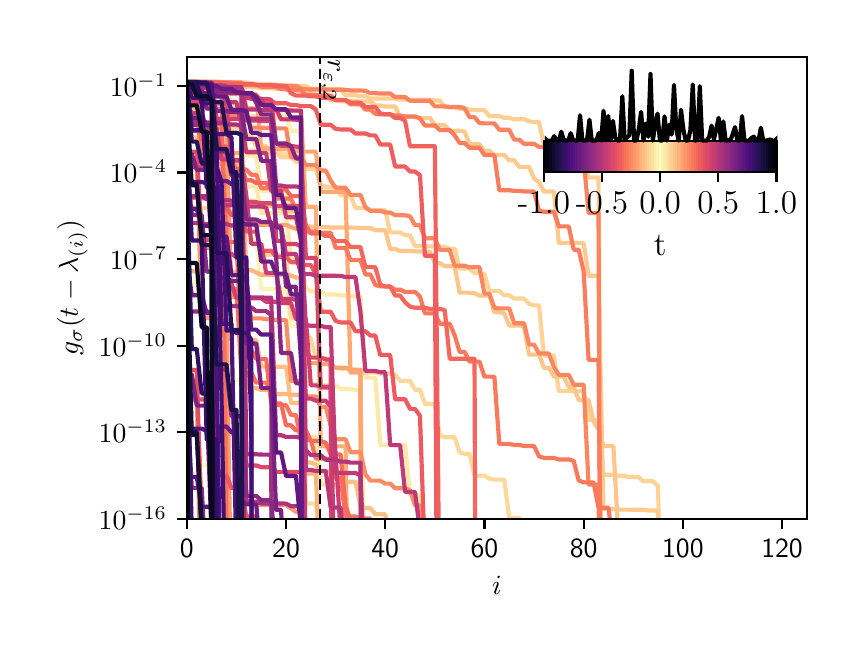
\begin{tikzpicture}
    \node at (0, 0) {%% Creator: Matplotlib, PGF backend
%%
%% To include the figure in your LaTeX document, write
%%   \input{<filename>.pgf}
%%
%% Make sure the required packages are loaded in your preamble
%%   \usepackage{pgf}
%%
%% Also ensure that all the required font packages are loaded; for instance,
%% the lmodern package is sometimes necessary when using math font.
%%   \usepackage{lmodern}
%%
%% Figures using additional raster images can only be included by \input if
%% they are in the same directory as the main LaTeX file. For loading figures
%% from other directories you can use the `import` package
%%   \usepackage{import}
%%
%% and then include the figures with
%%   \import{<path to file>}{<filename>.pgf}
%%
%% Matplotlib used the following preamble
%%   \def\mathdefault#1{#1}
%%   \everymath=\expandafter{\the\everymath\displaystyle}
%%   
%%   \usepackage{fontspec}
%%   \setmainfont{DejaVuSerif.ttf}[Path=\detokenize{C:/Users/fabio/Documents/Work/MasterThesis/Rand-SD/.venv/Lib/site-packages/matplotlib/mpl-data/fonts/ttf/}]
%%   \setsansfont{DejaVuSans.ttf}[Path=\detokenize{C:/Users/fabio/Documents/Work/MasterThesis/Rand-SD/.venv/Lib/site-packages/matplotlib/mpl-data/fonts/ttf/}]
%%   \setmonofont{DejaVuSansMono.ttf}[Path=\detokenize{C:/Users/fabio/Documents/Work/MasterThesis/Rand-SD/.venv/Lib/site-packages/matplotlib/mpl-data/fonts/ttf/}]
%%   \makeatletter\@ifpackageloaded{underscore}{}{\usepackage[strings]{underscore}}\makeatother
%%
\begingroup%
\makeatletter%
\begin{pgfpicture}%
\pgfpathrectangle{\pgfpointorigin}{\pgfqpoint{3.958241in}{2.931603in}}%
\pgfusepath{use as bounding box, clip}%
\begin{pgfscope}%
\pgfsetbuttcap%
\pgfsetmiterjoin%
\definecolor{currentfill}{rgb}{1.000000,1.000000,1.000000}%
\pgfsetfillcolor{currentfill}%
\pgfsetlinewidth{0.000000pt}%
\definecolor{currentstroke}{rgb}{1.000000,1.000000,1.000000}%
\pgfsetstrokecolor{currentstroke}%
\pgfsetdash{}{0pt}%
\pgfpathmoveto{\pgfqpoint{0.000000in}{0.000000in}}%
\pgfpathlineto{\pgfqpoint{3.958241in}{0.000000in}}%
\pgfpathlineto{\pgfqpoint{3.958241in}{2.931603in}}%
\pgfpathlineto{\pgfqpoint{0.000000in}{2.931603in}}%
\pgfpathlineto{\pgfqpoint{0.000000in}{0.000000in}}%
\pgfpathclose%
\pgfusepath{fill}%
\end{pgfscope}%
\begin{pgfscope}%
\pgfsetbuttcap%
\pgfsetmiterjoin%
\definecolor{currentfill}{rgb}{1.000000,1.000000,1.000000}%
\pgfsetfillcolor{currentfill}%
\pgfsetlinewidth{0.000000pt}%
\definecolor{currentstroke}{rgb}{0.000000,0.000000,0.000000}%
\pgfsetstrokecolor{currentstroke}%
\pgfsetstrokeopacity{0.000000}%
\pgfsetdash{}{0pt}%
\pgfpathmoveto{\pgfqpoint{0.749693in}{0.521603in}}%
\pgfpathlineto{\pgfqpoint{3.849693in}{0.521603in}}%
\pgfpathlineto{\pgfqpoint{3.849693in}{2.831603in}}%
\pgfpathlineto{\pgfqpoint{0.749693in}{2.831603in}}%
\pgfpathlineto{\pgfqpoint{0.749693in}{0.521603in}}%
\pgfpathclose%
\pgfusepath{fill}%
\end{pgfscope}%
\begin{pgfscope}%
\pgfsetbuttcap%
\pgfsetroundjoin%
\definecolor{currentfill}{rgb}{0.000000,0.000000,0.000000}%
\pgfsetfillcolor{currentfill}%
\pgfsetlinewidth{0.803000pt}%
\definecolor{currentstroke}{rgb}{0.000000,0.000000,0.000000}%
\pgfsetstrokecolor{currentstroke}%
\pgfsetdash{}{0pt}%
\pgfsys@defobject{currentmarker}{\pgfqpoint{0.000000in}{-0.048611in}}{\pgfqpoint{0.000000in}{0.000000in}}{%
\pgfpathmoveto{\pgfqpoint{0.000000in}{0.000000in}}%
\pgfpathlineto{\pgfqpoint{0.000000in}{-0.048611in}}%
\pgfusepath{stroke,fill}%
}%
\begin{pgfscope}%
\pgfsys@transformshift{0.749693in}{0.521603in}%
\pgfsys@useobject{currentmarker}{}%
\end{pgfscope}%
\end{pgfscope}%
\begin{pgfscope}%
\definecolor{textcolor}{rgb}{0.000000,0.000000,0.000000}%
\pgfsetstrokecolor{textcolor}%
\pgfsetfillcolor{textcolor}%
\pgftext[x=0.749693in,y=0.424381in,,top]{\color{textcolor}{\sffamily\fontsize{10.000000}{12.000000}\selectfont\catcode`\^=\active\def^{\ifmmode\sp\else\^{}\fi}\catcode`\%=\active\def%{\%}0}}%
\end{pgfscope}%
\begin{pgfscope}%
\pgfsetbuttcap%
\pgfsetroundjoin%
\definecolor{currentfill}{rgb}{0.000000,0.000000,0.000000}%
\pgfsetfillcolor{currentfill}%
\pgfsetlinewidth{0.803000pt}%
\definecolor{currentstroke}{rgb}{0.000000,0.000000,0.000000}%
\pgfsetstrokecolor{currentstroke}%
\pgfsetdash{}{0pt}%
\pgfsys@defobject{currentmarker}{\pgfqpoint{0.000000in}{-0.048611in}}{\pgfqpoint{0.000000in}{0.000000in}}{%
\pgfpathmoveto{\pgfqpoint{0.000000in}{0.000000in}}%
\pgfpathlineto{\pgfqpoint{0.000000in}{-0.048611in}}%
\pgfusepath{stroke,fill}%
}%
\begin{pgfscope}%
\pgfsys@transformshift{1.245693in}{0.521603in}%
\pgfsys@useobject{currentmarker}{}%
\end{pgfscope}%
\end{pgfscope}%
\begin{pgfscope}%
\definecolor{textcolor}{rgb}{0.000000,0.000000,0.000000}%
\pgfsetstrokecolor{textcolor}%
\pgfsetfillcolor{textcolor}%
\pgftext[x=1.245693in,y=0.424381in,,top]{\color{textcolor}{\sffamily\fontsize{10.000000}{12.000000}\selectfont\catcode`\^=\active\def^{\ifmmode\sp\else\^{}\fi}\catcode`\%=\active\def%{\%}20}}%
\end{pgfscope}%
\begin{pgfscope}%
\pgfsetbuttcap%
\pgfsetroundjoin%
\definecolor{currentfill}{rgb}{0.000000,0.000000,0.000000}%
\pgfsetfillcolor{currentfill}%
\pgfsetlinewidth{0.803000pt}%
\definecolor{currentstroke}{rgb}{0.000000,0.000000,0.000000}%
\pgfsetstrokecolor{currentstroke}%
\pgfsetdash{}{0pt}%
\pgfsys@defobject{currentmarker}{\pgfqpoint{0.000000in}{-0.048611in}}{\pgfqpoint{0.000000in}{0.000000in}}{%
\pgfpathmoveto{\pgfqpoint{0.000000in}{0.000000in}}%
\pgfpathlineto{\pgfqpoint{0.000000in}{-0.048611in}}%
\pgfusepath{stroke,fill}%
}%
\begin{pgfscope}%
\pgfsys@transformshift{1.741693in}{0.521603in}%
\pgfsys@useobject{currentmarker}{}%
\end{pgfscope}%
\end{pgfscope}%
\begin{pgfscope}%
\definecolor{textcolor}{rgb}{0.000000,0.000000,0.000000}%
\pgfsetstrokecolor{textcolor}%
\pgfsetfillcolor{textcolor}%
\pgftext[x=1.741693in,y=0.424381in,,top]{\color{textcolor}{\sffamily\fontsize{10.000000}{12.000000}\selectfont\catcode`\^=\active\def^{\ifmmode\sp\else\^{}\fi}\catcode`\%=\active\def%{\%}40}}%
\end{pgfscope}%
\begin{pgfscope}%
\pgfsetbuttcap%
\pgfsetroundjoin%
\definecolor{currentfill}{rgb}{0.000000,0.000000,0.000000}%
\pgfsetfillcolor{currentfill}%
\pgfsetlinewidth{0.803000pt}%
\definecolor{currentstroke}{rgb}{0.000000,0.000000,0.000000}%
\pgfsetstrokecolor{currentstroke}%
\pgfsetdash{}{0pt}%
\pgfsys@defobject{currentmarker}{\pgfqpoint{0.000000in}{-0.048611in}}{\pgfqpoint{0.000000in}{0.000000in}}{%
\pgfpathmoveto{\pgfqpoint{0.000000in}{0.000000in}}%
\pgfpathlineto{\pgfqpoint{0.000000in}{-0.048611in}}%
\pgfusepath{stroke,fill}%
}%
\begin{pgfscope}%
\pgfsys@transformshift{2.237693in}{0.521603in}%
\pgfsys@useobject{currentmarker}{}%
\end{pgfscope}%
\end{pgfscope}%
\begin{pgfscope}%
\definecolor{textcolor}{rgb}{0.000000,0.000000,0.000000}%
\pgfsetstrokecolor{textcolor}%
\pgfsetfillcolor{textcolor}%
\pgftext[x=2.237693in,y=0.424381in,,top]{\color{textcolor}{\sffamily\fontsize{10.000000}{12.000000}\selectfont\catcode`\^=\active\def^{\ifmmode\sp\else\^{}\fi}\catcode`\%=\active\def%{\%}60}}%
\end{pgfscope}%
\begin{pgfscope}%
\pgfsetbuttcap%
\pgfsetroundjoin%
\definecolor{currentfill}{rgb}{0.000000,0.000000,0.000000}%
\pgfsetfillcolor{currentfill}%
\pgfsetlinewidth{0.803000pt}%
\definecolor{currentstroke}{rgb}{0.000000,0.000000,0.000000}%
\pgfsetstrokecolor{currentstroke}%
\pgfsetdash{}{0pt}%
\pgfsys@defobject{currentmarker}{\pgfqpoint{0.000000in}{-0.048611in}}{\pgfqpoint{0.000000in}{0.000000in}}{%
\pgfpathmoveto{\pgfqpoint{0.000000in}{0.000000in}}%
\pgfpathlineto{\pgfqpoint{0.000000in}{-0.048611in}}%
\pgfusepath{stroke,fill}%
}%
\begin{pgfscope}%
\pgfsys@transformshift{2.733693in}{0.521603in}%
\pgfsys@useobject{currentmarker}{}%
\end{pgfscope}%
\end{pgfscope}%
\begin{pgfscope}%
\definecolor{textcolor}{rgb}{0.000000,0.000000,0.000000}%
\pgfsetstrokecolor{textcolor}%
\pgfsetfillcolor{textcolor}%
\pgftext[x=2.733693in,y=0.424381in,,top]{\color{textcolor}{\sffamily\fontsize{10.000000}{12.000000}\selectfont\catcode`\^=\active\def^{\ifmmode\sp\else\^{}\fi}\catcode`\%=\active\def%{\%}80}}%
\end{pgfscope}%
\begin{pgfscope}%
\pgfsetbuttcap%
\pgfsetroundjoin%
\definecolor{currentfill}{rgb}{0.000000,0.000000,0.000000}%
\pgfsetfillcolor{currentfill}%
\pgfsetlinewidth{0.803000pt}%
\definecolor{currentstroke}{rgb}{0.000000,0.000000,0.000000}%
\pgfsetstrokecolor{currentstroke}%
\pgfsetdash{}{0pt}%
\pgfsys@defobject{currentmarker}{\pgfqpoint{0.000000in}{-0.048611in}}{\pgfqpoint{0.000000in}{0.000000in}}{%
\pgfpathmoveto{\pgfqpoint{0.000000in}{0.000000in}}%
\pgfpathlineto{\pgfqpoint{0.000000in}{-0.048611in}}%
\pgfusepath{stroke,fill}%
}%
\begin{pgfscope}%
\pgfsys@transformshift{3.229693in}{0.521603in}%
\pgfsys@useobject{currentmarker}{}%
\end{pgfscope}%
\end{pgfscope}%
\begin{pgfscope}%
\definecolor{textcolor}{rgb}{0.000000,0.000000,0.000000}%
\pgfsetstrokecolor{textcolor}%
\pgfsetfillcolor{textcolor}%
\pgftext[x=3.229693in,y=0.424381in,,top]{\color{textcolor}{\sffamily\fontsize{10.000000}{12.000000}\selectfont\catcode`\^=\active\def^{\ifmmode\sp\else\^{}\fi}\catcode`\%=\active\def%{\%}100}}%
\end{pgfscope}%
\begin{pgfscope}%
\pgfsetbuttcap%
\pgfsetroundjoin%
\definecolor{currentfill}{rgb}{0.000000,0.000000,0.000000}%
\pgfsetfillcolor{currentfill}%
\pgfsetlinewidth{0.803000pt}%
\definecolor{currentstroke}{rgb}{0.000000,0.000000,0.000000}%
\pgfsetstrokecolor{currentstroke}%
\pgfsetdash{}{0pt}%
\pgfsys@defobject{currentmarker}{\pgfqpoint{0.000000in}{-0.048611in}}{\pgfqpoint{0.000000in}{0.000000in}}{%
\pgfpathmoveto{\pgfqpoint{0.000000in}{0.000000in}}%
\pgfpathlineto{\pgfqpoint{0.000000in}{-0.048611in}}%
\pgfusepath{stroke,fill}%
}%
\begin{pgfscope}%
\pgfsys@transformshift{3.725693in}{0.521603in}%
\pgfsys@useobject{currentmarker}{}%
\end{pgfscope}%
\end{pgfscope}%
\begin{pgfscope}%
\definecolor{textcolor}{rgb}{0.000000,0.000000,0.000000}%
\pgfsetstrokecolor{textcolor}%
\pgfsetfillcolor{textcolor}%
\pgftext[x=3.725693in,y=0.424381in,,top]{\color{textcolor}{\sffamily\fontsize{10.000000}{12.000000}\selectfont\catcode`\^=\active\def^{\ifmmode\sp\else\^{}\fi}\catcode`\%=\active\def%{\%}120}}%
\end{pgfscope}%
\begin{pgfscope}%
\definecolor{textcolor}{rgb}{0.000000,0.000000,0.000000}%
\pgfsetstrokecolor{textcolor}%
\pgfsetfillcolor{textcolor}%
\pgftext[x=2.299693in,y=0.234413in,,top]{\color{textcolor}{\sffamily\fontsize{10.000000}{12.000000}\selectfont\catcode`\^=\active\def^{\ifmmode\sp\else\^{}\fi}\catcode`\%=\active\def%{\%}$i$}}%
\end{pgfscope}%
\begin{pgfscope}%
\pgfsetbuttcap%
\pgfsetroundjoin%
\definecolor{currentfill}{rgb}{0.000000,0.000000,0.000000}%
\pgfsetfillcolor{currentfill}%
\pgfsetlinewidth{0.803000pt}%
\definecolor{currentstroke}{rgb}{0.000000,0.000000,0.000000}%
\pgfsetstrokecolor{currentstroke}%
\pgfsetdash{}{0pt}%
\pgfsys@defobject{currentmarker}{\pgfqpoint{-0.048611in}{0.000000in}}{\pgfqpoint{-0.000000in}{0.000000in}}{%
\pgfpathmoveto{\pgfqpoint{-0.000000in}{0.000000in}}%
\pgfpathlineto{\pgfqpoint{-0.048611in}{0.000000in}}%
\pgfusepath{stroke,fill}%
}%
\begin{pgfscope}%
\pgfsys@transformshift{0.749693in}{0.521603in}%
\pgfsys@useobject{currentmarker}{}%
\end{pgfscope}%
\end{pgfscope}%
\begin{pgfscope}%
\definecolor{textcolor}{rgb}{0.000000,0.000000,0.000000}%
\pgfsetstrokecolor{textcolor}%
\pgfsetfillcolor{textcolor}%
\pgftext[x=0.309105in, y=0.468842in, left, base]{\color{textcolor}{\sffamily\fontsize{10.000000}{12.000000}\selectfont\catcode`\^=\active\def^{\ifmmode\sp\else\^{}\fi}\catcode`\%=\active\def%{\%}$\mathdefault{10^{-16}}$}}%
\end{pgfscope}%
\begin{pgfscope}%
\pgfsetbuttcap%
\pgfsetroundjoin%
\definecolor{currentfill}{rgb}{0.000000,0.000000,0.000000}%
\pgfsetfillcolor{currentfill}%
\pgfsetlinewidth{0.803000pt}%
\definecolor{currentstroke}{rgb}{0.000000,0.000000,0.000000}%
\pgfsetstrokecolor{currentstroke}%
\pgfsetdash{}{0pt}%
\pgfsys@defobject{currentmarker}{\pgfqpoint{-0.048611in}{0.000000in}}{\pgfqpoint{-0.000000in}{0.000000in}}{%
\pgfpathmoveto{\pgfqpoint{-0.000000in}{0.000000in}}%
\pgfpathlineto{\pgfqpoint{-0.048611in}{0.000000in}}%
\pgfusepath{stroke,fill}%
}%
\begin{pgfscope}%
\pgfsys@transformshift{0.749693in}{0.954728in}%
\pgfsys@useobject{currentmarker}{}%
\end{pgfscope}%
\end{pgfscope}%
\begin{pgfscope}%
\definecolor{textcolor}{rgb}{0.000000,0.000000,0.000000}%
\pgfsetstrokecolor{textcolor}%
\pgfsetfillcolor{textcolor}%
\pgftext[x=0.309105in, y=0.901967in, left, base]{\color{textcolor}{\sffamily\fontsize{10.000000}{12.000000}\selectfont\catcode`\^=\active\def^{\ifmmode\sp\else\^{}\fi}\catcode`\%=\active\def%{\%}$\mathdefault{10^{-13}}$}}%
\end{pgfscope}%
\begin{pgfscope}%
\pgfsetbuttcap%
\pgfsetroundjoin%
\definecolor{currentfill}{rgb}{0.000000,0.000000,0.000000}%
\pgfsetfillcolor{currentfill}%
\pgfsetlinewidth{0.803000pt}%
\definecolor{currentstroke}{rgb}{0.000000,0.000000,0.000000}%
\pgfsetstrokecolor{currentstroke}%
\pgfsetdash{}{0pt}%
\pgfsys@defobject{currentmarker}{\pgfqpoint{-0.048611in}{0.000000in}}{\pgfqpoint{-0.000000in}{0.000000in}}{%
\pgfpathmoveto{\pgfqpoint{-0.000000in}{0.000000in}}%
\pgfpathlineto{\pgfqpoint{-0.048611in}{0.000000in}}%
\pgfusepath{stroke,fill}%
}%
\begin{pgfscope}%
\pgfsys@transformshift{0.749693in}{1.387853in}%
\pgfsys@useobject{currentmarker}{}%
\end{pgfscope}%
\end{pgfscope}%
\begin{pgfscope}%
\definecolor{textcolor}{rgb}{0.000000,0.000000,0.000000}%
\pgfsetstrokecolor{textcolor}%
\pgfsetfillcolor{textcolor}%
\pgftext[x=0.309105in, y=1.335092in, left, base]{\color{textcolor}{\sffamily\fontsize{10.000000}{12.000000}\selectfont\catcode`\^=\active\def^{\ifmmode\sp\else\^{}\fi}\catcode`\%=\active\def%{\%}$\mathdefault{10^{-10}}$}}%
\end{pgfscope}%
\begin{pgfscope}%
\pgfsetbuttcap%
\pgfsetroundjoin%
\definecolor{currentfill}{rgb}{0.000000,0.000000,0.000000}%
\pgfsetfillcolor{currentfill}%
\pgfsetlinewidth{0.803000pt}%
\definecolor{currentstroke}{rgb}{0.000000,0.000000,0.000000}%
\pgfsetstrokecolor{currentstroke}%
\pgfsetdash{}{0pt}%
\pgfsys@defobject{currentmarker}{\pgfqpoint{-0.048611in}{0.000000in}}{\pgfqpoint{-0.000000in}{0.000000in}}{%
\pgfpathmoveto{\pgfqpoint{-0.000000in}{0.000000in}}%
\pgfpathlineto{\pgfqpoint{-0.048611in}{0.000000in}}%
\pgfusepath{stroke,fill}%
}%
\begin{pgfscope}%
\pgfsys@transformshift{0.749693in}{1.820978in}%
\pgfsys@useobject{currentmarker}{}%
\end{pgfscope}%
\end{pgfscope}%
\begin{pgfscope}%
\definecolor{textcolor}{rgb}{0.000000,0.000000,0.000000}%
\pgfsetstrokecolor{textcolor}%
\pgfsetfillcolor{textcolor}%
\pgftext[x=0.364468in, y=1.768217in, left, base]{\color{textcolor}{\sffamily\fontsize{10.000000}{12.000000}\selectfont\catcode`\^=\active\def^{\ifmmode\sp\else\^{}\fi}\catcode`\%=\active\def%{\%}$\mathdefault{10^{-7}}$}}%
\end{pgfscope}%
\begin{pgfscope}%
\pgfsetbuttcap%
\pgfsetroundjoin%
\definecolor{currentfill}{rgb}{0.000000,0.000000,0.000000}%
\pgfsetfillcolor{currentfill}%
\pgfsetlinewidth{0.803000pt}%
\definecolor{currentstroke}{rgb}{0.000000,0.000000,0.000000}%
\pgfsetstrokecolor{currentstroke}%
\pgfsetdash{}{0pt}%
\pgfsys@defobject{currentmarker}{\pgfqpoint{-0.048611in}{0.000000in}}{\pgfqpoint{-0.000000in}{0.000000in}}{%
\pgfpathmoveto{\pgfqpoint{-0.000000in}{0.000000in}}%
\pgfpathlineto{\pgfqpoint{-0.048611in}{0.000000in}}%
\pgfusepath{stroke,fill}%
}%
\begin{pgfscope}%
\pgfsys@transformshift{0.749693in}{2.254103in}%
\pgfsys@useobject{currentmarker}{}%
\end{pgfscope}%
\end{pgfscope}%
\begin{pgfscope}%
\definecolor{textcolor}{rgb}{0.000000,0.000000,0.000000}%
\pgfsetstrokecolor{textcolor}%
\pgfsetfillcolor{textcolor}%
\pgftext[x=0.364468in, y=2.201342in, left, base]{\color{textcolor}{\sffamily\fontsize{10.000000}{12.000000}\selectfont\catcode`\^=\active\def^{\ifmmode\sp\else\^{}\fi}\catcode`\%=\active\def%{\%}$\mathdefault{10^{-4}}$}}%
\end{pgfscope}%
\begin{pgfscope}%
\pgfsetbuttcap%
\pgfsetroundjoin%
\definecolor{currentfill}{rgb}{0.000000,0.000000,0.000000}%
\pgfsetfillcolor{currentfill}%
\pgfsetlinewidth{0.803000pt}%
\definecolor{currentstroke}{rgb}{0.000000,0.000000,0.000000}%
\pgfsetstrokecolor{currentstroke}%
\pgfsetdash{}{0pt}%
\pgfsys@defobject{currentmarker}{\pgfqpoint{-0.048611in}{0.000000in}}{\pgfqpoint{-0.000000in}{0.000000in}}{%
\pgfpathmoveto{\pgfqpoint{-0.000000in}{0.000000in}}%
\pgfpathlineto{\pgfqpoint{-0.048611in}{0.000000in}}%
\pgfusepath{stroke,fill}%
}%
\begin{pgfscope}%
\pgfsys@transformshift{0.749693in}{2.687228in}%
\pgfsys@useobject{currentmarker}{}%
\end{pgfscope}%
\end{pgfscope}%
\begin{pgfscope}%
\definecolor{textcolor}{rgb}{0.000000,0.000000,0.000000}%
\pgfsetstrokecolor{textcolor}%
\pgfsetfillcolor{textcolor}%
\pgftext[x=0.364468in, y=2.634467in, left, base]{\color{textcolor}{\sffamily\fontsize{10.000000}{12.000000}\selectfont\catcode`\^=\active\def^{\ifmmode\sp\else\^{}\fi}\catcode`\%=\active\def%{\%}$\mathdefault{10^{-1}}$}}%
\end{pgfscope}%
\begin{pgfscope}%
\definecolor{textcolor}{rgb}{0.000000,0.000000,0.000000}%
\pgfsetstrokecolor{textcolor}%
\pgfsetfillcolor{textcolor}%
\pgftext[x=0.253550in,y=1.676603in,,bottom,rotate=90.000000]{\color{textcolor}{\sffamily\fontsize{10.000000}{12.000000}\selectfont\catcode`\^=\active\def^{\ifmmode\sp\else\^{}\fi}\catcode`\%=\active\def%{\%}$g_{\sigma}(t - \lambda_{(i)})$}}%
\end{pgfscope}%
\begin{pgfscope}%
\pgfpathrectangle{\pgfqpoint{0.749693in}{0.521603in}}{\pgfqpoint{3.100000in}{2.310000in}}%
\pgfusepath{clip}%
\pgfsetrectcap%
\pgfsetroundjoin%
\pgfsetlinewidth{1.505625pt}%
\definecolor{currentstroke}{rgb}{0.987053,0.991438,0.749504}%
\pgfsetstrokecolor{currentstroke}%
\pgfsetdash{}{0pt}%
\pgfpathmoveto{\pgfqpoint{0.749693in}{0.980593in}}%
\pgfpathlineto{\pgfqpoint{0.799293in}{0.980290in}}%
\pgfpathlineto{\pgfqpoint{0.824093in}{0.788421in}}%
\pgfpathlineto{\pgfqpoint{0.948093in}{0.788386in}}%
\pgfpathlineto{\pgfqpoint{0.968223in}{0.511603in}}%
\pgfpathlineto{\pgfqpoint{0.968223in}{0.511603in}}%
\pgfusepath{stroke}%
\end{pgfscope}%
\begin{pgfscope}%
\pgfpathrectangle{\pgfqpoint{0.749693in}{0.521603in}}{\pgfqpoint{3.100000in}{2.310000in}}%
\pgfusepath{clip}%
\pgfsetrectcap%
\pgfsetroundjoin%
\pgfsetlinewidth{1.505625pt}%
\definecolor{currentstroke}{rgb}{0.987691,0.977154,0.734536}%
\pgfsetstrokecolor{currentstroke}%
\pgfsetdash{}{0pt}%
\pgfpathmoveto{\pgfqpoint{0.749693in}{1.709115in}}%
\pgfpathlineto{\pgfqpoint{0.799293in}{1.708387in}}%
\pgfpathlineto{\pgfqpoint{0.824093in}{1.520385in}}%
\pgfpathlineto{\pgfqpoint{0.948093in}{1.520345in}}%
\pgfpathlineto{\pgfqpoint{0.972893in}{1.217082in}}%
\pgfpathlineto{\pgfqpoint{1.022493in}{1.216187in}}%
\pgfpathlineto{\pgfqpoint{1.045763in}{0.511603in}}%
\pgfpathlineto{\pgfqpoint{1.045763in}{0.511603in}}%
\pgfusepath{stroke}%
\end{pgfscope}%
\begin{pgfscope}%
\pgfpathrectangle{\pgfqpoint{0.749693in}{0.521603in}}{\pgfqpoint{3.100000in}{2.310000in}}%
\pgfusepath{clip}%
\pgfsetrectcap%
\pgfsetroundjoin%
\pgfsetlinewidth{1.505625pt}%
\definecolor{currentstroke}{rgb}{0.988717,0.955742,0.712242}%
\pgfsetstrokecolor{currentstroke}%
\pgfsetdash{}{0pt}%
\pgfpathmoveto{\pgfqpoint{0.749693in}{2.554702in}}%
\pgfpathlineto{\pgfqpoint{0.799293in}{2.554418in}}%
\pgfpathlineto{\pgfqpoint{0.824093in}{2.476100in}}%
\pgfpathlineto{\pgfqpoint{0.948093in}{2.476083in}}%
\pgfpathlineto{\pgfqpoint{0.972893in}{2.332790in}}%
\pgfpathlineto{\pgfqpoint{1.022493in}{2.332341in}}%
\pgfpathlineto{\pgfqpoint{1.047293in}{1.918026in}}%
\pgfpathlineto{\pgfqpoint{1.096893in}{1.918026in}}%
\pgfpathlineto{\pgfqpoint{1.121693in}{1.671646in}}%
\pgfpathlineto{\pgfqpoint{1.245693in}{1.670905in}}%
\pgfpathlineto{\pgfqpoint{1.270493in}{1.487623in}}%
\pgfpathlineto{\pgfqpoint{1.320093in}{1.487623in}}%
\pgfpathlineto{\pgfqpoint{1.325178in}{0.511603in}}%
\pgfpathlineto{\pgfqpoint{1.325178in}{0.511603in}}%
\pgfusepath{stroke}%
\end{pgfscope}%
\begin{pgfscope}%
\pgfpathrectangle{\pgfqpoint{0.749693in}{0.521603in}}{\pgfqpoint{3.100000in}{2.310000in}}%
\pgfusepath{clip}%
\pgfsetrectcap%
\pgfsetroundjoin%
\pgfsetlinewidth{1.505625pt}%
\definecolor{currentstroke}{rgb}{0.989434,0.941470,0.697519}%
\pgfsetstrokecolor{currentstroke}%
\pgfsetdash{}{0pt}%
\pgfpathmoveto{\pgfqpoint{0.749693in}{2.706444in}}%
\pgfpathlineto{\pgfqpoint{0.799293in}{2.706442in}}%
\pgfpathlineto{\pgfqpoint{0.824093in}{2.689767in}}%
\pgfpathlineto{\pgfqpoint{0.948093in}{2.689762in}}%
\pgfpathlineto{\pgfqpoint{0.972893in}{2.658396in}}%
\pgfpathlineto{\pgfqpoint{1.022493in}{2.658236in}}%
\pgfpathlineto{\pgfqpoint{1.047293in}{2.628712in}}%
\pgfpathlineto{\pgfqpoint{1.096893in}{2.628712in}}%
\pgfpathlineto{\pgfqpoint{1.121693in}{2.539876in}}%
\pgfpathlineto{\pgfqpoint{1.245693in}{2.539578in}}%
\pgfpathlineto{\pgfqpoint{1.270493in}{2.461537in}}%
\pgfpathlineto{\pgfqpoint{1.320093in}{2.461537in}}%
\pgfpathlineto{\pgfqpoint{1.335563in}{0.511603in}}%
\pgfpathlineto{\pgfqpoint{1.335563in}{0.511603in}}%
\pgfusepath{stroke}%
\end{pgfscope}%
\begin{pgfscope}%
\pgfpathrectangle{\pgfqpoint{0.749693in}{0.521603in}}{\pgfqpoint{3.100000in}{2.310000in}}%
\pgfusepath{clip}%
\pgfsetrectcap%
\pgfsetroundjoin%
\pgfsetlinewidth{1.505625pt}%
\definecolor{currentstroke}{rgb}{0.990570,0.920049,0.675675}%
\pgfsetstrokecolor{currentstroke}%
\pgfsetdash{}{0pt}%
\pgfpathmoveto{\pgfqpoint{0.749693in}{2.693399in}}%
\pgfpathlineto{\pgfqpoint{0.799293in}{2.693399in}}%
\pgfpathlineto{\pgfqpoint{0.824093in}{2.666199in}}%
\pgfpathlineto{\pgfqpoint{0.948093in}{2.666052in}}%
\pgfpathlineto{\pgfqpoint{0.972893in}{2.597345in}}%
\pgfpathlineto{\pgfqpoint{1.022493in}{2.597345in}}%
\pgfpathlineto{\pgfqpoint{1.047293in}{2.338490in}}%
\pgfpathlineto{\pgfqpoint{1.096893in}{2.338045in}}%
\pgfpathlineto{\pgfqpoint{1.121693in}{2.161398in}}%
\pgfpathlineto{\pgfqpoint{1.245693in}{2.161371in}}%
\pgfpathlineto{\pgfqpoint{1.270493in}{2.020320in}}%
\pgfpathlineto{\pgfqpoint{1.320093in}{2.019716in}}%
\pgfpathlineto{\pgfqpoint{1.344893in}{1.201349in}}%
\pgfpathlineto{\pgfqpoint{1.369693in}{1.196889in}}%
\pgfpathlineto{\pgfqpoint{1.419293in}{1.196889in}}%
\pgfpathlineto{\pgfqpoint{1.444093in}{1.191212in}}%
\pgfpathlineto{\pgfqpoint{1.493693in}{1.191212in}}%
\pgfpathlineto{\pgfqpoint{1.518493in}{1.171097in}}%
\pgfpathlineto{\pgfqpoint{1.568093in}{1.171097in}}%
\pgfpathlineto{\pgfqpoint{1.592893in}{1.164460in}}%
\pgfpathlineto{\pgfqpoint{1.617693in}{1.164460in}}%
\pgfpathlineto{\pgfqpoint{1.632460in}{0.511603in}}%
\pgfpathlineto{\pgfqpoint{1.632460in}{0.511603in}}%
\pgfusepath{stroke}%
\end{pgfscope}%
\begin{pgfscope}%
\pgfpathrectangle{\pgfqpoint{0.749693in}{0.521603in}}{\pgfqpoint{3.100000in}{2.310000in}}%
\pgfusepath{clip}%
\pgfsetrectcap%
\pgfsetroundjoin%
\pgfsetlinewidth{1.505625pt}%
\definecolor{currentstroke}{rgb}{0.991332,0.905763,0.661309}%
\pgfsetstrokecolor{currentstroke}%
\pgfsetdash{}{0pt}%
\pgfpathmoveto{\pgfqpoint{0.749693in}{2.324888in}}%
\pgfpathlineto{\pgfqpoint{0.774493in}{2.322641in}}%
\pgfpathlineto{\pgfqpoint{0.824093in}{2.322641in}}%
\pgfpathlineto{\pgfqpoint{0.848893in}{2.319776in}}%
\pgfpathlineto{\pgfqpoint{0.898493in}{2.319776in}}%
\pgfpathlineto{\pgfqpoint{0.923293in}{2.309582in}}%
\pgfpathlineto{\pgfqpoint{0.972893in}{2.309582in}}%
\pgfpathlineto{\pgfqpoint{0.997693in}{2.306204in}}%
\pgfpathlineto{\pgfqpoint{1.022493in}{2.306204in}}%
\pgfpathlineto{\pgfqpoint{1.047293in}{2.183207in}}%
\pgfpathlineto{\pgfqpoint{1.096893in}{2.183207in}}%
\pgfpathlineto{\pgfqpoint{1.121693in}{2.050766in}}%
\pgfpathlineto{\pgfqpoint{1.245693in}{2.050176in}}%
\pgfpathlineto{\pgfqpoint{1.270493in}{1.823925in}}%
\pgfpathlineto{\pgfqpoint{1.320093in}{1.823925in}}%
\pgfpathlineto{\pgfqpoint{1.344893in}{1.675860in}}%
\pgfpathlineto{\pgfqpoint{1.369693in}{1.659130in}}%
\pgfpathlineto{\pgfqpoint{1.419293in}{1.659130in}}%
\pgfpathlineto{\pgfqpoint{1.444093in}{1.643181in}}%
\pgfpathlineto{\pgfqpoint{1.493693in}{1.643181in}}%
\pgfpathlineto{\pgfqpoint{1.518493in}{1.638771in}}%
\pgfpathlineto{\pgfqpoint{1.543293in}{1.638771in}}%
\pgfpathlineto{\pgfqpoint{1.568093in}{1.635204in}}%
\pgfpathlineto{\pgfqpoint{1.617693in}{1.635204in}}%
\pgfpathlineto{\pgfqpoint{1.642493in}{1.228484in}}%
\pgfpathlineto{\pgfqpoint{1.692093in}{1.227592in}}%
\pgfpathlineto{\pgfqpoint{1.716893in}{0.890977in}}%
\pgfpathlineto{\pgfqpoint{1.840893in}{0.890927in}}%
\pgfpathlineto{\pgfqpoint{1.865693in}{0.640192in}}%
\pgfpathlineto{\pgfqpoint{1.915293in}{0.639144in}}%
\pgfpathlineto{\pgfqpoint{1.915917in}{0.511603in}}%
\pgfpathlineto{\pgfqpoint{1.915917in}{0.511603in}}%
\pgfusepath{stroke}%
\end{pgfscope}%
\begin{pgfscope}%
\pgfpathrectangle{\pgfqpoint{0.749693in}{0.521603in}}{\pgfqpoint{3.100000in}{2.310000in}}%
\pgfusepath{clip}%
\pgfsetrectcap%
\pgfsetroundjoin%
\pgfsetlinewidth{1.505625pt}%
\definecolor{currentstroke}{rgb}{0.992440,0.884330,0.640099}%
\pgfsetstrokecolor{currentstroke}%
\pgfsetdash{}{0pt}%
\pgfpathmoveto{\pgfqpoint{0.749693in}{2.706374in}}%
\pgfpathlineto{\pgfqpoint{1.022493in}{2.705895in}}%
\pgfpathlineto{\pgfqpoint{1.047293in}{2.541564in}}%
\pgfpathlineto{\pgfqpoint{1.072093in}{2.534832in}}%
\pgfpathlineto{\pgfqpoint{1.121693in}{2.534832in}}%
\pgfpathlineto{\pgfqpoint{1.146493in}{2.528340in}}%
\pgfpathlineto{\pgfqpoint{1.196093in}{2.528340in}}%
\pgfpathlineto{\pgfqpoint{1.220893in}{2.526532in}}%
\pgfpathlineto{\pgfqpoint{1.245693in}{2.526532in}}%
\pgfpathlineto{\pgfqpoint{1.270493in}{2.525066in}}%
\pgfpathlineto{\pgfqpoint{1.320093in}{2.525066in}}%
\pgfpathlineto{\pgfqpoint{1.344893in}{0.930962in}}%
\pgfpathlineto{\pgfqpoint{1.394493in}{0.930962in}}%
\pgfpathlineto{\pgfqpoint{1.419293in}{0.693281in}}%
\pgfpathlineto{\pgfqpoint{1.543293in}{0.692246in}}%
\pgfpathlineto{\pgfqpoint{1.554965in}{0.511603in}}%
\pgfpathlineto{\pgfqpoint{1.554965in}{0.511603in}}%
\pgfusepath{stroke}%
\end{pgfscope}%
\begin{pgfscope}%
\pgfpathrectangle{\pgfqpoint{0.749693in}{0.521603in}}{\pgfqpoint{3.100000in}{2.310000in}}%
\pgfusepath{clip}%
\pgfsetrectcap%
\pgfsetroundjoin%
\pgfsetlinewidth{1.505625pt}%
\definecolor{currentstroke}{rgb}{0.993170,0.870024,0.626189}%
\pgfsetstrokecolor{currentstroke}%
\pgfsetdash{}{0pt}%
\pgfpathmoveto{\pgfqpoint{0.749693in}{2.672875in}}%
\pgfpathlineto{\pgfqpoint{0.848893in}{2.672240in}}%
\pgfpathlineto{\pgfqpoint{0.898493in}{2.671445in}}%
\pgfpathlineto{\pgfqpoint{0.923293in}{2.671445in}}%
\pgfpathlineto{\pgfqpoint{0.948093in}{2.668480in}}%
\pgfpathlineto{\pgfqpoint{0.997693in}{2.668480in}}%
\pgfpathlineto{\pgfqpoint{1.022493in}{2.665215in}}%
\pgfpathlineto{\pgfqpoint{1.047293in}{2.363532in}}%
\pgfpathlineto{\pgfqpoint{1.072093in}{2.363532in}}%
\pgfpathlineto{\pgfqpoint{1.096893in}{2.360392in}}%
\pgfpathlineto{\pgfqpoint{1.146493in}{2.360392in}}%
\pgfpathlineto{\pgfqpoint{1.171293in}{2.350744in}}%
\pgfpathlineto{\pgfqpoint{1.220893in}{2.350744in}}%
\pgfpathlineto{\pgfqpoint{1.245693in}{2.347986in}}%
\pgfpathlineto{\pgfqpoint{1.295293in}{2.347986in}}%
\pgfpathlineto{\pgfqpoint{1.320093in}{2.345807in}}%
\pgfpathlineto{\pgfqpoint{1.344893in}{0.598521in}}%
\pgfpathlineto{\pgfqpoint{1.394493in}{0.598521in}}%
\pgfpathlineto{\pgfqpoint{1.402792in}{0.511603in}}%
\pgfpathlineto{\pgfqpoint{1.402792in}{0.511603in}}%
\pgfusepath{stroke}%
\end{pgfscope}%
\begin{pgfscope}%
\pgfpathrectangle{\pgfqpoint{0.749693in}{0.521603in}}{\pgfqpoint{3.100000in}{2.310000in}}%
\pgfusepath{clip}%
\pgfsetrectcap%
\pgfsetroundjoin%
\pgfsetlinewidth{1.505625pt}%
\definecolor{currentstroke}{rgb}{0.994222,0.848540,0.605696}%
\pgfsetstrokecolor{currentstroke}%
\pgfsetdash{}{0pt}%
\pgfpathmoveto{\pgfqpoint{0.749693in}{2.078631in}}%
\pgfpathlineto{\pgfqpoint{0.799293in}{2.078631in}}%
\pgfpathlineto{\pgfqpoint{0.824093in}{2.075895in}}%
\pgfpathlineto{\pgfqpoint{0.848893in}{2.075895in}}%
\pgfpathlineto{\pgfqpoint{0.873693in}{2.072498in}}%
\pgfpathlineto{\pgfqpoint{0.923293in}{2.072498in}}%
\pgfpathlineto{\pgfqpoint{0.948093in}{2.060076in}}%
\pgfpathlineto{\pgfqpoint{0.997693in}{2.060076in}}%
\pgfpathlineto{\pgfqpoint{1.022493in}{2.046813in}}%
\pgfpathlineto{\pgfqpoint{1.047293in}{1.996220in}}%
\pgfpathlineto{\pgfqpoint{1.096893in}{1.996220in}}%
\pgfpathlineto{\pgfqpoint{1.121693in}{1.842290in}}%
\pgfpathlineto{\pgfqpoint{1.171293in}{1.842290in}}%
\pgfpathlineto{\pgfqpoint{1.196093in}{1.841153in}}%
\pgfpathlineto{\pgfqpoint{1.245693in}{1.841153in}}%
\pgfpathlineto{\pgfqpoint{1.270493in}{1.524894in}}%
\pgfpathlineto{\pgfqpoint{1.320093in}{1.524894in}}%
\pgfpathlineto{\pgfqpoint{1.344893in}{1.455081in}}%
\pgfpathlineto{\pgfqpoint{1.369693in}{1.422826in}}%
\pgfpathlineto{\pgfqpoint{1.394493in}{1.324634in}}%
\pgfpathlineto{\pgfqpoint{1.444093in}{1.324634in}}%
\pgfpathlineto{\pgfqpoint{1.468893in}{1.279117in}}%
\pgfpathlineto{\pgfqpoint{1.493693in}{1.279117in}}%
\pgfpathlineto{\pgfqpoint{1.518493in}{1.272717in}}%
\pgfpathlineto{\pgfqpoint{1.568093in}{1.272717in}}%
\pgfpathlineto{\pgfqpoint{1.592893in}{1.263404in}}%
\pgfpathlineto{\pgfqpoint{1.617693in}{1.263404in}}%
\pgfpathlineto{\pgfqpoint{1.642493in}{1.253149in}}%
\pgfpathlineto{\pgfqpoint{1.692093in}{1.253149in}}%
\pgfpathlineto{\pgfqpoint{1.716893in}{1.247579in}}%
\pgfpathlineto{\pgfqpoint{1.766493in}{1.247579in}}%
\pgfpathlineto{\pgfqpoint{1.791293in}{1.243187in}}%
\pgfpathlineto{\pgfqpoint{1.816093in}{1.211530in}}%
\pgfpathlineto{\pgfqpoint{1.865693in}{1.211530in}}%
\pgfpathlineto{\pgfqpoint{1.890493in}{1.167261in}}%
\pgfpathlineto{\pgfqpoint{1.915293in}{1.167261in}}%
\pgfpathlineto{\pgfqpoint{1.940093in}{1.096592in}}%
\pgfpathlineto{\pgfqpoint{1.989693in}{1.096592in}}%
\pgfpathlineto{\pgfqpoint{2.014493in}{0.938712in}}%
\pgfpathlineto{\pgfqpoint{2.039293in}{0.929730in}}%
\pgfpathlineto{\pgfqpoint{2.088893in}{0.929730in}}%
\pgfpathlineto{\pgfqpoint{2.113693in}{0.853871in}}%
\pgfpathlineto{\pgfqpoint{2.138493in}{0.847608in}}%
\pgfpathlineto{\pgfqpoint{2.163293in}{0.847608in}}%
\pgfpathlineto{\pgfqpoint{2.188093in}{0.737866in}}%
\pgfpathlineto{\pgfqpoint{2.237693in}{0.737866in}}%
\pgfpathlineto{\pgfqpoint{2.262493in}{0.723060in}}%
\pgfpathlineto{\pgfqpoint{2.287293in}{0.718168in}}%
\pgfpathlineto{\pgfqpoint{2.336893in}{0.718168in}}%
\pgfpathlineto{\pgfqpoint{2.361693in}{0.526213in}}%
\pgfpathlineto{\pgfqpoint{2.411293in}{0.526213in}}%
\pgfpathlineto{\pgfqpoint{2.426649in}{0.511603in}}%
\pgfpathlineto{\pgfqpoint{2.426649in}{0.511603in}}%
\pgfusepath{stroke}%
\end{pgfscope}%
\begin{pgfscope}%
\pgfpathrectangle{\pgfqpoint{0.749693in}{0.521603in}}{\pgfqpoint{3.100000in}{2.310000in}}%
\pgfusepath{clip}%
\pgfsetrectcap%
\pgfsetroundjoin%
\pgfsetlinewidth{1.505625pt}%
\definecolor{currentstroke}{rgb}{0.995131,0.827052,0.585701}%
\pgfsetstrokecolor{currentstroke}%
\pgfsetdash{}{0pt}%
\pgfpathmoveto{\pgfqpoint{0.749693in}{2.651865in}}%
\pgfpathlineto{\pgfqpoint{0.799293in}{2.651865in}}%
\pgfpathlineto{\pgfqpoint{0.824093in}{2.603740in}}%
\pgfpathlineto{\pgfqpoint{0.948093in}{2.603347in}}%
\pgfpathlineto{\pgfqpoint{0.972893in}{2.478085in}}%
\pgfpathlineto{\pgfqpoint{1.022493in}{2.478085in}}%
\pgfpathlineto{\pgfqpoint{1.047293in}{2.446832in}}%
\pgfpathlineto{\pgfqpoint{1.072093in}{2.432028in}}%
\pgfpathlineto{\pgfqpoint{1.096893in}{2.385655in}}%
\pgfpathlineto{\pgfqpoint{1.146493in}{2.385655in}}%
\pgfpathlineto{\pgfqpoint{1.171293in}{2.355809in}}%
\pgfpathlineto{\pgfqpoint{1.196093in}{2.355809in}}%
\pgfpathlineto{\pgfqpoint{1.220893in}{2.330006in}}%
\pgfpathlineto{\pgfqpoint{1.270493in}{2.330006in}}%
\pgfpathlineto{\pgfqpoint{1.295293in}{2.307630in}}%
\pgfpathlineto{\pgfqpoint{1.320093in}{2.307630in}}%
\pgfpathlineto{\pgfqpoint{1.344893in}{2.271269in}}%
\pgfpathlineto{\pgfqpoint{1.394493in}{2.271269in}}%
\pgfpathlineto{\pgfqpoint{1.419293in}{2.187410in}}%
\pgfpathlineto{\pgfqpoint{1.444093in}{2.182538in}}%
\pgfpathlineto{\pgfqpoint{1.493693in}{2.182538in}}%
\pgfpathlineto{\pgfqpoint{1.518493in}{2.140982in}}%
\pgfpathlineto{\pgfqpoint{1.543293in}{2.137520in}}%
\pgfpathlineto{\pgfqpoint{1.568093in}{2.137520in}}%
\pgfpathlineto{\pgfqpoint{1.592893in}{2.076104in}}%
\pgfpathlineto{\pgfqpoint{1.642493in}{2.076104in}}%
\pgfpathlineto{\pgfqpoint{1.667293in}{2.067714in}}%
\pgfpathlineto{\pgfqpoint{1.692093in}{2.064936in}}%
\pgfpathlineto{\pgfqpoint{1.741693in}{2.064936in}}%
\pgfpathlineto{\pgfqpoint{1.766493in}{1.953992in}}%
\pgfpathlineto{\pgfqpoint{1.816093in}{1.953992in}}%
\pgfpathlineto{\pgfqpoint{1.840893in}{1.940104in}}%
\pgfpathlineto{\pgfqpoint{1.865693in}{1.940104in}}%
\pgfpathlineto{\pgfqpoint{1.890493in}{1.885857in}}%
\pgfpathlineto{\pgfqpoint{1.940093in}{1.885857in}}%
\pgfpathlineto{\pgfqpoint{1.989693in}{1.882489in}}%
\pgfpathlineto{\pgfqpoint{2.039293in}{1.882489in}}%
\pgfpathlineto{\pgfqpoint{2.064093in}{1.872065in}}%
\pgfpathlineto{\pgfqpoint{2.088893in}{1.872065in}}%
\pgfpathlineto{\pgfqpoint{2.113693in}{1.773056in}}%
\pgfpathlineto{\pgfqpoint{2.163293in}{1.773056in}}%
\pgfpathlineto{\pgfqpoint{2.188093in}{1.751946in}}%
\pgfpathlineto{\pgfqpoint{2.212893in}{1.751946in}}%
\pgfpathlineto{\pgfqpoint{2.237693in}{1.744421in}}%
\pgfpathlineto{\pgfqpoint{2.262493in}{1.660597in}}%
\pgfpathlineto{\pgfqpoint{2.312093in}{1.660597in}}%
\pgfpathlineto{\pgfqpoint{2.336893in}{1.639657in}}%
\pgfpathlineto{\pgfqpoint{2.361693in}{1.639657in}}%
\pgfpathlineto{\pgfqpoint{2.386493in}{1.623234in}}%
\pgfpathlineto{\pgfqpoint{2.436093in}{1.623234in}}%
\pgfpathlineto{\pgfqpoint{2.460893in}{1.597133in}}%
\pgfpathlineto{\pgfqpoint{2.485693in}{1.589179in}}%
\pgfpathlineto{\pgfqpoint{2.510493in}{1.589179in}}%
\pgfpathlineto{\pgfqpoint{2.535293in}{1.338681in}}%
\pgfpathlineto{\pgfqpoint{2.584893in}{1.338681in}}%
\pgfpathlineto{\pgfqpoint{2.609693in}{1.161060in}}%
\pgfpathlineto{\pgfqpoint{2.659293in}{1.161060in}}%
\pgfpathlineto{\pgfqpoint{2.684093in}{1.159810in}}%
\pgfpathlineto{\pgfqpoint{2.733693in}{1.159810in}}%
\pgfpathlineto{\pgfqpoint{2.758493in}{1.016030in}}%
\pgfpathlineto{\pgfqpoint{2.808093in}{1.016030in}}%
\pgfpathlineto{\pgfqpoint{2.832893in}{0.742334in}}%
\pgfpathlineto{\pgfqpoint{2.882493in}{0.742334in}}%
\pgfpathlineto{\pgfqpoint{2.907293in}{0.737497in}}%
\pgfpathlineto{\pgfqpoint{2.932093in}{0.737497in}}%
\pgfpathlineto{\pgfqpoint{2.956893in}{0.731498in}}%
\pgfpathlineto{\pgfqpoint{3.006493in}{0.731498in}}%
\pgfpathlineto{\pgfqpoint{3.031293in}{0.709618in}}%
\pgfpathlineto{\pgfqpoint{3.080893in}{0.709618in}}%
\pgfpathlineto{\pgfqpoint{3.105693in}{0.686358in}}%
\pgfpathlineto{\pgfqpoint{3.109206in}{0.511603in}}%
\pgfpathlineto{\pgfqpoint{3.109206in}{0.511603in}}%
\pgfusepath{stroke}%
\end{pgfscope}%
\begin{pgfscope}%
\pgfpathrectangle{\pgfqpoint{0.749693in}{0.521603in}}{\pgfqpoint{3.100000in}{2.310000in}}%
\pgfusepath{clip}%
\pgfsetrectcap%
\pgfsetroundjoin%
\pgfsetlinewidth{1.505625pt}%
\definecolor{currentstroke}{rgb}{0.995680,0.812706,0.572645}%
\pgfsetstrokecolor{currentstroke}%
\pgfsetdash{}{0pt}%
\pgfpathmoveto{\pgfqpoint{0.749693in}{2.706429in}}%
\pgfpathlineto{\pgfqpoint{0.898493in}{2.705946in}}%
\pgfpathlineto{\pgfqpoint{0.923293in}{2.704622in}}%
\pgfpathlineto{\pgfqpoint{1.047293in}{2.703892in}}%
\pgfpathlineto{\pgfqpoint{1.072093in}{2.699177in}}%
\pgfpathlineto{\pgfqpoint{1.121693in}{2.694055in}}%
\pgfpathlineto{\pgfqpoint{1.171293in}{2.693293in}}%
\pgfpathlineto{\pgfqpoint{1.196093in}{2.693293in}}%
\pgfpathlineto{\pgfqpoint{1.220893in}{2.689223in}}%
\pgfpathlineto{\pgfqpoint{1.270493in}{2.689223in}}%
\pgfpathlineto{\pgfqpoint{1.295293in}{2.686041in}}%
\pgfpathlineto{\pgfqpoint{1.344893in}{2.685378in}}%
\pgfpathlineto{\pgfqpoint{1.369693in}{2.672289in}}%
\pgfpathlineto{\pgfqpoint{1.419293in}{2.672289in}}%
\pgfpathlineto{\pgfqpoint{1.444093in}{2.670314in}}%
\pgfpathlineto{\pgfqpoint{1.493693in}{2.669651in}}%
\pgfpathlineto{\pgfqpoint{1.518493in}{2.669651in}}%
\pgfpathlineto{\pgfqpoint{1.543293in}{2.639717in}}%
\pgfpathlineto{\pgfqpoint{1.592893in}{2.639717in}}%
\pgfpathlineto{\pgfqpoint{1.617693in}{2.635537in}}%
\pgfpathlineto{\pgfqpoint{1.642493in}{2.635537in}}%
\pgfpathlineto{\pgfqpoint{1.667293in}{2.623489in}}%
\pgfpathlineto{\pgfqpoint{1.791293in}{2.623136in}}%
\pgfpathlineto{\pgfqpoint{1.816093in}{2.618390in}}%
\pgfpathlineto{\pgfqpoint{1.964893in}{2.617285in}}%
\pgfpathlineto{\pgfqpoint{1.989693in}{2.613834in}}%
\pgfpathlineto{\pgfqpoint{2.014493in}{2.613834in}}%
\pgfpathlineto{\pgfqpoint{2.039293in}{2.578997in}}%
\pgfpathlineto{\pgfqpoint{2.088893in}{2.578997in}}%
\pgfpathlineto{\pgfqpoint{2.113693in}{2.571122in}}%
\pgfpathlineto{\pgfqpoint{2.138493in}{2.571122in}}%
\pgfpathlineto{\pgfqpoint{2.188093in}{2.565457in}}%
\pgfpathlineto{\pgfqpoint{2.237693in}{2.565457in}}%
\pgfpathlineto{\pgfqpoint{2.262493in}{2.535425in}}%
\pgfpathlineto{\pgfqpoint{2.312093in}{2.535425in}}%
\pgfpathlineto{\pgfqpoint{2.336893in}{2.526896in}}%
\pgfpathlineto{\pgfqpoint{2.361693in}{2.526896in}}%
\pgfpathlineto{\pgfqpoint{2.386493in}{2.520121in}}%
\pgfpathlineto{\pgfqpoint{2.436093in}{2.520121in}}%
\pgfpathlineto{\pgfqpoint{2.460893in}{2.509205in}}%
\pgfpathlineto{\pgfqpoint{2.485693in}{2.505843in}}%
\pgfpathlineto{\pgfqpoint{2.510493in}{2.505843in}}%
\pgfpathlineto{\pgfqpoint{2.535293in}{2.392404in}}%
\pgfpathlineto{\pgfqpoint{2.584893in}{2.392404in}}%
\pgfpathlineto{\pgfqpoint{2.609693in}{2.304471in}}%
\pgfpathlineto{\pgfqpoint{2.733693in}{2.303833in}}%
\pgfpathlineto{\pgfqpoint{2.758493in}{2.228910in}}%
\pgfpathlineto{\pgfqpoint{2.808093in}{2.228910in}}%
\pgfpathlineto{\pgfqpoint{2.820039in}{0.511603in}}%
\pgfpathlineto{\pgfqpoint{2.820039in}{0.511603in}}%
\pgfusepath{stroke}%
\end{pgfscope}%
\begin{pgfscope}%
\pgfpathrectangle{\pgfqpoint{0.749693in}{0.521603in}}{\pgfqpoint{3.100000in}{2.310000in}}%
\pgfusepath{clip}%
\pgfsetrectcap%
\pgfsetroundjoin%
\pgfsetlinewidth{1.505625pt}%
\definecolor{currentstroke}{rgb}{0.996369,0.791167,0.553499}%
\pgfsetstrokecolor{currentstroke}%
\pgfsetdash{}{0pt}%
\pgfpathmoveto{\pgfqpoint{0.749693in}{2.705828in}}%
\pgfpathlineto{\pgfqpoint{0.873693in}{2.705803in}}%
\pgfpathlineto{\pgfqpoint{0.898493in}{2.704074in}}%
\pgfpathlineto{\pgfqpoint{0.948093in}{2.704074in}}%
\pgfpathlineto{\pgfqpoint{0.972893in}{2.699737in}}%
\pgfpathlineto{\pgfqpoint{1.022493in}{2.699737in}}%
\pgfpathlineto{\pgfqpoint{1.047293in}{2.680453in}}%
\pgfpathlineto{\pgfqpoint{1.072093in}{2.680453in}}%
\pgfpathlineto{\pgfqpoint{1.096893in}{2.679224in}}%
\pgfpathlineto{\pgfqpoint{1.121693in}{2.674955in}}%
\pgfpathlineto{\pgfqpoint{1.171293in}{2.674955in}}%
\pgfpathlineto{\pgfqpoint{1.196093in}{2.672081in}}%
\pgfpathlineto{\pgfqpoint{1.220893in}{2.672081in}}%
\pgfpathlineto{\pgfqpoint{1.245693in}{2.668201in}}%
\pgfpathlineto{\pgfqpoint{1.295293in}{2.668201in}}%
\pgfpathlineto{\pgfqpoint{1.320093in}{2.650085in}}%
\pgfpathlineto{\pgfqpoint{1.344893in}{2.648245in}}%
\pgfpathlineto{\pgfqpoint{1.369693in}{2.648245in}}%
\pgfpathlineto{\pgfqpoint{1.394493in}{2.642885in}}%
\pgfpathlineto{\pgfqpoint{1.444093in}{2.642885in}}%
\pgfpathlineto{\pgfqpoint{1.468893in}{2.613549in}}%
\pgfpathlineto{\pgfqpoint{1.493693in}{2.613549in}}%
\pgfpathlineto{\pgfqpoint{1.518493in}{2.610027in}}%
\pgfpathlineto{\pgfqpoint{1.592893in}{2.609595in}}%
\pgfpathlineto{\pgfqpoint{1.642493in}{2.608871in}}%
\pgfpathlineto{\pgfqpoint{1.667293in}{2.608871in}}%
\pgfpathlineto{\pgfqpoint{1.692093in}{2.588917in}}%
\pgfpathlineto{\pgfqpoint{1.716893in}{2.588917in}}%
\pgfpathlineto{\pgfqpoint{1.741693in}{2.583390in}}%
\pgfpathlineto{\pgfqpoint{1.791293in}{2.583390in}}%
\pgfpathlineto{\pgfqpoint{1.816093in}{2.532313in}}%
\pgfpathlineto{\pgfqpoint{1.865693in}{2.532313in}}%
\pgfpathlineto{\pgfqpoint{1.890493in}{2.530862in}}%
\pgfpathlineto{\pgfqpoint{1.915293in}{2.526420in}}%
\pgfpathlineto{\pgfqpoint{1.964893in}{2.526420in}}%
\pgfpathlineto{\pgfqpoint{1.989693in}{2.491184in}}%
\pgfpathlineto{\pgfqpoint{2.014493in}{2.491184in}}%
\pgfpathlineto{\pgfqpoint{2.039293in}{2.489046in}}%
\pgfpathlineto{\pgfqpoint{2.064093in}{2.461995in}}%
\pgfpathlineto{\pgfqpoint{2.113693in}{2.461995in}}%
\pgfpathlineto{\pgfqpoint{2.138493in}{2.458647in}}%
\pgfpathlineto{\pgfqpoint{2.163293in}{2.394462in}}%
\pgfpathlineto{\pgfqpoint{2.212893in}{2.394462in}}%
\pgfpathlineto{\pgfqpoint{2.237693in}{2.362210in}}%
\pgfpathlineto{\pgfqpoint{2.262493in}{2.362210in}}%
\pgfpathlineto{\pgfqpoint{2.287293in}{2.340798in}}%
\pgfpathlineto{\pgfqpoint{2.336893in}{2.340798in}}%
\pgfpathlineto{\pgfqpoint{2.361693in}{2.314459in}}%
\pgfpathlineto{\pgfqpoint{2.386493in}{2.314459in}}%
\pgfpathlineto{\pgfqpoint{2.411293in}{2.281536in}}%
\pgfpathlineto{\pgfqpoint{2.460893in}{2.281536in}}%
\pgfpathlineto{\pgfqpoint{2.485693in}{2.224273in}}%
\pgfpathlineto{\pgfqpoint{2.510493in}{2.204174in}}%
\pgfpathlineto{\pgfqpoint{2.535293in}{2.158308in}}%
\pgfpathlineto{\pgfqpoint{2.584893in}{2.158308in}}%
\pgfpathlineto{\pgfqpoint{2.609693in}{1.901577in}}%
\pgfpathlineto{\pgfqpoint{2.733693in}{1.900480in}}%
\pgfpathlineto{\pgfqpoint{2.758493in}{1.736996in}}%
\pgfpathlineto{\pgfqpoint{2.808093in}{1.736996in}}%
\pgfpathlineto{\pgfqpoint{2.832893in}{0.571712in}}%
\pgfpathlineto{\pgfqpoint{2.882493in}{0.571712in}}%
\pgfpathlineto{\pgfqpoint{2.907293in}{0.567981in}}%
\pgfpathlineto{\pgfqpoint{3.031293in}{0.567398in}}%
\pgfpathlineto{\pgfqpoint{3.056093in}{0.563956in}}%
\pgfpathlineto{\pgfqpoint{3.105693in}{0.563055in}}%
\pgfpathlineto{\pgfqpoint{3.105963in}{0.511603in}}%
\pgfpathlineto{\pgfqpoint{3.105963in}{0.511603in}}%
\pgfusepath{stroke}%
\end{pgfscope}%
\begin{pgfscope}%
\pgfpathrectangle{\pgfqpoint{0.749693in}{0.521603in}}{\pgfqpoint{3.100000in}{2.310000in}}%
\pgfusepath{clip}%
\pgfsetrectcap%
\pgfsetroundjoin%
\pgfsetlinewidth{1.505625pt}%
\definecolor{currentstroke}{rgb}{0.996727,0.776795,0.541039}%
\pgfsetstrokecolor{currentstroke}%
\pgfsetdash{}{0pt}%
\pgfpathmoveto{\pgfqpoint{0.749693in}{2.428511in}}%
\pgfpathlineto{\pgfqpoint{0.799293in}{2.428511in}}%
\pgfpathlineto{\pgfqpoint{0.824093in}{2.365720in}}%
\pgfpathlineto{\pgfqpoint{0.948093in}{2.365133in}}%
\pgfpathlineto{\pgfqpoint{0.972893in}{2.273691in}}%
\pgfpathlineto{\pgfqpoint{1.022493in}{2.273691in}}%
\pgfpathlineto{\pgfqpoint{1.047293in}{2.113011in}}%
\pgfpathlineto{\pgfqpoint{1.072093in}{2.113011in}}%
\pgfpathlineto{\pgfqpoint{1.096893in}{2.107189in}}%
\pgfpathlineto{\pgfqpoint{1.121693in}{2.087736in}}%
\pgfpathlineto{\pgfqpoint{1.171293in}{2.087736in}}%
\pgfpathlineto{\pgfqpoint{1.196093in}{2.075214in}}%
\pgfpathlineto{\pgfqpoint{1.220893in}{2.075214in}}%
\pgfpathlineto{\pgfqpoint{1.245693in}{2.058923in}}%
\pgfpathlineto{\pgfqpoint{1.295293in}{2.058923in}}%
\pgfpathlineto{\pgfqpoint{1.320093in}{1.989837in}}%
\pgfpathlineto{\pgfqpoint{1.344893in}{1.983315in}}%
\pgfpathlineto{\pgfqpoint{1.369693in}{1.983315in}}%
\pgfpathlineto{\pgfqpoint{1.394493in}{1.980622in}}%
\pgfpathlineto{\pgfqpoint{1.444093in}{1.980622in}}%
\pgfpathlineto{\pgfqpoint{1.468893in}{1.978446in}}%
\pgfpathlineto{\pgfqpoint{1.592893in}{1.978106in}}%
\pgfpathlineto{\pgfqpoint{1.617693in}{1.976097in}}%
\pgfpathlineto{\pgfqpoint{1.667293in}{1.975571in}}%
\pgfpathlineto{\pgfqpoint{1.692093in}{1.964720in}}%
\pgfpathlineto{\pgfqpoint{1.741693in}{1.964720in}}%
\pgfpathlineto{\pgfqpoint{1.766493in}{1.871212in}}%
\pgfpathlineto{\pgfqpoint{1.791293in}{1.871212in}}%
\pgfpathlineto{\pgfqpoint{1.816093in}{1.860717in}}%
\pgfpathlineto{\pgfqpoint{1.865693in}{1.860717in}}%
\pgfpathlineto{\pgfqpoint{1.940093in}{1.857298in}}%
\pgfpathlineto{\pgfqpoint{1.964893in}{1.857298in}}%
\pgfpathlineto{\pgfqpoint{1.989693in}{1.800244in}}%
\pgfpathlineto{\pgfqpoint{2.014493in}{1.800244in}}%
\pgfpathlineto{\pgfqpoint{2.039293in}{1.785009in}}%
\pgfpathlineto{\pgfqpoint{2.088893in}{1.785009in}}%
\pgfpathlineto{\pgfqpoint{2.113693in}{1.652922in}}%
\pgfpathlineto{\pgfqpoint{2.163293in}{1.652922in}}%
\pgfpathlineto{\pgfqpoint{2.188093in}{1.649356in}}%
\pgfpathlineto{\pgfqpoint{2.212893in}{1.638499in}}%
\pgfpathlineto{\pgfqpoint{2.262493in}{1.638499in}}%
\pgfpathlineto{\pgfqpoint{2.287293in}{1.554937in}}%
\pgfpathlineto{\pgfqpoint{2.312093in}{1.554937in}}%
\pgfpathlineto{\pgfqpoint{2.336893in}{1.549998in}}%
\pgfpathlineto{\pgfqpoint{2.361693in}{1.488643in}}%
\pgfpathlineto{\pgfqpoint{2.411293in}{1.488643in}}%
\pgfpathlineto{\pgfqpoint{2.436093in}{1.481186in}}%
\pgfpathlineto{\pgfqpoint{2.460893in}{1.342979in}}%
\pgfpathlineto{\pgfqpoint{2.510493in}{1.342979in}}%
\pgfpathlineto{\pgfqpoint{2.535293in}{1.276420in}}%
\pgfpathlineto{\pgfqpoint{2.560093in}{1.276420in}}%
\pgfpathlineto{\pgfqpoint{2.584893in}{1.233115in}}%
\pgfpathlineto{\pgfqpoint{2.634493in}{1.233115in}}%
\pgfpathlineto{\pgfqpoint{2.659293in}{1.180704in}}%
\pgfpathlineto{\pgfqpoint{2.684093in}{1.180704in}}%
\pgfpathlineto{\pgfqpoint{2.708893in}{1.116398in}}%
\pgfpathlineto{\pgfqpoint{2.758493in}{1.116398in}}%
\pgfpathlineto{\pgfqpoint{2.783293in}{1.007316in}}%
\pgfpathlineto{\pgfqpoint{2.808093in}{0.969766in}}%
\pgfpathlineto{\pgfqpoint{2.832893in}{0.885340in}}%
\pgfpathlineto{\pgfqpoint{2.882493in}{0.885340in}}%
\pgfpathlineto{\pgfqpoint{2.903194in}{0.511603in}}%
\pgfpathlineto{\pgfqpoint{2.903194in}{0.511603in}}%
\pgfusepath{stroke}%
\end{pgfscope}%
\begin{pgfscope}%
\pgfpathrectangle{\pgfqpoint{0.749693in}{0.521603in}}{\pgfqpoint{3.100000in}{2.310000in}}%
\pgfusepath{clip}%
\pgfsetrectcap%
\pgfsetroundjoin%
\pgfsetlinewidth{1.505625pt}%
\definecolor{currentstroke}{rgb}{0.997138,0.755190,0.522806}%
\pgfsetstrokecolor{currentstroke}%
\pgfsetdash{}{0pt}%
\pgfpathmoveto{\pgfqpoint{0.749693in}{2.647480in}}%
\pgfpathlineto{\pgfqpoint{0.948093in}{2.646761in}}%
\pgfpathlineto{\pgfqpoint{1.022493in}{2.646033in}}%
\pgfpathlineto{\pgfqpoint{1.047293in}{1.415232in}}%
\pgfpathlineto{\pgfqpoint{1.096893in}{1.415232in}}%
\pgfpathlineto{\pgfqpoint{1.121693in}{1.283584in}}%
\pgfpathlineto{\pgfqpoint{1.171293in}{1.283584in}}%
\pgfpathlineto{\pgfqpoint{1.196093in}{1.282384in}}%
\pgfpathlineto{\pgfqpoint{1.245693in}{1.282384in}}%
\pgfpathlineto{\pgfqpoint{1.270493in}{1.101255in}}%
\pgfpathlineto{\pgfqpoint{1.320093in}{1.101255in}}%
\pgfpathlineto{\pgfqpoint{1.344893in}{0.803515in}}%
\pgfpathlineto{\pgfqpoint{1.369693in}{0.803515in}}%
\pgfpathlineto{\pgfqpoint{1.394493in}{0.793102in}}%
\pgfpathlineto{\pgfqpoint{1.419293in}{0.758464in}}%
\pgfpathlineto{\pgfqpoint{1.468893in}{0.758464in}}%
\pgfpathlineto{\pgfqpoint{1.493693in}{0.736293in}}%
\pgfpathlineto{\pgfqpoint{1.518493in}{0.736293in}}%
\pgfpathlineto{\pgfqpoint{1.543293in}{0.707592in}}%
\pgfpathlineto{\pgfqpoint{1.592893in}{0.707592in}}%
\pgfpathlineto{\pgfqpoint{1.617693in}{0.587537in}}%
\pgfpathlineto{\pgfqpoint{1.642493in}{0.576333in}}%
\pgfpathlineto{\pgfqpoint{1.667293in}{0.576333in}}%
\pgfpathlineto{\pgfqpoint{1.692093in}{0.544502in}}%
\pgfpathlineto{\pgfqpoint{1.741693in}{0.544502in}}%
\pgfpathlineto{\pgfqpoint{1.746867in}{0.511603in}}%
\pgfpathlineto{\pgfqpoint{1.746867in}{0.511603in}}%
\pgfusepath{stroke}%
\end{pgfscope}%
\begin{pgfscope}%
\pgfpathrectangle{\pgfqpoint{0.749693in}{0.521603in}}{\pgfqpoint{3.100000in}{2.310000in}}%
\pgfusepath{clip}%
\pgfsetrectcap%
\pgfsetroundjoin%
\pgfsetlinewidth{1.505625pt}%
\definecolor{currentstroke}{rgb}{0.997285,0.740772,0.510983}%
\pgfsetstrokecolor{currentstroke}%
\pgfsetdash{}{0pt}%
\pgfpathmoveto{\pgfqpoint{0.749693in}{2.574443in}}%
\pgfpathlineto{\pgfqpoint{1.022493in}{2.572284in}}%
\pgfpathlineto{\pgfqpoint{1.040040in}{0.511603in}}%
\pgfpathlineto{\pgfqpoint{1.040040in}{0.511603in}}%
\pgfusepath{stroke}%
\end{pgfscope}%
\begin{pgfscope}%
\pgfpathrectangle{\pgfqpoint{0.749693in}{0.521603in}}{\pgfqpoint{3.100000in}{2.310000in}}%
\pgfusepath{clip}%
\pgfsetrectcap%
\pgfsetroundjoin%
\pgfsetlinewidth{1.505625pt}%
\definecolor{currentstroke}{rgb}{0.997351,0.719089,0.493755}%
\pgfsetstrokecolor{currentstroke}%
\pgfsetdash{}{0pt}%
\pgfpathmoveto{\pgfqpoint{0.749693in}{1.760799in}}%
\pgfpathlineto{\pgfqpoint{0.923293in}{1.757523in}}%
\pgfpathlineto{\pgfqpoint{0.948093in}{1.757523in}}%
\pgfpathlineto{\pgfqpoint{0.972893in}{1.755035in}}%
\pgfpathlineto{\pgfqpoint{1.022493in}{1.755035in}}%
\pgfpathlineto{\pgfqpoint{1.047293in}{1.176595in}}%
\pgfpathlineto{\pgfqpoint{1.096893in}{1.176595in}}%
\pgfpathlineto{\pgfqpoint{1.121693in}{1.166066in}}%
\pgfpathlineto{\pgfqpoint{1.171293in}{1.166066in}}%
\pgfpathlineto{\pgfqpoint{1.196093in}{1.146385in}}%
\pgfpathlineto{\pgfqpoint{1.245693in}{1.146385in}}%
\pgfpathlineto{\pgfqpoint{1.270493in}{1.142108in}}%
\pgfpathlineto{\pgfqpoint{1.320093in}{1.142108in}}%
\pgfpathlineto{\pgfqpoint{1.336906in}{0.511603in}}%
\pgfpathlineto{\pgfqpoint{1.336906in}{0.511603in}}%
\pgfusepath{stroke}%
\end{pgfscope}%
\begin{pgfscope}%
\pgfpathrectangle{\pgfqpoint{0.749693in}{0.521603in}}{\pgfqpoint{3.100000in}{2.310000in}}%
\pgfusepath{clip}%
\pgfsetrectcap%
\pgfsetroundjoin%
\pgfsetlinewidth{1.505625pt}%
\definecolor{currentstroke}{rgb}{0.997254,0.704611,0.482635}%
\pgfsetstrokecolor{currentstroke}%
\pgfsetdash{}{0pt}%
\pgfpathmoveto{\pgfqpoint{0.749693in}{2.312375in}}%
\pgfpathlineto{\pgfqpoint{0.799293in}{2.312375in}}%
\pgfpathlineto{\pgfqpoint{0.824093in}{2.307022in}}%
\pgfpathlineto{\pgfqpoint{0.873693in}{2.307022in}}%
\pgfpathlineto{\pgfqpoint{0.898493in}{2.296969in}}%
\pgfpathlineto{\pgfqpoint{0.948093in}{2.296969in}}%
\pgfpathlineto{\pgfqpoint{0.972893in}{2.294777in}}%
\pgfpathlineto{\pgfqpoint{1.022493in}{2.294777in}}%
\pgfpathlineto{\pgfqpoint{1.047293in}{1.765086in}}%
\pgfpathlineto{\pgfqpoint{1.072093in}{1.765086in}}%
\pgfpathlineto{\pgfqpoint{1.121693in}{1.742260in}}%
\pgfpathlineto{\pgfqpoint{1.245693in}{1.742251in}}%
\pgfpathlineto{\pgfqpoint{1.270493in}{1.738984in}}%
\pgfpathlineto{\pgfqpoint{1.295293in}{1.727850in}}%
\pgfpathlineto{\pgfqpoint{1.320093in}{1.727850in}}%
\pgfpathlineto{\pgfqpoint{1.344893in}{0.748525in}}%
\pgfpathlineto{\pgfqpoint{1.394493in}{0.748407in}}%
\pgfpathlineto{\pgfqpoint{1.405302in}{0.511603in}}%
\pgfpathlineto{\pgfqpoint{1.405302in}{0.511603in}}%
\pgfusepath{stroke}%
\end{pgfscope}%
\begin{pgfscope}%
\pgfpathrectangle{\pgfqpoint{0.749693in}{0.521603in}}{\pgfqpoint{3.100000in}{2.310000in}}%
\pgfusepath{clip}%
\pgfsetrectcap%
\pgfsetroundjoin%
\pgfsetlinewidth{1.505625pt}%
\definecolor{currentstroke}{rgb}{0.996925,0.682828,0.466526}%
\pgfsetstrokecolor{currentstroke}%
\pgfsetdash{}{0pt}%
\pgfpathmoveto{\pgfqpoint{0.749693in}{2.706101in}}%
\pgfpathlineto{\pgfqpoint{1.022493in}{2.705392in}}%
\pgfpathlineto{\pgfqpoint{1.047293in}{2.576041in}}%
\pgfpathlineto{\pgfqpoint{1.072093in}{2.576041in}}%
\pgfpathlineto{\pgfqpoint{1.121693in}{2.567460in}}%
\pgfpathlineto{\pgfqpoint{1.245693in}{2.567456in}}%
\pgfpathlineto{\pgfqpoint{1.270493in}{2.566214in}}%
\pgfpathlineto{\pgfqpoint{1.295293in}{2.561956in}}%
\pgfpathlineto{\pgfqpoint{1.320093in}{2.561956in}}%
\pgfpathlineto{\pgfqpoint{1.344893in}{2.082129in}}%
\pgfpathlineto{\pgfqpoint{1.394493in}{2.082062in}}%
\pgfpathlineto{\pgfqpoint{1.419293in}{0.884278in}}%
\pgfpathlineto{\pgfqpoint{1.543293in}{0.884276in}}%
\pgfpathlineto{\pgfqpoint{1.549577in}{0.511603in}}%
\pgfpathlineto{\pgfqpoint{1.549577in}{0.511603in}}%
\pgfusepath{stroke}%
\end{pgfscope}%
\begin{pgfscope}%
\pgfpathrectangle{\pgfqpoint{0.749693in}{0.521603in}}{\pgfqpoint{3.100000in}{2.310000in}}%
\pgfusepath{clip}%
\pgfsetrectcap%
\pgfsetroundjoin%
\pgfsetlinewidth{1.505625pt}%
\definecolor{currentstroke}{rgb}{0.996341,0.660969,0.451160}%
\pgfsetstrokecolor{currentstroke}%
\pgfsetdash{}{0pt}%
\pgfpathmoveto{\pgfqpoint{0.749693in}{2.673680in}}%
\pgfpathlineto{\pgfqpoint{0.799293in}{2.673665in}}%
\pgfpathlineto{\pgfqpoint{0.824093in}{2.654008in}}%
\pgfpathlineto{\pgfqpoint{0.848893in}{2.654008in}}%
\pgfpathlineto{\pgfqpoint{0.873693in}{2.651392in}}%
\pgfpathlineto{\pgfqpoint{0.923293in}{2.650609in}}%
\pgfpathlineto{\pgfqpoint{1.022493in}{2.650607in}}%
\pgfpathlineto{\pgfqpoint{1.072093in}{2.644944in}}%
\pgfpathlineto{\pgfqpoint{1.096893in}{2.644944in}}%
\pgfpathlineto{\pgfqpoint{1.121693in}{2.373954in}}%
\pgfpathlineto{\pgfqpoint{1.171293in}{2.373954in}}%
\pgfpathlineto{\pgfqpoint{1.196093in}{2.371978in}}%
\pgfpathlineto{\pgfqpoint{1.245693in}{2.371978in}}%
\pgfpathlineto{\pgfqpoint{1.270493in}{2.362774in}}%
\pgfpathlineto{\pgfqpoint{1.320093in}{2.362774in}}%
\pgfpathlineto{\pgfqpoint{1.344893in}{2.357774in}}%
\pgfpathlineto{\pgfqpoint{1.394493in}{2.357774in}}%
\pgfpathlineto{\pgfqpoint{1.419293in}{2.157725in}}%
\pgfpathlineto{\pgfqpoint{1.543293in}{2.157724in}}%
\pgfpathlineto{\pgfqpoint{1.568093in}{1.253227in}}%
\pgfpathlineto{\pgfqpoint{1.617693in}{1.253227in}}%
\pgfpathlineto{\pgfqpoint{1.620573in}{0.511603in}}%
\pgfpathlineto{\pgfqpoint{1.620573in}{0.511603in}}%
\pgfusepath{stroke}%
\end{pgfscope}%
\begin{pgfscope}%
\pgfpathrectangle{\pgfqpoint{0.749693in}{0.521603in}}{\pgfqpoint{3.100000in}{2.310000in}}%
\pgfusepath{clip}%
\pgfsetrectcap%
\pgfsetroundjoin%
\pgfsetlinewidth{1.505625pt}%
\definecolor{currentstroke}{rgb}{0.995810,0.646344,0.441361}%
\pgfsetstrokecolor{currentstroke}%
\pgfsetdash{}{0pt}%
\pgfpathmoveto{\pgfqpoint{0.749693in}{2.689119in}}%
\pgfpathlineto{\pgfqpoint{0.873693in}{2.689119in}}%
\pgfpathlineto{\pgfqpoint{0.898493in}{2.523215in}}%
\pgfpathlineto{\pgfqpoint{0.948093in}{2.523178in}}%
\pgfpathlineto{\pgfqpoint{0.972893in}{2.350783in}}%
\pgfpathlineto{\pgfqpoint{1.022493in}{2.350783in}}%
\pgfpathlineto{\pgfqpoint{1.047293in}{2.004007in}}%
\pgfpathlineto{\pgfqpoint{1.072093in}{2.004007in}}%
\pgfpathlineto{\pgfqpoint{1.096893in}{1.994516in}}%
\pgfpathlineto{\pgfqpoint{1.121693in}{1.991708in}}%
\pgfpathlineto{\pgfqpoint{1.245693in}{1.991700in}}%
\pgfpathlineto{\pgfqpoint{1.295293in}{1.971793in}}%
\pgfpathlineto{\pgfqpoint{1.320093in}{1.971793in}}%
\pgfpathlineto{\pgfqpoint{1.344893in}{1.300464in}}%
\pgfpathlineto{\pgfqpoint{1.394493in}{1.300464in}}%
\pgfpathlineto{\pgfqpoint{1.419293in}{1.296403in}}%
\pgfpathlineto{\pgfqpoint{1.468893in}{1.296403in}}%
\pgfpathlineto{\pgfqpoint{1.493693in}{1.277570in}}%
\pgfpathlineto{\pgfqpoint{1.543293in}{1.277570in}}%
\pgfpathlineto{\pgfqpoint{1.568093in}{1.267394in}}%
\pgfpathlineto{\pgfqpoint{1.617693in}{1.267394in}}%
\pgfpathlineto{\pgfqpoint{1.619534in}{0.511603in}}%
\pgfpathlineto{\pgfqpoint{1.619534in}{0.511603in}}%
\pgfusepath{stroke}%
\end{pgfscope}%
\begin{pgfscope}%
\pgfpathrectangle{\pgfqpoint{0.749693in}{0.521603in}}{\pgfqpoint{3.100000in}{2.310000in}}%
\pgfusepath{clip}%
\pgfsetrectcap%
\pgfsetroundjoin%
\pgfsetlinewidth{1.505625pt}%
\definecolor{currentstroke}{rgb}{0.994738,0.624350,0.427397}%
\pgfsetstrokecolor{currentstroke}%
\pgfsetdash{}{0pt}%
\pgfpathmoveto{\pgfqpoint{0.749693in}{2.706286in}}%
\pgfpathlineto{\pgfqpoint{0.799293in}{2.706286in}}%
\pgfpathlineto{\pgfqpoint{0.824093in}{2.478461in}}%
\pgfpathlineto{\pgfqpoint{0.948093in}{2.478460in}}%
\pgfpathlineto{\pgfqpoint{0.972893in}{1.630711in}}%
\pgfpathlineto{\pgfqpoint{1.022493in}{1.630623in}}%
\pgfpathlineto{\pgfqpoint{1.047293in}{0.611954in}}%
\pgfpathlineto{\pgfqpoint{1.072093in}{0.611954in}}%
\pgfpathlineto{\pgfqpoint{1.096893in}{0.595587in}}%
\pgfpathlineto{\pgfqpoint{1.121693in}{0.590754in}}%
\pgfpathlineto{\pgfqpoint{1.245693in}{0.590741in}}%
\pgfpathlineto{\pgfqpoint{1.295293in}{0.556590in}}%
\pgfpathlineto{\pgfqpoint{1.320093in}{0.556590in}}%
\pgfpathlineto{\pgfqpoint{1.321134in}{0.511603in}}%
\pgfpathlineto{\pgfqpoint{1.321134in}{0.511603in}}%
\pgfusepath{stroke}%
\end{pgfscope}%
\begin{pgfscope}%
\pgfpathrectangle{\pgfqpoint{0.749693in}{0.521603in}}{\pgfqpoint{3.100000in}{2.310000in}}%
\pgfusepath{clip}%
\pgfsetrectcap%
\pgfsetroundjoin%
\pgfsetlinewidth{1.505625pt}%
\definecolor{currentstroke}{rgb}{0.993834,0.609644,0.418613}%
\pgfsetstrokecolor{currentstroke}%
\pgfsetdash{}{0pt}%
\pgfpathmoveto{\pgfqpoint{0.749693in}{2.319736in}}%
\pgfpathlineto{\pgfqpoint{0.799293in}{2.319736in}}%
\pgfpathlineto{\pgfqpoint{0.824093in}{1.525750in}}%
\pgfpathlineto{\pgfqpoint{0.948093in}{1.525748in}}%
\pgfpathlineto{\pgfqpoint{0.964535in}{0.511603in}}%
\pgfpathlineto{\pgfqpoint{0.964535in}{0.511603in}}%
\pgfusepath{stroke}%
\end{pgfscope}%
\begin{pgfscope}%
\pgfpathrectangle{\pgfqpoint{0.749693in}{0.521603in}}{\pgfqpoint{3.100000in}{2.310000in}}%
\pgfusepath{clip}%
\pgfsetrectcap%
\pgfsetroundjoin%
\pgfsetlinewidth{1.505625pt}%
\definecolor{currentstroke}{rgb}{0.992196,0.587502,0.406299}%
\pgfsetstrokecolor{currentstroke}%
\pgfsetdash{}{0pt}%
\pgfpathmoveto{\pgfqpoint{0.749693in}{1.191132in}}%
\pgfpathlineto{\pgfqpoint{0.799293in}{1.191132in}}%
\pgfpathlineto{\pgfqpoint{0.811683in}{0.511603in}}%
\pgfpathlineto{\pgfqpoint{0.811683in}{0.511603in}}%
\pgfusepath{stroke}%
\end{pgfscope}%
\begin{pgfscope}%
\pgfpathrectangle{\pgfqpoint{0.749693in}{0.521603in}}{\pgfqpoint{3.100000in}{2.310000in}}%
\pgfusepath{clip}%
\pgfsetrectcap%
\pgfsetroundjoin%
\pgfsetlinewidth{1.505625pt}%
\definecolor{currentstroke}{rgb}{0.990871,0.572706,0.398714}%
\pgfsetstrokecolor{currentstroke}%
\pgfsetdash{}{0pt}%
\pgfpathmoveto{\pgfqpoint{0.749693in}{1.125079in}}%
\pgfpathlineto{\pgfqpoint{0.799293in}{1.125079in}}%
\pgfpathlineto{\pgfqpoint{0.824093in}{0.563045in}}%
\pgfpathlineto{\pgfqpoint{0.831645in}{0.511603in}}%
\pgfpathlineto{\pgfqpoint{0.831645in}{0.511603in}}%
\pgfusepath{stroke}%
\end{pgfscope}%
\begin{pgfscope}%
\pgfpathrectangle{\pgfqpoint{0.749693in}{0.521603in}}{\pgfqpoint{3.100000in}{2.310000in}}%
\pgfusepath{clip}%
\pgfsetrectcap%
\pgfsetroundjoin%
\pgfsetlinewidth{1.505625pt}%
\definecolor{currentstroke}{rgb}{0.988533,0.550446,0.388365}%
\pgfsetstrokecolor{currentstroke}%
\pgfsetdash{}{0pt}%
\pgfpathmoveto{\pgfqpoint{0.749693in}{2.286019in}}%
\pgfpathlineto{\pgfqpoint{0.799293in}{2.286019in}}%
\pgfpathlineto{\pgfqpoint{0.824093in}{1.975565in}}%
\pgfpathlineto{\pgfqpoint{0.848893in}{1.875593in}}%
\pgfpathlineto{\pgfqpoint{0.873693in}{1.875593in}}%
\pgfpathlineto{\pgfqpoint{0.898493in}{1.751038in}}%
\pgfpathlineto{\pgfqpoint{0.948093in}{1.751038in}}%
\pgfpathlineto{\pgfqpoint{0.972893in}{1.662976in}}%
\pgfpathlineto{\pgfqpoint{1.022493in}{1.662976in}}%
\pgfpathlineto{\pgfqpoint{1.047293in}{1.656175in}}%
\pgfpathlineto{\pgfqpoint{1.072093in}{1.524219in}}%
\pgfpathlineto{\pgfqpoint{1.121693in}{1.524219in}}%
\pgfpathlineto{\pgfqpoint{1.146493in}{1.520071in}}%
\pgfpathlineto{\pgfqpoint{1.171293in}{1.520071in}}%
\pgfpathlineto{\pgfqpoint{1.196093in}{1.515727in}}%
\pgfpathlineto{\pgfqpoint{1.245693in}{1.515727in}}%
\pgfpathlineto{\pgfqpoint{1.270493in}{1.211562in}}%
\pgfpathlineto{\pgfqpoint{1.320093in}{1.211562in}}%
\pgfpathlineto{\pgfqpoint{1.344893in}{1.134266in}}%
\pgfpathlineto{\pgfqpoint{1.394493in}{1.134266in}}%
\pgfpathlineto{\pgfqpoint{1.419293in}{1.081644in}}%
\pgfpathlineto{\pgfqpoint{1.444093in}{1.081644in}}%
\pgfpathlineto{\pgfqpoint{1.468893in}{0.988162in}}%
\pgfpathlineto{\pgfqpoint{1.493693in}{0.919472in}}%
\pgfpathlineto{\pgfqpoint{1.543293in}{0.919472in}}%
\pgfpathlineto{\pgfqpoint{1.568093in}{0.855097in}}%
\pgfpathlineto{\pgfqpoint{1.617693in}{0.855097in}}%
\pgfpathlineto{\pgfqpoint{1.642493in}{0.744723in}}%
\pgfpathlineto{\pgfqpoint{1.667293in}{0.712771in}}%
\pgfpathlineto{\pgfqpoint{1.716893in}{0.712771in}}%
\pgfpathlineto{\pgfqpoint{1.741693in}{0.697846in}}%
\pgfpathlineto{\pgfqpoint{1.766493in}{0.697846in}}%
\pgfpathlineto{\pgfqpoint{1.791293in}{0.675097in}}%
\pgfpathlineto{\pgfqpoint{1.840893in}{0.674477in}}%
\pgfpathlineto{\pgfqpoint{1.865693in}{0.664510in}}%
\pgfpathlineto{\pgfqpoint{1.890493in}{0.588478in}}%
\pgfpathlineto{\pgfqpoint{1.915293in}{0.588478in}}%
\pgfpathlineto{\pgfqpoint{1.932414in}{0.511603in}}%
\pgfpathlineto{\pgfqpoint{1.932414in}{0.511603in}}%
\pgfusepath{stroke}%
\end{pgfscope}%
\begin{pgfscope}%
\pgfpathrectangle{\pgfqpoint{0.749693in}{0.521603in}}{\pgfqpoint{3.100000in}{2.310000in}}%
\pgfusepath{clip}%
\pgfsetrectcap%
\pgfsetroundjoin%
\pgfsetlinewidth{1.505625pt}%
\definecolor{currentstroke}{rgb}{0.985693,0.528148,0.379371}%
\pgfsetstrokecolor{currentstroke}%
\pgfsetdash{}{0pt}%
\pgfpathmoveto{\pgfqpoint{0.749693in}{2.704905in}}%
\pgfpathlineto{\pgfqpoint{0.799293in}{2.704905in}}%
\pgfpathlineto{\pgfqpoint{0.824093in}{2.646032in}}%
\pgfpathlineto{\pgfqpoint{0.848893in}{2.615006in}}%
\pgfpathlineto{\pgfqpoint{0.873693in}{2.615006in}}%
\pgfpathlineto{\pgfqpoint{0.898493in}{2.570780in}}%
\pgfpathlineto{\pgfqpoint{0.948093in}{2.570780in}}%
\pgfpathlineto{\pgfqpoint{0.972893in}{2.536387in}}%
\pgfpathlineto{\pgfqpoint{1.022493in}{2.536387in}}%
\pgfpathlineto{\pgfqpoint{1.047293in}{2.533634in}}%
\pgfpathlineto{\pgfqpoint{1.072093in}{2.477788in}}%
\pgfpathlineto{\pgfqpoint{1.121693in}{2.477788in}}%
\pgfpathlineto{\pgfqpoint{1.146493in}{2.475962in}}%
\pgfpathlineto{\pgfqpoint{1.171293in}{2.475962in}}%
\pgfpathlineto{\pgfqpoint{1.196093in}{2.474045in}}%
\pgfpathlineto{\pgfqpoint{1.245693in}{2.474045in}}%
\pgfpathlineto{\pgfqpoint{1.270493in}{2.330022in}}%
\pgfpathlineto{\pgfqpoint{1.320093in}{2.330022in}}%
\pgfpathlineto{\pgfqpoint{1.344893in}{2.290749in}}%
\pgfpathlineto{\pgfqpoint{1.394493in}{2.290749in}}%
\pgfpathlineto{\pgfqpoint{1.419293in}{2.263480in}}%
\pgfpathlineto{\pgfqpoint{1.444093in}{2.263480in}}%
\pgfpathlineto{\pgfqpoint{1.468893in}{2.214044in}}%
\pgfpathlineto{\pgfqpoint{1.493693in}{2.176961in}}%
\pgfpathlineto{\pgfqpoint{1.543293in}{2.176961in}}%
\pgfpathlineto{\pgfqpoint{1.568093in}{2.141660in}}%
\pgfpathlineto{\pgfqpoint{1.617693in}{2.141660in}}%
\pgfpathlineto{\pgfqpoint{1.642493in}{2.079982in}}%
\pgfpathlineto{\pgfqpoint{1.667293in}{2.061869in}}%
\pgfpathlineto{\pgfqpoint{1.716893in}{2.061869in}}%
\pgfpathlineto{\pgfqpoint{1.741693in}{2.053371in}}%
\pgfpathlineto{\pgfqpoint{1.766493in}{2.053371in}}%
\pgfpathlineto{\pgfqpoint{1.791293in}{2.040371in}}%
\pgfpathlineto{\pgfqpoint{1.840893in}{2.040016in}}%
\pgfpathlineto{\pgfqpoint{1.865693in}{2.034303in}}%
\pgfpathlineto{\pgfqpoint{1.890493in}{1.990385in}}%
\pgfpathlineto{\pgfqpoint{1.915293in}{1.990385in}}%
\pgfpathlineto{\pgfqpoint{1.940093in}{1.925044in}}%
\pgfpathlineto{\pgfqpoint{1.989693in}{1.925044in}}%
\pgfpathlineto{\pgfqpoint{2.014493in}{1.866507in}}%
\pgfpathlineto{\pgfqpoint{2.064093in}{1.866507in}}%
\pgfpathlineto{\pgfqpoint{2.088893in}{1.786928in}}%
\pgfpathlineto{\pgfqpoint{2.138493in}{1.786928in}}%
\pgfpathlineto{\pgfqpoint{2.163293in}{1.779674in}}%
\pgfpathlineto{\pgfqpoint{2.212893in}{1.779674in}}%
\pgfpathlineto{\pgfqpoint{2.237693in}{1.647909in}}%
\pgfpathlineto{\pgfqpoint{2.262493in}{1.647909in}}%
\pgfpathlineto{\pgfqpoint{2.287293in}{1.577569in}}%
\pgfpathlineto{\pgfqpoint{2.312093in}{1.574025in}}%
\pgfpathlineto{\pgfqpoint{2.361693in}{1.574025in}}%
\pgfpathlineto{\pgfqpoint{2.386493in}{1.499782in}}%
\pgfpathlineto{\pgfqpoint{2.436093in}{1.499782in}}%
\pgfpathlineto{\pgfqpoint{2.460893in}{1.392990in}}%
\pgfpathlineto{\pgfqpoint{2.485693in}{1.392990in}}%
\pgfpathlineto{\pgfqpoint{2.510493in}{1.348345in}}%
\pgfpathlineto{\pgfqpoint{2.560093in}{1.348345in}}%
\pgfpathlineto{\pgfqpoint{2.584893in}{1.281032in}}%
\pgfpathlineto{\pgfqpoint{2.609693in}{1.241739in}}%
\pgfpathlineto{\pgfqpoint{2.659293in}{1.241739in}}%
\pgfpathlineto{\pgfqpoint{2.684093in}{1.192347in}}%
\pgfpathlineto{\pgfqpoint{2.733693in}{1.192347in}}%
\pgfpathlineto{\pgfqpoint{2.758493in}{0.692805in}}%
\pgfpathlineto{\pgfqpoint{2.808093in}{0.692805in}}%
\pgfpathlineto{\pgfqpoint{2.808705in}{0.511603in}}%
\pgfpathlineto{\pgfqpoint{2.808705in}{0.511603in}}%
\pgfusepath{stroke}%
\end{pgfscope}%
\begin{pgfscope}%
\pgfpathrectangle{\pgfqpoint{0.749693in}{0.521603in}}{\pgfqpoint{3.100000in}{2.310000in}}%
\pgfusepath{clip}%
\pgfsetrectcap%
\pgfsetroundjoin%
\pgfsetlinewidth{1.505625pt}%
\definecolor{currentstroke}{rgb}{0.983485,0.513280,0.374198}%
\pgfsetstrokecolor{currentstroke}%
\pgfsetdash{}{0pt}%
\pgfpathmoveto{\pgfqpoint{0.749693in}{2.706429in}}%
\pgfpathlineto{\pgfqpoint{0.799293in}{2.706429in}}%
\pgfpathlineto{\pgfqpoint{0.824093in}{2.705179in}}%
\pgfpathlineto{\pgfqpoint{0.873693in}{2.705179in}}%
\pgfpathlineto{\pgfqpoint{0.898493in}{2.703263in}}%
\pgfpathlineto{\pgfqpoint{0.923293in}{2.703263in}}%
\pgfpathlineto{\pgfqpoint{0.972893in}{2.692397in}}%
\pgfpathlineto{\pgfqpoint{1.022493in}{2.692397in}}%
\pgfpathlineto{\pgfqpoint{1.047293in}{2.690310in}}%
\pgfpathlineto{\pgfqpoint{1.220893in}{2.689304in}}%
\pgfpathlineto{\pgfqpoint{1.245693in}{2.686169in}}%
\pgfpathlineto{\pgfqpoint{1.295293in}{2.686169in}}%
\pgfpathlineto{\pgfqpoint{1.320093in}{2.673187in}}%
\pgfpathlineto{\pgfqpoint{1.344893in}{2.669040in}}%
\pgfpathlineto{\pgfqpoint{1.493693in}{2.667744in}}%
\pgfpathlineto{\pgfqpoint{1.543293in}{2.666842in}}%
\pgfpathlineto{\pgfqpoint{1.568093in}{2.663593in}}%
\pgfpathlineto{\pgfqpoint{1.617693in}{2.663503in}}%
\pgfpathlineto{\pgfqpoint{1.642493in}{2.662043in}}%
\pgfpathlineto{\pgfqpoint{1.667293in}{2.650239in}}%
\pgfpathlineto{\pgfqpoint{1.692093in}{2.650239in}}%
\pgfpathlineto{\pgfqpoint{1.716893in}{2.648469in}}%
\pgfpathlineto{\pgfqpoint{1.766493in}{2.648469in}}%
\pgfpathlineto{\pgfqpoint{1.791293in}{2.630905in}}%
\pgfpathlineto{\pgfqpoint{1.840893in}{2.630905in}}%
\pgfpathlineto{\pgfqpoint{1.865693in}{2.612367in}}%
\pgfpathlineto{\pgfqpoint{1.964893in}{2.611976in}}%
\pgfpathlineto{\pgfqpoint{1.989693in}{2.584090in}}%
\pgfpathlineto{\pgfqpoint{2.039293in}{2.584090in}}%
\pgfpathlineto{\pgfqpoint{2.064093in}{2.581435in}}%
\pgfpathlineto{\pgfqpoint{2.113693in}{2.581435in}}%
\pgfpathlineto{\pgfqpoint{2.138493in}{2.574445in}}%
\pgfpathlineto{\pgfqpoint{2.163293in}{2.530271in}}%
\pgfpathlineto{\pgfqpoint{2.188093in}{2.530271in}}%
\pgfpathlineto{\pgfqpoint{2.212893in}{2.500906in}}%
\pgfpathlineto{\pgfqpoint{2.237693in}{2.499392in}}%
\pgfpathlineto{\pgfqpoint{2.287293in}{2.499392in}}%
\pgfpathlineto{\pgfqpoint{2.312093in}{2.466971in}}%
\pgfpathlineto{\pgfqpoint{2.361693in}{2.466971in}}%
\pgfpathlineto{\pgfqpoint{2.386493in}{2.418141in}}%
\pgfpathlineto{\pgfqpoint{2.411293in}{2.418141in}}%
\pgfpathlineto{\pgfqpoint{2.436093in}{2.397026in}}%
\pgfpathlineto{\pgfqpoint{2.485693in}{2.397026in}}%
\pgfpathlineto{\pgfqpoint{2.510493in}{2.381738in}}%
\pgfpathlineto{\pgfqpoint{2.560093in}{2.381738in}}%
\pgfpathlineto{\pgfqpoint{2.584893in}{2.364471in}}%
\pgfpathlineto{\pgfqpoint{2.609693in}{2.345088in}}%
\pgfpathlineto{\pgfqpoint{2.659293in}{2.345088in}}%
\pgfpathlineto{\pgfqpoint{2.684093in}{2.320349in}}%
\pgfpathlineto{\pgfqpoint{2.733693in}{2.320349in}}%
\pgfpathlineto{\pgfqpoint{2.758493in}{2.050495in}}%
\pgfpathlineto{\pgfqpoint{2.808093in}{2.050495in}}%
\pgfpathlineto{\pgfqpoint{2.814417in}{0.511603in}}%
\pgfpathlineto{\pgfqpoint{2.814417in}{0.511603in}}%
\pgfusepath{stroke}%
\end{pgfscope}%
\begin{pgfscope}%
\pgfpathrectangle{\pgfqpoint{0.749693in}{0.521603in}}{\pgfqpoint{3.100000in}{2.310000in}}%
\pgfusepath{clip}%
\pgfsetrectcap%
\pgfsetroundjoin%
\pgfsetlinewidth{1.505625pt}%
\definecolor{currentstroke}{rgb}{0.979645,0.491014,0.367783}%
\pgfsetstrokecolor{currentstroke}%
\pgfsetdash{}{0pt}%
\pgfpathmoveto{\pgfqpoint{0.749693in}{2.706384in}}%
\pgfpathlineto{\pgfqpoint{0.898493in}{2.705856in}}%
\pgfpathlineto{\pgfqpoint{0.923293in}{2.703654in}}%
\pgfpathlineto{\pgfqpoint{0.972893in}{2.703654in}}%
\pgfpathlineto{\pgfqpoint{0.997693in}{2.701239in}}%
\pgfpathlineto{\pgfqpoint{1.022493in}{2.701239in}}%
\pgfpathlineto{\pgfqpoint{1.047293in}{2.692107in}}%
\pgfpathlineto{\pgfqpoint{1.096893in}{2.692107in}}%
\pgfpathlineto{\pgfqpoint{1.121693in}{2.682706in}}%
\pgfpathlineto{\pgfqpoint{1.196093in}{2.682190in}}%
\pgfpathlineto{\pgfqpoint{1.220893in}{2.670581in}}%
\pgfpathlineto{\pgfqpoint{1.245693in}{2.670581in}}%
\pgfpathlineto{\pgfqpoint{1.270493in}{2.666132in}}%
\pgfpathlineto{\pgfqpoint{1.320093in}{2.666132in}}%
\pgfpathlineto{\pgfqpoint{1.344893in}{2.641144in}}%
\pgfpathlineto{\pgfqpoint{1.394493in}{2.641144in}}%
\pgfpathlineto{\pgfqpoint{1.419293in}{2.639200in}}%
\pgfpathlineto{\pgfqpoint{1.468893in}{2.639200in}}%
\pgfpathlineto{\pgfqpoint{1.493693in}{2.615392in}}%
\pgfpathlineto{\pgfqpoint{1.543293in}{2.615392in}}%
\pgfpathlineto{\pgfqpoint{1.568093in}{2.594713in}}%
\pgfpathlineto{\pgfqpoint{1.617693in}{2.594713in}}%
\pgfpathlineto{\pgfqpoint{1.642493in}{2.568039in}}%
\pgfpathlineto{\pgfqpoint{1.667293in}{2.568039in}}%
\pgfpathlineto{\pgfqpoint{1.692093in}{2.547730in}}%
\pgfpathlineto{\pgfqpoint{1.716893in}{2.544936in}}%
\pgfpathlineto{\pgfqpoint{1.766493in}{2.544761in}}%
\pgfpathlineto{\pgfqpoint{1.791293in}{2.538261in}}%
\pgfpathlineto{\pgfqpoint{1.816093in}{2.538261in}}%
\pgfpathlineto{\pgfqpoint{1.840893in}{2.533906in}}%
\pgfpathlineto{\pgfqpoint{1.890493in}{2.533906in}}%
\pgfpathlineto{\pgfqpoint{1.915293in}{2.524339in}}%
\pgfpathlineto{\pgfqpoint{1.940093in}{2.488625in}}%
\pgfpathlineto{\pgfqpoint{1.989693in}{2.488625in}}%
\pgfpathlineto{\pgfqpoint{2.014493in}{2.465779in}}%
\pgfpathlineto{\pgfqpoint{2.064093in}{2.465779in}}%
\pgfpathlineto{\pgfqpoint{2.088893in}{2.439651in}}%
\pgfpathlineto{\pgfqpoint{2.113693in}{2.400993in}}%
\pgfpathlineto{\pgfqpoint{2.138493in}{2.400993in}}%
\pgfpathlineto{\pgfqpoint{2.163293in}{2.377556in}}%
\pgfpathlineto{\pgfqpoint{2.212893in}{2.377556in}}%
\pgfpathlineto{\pgfqpoint{2.237693in}{2.340782in}}%
\pgfpathlineto{\pgfqpoint{2.287293in}{2.340782in}}%
\pgfpathlineto{\pgfqpoint{2.312093in}{2.164522in}}%
\pgfpathlineto{\pgfqpoint{2.361693in}{2.164522in}}%
\pgfpathlineto{\pgfqpoint{2.386493in}{2.161584in}}%
\pgfpathlineto{\pgfqpoint{2.411293in}{2.161584in}}%
\pgfpathlineto{\pgfqpoint{2.436093in}{2.158767in}}%
\pgfpathlineto{\pgfqpoint{2.485693in}{2.158767in}}%
\pgfpathlineto{\pgfqpoint{2.510493in}{2.062394in}}%
\pgfpathlineto{\pgfqpoint{2.535293in}{2.057048in}}%
\pgfpathlineto{\pgfqpoint{2.584893in}{2.057048in}}%
\pgfpathlineto{\pgfqpoint{2.609693in}{1.984105in}}%
\pgfpathlineto{\pgfqpoint{2.659293in}{1.984105in}}%
\pgfpathlineto{\pgfqpoint{2.684093in}{1.867675in}}%
\pgfpathlineto{\pgfqpoint{2.708893in}{1.867675in}}%
\pgfpathlineto{\pgfqpoint{2.733693in}{1.760806in}}%
\pgfpathlineto{\pgfqpoint{2.758493in}{1.316518in}}%
\pgfpathlineto{\pgfqpoint{2.808093in}{1.316518in}}%
\pgfpathlineto{\pgfqpoint{2.816013in}{0.511603in}}%
\pgfpathlineto{\pgfqpoint{2.816013in}{0.511603in}}%
\pgfusepath{stroke}%
\end{pgfscope}%
\begin{pgfscope}%
\pgfpathrectangle{\pgfqpoint{0.749693in}{0.521603in}}{\pgfqpoint{3.100000in}{2.310000in}}%
\pgfusepath{clip}%
\pgfsetrectcap%
\pgfsetroundjoin%
\pgfsetlinewidth{1.505625pt}%
\definecolor{currentstroke}{rgb}{0.976690,0.476226,0.364466}%
\pgfsetstrokecolor{currentstroke}%
\pgfsetdash{}{0pt}%
\pgfpathmoveto{\pgfqpoint{0.749693in}{2.539715in}}%
\pgfpathlineto{\pgfqpoint{0.799293in}{2.539715in}}%
\pgfpathlineto{\pgfqpoint{0.824093in}{2.350194in}}%
\pgfpathlineto{\pgfqpoint{0.873693in}{2.350194in}}%
\pgfpathlineto{\pgfqpoint{0.898493in}{2.325627in}}%
\pgfpathlineto{\pgfqpoint{0.948093in}{2.325627in}}%
\pgfpathlineto{\pgfqpoint{0.972893in}{2.305188in}}%
\pgfpathlineto{\pgfqpoint{0.997693in}{2.268229in}}%
\pgfpathlineto{\pgfqpoint{1.047293in}{2.268229in}}%
\pgfpathlineto{\pgfqpoint{1.072093in}{2.242284in}}%
\pgfpathlineto{\pgfqpoint{1.096893in}{2.242284in}}%
\pgfpathlineto{\pgfqpoint{1.121693in}{2.175189in}}%
\pgfpathlineto{\pgfqpoint{1.171293in}{2.175189in}}%
\pgfpathlineto{\pgfqpoint{1.196093in}{2.123967in}}%
\pgfpathlineto{\pgfqpoint{1.245693in}{2.123967in}}%
\pgfpathlineto{\pgfqpoint{1.270493in}{2.121421in}}%
\pgfpathlineto{\pgfqpoint{1.295293in}{2.068838in}}%
\pgfpathlineto{\pgfqpoint{1.320093in}{2.068838in}}%
\pgfpathlineto{\pgfqpoint{1.344893in}{1.958799in}}%
\pgfpathlineto{\pgfqpoint{1.394493in}{1.958799in}}%
\pgfpathlineto{\pgfqpoint{1.419293in}{1.952257in}}%
\pgfpathlineto{\pgfqpoint{1.468893in}{1.952257in}}%
\pgfpathlineto{\pgfqpoint{1.493693in}{1.876754in}}%
\pgfpathlineto{\pgfqpoint{1.543293in}{1.876754in}}%
\pgfpathlineto{\pgfqpoint{1.568093in}{1.816468in}}%
\pgfpathlineto{\pgfqpoint{1.617693in}{1.816468in}}%
\pgfpathlineto{\pgfqpoint{1.642493in}{1.743787in}}%
\pgfpathlineto{\pgfqpoint{1.667293in}{1.743787in}}%
\pgfpathlineto{\pgfqpoint{1.692093in}{1.691364in}}%
\pgfpathlineto{\pgfqpoint{1.716893in}{1.684316in}}%
\pgfpathlineto{\pgfqpoint{1.766493in}{1.683876in}}%
\pgfpathlineto{\pgfqpoint{1.791293in}{1.667626in}}%
\pgfpathlineto{\pgfqpoint{1.816093in}{1.667626in}}%
\pgfpathlineto{\pgfqpoint{1.840893in}{1.656845in}}%
\pgfpathlineto{\pgfqpoint{1.890493in}{1.656845in}}%
\pgfpathlineto{\pgfqpoint{1.915293in}{1.633438in}}%
\pgfpathlineto{\pgfqpoint{1.940093in}{1.549029in}}%
\pgfpathlineto{\pgfqpoint{1.989693in}{1.549029in}}%
\pgfpathlineto{\pgfqpoint{2.014493in}{1.497109in}}%
\pgfpathlineto{\pgfqpoint{2.064093in}{1.497109in}}%
\pgfpathlineto{\pgfqpoint{2.088893in}{1.439375in}}%
\pgfpathlineto{\pgfqpoint{2.113693in}{1.356670in}}%
\pgfpathlineto{\pgfqpoint{2.138493in}{1.356670in}}%
\pgfpathlineto{\pgfqpoint{2.163293in}{1.307879in}}%
\pgfpathlineto{\pgfqpoint{2.212893in}{1.307879in}}%
\pgfpathlineto{\pgfqpoint{2.237693in}{1.233083in}}%
\pgfpathlineto{\pgfqpoint{2.287293in}{1.233083in}}%
\pgfpathlineto{\pgfqpoint{2.312093in}{0.896681in}}%
\pgfpathlineto{\pgfqpoint{2.361693in}{0.896681in}}%
\pgfpathlineto{\pgfqpoint{2.386493in}{0.891316in}}%
\pgfpathlineto{\pgfqpoint{2.411293in}{0.891316in}}%
\pgfpathlineto{\pgfqpoint{2.436093in}{0.886177in}}%
\pgfpathlineto{\pgfqpoint{2.485693in}{0.886177in}}%
\pgfpathlineto{\pgfqpoint{2.510493in}{0.834116in}}%
\pgfpathlineto{\pgfqpoint{2.535293in}{0.826486in}}%
\pgfpathlineto{\pgfqpoint{2.584893in}{0.826486in}}%
\pgfpathlineto{\pgfqpoint{2.609693in}{0.818910in}}%
\pgfpathlineto{\pgfqpoint{2.659293in}{0.818910in}}%
\pgfpathlineto{\pgfqpoint{2.684093in}{0.811391in}}%
\pgfpathlineto{\pgfqpoint{2.708893in}{0.713693in}}%
\pgfpathlineto{\pgfqpoint{2.733693in}{0.704299in}}%
\pgfpathlineto{\pgfqpoint{2.783293in}{0.704299in}}%
\pgfpathlineto{\pgfqpoint{2.808093in}{0.577688in}}%
\pgfpathlineto{\pgfqpoint{2.857693in}{0.577688in}}%
\pgfpathlineto{\pgfqpoint{2.866022in}{0.511603in}}%
\pgfpathlineto{\pgfqpoint{2.866022in}{0.511603in}}%
\pgfusepath{stroke}%
\end{pgfscope}%
\begin{pgfscope}%
\pgfpathrectangle{\pgfqpoint{0.749693in}{0.521603in}}{\pgfqpoint{3.100000in}{2.310000in}}%
\pgfusepath{clip}%
\pgfsetrectcap%
\pgfsetroundjoin%
\pgfsetlinewidth{1.505625pt}%
\definecolor{currentstroke}{rgb}{0.971582,0.454210,0.361030}%
\pgfsetstrokecolor{currentstroke}%
\pgfsetdash{}{0pt}%
\pgfpathmoveto{\pgfqpoint{0.749693in}{2.130045in}}%
\pgfpathlineto{\pgfqpoint{0.774493in}{2.125808in}}%
\pgfpathlineto{\pgfqpoint{0.824093in}{2.125808in}}%
\pgfpathlineto{\pgfqpoint{0.848893in}{2.121594in}}%
\pgfpathlineto{\pgfqpoint{0.898493in}{2.121594in}}%
\pgfpathlineto{\pgfqpoint{0.923293in}{2.117405in}}%
\pgfpathlineto{\pgfqpoint{0.948093in}{1.671246in}}%
\pgfpathlineto{\pgfqpoint{0.997693in}{1.671246in}}%
\pgfpathlineto{\pgfqpoint{1.022493in}{1.252037in}}%
\pgfpathlineto{\pgfqpoint{1.072093in}{1.252037in}}%
\pgfpathlineto{\pgfqpoint{1.096893in}{1.202817in}}%
\pgfpathlineto{\pgfqpoint{1.146493in}{1.202817in}}%
\pgfpathlineto{\pgfqpoint{1.171293in}{1.162468in}}%
\pgfpathlineto{\pgfqpoint{1.196093in}{1.090750in}}%
\pgfpathlineto{\pgfqpoint{1.245693in}{1.090750in}}%
\pgfpathlineto{\pgfqpoint{1.270493in}{1.041275in}}%
\pgfpathlineto{\pgfqpoint{1.295293in}{1.041275in}}%
\pgfpathlineto{\pgfqpoint{1.320093in}{0.916219in}}%
\pgfpathlineto{\pgfqpoint{1.369693in}{0.916219in}}%
\pgfpathlineto{\pgfqpoint{1.394493in}{0.823174in}}%
\pgfpathlineto{\pgfqpoint{1.444093in}{0.823174in}}%
\pgfpathlineto{\pgfqpoint{1.468893in}{0.818598in}}%
\pgfpathlineto{\pgfqpoint{1.493693in}{0.725042in}}%
\pgfpathlineto{\pgfqpoint{1.518493in}{0.725042in}}%
\pgfpathlineto{\pgfqpoint{1.543293in}{0.534401in}}%
\pgfpathlineto{\pgfqpoint{1.592893in}{0.534401in}}%
\pgfpathlineto{\pgfqpoint{1.617693in}{0.523260in}}%
\pgfpathlineto{\pgfqpoint{1.667293in}{0.523260in}}%
\pgfpathlineto{\pgfqpoint{1.669565in}{0.511603in}}%
\pgfpathlineto{\pgfqpoint{1.669565in}{0.511603in}}%
\pgfusepath{stroke}%
\end{pgfscope}%
\begin{pgfscope}%
\pgfpathrectangle{\pgfqpoint{0.749693in}{0.521603in}}{\pgfqpoint{3.100000in}{2.310000in}}%
\pgfusepath{clip}%
\pgfsetrectcap%
\pgfsetroundjoin%
\pgfsetlinewidth{1.505625pt}%
\definecolor{currentstroke}{rgb}{0.967671,0.439703,0.359810}%
\pgfsetstrokecolor{currentstroke}%
\pgfsetdash{}{0pt}%
\pgfpathmoveto{\pgfqpoint{0.749693in}{2.683920in}}%
\pgfpathlineto{\pgfqpoint{0.799293in}{2.683076in}}%
\pgfpathlineto{\pgfqpoint{0.898493in}{2.682225in}}%
\pgfpathlineto{\pgfqpoint{0.923293in}{2.681367in}}%
\pgfpathlineto{\pgfqpoint{0.947347in}{0.511603in}}%
\pgfpathlineto{\pgfqpoint{0.947347in}{0.511603in}}%
\pgfusepath{stroke}%
\end{pgfscope}%
\begin{pgfscope}%
\pgfpathrectangle{\pgfqpoint{0.749693in}{0.521603in}}{\pgfqpoint{3.100000in}{2.310000in}}%
\pgfusepath{clip}%
\pgfsetrectcap%
\pgfsetroundjoin%
\pgfsetlinewidth{1.505625pt}%
\definecolor{currentstroke}{rgb}{0.960949,0.418323,0.359630}%
\pgfsetstrokecolor{currentstroke}%
\pgfsetdash{}{0pt}%
\pgfpathmoveto{\pgfqpoint{0.749693in}{2.503275in}}%
\pgfpathlineto{\pgfqpoint{0.774493in}{2.500803in}}%
\pgfpathlineto{\pgfqpoint{0.824093in}{2.500803in}}%
\pgfpathlineto{\pgfqpoint{0.848893in}{2.498292in}}%
\pgfpathlineto{\pgfqpoint{0.898493in}{2.498292in}}%
\pgfpathlineto{\pgfqpoint{0.923293in}{2.495743in}}%
\pgfpathlineto{\pgfqpoint{0.948093in}{1.905577in}}%
\pgfpathlineto{\pgfqpoint{0.997693in}{1.905577in}}%
\pgfpathlineto{\pgfqpoint{1.022493in}{1.396266in}}%
\pgfpathlineto{\pgfqpoint{1.047293in}{1.365772in}}%
\pgfpathlineto{\pgfqpoint{1.072093in}{1.365772in}}%
\pgfpathlineto{\pgfqpoint{1.096893in}{1.321641in}}%
\pgfpathlineto{\pgfqpoint{1.146493in}{1.321641in}}%
\pgfpathlineto{\pgfqpoint{1.171293in}{1.099008in}}%
\pgfpathlineto{\pgfqpoint{1.220893in}{1.099008in}}%
\pgfpathlineto{\pgfqpoint{1.245693in}{0.989553in}}%
\pgfpathlineto{\pgfqpoint{1.270493in}{0.989553in}}%
\pgfpathlineto{\pgfqpoint{1.295293in}{0.964377in}}%
\pgfpathlineto{\pgfqpoint{1.344893in}{0.964377in}}%
\pgfpathlineto{\pgfqpoint{1.369693in}{0.911211in}}%
\pgfpathlineto{\pgfqpoint{1.419293in}{0.911211in}}%
\pgfpathlineto{\pgfqpoint{1.444093in}{0.902200in}}%
\pgfpathlineto{\pgfqpoint{1.468893in}{0.844216in}}%
\pgfpathlineto{\pgfqpoint{1.518493in}{0.844216in}}%
\pgfpathlineto{\pgfqpoint{1.543293in}{0.586064in}}%
\pgfpathlineto{\pgfqpoint{1.568093in}{0.517040in}}%
\pgfpathlineto{\pgfqpoint{1.617693in}{0.517040in}}%
\pgfpathlineto{\pgfqpoint{1.623763in}{0.511603in}}%
\pgfpathlineto{\pgfqpoint{1.623763in}{0.511603in}}%
\pgfusepath{stroke}%
\end{pgfscope}%
\begin{pgfscope}%
\pgfpathrectangle{\pgfqpoint{0.749693in}{0.521603in}}{\pgfqpoint{3.100000in}{2.310000in}}%
\pgfusepath{clip}%
\pgfsetrectcap%
\pgfsetroundjoin%
\pgfsetlinewidth{1.505625pt}%
\definecolor{currentstroke}{rgb}{0.955849,0.404400,0.360619}%
\pgfsetstrokecolor{currentstroke}%
\pgfsetdash{}{0pt}%
\pgfpathmoveto{\pgfqpoint{0.749693in}{2.624770in}}%
\pgfpathlineto{\pgfqpoint{0.799293in}{2.624770in}}%
\pgfpathlineto{\pgfqpoint{0.824093in}{2.419675in}}%
\pgfpathlineto{\pgfqpoint{0.848893in}{2.405315in}}%
\pgfpathlineto{\pgfqpoint{0.873693in}{2.405315in}}%
\pgfpathlineto{\pgfqpoint{0.898493in}{2.384212in}}%
\pgfpathlineto{\pgfqpoint{0.948093in}{2.384212in}}%
\pgfpathlineto{\pgfqpoint{0.972893in}{2.272524in}}%
\pgfpathlineto{\pgfqpoint{1.022493in}{2.272524in}}%
\pgfpathlineto{\pgfqpoint{1.047293in}{2.214789in}}%
\pgfpathlineto{\pgfqpoint{1.072093in}{2.214789in}}%
\pgfpathlineto{\pgfqpoint{1.096893in}{2.201274in}}%
\pgfpathlineto{\pgfqpoint{1.146493in}{2.201274in}}%
\pgfpathlineto{\pgfqpoint{1.171293in}{2.172460in}}%
\pgfpathlineto{\pgfqpoint{1.220893in}{2.172460in}}%
\pgfpathlineto{\pgfqpoint{1.245693in}{2.167540in}}%
\pgfpathlineto{\pgfqpoint{1.270493in}{2.135642in}}%
\pgfpathlineto{\pgfqpoint{1.320093in}{2.135642in}}%
\pgfpathlineto{\pgfqpoint{1.344893in}{1.988981in}}%
\pgfpathlineto{\pgfqpoint{1.369693in}{1.948599in}}%
\pgfpathlineto{\pgfqpoint{1.419293in}{1.948599in}}%
\pgfpathlineto{\pgfqpoint{1.444093in}{1.935508in}}%
\pgfpathlineto{\pgfqpoint{1.468893in}{1.935508in}}%
\pgfpathlineto{\pgfqpoint{1.493693in}{1.910350in}}%
\pgfpathlineto{\pgfqpoint{1.543293in}{1.910350in}}%
\pgfpathlineto{\pgfqpoint{1.568093in}{1.880801in}}%
\pgfpathlineto{\pgfqpoint{1.617693in}{1.880801in}}%
\pgfpathlineto{\pgfqpoint{1.642493in}{1.780457in}}%
\pgfpathlineto{\pgfqpoint{1.692093in}{1.780457in}}%
\pgfpathlineto{\pgfqpoint{1.716893in}{1.692002in}}%
\pgfpathlineto{\pgfqpoint{1.741693in}{1.683418in}}%
\pgfpathlineto{\pgfqpoint{1.766493in}{1.683418in}}%
\pgfpathlineto{\pgfqpoint{1.791293in}{1.638318in}}%
\pgfpathlineto{\pgfqpoint{1.816093in}{1.638318in}}%
\pgfpathlineto{\pgfqpoint{1.840893in}{1.604468in}}%
\pgfpathlineto{\pgfqpoint{1.865693in}{1.583130in}}%
\pgfpathlineto{\pgfqpoint{1.890493in}{1.577328in}}%
\pgfpathlineto{\pgfqpoint{1.940093in}{1.577328in}}%
\pgfpathlineto{\pgfqpoint{1.964893in}{1.571455in}}%
\pgfpathlineto{\pgfqpoint{2.014493in}{1.571455in}}%
\pgfpathlineto{\pgfqpoint{2.039293in}{1.565512in}}%
\pgfpathlineto{\pgfqpoint{2.064093in}{1.322450in}}%
\pgfpathlineto{\pgfqpoint{2.188093in}{1.322258in}}%
\pgfpathlineto{\pgfqpoint{2.191089in}{0.511603in}}%
\pgfpathlineto{\pgfqpoint{2.191089in}{0.511603in}}%
\pgfusepath{stroke}%
\end{pgfscope}%
\begin{pgfscope}%
\pgfpathrectangle{\pgfqpoint{0.749693in}{0.521603in}}{\pgfqpoint{3.100000in}{2.310000in}}%
\pgfusepath{clip}%
\pgfsetrectcap%
\pgfsetroundjoin%
\pgfsetlinewidth{1.505625pt}%
\definecolor{currentstroke}{rgb}{0.947180,0.384178,0.363701}%
\pgfsetstrokecolor{currentstroke}%
\pgfsetdash{}{0pt}%
\pgfpathmoveto{\pgfqpoint{0.749693in}{2.704729in}}%
\pgfpathlineto{\pgfqpoint{0.873693in}{2.703987in}}%
\pgfpathlineto{\pgfqpoint{0.898493in}{2.702805in}}%
\pgfpathlineto{\pgfqpoint{0.923293in}{2.702805in}}%
\pgfpathlineto{\pgfqpoint{0.948093in}{2.701030in}}%
\pgfpathlineto{\pgfqpoint{0.972893in}{2.697972in}}%
\pgfpathlineto{\pgfqpoint{0.997693in}{2.697972in}}%
\pgfpathlineto{\pgfqpoint{1.022493in}{2.696118in}}%
\pgfpathlineto{\pgfqpoint{1.072093in}{2.696118in}}%
\pgfpathlineto{\pgfqpoint{1.096893in}{2.691655in}}%
\pgfpathlineto{\pgfqpoint{1.171293in}{2.690827in}}%
\pgfpathlineto{\pgfqpoint{1.196093in}{2.685016in}}%
\pgfpathlineto{\pgfqpoint{1.245693in}{2.685016in}}%
\pgfpathlineto{\pgfqpoint{1.270493in}{2.649845in}}%
\pgfpathlineto{\pgfqpoint{1.295293in}{2.638105in}}%
\pgfpathlineto{\pgfqpoint{1.344893in}{2.638105in}}%
\pgfpathlineto{\pgfqpoint{1.369693in}{2.634134in}}%
\pgfpathlineto{\pgfqpoint{1.394493in}{2.634134in}}%
\pgfpathlineto{\pgfqpoint{1.419293in}{2.626289in}}%
\pgfpathlineto{\pgfqpoint{1.468893in}{2.626289in}}%
\pgfpathlineto{\pgfqpoint{1.493693in}{2.616729in}}%
\pgfpathlineto{\pgfqpoint{1.543293in}{2.616729in}}%
\pgfpathlineto{\pgfqpoint{1.568093in}{2.601909in}}%
\pgfpathlineto{\pgfqpoint{1.617693in}{2.601909in}}%
\pgfpathlineto{\pgfqpoint{1.642493in}{2.581723in}}%
\pgfpathlineto{\pgfqpoint{1.692093in}{2.581723in}}%
\pgfpathlineto{\pgfqpoint{1.716893in}{2.547982in}}%
\pgfpathlineto{\pgfqpoint{1.741693in}{2.544579in}}%
\pgfpathlineto{\pgfqpoint{1.766493in}{2.544579in}}%
\pgfpathlineto{\pgfqpoint{1.791293in}{2.526346in}}%
\pgfpathlineto{\pgfqpoint{1.816093in}{2.526346in}}%
\pgfpathlineto{\pgfqpoint{1.840893in}{2.512291in}}%
\pgfpathlineto{\pgfqpoint{1.865693in}{2.384602in}}%
\pgfpathlineto{\pgfqpoint{1.989693in}{2.384509in}}%
\pgfpathlineto{\pgfqpoint{2.008547in}{0.511603in}}%
\pgfpathlineto{\pgfqpoint{2.008547in}{0.511603in}}%
\pgfusepath{stroke}%
\end{pgfscope}%
\begin{pgfscope}%
\pgfpathrectangle{\pgfqpoint{0.749693in}{0.521603in}}{\pgfqpoint{3.100000in}{2.310000in}}%
\pgfusepath{clip}%
\pgfsetrectcap%
\pgfsetroundjoin%
\pgfsetlinewidth{1.505625pt}%
\definecolor{currentstroke}{rgb}{0.937221,0.364929,0.368567}%
\pgfsetstrokecolor{currentstroke}%
\pgfsetdash{}{0pt}%
\pgfpathmoveto{\pgfqpoint{0.749693in}{2.704707in}}%
\pgfpathlineto{\pgfqpoint{0.873693in}{2.704701in}}%
\pgfpathlineto{\pgfqpoint{0.898493in}{2.678060in}}%
\pgfpathlineto{\pgfqpoint{0.923293in}{2.672321in}}%
\pgfpathlineto{\pgfqpoint{0.948093in}{2.672321in}}%
\pgfpathlineto{\pgfqpoint{0.972893in}{2.663686in}}%
\pgfpathlineto{\pgfqpoint{0.997693in}{2.663686in}}%
\pgfpathlineto{\pgfqpoint{1.022493in}{2.661910in}}%
\pgfpathlineto{\pgfqpoint{1.047293in}{2.640935in}}%
\pgfpathlineto{\pgfqpoint{1.096893in}{2.640935in}}%
\pgfpathlineto{\pgfqpoint{1.121693in}{2.610604in}}%
\pgfpathlineto{\pgfqpoint{1.171293in}{2.610604in}}%
\pgfpathlineto{\pgfqpoint{1.196093in}{2.600175in}}%
\pgfpathlineto{\pgfqpoint{1.245693in}{2.600175in}}%
\pgfpathlineto{\pgfqpoint{1.270493in}{2.590707in}}%
\pgfpathlineto{\pgfqpoint{1.295293in}{2.590707in}}%
\pgfpathlineto{\pgfqpoint{1.320093in}{2.585557in}}%
\pgfpathlineto{\pgfqpoint{1.369693in}{2.585557in}}%
\pgfpathlineto{\pgfqpoint{1.394493in}{2.568655in}}%
\pgfpathlineto{\pgfqpoint{1.419293in}{2.492336in}}%
\pgfpathlineto{\pgfqpoint{1.468893in}{2.492336in}}%
\pgfpathlineto{\pgfqpoint{1.493693in}{2.472061in}}%
\pgfpathlineto{\pgfqpoint{1.518493in}{2.468798in}}%
\pgfpathlineto{\pgfqpoint{1.568093in}{2.468798in}}%
\pgfpathlineto{\pgfqpoint{1.592893in}{2.448909in}}%
\pgfpathlineto{\pgfqpoint{1.642493in}{2.448909in}}%
\pgfpathlineto{\pgfqpoint{1.667293in}{2.439102in}}%
\pgfpathlineto{\pgfqpoint{1.692093in}{2.439102in}}%
\pgfpathlineto{\pgfqpoint{1.716893in}{2.393397in}}%
\pgfpathlineto{\pgfqpoint{1.766493in}{2.393397in}}%
\pgfpathlineto{\pgfqpoint{1.791293in}{2.283194in}}%
\pgfpathlineto{\pgfqpoint{1.840893in}{2.283194in}}%
\pgfpathlineto{\pgfqpoint{1.865693in}{2.258241in}}%
\pgfpathlineto{\pgfqpoint{1.890493in}{2.258241in}}%
\pgfpathlineto{\pgfqpoint{1.915293in}{2.240333in}}%
\pgfpathlineto{\pgfqpoint{1.940093in}{1.836996in}}%
\pgfpathlineto{\pgfqpoint{1.989693in}{1.836996in}}%
\pgfpathlineto{\pgfqpoint{1.997301in}{0.511603in}}%
\pgfpathlineto{\pgfqpoint{1.997301in}{0.511603in}}%
\pgfusepath{stroke}%
\end{pgfscope}%
\begin{pgfscope}%
\pgfpathrectangle{\pgfqpoint{0.749693in}{0.521603in}}{\pgfqpoint{3.100000in}{2.310000in}}%
\pgfusepath{clip}%
\pgfsetrectcap%
\pgfsetroundjoin%
\pgfsetlinewidth{1.505625pt}%
\definecolor{currentstroke}{rgb}{0.929845,0.352734,0.372677}%
\pgfsetstrokecolor{currentstroke}%
\pgfsetdash{}{0pt}%
\pgfpathmoveto{\pgfqpoint{0.749693in}{2.282852in}}%
\pgfpathlineto{\pgfqpoint{0.873693in}{2.282746in}}%
\pgfpathlineto{\pgfqpoint{0.898493in}{2.101777in}}%
\pgfpathlineto{\pgfqpoint{0.923293in}{2.076243in}}%
\pgfpathlineto{\pgfqpoint{0.948093in}{2.076243in}}%
\pgfpathlineto{\pgfqpoint{0.972893in}{2.040741in}}%
\pgfpathlineto{\pgfqpoint{0.997693in}{2.040741in}}%
\pgfpathlineto{\pgfqpoint{1.022493in}{2.033784in}}%
\pgfpathlineto{\pgfqpoint{1.047293in}{1.958095in}}%
\pgfpathlineto{\pgfqpoint{1.096893in}{1.958095in}}%
\pgfpathlineto{\pgfqpoint{1.121693in}{1.862425in}}%
\pgfpathlineto{\pgfqpoint{1.171293in}{1.862425in}}%
\pgfpathlineto{\pgfqpoint{1.196093in}{1.832008in}}%
\pgfpathlineto{\pgfqpoint{1.245693in}{1.832008in}}%
\pgfpathlineto{\pgfqpoint{1.270493in}{1.805227in}}%
\pgfpathlineto{\pgfqpoint{1.295293in}{1.805227in}}%
\pgfpathlineto{\pgfqpoint{1.320093in}{1.790957in}}%
\pgfpathlineto{\pgfqpoint{1.369693in}{1.790957in}}%
\pgfpathlineto{\pgfqpoint{1.394493in}{1.745413in}}%
\pgfpathlineto{\pgfqpoint{1.419293in}{1.557604in}}%
\pgfpathlineto{\pgfqpoint{1.468893in}{1.557604in}}%
\pgfpathlineto{\pgfqpoint{1.493693in}{1.511242in}}%
\pgfpathlineto{\pgfqpoint{1.518493in}{1.503887in}}%
\pgfpathlineto{\pgfqpoint{1.568093in}{1.503887in}}%
\pgfpathlineto{\pgfqpoint{1.592893in}{1.459647in}}%
\pgfpathlineto{\pgfqpoint{1.642493in}{1.459647in}}%
\pgfpathlineto{\pgfqpoint{1.667293in}{1.438179in}}%
\pgfpathlineto{\pgfqpoint{1.692093in}{1.438179in}}%
\pgfpathlineto{\pgfqpoint{1.716893in}{1.340754in}}%
\pgfpathlineto{\pgfqpoint{1.766493in}{1.340754in}}%
\pgfpathlineto{\pgfqpoint{1.791293in}{1.119605in}}%
\pgfpathlineto{\pgfqpoint{1.840893in}{1.119605in}}%
\pgfpathlineto{\pgfqpoint{1.865693in}{1.071625in}}%
\pgfpathlineto{\pgfqpoint{1.890493in}{1.071625in}}%
\pgfpathlineto{\pgfqpoint{1.915293in}{1.037582in}}%
\pgfpathlineto{\pgfqpoint{1.933728in}{0.511603in}}%
\pgfpathlineto{\pgfqpoint{1.933728in}{0.511603in}}%
\pgfusepath{stroke}%
\end{pgfscope}%
\begin{pgfscope}%
\pgfpathrectangle{\pgfqpoint{0.749693in}{0.521603in}}{\pgfqpoint{3.100000in}{2.310000in}}%
\pgfusepath{clip}%
\pgfsetrectcap%
\pgfsetroundjoin%
\pgfsetlinewidth{1.505625pt}%
\definecolor{currentstroke}{rgb}{0.917689,0.335500,0.379915}%
\pgfsetstrokecolor{currentstroke}%
\pgfsetdash{}{0pt}%
\pgfpathmoveto{\pgfqpoint{0.749693in}{1.118945in}}%
\pgfpathlineto{\pgfqpoint{0.873693in}{1.118739in}}%
\pgfpathlineto{\pgfqpoint{0.898493in}{0.783440in}}%
\pgfpathlineto{\pgfqpoint{0.923293in}{0.738112in}}%
\pgfpathlineto{\pgfqpoint{0.948093in}{0.738112in}}%
\pgfpathlineto{\pgfqpoint{0.972893in}{0.675743in}}%
\pgfpathlineto{\pgfqpoint{0.997693in}{0.675743in}}%
\pgfpathlineto{\pgfqpoint{1.022493in}{0.663605in}}%
\pgfpathlineto{\pgfqpoint{1.047293in}{0.533202in}}%
\pgfpathlineto{\pgfqpoint{1.096893in}{0.533202in}}%
\pgfpathlineto{\pgfqpoint{1.100219in}{0.511603in}}%
\pgfpathlineto{\pgfqpoint{1.100219in}{0.511603in}}%
\pgfusepath{stroke}%
\end{pgfscope}%
\begin{pgfscope}%
\pgfpathrectangle{\pgfqpoint{0.749693in}{0.521603in}}{\pgfqpoint{3.100000in}{2.310000in}}%
\pgfusepath{clip}%
\pgfsetrectcap%
\pgfsetroundjoin%
\pgfsetlinewidth{1.505625pt}%
\definecolor{currentstroke}{rgb}{0.908884,0.324755,0.385308}%
\pgfsetstrokecolor{currentstroke}%
\pgfsetdash{}{0pt}%
\pgfpathmoveto{\pgfqpoint{0.000000in}{0.000000in}}%
\pgfusepath{stroke}%
\end{pgfscope}%
\begin{pgfscope}%
\pgfpathrectangle{\pgfqpoint{0.749693in}{0.521603in}}{\pgfqpoint{3.100000in}{2.310000in}}%
\pgfusepath{clip}%
\pgfsetrectcap%
\pgfsetroundjoin%
\pgfsetlinewidth{1.505625pt}%
\definecolor{currentstroke}{rgb}{0.894700,0.309773,0.393995}%
\pgfsetstrokecolor{currentstroke}%
\pgfsetdash{}{0pt}%
\pgfpathmoveto{\pgfqpoint{0.749693in}{1.266020in}}%
\pgfpathlineto{\pgfqpoint{0.799293in}{1.266020in}}%
\pgfpathlineto{\pgfqpoint{0.822566in}{0.511603in}}%
\pgfpathlineto{\pgfqpoint{0.822566in}{0.511603in}}%
\pgfusepath{stroke}%
\end{pgfscope}%
\begin{pgfscope}%
\pgfpathrectangle{\pgfqpoint{0.749693in}{0.521603in}}{\pgfqpoint{3.100000in}{2.310000in}}%
\pgfusepath{clip}%
\pgfsetrectcap%
\pgfsetroundjoin%
\pgfsetlinewidth{1.505625pt}%
\definecolor{currentstroke}{rgb}{0.884651,0.300530,0.400047}%
\pgfsetstrokecolor{currentstroke}%
\pgfsetdash{}{0pt}%
\pgfpathmoveto{\pgfqpoint{0.749693in}{2.357098in}}%
\pgfpathlineto{\pgfqpoint{0.799293in}{2.357098in}}%
\pgfpathlineto{\pgfqpoint{0.824093in}{1.916138in}}%
\pgfpathlineto{\pgfqpoint{0.873693in}{1.916096in}}%
\pgfpathlineto{\pgfqpoint{0.896173in}{0.511603in}}%
\pgfpathlineto{\pgfqpoint{0.896173in}{0.511603in}}%
\pgfusepath{stroke}%
\end{pgfscope}%
\begin{pgfscope}%
\pgfpathrectangle{\pgfqpoint{0.749693in}{0.521603in}}{\pgfqpoint{3.100000in}{2.310000in}}%
\pgfusepath{clip}%
\pgfsetrectcap%
\pgfsetroundjoin%
\pgfsetlinewidth{1.505625pt}%
\definecolor{currentstroke}{rgb}{0.868793,0.287728,0.409303}%
\pgfsetstrokecolor{currentstroke}%
\pgfsetdash{}{0pt}%
\pgfpathmoveto{\pgfqpoint{0.749693in}{2.706122in}}%
\pgfpathlineto{\pgfqpoint{0.799293in}{2.706122in}}%
\pgfpathlineto{\pgfqpoint{0.824093in}{2.628118in}}%
\pgfpathlineto{\pgfqpoint{0.873693in}{2.628105in}}%
\pgfpathlineto{\pgfqpoint{0.898493in}{1.859114in}}%
\pgfpathlineto{\pgfqpoint{0.923293in}{1.846680in}}%
\pgfpathlineto{\pgfqpoint{0.972893in}{1.846680in}}%
\pgfpathlineto{\pgfqpoint{0.997693in}{1.831312in}}%
\pgfpathlineto{\pgfqpoint{1.022493in}{1.831312in}}%
\pgfpathlineto{\pgfqpoint{1.047293in}{0.788988in}}%
\pgfpathlineto{\pgfqpoint{1.096893in}{0.788988in}}%
\pgfpathlineto{\pgfqpoint{1.121693in}{0.780157in}}%
\pgfpathlineto{\pgfqpoint{1.171293in}{0.780157in}}%
\pgfpathlineto{\pgfqpoint{1.196093in}{0.756058in}}%
\pgfpathlineto{\pgfqpoint{1.320093in}{0.755646in}}%
\pgfpathlineto{\pgfqpoint{1.325183in}{0.511603in}}%
\pgfpathlineto{\pgfqpoint{1.325183in}{0.511603in}}%
\pgfusepath{stroke}%
\end{pgfscope}%
\begin{pgfscope}%
\pgfpathrectangle{\pgfqpoint{0.749693in}{0.521603in}}{\pgfqpoint{3.100000in}{2.310000in}}%
\pgfusepath{clip}%
\pgfsetrectcap%
\pgfsetroundjoin%
\pgfsetlinewidth{1.505625pt}%
\definecolor{currentstroke}{rgb}{0.857763,0.279857,0.415496}%
\pgfsetstrokecolor{currentstroke}%
\pgfsetdash{}{0pt}%
\pgfpathmoveto{\pgfqpoint{0.749693in}{2.609486in}}%
\pgfpathlineto{\pgfqpoint{0.774493in}{2.605250in}}%
\pgfpathlineto{\pgfqpoint{0.824093in}{2.605250in}}%
\pgfpathlineto{\pgfqpoint{0.848893in}{2.599932in}}%
\pgfpathlineto{\pgfqpoint{0.873693in}{2.599932in}}%
\pgfpathlineto{\pgfqpoint{0.898493in}{2.598061in}}%
\pgfpathlineto{\pgfqpoint{0.948093in}{2.598046in}}%
\pgfpathlineto{\pgfqpoint{0.972893in}{2.313093in}}%
\pgfpathlineto{\pgfqpoint{1.022493in}{2.313093in}}%
\pgfpathlineto{\pgfqpoint{1.047293in}{2.104886in}}%
\pgfpathlineto{\pgfqpoint{1.096893in}{2.104886in}}%
\pgfpathlineto{\pgfqpoint{1.121693in}{2.099935in}}%
\pgfpathlineto{\pgfqpoint{1.171293in}{2.099935in}}%
\pgfpathlineto{\pgfqpoint{1.196093in}{2.086380in}}%
\pgfpathlineto{\pgfqpoint{1.320093in}{2.086147in}}%
\pgfpathlineto{\pgfqpoint{1.344893in}{1.354319in}}%
\pgfpathlineto{\pgfqpoint{1.369693in}{1.328060in}}%
\pgfpathlineto{\pgfqpoint{1.419293in}{1.328060in}}%
\pgfpathlineto{\pgfqpoint{1.444093in}{1.318449in}}%
\pgfpathlineto{\pgfqpoint{1.468893in}{1.318449in}}%
\pgfpathlineto{\pgfqpoint{1.472089in}{0.511603in}}%
\pgfpathlineto{\pgfqpoint{1.472089in}{0.511603in}}%
\pgfusepath{stroke}%
\end{pgfscope}%
\begin{pgfscope}%
\pgfpathrectangle{\pgfqpoint{0.749693in}{0.521603in}}{\pgfqpoint{3.100000in}{2.310000in}}%
\pgfusepath{clip}%
\pgfsetrectcap%
\pgfsetroundjoin%
\pgfsetlinewidth{1.505625pt}%
\definecolor{currentstroke}{rgb}{0.840636,0.268953,0.424666}%
\pgfsetstrokecolor{currentstroke}%
\pgfsetdash{}{0pt}%
\pgfpathmoveto{\pgfqpoint{0.749693in}{2.678731in}}%
\pgfpathlineto{\pgfqpoint{0.873693in}{2.677660in}}%
\pgfpathlineto{\pgfqpoint{0.898493in}{2.674649in}}%
\pgfpathlineto{\pgfqpoint{1.022493in}{2.674596in}}%
\pgfpathlineto{\pgfqpoint{1.047293in}{2.626500in}}%
\pgfpathlineto{\pgfqpoint{1.072093in}{2.626500in}}%
\pgfpathlineto{\pgfqpoint{1.096893in}{2.621766in}}%
\pgfpathlineto{\pgfqpoint{1.146493in}{2.621766in}}%
\pgfpathlineto{\pgfqpoint{1.171293in}{2.617804in}}%
\pgfpathlineto{\pgfqpoint{1.196093in}{2.399874in}}%
\pgfpathlineto{\pgfqpoint{1.220893in}{2.387304in}}%
\pgfpathlineto{\pgfqpoint{1.270493in}{2.387304in}}%
\pgfpathlineto{\pgfqpoint{1.295293in}{2.382671in}}%
\pgfpathlineto{\pgfqpoint{1.320093in}{2.382671in}}%
\pgfpathlineto{\pgfqpoint{1.344893in}{1.825965in}}%
\pgfpathlineto{\pgfqpoint{1.394493in}{1.825921in}}%
\pgfpathlineto{\pgfqpoint{1.419293in}{1.178012in}}%
\pgfpathlineto{\pgfqpoint{1.468893in}{1.178012in}}%
\pgfpathlineto{\pgfqpoint{1.474187in}{0.511603in}}%
\pgfpathlineto{\pgfqpoint{1.474187in}{0.511603in}}%
\pgfusepath{stroke}%
\end{pgfscope}%
\begin{pgfscope}%
\pgfpathrectangle{\pgfqpoint{0.749693in}{0.521603in}}{\pgfqpoint{3.100000in}{2.310000in}}%
\pgfusepath{clip}%
\pgfsetrectcap%
\pgfsetroundjoin%
\pgfsetlinewidth{1.505625pt}%
\definecolor{currentstroke}{rgb}{0.822926,0.259016,0.433573}%
\pgfsetstrokecolor{currentstroke}%
\pgfsetdash{}{0pt}%
\pgfpathmoveto{\pgfqpoint{0.749693in}{2.704840in}}%
\pgfpathlineto{\pgfqpoint{0.848893in}{2.704495in}}%
\pgfpathlineto{\pgfqpoint{0.873693in}{2.703376in}}%
\pgfpathlineto{\pgfqpoint{0.898493in}{2.520991in}}%
\pgfpathlineto{\pgfqpoint{1.022493in}{2.520864in}}%
\pgfpathlineto{\pgfqpoint{1.047293in}{2.513332in}}%
\pgfpathlineto{\pgfqpoint{1.096893in}{2.513332in}}%
\pgfpathlineto{\pgfqpoint{1.121693in}{2.510523in}}%
\pgfpathlineto{\pgfqpoint{1.171293in}{2.510523in}}%
\pgfpathlineto{\pgfqpoint{1.196093in}{1.911014in}}%
\pgfpathlineto{\pgfqpoint{1.220893in}{1.911014in}}%
\pgfpathlineto{\pgfqpoint{1.245693in}{1.896229in}}%
\pgfpathlineto{\pgfqpoint{1.295293in}{1.896229in}}%
\pgfpathlineto{\pgfqpoint{1.320093in}{1.884069in}}%
\pgfpathlineto{\pgfqpoint{1.341748in}{0.511603in}}%
\pgfpathlineto{\pgfqpoint{1.341748in}{0.511603in}}%
\pgfusepath{stroke}%
\end{pgfscope}%
\begin{pgfscope}%
\pgfpathrectangle{\pgfqpoint{0.749693in}{0.521603in}}{\pgfqpoint{3.100000in}{2.310000in}}%
\pgfusepath{clip}%
\pgfsetrectcap%
\pgfsetroundjoin%
\pgfsetlinewidth{1.505625pt}%
\definecolor{currentstroke}{rgb}{0.810855,0.252861,0.439305}%
\pgfsetstrokecolor{currentstroke}%
\pgfsetdash{}{0pt}%
\pgfpathmoveto{\pgfqpoint{0.749693in}{2.284956in}}%
\pgfpathlineto{\pgfqpoint{0.774493in}{2.284956in}}%
\pgfpathlineto{\pgfqpoint{0.799293in}{2.279633in}}%
\pgfpathlineto{\pgfqpoint{0.848893in}{2.279633in}}%
\pgfpathlineto{\pgfqpoint{0.873693in}{2.264825in}}%
\pgfpathlineto{\pgfqpoint{0.898493in}{1.826257in}}%
\pgfpathlineto{\pgfqpoint{0.923293in}{1.696740in}}%
\pgfpathlineto{\pgfqpoint{0.972893in}{1.696740in}}%
\pgfpathlineto{\pgfqpoint{0.997693in}{1.625334in}}%
\pgfpathlineto{\pgfqpoint{1.121693in}{1.625026in}}%
\pgfpathlineto{\pgfqpoint{1.146493in}{1.606952in}}%
\pgfpathlineto{\pgfqpoint{1.196093in}{1.606952in}}%
\pgfpathlineto{\pgfqpoint{1.220893in}{1.600262in}}%
\pgfpathlineto{\pgfqpoint{1.270493in}{1.600262in}}%
\pgfpathlineto{\pgfqpoint{1.295293in}{1.520750in}}%
\pgfpathlineto{\pgfqpoint{1.344893in}{1.520750in}}%
\pgfpathlineto{\pgfqpoint{1.369693in}{1.189297in}}%
\pgfpathlineto{\pgfqpoint{1.394493in}{1.189297in}}%
\pgfpathlineto{\pgfqpoint{1.419293in}{1.183134in}}%
\pgfpathlineto{\pgfqpoint{1.468893in}{1.183134in}}%
\pgfpathlineto{\pgfqpoint{1.493693in}{0.845290in}}%
\pgfpathlineto{\pgfqpoint{1.514813in}{0.511603in}}%
\pgfpathlineto{\pgfqpoint{1.514813in}{0.511603in}}%
\pgfusepath{stroke}%
\end{pgfscope}%
\begin{pgfscope}%
\pgfpathrectangle{\pgfqpoint{0.749693in}{0.521603in}}{\pgfqpoint{3.100000in}{2.310000in}}%
\pgfusepath{clip}%
\pgfsetrectcap%
\pgfsetroundjoin%
\pgfsetlinewidth{1.505625pt}%
\definecolor{currentstroke}{rgb}{0.792427,0.244242,0.447543}%
\pgfsetstrokecolor{currentstroke}%
\pgfsetdash{}{0pt}%
\pgfpathmoveto{\pgfqpoint{0.749693in}{2.598164in}}%
\pgfpathlineto{\pgfqpoint{0.774493in}{2.549852in}}%
\pgfpathlineto{\pgfqpoint{0.824093in}{2.549852in}}%
\pgfpathlineto{\pgfqpoint{0.848893in}{2.476261in}}%
\pgfpathlineto{\pgfqpoint{0.898493in}{2.476261in}}%
\pgfpathlineto{\pgfqpoint{0.923293in}{2.318808in}}%
\pgfpathlineto{\pgfqpoint{0.948093in}{2.318808in}}%
\pgfpathlineto{\pgfqpoint{0.972893in}{2.315690in}}%
\pgfpathlineto{\pgfqpoint{1.022493in}{2.315690in}}%
\pgfpathlineto{\pgfqpoint{1.047293in}{2.136237in}}%
\pgfpathlineto{\pgfqpoint{1.072093in}{1.897219in}}%
\pgfpathlineto{\pgfqpoint{1.121693in}{1.897219in}}%
\pgfpathlineto{\pgfqpoint{1.146493in}{1.750563in}}%
\pgfpathlineto{\pgfqpoint{1.196093in}{1.750563in}}%
\pgfpathlineto{\pgfqpoint{1.220893in}{1.620859in}}%
\pgfpathlineto{\pgfqpoint{1.270493in}{1.620859in}}%
\pgfpathlineto{\pgfqpoint{1.295293in}{1.617140in}}%
\pgfpathlineto{\pgfqpoint{1.320093in}{1.617140in}}%
\pgfpathlineto{\pgfqpoint{1.344893in}{1.123019in}}%
\pgfpathlineto{\pgfqpoint{1.369693in}{1.123019in}}%
\pgfpathlineto{\pgfqpoint{1.394493in}{1.112718in}}%
\pgfpathlineto{\pgfqpoint{1.444093in}{1.112718in}}%
\pgfpathlineto{\pgfqpoint{1.468893in}{1.084221in}}%
\pgfpathlineto{\pgfqpoint{1.481843in}{0.511603in}}%
\pgfpathlineto{\pgfqpoint{1.481843in}{0.511603in}}%
\pgfusepath{stroke}%
\end{pgfscope}%
\begin{pgfscope}%
\pgfpathrectangle{\pgfqpoint{0.749693in}{0.521603in}}{\pgfqpoint{3.100000in}{2.310000in}}%
\pgfusepath{clip}%
\pgfsetrectcap%
\pgfsetroundjoin%
\pgfsetlinewidth{1.505625pt}%
\definecolor{currentstroke}{rgb}{0.779968,0.238851,0.452765}%
\pgfsetstrokecolor{currentstroke}%
\pgfsetdash{}{0pt}%
\pgfpathmoveto{\pgfqpoint{0.749693in}{2.706266in}}%
\pgfpathlineto{\pgfqpoint{0.848893in}{2.706193in}}%
\pgfpathlineto{\pgfqpoint{0.873693in}{2.689719in}}%
\pgfpathlineto{\pgfqpoint{0.923293in}{2.689719in}}%
\pgfpathlineto{\pgfqpoint{0.948093in}{2.685131in}}%
\pgfpathlineto{\pgfqpoint{0.972893in}{2.660910in}}%
\pgfpathlineto{\pgfqpoint{1.022493in}{2.660910in}}%
\pgfpathlineto{\pgfqpoint{1.047293in}{2.628018in}}%
\pgfpathlineto{\pgfqpoint{1.072093in}{2.622086in}}%
\pgfpathlineto{\pgfqpoint{1.121693in}{2.622086in}}%
\pgfpathlineto{\pgfqpoint{1.146493in}{2.570601in}}%
\pgfpathlineto{\pgfqpoint{1.196093in}{2.570601in}}%
\pgfpathlineto{\pgfqpoint{1.220893in}{2.519135in}}%
\pgfpathlineto{\pgfqpoint{1.270493in}{2.519135in}}%
\pgfpathlineto{\pgfqpoint{1.295293in}{2.517588in}}%
\pgfpathlineto{\pgfqpoint{1.320093in}{2.517588in}}%
\pgfpathlineto{\pgfqpoint{1.338246in}{0.511603in}}%
\pgfpathlineto{\pgfqpoint{1.338246in}{0.511603in}}%
\pgfusepath{stroke}%
\end{pgfscope}%
\begin{pgfscope}%
\pgfpathrectangle{\pgfqpoint{0.749693in}{0.521603in}}{\pgfqpoint{3.100000in}{2.310000in}}%
\pgfusepath{clip}%
\pgfsetrectcap%
\pgfsetroundjoin%
\pgfsetlinewidth{1.505625pt}%
\definecolor{currentstroke}{rgb}{0.761077,0.231214,0.460162}%
\pgfsetstrokecolor{currentstroke}%
\pgfsetdash{}{0pt}%
\pgfpathmoveto{\pgfqpoint{0.749693in}{2.675984in}}%
\pgfpathlineto{\pgfqpoint{0.848893in}{2.675358in}}%
\pgfpathlineto{\pgfqpoint{0.873693in}{2.648586in}}%
\pgfpathlineto{\pgfqpoint{0.923293in}{2.648586in}}%
\pgfpathlineto{\pgfqpoint{0.948093in}{2.604899in}}%
\pgfpathlineto{\pgfqpoint{0.997693in}{2.604899in}}%
\pgfpathlineto{\pgfqpoint{1.022493in}{2.491972in}}%
\pgfpathlineto{\pgfqpoint{1.047293in}{2.354643in}}%
\pgfpathlineto{\pgfqpoint{1.096893in}{2.354643in}}%
\pgfpathlineto{\pgfqpoint{1.121693in}{2.351671in}}%
\pgfpathlineto{\pgfqpoint{1.146493in}{2.351671in}}%
\pgfpathlineto{\pgfqpoint{1.171293in}{2.161124in}}%
\pgfpathlineto{\pgfqpoint{1.220893in}{2.161124in}}%
\pgfpathlineto{\pgfqpoint{1.245693in}{2.029915in}}%
\pgfpathlineto{\pgfqpoint{1.295293in}{2.029915in}}%
\pgfpathlineto{\pgfqpoint{1.320093in}{1.915819in}}%
\pgfpathlineto{\pgfqpoint{1.344893in}{1.491158in}}%
\pgfpathlineto{\pgfqpoint{1.369693in}{1.487081in}}%
\pgfpathlineto{\pgfqpoint{1.419293in}{1.487081in}}%
\pgfpathlineto{\pgfqpoint{1.444093in}{1.480002in}}%
\pgfpathlineto{\pgfqpoint{1.468893in}{1.480002in}}%
\pgfpathlineto{\pgfqpoint{1.493693in}{0.752587in}}%
\pgfpathlineto{\pgfqpoint{1.518493in}{0.752587in}}%
\pgfpathlineto{\pgfqpoint{1.543293in}{0.750964in}}%
\pgfpathlineto{\pgfqpoint{1.592893in}{0.750964in}}%
\pgfpathlineto{\pgfqpoint{1.617693in}{0.739564in}}%
\pgfpathlineto{\pgfqpoint{1.627821in}{0.511603in}}%
\pgfpathlineto{\pgfqpoint{1.627821in}{0.511603in}}%
\pgfusepath{stroke}%
\end{pgfscope}%
\begin{pgfscope}%
\pgfpathrectangle{\pgfqpoint{0.749693in}{0.521603in}}{\pgfqpoint{3.100000in}{2.310000in}}%
\pgfusepath{clip}%
\pgfsetrectcap%
\pgfsetroundjoin%
\pgfsetlinewidth{1.505625pt}%
\definecolor{currentstroke}{rgb}{0.748378,0.226377,0.464794}%
\pgfsetstrokecolor{currentstroke}%
\pgfsetdash{}{0pt}%
\pgfpathmoveto{\pgfqpoint{0.749693in}{2.463121in}}%
\pgfpathlineto{\pgfqpoint{0.774493in}{2.461294in}}%
\pgfpathlineto{\pgfqpoint{0.824093in}{2.461294in}}%
\pgfpathlineto{\pgfqpoint{0.848893in}{2.458115in}}%
\pgfpathlineto{\pgfqpoint{0.873693in}{2.458115in}}%
\pgfpathlineto{\pgfqpoint{0.898493in}{2.092327in}}%
\pgfpathlineto{\pgfqpoint{0.923293in}{2.092327in}}%
\pgfpathlineto{\pgfqpoint{0.948093in}{2.089529in}}%
\pgfpathlineto{\pgfqpoint{0.997693in}{2.089529in}}%
\pgfpathlineto{\pgfqpoint{1.022493in}{2.084422in}}%
\pgfpathlineto{\pgfqpoint{1.121693in}{2.083506in}}%
\pgfpathlineto{\pgfqpoint{1.146493in}{2.077065in}}%
\pgfpathlineto{\pgfqpoint{1.171293in}{1.984518in}}%
\pgfpathlineto{\pgfqpoint{1.220893in}{1.984518in}}%
\pgfpathlineto{\pgfqpoint{1.245693in}{1.845660in}}%
\pgfpathlineto{\pgfqpoint{1.295293in}{1.845660in}}%
\pgfpathlineto{\pgfqpoint{1.320093in}{1.746191in}}%
\pgfpathlineto{\pgfqpoint{1.369693in}{1.746191in}}%
\pgfpathlineto{\pgfqpoint{1.394493in}{1.737261in}}%
\pgfpathlineto{\pgfqpoint{1.518493in}{1.736836in}}%
\pgfpathlineto{\pgfqpoint{1.543293in}{1.730900in}}%
\pgfpathlineto{\pgfqpoint{1.592893in}{1.730900in}}%
\pgfpathlineto{\pgfqpoint{1.617693in}{1.556760in}}%
\pgfpathlineto{\pgfqpoint{1.642493in}{1.261039in}}%
\pgfpathlineto{\pgfqpoint{1.692093in}{1.261039in}}%
\pgfpathlineto{\pgfqpoint{1.716893in}{1.255023in}}%
\pgfpathlineto{\pgfqpoint{1.741693in}{1.255023in}}%
\pgfpathlineto{\pgfqpoint{1.766493in}{0.890476in}}%
\pgfpathlineto{\pgfqpoint{1.816093in}{0.890476in}}%
\pgfpathlineto{\pgfqpoint{1.840893in}{0.656868in}}%
\pgfpathlineto{\pgfqpoint{1.890493in}{0.656868in}}%
\pgfpathlineto{\pgfqpoint{1.908939in}{0.511603in}}%
\pgfpathlineto{\pgfqpoint{1.908939in}{0.511603in}}%
\pgfusepath{stroke}%
\end{pgfscope}%
\begin{pgfscope}%
\pgfpathrectangle{\pgfqpoint{0.749693in}{0.521603in}}{\pgfqpoint{3.100000in}{2.310000in}}%
\pgfusepath{clip}%
\pgfsetrectcap%
\pgfsetroundjoin%
\pgfsetlinewidth{1.505625pt}%
\definecolor{currentstroke}{rgb}{0.729216,0.219437,0.471279}%
\pgfsetstrokecolor{currentstroke}%
\pgfsetdash{}{0pt}%
\pgfpathmoveto{\pgfqpoint{0.749693in}{2.694174in}}%
\pgfpathlineto{\pgfqpoint{0.848893in}{2.693455in}}%
\pgfpathlineto{\pgfqpoint{0.873693in}{2.693030in}}%
\pgfpathlineto{\pgfqpoint{0.898493in}{2.674204in}}%
\pgfpathlineto{\pgfqpoint{0.997693in}{2.673995in}}%
\pgfpathlineto{\pgfqpoint{1.022493in}{2.672512in}}%
\pgfpathlineto{\pgfqpoint{1.047293in}{2.568950in}}%
\pgfpathlineto{\pgfqpoint{1.096893in}{2.568950in}}%
\pgfpathlineto{\pgfqpoint{1.121693in}{2.565558in}}%
\pgfpathlineto{\pgfqpoint{1.245693in}{2.565396in}}%
\pgfpathlineto{\pgfqpoint{1.270493in}{2.563126in}}%
\pgfpathlineto{\pgfqpoint{1.320093in}{2.563126in}}%
\pgfpathlineto{\pgfqpoint{1.344893in}{0.766616in}}%
\pgfpathlineto{\pgfqpoint{1.369693in}{0.766616in}}%
\pgfpathlineto{\pgfqpoint{1.394493in}{0.761646in}}%
\pgfpathlineto{\pgfqpoint{1.444093in}{0.761646in}}%
\pgfpathlineto{\pgfqpoint{1.468893in}{0.578397in}}%
\pgfpathlineto{\pgfqpoint{1.518493in}{0.578397in}}%
\pgfpathlineto{\pgfqpoint{1.525571in}{0.511603in}}%
\pgfpathlineto{\pgfqpoint{1.525571in}{0.511603in}}%
\pgfusepath{stroke}%
\end{pgfscope}%
\begin{pgfscope}%
\pgfpathrectangle{\pgfqpoint{0.749693in}{0.521603in}}{\pgfqpoint{3.100000in}{2.310000in}}%
\pgfusepath{clip}%
\pgfsetrectcap%
\pgfsetroundjoin%
\pgfsetlinewidth{1.505625pt}%
\definecolor{currentstroke}{rgb}{0.709962,0.212797,0.477201}%
\pgfsetstrokecolor{currentstroke}%
\pgfsetdash{}{0pt}%
\pgfpathmoveto{\pgfqpoint{0.749693in}{2.653299in}}%
\pgfpathlineto{\pgfqpoint{0.799293in}{2.653299in}}%
\pgfpathlineto{\pgfqpoint{0.824093in}{2.651903in}}%
\pgfpathlineto{\pgfqpoint{0.948093in}{2.651802in}}%
\pgfpathlineto{\pgfqpoint{0.972893in}{2.649656in}}%
\pgfpathlineto{\pgfqpoint{1.022493in}{2.649656in}}%
\pgfpathlineto{\pgfqpoint{1.047293in}{2.525906in}}%
\pgfpathlineto{\pgfqpoint{1.072093in}{2.522431in}}%
\pgfpathlineto{\pgfqpoint{1.171293in}{2.521933in}}%
\pgfpathlineto{\pgfqpoint{1.196093in}{2.188180in}}%
\pgfpathlineto{\pgfqpoint{1.220893in}{2.188180in}}%
\pgfpathlineto{\pgfqpoint{1.245693in}{2.183562in}}%
\pgfpathlineto{\pgfqpoint{1.295293in}{2.183562in}}%
\pgfpathlineto{\pgfqpoint{1.320093in}{2.180886in}}%
\pgfpathlineto{\pgfqpoint{1.332485in}{0.511603in}}%
\pgfpathlineto{\pgfqpoint{1.332485in}{0.511603in}}%
\pgfusepath{stroke}%
\end{pgfscope}%
\begin{pgfscope}%
\pgfpathrectangle{\pgfqpoint{0.749693in}{0.521603in}}{\pgfqpoint{3.100000in}{2.310000in}}%
\pgfusepath{clip}%
\pgfsetrectcap%
\pgfsetroundjoin%
\pgfsetlinewidth{1.505625pt}%
\definecolor{currentstroke}{rgb}{0.697098,0.208501,0.480835}%
\pgfsetstrokecolor{currentstroke}%
\pgfsetdash{}{0pt}%
\pgfpathmoveto{\pgfqpoint{0.749693in}{2.001419in}}%
\pgfpathlineto{\pgfqpoint{0.799293in}{2.001419in}}%
\pgfpathlineto{\pgfqpoint{0.824093in}{1.996356in}}%
\pgfpathlineto{\pgfqpoint{0.948093in}{1.995993in}}%
\pgfpathlineto{\pgfqpoint{0.972893in}{1.988308in}}%
\pgfpathlineto{\pgfqpoint{1.022493in}{1.988308in}}%
\pgfpathlineto{\pgfqpoint{1.047293in}{1.637248in}}%
\pgfpathlineto{\pgfqpoint{1.072093in}{1.628814in}}%
\pgfpathlineto{\pgfqpoint{1.121693in}{1.628814in}}%
\pgfpathlineto{\pgfqpoint{1.146493in}{1.627609in}}%
\pgfpathlineto{\pgfqpoint{1.171293in}{1.627609in}}%
\pgfpathlineto{\pgfqpoint{1.196093in}{0.940134in}}%
\pgfpathlineto{\pgfqpoint{1.220893in}{0.940134in}}%
\pgfpathlineto{\pgfqpoint{1.245693in}{0.931616in}}%
\pgfpathlineto{\pgfqpoint{1.295293in}{0.931616in}}%
\pgfpathlineto{\pgfqpoint{1.320093in}{0.926690in}}%
\pgfpathlineto{\pgfqpoint{1.344893in}{0.864592in}}%
\pgfpathlineto{\pgfqpoint{1.369693in}{0.840799in}}%
\pgfpathlineto{\pgfqpoint{1.419293in}{0.840799in}}%
\pgfpathlineto{\pgfqpoint{1.444093in}{0.817145in}}%
\pgfpathlineto{\pgfqpoint{1.493693in}{0.817145in}}%
\pgfpathlineto{\pgfqpoint{1.518493in}{0.807748in}}%
\pgfpathlineto{\pgfqpoint{1.543293in}{0.807748in}}%
\pgfpathlineto{\pgfqpoint{1.568093in}{0.803029in}}%
\pgfpathlineto{\pgfqpoint{1.617693in}{0.803029in}}%
\pgfpathlineto{\pgfqpoint{1.619163in}{0.511603in}}%
\pgfpathlineto{\pgfqpoint{1.619163in}{0.511603in}}%
\pgfusepath{stroke}%
\end{pgfscope}%
\begin{pgfscope}%
\pgfpathrectangle{\pgfqpoint{0.749693in}{0.521603in}}{\pgfqpoint{3.100000in}{2.310000in}}%
\pgfusepath{clip}%
\pgfsetrectcap%
\pgfsetroundjoin%
\pgfsetlinewidth{1.505625pt}%
\definecolor{currentstroke}{rgb}{0.677786,0.202203,0.485819}%
\pgfsetstrokecolor{currentstroke}%
\pgfsetdash{}{0pt}%
\pgfpathmoveto{\pgfqpoint{0.749693in}{2.146899in}}%
\pgfpathlineto{\pgfqpoint{0.774493in}{2.133750in}}%
\pgfpathlineto{\pgfqpoint{0.824093in}{2.133750in}}%
\pgfpathlineto{\pgfqpoint{0.848893in}{2.120612in}}%
\pgfpathlineto{\pgfqpoint{0.898493in}{2.120612in}}%
\pgfpathlineto{\pgfqpoint{0.923293in}{2.115373in}}%
\pgfpathlineto{\pgfqpoint{0.948093in}{2.115373in}}%
\pgfpathlineto{\pgfqpoint{0.972893in}{2.112739in}}%
\pgfpathlineto{\pgfqpoint{1.022493in}{2.112739in}}%
\pgfpathlineto{\pgfqpoint{1.047293in}{0.607486in}}%
\pgfpathlineto{\pgfqpoint{1.096893in}{0.607486in}}%
\pgfpathlineto{\pgfqpoint{1.121693in}{0.598757in}}%
\pgfpathlineto{\pgfqpoint{1.245693in}{0.598131in}}%
\pgfpathlineto{\pgfqpoint{1.270493in}{0.584908in}}%
\pgfpathlineto{\pgfqpoint{1.320093in}{0.584908in}}%
\pgfpathlineto{\pgfqpoint{1.323236in}{0.511603in}}%
\pgfpathlineto{\pgfqpoint{1.323236in}{0.511603in}}%
\pgfusepath{stroke}%
\end{pgfscope}%
\begin{pgfscope}%
\pgfpathrectangle{\pgfqpoint{0.749693in}{0.521603in}}{\pgfqpoint{3.100000in}{2.310000in}}%
\pgfusepath{clip}%
\pgfsetrectcap%
\pgfsetroundjoin%
\pgfsetlinewidth{1.505625pt}%
\definecolor{currentstroke}{rgb}{0.664915,0.198075,0.488836}%
\pgfsetstrokecolor{currentstroke}%
\pgfsetdash{}{0pt}%
\pgfpathmoveto{\pgfqpoint{0.749693in}{2.687152in}}%
\pgfpathlineto{\pgfqpoint{0.774493in}{2.684648in}}%
\pgfpathlineto{\pgfqpoint{0.824093in}{2.684648in}}%
\pgfpathlineto{\pgfqpoint{0.848893in}{2.682025in}}%
\pgfpathlineto{\pgfqpoint{0.948093in}{2.680946in}}%
\pgfpathlineto{\pgfqpoint{1.022493in}{2.680396in}}%
\pgfpathlineto{\pgfqpoint{1.036394in}{0.511603in}}%
\pgfpathlineto{\pgfqpoint{1.036394in}{0.511603in}}%
\pgfusepath{stroke}%
\end{pgfscope}%
\begin{pgfscope}%
\pgfpathrectangle{\pgfqpoint{0.749693in}{0.521603in}}{\pgfqpoint{3.100000in}{2.310000in}}%
\pgfusepath{clip}%
\pgfsetrectcap%
\pgfsetroundjoin%
\pgfsetlinewidth{1.505625pt}%
\definecolor{currentstroke}{rgb}{0.645633,0.191952,0.492910}%
\pgfsetstrokecolor{currentstroke}%
\pgfsetdash{}{0pt}%
\pgfpathmoveto{\pgfqpoint{0.749693in}{2.506001in}}%
\pgfpathlineto{\pgfqpoint{0.799293in}{2.506001in}}%
\pgfpathlineto{\pgfqpoint{0.824093in}{2.504465in}}%
\pgfpathlineto{\pgfqpoint{0.848893in}{2.504465in}}%
\pgfpathlineto{\pgfqpoint{0.873693in}{2.501385in}}%
\pgfpathlineto{\pgfqpoint{0.923293in}{2.501385in}}%
\pgfpathlineto{\pgfqpoint{0.948093in}{2.493493in}}%
\pgfpathlineto{\pgfqpoint{0.997693in}{2.493493in}}%
\pgfpathlineto{\pgfqpoint{1.022493in}{2.485352in}}%
\pgfpathlineto{\pgfqpoint{1.047293in}{0.844606in}}%
\pgfpathlineto{\pgfqpoint{1.096893in}{0.844606in}}%
\pgfpathlineto{\pgfqpoint{1.121693in}{0.843241in}}%
\pgfpathlineto{\pgfqpoint{1.171293in}{0.842563in}}%
\pgfpathlineto{\pgfqpoint{1.172856in}{0.511603in}}%
\pgfpathlineto{\pgfqpoint{1.172856in}{0.511603in}}%
\pgfusepath{stroke}%
\end{pgfscope}%
\begin{pgfscope}%
\pgfpathrectangle{\pgfqpoint{0.749693in}{0.521603in}}{\pgfqpoint{3.100000in}{2.310000in}}%
\pgfusepath{clip}%
\pgfsetrectcap%
\pgfsetroundjoin%
\pgfsetlinewidth{1.505625pt}%
\definecolor{currentstroke}{rgb}{0.632805,0.187893,0.495332}%
\pgfsetstrokecolor{currentstroke}%
\pgfsetdash{}{0pt}%
\pgfpathmoveto{\pgfqpoint{0.749693in}{2.135858in}}%
\pgfpathlineto{\pgfqpoint{0.848893in}{2.135103in}}%
\pgfpathlineto{\pgfqpoint{0.873693in}{2.134727in}}%
\pgfpathlineto{\pgfqpoint{0.898493in}{1.589552in}}%
\pgfpathlineto{\pgfqpoint{0.948093in}{1.589552in}}%
\pgfpathlineto{\pgfqpoint{0.972893in}{1.585932in}}%
\pgfpathlineto{\pgfqpoint{0.997693in}{1.585932in}}%
\pgfpathlineto{\pgfqpoint{1.022493in}{1.578692in}}%
\pgfpathlineto{\pgfqpoint{1.072093in}{1.578692in}}%
\pgfpathlineto{\pgfqpoint{1.096893in}{1.560285in}}%
\pgfpathlineto{\pgfqpoint{1.146493in}{1.560285in}}%
\pgfpathlineto{\pgfqpoint{1.171293in}{1.541499in}}%
\pgfpathlineto{\pgfqpoint{1.173962in}{0.511603in}}%
\pgfpathlineto{\pgfqpoint{1.173962in}{0.511603in}}%
\pgfusepath{stroke}%
\end{pgfscope}%
\begin{pgfscope}%
\pgfpathrectangle{\pgfqpoint{0.749693in}{0.521603in}}{\pgfqpoint{3.100000in}{2.310000in}}%
\pgfusepath{clip}%
\pgfsetrectcap%
\pgfsetroundjoin%
\pgfsetlinewidth{1.505625pt}%
\definecolor{currentstroke}{rgb}{0.613617,0.181811,0.498536}%
\pgfsetstrokecolor{currentstroke}%
\pgfsetdash{}{0pt}%
\pgfpathmoveto{\pgfqpoint{0.749693in}{2.685058in}}%
\pgfpathlineto{\pgfqpoint{0.873693in}{2.684838in}}%
\pgfpathlineto{\pgfqpoint{0.893264in}{0.511603in}}%
\pgfpathlineto{\pgfqpoint{0.893264in}{0.511603in}}%
\pgfusepath{stroke}%
\end{pgfscope}%
\begin{pgfscope}%
\pgfpathrectangle{\pgfqpoint{0.749693in}{0.521603in}}{\pgfqpoint{3.100000in}{2.310000in}}%
\pgfusepath{clip}%
\pgfsetrectcap%
\pgfsetroundjoin%
\pgfsetlinewidth{1.505625pt}%
\definecolor{currentstroke}{rgb}{0.600868,0.177743,0.500394}%
\pgfsetstrokecolor{currentstroke}%
\pgfsetdash{}{0pt}%
\pgfpathmoveto{\pgfqpoint{0.749693in}{2.492896in}}%
\pgfpathlineto{\pgfqpoint{0.873693in}{2.492204in}}%
\pgfpathlineto{\pgfqpoint{0.883592in}{0.511603in}}%
\pgfpathlineto{\pgfqpoint{0.883592in}{0.511603in}}%
\pgfusepath{stroke}%
\end{pgfscope}%
\begin{pgfscope}%
\pgfpathrectangle{\pgfqpoint{0.749693in}{0.521603in}}{\pgfqpoint{3.100000in}{2.310000in}}%
\pgfusepath{clip}%
\pgfsetrectcap%
\pgfsetroundjoin%
\pgfsetlinewidth{1.505625pt}%
\definecolor{currentstroke}{rgb}{0.581819,0.171596,0.502777}%
\pgfsetstrokecolor{currentstroke}%
\pgfsetdash{}{0pt}%
\pgfpathmoveto{\pgfqpoint{0.749693in}{1.558901in}}%
\pgfpathlineto{\pgfqpoint{0.873693in}{1.557298in}}%
\pgfpathlineto{\pgfqpoint{0.884748in}{0.511603in}}%
\pgfpathlineto{\pgfqpoint{0.884748in}{0.511603in}}%
\pgfusepath{stroke}%
\end{pgfscope}%
\begin{pgfscope}%
\pgfpathrectangle{\pgfqpoint{0.749693in}{0.521603in}}{\pgfqpoint{3.100000in}{2.310000in}}%
\pgfusepath{clip}%
\pgfsetrectcap%
\pgfsetroundjoin%
\pgfsetlinewidth{1.505625pt}%
\definecolor{currentstroke}{rgb}{0.562866,0.165368,0.504692}%
\pgfsetstrokecolor{currentstroke}%
\pgfsetdash{}{0pt}%
\pgfpathmoveto{\pgfqpoint{0.749693in}{1.118040in}}%
\pgfpathlineto{\pgfqpoint{0.774493in}{0.676786in}}%
\pgfpathlineto{\pgfqpoint{0.824093in}{0.676786in}}%
\pgfpathlineto{\pgfqpoint{0.832696in}{0.511603in}}%
\pgfpathlineto{\pgfqpoint{0.832696in}{0.511603in}}%
\pgfusepath{stroke}%
\end{pgfscope}%
\begin{pgfscope}%
\pgfpathrectangle{\pgfqpoint{0.749693in}{0.521603in}}{\pgfqpoint{3.100000in}{2.310000in}}%
\pgfusepath{clip}%
\pgfsetrectcap%
\pgfsetroundjoin%
\pgfsetlinewidth{1.505625pt}%
\definecolor{currentstroke}{rgb}{0.550287,0.161158,0.505719}%
\pgfsetstrokecolor{currentstroke}%
\pgfsetdash{}{0pt}%
\pgfpathmoveto{\pgfqpoint{0.749693in}{2.282385in}}%
\pgfpathlineto{\pgfqpoint{0.774493in}{2.041338in}}%
\pgfpathlineto{\pgfqpoint{0.824093in}{2.041338in}}%
\pgfpathlineto{\pgfqpoint{0.848893in}{1.758049in}}%
\pgfpathlineto{\pgfqpoint{0.873693in}{1.758049in}}%
\pgfpathlineto{\pgfqpoint{0.898493in}{1.268341in}}%
\pgfpathlineto{\pgfqpoint{0.948093in}{1.268341in}}%
\pgfpathlineto{\pgfqpoint{0.972893in}{1.034807in}}%
\pgfpathlineto{\pgfqpoint{1.022493in}{1.034807in}}%
\pgfpathlineto{\pgfqpoint{1.047293in}{0.636762in}}%
\pgfpathlineto{\pgfqpoint{1.096893in}{0.636762in}}%
\pgfpathlineto{\pgfqpoint{1.121693in}{0.614830in}}%
\pgfpathlineto{\pgfqpoint{1.171293in}{0.614830in}}%
\pgfpathlineto{\pgfqpoint{1.180283in}{0.511603in}}%
\pgfpathlineto{\pgfqpoint{1.180283in}{0.511603in}}%
\pgfusepath{stroke}%
\end{pgfscope}%
\begin{pgfscope}%
\pgfpathrectangle{\pgfqpoint{0.749693in}{0.521603in}}{\pgfqpoint{3.100000in}{2.310000in}}%
\pgfusepath{clip}%
\pgfsetrectcap%
\pgfsetroundjoin%
\pgfsetlinewidth{1.505625pt}%
\definecolor{currentstroke}{rgb}{0.531507,0.154739,0.506895}%
\pgfsetstrokecolor{currentstroke}%
\pgfsetdash{}{0pt}%
\pgfpathmoveto{\pgfqpoint{0.749693in}{2.704677in}}%
\pgfpathlineto{\pgfqpoint{0.774493in}{2.663838in}}%
\pgfpathlineto{\pgfqpoint{0.824093in}{2.663838in}}%
\pgfpathlineto{\pgfqpoint{0.848893in}{2.573414in}}%
\pgfpathlineto{\pgfqpoint{0.873693in}{2.573414in}}%
\pgfpathlineto{\pgfqpoint{0.898493in}{2.358240in}}%
\pgfpathlineto{\pgfqpoint{0.948093in}{2.358240in}}%
\pgfpathlineto{\pgfqpoint{0.972893in}{2.238866in}}%
\pgfpathlineto{\pgfqpoint{1.022493in}{2.238866in}}%
\pgfpathlineto{\pgfqpoint{1.047293in}{2.018343in}}%
\pgfpathlineto{\pgfqpoint{1.096893in}{2.018343in}}%
\pgfpathlineto{\pgfqpoint{1.121693in}{2.005673in}}%
\pgfpathlineto{\pgfqpoint{1.171293in}{2.005673in}}%
\pgfpathlineto{\pgfqpoint{1.196093in}{1.837017in}}%
\pgfpathlineto{\pgfqpoint{1.220893in}{1.350893in}}%
\pgfpathlineto{\pgfqpoint{1.270493in}{1.350893in}}%
\pgfpathlineto{\pgfqpoint{1.295293in}{1.199386in}}%
\pgfpathlineto{\pgfqpoint{1.320093in}{1.199386in}}%
\pgfpathlineto{\pgfqpoint{1.322567in}{0.511603in}}%
\pgfpathlineto{\pgfqpoint{1.322567in}{0.511603in}}%
\pgfusepath{stroke}%
\end{pgfscope}%
\begin{pgfscope}%
\pgfpathrectangle{\pgfqpoint{0.749693in}{0.521603in}}{\pgfqpoint{3.100000in}{2.310000in}}%
\pgfusepath{clip}%
\pgfsetrectcap%
\pgfsetroundjoin%
\pgfsetlinewidth{1.505625pt}%
\definecolor{currentstroke}{rgb}{0.519045,0.150383,0.507443}%
\pgfsetstrokecolor{currentstroke}%
\pgfsetdash{}{0pt}%
\pgfpathmoveto{\pgfqpoint{0.749693in}{2.706086in}}%
\pgfpathlineto{\pgfqpoint{0.799293in}{2.706086in}}%
\pgfpathlineto{\pgfqpoint{0.824093in}{2.700871in}}%
\pgfpathlineto{\pgfqpoint{0.873693in}{2.700871in}}%
\pgfpathlineto{\pgfqpoint{0.898493in}{2.657871in}}%
\pgfpathlineto{\pgfqpoint{0.948093in}{2.657871in}}%
\pgfpathlineto{\pgfqpoint{0.972893in}{2.654462in}}%
\pgfpathlineto{\pgfqpoint{1.022493in}{2.654462in}}%
\pgfpathlineto{\pgfqpoint{1.047293in}{2.646726in}}%
\pgfpathlineto{\pgfqpoint{1.072093in}{2.646726in}}%
\pgfpathlineto{\pgfqpoint{1.096893in}{2.601916in}}%
\pgfpathlineto{\pgfqpoint{1.121693in}{2.544284in}}%
\pgfpathlineto{\pgfqpoint{1.171293in}{2.544284in}}%
\pgfpathlineto{\pgfqpoint{1.196093in}{2.398241in}}%
\pgfpathlineto{\pgfqpoint{1.245693in}{2.398241in}}%
\pgfpathlineto{\pgfqpoint{1.270493in}{2.384917in}}%
\pgfpathlineto{\pgfqpoint{1.295293in}{2.323900in}}%
\pgfpathlineto{\pgfqpoint{1.320093in}{2.323900in}}%
\pgfpathlineto{\pgfqpoint{1.323863in}{0.511603in}}%
\pgfpathlineto{\pgfqpoint{1.323863in}{0.511603in}}%
\pgfusepath{stroke}%
\end{pgfscope}%
\begin{pgfscope}%
\pgfpathrectangle{\pgfqpoint{0.749693in}{0.521603in}}{\pgfqpoint{3.100000in}{2.310000in}}%
\pgfusepath{clip}%
\pgfsetrectcap%
\pgfsetroundjoin%
\pgfsetlinewidth{1.505625pt}%
\definecolor{currentstroke}{rgb}{0.500438,0.143719,0.507920}%
\pgfsetstrokecolor{currentstroke}%
\pgfsetdash{}{0pt}%
\pgfpathmoveto{\pgfqpoint{0.749693in}{2.706360in}}%
\pgfpathlineto{\pgfqpoint{0.774493in}{2.706360in}}%
\pgfpathlineto{\pgfqpoint{0.799293in}{2.703537in}}%
\pgfpathlineto{\pgfqpoint{0.848893in}{2.703537in}}%
\pgfpathlineto{\pgfqpoint{0.873693in}{2.624763in}}%
\pgfpathlineto{\pgfqpoint{0.898493in}{2.561199in}}%
\pgfpathlineto{\pgfqpoint{0.948093in}{2.561199in}}%
\pgfpathlineto{\pgfqpoint{0.972893in}{2.555347in}}%
\pgfpathlineto{\pgfqpoint{1.022493in}{2.555347in}}%
\pgfpathlineto{\pgfqpoint{1.047293in}{2.420823in}}%
\pgfpathlineto{\pgfqpoint{1.096893in}{2.420823in}}%
\pgfpathlineto{\pgfqpoint{1.121693in}{2.311879in}}%
\pgfpathlineto{\pgfqpoint{1.171293in}{2.311879in}}%
\pgfpathlineto{\pgfqpoint{1.196093in}{1.977985in}}%
\pgfpathlineto{\pgfqpoint{1.220893in}{1.977985in}}%
\pgfpathlineto{\pgfqpoint{1.245693in}{1.682677in}}%
\pgfpathlineto{\pgfqpoint{1.295293in}{1.682677in}}%
\pgfpathlineto{\pgfqpoint{1.320093in}{1.323103in}}%
\pgfpathlineto{\pgfqpoint{1.322096in}{0.511603in}}%
\pgfpathlineto{\pgfqpoint{1.322096in}{0.511603in}}%
\pgfusepath{stroke}%
\end{pgfscope}%
\begin{pgfscope}%
\pgfpathrectangle{\pgfqpoint{0.749693in}{0.521603in}}{\pgfqpoint{3.100000in}{2.310000in}}%
\pgfusepath{clip}%
\pgfsetrectcap%
\pgfsetroundjoin%
\pgfsetlinewidth{1.505625pt}%
\definecolor{currentstroke}{rgb}{0.488088,0.139186,0.508011}%
\pgfsetstrokecolor{currentstroke}%
\pgfsetdash{}{0pt}%
\pgfpathmoveto{\pgfqpoint{0.749693in}{2.346767in}}%
\pgfpathlineto{\pgfqpoint{0.774493in}{2.346767in}}%
\pgfpathlineto{\pgfqpoint{0.799293in}{2.266780in}}%
\pgfpathlineto{\pgfqpoint{0.848893in}{2.266780in}}%
\pgfpathlineto{\pgfqpoint{0.873693in}{1.905557in}}%
\pgfpathlineto{\pgfqpoint{0.898493in}{1.725883in}}%
\pgfpathlineto{\pgfqpoint{0.948093in}{1.725883in}}%
\pgfpathlineto{\pgfqpoint{0.972893in}{1.710769in}}%
\pgfpathlineto{\pgfqpoint{1.022493in}{1.710769in}}%
\pgfpathlineto{\pgfqpoint{1.047293in}{1.398723in}}%
\pgfpathlineto{\pgfqpoint{1.096893in}{1.398723in}}%
\pgfpathlineto{\pgfqpoint{1.121693in}{1.175619in}}%
\pgfpathlineto{\pgfqpoint{1.171293in}{1.175619in}}%
\pgfpathlineto{\pgfqpoint{1.196093in}{0.567191in}}%
\pgfpathlineto{\pgfqpoint{1.220893in}{0.567191in}}%
\pgfpathlineto{\pgfqpoint{1.223717in}{0.511603in}}%
\pgfpathlineto{\pgfqpoint{1.223717in}{0.511603in}}%
\pgfusepath{stroke}%
\end{pgfscope}%
\begin{pgfscope}%
\pgfpathrectangle{\pgfqpoint{0.749693in}{0.521603in}}{\pgfqpoint{3.100000in}{2.310000in}}%
\pgfusepath{clip}%
\pgfsetrectcap%
\pgfsetroundjoin%
\pgfsetlinewidth{1.505625pt}%
\definecolor{currentstroke}{rgb}{0.469640,0.132245,0.507809}%
\pgfsetstrokecolor{currentstroke}%
\pgfsetdash{}{0pt}%
\pgfpathmoveto{\pgfqpoint{0.749693in}{1.245122in}}%
\pgfpathlineto{\pgfqpoint{0.774493in}{1.245122in}}%
\pgfpathlineto{\pgfqpoint{0.799293in}{1.087969in}}%
\pgfpathlineto{\pgfqpoint{0.848893in}{1.087969in}}%
\pgfpathlineto{\pgfqpoint{0.871099in}{0.511603in}}%
\pgfpathlineto{\pgfqpoint{0.871099in}{0.511603in}}%
\pgfusepath{stroke}%
\end{pgfscope}%
\begin{pgfscope}%
\pgfpathrectangle{\pgfqpoint{0.749693in}{0.521603in}}{\pgfqpoint{3.100000in}{2.310000in}}%
\pgfusepath{clip}%
\pgfsetrectcap%
\pgfsetroundjoin%
\pgfsetlinewidth{1.505625pt}%
\definecolor{currentstroke}{rgb}{0.457386,0.127522,0.507448}%
\pgfsetstrokecolor{currentstroke}%
\pgfsetdash{}{0pt}%
\pgfpathmoveto{\pgfqpoint{0.000000in}{0.000000in}}%
\pgfusepath{stroke}%
\end{pgfscope}%
\begin{pgfscope}%
\pgfpathrectangle{\pgfqpoint{0.749693in}{0.521603in}}{\pgfqpoint{3.100000in}{2.310000in}}%
\pgfusepath{clip}%
\pgfsetrectcap%
\pgfsetroundjoin%
\pgfsetlinewidth{1.505625pt}%
\definecolor{currentstroke}{rgb}{0.439062,0.120298,0.506555}%
\pgfsetstrokecolor{currentstroke}%
\pgfsetdash{}{0pt}%
\pgfpathmoveto{\pgfqpoint{0.749693in}{1.815280in}}%
\pgfpathlineto{\pgfqpoint{0.774493in}{1.639564in}}%
\pgfpathlineto{\pgfqpoint{0.824093in}{1.639564in}}%
\pgfpathlineto{\pgfqpoint{0.848893in}{1.550211in}}%
\pgfpathlineto{\pgfqpoint{0.873693in}{1.550211in}}%
\pgfpathlineto{\pgfqpoint{0.898493in}{0.983538in}}%
\pgfpathlineto{\pgfqpoint{0.948093in}{0.983538in}}%
\pgfpathlineto{\pgfqpoint{0.972893in}{0.954380in}}%
\pgfpathlineto{\pgfqpoint{0.997693in}{0.954380in}}%
\pgfpathlineto{\pgfqpoint{1.022493in}{0.612201in}}%
\pgfpathlineto{\pgfqpoint{1.047293in}{0.594338in}}%
\pgfpathlineto{\pgfqpoint{1.096893in}{0.594338in}}%
\pgfpathlineto{\pgfqpoint{1.103470in}{0.511603in}}%
\pgfpathlineto{\pgfqpoint{1.103470in}{0.511603in}}%
\pgfusepath{stroke}%
\end{pgfscope}%
\begin{pgfscope}%
\pgfpathrectangle{\pgfqpoint{0.749693in}{0.521603in}}{\pgfqpoint{3.100000in}{2.310000in}}%
\pgfusepath{clip}%
\pgfsetrectcap%
\pgfsetroundjoin%
\pgfsetlinewidth{1.505625pt}%
\definecolor{currentstroke}{rgb}{0.420791,0.112920,0.505215}%
\pgfsetstrokecolor{currentstroke}%
\pgfsetdash{}{0pt}%
\pgfpathmoveto{\pgfqpoint{0.749693in}{2.594292in}}%
\pgfpathlineto{\pgfqpoint{0.774493in}{2.526857in}}%
\pgfpathlineto{\pgfqpoint{0.824093in}{2.526857in}}%
\pgfpathlineto{\pgfqpoint{0.848893in}{2.489138in}}%
\pgfpathlineto{\pgfqpoint{0.873693in}{2.489138in}}%
\pgfpathlineto{\pgfqpoint{0.898493in}{2.211568in}}%
\pgfpathlineto{\pgfqpoint{0.948093in}{2.211568in}}%
\pgfpathlineto{\pgfqpoint{0.972893in}{2.195884in}}%
\pgfpathlineto{\pgfqpoint{0.997693in}{2.195884in}}%
\pgfpathlineto{\pgfqpoint{1.022493in}{2.004150in}}%
\pgfpathlineto{\pgfqpoint{1.047293in}{1.993790in}}%
\pgfpathlineto{\pgfqpoint{1.096893in}{1.993790in}}%
\pgfpathlineto{\pgfqpoint{1.121693in}{1.808075in}}%
\pgfpathlineto{\pgfqpoint{1.171293in}{1.808075in}}%
\pgfpathlineto{\pgfqpoint{1.196093in}{1.747841in}}%
\pgfpathlineto{\pgfqpoint{1.245693in}{1.747841in}}%
\pgfpathlineto{\pgfqpoint{1.270493in}{1.643401in}}%
\pgfpathlineto{\pgfqpoint{1.320093in}{1.643401in}}%
\pgfpathlineto{\pgfqpoint{1.323534in}{0.511603in}}%
\pgfpathlineto{\pgfqpoint{1.323534in}{0.511603in}}%
\pgfusepath{stroke}%
\end{pgfscope}%
\begin{pgfscope}%
\pgfpathrectangle{\pgfqpoint{0.749693in}{0.521603in}}{\pgfqpoint{3.100000in}{2.310000in}}%
\pgfusepath{clip}%
\pgfsetrectcap%
\pgfsetroundjoin%
\pgfsetlinewidth{1.505625pt}%
\definecolor{currentstroke}{rgb}{0.408629,0.107930,0.504052}%
\pgfsetstrokecolor{currentstroke}%
\pgfsetdash{}{0pt}%
\pgfpathmoveto{\pgfqpoint{0.749693in}{2.697545in}}%
\pgfpathlineto{\pgfqpoint{0.799293in}{2.697545in}}%
\pgfpathlineto{\pgfqpoint{0.824093in}{2.695335in}}%
\pgfpathlineto{\pgfqpoint{0.848893in}{2.695335in}}%
\pgfpathlineto{\pgfqpoint{0.873693in}{2.686012in}}%
\pgfpathlineto{\pgfqpoint{0.898493in}{2.686012in}}%
\pgfpathlineto{\pgfqpoint{0.923293in}{2.672098in}}%
\pgfpathlineto{\pgfqpoint{0.972893in}{2.672098in}}%
\pgfpathlineto{\pgfqpoint{0.997693in}{2.654047in}}%
\pgfpathlineto{\pgfqpoint{1.022493in}{2.651190in}}%
\pgfpathlineto{\pgfqpoint{1.072093in}{2.651190in}}%
\pgfpathlineto{\pgfqpoint{1.096893in}{2.631251in}}%
\pgfpathlineto{\pgfqpoint{1.121693in}{2.591727in}}%
\pgfpathlineto{\pgfqpoint{1.171293in}{2.591727in}}%
\pgfpathlineto{\pgfqpoint{1.196093in}{2.569574in}}%
\pgfpathlineto{\pgfqpoint{1.245693in}{2.569574in}}%
\pgfpathlineto{\pgfqpoint{1.270493in}{2.528430in}}%
\pgfpathlineto{\pgfqpoint{1.320093in}{2.528430in}}%
\pgfpathlineto{\pgfqpoint{1.323908in}{0.511603in}}%
\pgfpathlineto{\pgfqpoint{1.323908in}{0.511603in}}%
\pgfusepath{stroke}%
\end{pgfscope}%
\begin{pgfscope}%
\pgfpathrectangle{\pgfqpoint{0.749693in}{0.521603in}}{\pgfqpoint{3.100000in}{2.310000in}}%
\pgfusepath{clip}%
\pgfsetrectcap%
\pgfsetroundjoin%
\pgfsetlinewidth{1.505625pt}%
\definecolor{currentstroke}{rgb}{0.390384,0.100379,0.501864}%
\pgfsetstrokecolor{currentstroke}%
\pgfsetdash{}{0pt}%
\pgfpathmoveto{\pgfqpoint{0.749693in}{2.671405in}}%
\pgfpathlineto{\pgfqpoint{0.799293in}{2.671405in}}%
\pgfpathlineto{\pgfqpoint{0.824093in}{2.649254in}}%
\pgfpathlineto{\pgfqpoint{0.873693in}{2.649254in}}%
\pgfpathlineto{\pgfqpoint{0.898493in}{2.633325in}}%
\pgfpathlineto{\pgfqpoint{0.948093in}{2.633325in}}%
\pgfpathlineto{\pgfqpoint{0.972893in}{2.566536in}}%
\pgfpathlineto{\pgfqpoint{1.022493in}{2.566536in}}%
\pgfpathlineto{\pgfqpoint{1.047293in}{2.561891in}}%
\pgfpathlineto{\pgfqpoint{1.072093in}{2.452733in}}%
\pgfpathlineto{\pgfqpoint{1.096893in}{2.452733in}}%
\pgfpathlineto{\pgfqpoint{1.121693in}{2.441468in}}%
\pgfpathlineto{\pgfqpoint{1.171293in}{2.441468in}}%
\pgfpathlineto{\pgfqpoint{1.196093in}{2.140833in}}%
\pgfpathlineto{\pgfqpoint{1.220893in}{2.140833in}}%
\pgfpathlineto{\pgfqpoint{1.245693in}{2.075286in}}%
\pgfpathlineto{\pgfqpoint{1.295293in}{2.075286in}}%
\pgfpathlineto{\pgfqpoint{1.320093in}{1.926156in}}%
\pgfpathlineto{\pgfqpoint{1.322752in}{0.511603in}}%
\pgfpathlineto{\pgfqpoint{1.322752in}{0.511603in}}%
\pgfusepath{stroke}%
\end{pgfscope}%
\begin{pgfscope}%
\pgfpathrectangle{\pgfqpoint{0.749693in}{0.521603in}}{\pgfqpoint{3.100000in}{2.310000in}}%
\pgfusepath{clip}%
\pgfsetrectcap%
\pgfsetroundjoin%
\pgfsetlinewidth{1.505625pt}%
\definecolor{currentstroke}{rgb}{0.378211,0.095332,0.500067}%
\pgfsetstrokecolor{currentstroke}%
\pgfsetdash{}{0pt}%
\pgfpathmoveto{\pgfqpoint{0.749693in}{2.072328in}}%
\pgfpathlineto{\pgfqpoint{0.799293in}{2.072328in}}%
\pgfpathlineto{\pgfqpoint{0.824093in}{1.986880in}}%
\pgfpathlineto{\pgfqpoint{0.873693in}{1.986880in}}%
\pgfpathlineto{\pgfqpoint{0.898493in}{1.932870in}}%
\pgfpathlineto{\pgfqpoint{0.948093in}{1.932870in}}%
\pgfpathlineto{\pgfqpoint{0.972893in}{1.739829in}}%
\pgfpathlineto{\pgfqpoint{1.022493in}{1.739829in}}%
\pgfpathlineto{\pgfqpoint{1.047293in}{1.727682in}}%
\pgfpathlineto{\pgfqpoint{1.072093in}{1.468078in}}%
\pgfpathlineto{\pgfqpoint{1.096893in}{1.468078in}}%
\pgfpathlineto{\pgfqpoint{1.121693in}{1.443339in}}%
\pgfpathlineto{\pgfqpoint{1.171293in}{1.443339in}}%
\pgfpathlineto{\pgfqpoint{1.196093in}{0.853601in}}%
\pgfpathlineto{\pgfqpoint{1.220893in}{0.853601in}}%
\pgfpathlineto{\pgfqpoint{1.245693in}{0.736420in}}%
\pgfpathlineto{\pgfqpoint{1.295293in}{0.736420in}}%
\pgfpathlineto{\pgfqpoint{1.316952in}{0.511603in}}%
\pgfpathlineto{\pgfqpoint{1.316952in}{0.511603in}}%
\pgfusepath{stroke}%
\end{pgfscope}%
\begin{pgfscope}%
\pgfpathrectangle{\pgfqpoint{0.749693in}{0.521603in}}{\pgfqpoint{3.100000in}{2.310000in}}%
\pgfusepath{clip}%
\pgfsetrectcap%
\pgfsetroundjoin%
\pgfsetlinewidth{1.505625pt}%
\definecolor{currentstroke}{rgb}{0.359898,0.087831,0.496778}%
\pgfsetstrokecolor{currentstroke}%
\pgfsetdash{}{0pt}%
\pgfpathmoveto{\pgfqpoint{0.749693in}{0.731197in}}%
\pgfpathlineto{\pgfqpoint{0.799293in}{0.731197in}}%
\pgfpathlineto{\pgfqpoint{0.824093in}{0.582454in}}%
\pgfpathlineto{\pgfqpoint{0.873693in}{0.582454in}}%
\pgfpathlineto{\pgfqpoint{0.892772in}{0.511603in}}%
\pgfpathlineto{\pgfqpoint{0.892772in}{0.511603in}}%
\pgfusepath{stroke}%
\end{pgfscope}%
\begin{pgfscope}%
\pgfpathrectangle{\pgfqpoint{0.749693in}{0.521603in}}{\pgfqpoint{3.100000in}{2.310000in}}%
\pgfusepath{clip}%
\pgfsetrectcap%
\pgfsetroundjoin%
\pgfsetlinewidth{1.505625pt}%
\definecolor{currentstroke}{rgb}{0.347636,0.082946,0.494121}%
\pgfsetstrokecolor{currentstroke}%
\pgfsetdash{}{0pt}%
\pgfpathmoveto{\pgfqpoint{0.000000in}{0.000000in}}%
\pgfusepath{stroke}%
\end{pgfscope}%
\begin{pgfscope}%
\pgfpathrectangle{\pgfqpoint{0.749693in}{0.521603in}}{\pgfqpoint{3.100000in}{2.310000in}}%
\pgfusepath{clip}%
\pgfsetrectcap%
\pgfsetroundjoin%
\pgfsetlinewidth{1.505625pt}%
\definecolor{currentstroke}{rgb}{0.329114,0.075972,0.489287}%
\pgfsetstrokecolor{currentstroke}%
\pgfsetdash{}{0pt}%
\pgfpathmoveto{\pgfqpoint{0.749693in}{1.013399in}}%
\pgfpathlineto{\pgfqpoint{0.774493in}{0.973162in}}%
\pgfpathlineto{\pgfqpoint{0.824093in}{0.973162in}}%
\pgfpathlineto{\pgfqpoint{0.848893in}{0.960261in}}%
\pgfpathlineto{\pgfqpoint{0.873693in}{0.960261in}}%
\pgfpathlineto{\pgfqpoint{0.881417in}{0.511603in}}%
\pgfpathlineto{\pgfqpoint{0.881417in}{0.511603in}}%
\pgfusepath{stroke}%
\end{pgfscope}%
\begin{pgfscope}%
\pgfpathrectangle{\pgfqpoint{0.749693in}{0.521603in}}{\pgfqpoint{3.100000in}{2.310000in}}%
\pgfusepath{clip}%
\pgfsetrectcap%
\pgfsetroundjoin%
\pgfsetlinewidth{1.505625pt}%
\definecolor{currentstroke}{rgb}{0.310382,0.069702,0.483186}%
\pgfsetstrokecolor{currentstroke}%
\pgfsetdash{}{0pt}%
\pgfpathmoveto{\pgfqpoint{0.749693in}{2.227511in}}%
\pgfpathlineto{\pgfqpoint{0.774493in}{2.206000in}}%
\pgfpathlineto{\pgfqpoint{0.824093in}{2.206000in}}%
\pgfpathlineto{\pgfqpoint{0.848893in}{2.199057in}}%
\pgfpathlineto{\pgfqpoint{0.873693in}{2.199057in}}%
\pgfpathlineto{\pgfqpoint{0.898493in}{1.323440in}}%
\pgfpathlineto{\pgfqpoint{0.911584in}{0.511603in}}%
\pgfpathlineto{\pgfqpoint{0.911584in}{0.511603in}}%
\pgfusepath{stroke}%
\end{pgfscope}%
\begin{pgfscope}%
\pgfpathrectangle{\pgfqpoint{0.749693in}{0.521603in}}{\pgfqpoint{3.100000in}{2.310000in}}%
\pgfusepath{clip}%
\pgfsetrectcap%
\pgfsetroundjoin%
\pgfsetlinewidth{1.505625pt}%
\definecolor{currentstroke}{rgb}{0.297740,0.066117,0.478243}%
\pgfsetstrokecolor{currentstroke}%
\pgfsetdash{}{0pt}%
\pgfpathmoveto{\pgfqpoint{0.749693in}{2.699570in}}%
\pgfpathlineto{\pgfqpoint{0.774493in}{2.696784in}}%
\pgfpathlineto{\pgfqpoint{0.873693in}{2.695799in}}%
\pgfpathlineto{\pgfqpoint{0.898493in}{2.385079in}}%
\pgfpathlineto{\pgfqpoint{0.923293in}{1.496583in}}%
\pgfpathlineto{\pgfqpoint{0.972893in}{1.496583in}}%
\pgfpathlineto{\pgfqpoint{0.993588in}{0.511603in}}%
\pgfpathlineto{\pgfqpoint{0.993588in}{0.511603in}}%
\pgfusepath{stroke}%
\end{pgfscope}%
\begin{pgfscope}%
\pgfpathrectangle{\pgfqpoint{0.749693in}{0.521603in}}{\pgfqpoint{3.100000in}{2.310000in}}%
\pgfusepath{clip}%
\pgfsetrectcap%
\pgfsetroundjoin%
\pgfsetlinewidth{1.505625pt}%
\definecolor{currentstroke}{rgb}{0.278493,0.061978,0.469190}%
\pgfsetstrokecolor{currentstroke}%
\pgfsetdash{}{0pt}%
\pgfpathmoveto{\pgfqpoint{0.749693in}{2.704665in}}%
\pgfpathlineto{\pgfqpoint{0.774493in}{2.465545in}}%
\pgfpathlineto{\pgfqpoint{0.824093in}{2.465545in}}%
\pgfpathlineto{\pgfqpoint{0.848893in}{2.450488in}}%
\pgfpathlineto{\pgfqpoint{0.873693in}{2.450488in}}%
\pgfpathlineto{\pgfqpoint{0.898493in}{2.445516in}}%
\pgfpathlineto{\pgfqpoint{0.948093in}{2.445516in}}%
\pgfpathlineto{\pgfqpoint{0.972893in}{2.429576in}}%
\pgfpathlineto{\pgfqpoint{0.997693in}{1.828643in}}%
\pgfpathlineto{\pgfqpoint{1.047293in}{1.828643in}}%
\pgfpathlineto{\pgfqpoint{1.072093in}{0.976418in}}%
\pgfpathlineto{\pgfqpoint{1.072760in}{0.511603in}}%
\pgfpathlineto{\pgfqpoint{1.072760in}{0.511603in}}%
\pgfusepath{stroke}%
\end{pgfscope}%
\begin{pgfscope}%
\pgfpathrectangle{\pgfqpoint{0.749693in}{0.521603in}}{\pgfqpoint{3.100000in}{2.310000in}}%
\pgfusepath{clip}%
\pgfsetrectcap%
\pgfsetroundjoin%
\pgfsetlinewidth{1.505625pt}%
\definecolor{currentstroke}{rgb}{0.265447,0.060237,0.461840}%
\pgfsetstrokecolor{currentstroke}%
\pgfsetdash{}{0pt}%
\pgfpathmoveto{\pgfqpoint{0.749693in}{2.692453in}}%
\pgfpathlineto{\pgfqpoint{0.799293in}{2.692453in}}%
\pgfpathlineto{\pgfqpoint{0.824093in}{2.599000in}}%
\pgfpathlineto{\pgfqpoint{0.873693in}{2.599000in}}%
\pgfpathlineto{\pgfqpoint{0.898493in}{2.282198in}}%
\pgfpathlineto{\pgfqpoint{0.923293in}{2.207749in}}%
\pgfpathlineto{\pgfqpoint{0.948093in}{1.463124in}}%
\pgfpathlineto{\pgfqpoint{0.972893in}{1.463124in}}%
\pgfpathlineto{\pgfqpoint{0.997693in}{1.452195in}}%
\pgfpathlineto{\pgfqpoint{1.047293in}{1.452195in}}%
\pgfpathlineto{\pgfqpoint{1.072093in}{1.417529in}}%
\pgfpathlineto{\pgfqpoint{1.073852in}{0.511603in}}%
\pgfpathlineto{\pgfqpoint{1.073852in}{0.511603in}}%
\pgfusepath{stroke}%
\end{pgfscope}%
\begin{pgfscope}%
\pgfpathrectangle{\pgfqpoint{0.749693in}{0.521603in}}{\pgfqpoint{3.100000in}{2.310000in}}%
\pgfusepath{clip}%
\pgfsetrectcap%
\pgfsetroundjoin%
\pgfsetlinewidth{1.505625pt}%
\definecolor{currentstroke}{rgb}{0.245543,0.059352,0.448436}%
\pgfsetstrokecolor{currentstroke}%
\pgfsetdash{}{0pt}%
\pgfpathmoveto{\pgfqpoint{0.749693in}{2.697026in}}%
\pgfpathlineto{\pgfqpoint{0.774493in}{2.627304in}}%
\pgfpathlineto{\pgfqpoint{0.824093in}{2.627304in}}%
\pgfpathlineto{\pgfqpoint{0.848893in}{2.177309in}}%
\pgfpathlineto{\pgfqpoint{0.898493in}{2.177309in}}%
\pgfpathlineto{\pgfqpoint{0.923293in}{1.117678in}}%
\pgfpathlineto{\pgfqpoint{0.934153in}{0.511603in}}%
\pgfpathlineto{\pgfqpoint{0.934153in}{0.511603in}}%
\pgfusepath{stroke}%
\end{pgfscope}%
\begin{pgfscope}%
\pgfpathrectangle{\pgfqpoint{0.749693in}{0.521603in}}{\pgfqpoint{3.100000in}{2.310000in}}%
\pgfusepath{clip}%
\pgfsetrectcap%
\pgfsetroundjoin%
\pgfsetlinewidth{1.505625pt}%
\definecolor{currentstroke}{rgb}{0.232077,0.059889,0.437695}%
\pgfsetstrokecolor{currentstroke}%
\pgfsetdash{}{0pt}%
\pgfpathmoveto{\pgfqpoint{0.749693in}{2.444251in}}%
\pgfpathlineto{\pgfqpoint{0.774493in}{1.913554in}}%
\pgfpathlineto{\pgfqpoint{0.824093in}{1.913554in}}%
\pgfpathlineto{\pgfqpoint{0.848893in}{0.920111in}}%
\pgfpathlineto{\pgfqpoint{0.898493in}{0.920111in}}%
\pgfpathlineto{\pgfqpoint{0.904421in}{0.511603in}}%
\pgfpathlineto{\pgfqpoint{0.904421in}{0.511603in}}%
\pgfusepath{stroke}%
\end{pgfscope}%
\begin{pgfscope}%
\pgfpathrectangle{\pgfqpoint{0.749693in}{0.521603in}}{\pgfqpoint{3.100000in}{2.310000in}}%
\pgfusepath{clip}%
\pgfsetrectcap%
\pgfsetroundjoin%
\pgfsetlinewidth{1.505625pt}%
\definecolor{currentstroke}{rgb}{0.211718,0.061992,0.418647}%
\pgfsetstrokecolor{currentstroke}%
\pgfsetdash{}{0pt}%
\pgfpathmoveto{\pgfqpoint{0.749693in}{1.449422in}}%
\pgfpathlineto{\pgfqpoint{0.773146in}{0.511603in}}%
\pgfpathlineto{\pgfqpoint{0.773146in}{0.511603in}}%
\pgfusepath{stroke}%
\end{pgfscope}%
\begin{pgfscope}%
\pgfpathrectangle{\pgfqpoint{0.749693in}{0.521603in}}{\pgfqpoint{3.100000in}{2.310000in}}%
\pgfusepath{clip}%
\pgfsetrectcap%
\pgfsetroundjoin%
\pgfsetlinewidth{1.505625pt}%
\definecolor{currentstroke}{rgb}{0.198177,0.063862,0.404009}%
\pgfsetstrokecolor{currentstroke}%
\pgfsetdash{}{0pt}%
\pgfpathmoveto{\pgfqpoint{0.749693in}{0.981227in}}%
\pgfpathlineto{\pgfqpoint{0.758873in}{0.511603in}}%
\pgfpathlineto{\pgfqpoint{0.758873in}{0.511603in}}%
\pgfusepath{stroke}%
\end{pgfscope}%
\begin{pgfscope}%
\pgfpathrectangle{\pgfqpoint{0.749693in}{0.521603in}}{\pgfqpoint{3.100000in}{2.310000in}}%
\pgfusepath{clip}%
\pgfsetrectcap%
\pgfsetroundjoin%
\pgfsetlinewidth{1.505625pt}%
\definecolor{currentstroke}{rgb}{0.178212,0.066576,0.379497}%
\pgfsetstrokecolor{currentstroke}%
\pgfsetdash{}{0pt}%
\pgfpathmoveto{\pgfqpoint{0.749693in}{2.210329in}}%
\pgfpathlineto{\pgfqpoint{0.774493in}{1.371008in}}%
\pgfpathlineto{\pgfqpoint{0.799293in}{1.371008in}}%
\pgfpathlineto{\pgfqpoint{0.824093in}{1.148829in}}%
\pgfpathlineto{\pgfqpoint{0.873693in}{1.148829in}}%
\pgfpathlineto{\pgfqpoint{0.893570in}{0.511603in}}%
\pgfpathlineto{\pgfqpoint{0.893570in}{0.511603in}}%
\pgfusepath{stroke}%
\end{pgfscope}%
\begin{pgfscope}%
\pgfpathrectangle{\pgfqpoint{0.749693in}{0.521603in}}{\pgfqpoint{3.100000in}{2.310000in}}%
\pgfusepath{clip}%
\pgfsetrectcap%
\pgfsetroundjoin%
\pgfsetlinewidth{1.505625pt}%
\definecolor{currentstroke}{rgb}{0.159018,0.068354,0.352688}%
\pgfsetstrokecolor{currentstroke}%
\pgfsetdash{}{0pt}%
\pgfpathmoveto{\pgfqpoint{0.749693in}{2.697378in}}%
\pgfpathlineto{\pgfqpoint{0.774493in}{2.407793in}}%
\pgfpathlineto{\pgfqpoint{0.799293in}{2.407793in}}%
\pgfpathlineto{\pgfqpoint{0.824093in}{2.298221in}}%
\pgfpathlineto{\pgfqpoint{0.873693in}{2.298221in}}%
\pgfpathlineto{\pgfqpoint{0.898493in}{1.851352in}}%
\pgfpathlineto{\pgfqpoint{0.948093in}{1.851352in}}%
\pgfpathlineto{\pgfqpoint{0.972893in}{1.466647in}}%
\pgfpathlineto{\pgfqpoint{1.022493in}{1.466647in}}%
\pgfpathlineto{\pgfqpoint{1.025670in}{0.511603in}}%
\pgfpathlineto{\pgfqpoint{1.025670in}{0.511603in}}%
\pgfusepath{stroke}%
\end{pgfscope}%
\begin{pgfscope}%
\pgfpathrectangle{\pgfqpoint{0.749693in}{0.521603in}}{\pgfqpoint{3.100000in}{2.310000in}}%
\pgfusepath{clip}%
\pgfsetrectcap%
\pgfsetroundjoin%
\pgfsetlinewidth{1.505625pt}%
\definecolor{currentstroke}{rgb}{0.146785,0.068738,0.334011}%
\pgfsetstrokecolor{currentstroke}%
\pgfsetdash{}{0pt}%
\pgfpathmoveto{\pgfqpoint{0.749693in}{2.705560in}}%
\pgfpathlineto{\pgfqpoint{0.799293in}{2.705560in}}%
\pgfpathlineto{\pgfqpoint{0.824093in}{2.702526in}}%
\pgfpathlineto{\pgfqpoint{0.848893in}{2.702526in}}%
\pgfpathlineto{\pgfqpoint{0.873693in}{2.606848in}}%
\pgfpathlineto{\pgfqpoint{0.923293in}{2.606848in}}%
\pgfpathlineto{\pgfqpoint{0.948093in}{2.452085in}}%
\pgfpathlineto{\pgfqpoint{0.997693in}{2.452085in}}%
\pgfpathlineto{\pgfqpoint{1.022493in}{2.442374in}}%
\pgfpathlineto{\pgfqpoint{1.026356in}{0.511603in}}%
\pgfpathlineto{\pgfqpoint{1.026356in}{0.511603in}}%
\pgfusepath{stroke}%
\end{pgfscope}%
\begin{pgfscope}%
\pgfpathrectangle{\pgfqpoint{0.749693in}{0.521603in}}{\pgfqpoint{3.100000in}{2.310000in}}%
\pgfusepath{clip}%
\pgfsetrectcap%
\pgfsetroundjoin%
\pgfsetlinewidth{1.505625pt}%
\definecolor{currentstroke}{rgb}{0.129380,0.067935,0.305443}%
\pgfsetstrokecolor{currentstroke}%
\pgfsetdash{}{0pt}%
\pgfpathmoveto{\pgfqpoint{0.749693in}{2.695470in}}%
\pgfpathlineto{\pgfqpoint{0.799293in}{2.695470in}}%
\pgfpathlineto{\pgfqpoint{0.824093in}{2.620291in}}%
\pgfpathlineto{\pgfqpoint{0.873693in}{2.620291in}}%
\pgfpathlineto{\pgfqpoint{0.898493in}{2.370846in}}%
\pgfpathlineto{\pgfqpoint{0.948093in}{2.370846in}}%
\pgfpathlineto{\pgfqpoint{0.972893in}{2.255206in}}%
\pgfpathlineto{\pgfqpoint{0.997693in}{2.255206in}}%
\pgfpathlineto{\pgfqpoint{1.022493in}{1.445317in}}%
\pgfpathlineto{\pgfqpoint{1.024816in}{0.511603in}}%
\pgfpathlineto{\pgfqpoint{1.024816in}{0.511603in}}%
\pgfusepath{stroke}%
\end{pgfscope}%
\begin{pgfscope}%
\pgfpathrectangle{\pgfqpoint{0.749693in}{0.521603in}}{\pgfqpoint{3.100000in}{2.310000in}}%
\pgfusepath{clip}%
\pgfsetrectcap%
\pgfsetroundjoin%
\pgfsetlinewidth{1.505625pt}%
\definecolor{currentstroke}{rgb}{0.118405,0.066479,0.286321}%
\pgfsetstrokecolor{currentstroke}%
\pgfsetdash{}{0pt}%
\pgfpathmoveto{\pgfqpoint{0.749693in}{2.196803in}}%
\pgfpathlineto{\pgfqpoint{0.799293in}{2.196803in}}%
\pgfpathlineto{\pgfqpoint{0.824093in}{1.891681in}}%
\pgfpathlineto{\pgfqpoint{0.873693in}{1.891681in}}%
\pgfpathlineto{\pgfqpoint{0.898493in}{1.294078in}}%
\pgfpathlineto{\pgfqpoint{0.948093in}{1.294078in}}%
\pgfpathlineto{\pgfqpoint{0.972893in}{1.065832in}}%
\pgfpathlineto{\pgfqpoint{0.997693in}{1.065832in}}%
\pgfpathlineto{\pgfqpoint{1.007802in}{0.511603in}}%
\pgfpathlineto{\pgfqpoint{1.007802in}{0.511603in}}%
\pgfusepath{stroke}%
\end{pgfscope}%
\begin{pgfscope}%
\pgfpathrectangle{\pgfqpoint{0.749693in}{0.521603in}}{\pgfqpoint{3.100000in}{2.310000in}}%
\pgfusepath{clip}%
\pgfsetrectcap%
\pgfsetroundjoin%
\pgfsetlinewidth{1.505625pt}%
\definecolor{currentstroke}{rgb}{0.102815,0.063010,0.257854}%
\pgfsetstrokecolor{currentstroke}%
\pgfsetdash{}{0pt}%
\pgfpathmoveto{\pgfqpoint{0.749693in}{0.956082in}}%
\pgfpathlineto{\pgfqpoint{0.799293in}{0.956082in}}%
\pgfpathlineto{\pgfqpoint{0.819894in}{0.511603in}}%
\pgfpathlineto{\pgfqpoint{0.819894in}{0.511603in}}%
\pgfusepath{stroke}%
\end{pgfscope}%
\begin{pgfscope}%
\pgfpathrectangle{\pgfqpoint{0.749693in}{0.521603in}}{\pgfqpoint{3.100000in}{2.310000in}}%
\pgfusepath{clip}%
\pgfsetrectcap%
\pgfsetroundjoin%
\pgfsetlinewidth{1.505625pt}%
\definecolor{currentstroke}{rgb}{0.092949,0.059904,0.239164}%
\pgfsetstrokecolor{currentstroke}%
\pgfsetdash{}{0pt}%
\pgfpathmoveto{\pgfqpoint{0.000000in}{0.000000in}}%
\pgfusepath{stroke}%
\end{pgfscope}%
\begin{pgfscope}%
\pgfpathrectangle{\pgfqpoint{0.749693in}{0.521603in}}{\pgfqpoint{3.100000in}{2.310000in}}%
\pgfusepath{clip}%
\pgfsetrectcap%
\pgfsetroundjoin%
\pgfsetlinewidth{1.505625pt}%
\definecolor{currentstroke}{rgb}{0.078815,0.054184,0.211667}%
\pgfsetstrokecolor{currentstroke}%
\pgfsetdash{}{0pt}%
\pgfpathmoveto{\pgfqpoint{0.749693in}{1.870399in}}%
\pgfpathlineto{\pgfqpoint{0.774493in}{0.941662in}}%
\pgfpathlineto{\pgfqpoint{0.799293in}{0.941662in}}%
\pgfpathlineto{\pgfqpoint{0.823527in}{0.511603in}}%
\pgfpathlineto{\pgfqpoint{0.823527in}{0.511603in}}%
\pgfusepath{stroke}%
\end{pgfscope}%
\begin{pgfscope}%
\pgfpathrectangle{\pgfqpoint{0.749693in}{0.521603in}}{\pgfqpoint{3.100000in}{2.310000in}}%
\pgfusepath{clip}%
\pgfsetrectcap%
\pgfsetroundjoin%
\pgfsetlinewidth{1.505625pt}%
\definecolor{currentstroke}{rgb}{0.069764,0.049726,0.193735}%
\pgfsetstrokecolor{currentstroke}%
\pgfsetdash{}{0pt}%
\pgfpathmoveto{\pgfqpoint{0.749693in}{2.613278in}}%
\pgfpathlineto{\pgfqpoint{0.774493in}{2.189008in}}%
\pgfpathlineto{\pgfqpoint{0.799293in}{2.189008in}}%
\pgfpathlineto{\pgfqpoint{0.824093in}{1.939482in}}%
\pgfpathlineto{\pgfqpoint{0.873693in}{1.939482in}}%
\pgfpathlineto{\pgfqpoint{0.877559in}{0.511603in}}%
\pgfpathlineto{\pgfqpoint{0.877559in}{0.511603in}}%
\pgfusepath{stroke}%
\end{pgfscope}%
\begin{pgfscope}%
\pgfpathrectangle{\pgfqpoint{0.749693in}{0.521603in}}{\pgfqpoint{3.100000in}{2.310000in}}%
\pgfusepath{clip}%
\pgfsetrectcap%
\pgfsetroundjoin%
\pgfsetlinewidth{1.505625pt}%
\definecolor{currentstroke}{rgb}{0.056615,0.042160,0.167446}%
\pgfsetstrokecolor{currentstroke}%
\pgfsetdash{}{0pt}%
\pgfpathmoveto{\pgfqpoint{0.749693in}{2.694301in}}%
\pgfpathlineto{\pgfqpoint{0.774493in}{2.694301in}}%
\pgfpathlineto{\pgfqpoint{0.799293in}{2.635348in}}%
\pgfpathlineto{\pgfqpoint{0.848893in}{2.635348in}}%
\pgfpathlineto{\pgfqpoint{0.873693in}{2.614104in}}%
\pgfpathlineto{\pgfqpoint{0.877406in}{0.511603in}}%
\pgfpathlineto{\pgfqpoint{0.877406in}{0.511603in}}%
\pgfusepath{stroke}%
\end{pgfscope}%
\begin{pgfscope}%
\pgfpathrectangle{\pgfqpoint{0.749693in}{0.521603in}}{\pgfqpoint{3.100000in}{2.310000in}}%
\pgfusepath{clip}%
\pgfsetrectcap%
\pgfsetroundjoin%
\pgfsetlinewidth{1.505625pt}%
\definecolor{currentstroke}{rgb}{0.043830,0.033830,0.141886}%
\pgfsetstrokecolor{currentstroke}%
\pgfsetdash{}{0pt}%
\pgfpathmoveto{\pgfqpoint{0.749693in}{2.589161in}}%
\pgfpathlineto{\pgfqpoint{0.799293in}{2.589161in}}%
\pgfpathlineto{\pgfqpoint{0.824093in}{2.457541in}}%
\pgfpathlineto{\pgfqpoint{0.848893in}{2.457541in}}%
\pgfpathlineto{\pgfqpoint{0.873693in}{1.872877in}}%
\pgfpathlineto{\pgfqpoint{0.876388in}{0.511603in}}%
\pgfpathlineto{\pgfqpoint{0.876388in}{0.511603in}}%
\pgfusepath{stroke}%
\end{pgfscope}%
\begin{pgfscope}%
\pgfpathrectangle{\pgfqpoint{0.749693in}{0.521603in}}{\pgfqpoint{3.100000in}{2.310000in}}%
\pgfusepath{clip}%
\pgfsetrectcap%
\pgfsetroundjoin%
\pgfsetlinewidth{1.505625pt}%
\definecolor{currentstroke}{rgb}{0.035520,0.028397,0.125209}%
\pgfsetstrokecolor{currentstroke}%
\pgfsetdash{}{0pt}%
\pgfpathmoveto{\pgfqpoint{0.749693in}{1.800920in}}%
\pgfpathlineto{\pgfqpoint{0.799293in}{1.800920in}}%
\pgfpathlineto{\pgfqpoint{0.824093in}{1.478728in}}%
\pgfpathlineto{\pgfqpoint{0.848893in}{1.478728in}}%
\pgfpathlineto{\pgfqpoint{0.870915in}{0.511603in}}%
\pgfpathlineto{\pgfqpoint{0.870915in}{0.511603in}}%
\pgfusepath{stroke}%
\end{pgfscope}%
\begin{pgfscope}%
\pgfpathrectangle{\pgfqpoint{0.749693in}{0.521603in}}{\pgfqpoint{3.100000in}{2.310000in}}%
\pgfusepath{clip}%
\pgfsetrectcap%
\pgfsetroundjoin%
\pgfsetlinewidth{1.505625pt}%
\definecolor{currentstroke}{rgb}{0.024792,0.020715,0.100676}%
\pgfsetstrokecolor{currentstroke}%
\pgfsetdash{}{0pt}%
\pgfpathmoveto{\pgfqpoint{0.000000in}{0.000000in}}%
\pgfusepath{stroke}%
\end{pgfscope}%
\begin{pgfscope}%
\pgfpathrectangle{\pgfqpoint{0.749693in}{0.521603in}}{\pgfqpoint{3.100000in}{2.310000in}}%
\pgfusepath{clip}%
\pgfsetrectcap%
\pgfsetroundjoin%
\pgfsetlinewidth{1.505625pt}%
\definecolor{currentstroke}{rgb}{0.018815,0.016026,0.084584}%
\pgfsetstrokecolor{currentstroke}%
\pgfsetdash{}{0pt}%
\pgfpathmoveto{\pgfqpoint{0.000000in}{0.000000in}}%
\pgfusepath{stroke}%
\end{pgfscope}%
\begin{pgfscope}%
\pgfpathrectangle{\pgfqpoint{0.749693in}{0.521603in}}{\pgfqpoint{3.100000in}{2.310000in}}%
\pgfusepath{clip}%
\pgfsetrectcap%
\pgfsetroundjoin%
\pgfsetlinewidth{1.505625pt}%
\definecolor{currentstroke}{rgb}{0.011465,0.009828,0.060750}%
\pgfsetstrokecolor{currentstroke}%
\pgfsetdash{}{0pt}%
\pgfpathmoveto{\pgfqpoint{0.749693in}{1.222342in}}%
\pgfpathlineto{\pgfqpoint{0.752518in}{0.511603in}}%
\pgfpathlineto{\pgfqpoint{0.752518in}{0.511603in}}%
\pgfusepath{stroke}%
\end{pgfscope}%
\begin{pgfscope}%
\pgfpathrectangle{\pgfqpoint{0.749693in}{0.521603in}}{\pgfqpoint{3.100000in}{2.310000in}}%
\pgfusepath{clip}%
\pgfsetrectcap%
\pgfsetroundjoin%
\pgfsetlinewidth{1.505625pt}%
\definecolor{currentstroke}{rgb}{0.007588,0.006356,0.044973}%
\pgfsetstrokecolor{currentstroke}%
\pgfsetdash{}{0pt}%
\pgfpathmoveto{\pgfqpoint{0.749693in}{2.335422in}}%
\pgfpathlineto{\pgfqpoint{0.753765in}{0.511603in}}%
\pgfpathlineto{\pgfqpoint{0.753765in}{0.511603in}}%
\pgfusepath{stroke}%
\end{pgfscope}%
\begin{pgfscope}%
\pgfpathrectangle{\pgfqpoint{0.749693in}{0.521603in}}{\pgfqpoint{3.100000in}{2.310000in}}%
\pgfusepath{clip}%
\pgfsetrectcap%
\pgfsetroundjoin%
\pgfsetlinewidth{1.505625pt}%
\definecolor{currentstroke}{rgb}{0.003279,0.002305,0.023708}%
\pgfsetstrokecolor{currentstroke}%
\pgfsetdash{}{0pt}%
\pgfpathmoveto{\pgfqpoint{0.749693in}{2.706448in}}%
\pgfpathlineto{\pgfqpoint{0.753099in}{0.511603in}}%
\pgfpathlineto{\pgfqpoint{0.753099in}{0.511603in}}%
\pgfusepath{stroke}%
\end{pgfscope}%
\begin{pgfscope}%
\pgfpathrectangle{\pgfqpoint{0.749693in}{0.521603in}}{\pgfqpoint{3.100000in}{2.310000in}}%
\pgfusepath{clip}%
\pgfsetbuttcap%
\pgfsetroundjoin%
\pgfsetlinewidth{1.003750pt}%
\definecolor{currentstroke}{rgb}{0.000000,0.000000,0.000000}%
\pgfsetstrokecolor{currentstroke}%
\pgfsetdash{{3.700000pt}{1.600000pt}}{0.000000pt}%
\pgfpathmoveto{\pgfqpoint{1.415113in}{0.521603in}}%
\pgfpathlineto{\pgfqpoint{1.415113in}{2.831603in}}%
\pgfusepath{stroke}%
\end{pgfscope}%
\begin{pgfscope}%
\pgfsetrectcap%
\pgfsetmiterjoin%
\pgfsetlinewidth{0.803000pt}%
\definecolor{currentstroke}{rgb}{0.000000,0.000000,0.000000}%
\pgfsetstrokecolor{currentstroke}%
\pgfsetdash{}{0pt}%
\pgfpathmoveto{\pgfqpoint{0.749693in}{0.521603in}}%
\pgfpathlineto{\pgfqpoint{0.749693in}{2.831603in}}%
\pgfusepath{stroke}%
\end{pgfscope}%
\begin{pgfscope}%
\pgfsetrectcap%
\pgfsetmiterjoin%
\pgfsetlinewidth{0.803000pt}%
\definecolor{currentstroke}{rgb}{0.000000,0.000000,0.000000}%
\pgfsetstrokecolor{currentstroke}%
\pgfsetdash{}{0pt}%
\pgfpathmoveto{\pgfqpoint{3.849693in}{0.521603in}}%
\pgfpathlineto{\pgfqpoint{3.849693in}{2.831603in}}%
\pgfusepath{stroke}%
\end{pgfscope}%
\begin{pgfscope}%
\pgfsetrectcap%
\pgfsetmiterjoin%
\pgfsetlinewidth{0.803000pt}%
\definecolor{currentstroke}{rgb}{0.000000,0.000000,0.000000}%
\pgfsetstrokecolor{currentstroke}%
\pgfsetdash{}{0pt}%
\pgfpathmoveto{\pgfqpoint{0.749693in}{0.521603in}}%
\pgfpathlineto{\pgfqpoint{3.849693in}{0.521603in}}%
\pgfusepath{stroke}%
\end{pgfscope}%
\begin{pgfscope}%
\pgfsetrectcap%
\pgfsetmiterjoin%
\pgfsetlinewidth{0.803000pt}%
\definecolor{currentstroke}{rgb}{0.000000,0.000000,0.000000}%
\pgfsetstrokecolor{currentstroke}%
\pgfsetdash{}{0pt}%
\pgfpathmoveto{\pgfqpoint{0.749693in}{2.831603in}}%
\pgfpathlineto{\pgfqpoint{3.849693in}{2.831603in}}%
\pgfusepath{stroke}%
\end{pgfscope}%
\begin{pgfscope}%
\definecolor{textcolor}{rgb}{0.000000,0.000000,0.000000}%
\pgfsetstrokecolor{textcolor}%
\pgfsetfillcolor{textcolor}%
\pgftext[x=1.454851in, y=2.817612in, left, base,rotate=270.000000]{\color{textcolor}{\sffamily\fontsize{10.000000}{12.000000}\selectfont\catcode`\^=\active\def^{\ifmmode\sp\else\^{}\fi}\catcode`\%=\active\def%{\%}$r_{\varepsilon, 2}$}}%
\end{pgfscope}%
\end{pgfpicture}%
\makeatother%
\endgroup%
};
    \node at (2.85, 1.6) {%% Creator: Matplotlib, PGF backend
%%
%% To include the figure in your LaTeX document, write
%%   \input{<filename>.pgf}
%%
%% Make sure the required packages are loaded in your preamble
%%   \usepackage{pgf}
%%
%% Also ensure that all the required font packages are loaded; for instance,
%% the lmodern package is sometimes necessary when using math font.
%%   \usepackage{lmodern}
%%
%% Figures using additional raster images can only be included by \input if
%% they are in the same directory as the main LaTeX file. For loading figures
%% from other directories you can use the `import` package
%%   \usepackage{import}
%%
%% and then include the figures with
%%   \import{<path to file>}{<filename>.pgf}
%%
%% Matplotlib used the following preamble
%%   \def\mathdefault#1{#1}
%%   \everymath=\expandafter{\the\everymath\displaystyle}
%%   
%%   \usepackage{fontspec}
%%   \setmainfont{DejaVuSans.ttf}[Path=\detokenize{C:/Users/fabio/Documents/Work/MasterThesis/Rand-SD/.venv/Lib/site-packages/matplotlib/mpl-data/fonts/ttf/}]
%%   \setsansfont{DejaVuSans.ttf}[Path=\detokenize{C:/Users/fabio/Documents/Work/MasterThesis/Rand-SD/.venv/Lib/site-packages/matplotlib/mpl-data/fonts/ttf/}]
%%   \setmonofont{DejaVuSansMono.ttf}[Path=\detokenize{C:/Users/fabio/Documents/Work/MasterThesis/Rand-SD/.venv/Lib/site-packages/matplotlib/mpl-data/fonts/ttf/}]
%%   \makeatletter\@ifpackageloaded{underscore}{}{\usepackage[strings]{underscore}}\makeatother
%%
\begingroup%
\makeatletter%
\begin{pgfpicture}%
\pgfpathrectangle{\pgfpointorigin}{\pgfqpoint{1.657625in}{0.829369in}}%
\pgfusepath{use as bounding box, clip}%
\begin{pgfscope}%
\pgfsetbuttcap%
\pgfsetmiterjoin%
\pgfsetlinewidth{0.000000pt}%
\definecolor{currentstroke}{rgb}{0.000000,0.000000,0.000000}%
\pgfsetstrokecolor{currentstroke}%
\pgfsetstrokeopacity{0.000000}%
\pgfsetdash{}{0pt}%
\pgfpathmoveto{\pgfqpoint{0.000000in}{0.000000in}}%
\pgfpathlineto{\pgfqpoint{1.657625in}{0.000000in}}%
\pgfpathlineto{\pgfqpoint{1.657625in}{0.829369in}}%
\pgfpathlineto{\pgfqpoint{0.000000in}{0.829369in}}%
\pgfpathlineto{\pgfqpoint{0.000000in}{0.000000in}}%
\pgfpathclose%
\pgfusepath{}%
\end{pgfscope}%
\begin{pgfscope}%
\pgfsetbuttcap%
\pgfsetmiterjoin%
\pgfsetlinewidth{0.000000pt}%
\definecolor{currentstroke}{rgb}{0.000000,0.000000,0.000000}%
\pgfsetstrokecolor{currentstroke}%
\pgfsetstrokeopacity{0.000000}%
\pgfsetdash{}{0pt}%
\pgfpathmoveto{\pgfqpoint{0.262598in}{0.575369in}}%
\pgfpathlineto{\pgfqpoint{1.425098in}{0.575369in}}%
\pgfpathlineto{\pgfqpoint{1.425098in}{0.729369in}}%
\pgfpathlineto{\pgfqpoint{0.262598in}{0.729369in}}%
\pgfpathlineto{\pgfqpoint{0.262598in}{0.575369in}}%
\pgfpathclose%
\pgfusepath{}%
\end{pgfscope}%
\begin{pgfscope}%
\pgfpathrectangle{\pgfqpoint{0.262598in}{0.575369in}}{\pgfqpoint{1.162500in}{0.154000in}}%
\pgfusepath{clip}%
\pgfsetbuttcap%
\pgfsetmiterjoin%
\definecolor{currentfill}{rgb}{0.001462,0.000466,0.013866}%
\pgfsetfillcolor{currentfill}%
\pgfsetlinewidth{1.003750pt}%
\definecolor{currentstroke}{rgb}{0.001462,0.000466,0.013866}%
\pgfsetstrokecolor{currentstroke}%
\pgfsetdash{}{0pt}%
\pgfpathmoveto{\pgfqpoint{0.262598in}{0.575369in}}%
\pgfpathlineto{\pgfqpoint{0.262598in}{0.729369in}}%
\pgfpathlineto{\pgfqpoint{0.274223in}{0.729369in}}%
\pgfpathlineto{\pgfqpoint{0.274223in}{0.575369in}}%
\pgfpathlineto{\pgfqpoint{0.262598in}{0.575369in}}%
\pgfpathclose%
\pgfusepath{stroke,fill}%
\end{pgfscope}%
\begin{pgfscope}%
\pgfpathrectangle{\pgfqpoint{0.262598in}{0.575369in}}{\pgfqpoint{1.162500in}{0.154000in}}%
\pgfusepath{clip}%
\pgfsetbuttcap%
\pgfsetmiterjoin%
\definecolor{currentfill}{rgb}{0.007588,0.006356,0.044973}%
\pgfsetfillcolor{currentfill}%
\pgfsetlinewidth{1.003750pt}%
\definecolor{currentstroke}{rgb}{0.007588,0.006356,0.044973}%
\pgfsetstrokecolor{currentstroke}%
\pgfsetdash{}{0pt}%
\pgfpathmoveto{\pgfqpoint{0.274223in}{0.575369in}}%
\pgfpathlineto{\pgfqpoint{0.274223in}{0.729369in}}%
\pgfpathlineto{\pgfqpoint{0.285848in}{0.729369in}}%
\pgfpathlineto{\pgfqpoint{0.285848in}{0.575369in}}%
\pgfpathlineto{\pgfqpoint{0.274223in}{0.575369in}}%
\pgfpathclose%
\pgfusepath{stroke,fill}%
\end{pgfscope}%
\begin{pgfscope}%
\pgfpathrectangle{\pgfqpoint{0.262598in}{0.575369in}}{\pgfqpoint{1.162500in}{0.154000in}}%
\pgfusepath{clip}%
\pgfsetbuttcap%
\pgfsetmiterjoin%
\definecolor{currentfill}{rgb}{0.018815,0.016026,0.084584}%
\pgfsetfillcolor{currentfill}%
\pgfsetlinewidth{1.003750pt}%
\definecolor{currentstroke}{rgb}{0.018815,0.016026,0.084584}%
\pgfsetstrokecolor{currentstroke}%
\pgfsetdash{}{0pt}%
\pgfpathmoveto{\pgfqpoint{0.285848in}{0.575369in}}%
\pgfpathlineto{\pgfqpoint{0.285848in}{0.729369in}}%
\pgfpathlineto{\pgfqpoint{0.297473in}{0.729369in}}%
\pgfpathlineto{\pgfqpoint{0.297473in}{0.575369in}}%
\pgfpathlineto{\pgfqpoint{0.285848in}{0.575369in}}%
\pgfpathclose%
\pgfusepath{stroke,fill}%
\end{pgfscope}%
\begin{pgfscope}%
\pgfpathrectangle{\pgfqpoint{0.262598in}{0.575369in}}{\pgfqpoint{1.162500in}{0.154000in}}%
\pgfusepath{clip}%
\pgfsetbuttcap%
\pgfsetmiterjoin%
\definecolor{currentfill}{rgb}{0.035520,0.028397,0.125209}%
\pgfsetfillcolor{currentfill}%
\pgfsetlinewidth{1.003750pt}%
\definecolor{currentstroke}{rgb}{0.035520,0.028397,0.125209}%
\pgfsetstrokecolor{currentstroke}%
\pgfsetdash{}{0pt}%
\pgfpathmoveto{\pgfqpoint{0.297473in}{0.575369in}}%
\pgfpathlineto{\pgfqpoint{0.297473in}{0.729369in}}%
\pgfpathlineto{\pgfqpoint{0.309098in}{0.729369in}}%
\pgfpathlineto{\pgfqpoint{0.309098in}{0.575369in}}%
\pgfpathlineto{\pgfqpoint{0.297473in}{0.575369in}}%
\pgfpathclose%
\pgfusepath{stroke,fill}%
\end{pgfscope}%
\begin{pgfscope}%
\pgfpathrectangle{\pgfqpoint{0.262598in}{0.575369in}}{\pgfqpoint{1.162500in}{0.154000in}}%
\pgfusepath{clip}%
\pgfsetbuttcap%
\pgfsetmiterjoin%
\definecolor{currentfill}{rgb}{0.056615,0.042160,0.167446}%
\pgfsetfillcolor{currentfill}%
\pgfsetlinewidth{1.003750pt}%
\definecolor{currentstroke}{rgb}{0.056615,0.042160,0.167446}%
\pgfsetstrokecolor{currentstroke}%
\pgfsetdash{}{0pt}%
\pgfpathmoveto{\pgfqpoint{0.309098in}{0.575369in}}%
\pgfpathlineto{\pgfqpoint{0.309098in}{0.729369in}}%
\pgfpathlineto{\pgfqpoint{0.320723in}{0.729369in}}%
\pgfpathlineto{\pgfqpoint{0.320723in}{0.575369in}}%
\pgfpathlineto{\pgfqpoint{0.309098in}{0.575369in}}%
\pgfpathclose%
\pgfusepath{stroke,fill}%
\end{pgfscope}%
\begin{pgfscope}%
\pgfpathrectangle{\pgfqpoint{0.262598in}{0.575369in}}{\pgfqpoint{1.162500in}{0.154000in}}%
\pgfusepath{clip}%
\pgfsetbuttcap%
\pgfsetmiterjoin%
\definecolor{currentfill}{rgb}{0.078815,0.054184,0.211667}%
\pgfsetfillcolor{currentfill}%
\pgfsetlinewidth{1.003750pt}%
\definecolor{currentstroke}{rgb}{0.078815,0.054184,0.211667}%
\pgfsetstrokecolor{currentstroke}%
\pgfsetdash{}{0pt}%
\pgfpathmoveto{\pgfqpoint{0.320723in}{0.575369in}}%
\pgfpathlineto{\pgfqpoint{0.320723in}{0.729369in}}%
\pgfpathlineto{\pgfqpoint{0.332348in}{0.729369in}}%
\pgfpathlineto{\pgfqpoint{0.332348in}{0.575369in}}%
\pgfpathlineto{\pgfqpoint{0.320723in}{0.575369in}}%
\pgfpathclose%
\pgfusepath{stroke,fill}%
\end{pgfscope}%
\begin{pgfscope}%
\pgfpathrectangle{\pgfqpoint{0.262598in}{0.575369in}}{\pgfqpoint{1.162500in}{0.154000in}}%
\pgfusepath{clip}%
\pgfsetbuttcap%
\pgfsetmiterjoin%
\definecolor{currentfill}{rgb}{0.102815,0.063010,0.257854}%
\pgfsetfillcolor{currentfill}%
\pgfsetlinewidth{1.003750pt}%
\definecolor{currentstroke}{rgb}{0.102815,0.063010,0.257854}%
\pgfsetstrokecolor{currentstroke}%
\pgfsetdash{}{0pt}%
\pgfpathmoveto{\pgfqpoint{0.332348in}{0.575369in}}%
\pgfpathlineto{\pgfqpoint{0.332348in}{0.729369in}}%
\pgfpathlineto{\pgfqpoint{0.343973in}{0.729369in}}%
\pgfpathlineto{\pgfqpoint{0.343973in}{0.575369in}}%
\pgfpathlineto{\pgfqpoint{0.332348in}{0.575369in}}%
\pgfpathclose%
\pgfusepath{stroke,fill}%
\end{pgfscope}%
\begin{pgfscope}%
\pgfpathrectangle{\pgfqpoint{0.262598in}{0.575369in}}{\pgfqpoint{1.162500in}{0.154000in}}%
\pgfusepath{clip}%
\pgfsetbuttcap%
\pgfsetmiterjoin%
\definecolor{currentfill}{rgb}{0.129380,0.067935,0.305443}%
\pgfsetfillcolor{currentfill}%
\pgfsetlinewidth{1.003750pt}%
\definecolor{currentstroke}{rgb}{0.129380,0.067935,0.305443}%
\pgfsetstrokecolor{currentstroke}%
\pgfsetdash{}{0pt}%
\pgfpathmoveto{\pgfqpoint{0.343973in}{0.575369in}}%
\pgfpathlineto{\pgfqpoint{0.343973in}{0.729369in}}%
\pgfpathlineto{\pgfqpoint{0.355598in}{0.729369in}}%
\pgfpathlineto{\pgfqpoint{0.355598in}{0.575369in}}%
\pgfpathlineto{\pgfqpoint{0.343973in}{0.575369in}}%
\pgfpathclose%
\pgfusepath{stroke,fill}%
\end{pgfscope}%
\begin{pgfscope}%
\pgfpathrectangle{\pgfqpoint{0.262598in}{0.575369in}}{\pgfqpoint{1.162500in}{0.154000in}}%
\pgfusepath{clip}%
\pgfsetbuttcap%
\pgfsetmiterjoin%
\definecolor{currentfill}{rgb}{0.159018,0.068354,0.352688}%
\pgfsetfillcolor{currentfill}%
\pgfsetlinewidth{1.003750pt}%
\definecolor{currentstroke}{rgb}{0.159018,0.068354,0.352688}%
\pgfsetstrokecolor{currentstroke}%
\pgfsetdash{}{0pt}%
\pgfpathmoveto{\pgfqpoint{0.355598in}{0.575369in}}%
\pgfpathlineto{\pgfqpoint{0.355598in}{0.729369in}}%
\pgfpathlineto{\pgfqpoint{0.367223in}{0.729369in}}%
\pgfpathlineto{\pgfqpoint{0.367223in}{0.575369in}}%
\pgfpathlineto{\pgfqpoint{0.355598in}{0.575369in}}%
\pgfpathclose%
\pgfusepath{stroke,fill}%
\end{pgfscope}%
\begin{pgfscope}%
\pgfpathrectangle{\pgfqpoint{0.262598in}{0.575369in}}{\pgfqpoint{1.162500in}{0.154000in}}%
\pgfusepath{clip}%
\pgfsetbuttcap%
\pgfsetmiterjoin%
\definecolor{currentfill}{rgb}{0.198177,0.063862,0.404009}%
\pgfsetfillcolor{currentfill}%
\pgfsetlinewidth{1.003750pt}%
\definecolor{currentstroke}{rgb}{0.198177,0.063862,0.404009}%
\pgfsetstrokecolor{currentstroke}%
\pgfsetdash{}{0pt}%
\pgfpathmoveto{\pgfqpoint{0.367223in}{0.575369in}}%
\pgfpathlineto{\pgfqpoint{0.367223in}{0.729369in}}%
\pgfpathlineto{\pgfqpoint{0.378848in}{0.729369in}}%
\pgfpathlineto{\pgfqpoint{0.378848in}{0.575369in}}%
\pgfpathlineto{\pgfqpoint{0.367223in}{0.575369in}}%
\pgfpathclose%
\pgfusepath{stroke,fill}%
\end{pgfscope}%
\begin{pgfscope}%
\pgfpathrectangle{\pgfqpoint{0.262598in}{0.575369in}}{\pgfqpoint{1.162500in}{0.154000in}}%
\pgfusepath{clip}%
\pgfsetbuttcap%
\pgfsetmiterjoin%
\definecolor{currentfill}{rgb}{0.232077,0.059889,0.437695}%
\pgfsetfillcolor{currentfill}%
\pgfsetlinewidth{1.003750pt}%
\definecolor{currentstroke}{rgb}{0.232077,0.059889,0.437695}%
\pgfsetstrokecolor{currentstroke}%
\pgfsetdash{}{0pt}%
\pgfpathmoveto{\pgfqpoint{0.378848in}{0.575369in}}%
\pgfpathlineto{\pgfqpoint{0.378848in}{0.729369in}}%
\pgfpathlineto{\pgfqpoint{0.390473in}{0.729369in}}%
\pgfpathlineto{\pgfqpoint{0.390473in}{0.575369in}}%
\pgfpathlineto{\pgfqpoint{0.378848in}{0.575369in}}%
\pgfpathclose%
\pgfusepath{stroke,fill}%
\end{pgfscope}%
\begin{pgfscope}%
\pgfpathrectangle{\pgfqpoint{0.262598in}{0.575369in}}{\pgfqpoint{1.162500in}{0.154000in}}%
\pgfusepath{clip}%
\pgfsetbuttcap%
\pgfsetmiterjoin%
\definecolor{currentfill}{rgb}{0.265447,0.060237,0.461840}%
\pgfsetfillcolor{currentfill}%
\pgfsetlinewidth{1.003750pt}%
\definecolor{currentstroke}{rgb}{0.265447,0.060237,0.461840}%
\pgfsetstrokecolor{currentstroke}%
\pgfsetdash{}{0pt}%
\pgfpathmoveto{\pgfqpoint{0.390473in}{0.575369in}}%
\pgfpathlineto{\pgfqpoint{0.390473in}{0.729369in}}%
\pgfpathlineto{\pgfqpoint{0.402098in}{0.729369in}}%
\pgfpathlineto{\pgfqpoint{0.402098in}{0.575369in}}%
\pgfpathlineto{\pgfqpoint{0.390473in}{0.575369in}}%
\pgfpathclose%
\pgfusepath{stroke,fill}%
\end{pgfscope}%
\begin{pgfscope}%
\pgfpathrectangle{\pgfqpoint{0.262598in}{0.575369in}}{\pgfqpoint{1.162500in}{0.154000in}}%
\pgfusepath{clip}%
\pgfsetbuttcap%
\pgfsetmiterjoin%
\definecolor{currentfill}{rgb}{0.297740,0.066117,0.478243}%
\pgfsetfillcolor{currentfill}%
\pgfsetlinewidth{1.003750pt}%
\definecolor{currentstroke}{rgb}{0.297740,0.066117,0.478243}%
\pgfsetstrokecolor{currentstroke}%
\pgfsetdash{}{0pt}%
\pgfpathmoveto{\pgfqpoint{0.402098in}{0.575369in}}%
\pgfpathlineto{\pgfqpoint{0.402098in}{0.729369in}}%
\pgfpathlineto{\pgfqpoint{0.413723in}{0.729369in}}%
\pgfpathlineto{\pgfqpoint{0.413723in}{0.575369in}}%
\pgfpathlineto{\pgfqpoint{0.402098in}{0.575369in}}%
\pgfpathclose%
\pgfusepath{stroke,fill}%
\end{pgfscope}%
\begin{pgfscope}%
\pgfpathrectangle{\pgfqpoint{0.262598in}{0.575369in}}{\pgfqpoint{1.162500in}{0.154000in}}%
\pgfusepath{clip}%
\pgfsetbuttcap%
\pgfsetmiterjoin%
\definecolor{currentfill}{rgb}{0.329114,0.075972,0.489287}%
\pgfsetfillcolor{currentfill}%
\pgfsetlinewidth{1.003750pt}%
\definecolor{currentstroke}{rgb}{0.329114,0.075972,0.489287}%
\pgfsetstrokecolor{currentstroke}%
\pgfsetdash{}{0pt}%
\pgfpathmoveto{\pgfqpoint{0.413723in}{0.575369in}}%
\pgfpathlineto{\pgfqpoint{0.413723in}{0.729369in}}%
\pgfpathlineto{\pgfqpoint{0.425348in}{0.729369in}}%
\pgfpathlineto{\pgfqpoint{0.425348in}{0.575369in}}%
\pgfpathlineto{\pgfqpoint{0.413723in}{0.575369in}}%
\pgfpathclose%
\pgfusepath{stroke,fill}%
\end{pgfscope}%
\begin{pgfscope}%
\pgfpathrectangle{\pgfqpoint{0.262598in}{0.575369in}}{\pgfqpoint{1.162500in}{0.154000in}}%
\pgfusepath{clip}%
\pgfsetbuttcap%
\pgfsetmiterjoin%
\definecolor{currentfill}{rgb}{0.359898,0.087831,0.496778}%
\pgfsetfillcolor{currentfill}%
\pgfsetlinewidth{1.003750pt}%
\definecolor{currentstroke}{rgb}{0.359898,0.087831,0.496778}%
\pgfsetstrokecolor{currentstroke}%
\pgfsetdash{}{0pt}%
\pgfpathmoveto{\pgfqpoint{0.425348in}{0.575369in}}%
\pgfpathlineto{\pgfqpoint{0.425348in}{0.729369in}}%
\pgfpathlineto{\pgfqpoint{0.436973in}{0.729369in}}%
\pgfpathlineto{\pgfqpoint{0.436973in}{0.575369in}}%
\pgfpathlineto{\pgfqpoint{0.425348in}{0.575369in}}%
\pgfpathclose%
\pgfusepath{stroke,fill}%
\end{pgfscope}%
\begin{pgfscope}%
\pgfpathrectangle{\pgfqpoint{0.262598in}{0.575369in}}{\pgfqpoint{1.162500in}{0.154000in}}%
\pgfusepath{clip}%
\pgfsetbuttcap%
\pgfsetmiterjoin%
\definecolor{currentfill}{rgb}{0.390384,0.100379,0.501864}%
\pgfsetfillcolor{currentfill}%
\pgfsetlinewidth{1.003750pt}%
\definecolor{currentstroke}{rgb}{0.390384,0.100379,0.501864}%
\pgfsetstrokecolor{currentstroke}%
\pgfsetdash{}{0pt}%
\pgfpathmoveto{\pgfqpoint{0.436973in}{0.575369in}}%
\pgfpathlineto{\pgfqpoint{0.436973in}{0.729369in}}%
\pgfpathlineto{\pgfqpoint{0.448598in}{0.729369in}}%
\pgfpathlineto{\pgfqpoint{0.448598in}{0.575369in}}%
\pgfpathlineto{\pgfqpoint{0.436973in}{0.575369in}}%
\pgfpathclose%
\pgfusepath{stroke,fill}%
\end{pgfscope}%
\begin{pgfscope}%
\pgfpathrectangle{\pgfqpoint{0.262598in}{0.575369in}}{\pgfqpoint{1.162500in}{0.154000in}}%
\pgfusepath{clip}%
\pgfsetbuttcap%
\pgfsetmiterjoin%
\definecolor{currentfill}{rgb}{0.420791,0.112920,0.505215}%
\pgfsetfillcolor{currentfill}%
\pgfsetlinewidth{1.003750pt}%
\definecolor{currentstroke}{rgb}{0.420791,0.112920,0.505215}%
\pgfsetstrokecolor{currentstroke}%
\pgfsetdash{}{0pt}%
\pgfpathmoveto{\pgfqpoint{0.448598in}{0.575369in}}%
\pgfpathlineto{\pgfqpoint{0.448598in}{0.729369in}}%
\pgfpathlineto{\pgfqpoint{0.460223in}{0.729369in}}%
\pgfpathlineto{\pgfqpoint{0.460223in}{0.575369in}}%
\pgfpathlineto{\pgfqpoint{0.448598in}{0.575369in}}%
\pgfpathclose%
\pgfusepath{stroke,fill}%
\end{pgfscope}%
\begin{pgfscope}%
\pgfpathrectangle{\pgfqpoint{0.262598in}{0.575369in}}{\pgfqpoint{1.162500in}{0.154000in}}%
\pgfusepath{clip}%
\pgfsetbuttcap%
\pgfsetmiterjoin%
\definecolor{currentfill}{rgb}{0.457386,0.127522,0.507448}%
\pgfsetfillcolor{currentfill}%
\pgfsetlinewidth{1.003750pt}%
\definecolor{currentstroke}{rgb}{0.457386,0.127522,0.507448}%
\pgfsetstrokecolor{currentstroke}%
\pgfsetdash{}{0pt}%
\pgfpathmoveto{\pgfqpoint{0.460223in}{0.575369in}}%
\pgfpathlineto{\pgfqpoint{0.460223in}{0.729369in}}%
\pgfpathlineto{\pgfqpoint{0.471848in}{0.729369in}}%
\pgfpathlineto{\pgfqpoint{0.471848in}{0.575369in}}%
\pgfpathlineto{\pgfqpoint{0.460223in}{0.575369in}}%
\pgfpathclose%
\pgfusepath{stroke,fill}%
\end{pgfscope}%
\begin{pgfscope}%
\pgfpathrectangle{\pgfqpoint{0.262598in}{0.575369in}}{\pgfqpoint{1.162500in}{0.154000in}}%
\pgfusepath{clip}%
\pgfsetbuttcap%
\pgfsetmiterjoin%
\definecolor{currentfill}{rgb}{0.488088,0.139186,0.508011}%
\pgfsetfillcolor{currentfill}%
\pgfsetlinewidth{1.003750pt}%
\definecolor{currentstroke}{rgb}{0.488088,0.139186,0.508011}%
\pgfsetstrokecolor{currentstroke}%
\pgfsetdash{}{0pt}%
\pgfpathmoveto{\pgfqpoint{0.471848in}{0.575369in}}%
\pgfpathlineto{\pgfqpoint{0.471848in}{0.729369in}}%
\pgfpathlineto{\pgfqpoint{0.483473in}{0.729369in}}%
\pgfpathlineto{\pgfqpoint{0.483473in}{0.575369in}}%
\pgfpathlineto{\pgfqpoint{0.471848in}{0.575369in}}%
\pgfpathclose%
\pgfusepath{stroke,fill}%
\end{pgfscope}%
\begin{pgfscope}%
\pgfpathrectangle{\pgfqpoint{0.262598in}{0.575369in}}{\pgfqpoint{1.162500in}{0.154000in}}%
\pgfusepath{clip}%
\pgfsetbuttcap%
\pgfsetmiterjoin%
\definecolor{currentfill}{rgb}{0.519045,0.150383,0.507443}%
\pgfsetfillcolor{currentfill}%
\pgfsetlinewidth{1.003750pt}%
\definecolor{currentstroke}{rgb}{0.519045,0.150383,0.507443}%
\pgfsetstrokecolor{currentstroke}%
\pgfsetdash{}{0pt}%
\pgfpathmoveto{\pgfqpoint{0.483473in}{0.575369in}}%
\pgfpathlineto{\pgfqpoint{0.483473in}{0.729369in}}%
\pgfpathlineto{\pgfqpoint{0.495098in}{0.729369in}}%
\pgfpathlineto{\pgfqpoint{0.495098in}{0.575369in}}%
\pgfpathlineto{\pgfqpoint{0.483473in}{0.575369in}}%
\pgfpathclose%
\pgfusepath{stroke,fill}%
\end{pgfscope}%
\begin{pgfscope}%
\pgfpathrectangle{\pgfqpoint{0.262598in}{0.575369in}}{\pgfqpoint{1.162500in}{0.154000in}}%
\pgfusepath{clip}%
\pgfsetbuttcap%
\pgfsetmiterjoin%
\definecolor{currentfill}{rgb}{0.550287,0.161158,0.505719}%
\pgfsetfillcolor{currentfill}%
\pgfsetlinewidth{1.003750pt}%
\definecolor{currentstroke}{rgb}{0.550287,0.161158,0.505719}%
\pgfsetstrokecolor{currentstroke}%
\pgfsetdash{}{0pt}%
\pgfpathmoveto{\pgfqpoint{0.495098in}{0.575369in}}%
\pgfpathlineto{\pgfqpoint{0.495098in}{0.729369in}}%
\pgfpathlineto{\pgfqpoint{0.506723in}{0.729369in}}%
\pgfpathlineto{\pgfqpoint{0.506723in}{0.575369in}}%
\pgfpathlineto{\pgfqpoint{0.495098in}{0.575369in}}%
\pgfpathclose%
\pgfusepath{stroke,fill}%
\end{pgfscope}%
\begin{pgfscope}%
\pgfpathrectangle{\pgfqpoint{0.262598in}{0.575369in}}{\pgfqpoint{1.162500in}{0.154000in}}%
\pgfusepath{clip}%
\pgfsetbuttcap%
\pgfsetmiterjoin%
\definecolor{currentfill}{rgb}{0.581819,0.171596,0.502777}%
\pgfsetfillcolor{currentfill}%
\pgfsetlinewidth{1.003750pt}%
\definecolor{currentstroke}{rgb}{0.581819,0.171596,0.502777}%
\pgfsetstrokecolor{currentstroke}%
\pgfsetdash{}{0pt}%
\pgfpathmoveto{\pgfqpoint{0.506723in}{0.575369in}}%
\pgfpathlineto{\pgfqpoint{0.506723in}{0.729369in}}%
\pgfpathlineto{\pgfqpoint{0.518348in}{0.729369in}}%
\pgfpathlineto{\pgfqpoint{0.518348in}{0.575369in}}%
\pgfpathlineto{\pgfqpoint{0.506723in}{0.575369in}}%
\pgfpathclose%
\pgfusepath{stroke,fill}%
\end{pgfscope}%
\begin{pgfscope}%
\pgfpathrectangle{\pgfqpoint{0.262598in}{0.575369in}}{\pgfqpoint{1.162500in}{0.154000in}}%
\pgfusepath{clip}%
\pgfsetbuttcap%
\pgfsetmiterjoin%
\definecolor{currentfill}{rgb}{0.613617,0.181811,0.498536}%
\pgfsetfillcolor{currentfill}%
\pgfsetlinewidth{1.003750pt}%
\definecolor{currentstroke}{rgb}{0.613617,0.181811,0.498536}%
\pgfsetstrokecolor{currentstroke}%
\pgfsetdash{}{0pt}%
\pgfpathmoveto{\pgfqpoint{0.518348in}{0.575369in}}%
\pgfpathlineto{\pgfqpoint{0.518348in}{0.729369in}}%
\pgfpathlineto{\pgfqpoint{0.529973in}{0.729369in}}%
\pgfpathlineto{\pgfqpoint{0.529973in}{0.575369in}}%
\pgfpathlineto{\pgfqpoint{0.518348in}{0.575369in}}%
\pgfpathclose%
\pgfusepath{stroke,fill}%
\end{pgfscope}%
\begin{pgfscope}%
\pgfpathrectangle{\pgfqpoint{0.262598in}{0.575369in}}{\pgfqpoint{1.162500in}{0.154000in}}%
\pgfusepath{clip}%
\pgfsetbuttcap%
\pgfsetmiterjoin%
\definecolor{currentfill}{rgb}{0.645633,0.191952,0.492910}%
\pgfsetfillcolor{currentfill}%
\pgfsetlinewidth{1.003750pt}%
\definecolor{currentstroke}{rgb}{0.645633,0.191952,0.492910}%
\pgfsetstrokecolor{currentstroke}%
\pgfsetdash{}{0pt}%
\pgfpathmoveto{\pgfqpoint{0.529973in}{0.575369in}}%
\pgfpathlineto{\pgfqpoint{0.529973in}{0.729369in}}%
\pgfpathlineto{\pgfqpoint{0.541598in}{0.729369in}}%
\pgfpathlineto{\pgfqpoint{0.541598in}{0.575369in}}%
\pgfpathlineto{\pgfqpoint{0.529973in}{0.575369in}}%
\pgfpathclose%
\pgfusepath{stroke,fill}%
\end{pgfscope}%
\begin{pgfscope}%
\pgfpathrectangle{\pgfqpoint{0.262598in}{0.575369in}}{\pgfqpoint{1.162500in}{0.154000in}}%
\pgfusepath{clip}%
\pgfsetbuttcap%
\pgfsetmiterjoin%
\definecolor{currentfill}{rgb}{0.677786,0.202203,0.485819}%
\pgfsetfillcolor{currentfill}%
\pgfsetlinewidth{1.003750pt}%
\definecolor{currentstroke}{rgb}{0.677786,0.202203,0.485819}%
\pgfsetstrokecolor{currentstroke}%
\pgfsetdash{}{0pt}%
\pgfpathmoveto{\pgfqpoint{0.541598in}{0.575369in}}%
\pgfpathlineto{\pgfqpoint{0.541598in}{0.729369in}}%
\pgfpathlineto{\pgfqpoint{0.553223in}{0.729369in}}%
\pgfpathlineto{\pgfqpoint{0.553223in}{0.575369in}}%
\pgfpathlineto{\pgfqpoint{0.541598in}{0.575369in}}%
\pgfpathclose%
\pgfusepath{stroke,fill}%
\end{pgfscope}%
\begin{pgfscope}%
\pgfpathrectangle{\pgfqpoint{0.262598in}{0.575369in}}{\pgfqpoint{1.162500in}{0.154000in}}%
\pgfusepath{clip}%
\pgfsetbuttcap%
\pgfsetmiterjoin%
\definecolor{currentfill}{rgb}{0.709962,0.212797,0.477201}%
\pgfsetfillcolor{currentfill}%
\pgfsetlinewidth{1.003750pt}%
\definecolor{currentstroke}{rgb}{0.709962,0.212797,0.477201}%
\pgfsetstrokecolor{currentstroke}%
\pgfsetdash{}{0pt}%
\pgfpathmoveto{\pgfqpoint{0.553223in}{0.575369in}}%
\pgfpathlineto{\pgfqpoint{0.553223in}{0.729369in}}%
\pgfpathlineto{\pgfqpoint{0.564848in}{0.729369in}}%
\pgfpathlineto{\pgfqpoint{0.564848in}{0.575369in}}%
\pgfpathlineto{\pgfqpoint{0.553223in}{0.575369in}}%
\pgfpathclose%
\pgfusepath{stroke,fill}%
\end{pgfscope}%
\begin{pgfscope}%
\pgfpathrectangle{\pgfqpoint{0.262598in}{0.575369in}}{\pgfqpoint{1.162500in}{0.154000in}}%
\pgfusepath{clip}%
\pgfsetbuttcap%
\pgfsetmiterjoin%
\definecolor{currentfill}{rgb}{0.748378,0.226377,0.464794}%
\pgfsetfillcolor{currentfill}%
\pgfsetlinewidth{1.003750pt}%
\definecolor{currentstroke}{rgb}{0.748378,0.226377,0.464794}%
\pgfsetstrokecolor{currentstroke}%
\pgfsetdash{}{0pt}%
\pgfpathmoveto{\pgfqpoint{0.564848in}{0.575369in}}%
\pgfpathlineto{\pgfqpoint{0.564848in}{0.729369in}}%
\pgfpathlineto{\pgfqpoint{0.576473in}{0.729369in}}%
\pgfpathlineto{\pgfqpoint{0.576473in}{0.575369in}}%
\pgfpathlineto{\pgfqpoint{0.564848in}{0.575369in}}%
\pgfpathclose%
\pgfusepath{stroke,fill}%
\end{pgfscope}%
\begin{pgfscope}%
\pgfpathrectangle{\pgfqpoint{0.262598in}{0.575369in}}{\pgfqpoint{1.162500in}{0.154000in}}%
\pgfusepath{clip}%
\pgfsetbuttcap%
\pgfsetmiterjoin%
\definecolor{currentfill}{rgb}{0.779968,0.238851,0.452765}%
\pgfsetfillcolor{currentfill}%
\pgfsetlinewidth{1.003750pt}%
\definecolor{currentstroke}{rgb}{0.779968,0.238851,0.452765}%
\pgfsetstrokecolor{currentstroke}%
\pgfsetdash{}{0pt}%
\pgfpathmoveto{\pgfqpoint{0.576473in}{0.575369in}}%
\pgfpathlineto{\pgfqpoint{0.576473in}{0.729369in}}%
\pgfpathlineto{\pgfqpoint{0.588098in}{0.729369in}}%
\pgfpathlineto{\pgfqpoint{0.588098in}{0.575369in}}%
\pgfpathlineto{\pgfqpoint{0.576473in}{0.575369in}}%
\pgfpathclose%
\pgfusepath{stroke,fill}%
\end{pgfscope}%
\begin{pgfscope}%
\pgfpathrectangle{\pgfqpoint{0.262598in}{0.575369in}}{\pgfqpoint{1.162500in}{0.154000in}}%
\pgfusepath{clip}%
\pgfsetbuttcap%
\pgfsetmiterjoin%
\definecolor{currentfill}{rgb}{0.810855,0.252861,0.439305}%
\pgfsetfillcolor{currentfill}%
\pgfsetlinewidth{1.003750pt}%
\definecolor{currentstroke}{rgb}{0.810855,0.252861,0.439305}%
\pgfsetstrokecolor{currentstroke}%
\pgfsetdash{}{0pt}%
\pgfpathmoveto{\pgfqpoint{0.588098in}{0.575369in}}%
\pgfpathlineto{\pgfqpoint{0.588098in}{0.729369in}}%
\pgfpathlineto{\pgfqpoint{0.599723in}{0.729369in}}%
\pgfpathlineto{\pgfqpoint{0.599723in}{0.575369in}}%
\pgfpathlineto{\pgfqpoint{0.588098in}{0.575369in}}%
\pgfpathclose%
\pgfusepath{stroke,fill}%
\end{pgfscope}%
\begin{pgfscope}%
\pgfpathrectangle{\pgfqpoint{0.262598in}{0.575369in}}{\pgfqpoint{1.162500in}{0.154000in}}%
\pgfusepath{clip}%
\pgfsetbuttcap%
\pgfsetmiterjoin%
\definecolor{currentfill}{rgb}{0.840636,0.268953,0.424666}%
\pgfsetfillcolor{currentfill}%
\pgfsetlinewidth{1.003750pt}%
\definecolor{currentstroke}{rgb}{0.840636,0.268953,0.424666}%
\pgfsetstrokecolor{currentstroke}%
\pgfsetdash{}{0pt}%
\pgfpathmoveto{\pgfqpoint{0.599723in}{0.575369in}}%
\pgfpathlineto{\pgfqpoint{0.599723in}{0.729369in}}%
\pgfpathlineto{\pgfqpoint{0.611348in}{0.729369in}}%
\pgfpathlineto{\pgfqpoint{0.611348in}{0.575369in}}%
\pgfpathlineto{\pgfqpoint{0.599723in}{0.575369in}}%
\pgfpathclose%
\pgfusepath{stroke,fill}%
\end{pgfscope}%
\begin{pgfscope}%
\pgfpathrectangle{\pgfqpoint{0.262598in}{0.575369in}}{\pgfqpoint{1.162500in}{0.154000in}}%
\pgfusepath{clip}%
\pgfsetbuttcap%
\pgfsetmiterjoin%
\definecolor{currentfill}{rgb}{0.868793,0.287728,0.409303}%
\pgfsetfillcolor{currentfill}%
\pgfsetlinewidth{1.003750pt}%
\definecolor{currentstroke}{rgb}{0.868793,0.287728,0.409303}%
\pgfsetstrokecolor{currentstroke}%
\pgfsetdash{}{0pt}%
\pgfpathmoveto{\pgfqpoint{0.611348in}{0.575369in}}%
\pgfpathlineto{\pgfqpoint{0.611348in}{0.729369in}}%
\pgfpathlineto{\pgfqpoint{0.622973in}{0.729369in}}%
\pgfpathlineto{\pgfqpoint{0.622973in}{0.575369in}}%
\pgfpathlineto{\pgfqpoint{0.611348in}{0.575369in}}%
\pgfpathclose%
\pgfusepath{stroke,fill}%
\end{pgfscope}%
\begin{pgfscope}%
\pgfpathrectangle{\pgfqpoint{0.262598in}{0.575369in}}{\pgfqpoint{1.162500in}{0.154000in}}%
\pgfusepath{clip}%
\pgfsetbuttcap%
\pgfsetmiterjoin%
\definecolor{currentfill}{rgb}{0.894700,0.309773,0.393995}%
\pgfsetfillcolor{currentfill}%
\pgfsetlinewidth{1.003750pt}%
\definecolor{currentstroke}{rgb}{0.894700,0.309773,0.393995}%
\pgfsetstrokecolor{currentstroke}%
\pgfsetdash{}{0pt}%
\pgfpathmoveto{\pgfqpoint{0.622973in}{0.575369in}}%
\pgfpathlineto{\pgfqpoint{0.622973in}{0.729369in}}%
\pgfpathlineto{\pgfqpoint{0.634598in}{0.729369in}}%
\pgfpathlineto{\pgfqpoint{0.634598in}{0.575369in}}%
\pgfpathlineto{\pgfqpoint{0.622973in}{0.575369in}}%
\pgfpathclose%
\pgfusepath{stroke,fill}%
\end{pgfscope}%
\begin{pgfscope}%
\pgfpathrectangle{\pgfqpoint{0.262598in}{0.575369in}}{\pgfqpoint{1.162500in}{0.154000in}}%
\pgfusepath{clip}%
\pgfsetbuttcap%
\pgfsetmiterjoin%
\definecolor{currentfill}{rgb}{0.917689,0.335500,0.379915}%
\pgfsetfillcolor{currentfill}%
\pgfsetlinewidth{1.003750pt}%
\definecolor{currentstroke}{rgb}{0.917689,0.335500,0.379915}%
\pgfsetstrokecolor{currentstroke}%
\pgfsetdash{}{0pt}%
\pgfpathmoveto{\pgfqpoint{0.634598in}{0.575369in}}%
\pgfpathlineto{\pgfqpoint{0.634598in}{0.729369in}}%
\pgfpathlineto{\pgfqpoint{0.646223in}{0.729369in}}%
\pgfpathlineto{\pgfqpoint{0.646223in}{0.575369in}}%
\pgfpathlineto{\pgfqpoint{0.634598in}{0.575369in}}%
\pgfpathclose%
\pgfusepath{stroke,fill}%
\end{pgfscope}%
\begin{pgfscope}%
\pgfpathrectangle{\pgfqpoint{0.262598in}{0.575369in}}{\pgfqpoint{1.162500in}{0.154000in}}%
\pgfusepath{clip}%
\pgfsetbuttcap%
\pgfsetmiterjoin%
\definecolor{currentfill}{rgb}{0.937221,0.364929,0.368567}%
\pgfsetfillcolor{currentfill}%
\pgfsetlinewidth{1.003750pt}%
\definecolor{currentstroke}{rgb}{0.937221,0.364929,0.368567}%
\pgfsetstrokecolor{currentstroke}%
\pgfsetdash{}{0pt}%
\pgfpathmoveto{\pgfqpoint{0.646223in}{0.575369in}}%
\pgfpathlineto{\pgfqpoint{0.646223in}{0.729369in}}%
\pgfpathlineto{\pgfqpoint{0.657848in}{0.729369in}}%
\pgfpathlineto{\pgfqpoint{0.657848in}{0.575369in}}%
\pgfpathlineto{\pgfqpoint{0.646223in}{0.575369in}}%
\pgfpathclose%
\pgfusepath{stroke,fill}%
\end{pgfscope}%
\begin{pgfscope}%
\pgfpathrectangle{\pgfqpoint{0.262598in}{0.575369in}}{\pgfqpoint{1.162500in}{0.154000in}}%
\pgfusepath{clip}%
\pgfsetbuttcap%
\pgfsetmiterjoin%
\definecolor{currentfill}{rgb}{0.955849,0.404400,0.360619}%
\pgfsetfillcolor{currentfill}%
\pgfsetlinewidth{1.003750pt}%
\definecolor{currentstroke}{rgb}{0.955849,0.404400,0.360619}%
\pgfsetstrokecolor{currentstroke}%
\pgfsetdash{}{0pt}%
\pgfpathmoveto{\pgfqpoint{0.657848in}{0.575369in}}%
\pgfpathlineto{\pgfqpoint{0.657848in}{0.729369in}}%
\pgfpathlineto{\pgfqpoint{0.669473in}{0.729369in}}%
\pgfpathlineto{\pgfqpoint{0.669473in}{0.575369in}}%
\pgfpathlineto{\pgfqpoint{0.657848in}{0.575369in}}%
\pgfpathclose%
\pgfusepath{stroke,fill}%
\end{pgfscope}%
\begin{pgfscope}%
\pgfpathrectangle{\pgfqpoint{0.262598in}{0.575369in}}{\pgfqpoint{1.162500in}{0.154000in}}%
\pgfusepath{clip}%
\pgfsetbuttcap%
\pgfsetmiterjoin%
\definecolor{currentfill}{rgb}{0.967671,0.439703,0.359810}%
\pgfsetfillcolor{currentfill}%
\pgfsetlinewidth{1.003750pt}%
\definecolor{currentstroke}{rgb}{0.967671,0.439703,0.359810}%
\pgfsetstrokecolor{currentstroke}%
\pgfsetdash{}{0pt}%
\pgfpathmoveto{\pgfqpoint{0.669473in}{0.575369in}}%
\pgfpathlineto{\pgfqpoint{0.669473in}{0.729369in}}%
\pgfpathlineto{\pgfqpoint{0.681098in}{0.729369in}}%
\pgfpathlineto{\pgfqpoint{0.681098in}{0.575369in}}%
\pgfpathlineto{\pgfqpoint{0.669473in}{0.575369in}}%
\pgfpathclose%
\pgfusepath{stroke,fill}%
\end{pgfscope}%
\begin{pgfscope}%
\pgfpathrectangle{\pgfqpoint{0.262598in}{0.575369in}}{\pgfqpoint{1.162500in}{0.154000in}}%
\pgfusepath{clip}%
\pgfsetbuttcap%
\pgfsetmiterjoin%
\definecolor{currentfill}{rgb}{0.976690,0.476226,0.364466}%
\pgfsetfillcolor{currentfill}%
\pgfsetlinewidth{1.003750pt}%
\definecolor{currentstroke}{rgb}{0.976690,0.476226,0.364466}%
\pgfsetstrokecolor{currentstroke}%
\pgfsetdash{}{0pt}%
\pgfpathmoveto{\pgfqpoint{0.681098in}{0.575369in}}%
\pgfpathlineto{\pgfqpoint{0.681098in}{0.729369in}}%
\pgfpathlineto{\pgfqpoint{0.692723in}{0.729369in}}%
\pgfpathlineto{\pgfqpoint{0.692723in}{0.575369in}}%
\pgfpathlineto{\pgfqpoint{0.681098in}{0.575369in}}%
\pgfpathclose%
\pgfusepath{stroke,fill}%
\end{pgfscope}%
\begin{pgfscope}%
\pgfpathrectangle{\pgfqpoint{0.262598in}{0.575369in}}{\pgfqpoint{1.162500in}{0.154000in}}%
\pgfusepath{clip}%
\pgfsetbuttcap%
\pgfsetmiterjoin%
\definecolor{currentfill}{rgb}{0.983485,0.513280,0.374198}%
\pgfsetfillcolor{currentfill}%
\pgfsetlinewidth{1.003750pt}%
\definecolor{currentstroke}{rgb}{0.983485,0.513280,0.374198}%
\pgfsetstrokecolor{currentstroke}%
\pgfsetdash{}{0pt}%
\pgfpathmoveto{\pgfqpoint{0.692723in}{0.575369in}}%
\pgfpathlineto{\pgfqpoint{0.692723in}{0.729369in}}%
\pgfpathlineto{\pgfqpoint{0.704348in}{0.729369in}}%
\pgfpathlineto{\pgfqpoint{0.704348in}{0.575369in}}%
\pgfpathlineto{\pgfqpoint{0.692723in}{0.575369in}}%
\pgfpathclose%
\pgfusepath{stroke,fill}%
\end{pgfscope}%
\begin{pgfscope}%
\pgfpathrectangle{\pgfqpoint{0.262598in}{0.575369in}}{\pgfqpoint{1.162500in}{0.154000in}}%
\pgfusepath{clip}%
\pgfsetbuttcap%
\pgfsetmiterjoin%
\definecolor{currentfill}{rgb}{0.988533,0.550446,0.388365}%
\pgfsetfillcolor{currentfill}%
\pgfsetlinewidth{1.003750pt}%
\definecolor{currentstroke}{rgb}{0.988533,0.550446,0.388365}%
\pgfsetstrokecolor{currentstroke}%
\pgfsetdash{}{0pt}%
\pgfpathmoveto{\pgfqpoint{0.704348in}{0.575369in}}%
\pgfpathlineto{\pgfqpoint{0.704348in}{0.729369in}}%
\pgfpathlineto{\pgfqpoint{0.715973in}{0.729369in}}%
\pgfpathlineto{\pgfqpoint{0.715973in}{0.575369in}}%
\pgfpathlineto{\pgfqpoint{0.704348in}{0.575369in}}%
\pgfpathclose%
\pgfusepath{stroke,fill}%
\end{pgfscope}%
\begin{pgfscope}%
\pgfpathrectangle{\pgfqpoint{0.262598in}{0.575369in}}{\pgfqpoint{1.162500in}{0.154000in}}%
\pgfusepath{clip}%
\pgfsetbuttcap%
\pgfsetmiterjoin%
\definecolor{currentfill}{rgb}{0.992196,0.587502,0.406299}%
\pgfsetfillcolor{currentfill}%
\pgfsetlinewidth{1.003750pt}%
\definecolor{currentstroke}{rgb}{0.992196,0.587502,0.406299}%
\pgfsetstrokecolor{currentstroke}%
\pgfsetdash{}{0pt}%
\pgfpathmoveto{\pgfqpoint{0.715973in}{0.575369in}}%
\pgfpathlineto{\pgfqpoint{0.715973in}{0.729369in}}%
\pgfpathlineto{\pgfqpoint{0.727598in}{0.729369in}}%
\pgfpathlineto{\pgfqpoint{0.727598in}{0.575369in}}%
\pgfpathlineto{\pgfqpoint{0.715973in}{0.575369in}}%
\pgfpathclose%
\pgfusepath{stroke,fill}%
\end{pgfscope}%
\begin{pgfscope}%
\pgfpathrectangle{\pgfqpoint{0.262598in}{0.575369in}}{\pgfqpoint{1.162500in}{0.154000in}}%
\pgfusepath{clip}%
\pgfsetbuttcap%
\pgfsetmiterjoin%
\definecolor{currentfill}{rgb}{0.994738,0.624350,0.427397}%
\pgfsetfillcolor{currentfill}%
\pgfsetlinewidth{1.003750pt}%
\definecolor{currentstroke}{rgb}{0.994738,0.624350,0.427397}%
\pgfsetstrokecolor{currentstroke}%
\pgfsetdash{}{0pt}%
\pgfpathmoveto{\pgfqpoint{0.727598in}{0.575369in}}%
\pgfpathlineto{\pgfqpoint{0.727598in}{0.729369in}}%
\pgfpathlineto{\pgfqpoint{0.739223in}{0.729369in}}%
\pgfpathlineto{\pgfqpoint{0.739223in}{0.575369in}}%
\pgfpathlineto{\pgfqpoint{0.727598in}{0.575369in}}%
\pgfpathclose%
\pgfusepath{stroke,fill}%
\end{pgfscope}%
\begin{pgfscope}%
\pgfpathrectangle{\pgfqpoint{0.262598in}{0.575369in}}{\pgfqpoint{1.162500in}{0.154000in}}%
\pgfusepath{clip}%
\pgfsetbuttcap%
\pgfsetmiterjoin%
\definecolor{currentfill}{rgb}{0.996341,0.660969,0.451160}%
\pgfsetfillcolor{currentfill}%
\pgfsetlinewidth{1.003750pt}%
\definecolor{currentstroke}{rgb}{0.996341,0.660969,0.451160}%
\pgfsetstrokecolor{currentstroke}%
\pgfsetdash{}{0pt}%
\pgfpathmoveto{\pgfqpoint{0.739223in}{0.575369in}}%
\pgfpathlineto{\pgfqpoint{0.739223in}{0.729369in}}%
\pgfpathlineto{\pgfqpoint{0.750848in}{0.729369in}}%
\pgfpathlineto{\pgfqpoint{0.750848in}{0.575369in}}%
\pgfpathlineto{\pgfqpoint{0.739223in}{0.575369in}}%
\pgfpathclose%
\pgfusepath{stroke,fill}%
\end{pgfscope}%
\begin{pgfscope}%
\pgfpathrectangle{\pgfqpoint{0.262598in}{0.575369in}}{\pgfqpoint{1.162500in}{0.154000in}}%
\pgfusepath{clip}%
\pgfsetbuttcap%
\pgfsetmiterjoin%
\definecolor{currentfill}{rgb}{0.997254,0.704611,0.482635}%
\pgfsetfillcolor{currentfill}%
\pgfsetlinewidth{1.003750pt}%
\definecolor{currentstroke}{rgb}{0.997254,0.704611,0.482635}%
\pgfsetstrokecolor{currentstroke}%
\pgfsetdash{}{0pt}%
\pgfpathmoveto{\pgfqpoint{0.750848in}{0.575369in}}%
\pgfpathlineto{\pgfqpoint{0.750848in}{0.729369in}}%
\pgfpathlineto{\pgfqpoint{0.762473in}{0.729369in}}%
\pgfpathlineto{\pgfqpoint{0.762473in}{0.575369in}}%
\pgfpathlineto{\pgfqpoint{0.750848in}{0.575369in}}%
\pgfpathclose%
\pgfusepath{stroke,fill}%
\end{pgfscope}%
\begin{pgfscope}%
\pgfpathrectangle{\pgfqpoint{0.262598in}{0.575369in}}{\pgfqpoint{1.162500in}{0.154000in}}%
\pgfusepath{clip}%
\pgfsetbuttcap%
\pgfsetmiterjoin%
\definecolor{currentfill}{rgb}{0.997285,0.740772,0.510983}%
\pgfsetfillcolor{currentfill}%
\pgfsetlinewidth{1.003750pt}%
\definecolor{currentstroke}{rgb}{0.997285,0.740772,0.510983}%
\pgfsetstrokecolor{currentstroke}%
\pgfsetdash{}{0pt}%
\pgfpathmoveto{\pgfqpoint{0.762473in}{0.575369in}}%
\pgfpathlineto{\pgfqpoint{0.762473in}{0.729369in}}%
\pgfpathlineto{\pgfqpoint{0.774098in}{0.729369in}}%
\pgfpathlineto{\pgfqpoint{0.774098in}{0.575369in}}%
\pgfpathlineto{\pgfqpoint{0.762473in}{0.575369in}}%
\pgfpathclose%
\pgfusepath{stroke,fill}%
\end{pgfscope}%
\begin{pgfscope}%
\pgfpathrectangle{\pgfqpoint{0.262598in}{0.575369in}}{\pgfqpoint{1.162500in}{0.154000in}}%
\pgfusepath{clip}%
\pgfsetbuttcap%
\pgfsetmiterjoin%
\definecolor{currentfill}{rgb}{0.996727,0.776795,0.541039}%
\pgfsetfillcolor{currentfill}%
\pgfsetlinewidth{1.003750pt}%
\definecolor{currentstroke}{rgb}{0.996727,0.776795,0.541039}%
\pgfsetstrokecolor{currentstroke}%
\pgfsetdash{}{0pt}%
\pgfpathmoveto{\pgfqpoint{0.774098in}{0.575369in}}%
\pgfpathlineto{\pgfqpoint{0.774098in}{0.729369in}}%
\pgfpathlineto{\pgfqpoint{0.785723in}{0.729369in}}%
\pgfpathlineto{\pgfqpoint{0.785723in}{0.575369in}}%
\pgfpathlineto{\pgfqpoint{0.774098in}{0.575369in}}%
\pgfpathclose%
\pgfusepath{stroke,fill}%
\end{pgfscope}%
\begin{pgfscope}%
\pgfpathrectangle{\pgfqpoint{0.262598in}{0.575369in}}{\pgfqpoint{1.162500in}{0.154000in}}%
\pgfusepath{clip}%
\pgfsetbuttcap%
\pgfsetmiterjoin%
\definecolor{currentfill}{rgb}{0.995680,0.812706,0.572645}%
\pgfsetfillcolor{currentfill}%
\pgfsetlinewidth{1.003750pt}%
\definecolor{currentstroke}{rgb}{0.995680,0.812706,0.572645}%
\pgfsetstrokecolor{currentstroke}%
\pgfsetdash{}{0pt}%
\pgfpathmoveto{\pgfqpoint{0.785723in}{0.575369in}}%
\pgfpathlineto{\pgfqpoint{0.785723in}{0.729369in}}%
\pgfpathlineto{\pgfqpoint{0.797348in}{0.729369in}}%
\pgfpathlineto{\pgfqpoint{0.797348in}{0.575369in}}%
\pgfpathlineto{\pgfqpoint{0.785723in}{0.575369in}}%
\pgfpathclose%
\pgfusepath{stroke,fill}%
\end{pgfscope}%
\begin{pgfscope}%
\pgfpathrectangle{\pgfqpoint{0.262598in}{0.575369in}}{\pgfqpoint{1.162500in}{0.154000in}}%
\pgfusepath{clip}%
\pgfsetbuttcap%
\pgfsetmiterjoin%
\definecolor{currentfill}{rgb}{0.994222,0.848540,0.605696}%
\pgfsetfillcolor{currentfill}%
\pgfsetlinewidth{1.003750pt}%
\definecolor{currentstroke}{rgb}{0.994222,0.848540,0.605696}%
\pgfsetstrokecolor{currentstroke}%
\pgfsetdash{}{0pt}%
\pgfpathmoveto{\pgfqpoint{0.797348in}{0.575369in}}%
\pgfpathlineto{\pgfqpoint{0.797348in}{0.729369in}}%
\pgfpathlineto{\pgfqpoint{0.808973in}{0.729369in}}%
\pgfpathlineto{\pgfqpoint{0.808973in}{0.575369in}}%
\pgfpathlineto{\pgfqpoint{0.797348in}{0.575369in}}%
\pgfpathclose%
\pgfusepath{stroke,fill}%
\end{pgfscope}%
\begin{pgfscope}%
\pgfpathrectangle{\pgfqpoint{0.262598in}{0.575369in}}{\pgfqpoint{1.162500in}{0.154000in}}%
\pgfusepath{clip}%
\pgfsetbuttcap%
\pgfsetmiterjoin%
\definecolor{currentfill}{rgb}{0.992440,0.884330,0.640099}%
\pgfsetfillcolor{currentfill}%
\pgfsetlinewidth{1.003750pt}%
\definecolor{currentstroke}{rgb}{0.992440,0.884330,0.640099}%
\pgfsetstrokecolor{currentstroke}%
\pgfsetdash{}{0pt}%
\pgfpathmoveto{\pgfqpoint{0.808973in}{0.575369in}}%
\pgfpathlineto{\pgfqpoint{0.808973in}{0.729369in}}%
\pgfpathlineto{\pgfqpoint{0.820598in}{0.729369in}}%
\pgfpathlineto{\pgfqpoint{0.820598in}{0.575369in}}%
\pgfpathlineto{\pgfqpoint{0.808973in}{0.575369in}}%
\pgfpathclose%
\pgfusepath{stroke,fill}%
\end{pgfscope}%
\begin{pgfscope}%
\pgfpathrectangle{\pgfqpoint{0.262598in}{0.575369in}}{\pgfqpoint{1.162500in}{0.154000in}}%
\pgfusepath{clip}%
\pgfsetbuttcap%
\pgfsetmiterjoin%
\definecolor{currentfill}{rgb}{0.990570,0.920049,0.675675}%
\pgfsetfillcolor{currentfill}%
\pgfsetlinewidth{1.003750pt}%
\definecolor{currentstroke}{rgb}{0.990570,0.920049,0.675675}%
\pgfsetstrokecolor{currentstroke}%
\pgfsetdash{}{0pt}%
\pgfpathmoveto{\pgfqpoint{0.820598in}{0.575369in}}%
\pgfpathlineto{\pgfqpoint{0.820598in}{0.729369in}}%
\pgfpathlineto{\pgfqpoint{0.832223in}{0.729369in}}%
\pgfpathlineto{\pgfqpoint{0.832223in}{0.575369in}}%
\pgfpathlineto{\pgfqpoint{0.820598in}{0.575369in}}%
\pgfpathclose%
\pgfusepath{stroke,fill}%
\end{pgfscope}%
\begin{pgfscope}%
\pgfpathrectangle{\pgfqpoint{0.262598in}{0.575369in}}{\pgfqpoint{1.162500in}{0.154000in}}%
\pgfusepath{clip}%
\pgfsetbuttcap%
\pgfsetmiterjoin%
\definecolor{currentfill}{rgb}{0.988717,0.955742,0.712242}%
\pgfsetfillcolor{currentfill}%
\pgfsetlinewidth{1.003750pt}%
\definecolor{currentstroke}{rgb}{0.988717,0.955742,0.712242}%
\pgfsetstrokecolor{currentstroke}%
\pgfsetdash{}{0pt}%
\pgfpathmoveto{\pgfqpoint{0.832223in}{0.575369in}}%
\pgfpathlineto{\pgfqpoint{0.832223in}{0.729369in}}%
\pgfpathlineto{\pgfqpoint{0.843848in}{0.729369in}}%
\pgfpathlineto{\pgfqpoint{0.843848in}{0.575369in}}%
\pgfpathlineto{\pgfqpoint{0.832223in}{0.575369in}}%
\pgfpathclose%
\pgfusepath{stroke,fill}%
\end{pgfscope}%
\begin{pgfscope}%
\pgfpathrectangle{\pgfqpoint{0.262598in}{0.575369in}}{\pgfqpoint{1.162500in}{0.154000in}}%
\pgfusepath{clip}%
\pgfsetbuttcap%
\pgfsetmiterjoin%
\definecolor{currentfill}{rgb}{0.987053,0.991438,0.749504}%
\pgfsetfillcolor{currentfill}%
\pgfsetlinewidth{1.003750pt}%
\definecolor{currentstroke}{rgb}{0.987053,0.991438,0.749504}%
\pgfsetstrokecolor{currentstroke}%
\pgfsetdash{}{0pt}%
\pgfpathmoveto{\pgfqpoint{0.843848in}{0.575369in}}%
\pgfpathlineto{\pgfqpoint{0.843848in}{0.729369in}}%
\pgfpathlineto{\pgfqpoint{0.855473in}{0.729369in}}%
\pgfpathlineto{\pgfqpoint{0.855473in}{0.575369in}}%
\pgfpathlineto{\pgfqpoint{0.843848in}{0.575369in}}%
\pgfpathclose%
\pgfusepath{stroke,fill}%
\end{pgfscope}%
\begin{pgfscope}%
\pgfpathrectangle{\pgfqpoint{0.262598in}{0.575369in}}{\pgfqpoint{1.162500in}{0.154000in}}%
\pgfusepath{clip}%
\pgfsetbuttcap%
\pgfsetmiterjoin%
\definecolor{currentfill}{rgb}{0.988717,0.955742,0.712242}%
\pgfsetfillcolor{currentfill}%
\pgfsetlinewidth{1.003750pt}%
\definecolor{currentstroke}{rgb}{0.988717,0.955742,0.712242}%
\pgfsetstrokecolor{currentstroke}%
\pgfsetdash{}{0pt}%
\pgfpathmoveto{\pgfqpoint{0.855473in}{0.575369in}}%
\pgfpathlineto{\pgfqpoint{0.855473in}{0.729369in}}%
\pgfpathlineto{\pgfqpoint{0.867098in}{0.729369in}}%
\pgfpathlineto{\pgfqpoint{0.867098in}{0.575369in}}%
\pgfpathlineto{\pgfqpoint{0.855473in}{0.575369in}}%
\pgfpathclose%
\pgfusepath{stroke,fill}%
\end{pgfscope}%
\begin{pgfscope}%
\pgfpathrectangle{\pgfqpoint{0.262598in}{0.575369in}}{\pgfqpoint{1.162500in}{0.154000in}}%
\pgfusepath{clip}%
\pgfsetbuttcap%
\pgfsetmiterjoin%
\definecolor{currentfill}{rgb}{0.990570,0.920049,0.675675}%
\pgfsetfillcolor{currentfill}%
\pgfsetlinewidth{1.003750pt}%
\definecolor{currentstroke}{rgb}{0.990570,0.920049,0.675675}%
\pgfsetstrokecolor{currentstroke}%
\pgfsetdash{}{0pt}%
\pgfpathmoveto{\pgfqpoint{0.867098in}{0.575369in}}%
\pgfpathlineto{\pgfqpoint{0.867098in}{0.729369in}}%
\pgfpathlineto{\pgfqpoint{0.878723in}{0.729369in}}%
\pgfpathlineto{\pgfqpoint{0.878723in}{0.575369in}}%
\pgfpathlineto{\pgfqpoint{0.867098in}{0.575369in}}%
\pgfpathclose%
\pgfusepath{stroke,fill}%
\end{pgfscope}%
\begin{pgfscope}%
\pgfpathrectangle{\pgfqpoint{0.262598in}{0.575369in}}{\pgfqpoint{1.162500in}{0.154000in}}%
\pgfusepath{clip}%
\pgfsetbuttcap%
\pgfsetmiterjoin%
\definecolor{currentfill}{rgb}{0.992440,0.884330,0.640099}%
\pgfsetfillcolor{currentfill}%
\pgfsetlinewidth{1.003750pt}%
\definecolor{currentstroke}{rgb}{0.992440,0.884330,0.640099}%
\pgfsetstrokecolor{currentstroke}%
\pgfsetdash{}{0pt}%
\pgfpathmoveto{\pgfqpoint{0.878723in}{0.575369in}}%
\pgfpathlineto{\pgfqpoint{0.878723in}{0.729369in}}%
\pgfpathlineto{\pgfqpoint{0.890348in}{0.729369in}}%
\pgfpathlineto{\pgfqpoint{0.890348in}{0.575369in}}%
\pgfpathlineto{\pgfqpoint{0.878723in}{0.575369in}}%
\pgfpathclose%
\pgfusepath{stroke,fill}%
\end{pgfscope}%
\begin{pgfscope}%
\pgfpathrectangle{\pgfqpoint{0.262598in}{0.575369in}}{\pgfqpoint{1.162500in}{0.154000in}}%
\pgfusepath{clip}%
\pgfsetbuttcap%
\pgfsetmiterjoin%
\definecolor{currentfill}{rgb}{0.994222,0.848540,0.605696}%
\pgfsetfillcolor{currentfill}%
\pgfsetlinewidth{1.003750pt}%
\definecolor{currentstroke}{rgb}{0.994222,0.848540,0.605696}%
\pgfsetstrokecolor{currentstroke}%
\pgfsetdash{}{0pt}%
\pgfpathmoveto{\pgfqpoint{0.890348in}{0.575369in}}%
\pgfpathlineto{\pgfqpoint{0.890348in}{0.729369in}}%
\pgfpathlineto{\pgfqpoint{0.901973in}{0.729369in}}%
\pgfpathlineto{\pgfqpoint{0.901973in}{0.575369in}}%
\pgfpathlineto{\pgfqpoint{0.890348in}{0.575369in}}%
\pgfpathclose%
\pgfusepath{stroke,fill}%
\end{pgfscope}%
\begin{pgfscope}%
\pgfpathrectangle{\pgfqpoint{0.262598in}{0.575369in}}{\pgfqpoint{1.162500in}{0.154000in}}%
\pgfusepath{clip}%
\pgfsetbuttcap%
\pgfsetmiterjoin%
\definecolor{currentfill}{rgb}{0.995680,0.812706,0.572645}%
\pgfsetfillcolor{currentfill}%
\pgfsetlinewidth{1.003750pt}%
\definecolor{currentstroke}{rgb}{0.995680,0.812706,0.572645}%
\pgfsetstrokecolor{currentstroke}%
\pgfsetdash{}{0pt}%
\pgfpathmoveto{\pgfqpoint{0.901973in}{0.575369in}}%
\pgfpathlineto{\pgfqpoint{0.901973in}{0.729369in}}%
\pgfpathlineto{\pgfqpoint{0.913598in}{0.729369in}}%
\pgfpathlineto{\pgfqpoint{0.913598in}{0.575369in}}%
\pgfpathlineto{\pgfqpoint{0.901973in}{0.575369in}}%
\pgfpathclose%
\pgfusepath{stroke,fill}%
\end{pgfscope}%
\begin{pgfscope}%
\pgfpathrectangle{\pgfqpoint{0.262598in}{0.575369in}}{\pgfqpoint{1.162500in}{0.154000in}}%
\pgfusepath{clip}%
\pgfsetbuttcap%
\pgfsetmiterjoin%
\definecolor{currentfill}{rgb}{0.996727,0.776795,0.541039}%
\pgfsetfillcolor{currentfill}%
\pgfsetlinewidth{1.003750pt}%
\definecolor{currentstroke}{rgb}{0.996727,0.776795,0.541039}%
\pgfsetstrokecolor{currentstroke}%
\pgfsetdash{}{0pt}%
\pgfpathmoveto{\pgfqpoint{0.913598in}{0.575369in}}%
\pgfpathlineto{\pgfqpoint{0.913598in}{0.729369in}}%
\pgfpathlineto{\pgfqpoint{0.925223in}{0.729369in}}%
\pgfpathlineto{\pgfqpoint{0.925223in}{0.575369in}}%
\pgfpathlineto{\pgfqpoint{0.913598in}{0.575369in}}%
\pgfpathclose%
\pgfusepath{stroke,fill}%
\end{pgfscope}%
\begin{pgfscope}%
\pgfpathrectangle{\pgfqpoint{0.262598in}{0.575369in}}{\pgfqpoint{1.162500in}{0.154000in}}%
\pgfusepath{clip}%
\pgfsetbuttcap%
\pgfsetmiterjoin%
\definecolor{currentfill}{rgb}{0.997285,0.740772,0.510983}%
\pgfsetfillcolor{currentfill}%
\pgfsetlinewidth{1.003750pt}%
\definecolor{currentstroke}{rgb}{0.997285,0.740772,0.510983}%
\pgfsetstrokecolor{currentstroke}%
\pgfsetdash{}{0pt}%
\pgfpathmoveto{\pgfqpoint{0.925223in}{0.575369in}}%
\pgfpathlineto{\pgfqpoint{0.925223in}{0.729369in}}%
\pgfpathlineto{\pgfqpoint{0.936848in}{0.729369in}}%
\pgfpathlineto{\pgfqpoint{0.936848in}{0.575369in}}%
\pgfpathlineto{\pgfqpoint{0.925223in}{0.575369in}}%
\pgfpathclose%
\pgfusepath{stroke,fill}%
\end{pgfscope}%
\begin{pgfscope}%
\pgfpathrectangle{\pgfqpoint{0.262598in}{0.575369in}}{\pgfqpoint{1.162500in}{0.154000in}}%
\pgfusepath{clip}%
\pgfsetbuttcap%
\pgfsetmiterjoin%
\definecolor{currentfill}{rgb}{0.997254,0.704611,0.482635}%
\pgfsetfillcolor{currentfill}%
\pgfsetlinewidth{1.003750pt}%
\definecolor{currentstroke}{rgb}{0.997254,0.704611,0.482635}%
\pgfsetstrokecolor{currentstroke}%
\pgfsetdash{}{0pt}%
\pgfpathmoveto{\pgfqpoint{0.936848in}{0.575369in}}%
\pgfpathlineto{\pgfqpoint{0.936848in}{0.729369in}}%
\pgfpathlineto{\pgfqpoint{0.948473in}{0.729369in}}%
\pgfpathlineto{\pgfqpoint{0.948473in}{0.575369in}}%
\pgfpathlineto{\pgfqpoint{0.936848in}{0.575369in}}%
\pgfpathclose%
\pgfusepath{stroke,fill}%
\end{pgfscope}%
\begin{pgfscope}%
\pgfpathrectangle{\pgfqpoint{0.262598in}{0.575369in}}{\pgfqpoint{1.162500in}{0.154000in}}%
\pgfusepath{clip}%
\pgfsetbuttcap%
\pgfsetmiterjoin%
\definecolor{currentfill}{rgb}{0.996341,0.660969,0.451160}%
\pgfsetfillcolor{currentfill}%
\pgfsetlinewidth{1.003750pt}%
\definecolor{currentstroke}{rgb}{0.996341,0.660969,0.451160}%
\pgfsetstrokecolor{currentstroke}%
\pgfsetdash{}{0pt}%
\pgfpathmoveto{\pgfqpoint{0.948473in}{0.575369in}}%
\pgfpathlineto{\pgfqpoint{0.948473in}{0.729369in}}%
\pgfpathlineto{\pgfqpoint{0.960098in}{0.729369in}}%
\pgfpathlineto{\pgfqpoint{0.960098in}{0.575369in}}%
\pgfpathlineto{\pgfqpoint{0.948473in}{0.575369in}}%
\pgfpathclose%
\pgfusepath{stroke,fill}%
\end{pgfscope}%
\begin{pgfscope}%
\pgfpathrectangle{\pgfqpoint{0.262598in}{0.575369in}}{\pgfqpoint{1.162500in}{0.154000in}}%
\pgfusepath{clip}%
\pgfsetbuttcap%
\pgfsetmiterjoin%
\definecolor{currentfill}{rgb}{0.994738,0.624350,0.427397}%
\pgfsetfillcolor{currentfill}%
\pgfsetlinewidth{1.003750pt}%
\definecolor{currentstroke}{rgb}{0.994738,0.624350,0.427397}%
\pgfsetstrokecolor{currentstroke}%
\pgfsetdash{}{0pt}%
\pgfpathmoveto{\pgfqpoint{0.960098in}{0.575369in}}%
\pgfpathlineto{\pgfqpoint{0.960098in}{0.729369in}}%
\pgfpathlineto{\pgfqpoint{0.971723in}{0.729369in}}%
\pgfpathlineto{\pgfqpoint{0.971723in}{0.575369in}}%
\pgfpathlineto{\pgfqpoint{0.960098in}{0.575369in}}%
\pgfpathclose%
\pgfusepath{stroke,fill}%
\end{pgfscope}%
\begin{pgfscope}%
\pgfpathrectangle{\pgfqpoint{0.262598in}{0.575369in}}{\pgfqpoint{1.162500in}{0.154000in}}%
\pgfusepath{clip}%
\pgfsetbuttcap%
\pgfsetmiterjoin%
\definecolor{currentfill}{rgb}{0.992196,0.587502,0.406299}%
\pgfsetfillcolor{currentfill}%
\pgfsetlinewidth{1.003750pt}%
\definecolor{currentstroke}{rgb}{0.992196,0.587502,0.406299}%
\pgfsetstrokecolor{currentstroke}%
\pgfsetdash{}{0pt}%
\pgfpathmoveto{\pgfqpoint{0.971723in}{0.575369in}}%
\pgfpathlineto{\pgfqpoint{0.971723in}{0.729369in}}%
\pgfpathlineto{\pgfqpoint{0.983348in}{0.729369in}}%
\pgfpathlineto{\pgfqpoint{0.983348in}{0.575369in}}%
\pgfpathlineto{\pgfqpoint{0.971723in}{0.575369in}}%
\pgfpathclose%
\pgfusepath{stroke,fill}%
\end{pgfscope}%
\begin{pgfscope}%
\pgfpathrectangle{\pgfqpoint{0.262598in}{0.575369in}}{\pgfqpoint{1.162500in}{0.154000in}}%
\pgfusepath{clip}%
\pgfsetbuttcap%
\pgfsetmiterjoin%
\definecolor{currentfill}{rgb}{0.988533,0.550446,0.388365}%
\pgfsetfillcolor{currentfill}%
\pgfsetlinewidth{1.003750pt}%
\definecolor{currentstroke}{rgb}{0.988533,0.550446,0.388365}%
\pgfsetstrokecolor{currentstroke}%
\pgfsetdash{}{0pt}%
\pgfpathmoveto{\pgfqpoint{0.983348in}{0.575369in}}%
\pgfpathlineto{\pgfqpoint{0.983348in}{0.729369in}}%
\pgfpathlineto{\pgfqpoint{0.994973in}{0.729369in}}%
\pgfpathlineto{\pgfqpoint{0.994973in}{0.575369in}}%
\pgfpathlineto{\pgfqpoint{0.983348in}{0.575369in}}%
\pgfpathclose%
\pgfusepath{stroke,fill}%
\end{pgfscope}%
\begin{pgfscope}%
\pgfpathrectangle{\pgfqpoint{0.262598in}{0.575369in}}{\pgfqpoint{1.162500in}{0.154000in}}%
\pgfusepath{clip}%
\pgfsetbuttcap%
\pgfsetmiterjoin%
\definecolor{currentfill}{rgb}{0.983485,0.513280,0.374198}%
\pgfsetfillcolor{currentfill}%
\pgfsetlinewidth{1.003750pt}%
\definecolor{currentstroke}{rgb}{0.983485,0.513280,0.374198}%
\pgfsetstrokecolor{currentstroke}%
\pgfsetdash{}{0pt}%
\pgfpathmoveto{\pgfqpoint{0.994973in}{0.575369in}}%
\pgfpathlineto{\pgfqpoint{0.994973in}{0.729369in}}%
\pgfpathlineto{\pgfqpoint{1.006598in}{0.729369in}}%
\pgfpathlineto{\pgfqpoint{1.006598in}{0.575369in}}%
\pgfpathlineto{\pgfqpoint{0.994973in}{0.575369in}}%
\pgfpathclose%
\pgfusepath{stroke,fill}%
\end{pgfscope}%
\begin{pgfscope}%
\pgfpathrectangle{\pgfqpoint{0.262598in}{0.575369in}}{\pgfqpoint{1.162500in}{0.154000in}}%
\pgfusepath{clip}%
\pgfsetbuttcap%
\pgfsetmiterjoin%
\definecolor{currentfill}{rgb}{0.976690,0.476226,0.364466}%
\pgfsetfillcolor{currentfill}%
\pgfsetlinewidth{1.003750pt}%
\definecolor{currentstroke}{rgb}{0.976690,0.476226,0.364466}%
\pgfsetstrokecolor{currentstroke}%
\pgfsetdash{}{0pt}%
\pgfpathmoveto{\pgfqpoint{1.006598in}{0.575369in}}%
\pgfpathlineto{\pgfqpoint{1.006598in}{0.729369in}}%
\pgfpathlineto{\pgfqpoint{1.018223in}{0.729369in}}%
\pgfpathlineto{\pgfqpoint{1.018223in}{0.575369in}}%
\pgfpathlineto{\pgfqpoint{1.006598in}{0.575369in}}%
\pgfpathclose%
\pgfusepath{stroke,fill}%
\end{pgfscope}%
\begin{pgfscope}%
\pgfpathrectangle{\pgfqpoint{0.262598in}{0.575369in}}{\pgfqpoint{1.162500in}{0.154000in}}%
\pgfusepath{clip}%
\pgfsetbuttcap%
\pgfsetmiterjoin%
\definecolor{currentfill}{rgb}{0.967671,0.439703,0.359810}%
\pgfsetfillcolor{currentfill}%
\pgfsetlinewidth{1.003750pt}%
\definecolor{currentstroke}{rgb}{0.967671,0.439703,0.359810}%
\pgfsetstrokecolor{currentstroke}%
\pgfsetdash{}{0pt}%
\pgfpathmoveto{\pgfqpoint{1.018223in}{0.575369in}}%
\pgfpathlineto{\pgfqpoint{1.018223in}{0.729369in}}%
\pgfpathlineto{\pgfqpoint{1.029848in}{0.729369in}}%
\pgfpathlineto{\pgfqpoint{1.029848in}{0.575369in}}%
\pgfpathlineto{\pgfqpoint{1.018223in}{0.575369in}}%
\pgfpathclose%
\pgfusepath{stroke,fill}%
\end{pgfscope}%
\begin{pgfscope}%
\pgfpathrectangle{\pgfqpoint{0.262598in}{0.575369in}}{\pgfqpoint{1.162500in}{0.154000in}}%
\pgfusepath{clip}%
\pgfsetbuttcap%
\pgfsetmiterjoin%
\definecolor{currentfill}{rgb}{0.955849,0.404400,0.360619}%
\pgfsetfillcolor{currentfill}%
\pgfsetlinewidth{1.003750pt}%
\definecolor{currentstroke}{rgb}{0.955849,0.404400,0.360619}%
\pgfsetstrokecolor{currentstroke}%
\pgfsetdash{}{0pt}%
\pgfpathmoveto{\pgfqpoint{1.029848in}{0.575369in}}%
\pgfpathlineto{\pgfqpoint{1.029848in}{0.729369in}}%
\pgfpathlineto{\pgfqpoint{1.041473in}{0.729369in}}%
\pgfpathlineto{\pgfqpoint{1.041473in}{0.575369in}}%
\pgfpathlineto{\pgfqpoint{1.029848in}{0.575369in}}%
\pgfpathclose%
\pgfusepath{stroke,fill}%
\end{pgfscope}%
\begin{pgfscope}%
\pgfpathrectangle{\pgfqpoint{0.262598in}{0.575369in}}{\pgfqpoint{1.162500in}{0.154000in}}%
\pgfusepath{clip}%
\pgfsetbuttcap%
\pgfsetmiterjoin%
\definecolor{currentfill}{rgb}{0.937221,0.364929,0.368567}%
\pgfsetfillcolor{currentfill}%
\pgfsetlinewidth{1.003750pt}%
\definecolor{currentstroke}{rgb}{0.937221,0.364929,0.368567}%
\pgfsetstrokecolor{currentstroke}%
\pgfsetdash{}{0pt}%
\pgfpathmoveto{\pgfqpoint{1.041473in}{0.575369in}}%
\pgfpathlineto{\pgfqpoint{1.041473in}{0.729369in}}%
\pgfpathlineto{\pgfqpoint{1.053098in}{0.729369in}}%
\pgfpathlineto{\pgfqpoint{1.053098in}{0.575369in}}%
\pgfpathlineto{\pgfqpoint{1.041473in}{0.575369in}}%
\pgfpathclose%
\pgfusepath{stroke,fill}%
\end{pgfscope}%
\begin{pgfscope}%
\pgfpathrectangle{\pgfqpoint{0.262598in}{0.575369in}}{\pgfqpoint{1.162500in}{0.154000in}}%
\pgfusepath{clip}%
\pgfsetbuttcap%
\pgfsetmiterjoin%
\definecolor{currentfill}{rgb}{0.917689,0.335500,0.379915}%
\pgfsetfillcolor{currentfill}%
\pgfsetlinewidth{1.003750pt}%
\definecolor{currentstroke}{rgb}{0.917689,0.335500,0.379915}%
\pgfsetstrokecolor{currentstroke}%
\pgfsetdash{}{0pt}%
\pgfpathmoveto{\pgfqpoint{1.053098in}{0.575369in}}%
\pgfpathlineto{\pgfqpoint{1.053098in}{0.729369in}}%
\pgfpathlineto{\pgfqpoint{1.064723in}{0.729369in}}%
\pgfpathlineto{\pgfqpoint{1.064723in}{0.575369in}}%
\pgfpathlineto{\pgfqpoint{1.053098in}{0.575369in}}%
\pgfpathclose%
\pgfusepath{stroke,fill}%
\end{pgfscope}%
\begin{pgfscope}%
\pgfpathrectangle{\pgfqpoint{0.262598in}{0.575369in}}{\pgfqpoint{1.162500in}{0.154000in}}%
\pgfusepath{clip}%
\pgfsetbuttcap%
\pgfsetmiterjoin%
\definecolor{currentfill}{rgb}{0.894700,0.309773,0.393995}%
\pgfsetfillcolor{currentfill}%
\pgfsetlinewidth{1.003750pt}%
\definecolor{currentstroke}{rgb}{0.894700,0.309773,0.393995}%
\pgfsetstrokecolor{currentstroke}%
\pgfsetdash{}{0pt}%
\pgfpathmoveto{\pgfqpoint{1.064723in}{0.575369in}}%
\pgfpathlineto{\pgfqpoint{1.064723in}{0.729369in}}%
\pgfpathlineto{\pgfqpoint{1.076348in}{0.729369in}}%
\pgfpathlineto{\pgfqpoint{1.076348in}{0.575369in}}%
\pgfpathlineto{\pgfqpoint{1.064723in}{0.575369in}}%
\pgfpathclose%
\pgfusepath{stroke,fill}%
\end{pgfscope}%
\begin{pgfscope}%
\pgfpathrectangle{\pgfqpoint{0.262598in}{0.575369in}}{\pgfqpoint{1.162500in}{0.154000in}}%
\pgfusepath{clip}%
\pgfsetbuttcap%
\pgfsetmiterjoin%
\definecolor{currentfill}{rgb}{0.868793,0.287728,0.409303}%
\pgfsetfillcolor{currentfill}%
\pgfsetlinewidth{1.003750pt}%
\definecolor{currentstroke}{rgb}{0.868793,0.287728,0.409303}%
\pgfsetstrokecolor{currentstroke}%
\pgfsetdash{}{0pt}%
\pgfpathmoveto{\pgfqpoint{1.076348in}{0.575369in}}%
\pgfpathlineto{\pgfqpoint{1.076348in}{0.729369in}}%
\pgfpathlineto{\pgfqpoint{1.087973in}{0.729369in}}%
\pgfpathlineto{\pgfqpoint{1.087973in}{0.575369in}}%
\pgfpathlineto{\pgfqpoint{1.076348in}{0.575369in}}%
\pgfpathclose%
\pgfusepath{stroke,fill}%
\end{pgfscope}%
\begin{pgfscope}%
\pgfpathrectangle{\pgfqpoint{0.262598in}{0.575369in}}{\pgfqpoint{1.162500in}{0.154000in}}%
\pgfusepath{clip}%
\pgfsetbuttcap%
\pgfsetmiterjoin%
\definecolor{currentfill}{rgb}{0.840636,0.268953,0.424666}%
\pgfsetfillcolor{currentfill}%
\pgfsetlinewidth{1.003750pt}%
\definecolor{currentstroke}{rgb}{0.840636,0.268953,0.424666}%
\pgfsetstrokecolor{currentstroke}%
\pgfsetdash{}{0pt}%
\pgfpathmoveto{\pgfqpoint{1.087973in}{0.575369in}}%
\pgfpathlineto{\pgfqpoint{1.087973in}{0.729369in}}%
\pgfpathlineto{\pgfqpoint{1.099598in}{0.729369in}}%
\pgfpathlineto{\pgfqpoint{1.099598in}{0.575369in}}%
\pgfpathlineto{\pgfqpoint{1.087973in}{0.575369in}}%
\pgfpathclose%
\pgfusepath{stroke,fill}%
\end{pgfscope}%
\begin{pgfscope}%
\pgfpathrectangle{\pgfqpoint{0.262598in}{0.575369in}}{\pgfqpoint{1.162500in}{0.154000in}}%
\pgfusepath{clip}%
\pgfsetbuttcap%
\pgfsetmiterjoin%
\definecolor{currentfill}{rgb}{0.810855,0.252861,0.439305}%
\pgfsetfillcolor{currentfill}%
\pgfsetlinewidth{1.003750pt}%
\definecolor{currentstroke}{rgb}{0.810855,0.252861,0.439305}%
\pgfsetstrokecolor{currentstroke}%
\pgfsetdash{}{0pt}%
\pgfpathmoveto{\pgfqpoint{1.099598in}{0.575369in}}%
\pgfpathlineto{\pgfqpoint{1.099598in}{0.729369in}}%
\pgfpathlineto{\pgfqpoint{1.111223in}{0.729369in}}%
\pgfpathlineto{\pgfqpoint{1.111223in}{0.575369in}}%
\pgfpathlineto{\pgfqpoint{1.099598in}{0.575369in}}%
\pgfpathclose%
\pgfusepath{stroke,fill}%
\end{pgfscope}%
\begin{pgfscope}%
\pgfpathrectangle{\pgfqpoint{0.262598in}{0.575369in}}{\pgfqpoint{1.162500in}{0.154000in}}%
\pgfusepath{clip}%
\pgfsetbuttcap%
\pgfsetmiterjoin%
\definecolor{currentfill}{rgb}{0.779968,0.238851,0.452765}%
\pgfsetfillcolor{currentfill}%
\pgfsetlinewidth{1.003750pt}%
\definecolor{currentstroke}{rgb}{0.779968,0.238851,0.452765}%
\pgfsetstrokecolor{currentstroke}%
\pgfsetdash{}{0pt}%
\pgfpathmoveto{\pgfqpoint{1.111223in}{0.575369in}}%
\pgfpathlineto{\pgfqpoint{1.111223in}{0.729369in}}%
\pgfpathlineto{\pgfqpoint{1.122848in}{0.729369in}}%
\pgfpathlineto{\pgfqpoint{1.122848in}{0.575369in}}%
\pgfpathlineto{\pgfqpoint{1.111223in}{0.575369in}}%
\pgfpathclose%
\pgfusepath{stroke,fill}%
\end{pgfscope}%
\begin{pgfscope}%
\pgfpathrectangle{\pgfqpoint{0.262598in}{0.575369in}}{\pgfqpoint{1.162500in}{0.154000in}}%
\pgfusepath{clip}%
\pgfsetbuttcap%
\pgfsetmiterjoin%
\definecolor{currentfill}{rgb}{0.748378,0.226377,0.464794}%
\pgfsetfillcolor{currentfill}%
\pgfsetlinewidth{1.003750pt}%
\definecolor{currentstroke}{rgb}{0.748378,0.226377,0.464794}%
\pgfsetstrokecolor{currentstroke}%
\pgfsetdash{}{0pt}%
\pgfpathmoveto{\pgfqpoint{1.122848in}{0.575369in}}%
\pgfpathlineto{\pgfqpoint{1.122848in}{0.729369in}}%
\pgfpathlineto{\pgfqpoint{1.134473in}{0.729369in}}%
\pgfpathlineto{\pgfqpoint{1.134473in}{0.575369in}}%
\pgfpathlineto{\pgfqpoint{1.122848in}{0.575369in}}%
\pgfpathclose%
\pgfusepath{stroke,fill}%
\end{pgfscope}%
\begin{pgfscope}%
\pgfpathrectangle{\pgfqpoint{0.262598in}{0.575369in}}{\pgfqpoint{1.162500in}{0.154000in}}%
\pgfusepath{clip}%
\pgfsetbuttcap%
\pgfsetmiterjoin%
\definecolor{currentfill}{rgb}{0.709962,0.212797,0.477201}%
\pgfsetfillcolor{currentfill}%
\pgfsetlinewidth{1.003750pt}%
\definecolor{currentstroke}{rgb}{0.709962,0.212797,0.477201}%
\pgfsetstrokecolor{currentstroke}%
\pgfsetdash{}{0pt}%
\pgfpathmoveto{\pgfqpoint{1.134473in}{0.575369in}}%
\pgfpathlineto{\pgfqpoint{1.134473in}{0.729369in}}%
\pgfpathlineto{\pgfqpoint{1.146098in}{0.729369in}}%
\pgfpathlineto{\pgfqpoint{1.146098in}{0.575369in}}%
\pgfpathlineto{\pgfqpoint{1.134473in}{0.575369in}}%
\pgfpathclose%
\pgfusepath{stroke,fill}%
\end{pgfscope}%
\begin{pgfscope}%
\pgfpathrectangle{\pgfqpoint{0.262598in}{0.575369in}}{\pgfqpoint{1.162500in}{0.154000in}}%
\pgfusepath{clip}%
\pgfsetbuttcap%
\pgfsetmiterjoin%
\definecolor{currentfill}{rgb}{0.677786,0.202203,0.485819}%
\pgfsetfillcolor{currentfill}%
\pgfsetlinewidth{1.003750pt}%
\definecolor{currentstroke}{rgb}{0.677786,0.202203,0.485819}%
\pgfsetstrokecolor{currentstroke}%
\pgfsetdash{}{0pt}%
\pgfpathmoveto{\pgfqpoint{1.146098in}{0.575369in}}%
\pgfpathlineto{\pgfqpoint{1.146098in}{0.729369in}}%
\pgfpathlineto{\pgfqpoint{1.157723in}{0.729369in}}%
\pgfpathlineto{\pgfqpoint{1.157723in}{0.575369in}}%
\pgfpathlineto{\pgfqpoint{1.146098in}{0.575369in}}%
\pgfpathclose%
\pgfusepath{stroke,fill}%
\end{pgfscope}%
\begin{pgfscope}%
\pgfpathrectangle{\pgfqpoint{0.262598in}{0.575369in}}{\pgfqpoint{1.162500in}{0.154000in}}%
\pgfusepath{clip}%
\pgfsetbuttcap%
\pgfsetmiterjoin%
\definecolor{currentfill}{rgb}{0.645633,0.191952,0.492910}%
\pgfsetfillcolor{currentfill}%
\pgfsetlinewidth{1.003750pt}%
\definecolor{currentstroke}{rgb}{0.645633,0.191952,0.492910}%
\pgfsetstrokecolor{currentstroke}%
\pgfsetdash{}{0pt}%
\pgfpathmoveto{\pgfqpoint{1.157723in}{0.575369in}}%
\pgfpathlineto{\pgfqpoint{1.157723in}{0.729369in}}%
\pgfpathlineto{\pgfqpoint{1.169348in}{0.729369in}}%
\pgfpathlineto{\pgfqpoint{1.169348in}{0.575369in}}%
\pgfpathlineto{\pgfqpoint{1.157723in}{0.575369in}}%
\pgfpathclose%
\pgfusepath{stroke,fill}%
\end{pgfscope}%
\begin{pgfscope}%
\pgfpathrectangle{\pgfqpoint{0.262598in}{0.575369in}}{\pgfqpoint{1.162500in}{0.154000in}}%
\pgfusepath{clip}%
\pgfsetbuttcap%
\pgfsetmiterjoin%
\definecolor{currentfill}{rgb}{0.613617,0.181811,0.498536}%
\pgfsetfillcolor{currentfill}%
\pgfsetlinewidth{1.003750pt}%
\definecolor{currentstroke}{rgb}{0.613617,0.181811,0.498536}%
\pgfsetstrokecolor{currentstroke}%
\pgfsetdash{}{0pt}%
\pgfpathmoveto{\pgfqpoint{1.169348in}{0.575369in}}%
\pgfpathlineto{\pgfqpoint{1.169348in}{0.729369in}}%
\pgfpathlineto{\pgfqpoint{1.180973in}{0.729369in}}%
\pgfpathlineto{\pgfqpoint{1.180973in}{0.575369in}}%
\pgfpathlineto{\pgfqpoint{1.169348in}{0.575369in}}%
\pgfpathclose%
\pgfusepath{stroke,fill}%
\end{pgfscope}%
\begin{pgfscope}%
\pgfpathrectangle{\pgfqpoint{0.262598in}{0.575369in}}{\pgfqpoint{1.162500in}{0.154000in}}%
\pgfusepath{clip}%
\pgfsetbuttcap%
\pgfsetmiterjoin%
\definecolor{currentfill}{rgb}{0.581819,0.171596,0.502777}%
\pgfsetfillcolor{currentfill}%
\pgfsetlinewidth{1.003750pt}%
\definecolor{currentstroke}{rgb}{0.581819,0.171596,0.502777}%
\pgfsetstrokecolor{currentstroke}%
\pgfsetdash{}{0pt}%
\pgfpathmoveto{\pgfqpoint{1.180973in}{0.575369in}}%
\pgfpathlineto{\pgfqpoint{1.180973in}{0.729369in}}%
\pgfpathlineto{\pgfqpoint{1.192598in}{0.729369in}}%
\pgfpathlineto{\pgfqpoint{1.192598in}{0.575369in}}%
\pgfpathlineto{\pgfqpoint{1.180973in}{0.575369in}}%
\pgfpathclose%
\pgfusepath{stroke,fill}%
\end{pgfscope}%
\begin{pgfscope}%
\pgfpathrectangle{\pgfqpoint{0.262598in}{0.575369in}}{\pgfqpoint{1.162500in}{0.154000in}}%
\pgfusepath{clip}%
\pgfsetbuttcap%
\pgfsetmiterjoin%
\definecolor{currentfill}{rgb}{0.550287,0.161158,0.505719}%
\pgfsetfillcolor{currentfill}%
\pgfsetlinewidth{1.003750pt}%
\definecolor{currentstroke}{rgb}{0.550287,0.161158,0.505719}%
\pgfsetstrokecolor{currentstroke}%
\pgfsetdash{}{0pt}%
\pgfpathmoveto{\pgfqpoint{1.192598in}{0.575369in}}%
\pgfpathlineto{\pgfqpoint{1.192598in}{0.729369in}}%
\pgfpathlineto{\pgfqpoint{1.204223in}{0.729369in}}%
\pgfpathlineto{\pgfqpoint{1.204223in}{0.575369in}}%
\pgfpathlineto{\pgfqpoint{1.192598in}{0.575369in}}%
\pgfpathclose%
\pgfusepath{stroke,fill}%
\end{pgfscope}%
\begin{pgfscope}%
\pgfpathrectangle{\pgfqpoint{0.262598in}{0.575369in}}{\pgfqpoint{1.162500in}{0.154000in}}%
\pgfusepath{clip}%
\pgfsetbuttcap%
\pgfsetmiterjoin%
\definecolor{currentfill}{rgb}{0.519045,0.150383,0.507443}%
\pgfsetfillcolor{currentfill}%
\pgfsetlinewidth{1.003750pt}%
\definecolor{currentstroke}{rgb}{0.519045,0.150383,0.507443}%
\pgfsetstrokecolor{currentstroke}%
\pgfsetdash{}{0pt}%
\pgfpathmoveto{\pgfqpoint{1.204223in}{0.575369in}}%
\pgfpathlineto{\pgfqpoint{1.204223in}{0.729369in}}%
\pgfpathlineto{\pgfqpoint{1.215848in}{0.729369in}}%
\pgfpathlineto{\pgfqpoint{1.215848in}{0.575369in}}%
\pgfpathlineto{\pgfqpoint{1.204223in}{0.575369in}}%
\pgfpathclose%
\pgfusepath{stroke,fill}%
\end{pgfscope}%
\begin{pgfscope}%
\pgfpathrectangle{\pgfqpoint{0.262598in}{0.575369in}}{\pgfqpoint{1.162500in}{0.154000in}}%
\pgfusepath{clip}%
\pgfsetbuttcap%
\pgfsetmiterjoin%
\definecolor{currentfill}{rgb}{0.488088,0.139186,0.508011}%
\pgfsetfillcolor{currentfill}%
\pgfsetlinewidth{1.003750pt}%
\definecolor{currentstroke}{rgb}{0.488088,0.139186,0.508011}%
\pgfsetstrokecolor{currentstroke}%
\pgfsetdash{}{0pt}%
\pgfpathmoveto{\pgfqpoint{1.215848in}{0.575369in}}%
\pgfpathlineto{\pgfqpoint{1.215848in}{0.729369in}}%
\pgfpathlineto{\pgfqpoint{1.227473in}{0.729369in}}%
\pgfpathlineto{\pgfqpoint{1.227473in}{0.575369in}}%
\pgfpathlineto{\pgfqpoint{1.215848in}{0.575369in}}%
\pgfpathclose%
\pgfusepath{stroke,fill}%
\end{pgfscope}%
\begin{pgfscope}%
\pgfpathrectangle{\pgfqpoint{0.262598in}{0.575369in}}{\pgfqpoint{1.162500in}{0.154000in}}%
\pgfusepath{clip}%
\pgfsetbuttcap%
\pgfsetmiterjoin%
\definecolor{currentfill}{rgb}{0.457386,0.127522,0.507448}%
\pgfsetfillcolor{currentfill}%
\pgfsetlinewidth{1.003750pt}%
\definecolor{currentstroke}{rgb}{0.457386,0.127522,0.507448}%
\pgfsetstrokecolor{currentstroke}%
\pgfsetdash{}{0pt}%
\pgfpathmoveto{\pgfqpoint{1.227473in}{0.575369in}}%
\pgfpathlineto{\pgfqpoint{1.227473in}{0.729369in}}%
\pgfpathlineto{\pgfqpoint{1.239098in}{0.729369in}}%
\pgfpathlineto{\pgfqpoint{1.239098in}{0.575369in}}%
\pgfpathlineto{\pgfqpoint{1.227473in}{0.575369in}}%
\pgfpathclose%
\pgfusepath{stroke,fill}%
\end{pgfscope}%
\begin{pgfscope}%
\pgfpathrectangle{\pgfqpoint{0.262598in}{0.575369in}}{\pgfqpoint{1.162500in}{0.154000in}}%
\pgfusepath{clip}%
\pgfsetbuttcap%
\pgfsetmiterjoin%
\definecolor{currentfill}{rgb}{0.420791,0.112920,0.505215}%
\pgfsetfillcolor{currentfill}%
\pgfsetlinewidth{1.003750pt}%
\definecolor{currentstroke}{rgb}{0.420791,0.112920,0.505215}%
\pgfsetstrokecolor{currentstroke}%
\pgfsetdash{}{0pt}%
\pgfpathmoveto{\pgfqpoint{1.239098in}{0.575369in}}%
\pgfpathlineto{\pgfqpoint{1.239098in}{0.729369in}}%
\pgfpathlineto{\pgfqpoint{1.250723in}{0.729369in}}%
\pgfpathlineto{\pgfqpoint{1.250723in}{0.575369in}}%
\pgfpathlineto{\pgfqpoint{1.239098in}{0.575369in}}%
\pgfpathclose%
\pgfusepath{stroke,fill}%
\end{pgfscope}%
\begin{pgfscope}%
\pgfpathrectangle{\pgfqpoint{0.262598in}{0.575369in}}{\pgfqpoint{1.162500in}{0.154000in}}%
\pgfusepath{clip}%
\pgfsetbuttcap%
\pgfsetmiterjoin%
\definecolor{currentfill}{rgb}{0.390384,0.100379,0.501864}%
\pgfsetfillcolor{currentfill}%
\pgfsetlinewidth{1.003750pt}%
\definecolor{currentstroke}{rgb}{0.390384,0.100379,0.501864}%
\pgfsetstrokecolor{currentstroke}%
\pgfsetdash{}{0pt}%
\pgfpathmoveto{\pgfqpoint{1.250723in}{0.575369in}}%
\pgfpathlineto{\pgfqpoint{1.250723in}{0.729369in}}%
\pgfpathlineto{\pgfqpoint{1.262348in}{0.729369in}}%
\pgfpathlineto{\pgfqpoint{1.262348in}{0.575369in}}%
\pgfpathlineto{\pgfqpoint{1.250723in}{0.575369in}}%
\pgfpathclose%
\pgfusepath{stroke,fill}%
\end{pgfscope}%
\begin{pgfscope}%
\pgfpathrectangle{\pgfqpoint{0.262598in}{0.575369in}}{\pgfqpoint{1.162500in}{0.154000in}}%
\pgfusepath{clip}%
\pgfsetbuttcap%
\pgfsetmiterjoin%
\definecolor{currentfill}{rgb}{0.359898,0.087831,0.496778}%
\pgfsetfillcolor{currentfill}%
\pgfsetlinewidth{1.003750pt}%
\definecolor{currentstroke}{rgb}{0.359898,0.087831,0.496778}%
\pgfsetstrokecolor{currentstroke}%
\pgfsetdash{}{0pt}%
\pgfpathmoveto{\pgfqpoint{1.262348in}{0.575369in}}%
\pgfpathlineto{\pgfqpoint{1.262348in}{0.729369in}}%
\pgfpathlineto{\pgfqpoint{1.273973in}{0.729369in}}%
\pgfpathlineto{\pgfqpoint{1.273973in}{0.575369in}}%
\pgfpathlineto{\pgfqpoint{1.262348in}{0.575369in}}%
\pgfpathclose%
\pgfusepath{stroke,fill}%
\end{pgfscope}%
\begin{pgfscope}%
\pgfpathrectangle{\pgfqpoint{0.262598in}{0.575369in}}{\pgfqpoint{1.162500in}{0.154000in}}%
\pgfusepath{clip}%
\pgfsetbuttcap%
\pgfsetmiterjoin%
\definecolor{currentfill}{rgb}{0.329114,0.075972,0.489287}%
\pgfsetfillcolor{currentfill}%
\pgfsetlinewidth{1.003750pt}%
\definecolor{currentstroke}{rgb}{0.329114,0.075972,0.489287}%
\pgfsetstrokecolor{currentstroke}%
\pgfsetdash{}{0pt}%
\pgfpathmoveto{\pgfqpoint{1.273973in}{0.575369in}}%
\pgfpathlineto{\pgfqpoint{1.273973in}{0.729369in}}%
\pgfpathlineto{\pgfqpoint{1.285598in}{0.729369in}}%
\pgfpathlineto{\pgfqpoint{1.285598in}{0.575369in}}%
\pgfpathlineto{\pgfqpoint{1.273973in}{0.575369in}}%
\pgfpathclose%
\pgfusepath{stroke,fill}%
\end{pgfscope}%
\begin{pgfscope}%
\pgfpathrectangle{\pgfqpoint{0.262598in}{0.575369in}}{\pgfqpoint{1.162500in}{0.154000in}}%
\pgfusepath{clip}%
\pgfsetbuttcap%
\pgfsetmiterjoin%
\definecolor{currentfill}{rgb}{0.297740,0.066117,0.478243}%
\pgfsetfillcolor{currentfill}%
\pgfsetlinewidth{1.003750pt}%
\definecolor{currentstroke}{rgb}{0.297740,0.066117,0.478243}%
\pgfsetstrokecolor{currentstroke}%
\pgfsetdash{}{0pt}%
\pgfpathmoveto{\pgfqpoint{1.285598in}{0.575369in}}%
\pgfpathlineto{\pgfqpoint{1.285598in}{0.729369in}}%
\pgfpathlineto{\pgfqpoint{1.297223in}{0.729369in}}%
\pgfpathlineto{\pgfqpoint{1.297223in}{0.575369in}}%
\pgfpathlineto{\pgfqpoint{1.285598in}{0.575369in}}%
\pgfpathclose%
\pgfusepath{stroke,fill}%
\end{pgfscope}%
\begin{pgfscope}%
\pgfpathrectangle{\pgfqpoint{0.262598in}{0.575369in}}{\pgfqpoint{1.162500in}{0.154000in}}%
\pgfusepath{clip}%
\pgfsetbuttcap%
\pgfsetmiterjoin%
\definecolor{currentfill}{rgb}{0.265447,0.060237,0.461840}%
\pgfsetfillcolor{currentfill}%
\pgfsetlinewidth{1.003750pt}%
\definecolor{currentstroke}{rgb}{0.265447,0.060237,0.461840}%
\pgfsetstrokecolor{currentstroke}%
\pgfsetdash{}{0pt}%
\pgfpathmoveto{\pgfqpoint{1.297223in}{0.575369in}}%
\pgfpathlineto{\pgfqpoint{1.297223in}{0.729369in}}%
\pgfpathlineto{\pgfqpoint{1.308848in}{0.729369in}}%
\pgfpathlineto{\pgfqpoint{1.308848in}{0.575369in}}%
\pgfpathlineto{\pgfqpoint{1.297223in}{0.575369in}}%
\pgfpathclose%
\pgfusepath{stroke,fill}%
\end{pgfscope}%
\begin{pgfscope}%
\pgfpathrectangle{\pgfqpoint{0.262598in}{0.575369in}}{\pgfqpoint{1.162500in}{0.154000in}}%
\pgfusepath{clip}%
\pgfsetbuttcap%
\pgfsetmiterjoin%
\definecolor{currentfill}{rgb}{0.232077,0.059889,0.437695}%
\pgfsetfillcolor{currentfill}%
\pgfsetlinewidth{1.003750pt}%
\definecolor{currentstroke}{rgb}{0.232077,0.059889,0.437695}%
\pgfsetstrokecolor{currentstroke}%
\pgfsetdash{}{0pt}%
\pgfpathmoveto{\pgfqpoint{1.308848in}{0.575369in}}%
\pgfpathlineto{\pgfqpoint{1.308848in}{0.729369in}}%
\pgfpathlineto{\pgfqpoint{1.320473in}{0.729369in}}%
\pgfpathlineto{\pgfqpoint{1.320473in}{0.575369in}}%
\pgfpathlineto{\pgfqpoint{1.308848in}{0.575369in}}%
\pgfpathclose%
\pgfusepath{stroke,fill}%
\end{pgfscope}%
\begin{pgfscope}%
\pgfpathrectangle{\pgfqpoint{0.262598in}{0.575369in}}{\pgfqpoint{1.162500in}{0.154000in}}%
\pgfusepath{clip}%
\pgfsetbuttcap%
\pgfsetmiterjoin%
\definecolor{currentfill}{rgb}{0.198177,0.063862,0.404009}%
\pgfsetfillcolor{currentfill}%
\pgfsetlinewidth{1.003750pt}%
\definecolor{currentstroke}{rgb}{0.198177,0.063862,0.404009}%
\pgfsetstrokecolor{currentstroke}%
\pgfsetdash{}{0pt}%
\pgfpathmoveto{\pgfqpoint{1.320473in}{0.575369in}}%
\pgfpathlineto{\pgfqpoint{1.320473in}{0.729369in}}%
\pgfpathlineto{\pgfqpoint{1.332098in}{0.729369in}}%
\pgfpathlineto{\pgfqpoint{1.332098in}{0.575369in}}%
\pgfpathlineto{\pgfqpoint{1.320473in}{0.575369in}}%
\pgfpathclose%
\pgfusepath{stroke,fill}%
\end{pgfscope}%
\begin{pgfscope}%
\pgfpathrectangle{\pgfqpoint{0.262598in}{0.575369in}}{\pgfqpoint{1.162500in}{0.154000in}}%
\pgfusepath{clip}%
\pgfsetbuttcap%
\pgfsetmiterjoin%
\definecolor{currentfill}{rgb}{0.159018,0.068354,0.352688}%
\pgfsetfillcolor{currentfill}%
\pgfsetlinewidth{1.003750pt}%
\definecolor{currentstroke}{rgb}{0.159018,0.068354,0.352688}%
\pgfsetstrokecolor{currentstroke}%
\pgfsetdash{}{0pt}%
\pgfpathmoveto{\pgfqpoint{1.332098in}{0.575369in}}%
\pgfpathlineto{\pgfqpoint{1.332098in}{0.729369in}}%
\pgfpathlineto{\pgfqpoint{1.343723in}{0.729369in}}%
\pgfpathlineto{\pgfqpoint{1.343723in}{0.575369in}}%
\pgfpathlineto{\pgfqpoint{1.332098in}{0.575369in}}%
\pgfpathclose%
\pgfusepath{stroke,fill}%
\end{pgfscope}%
\begin{pgfscope}%
\pgfpathrectangle{\pgfqpoint{0.262598in}{0.575369in}}{\pgfqpoint{1.162500in}{0.154000in}}%
\pgfusepath{clip}%
\pgfsetbuttcap%
\pgfsetmiterjoin%
\definecolor{currentfill}{rgb}{0.129380,0.067935,0.305443}%
\pgfsetfillcolor{currentfill}%
\pgfsetlinewidth{1.003750pt}%
\definecolor{currentstroke}{rgb}{0.129380,0.067935,0.305443}%
\pgfsetstrokecolor{currentstroke}%
\pgfsetdash{}{0pt}%
\pgfpathmoveto{\pgfqpoint{1.343723in}{0.575369in}}%
\pgfpathlineto{\pgfqpoint{1.343723in}{0.729369in}}%
\pgfpathlineto{\pgfqpoint{1.355348in}{0.729369in}}%
\pgfpathlineto{\pgfqpoint{1.355348in}{0.575369in}}%
\pgfpathlineto{\pgfqpoint{1.343723in}{0.575369in}}%
\pgfpathclose%
\pgfusepath{stroke,fill}%
\end{pgfscope}%
\begin{pgfscope}%
\pgfpathrectangle{\pgfqpoint{0.262598in}{0.575369in}}{\pgfqpoint{1.162500in}{0.154000in}}%
\pgfusepath{clip}%
\pgfsetbuttcap%
\pgfsetmiterjoin%
\definecolor{currentfill}{rgb}{0.102815,0.063010,0.257854}%
\pgfsetfillcolor{currentfill}%
\pgfsetlinewidth{1.003750pt}%
\definecolor{currentstroke}{rgb}{0.102815,0.063010,0.257854}%
\pgfsetstrokecolor{currentstroke}%
\pgfsetdash{}{0pt}%
\pgfpathmoveto{\pgfqpoint{1.355348in}{0.575369in}}%
\pgfpathlineto{\pgfqpoint{1.355348in}{0.729369in}}%
\pgfpathlineto{\pgfqpoint{1.366973in}{0.729369in}}%
\pgfpathlineto{\pgfqpoint{1.366973in}{0.575369in}}%
\pgfpathlineto{\pgfqpoint{1.355348in}{0.575369in}}%
\pgfpathclose%
\pgfusepath{stroke,fill}%
\end{pgfscope}%
\begin{pgfscope}%
\pgfpathrectangle{\pgfqpoint{0.262598in}{0.575369in}}{\pgfqpoint{1.162500in}{0.154000in}}%
\pgfusepath{clip}%
\pgfsetbuttcap%
\pgfsetmiterjoin%
\definecolor{currentfill}{rgb}{0.078815,0.054184,0.211667}%
\pgfsetfillcolor{currentfill}%
\pgfsetlinewidth{1.003750pt}%
\definecolor{currentstroke}{rgb}{0.078815,0.054184,0.211667}%
\pgfsetstrokecolor{currentstroke}%
\pgfsetdash{}{0pt}%
\pgfpathmoveto{\pgfqpoint{1.366973in}{0.575369in}}%
\pgfpathlineto{\pgfqpoint{1.366973in}{0.729369in}}%
\pgfpathlineto{\pgfqpoint{1.378598in}{0.729369in}}%
\pgfpathlineto{\pgfqpoint{1.378598in}{0.575369in}}%
\pgfpathlineto{\pgfqpoint{1.366973in}{0.575369in}}%
\pgfpathclose%
\pgfusepath{stroke,fill}%
\end{pgfscope}%
\begin{pgfscope}%
\pgfpathrectangle{\pgfqpoint{0.262598in}{0.575369in}}{\pgfqpoint{1.162500in}{0.154000in}}%
\pgfusepath{clip}%
\pgfsetbuttcap%
\pgfsetmiterjoin%
\definecolor{currentfill}{rgb}{0.056615,0.042160,0.167446}%
\pgfsetfillcolor{currentfill}%
\pgfsetlinewidth{1.003750pt}%
\definecolor{currentstroke}{rgb}{0.056615,0.042160,0.167446}%
\pgfsetstrokecolor{currentstroke}%
\pgfsetdash{}{0pt}%
\pgfpathmoveto{\pgfqpoint{1.378598in}{0.575369in}}%
\pgfpathlineto{\pgfqpoint{1.378598in}{0.729369in}}%
\pgfpathlineto{\pgfqpoint{1.390223in}{0.729369in}}%
\pgfpathlineto{\pgfqpoint{1.390223in}{0.575369in}}%
\pgfpathlineto{\pgfqpoint{1.378598in}{0.575369in}}%
\pgfpathclose%
\pgfusepath{stroke,fill}%
\end{pgfscope}%
\begin{pgfscope}%
\pgfpathrectangle{\pgfqpoint{0.262598in}{0.575369in}}{\pgfqpoint{1.162500in}{0.154000in}}%
\pgfusepath{clip}%
\pgfsetbuttcap%
\pgfsetmiterjoin%
\definecolor{currentfill}{rgb}{0.035520,0.028397,0.125209}%
\pgfsetfillcolor{currentfill}%
\pgfsetlinewidth{1.003750pt}%
\definecolor{currentstroke}{rgb}{0.035520,0.028397,0.125209}%
\pgfsetstrokecolor{currentstroke}%
\pgfsetdash{}{0pt}%
\pgfpathmoveto{\pgfqpoint{1.390223in}{0.575369in}}%
\pgfpathlineto{\pgfqpoint{1.390223in}{0.729369in}}%
\pgfpathlineto{\pgfqpoint{1.401848in}{0.729369in}}%
\pgfpathlineto{\pgfqpoint{1.401848in}{0.575369in}}%
\pgfpathlineto{\pgfqpoint{1.390223in}{0.575369in}}%
\pgfpathclose%
\pgfusepath{stroke,fill}%
\end{pgfscope}%
\begin{pgfscope}%
\pgfpathrectangle{\pgfqpoint{0.262598in}{0.575369in}}{\pgfqpoint{1.162500in}{0.154000in}}%
\pgfusepath{clip}%
\pgfsetbuttcap%
\pgfsetmiterjoin%
\definecolor{currentfill}{rgb}{0.018815,0.016026,0.084584}%
\pgfsetfillcolor{currentfill}%
\pgfsetlinewidth{1.003750pt}%
\definecolor{currentstroke}{rgb}{0.018815,0.016026,0.084584}%
\pgfsetstrokecolor{currentstroke}%
\pgfsetdash{}{0pt}%
\pgfpathmoveto{\pgfqpoint{1.401848in}{0.575369in}}%
\pgfpathlineto{\pgfqpoint{1.401848in}{0.729369in}}%
\pgfpathlineto{\pgfqpoint{1.413473in}{0.729369in}}%
\pgfpathlineto{\pgfqpoint{1.413473in}{0.575369in}}%
\pgfpathlineto{\pgfqpoint{1.401848in}{0.575369in}}%
\pgfpathclose%
\pgfusepath{stroke,fill}%
\end{pgfscope}%
\begin{pgfscope}%
\pgfpathrectangle{\pgfqpoint{0.262598in}{0.575369in}}{\pgfqpoint{1.162500in}{0.154000in}}%
\pgfusepath{clip}%
\pgfsetbuttcap%
\pgfsetmiterjoin%
\definecolor{currentfill}{rgb}{0.007588,0.006356,0.044973}%
\pgfsetfillcolor{currentfill}%
\pgfsetlinewidth{1.003750pt}%
\definecolor{currentstroke}{rgb}{0.007588,0.006356,0.044973}%
\pgfsetstrokecolor{currentstroke}%
\pgfsetdash{}{0pt}%
\pgfpathmoveto{\pgfqpoint{1.413473in}{0.575369in}}%
\pgfpathlineto{\pgfqpoint{1.413473in}{0.729369in}}%
\pgfpathlineto{\pgfqpoint{1.425098in}{0.729369in}}%
\pgfpathlineto{\pgfqpoint{1.425098in}{0.575369in}}%
\pgfpathlineto{\pgfqpoint{1.413473in}{0.575369in}}%
\pgfpathclose%
\pgfusepath{stroke,fill}%
\end{pgfscope}%
\begin{pgfscope}%
\pgfsetbuttcap%
\pgfsetroundjoin%
\definecolor{currentfill}{rgb}{0.000000,0.000000,0.000000}%
\pgfsetfillcolor{currentfill}%
\pgfsetlinewidth{0.803000pt}%
\definecolor{currentstroke}{rgb}{0.000000,0.000000,0.000000}%
\pgfsetstrokecolor{currentstroke}%
\pgfsetdash{}{0pt}%
\pgfsys@defobject{currentmarker}{\pgfqpoint{0.000000in}{-0.048611in}}{\pgfqpoint{0.000000in}{0.000000in}}{%
\pgfpathmoveto{\pgfqpoint{0.000000in}{0.000000in}}%
\pgfpathlineto{\pgfqpoint{0.000000in}{-0.048611in}}%
\pgfusepath{stroke,fill}%
}%
\begin{pgfscope}%
\pgfsys@transformshift{0.262598in}{0.575369in}%
\pgfsys@useobject{currentmarker}{}%
\end{pgfscope}%
\end{pgfscope}%
\begin{pgfscope}%
\definecolor{textcolor}{rgb}{0.000000,0.000000,0.000000}%
\pgfsetstrokecolor{textcolor}%
\pgfsetfillcolor{textcolor}%
\pgftext[x=0.262598in,y=0.478146in,,top]{\color{textcolor}{\rmfamily\fontsize{12.000000}{14.400000}\selectfont\catcode`\^=\active\def^{\ifmmode\sp\else\^{}\fi}\catcode`\%=\active\def%{\%}-1.0}}%
\end{pgfscope}%
\begin{pgfscope}%
\pgfsetbuttcap%
\pgfsetroundjoin%
\definecolor{currentfill}{rgb}{0.000000,0.000000,0.000000}%
\pgfsetfillcolor{currentfill}%
\pgfsetlinewidth{0.803000pt}%
\definecolor{currentstroke}{rgb}{0.000000,0.000000,0.000000}%
\pgfsetstrokecolor{currentstroke}%
\pgfsetdash{}{0pt}%
\pgfsys@defobject{currentmarker}{\pgfqpoint{0.000000in}{-0.048611in}}{\pgfqpoint{0.000000in}{0.000000in}}{%
\pgfpathmoveto{\pgfqpoint{0.000000in}{0.000000in}}%
\pgfpathlineto{\pgfqpoint{0.000000in}{-0.048611in}}%
\pgfusepath{stroke,fill}%
}%
\begin{pgfscope}%
\pgfsys@transformshift{0.553223in}{0.575369in}%
\pgfsys@useobject{currentmarker}{}%
\end{pgfscope}%
\end{pgfscope}%
\begin{pgfscope}%
\definecolor{textcolor}{rgb}{0.000000,0.000000,0.000000}%
\pgfsetstrokecolor{textcolor}%
\pgfsetfillcolor{textcolor}%
\pgftext[x=0.553223in,y=0.478146in,,top]{\color{textcolor}{\rmfamily\fontsize{12.000000}{14.400000}\selectfont\catcode`\^=\active\def^{\ifmmode\sp\else\^{}\fi}\catcode`\%=\active\def%{\%}-0.5}}%
\end{pgfscope}%
\begin{pgfscope}%
\pgfsetbuttcap%
\pgfsetroundjoin%
\definecolor{currentfill}{rgb}{0.000000,0.000000,0.000000}%
\pgfsetfillcolor{currentfill}%
\pgfsetlinewidth{0.803000pt}%
\definecolor{currentstroke}{rgb}{0.000000,0.000000,0.000000}%
\pgfsetstrokecolor{currentstroke}%
\pgfsetdash{}{0pt}%
\pgfsys@defobject{currentmarker}{\pgfqpoint{0.000000in}{-0.048611in}}{\pgfqpoint{0.000000in}{0.000000in}}{%
\pgfpathmoveto{\pgfqpoint{0.000000in}{0.000000in}}%
\pgfpathlineto{\pgfqpoint{0.000000in}{-0.048611in}}%
\pgfusepath{stroke,fill}%
}%
\begin{pgfscope}%
\pgfsys@transformshift{0.843848in}{0.575369in}%
\pgfsys@useobject{currentmarker}{}%
\end{pgfscope}%
\end{pgfscope}%
\begin{pgfscope}%
\definecolor{textcolor}{rgb}{0.000000,0.000000,0.000000}%
\pgfsetstrokecolor{textcolor}%
\pgfsetfillcolor{textcolor}%
\pgftext[x=0.843848in,y=0.478146in,,top]{\color{textcolor}{\rmfamily\fontsize{12.000000}{14.400000}\selectfont\catcode`\^=\active\def^{\ifmmode\sp\else\^{}\fi}\catcode`\%=\active\def%{\%}0.0}}%
\end{pgfscope}%
\begin{pgfscope}%
\pgfsetbuttcap%
\pgfsetroundjoin%
\definecolor{currentfill}{rgb}{0.000000,0.000000,0.000000}%
\pgfsetfillcolor{currentfill}%
\pgfsetlinewidth{0.803000pt}%
\definecolor{currentstroke}{rgb}{0.000000,0.000000,0.000000}%
\pgfsetstrokecolor{currentstroke}%
\pgfsetdash{}{0pt}%
\pgfsys@defobject{currentmarker}{\pgfqpoint{0.000000in}{-0.048611in}}{\pgfqpoint{0.000000in}{0.000000in}}{%
\pgfpathmoveto{\pgfqpoint{0.000000in}{0.000000in}}%
\pgfpathlineto{\pgfqpoint{0.000000in}{-0.048611in}}%
\pgfusepath{stroke,fill}%
}%
\begin{pgfscope}%
\pgfsys@transformshift{1.134473in}{0.575369in}%
\pgfsys@useobject{currentmarker}{}%
\end{pgfscope}%
\end{pgfscope}%
\begin{pgfscope}%
\definecolor{textcolor}{rgb}{0.000000,0.000000,0.000000}%
\pgfsetstrokecolor{textcolor}%
\pgfsetfillcolor{textcolor}%
\pgftext[x=1.134473in,y=0.478146in,,top]{\color{textcolor}{\rmfamily\fontsize{12.000000}{14.400000}\selectfont\catcode`\^=\active\def^{\ifmmode\sp\else\^{}\fi}\catcode`\%=\active\def%{\%}0.5}}%
\end{pgfscope}%
\begin{pgfscope}%
\pgfsetbuttcap%
\pgfsetroundjoin%
\definecolor{currentfill}{rgb}{0.000000,0.000000,0.000000}%
\pgfsetfillcolor{currentfill}%
\pgfsetlinewidth{0.803000pt}%
\definecolor{currentstroke}{rgb}{0.000000,0.000000,0.000000}%
\pgfsetstrokecolor{currentstroke}%
\pgfsetdash{}{0pt}%
\pgfsys@defobject{currentmarker}{\pgfqpoint{0.000000in}{-0.048611in}}{\pgfqpoint{0.000000in}{0.000000in}}{%
\pgfpathmoveto{\pgfqpoint{0.000000in}{0.000000in}}%
\pgfpathlineto{\pgfqpoint{0.000000in}{-0.048611in}}%
\pgfusepath{stroke,fill}%
}%
\begin{pgfscope}%
\pgfsys@transformshift{1.425098in}{0.575369in}%
\pgfsys@useobject{currentmarker}{}%
\end{pgfscope}%
\end{pgfscope}%
\begin{pgfscope}%
\definecolor{textcolor}{rgb}{0.000000,0.000000,0.000000}%
\pgfsetstrokecolor{textcolor}%
\pgfsetfillcolor{textcolor}%
\pgftext[x=1.425098in,y=0.478146in,,top]{\color{textcolor}{\rmfamily\fontsize{12.000000}{14.400000}\selectfont\catcode`\^=\active\def^{\ifmmode\sp\else\^{}\fi}\catcode`\%=\active\def%{\%}1.0}}%
\end{pgfscope}%
\begin{pgfscope}%
\definecolor{textcolor}{rgb}{0.000000,0.000000,0.000000}%
\pgfsetstrokecolor{textcolor}%
\pgfsetfillcolor{textcolor}%
\pgftext[x=0.843848in,y=0.261295in,,top]{\color{textcolor}{\rmfamily\fontsize{12.000000}{14.400000}\selectfont\catcode`\^=\active\def^{\ifmmode\sp\else\^{}\fi}\catcode`\%=\active\def%{\%}t}}%
\end{pgfscope}%
\begin{pgfscope}%
\pgfsetrectcap%
\pgfsetmiterjoin%
\pgfsetlinewidth{0.803000pt}%
\definecolor{currentstroke}{rgb}{0.000000,0.000000,0.000000}%
\pgfsetstrokecolor{currentstroke}%
\pgfsetdash{}{0pt}%
\pgfpathmoveto{\pgfqpoint{0.262598in}{0.575369in}}%
\pgfpathlineto{\pgfqpoint{0.262598in}{0.729369in}}%
\pgfusepath{stroke}%
\end{pgfscope}%
\begin{pgfscope}%
\pgfsetrectcap%
\pgfsetmiterjoin%
\pgfsetlinewidth{0.803000pt}%
\definecolor{currentstroke}{rgb}{0.000000,0.000000,0.000000}%
\pgfsetstrokecolor{currentstroke}%
\pgfsetdash{}{0pt}%
\pgfpathmoveto{\pgfqpoint{1.425098in}{0.575369in}}%
\pgfpathlineto{\pgfqpoint{1.425098in}{0.729369in}}%
\pgfusepath{stroke}%
\end{pgfscope}%
\begin{pgfscope}%
\pgfsetrectcap%
\pgfsetmiterjoin%
\pgfsetlinewidth{0.803000pt}%
\definecolor{currentstroke}{rgb}{0.000000,0.000000,0.000000}%
\pgfsetstrokecolor{currentstroke}%
\pgfsetdash{}{0pt}%
\pgfpathmoveto{\pgfqpoint{0.262598in}{0.575369in}}%
\pgfpathlineto{\pgfqpoint{1.425098in}{0.575369in}}%
\pgfusepath{stroke}%
\end{pgfscope}%
\begin{pgfscope}%
\pgfsetrectcap%
\pgfsetmiterjoin%
\pgfsetlinewidth{0.803000pt}%
\definecolor{currentstroke}{rgb}{0.000000,0.000000,0.000000}%
\pgfsetstrokecolor{currentstroke}%
\pgfsetdash{}{0pt}%
\pgfpathmoveto{\pgfqpoint{0.262598in}{0.729369in}}%
\pgfpathlineto{\pgfqpoint{1.425098in}{0.729369in}}%
\pgfusepath{stroke}%
\end{pgfscope}%
\end{pgfpicture}%
\makeatother%
\endgroup%
};
    \node at (2.9, 2.85) {%% Creator: Matplotlib, PGF backend
%%
%% To include the figure in your LaTeX document, write
%%   \input{<filename>.pgf}
%%
%% Make sure the required packages are loaded in your preamble
%%   \usepackage{pgf}
%%
%% Also ensure that all the required font packages are loaded; for instance,
%% the lmodern package is sometimes necessary when using math font.
%%   \usepackage{lmodern}
%%
%% Figures using additional raster images can only be included by \input if
%% they are in the same directory as the main LaTeX file. For loading figures
%% from other directories you can use the `import` package
%%   \usepackage{import}
%%
%% and then include the figures with
%%   \import{<path to file>}{<filename>.pgf}
%%
%% Matplotlib used the following preamble
%%   \def\mathdefault#1{#1}
%%   \everymath=\expandafter{\the\everymath\displaystyle}
%%   
%%   \makeatletter\@ifpackageloaded{underscore}{}{\usepackage[strings]{underscore}}\makeatother
%%
\begingroup%
\makeatletter%
\begin{pgfpicture}%
\pgfpathrectangle{\pgfpointorigin}{\pgfqpoint{1.362500in}{0.585000in}}%
\pgfusepath{use as bounding box, clip}%
\begin{pgfscope}%
\pgfsetbuttcap%
\pgfsetmiterjoin%
\pgfsetlinewidth{0.000000pt}%
\definecolor{currentstroke}{rgb}{0.000000,0.000000,0.000000}%
\pgfsetstrokecolor{currentstroke}%
\pgfsetstrokeopacity{0.000000}%
\pgfsetdash{}{0pt}%
\pgfpathmoveto{\pgfqpoint{0.000000in}{0.000000in}}%
\pgfpathlineto{\pgfqpoint{1.362500in}{0.000000in}}%
\pgfpathlineto{\pgfqpoint{1.362500in}{0.585000in}}%
\pgfpathlineto{\pgfqpoint{0.000000in}{0.585000in}}%
\pgfpathlineto{\pgfqpoint{0.000000in}{0.000000in}}%
\pgfpathclose%
\pgfusepath{}%
\end{pgfscope}%
\begin{pgfscope}%
\pgfpathrectangle{\pgfqpoint{0.100000in}{0.100000in}}{\pgfqpoint{1.162500in}{0.385000in}}%
\pgfusepath{clip}%
\pgfsetrectcap%
\pgfsetroundjoin%
\pgfsetlinewidth{1.505625pt}%
\definecolor{currentstroke}{rgb}{0.000000,0.000000,0.000000}%
\pgfsetstrokecolor{currentstroke}%
\pgfsetdash{}{0pt}%
\pgfpathmoveto{\pgfqpoint{0.100000in}{0.129249in}}%
\pgfpathlineto{\pgfqpoint{0.111742in}{0.117500in}}%
\pgfpathlineto{\pgfqpoint{0.123485in}{0.117500in}}%
\pgfpathlineto{\pgfqpoint{0.135227in}{0.117697in}}%
\pgfpathlineto{\pgfqpoint{0.146970in}{0.139937in}}%
\pgfpathlineto{\pgfqpoint{0.158712in}{0.117500in}}%
\pgfpathlineto{\pgfqpoint{0.170455in}{0.117500in}}%
\pgfpathlineto{\pgfqpoint{0.182197in}{0.161968in}}%
\pgfpathlineto{\pgfqpoint{0.193939in}{0.123015in}}%
\pgfpathlineto{\pgfqpoint{0.205682in}{0.117500in}}%
\pgfpathlineto{\pgfqpoint{0.217424in}{0.119765in}}%
\pgfpathlineto{\pgfqpoint{0.229167in}{0.154758in}}%
\pgfpathlineto{\pgfqpoint{0.240909in}{0.122889in}}%
\pgfpathlineto{\pgfqpoint{0.252652in}{0.117500in}}%
\pgfpathlineto{\pgfqpoint{0.264394in}{0.117500in}}%
\pgfpathlineto{\pgfqpoint{0.276136in}{0.244385in}}%
\pgfpathlineto{\pgfqpoint{0.287879in}{0.119350in}}%
\pgfpathlineto{\pgfqpoint{0.299621in}{0.117500in}}%
\pgfpathlineto{\pgfqpoint{0.311364in}{0.121065in}}%
\pgfpathlineto{\pgfqpoint{0.323106in}{0.222043in}}%
\pgfpathlineto{\pgfqpoint{0.334848in}{0.117500in}}%
\pgfpathlineto{\pgfqpoint{0.346591in}{0.117511in}}%
\pgfpathlineto{\pgfqpoint{0.358333in}{0.119377in}}%
\pgfpathlineto{\pgfqpoint{0.370076in}{0.155470in}}%
\pgfpathlineto{\pgfqpoint{0.381818in}{0.117500in}}%
\pgfpathlineto{\pgfqpoint{0.393561in}{0.266934in}}%
\pgfpathlineto{\pgfqpoint{0.405303in}{0.118402in}}%
\pgfpathlineto{\pgfqpoint{0.417045in}{0.241120in}}%
\pgfpathlineto{\pgfqpoint{0.428788in}{0.119513in}}%
\pgfpathlineto{\pgfqpoint{0.440530in}{0.216122in}}%
\pgfpathlineto{\pgfqpoint{0.452273in}{0.132559in}}%
\pgfpathlineto{\pgfqpoint{0.464015in}{0.117500in}}%
\pgfpathlineto{\pgfqpoint{0.475758in}{0.117500in}}%
\pgfpathlineto{\pgfqpoint{0.487500in}{0.339671in}}%
\pgfpathlineto{\pgfqpoint{0.499242in}{0.122231in}}%
\pgfpathlineto{\pgfqpoint{0.510985in}{0.133083in}}%
\pgfpathlineto{\pgfqpoint{0.522727in}{0.144834in}}%
\pgfpathlineto{\pgfqpoint{0.534470in}{0.467500in}}%
\pgfpathlineto{\pgfqpoint{0.546212in}{0.117500in}}%
\pgfpathlineto{\pgfqpoint{0.557955in}{0.117500in}}%
\pgfpathlineto{\pgfqpoint{0.569697in}{0.173282in}}%
\pgfpathlineto{\pgfqpoint{0.581439in}{0.261281in}}%
\pgfpathlineto{\pgfqpoint{0.593182in}{0.117510in}}%
\pgfpathlineto{\pgfqpoint{0.604924in}{0.202627in}}%
\pgfpathlineto{\pgfqpoint{0.616667in}{0.136996in}}%
\pgfpathlineto{\pgfqpoint{0.628409in}{0.450927in}}%
\pgfpathlineto{\pgfqpoint{0.640152in}{0.117810in}}%
\pgfpathlineto{\pgfqpoint{0.651894in}{0.197713in}}%
\pgfpathlineto{\pgfqpoint{0.663636in}{0.252765in}}%
\pgfpathlineto{\pgfqpoint{0.675379in}{0.117518in}}%
\pgfpathlineto{\pgfqpoint{0.687121in}{0.117500in}}%
\pgfpathlineto{\pgfqpoint{0.698864in}{0.238982in}}%
\pgfpathlineto{\pgfqpoint{0.710606in}{0.117791in}}%
\pgfpathlineto{\pgfqpoint{0.722348in}{0.197759in}}%
\pgfpathlineto{\pgfqpoint{0.734091in}{0.147655in}}%
\pgfpathlineto{\pgfqpoint{0.745833in}{0.395877in}}%
\pgfpathlineto{\pgfqpoint{0.757576in}{0.171963in}}%
\pgfpathlineto{\pgfqpoint{0.769318in}{0.117500in}}%
\pgfpathlineto{\pgfqpoint{0.781061in}{0.272479in}}%
\pgfpathlineto{\pgfqpoint{0.792803in}{0.172991in}}%
\pgfpathlineto{\pgfqpoint{0.804545in}{0.117574in}}%
\pgfpathlineto{\pgfqpoint{0.816288in}{0.117500in}}%
\pgfpathlineto{\pgfqpoint{0.828030in}{0.171529in}}%
\pgfpathlineto{\pgfqpoint{0.839773in}{0.398679in}}%
\pgfpathlineto{\pgfqpoint{0.851515in}{0.117509in}}%
\pgfpathlineto{\pgfqpoint{0.863258in}{0.120969in}}%
\pgfpathlineto{\pgfqpoint{0.875000in}{0.389833in}}%
\pgfpathlineto{\pgfqpoint{0.886742in}{0.117585in}}%
\pgfpathlineto{\pgfqpoint{0.898485in}{0.117500in}}%
\pgfpathlineto{\pgfqpoint{0.910227in}{0.117634in}}%
\pgfpathlineto{\pgfqpoint{0.921970in}{0.137650in}}%
\pgfpathlineto{\pgfqpoint{0.933712in}{0.192583in}}%
\pgfpathlineto{\pgfqpoint{0.945455in}{0.123506in}}%
\pgfpathlineto{\pgfqpoint{0.957197in}{0.175010in}}%
\pgfpathlineto{\pgfqpoint{0.968939in}{0.231811in}}%
\pgfpathlineto{\pgfqpoint{0.980682in}{0.117502in}}%
\pgfpathlineto{\pgfqpoint{0.992424in}{0.213818in}}%
\pgfpathlineto{\pgfqpoint{1.004167in}{0.117508in}}%
\pgfpathlineto{\pgfqpoint{1.015909in}{0.119823in}}%
\pgfpathlineto{\pgfqpoint{1.027652in}{0.117500in}}%
\pgfpathlineto{\pgfqpoint{1.039394in}{0.149760in}}%
\pgfpathlineto{\pgfqpoint{1.051136in}{0.184884in}}%
\pgfpathlineto{\pgfqpoint{1.062879in}{0.117500in}}%
\pgfpathlineto{\pgfqpoint{1.074621in}{0.117500in}}%
\pgfpathlineto{\pgfqpoint{1.086364in}{0.240031in}}%
\pgfpathlineto{\pgfqpoint{1.098106in}{0.117502in}}%
\pgfpathlineto{\pgfqpoint{1.109848in}{0.117500in}}%
\pgfpathlineto{\pgfqpoint{1.121591in}{0.117525in}}%
\pgfpathlineto{\pgfqpoint{1.133333in}{0.130763in}}%
\pgfpathlineto{\pgfqpoint{1.145076in}{0.137593in}}%
\pgfpathlineto{\pgfqpoint{1.156818in}{0.117500in}}%
\pgfpathlineto{\pgfqpoint{1.168561in}{0.117504in}}%
\pgfpathlineto{\pgfqpoint{1.180303in}{0.182307in}}%
\pgfpathlineto{\pgfqpoint{1.192045in}{0.117510in}}%
\pgfpathlineto{\pgfqpoint{1.203788in}{0.117500in}}%
\pgfpathlineto{\pgfqpoint{1.215530in}{0.120165in}}%
\pgfpathlineto{\pgfqpoint{1.227273in}{0.123373in}}%
\pgfpathlineto{\pgfqpoint{1.239015in}{0.117500in}}%
\pgfpathlineto{\pgfqpoint{1.250758in}{0.117500in}}%
\pgfpathlineto{\pgfqpoint{1.262500in}{0.129249in}}%
\pgfusepath{stroke}%
\end{pgfscope}%
\end{pgfpicture}%
\makeatother%
\endgroup%
};
\end{tikzpicture}

    \caption{Singular value decay of a Gaussian \glsfirst{smoothing-kernel}
       with \gls{smoothing-parameter} $=0.05$ applied to the matrix introduced
       \refsec{sec:5-experiments-density-function} for $c=1$. For reference,
       the effective spectral density is plotted above the color bar which
       assigns a color to the values of \gls{spectral-parameter}.}
    \label{fig:3-nystrom-singular-value-decay}
\end{figure}

The backbone of what is also known as the spectrum sweeping method \cite{lin2017randomized}
is the Nystr\"om approximation of the Chebyshev expansion \refequ{equ:2-chebyshev-chebyshev-expansion},
hence why we refer to it as the \glsfirst{NC} method. 
For some standard Gaussian \gls{sketching-matrix} $\in \mathbb{R}^{n \times n_{\Omega}}$,
the approximation reads
\begin{equation}
    \widehat{g}_{\sigma}^{(m)}(t\mtx{I}_n - \mtx{A})
    = (g_{\sigma}^{(m)}(t\mtx{I}_n - \mtx{A}) \mtx{\Omega}) (\mtx{\Omega}^{\top} g_{\sigma}^{(m)}(t\mtx{I}_n - \mtx{A}) \mtx{\Omega})^{\dagger} (g_{\sigma}^{(m)}(t\mtx{I}_n - \mtx{A}) \mtx{\Omega})^{\top}.
    \label{equ:3-nystrom-nystrom-smoothing-kernel}
\end{equation}
Since we are only interested in the trace of this approximation,
we may use the cyclic property of the trace to obtain
\begin{equation}
    \widehat{\phi}_{\sigma}^{(m)}(t)
        = \Tr\big((\underbrace{\mtx{\Omega}^{\top} g_{\sigma}^{(m)}(t\mtx{I}_n - \mtx{A}) \mtx{\Omega}}_{=\mtx{K}_1(t)})^{\dagger} (\underbrace{\mtx{\Omega}^{\top} (g_{\sigma}^{(m)}(t\mtx{I}_n - \mtx{A}))^2 \mtx{\Omega}}_{=\mtx{K}_2(t)})\big).
    \label{equ:3-nystrom-spectral-density}
\end{equation}\\

The interpolation framework introducted in \refsec{sec:2-chebyshev-interpolation},
allows us to interpolate the matrices $\mtx{K}_1(t) \in \mathbb{R}^{n_{\Omega} \times n_{\Omega}}$
and $\mtx{K}_2(t) \in \mathbb{R}^{n_{\Omega} \times n_{\Omega}}$,
which appear inside the trace, efficiently.
However, when interpolating the
squared \gls{smoothing-kernel} in a separate expansion
\begin{equation}
    (g_{\sigma}(t\mtx{I}_n - \mtx{A})^2)^{(m)} = \sum_{l=0}^{2m} \nu_l(t) T_l(A),
    \label{equ:3-nystrom-ESS-chebyshev-expansion}
\end{equation}
as is suggested in \cite{lin2017randomized}, it is no longer guaranteed that
the expansion of the squared matrix function $(g_{\sigma}(t\mtx{I}_n - \mtx{A})^2)^{(m)}$
is the square of the expanded matrix function $g_{\sigma}^{(m)}(t\mtx{I}_n - \mtx{A})$.
We have observed that this loss of the square relationship
decreases the numerical accuracy noticeably, which is
shown in \reffig{fig:3-nystrom-interpolation-issue}.\\
\begin{figure}[ht]
    \centering
    %% Creator: Matplotlib, PGF backend
%%
%% To include the figure in your LaTeX document, write
%%   \input{<filename>.pgf}
%%
%% Make sure the required packages are loaded in your preamble
%%   \usepackage{pgf}
%%
%% Also ensure that all the required font packages are loaded; for instance,
%% the lmodern package is sometimes necessary when using math font.
%%   \usepackage{lmodern}
%%
%% Figures using additional raster images can only be included by \input if
%% they are in the same directory as the main LaTeX file. For loading figures
%% from other directories you can use the `import` package
%%   \usepackage{import}
%%
%% and then include the figures with
%%   \import{<path to file>}{<filename>.pgf}
%%
%% Matplotlib used the following preamble
%%   \def\mathdefault#1{#1}
%%   \everymath=\expandafter{\the\everymath\displaystyle}
%%   
%%   \usepackage{fontspec}
%%   \setmainfont{DejaVuSans.ttf}[Path=\detokenize{C:/Users/fabio/AppData/Local/Programs/Python/Python311/Lib/site-packages/matplotlib/mpl-data/fonts/ttf/}]
%%   \setsansfont{DejaVuSans.ttf}[Path=\detokenize{C:/Users/fabio/AppData/Local/Programs/Python/Python311/Lib/site-packages/matplotlib/mpl-data/fonts/ttf/}]
%%   \setmonofont{DejaVuSansMono.ttf}[Path=\detokenize{C:/Users/fabio/AppData/Local/Programs/Python/Python311/Lib/site-packages/matplotlib/mpl-data/fonts/ttf/}]
%%   \makeatletter\@ifpackageloaded{underscore}{}{\usepackage[strings]{underscore}}\makeatother
%%
\begingroup%
\makeatletter%
\begin{pgfpicture}%
\pgfpathrectangle{\pgfpointorigin}{\pgfqpoint{3.935061in}{2.985369in}}%
\pgfusepath{use as bounding box, clip}%
\begin{pgfscope}%
\pgfsetbuttcap%
\pgfsetmiterjoin%
\definecolor{currentfill}{rgb}{1.000000,1.000000,1.000000}%
\pgfsetfillcolor{currentfill}%
\pgfsetlinewidth{0.000000pt}%
\definecolor{currentstroke}{rgb}{1.000000,1.000000,1.000000}%
\pgfsetstrokecolor{currentstroke}%
\pgfsetdash{}{0pt}%
\pgfpathmoveto{\pgfqpoint{0.000000in}{0.000000in}}%
\pgfpathlineto{\pgfqpoint{3.935061in}{0.000000in}}%
\pgfpathlineto{\pgfqpoint{3.935061in}{2.985369in}}%
\pgfpathlineto{\pgfqpoint{0.000000in}{2.985369in}}%
\pgfpathlineto{\pgfqpoint{0.000000in}{0.000000in}}%
\pgfpathclose%
\pgfusepath{fill}%
\end{pgfscope}%
\begin{pgfscope}%
\pgfsetbuttcap%
\pgfsetmiterjoin%
\definecolor{currentfill}{rgb}{1.000000,1.000000,1.000000}%
\pgfsetfillcolor{currentfill}%
\pgfsetlinewidth{0.000000pt}%
\definecolor{currentstroke}{rgb}{0.000000,0.000000,0.000000}%
\pgfsetstrokecolor{currentstroke}%
\pgfsetstrokeopacity{0.000000}%
\pgfsetdash{}{0pt}%
\pgfpathmoveto{\pgfqpoint{0.735061in}{0.575369in}}%
\pgfpathlineto{\pgfqpoint{3.835061in}{0.575369in}}%
\pgfpathlineto{\pgfqpoint{3.835061in}{2.885369in}}%
\pgfpathlineto{\pgfqpoint{0.735061in}{2.885369in}}%
\pgfpathlineto{\pgfqpoint{0.735061in}{0.575369in}}%
\pgfpathclose%
\pgfusepath{fill}%
\end{pgfscope}%
\begin{pgfscope}%
\pgfsetbuttcap%
\pgfsetroundjoin%
\definecolor{currentfill}{rgb}{0.000000,0.000000,0.000000}%
\pgfsetfillcolor{currentfill}%
\pgfsetlinewidth{0.803000pt}%
\definecolor{currentstroke}{rgb}{0.000000,0.000000,0.000000}%
\pgfsetstrokecolor{currentstroke}%
\pgfsetdash{}{0pt}%
\pgfsys@defobject{currentmarker}{\pgfqpoint{0.000000in}{-0.048611in}}{\pgfqpoint{0.000000in}{0.000000in}}{%
\pgfpathmoveto{\pgfqpoint{0.000000in}{0.000000in}}%
\pgfpathlineto{\pgfqpoint{0.000000in}{-0.048611in}}%
\pgfusepath{stroke,fill}%
}%
\begin{pgfscope}%
\pgfsys@transformshift{2.523216in}{0.575369in}%
\pgfsys@useobject{currentmarker}{}%
\end{pgfscope}%
\end{pgfscope}%
\begin{pgfscope}%
\definecolor{textcolor}{rgb}{0.000000,0.000000,0.000000}%
\pgfsetstrokecolor{textcolor}%
\pgfsetfillcolor{textcolor}%
\pgftext[x=2.523216in,y=0.478146in,,top]{\color{textcolor}{\rmfamily\fontsize{12.000000}{14.400000}\selectfont\catcode`\^=\active\def^{\ifmmode\sp\else\^{}\fi}\catcode`\%=\active\def%{\%}$\mathdefault{10^{3}}$}}%
\end{pgfscope}%
\begin{pgfscope}%
\pgfsetbuttcap%
\pgfsetroundjoin%
\definecolor{currentfill}{rgb}{0.000000,0.000000,0.000000}%
\pgfsetfillcolor{currentfill}%
\pgfsetlinewidth{0.602250pt}%
\definecolor{currentstroke}{rgb}{0.000000,0.000000,0.000000}%
\pgfsetstrokecolor{currentstroke}%
\pgfsetdash{}{0pt}%
\pgfsys@defobject{currentmarker}{\pgfqpoint{0.000000in}{-0.027778in}}{\pgfqpoint{0.000000in}{0.000000in}}{%
\pgfpathmoveto{\pgfqpoint{0.000000in}{0.000000in}}%
\pgfpathlineto{\pgfqpoint{0.000000in}{-0.027778in}}%
\pgfusepath{stroke,fill}%
}%
\begin{pgfscope}%
\pgfsys@transformshift{0.886193in}{0.575369in}%
\pgfsys@useobject{currentmarker}{}%
\end{pgfscope}%
\end{pgfscope}%
\begin{pgfscope}%
\pgfsetbuttcap%
\pgfsetroundjoin%
\definecolor{currentfill}{rgb}{0.000000,0.000000,0.000000}%
\pgfsetfillcolor{currentfill}%
\pgfsetlinewidth{0.602250pt}%
\definecolor{currentstroke}{rgb}{0.000000,0.000000,0.000000}%
\pgfsetstrokecolor{currentstroke}%
\pgfsetdash{}{0pt}%
\pgfsys@defobject{currentmarker}{\pgfqpoint{0.000000in}{-0.027778in}}{\pgfqpoint{0.000000in}{0.000000in}}{%
\pgfpathmoveto{\pgfqpoint{0.000000in}{0.000000in}}%
\pgfpathlineto{\pgfqpoint{0.000000in}{-0.027778in}}%
\pgfusepath{stroke,fill}%
}%
\begin{pgfscope}%
\pgfsys@transformshift{1.298608in}{0.575369in}%
\pgfsys@useobject{currentmarker}{}%
\end{pgfscope}%
\end{pgfscope}%
\begin{pgfscope}%
\pgfsetbuttcap%
\pgfsetroundjoin%
\definecolor{currentfill}{rgb}{0.000000,0.000000,0.000000}%
\pgfsetfillcolor{currentfill}%
\pgfsetlinewidth{0.602250pt}%
\definecolor{currentstroke}{rgb}{0.000000,0.000000,0.000000}%
\pgfsetstrokecolor{currentstroke}%
\pgfsetdash{}{0pt}%
\pgfsys@defobject{currentmarker}{\pgfqpoint{0.000000in}{-0.027778in}}{\pgfqpoint{0.000000in}{0.000000in}}{%
\pgfpathmoveto{\pgfqpoint{0.000000in}{0.000000in}}%
\pgfpathlineto{\pgfqpoint{0.000000in}{-0.027778in}}%
\pgfusepath{stroke,fill}%
}%
\begin{pgfscope}%
\pgfsys@transformshift{1.591221in}{0.575369in}%
\pgfsys@useobject{currentmarker}{}%
\end{pgfscope}%
\end{pgfscope}%
\begin{pgfscope}%
\pgfsetbuttcap%
\pgfsetroundjoin%
\definecolor{currentfill}{rgb}{0.000000,0.000000,0.000000}%
\pgfsetfillcolor{currentfill}%
\pgfsetlinewidth{0.602250pt}%
\definecolor{currentstroke}{rgb}{0.000000,0.000000,0.000000}%
\pgfsetstrokecolor{currentstroke}%
\pgfsetdash{}{0pt}%
\pgfsys@defobject{currentmarker}{\pgfqpoint{0.000000in}{-0.027778in}}{\pgfqpoint{0.000000in}{0.000000in}}{%
\pgfpathmoveto{\pgfqpoint{0.000000in}{0.000000in}}%
\pgfpathlineto{\pgfqpoint{0.000000in}{-0.027778in}}%
\pgfusepath{stroke,fill}%
}%
\begin{pgfscope}%
\pgfsys@transformshift{1.818189in}{0.575369in}%
\pgfsys@useobject{currentmarker}{}%
\end{pgfscope}%
\end{pgfscope}%
\begin{pgfscope}%
\pgfsetbuttcap%
\pgfsetroundjoin%
\definecolor{currentfill}{rgb}{0.000000,0.000000,0.000000}%
\pgfsetfillcolor{currentfill}%
\pgfsetlinewidth{0.602250pt}%
\definecolor{currentstroke}{rgb}{0.000000,0.000000,0.000000}%
\pgfsetstrokecolor{currentstroke}%
\pgfsetdash{}{0pt}%
\pgfsys@defobject{currentmarker}{\pgfqpoint{0.000000in}{-0.027778in}}{\pgfqpoint{0.000000in}{0.000000in}}{%
\pgfpathmoveto{\pgfqpoint{0.000000in}{0.000000in}}%
\pgfpathlineto{\pgfqpoint{0.000000in}{-0.027778in}}%
\pgfusepath{stroke,fill}%
}%
\begin{pgfscope}%
\pgfsys@transformshift{2.003635in}{0.575369in}%
\pgfsys@useobject{currentmarker}{}%
\end{pgfscope}%
\end{pgfscope}%
\begin{pgfscope}%
\pgfsetbuttcap%
\pgfsetroundjoin%
\definecolor{currentfill}{rgb}{0.000000,0.000000,0.000000}%
\pgfsetfillcolor{currentfill}%
\pgfsetlinewidth{0.602250pt}%
\definecolor{currentstroke}{rgb}{0.000000,0.000000,0.000000}%
\pgfsetstrokecolor{currentstroke}%
\pgfsetdash{}{0pt}%
\pgfsys@defobject{currentmarker}{\pgfqpoint{0.000000in}{-0.027778in}}{\pgfqpoint{0.000000in}{0.000000in}}{%
\pgfpathmoveto{\pgfqpoint{0.000000in}{0.000000in}}%
\pgfpathlineto{\pgfqpoint{0.000000in}{-0.027778in}}%
\pgfusepath{stroke,fill}%
}%
\begin{pgfscope}%
\pgfsys@transformshift{2.160428in}{0.575369in}%
\pgfsys@useobject{currentmarker}{}%
\end{pgfscope}%
\end{pgfscope}%
\begin{pgfscope}%
\pgfsetbuttcap%
\pgfsetroundjoin%
\definecolor{currentfill}{rgb}{0.000000,0.000000,0.000000}%
\pgfsetfillcolor{currentfill}%
\pgfsetlinewidth{0.602250pt}%
\definecolor{currentstroke}{rgb}{0.000000,0.000000,0.000000}%
\pgfsetstrokecolor{currentstroke}%
\pgfsetdash{}{0pt}%
\pgfsys@defobject{currentmarker}{\pgfqpoint{0.000000in}{-0.027778in}}{\pgfqpoint{0.000000in}{0.000000in}}{%
\pgfpathmoveto{\pgfqpoint{0.000000in}{0.000000in}}%
\pgfpathlineto{\pgfqpoint{0.000000in}{-0.027778in}}%
\pgfusepath{stroke,fill}%
}%
\begin{pgfscope}%
\pgfsys@transformshift{2.296248in}{0.575369in}%
\pgfsys@useobject{currentmarker}{}%
\end{pgfscope}%
\end{pgfscope}%
\begin{pgfscope}%
\pgfsetbuttcap%
\pgfsetroundjoin%
\definecolor{currentfill}{rgb}{0.000000,0.000000,0.000000}%
\pgfsetfillcolor{currentfill}%
\pgfsetlinewidth{0.602250pt}%
\definecolor{currentstroke}{rgb}{0.000000,0.000000,0.000000}%
\pgfsetstrokecolor{currentstroke}%
\pgfsetdash{}{0pt}%
\pgfsys@defobject{currentmarker}{\pgfqpoint{0.000000in}{-0.027778in}}{\pgfqpoint{0.000000in}{0.000000in}}{%
\pgfpathmoveto{\pgfqpoint{0.000000in}{0.000000in}}%
\pgfpathlineto{\pgfqpoint{0.000000in}{-0.027778in}}%
\pgfusepath{stroke,fill}%
}%
\begin{pgfscope}%
\pgfsys@transformshift{2.416050in}{0.575369in}%
\pgfsys@useobject{currentmarker}{}%
\end{pgfscope}%
\end{pgfscope}%
\begin{pgfscope}%
\pgfsetbuttcap%
\pgfsetroundjoin%
\definecolor{currentfill}{rgb}{0.000000,0.000000,0.000000}%
\pgfsetfillcolor{currentfill}%
\pgfsetlinewidth{0.602250pt}%
\definecolor{currentstroke}{rgb}{0.000000,0.000000,0.000000}%
\pgfsetstrokecolor{currentstroke}%
\pgfsetdash{}{0pt}%
\pgfsys@defobject{currentmarker}{\pgfqpoint{0.000000in}{-0.027778in}}{\pgfqpoint{0.000000in}{0.000000in}}{%
\pgfpathmoveto{\pgfqpoint{0.000000in}{0.000000in}}%
\pgfpathlineto{\pgfqpoint{0.000000in}{-0.027778in}}%
\pgfusepath{stroke,fill}%
}%
\begin{pgfscope}%
\pgfsys@transformshift{3.228244in}{0.575369in}%
\pgfsys@useobject{currentmarker}{}%
\end{pgfscope}%
\end{pgfscope}%
\begin{pgfscope}%
\pgfsetbuttcap%
\pgfsetroundjoin%
\definecolor{currentfill}{rgb}{0.000000,0.000000,0.000000}%
\pgfsetfillcolor{currentfill}%
\pgfsetlinewidth{0.602250pt}%
\definecolor{currentstroke}{rgb}{0.000000,0.000000,0.000000}%
\pgfsetstrokecolor{currentstroke}%
\pgfsetdash{}{0pt}%
\pgfsys@defobject{currentmarker}{\pgfqpoint{0.000000in}{-0.027778in}}{\pgfqpoint{0.000000in}{0.000000in}}{%
\pgfpathmoveto{\pgfqpoint{0.000000in}{0.000000in}}%
\pgfpathlineto{\pgfqpoint{0.000000in}{-0.027778in}}%
\pgfusepath{stroke,fill}%
}%
\begin{pgfscope}%
\pgfsys@transformshift{3.640658in}{0.575369in}%
\pgfsys@useobject{currentmarker}{}%
\end{pgfscope}%
\end{pgfscope}%
\begin{pgfscope}%
\definecolor{textcolor}{rgb}{0.000000,0.000000,0.000000}%
\pgfsetstrokecolor{textcolor}%
\pgfsetfillcolor{textcolor}%
\pgftext[x=2.285061in,y=0.261295in,,top]{\color{textcolor}{\rmfamily\fontsize{12.000000}{14.400000}\selectfont\catcode`\^=\active\def^{\ifmmode\sp\else\^{}\fi}\catcode`\%=\active\def%{\%}$m$}}%
\end{pgfscope}%
\begin{pgfscope}%
\pgfsetbuttcap%
\pgfsetroundjoin%
\definecolor{currentfill}{rgb}{0.000000,0.000000,0.000000}%
\pgfsetfillcolor{currentfill}%
\pgfsetlinewidth{0.803000pt}%
\definecolor{currentstroke}{rgb}{0.000000,0.000000,0.000000}%
\pgfsetstrokecolor{currentstroke}%
\pgfsetdash{}{0pt}%
\pgfsys@defobject{currentmarker}{\pgfqpoint{-0.048611in}{0.000000in}}{\pgfqpoint{-0.000000in}{0.000000in}}{%
\pgfpathmoveto{\pgfqpoint{-0.000000in}{0.000000in}}%
\pgfpathlineto{\pgfqpoint{-0.048611in}{0.000000in}}%
\pgfusepath{stroke,fill}%
}%
\begin{pgfscope}%
\pgfsys@transformshift{0.735061in}{0.895790in}%
\pgfsys@useobject{currentmarker}{}%
\end{pgfscope}%
\end{pgfscope}%
\begin{pgfscope}%
\definecolor{textcolor}{rgb}{0.000000,0.000000,0.000000}%
\pgfsetstrokecolor{textcolor}%
\pgfsetfillcolor{textcolor}%
\pgftext[x=0.316851in, y=0.832477in, left, base]{\color{textcolor}{\rmfamily\fontsize{12.000000}{14.400000}\selectfont\catcode`\^=\active\def^{\ifmmode\sp\else\^{}\fi}\catcode`\%=\active\def%{\%}$\mathdefault{10^{-6}}$}}%
\end{pgfscope}%
\begin{pgfscope}%
\pgfsetbuttcap%
\pgfsetroundjoin%
\definecolor{currentfill}{rgb}{0.000000,0.000000,0.000000}%
\pgfsetfillcolor{currentfill}%
\pgfsetlinewidth{0.803000pt}%
\definecolor{currentstroke}{rgb}{0.000000,0.000000,0.000000}%
\pgfsetstrokecolor{currentstroke}%
\pgfsetdash{}{0pt}%
\pgfsys@defobject{currentmarker}{\pgfqpoint{-0.048611in}{0.000000in}}{\pgfqpoint{-0.000000in}{0.000000in}}{%
\pgfpathmoveto{\pgfqpoint{-0.000000in}{0.000000in}}%
\pgfpathlineto{\pgfqpoint{-0.048611in}{0.000000in}}%
\pgfusepath{stroke,fill}%
}%
\begin{pgfscope}%
\pgfsys@transformshift{0.735061in}{1.458506in}%
\pgfsys@useobject{currentmarker}{}%
\end{pgfscope}%
\end{pgfscope}%
\begin{pgfscope}%
\definecolor{textcolor}{rgb}{0.000000,0.000000,0.000000}%
\pgfsetstrokecolor{textcolor}%
\pgfsetfillcolor{textcolor}%
\pgftext[x=0.316851in, y=1.395193in, left, base]{\color{textcolor}{\rmfamily\fontsize{12.000000}{14.400000}\selectfont\catcode`\^=\active\def^{\ifmmode\sp\else\^{}\fi}\catcode`\%=\active\def%{\%}$\mathdefault{10^{-4}}$}}%
\end{pgfscope}%
\begin{pgfscope}%
\pgfsetbuttcap%
\pgfsetroundjoin%
\definecolor{currentfill}{rgb}{0.000000,0.000000,0.000000}%
\pgfsetfillcolor{currentfill}%
\pgfsetlinewidth{0.803000pt}%
\definecolor{currentstroke}{rgb}{0.000000,0.000000,0.000000}%
\pgfsetstrokecolor{currentstroke}%
\pgfsetdash{}{0pt}%
\pgfsys@defobject{currentmarker}{\pgfqpoint{-0.048611in}{0.000000in}}{\pgfqpoint{-0.000000in}{0.000000in}}{%
\pgfpathmoveto{\pgfqpoint{-0.000000in}{0.000000in}}%
\pgfpathlineto{\pgfqpoint{-0.048611in}{0.000000in}}%
\pgfusepath{stroke,fill}%
}%
\begin{pgfscope}%
\pgfsys@transformshift{0.735061in}{2.021222in}%
\pgfsys@useobject{currentmarker}{}%
\end{pgfscope}%
\end{pgfscope}%
\begin{pgfscope}%
\definecolor{textcolor}{rgb}{0.000000,0.000000,0.000000}%
\pgfsetstrokecolor{textcolor}%
\pgfsetfillcolor{textcolor}%
\pgftext[x=0.316851in, y=1.957909in, left, base]{\color{textcolor}{\rmfamily\fontsize{12.000000}{14.400000}\selectfont\catcode`\^=\active\def^{\ifmmode\sp\else\^{}\fi}\catcode`\%=\active\def%{\%}$\mathdefault{10^{-2}}$}}%
\end{pgfscope}%
\begin{pgfscope}%
\pgfsetbuttcap%
\pgfsetroundjoin%
\definecolor{currentfill}{rgb}{0.000000,0.000000,0.000000}%
\pgfsetfillcolor{currentfill}%
\pgfsetlinewidth{0.803000pt}%
\definecolor{currentstroke}{rgb}{0.000000,0.000000,0.000000}%
\pgfsetstrokecolor{currentstroke}%
\pgfsetdash{}{0pt}%
\pgfsys@defobject{currentmarker}{\pgfqpoint{-0.048611in}{0.000000in}}{\pgfqpoint{-0.000000in}{0.000000in}}{%
\pgfpathmoveto{\pgfqpoint{-0.000000in}{0.000000in}}%
\pgfpathlineto{\pgfqpoint{-0.048611in}{0.000000in}}%
\pgfusepath{stroke,fill}%
}%
\begin{pgfscope}%
\pgfsys@transformshift{0.735061in}{2.583938in}%
\pgfsys@useobject{currentmarker}{}%
\end{pgfscope}%
\end{pgfscope}%
\begin{pgfscope}%
\definecolor{textcolor}{rgb}{0.000000,0.000000,0.000000}%
\pgfsetstrokecolor{textcolor}%
\pgfsetfillcolor{textcolor}%
\pgftext[x=0.408673in, y=2.520625in, left, base]{\color{textcolor}{\rmfamily\fontsize{12.000000}{14.400000}\selectfont\catcode`\^=\active\def^{\ifmmode\sp\else\^{}\fi}\catcode`\%=\active\def%{\%}$\mathdefault{10^{0}}$}}%
\end{pgfscope}%
\begin{pgfscope}%
\definecolor{textcolor}{rgb}{0.000000,0.000000,0.000000}%
\pgfsetstrokecolor{textcolor}%
\pgfsetfillcolor{textcolor}%
\pgftext[x=0.261295in,y=1.730369in,,bottom,rotate=90.000000]{\color{textcolor}{\rmfamily\fontsize{12.000000}{14.400000}\selectfont\catcode`\^=\active\def^{\ifmmode\sp\else\^{}\fi}\catcode`\%=\active\def%{\%}$L^1$ relative error}}%
\end{pgfscope}%
\begin{pgfscope}%
\pgfpathrectangle{\pgfqpoint{0.735061in}{0.575369in}}{\pgfqpoint{3.100000in}{2.310000in}}%
\pgfusepath{clip}%
\pgfsetrectcap%
\pgfsetroundjoin%
\pgfsetlinewidth{1.003750pt}%
\definecolor{currentstroke}{rgb}{0.478431,0.701961,0.941176}%
\pgfsetstrokecolor{currentstroke}%
\pgfsetdash{}{0pt}%
\pgfpathmoveto{\pgfqpoint{0.875970in}{2.780369in}}%
\pgfpathlineto{\pgfqpoint{1.351458in}{2.738618in}}%
\pgfpathlineto{\pgfqpoint{1.818189in}{2.638067in}}%
\pgfpathlineto{\pgfqpoint{2.288591in}{2.303131in}}%
\pgfpathlineto{\pgfqpoint{2.756673in}{0.927317in}}%
\pgfpathlineto{\pgfqpoint{3.225188in}{0.680369in}}%
\pgfpathlineto{\pgfqpoint{3.694152in}{0.820491in}}%
\pgfusepath{stroke}%
\end{pgfscope}%
\begin{pgfscope}%
\pgfpathrectangle{\pgfqpoint{0.735061in}{0.575369in}}{\pgfqpoint{3.100000in}{2.310000in}}%
\pgfusepath{clip}%
\pgfsetbuttcap%
\pgfsetroundjoin%
\definecolor{currentfill}{rgb}{0.478431,0.701961,0.941176}%
\pgfsetfillcolor{currentfill}%
\pgfsetlinewidth{1.003750pt}%
\definecolor{currentstroke}{rgb}{0.478431,0.701961,0.941176}%
\pgfsetstrokecolor{currentstroke}%
\pgfsetdash{}{0pt}%
\pgfsys@defobject{currentmarker}{\pgfqpoint{-0.020833in}{-0.020833in}}{\pgfqpoint{0.020833in}{0.020833in}}{%
\pgfpathmoveto{\pgfqpoint{0.000000in}{-0.020833in}}%
\pgfpathcurveto{\pgfqpoint{0.005525in}{-0.020833in}}{\pgfqpoint{0.010825in}{-0.018638in}}{\pgfqpoint{0.014731in}{-0.014731in}}%
\pgfpathcurveto{\pgfqpoint{0.018638in}{-0.010825in}}{\pgfqpoint{0.020833in}{-0.005525in}}{\pgfqpoint{0.020833in}{0.000000in}}%
\pgfpathcurveto{\pgfqpoint{0.020833in}{0.005525in}}{\pgfqpoint{0.018638in}{0.010825in}}{\pgfqpoint{0.014731in}{0.014731in}}%
\pgfpathcurveto{\pgfqpoint{0.010825in}{0.018638in}}{\pgfqpoint{0.005525in}{0.020833in}}{\pgfqpoint{0.000000in}{0.020833in}}%
\pgfpathcurveto{\pgfqpoint{-0.005525in}{0.020833in}}{\pgfqpoint{-0.010825in}{0.018638in}}{\pgfqpoint{-0.014731in}{0.014731in}}%
\pgfpathcurveto{\pgfqpoint{-0.018638in}{0.010825in}}{\pgfqpoint{-0.020833in}{0.005525in}}{\pgfqpoint{-0.020833in}{0.000000in}}%
\pgfpathcurveto{\pgfqpoint{-0.020833in}{-0.005525in}}{\pgfqpoint{-0.018638in}{-0.010825in}}{\pgfqpoint{-0.014731in}{-0.014731in}}%
\pgfpathcurveto{\pgfqpoint{-0.010825in}{-0.018638in}}{\pgfqpoint{-0.005525in}{-0.020833in}}{\pgfqpoint{0.000000in}{-0.020833in}}%
\pgfpathlineto{\pgfqpoint{0.000000in}{-0.020833in}}%
\pgfpathclose%
\pgfusepath{stroke,fill}%
}%
\begin{pgfscope}%
\pgfsys@transformshift{0.875970in}{2.780369in}%
\pgfsys@useobject{currentmarker}{}%
\end{pgfscope}%
\begin{pgfscope}%
\pgfsys@transformshift{1.351458in}{2.738618in}%
\pgfsys@useobject{currentmarker}{}%
\end{pgfscope}%
\begin{pgfscope}%
\pgfsys@transformshift{1.818189in}{2.638067in}%
\pgfsys@useobject{currentmarker}{}%
\end{pgfscope}%
\begin{pgfscope}%
\pgfsys@transformshift{2.288591in}{2.303131in}%
\pgfsys@useobject{currentmarker}{}%
\end{pgfscope}%
\begin{pgfscope}%
\pgfsys@transformshift{2.756673in}{0.927317in}%
\pgfsys@useobject{currentmarker}{}%
\end{pgfscope}%
\begin{pgfscope}%
\pgfsys@transformshift{3.225188in}{0.680369in}%
\pgfsys@useobject{currentmarker}{}%
\end{pgfscope}%
\begin{pgfscope}%
\pgfsys@transformshift{3.694152in}{0.820491in}%
\pgfsys@useobject{currentmarker}{}%
\end{pgfscope}%
\end{pgfscope}%
\begin{pgfscope}%
\pgfpathrectangle{\pgfqpoint{0.735061in}{0.575369in}}{\pgfqpoint{3.100000in}{2.310000in}}%
\pgfusepath{clip}%
\pgfsetrectcap%
\pgfsetroundjoin%
\pgfsetlinewidth{1.003750pt}%
\definecolor{currentstroke}{rgb}{0.184314,0.270588,0.360784}%
\pgfsetstrokecolor{currentstroke}%
\pgfsetdash{}{0pt}%
\pgfpathmoveto{\pgfqpoint{0.875970in}{2.598176in}}%
\pgfpathlineto{\pgfqpoint{1.351458in}{2.493347in}}%
\pgfpathlineto{\pgfqpoint{1.818189in}{2.250780in}}%
\pgfpathlineto{\pgfqpoint{2.288591in}{1.778003in}}%
\pgfpathlineto{\pgfqpoint{2.756673in}{0.797945in}}%
\pgfpathlineto{\pgfqpoint{3.225188in}{0.685301in}}%
\pgfpathlineto{\pgfqpoint{3.694152in}{0.718452in}}%
\pgfusepath{stroke}%
\end{pgfscope}%
\begin{pgfscope}%
\pgfpathrectangle{\pgfqpoint{0.735061in}{0.575369in}}{\pgfqpoint{3.100000in}{2.310000in}}%
\pgfusepath{clip}%
\pgfsetbuttcap%
\pgfsetroundjoin%
\definecolor{currentfill}{rgb}{0.184314,0.270588,0.360784}%
\pgfsetfillcolor{currentfill}%
\pgfsetlinewidth{1.003750pt}%
\definecolor{currentstroke}{rgb}{0.184314,0.270588,0.360784}%
\pgfsetstrokecolor{currentstroke}%
\pgfsetdash{}{0pt}%
\pgfsys@defobject{currentmarker}{\pgfqpoint{-0.020833in}{-0.020833in}}{\pgfqpoint{0.020833in}{0.020833in}}{%
\pgfpathmoveto{\pgfqpoint{0.000000in}{-0.020833in}}%
\pgfpathcurveto{\pgfqpoint{0.005525in}{-0.020833in}}{\pgfqpoint{0.010825in}{-0.018638in}}{\pgfqpoint{0.014731in}{-0.014731in}}%
\pgfpathcurveto{\pgfqpoint{0.018638in}{-0.010825in}}{\pgfqpoint{0.020833in}{-0.005525in}}{\pgfqpoint{0.020833in}{0.000000in}}%
\pgfpathcurveto{\pgfqpoint{0.020833in}{0.005525in}}{\pgfqpoint{0.018638in}{0.010825in}}{\pgfqpoint{0.014731in}{0.014731in}}%
\pgfpathcurveto{\pgfqpoint{0.010825in}{0.018638in}}{\pgfqpoint{0.005525in}{0.020833in}}{\pgfqpoint{0.000000in}{0.020833in}}%
\pgfpathcurveto{\pgfqpoint{-0.005525in}{0.020833in}}{\pgfqpoint{-0.010825in}{0.018638in}}{\pgfqpoint{-0.014731in}{0.014731in}}%
\pgfpathcurveto{\pgfqpoint{-0.018638in}{0.010825in}}{\pgfqpoint{-0.020833in}{0.005525in}}{\pgfqpoint{-0.020833in}{0.000000in}}%
\pgfpathcurveto{\pgfqpoint{-0.020833in}{-0.005525in}}{\pgfqpoint{-0.018638in}{-0.010825in}}{\pgfqpoint{-0.014731in}{-0.014731in}}%
\pgfpathcurveto{\pgfqpoint{-0.010825in}{-0.018638in}}{\pgfqpoint{-0.005525in}{-0.020833in}}{\pgfqpoint{0.000000in}{-0.020833in}}%
\pgfpathlineto{\pgfqpoint{0.000000in}{-0.020833in}}%
\pgfpathclose%
\pgfusepath{stroke,fill}%
}%
\begin{pgfscope}%
\pgfsys@transformshift{0.875970in}{2.598176in}%
\pgfsys@useobject{currentmarker}{}%
\end{pgfscope}%
\begin{pgfscope}%
\pgfsys@transformshift{1.351458in}{2.493347in}%
\pgfsys@useobject{currentmarker}{}%
\end{pgfscope}%
\begin{pgfscope}%
\pgfsys@transformshift{1.818189in}{2.250780in}%
\pgfsys@useobject{currentmarker}{}%
\end{pgfscope}%
\begin{pgfscope}%
\pgfsys@transformshift{2.288591in}{1.778003in}%
\pgfsys@useobject{currentmarker}{}%
\end{pgfscope}%
\begin{pgfscope}%
\pgfsys@transformshift{2.756673in}{0.797945in}%
\pgfsys@useobject{currentmarker}{}%
\end{pgfscope}%
\begin{pgfscope}%
\pgfsys@transformshift{3.225188in}{0.685301in}%
\pgfsys@useobject{currentmarker}{}%
\end{pgfscope}%
\begin{pgfscope}%
\pgfsys@transformshift{3.694152in}{0.718452in}%
\pgfsys@useobject{currentmarker}{}%
\end{pgfscope}%
\end{pgfscope}%
\begin{pgfscope}%
\pgfsetrectcap%
\pgfsetmiterjoin%
\pgfsetlinewidth{0.803000pt}%
\definecolor{currentstroke}{rgb}{0.000000,0.000000,0.000000}%
\pgfsetstrokecolor{currentstroke}%
\pgfsetdash{}{0pt}%
\pgfpathmoveto{\pgfqpoint{0.735061in}{0.575369in}}%
\pgfpathlineto{\pgfqpoint{0.735061in}{2.885369in}}%
\pgfusepath{stroke}%
\end{pgfscope}%
\begin{pgfscope}%
\pgfsetrectcap%
\pgfsetmiterjoin%
\pgfsetlinewidth{0.803000pt}%
\definecolor{currentstroke}{rgb}{0.000000,0.000000,0.000000}%
\pgfsetstrokecolor{currentstroke}%
\pgfsetdash{}{0pt}%
\pgfpathmoveto{\pgfqpoint{3.835061in}{0.575369in}}%
\pgfpathlineto{\pgfqpoint{3.835061in}{2.885369in}}%
\pgfusepath{stroke}%
\end{pgfscope}%
\begin{pgfscope}%
\pgfsetrectcap%
\pgfsetmiterjoin%
\pgfsetlinewidth{0.803000pt}%
\definecolor{currentstroke}{rgb}{0.000000,0.000000,0.000000}%
\pgfsetstrokecolor{currentstroke}%
\pgfsetdash{}{0pt}%
\pgfpathmoveto{\pgfqpoint{0.735061in}{0.575369in}}%
\pgfpathlineto{\pgfqpoint{3.835061in}{0.575369in}}%
\pgfusepath{stroke}%
\end{pgfscope}%
\begin{pgfscope}%
\pgfsetrectcap%
\pgfsetmiterjoin%
\pgfsetlinewidth{0.803000pt}%
\definecolor{currentstroke}{rgb}{0.000000,0.000000,0.000000}%
\pgfsetstrokecolor{currentstroke}%
\pgfsetdash{}{0pt}%
\pgfpathmoveto{\pgfqpoint{0.735061in}{2.885369in}}%
\pgfpathlineto{\pgfqpoint{3.835061in}{2.885369in}}%
\pgfusepath{stroke}%
\end{pgfscope}%
\begin{pgfscope}%
\pgfsetbuttcap%
\pgfsetmiterjoin%
\definecolor{currentfill}{rgb}{1.000000,1.000000,1.000000}%
\pgfsetfillcolor{currentfill}%
\pgfsetfillopacity{0.800000}%
\pgfsetlinewidth{1.003750pt}%
\definecolor{currentstroke}{rgb}{0.800000,0.800000,0.800000}%
\pgfsetstrokecolor{currentstroke}%
\pgfsetstrokeopacity{0.800000}%
\pgfsetdash{}{0pt}%
\pgfpathmoveto{\pgfqpoint{0.851728in}{0.658702in}}%
\pgfpathlineto{\pgfqpoint{2.448863in}{0.658702in}}%
\pgfpathquadraticcurveto{\pgfqpoint{2.482197in}{0.658702in}}{\pgfqpoint{2.482197in}{0.692035in}}%
\pgfpathlineto{\pgfqpoint{2.482197in}{1.164626in}}%
\pgfpathquadraticcurveto{\pgfqpoint{2.482197in}{1.197959in}}{\pgfqpoint{2.448863in}{1.197959in}}%
\pgfpathlineto{\pgfqpoint{0.851728in}{1.197959in}}%
\pgfpathquadraticcurveto{\pgfqpoint{0.818395in}{1.197959in}}{\pgfqpoint{0.818395in}{1.164626in}}%
\pgfpathlineto{\pgfqpoint{0.818395in}{0.692035in}}%
\pgfpathquadraticcurveto{\pgfqpoint{0.818395in}{0.658702in}}{\pgfqpoint{0.851728in}{0.658702in}}%
\pgfpathlineto{\pgfqpoint{0.851728in}{0.658702in}}%
\pgfpathclose%
\pgfusepath{stroke,fill}%
\end{pgfscope}%
\begin{pgfscope}%
\pgfsetrectcap%
\pgfsetroundjoin%
\pgfsetlinewidth{1.003750pt}%
\definecolor{currentstroke}{rgb}{0.478431,0.701961,0.941176}%
\pgfsetstrokecolor{currentstroke}%
\pgfsetdash{}{0pt}%
\pgfpathmoveto{\pgfqpoint{0.885061in}{1.062998in}}%
\pgfpathlineto{\pgfqpoint{1.051728in}{1.062998in}}%
\pgfpathlineto{\pgfqpoint{1.218395in}{1.062998in}}%
\pgfusepath{stroke}%
\end{pgfscope}%
\begin{pgfscope}%
\pgfsetbuttcap%
\pgfsetroundjoin%
\definecolor{currentfill}{rgb}{0.478431,0.701961,0.941176}%
\pgfsetfillcolor{currentfill}%
\pgfsetlinewidth{1.003750pt}%
\definecolor{currentstroke}{rgb}{0.478431,0.701961,0.941176}%
\pgfsetstrokecolor{currentstroke}%
\pgfsetdash{}{0pt}%
\pgfsys@defobject{currentmarker}{\pgfqpoint{-0.020833in}{-0.020833in}}{\pgfqpoint{0.020833in}{0.020833in}}{%
\pgfpathmoveto{\pgfqpoint{0.000000in}{-0.020833in}}%
\pgfpathcurveto{\pgfqpoint{0.005525in}{-0.020833in}}{\pgfqpoint{0.010825in}{-0.018638in}}{\pgfqpoint{0.014731in}{-0.014731in}}%
\pgfpathcurveto{\pgfqpoint{0.018638in}{-0.010825in}}{\pgfqpoint{0.020833in}{-0.005525in}}{\pgfqpoint{0.020833in}{0.000000in}}%
\pgfpathcurveto{\pgfqpoint{0.020833in}{0.005525in}}{\pgfqpoint{0.018638in}{0.010825in}}{\pgfqpoint{0.014731in}{0.014731in}}%
\pgfpathcurveto{\pgfqpoint{0.010825in}{0.018638in}}{\pgfqpoint{0.005525in}{0.020833in}}{\pgfqpoint{0.000000in}{0.020833in}}%
\pgfpathcurveto{\pgfqpoint{-0.005525in}{0.020833in}}{\pgfqpoint{-0.010825in}{0.018638in}}{\pgfqpoint{-0.014731in}{0.014731in}}%
\pgfpathcurveto{\pgfqpoint{-0.018638in}{0.010825in}}{\pgfqpoint{-0.020833in}{0.005525in}}{\pgfqpoint{-0.020833in}{0.000000in}}%
\pgfpathcurveto{\pgfqpoint{-0.020833in}{-0.005525in}}{\pgfqpoint{-0.018638in}{-0.010825in}}{\pgfqpoint{-0.014731in}{-0.014731in}}%
\pgfpathcurveto{\pgfqpoint{-0.010825in}{-0.018638in}}{\pgfqpoint{-0.005525in}{-0.020833in}}{\pgfqpoint{0.000000in}{-0.020833in}}%
\pgfpathlineto{\pgfqpoint{0.000000in}{-0.020833in}}%
\pgfpathclose%
\pgfusepath{stroke,fill}%
}%
\begin{pgfscope}%
\pgfsys@transformshift{1.051728in}{1.062998in}%
\pgfsys@useobject{currentmarker}{}%
\end{pgfscope}%
\end{pgfscope}%
\begin{pgfscope}%
\definecolor{textcolor}{rgb}{0.000000,0.000000,0.000000}%
\pgfsetstrokecolor{textcolor}%
\pgfsetfillcolor{textcolor}%
\pgftext[x=1.351728in,y=1.004665in,left,base]{\color{textcolor}{\rmfamily\fontsize{12.000000}{14.400000}\selectfont\catcode`\^=\active\def^{\ifmmode\sp\else\^{}\fi}\catcode`\%=\active\def%{\%}interpolation}}%
\end{pgfscope}%
\begin{pgfscope}%
\pgfsetrectcap%
\pgfsetroundjoin%
\pgfsetlinewidth{1.003750pt}%
\definecolor{currentstroke}{rgb}{0.184314,0.270588,0.360784}%
\pgfsetstrokecolor{currentstroke}%
\pgfsetdash{}{0pt}%
\pgfpathmoveto{\pgfqpoint{0.885061in}{0.818370in}}%
\pgfpathlineto{\pgfqpoint{1.051728in}{0.818370in}}%
\pgfpathlineto{\pgfqpoint{1.218395in}{0.818370in}}%
\pgfusepath{stroke}%
\end{pgfscope}%
\begin{pgfscope}%
\pgfsetbuttcap%
\pgfsetroundjoin%
\definecolor{currentfill}{rgb}{0.184314,0.270588,0.360784}%
\pgfsetfillcolor{currentfill}%
\pgfsetlinewidth{1.003750pt}%
\definecolor{currentstroke}{rgb}{0.184314,0.270588,0.360784}%
\pgfsetstrokecolor{currentstroke}%
\pgfsetdash{}{0pt}%
\pgfsys@defobject{currentmarker}{\pgfqpoint{-0.020833in}{-0.020833in}}{\pgfqpoint{0.020833in}{0.020833in}}{%
\pgfpathmoveto{\pgfqpoint{0.000000in}{-0.020833in}}%
\pgfpathcurveto{\pgfqpoint{0.005525in}{-0.020833in}}{\pgfqpoint{0.010825in}{-0.018638in}}{\pgfqpoint{0.014731in}{-0.014731in}}%
\pgfpathcurveto{\pgfqpoint{0.018638in}{-0.010825in}}{\pgfqpoint{0.020833in}{-0.005525in}}{\pgfqpoint{0.020833in}{0.000000in}}%
\pgfpathcurveto{\pgfqpoint{0.020833in}{0.005525in}}{\pgfqpoint{0.018638in}{0.010825in}}{\pgfqpoint{0.014731in}{0.014731in}}%
\pgfpathcurveto{\pgfqpoint{0.010825in}{0.018638in}}{\pgfqpoint{0.005525in}{0.020833in}}{\pgfqpoint{0.000000in}{0.020833in}}%
\pgfpathcurveto{\pgfqpoint{-0.005525in}{0.020833in}}{\pgfqpoint{-0.010825in}{0.018638in}}{\pgfqpoint{-0.014731in}{0.014731in}}%
\pgfpathcurveto{\pgfqpoint{-0.018638in}{0.010825in}}{\pgfqpoint{-0.020833in}{0.005525in}}{\pgfqpoint{-0.020833in}{0.000000in}}%
\pgfpathcurveto{\pgfqpoint{-0.020833in}{-0.005525in}}{\pgfqpoint{-0.018638in}{-0.010825in}}{\pgfqpoint{-0.014731in}{-0.014731in}}%
\pgfpathcurveto{\pgfqpoint{-0.010825in}{-0.018638in}}{\pgfqpoint{-0.005525in}{-0.020833in}}{\pgfqpoint{0.000000in}{-0.020833in}}%
\pgfpathlineto{\pgfqpoint{0.000000in}{-0.020833in}}%
\pgfpathclose%
\pgfusepath{stroke,fill}%
}%
\begin{pgfscope}%
\pgfsys@transformshift{1.051728in}{0.818370in}%
\pgfsys@useobject{currentmarker}{}%
\end{pgfscope}%
\end{pgfscope}%
\begin{pgfscope}%
\definecolor{textcolor}{rgb}{0.000000,0.000000,0.000000}%
\pgfsetstrokecolor{textcolor}%
\pgfsetfillcolor{textcolor}%
\pgftext[x=1.351728in,y=0.760036in,left,base]{\color{textcolor}{\rmfamily\fontsize{12.000000}{14.400000}\selectfont\catcode`\^=\active\def^{\ifmmode\sp\else\^{}\fi}\catcode`\%=\active\def%{\%}squaring}}%
\end{pgfscope}%
\end{pgfpicture}%
\makeatother%
\endgroup%

    \caption{Difference in the accuracy when computing \refequ{equ:3-nystrom-spectral-density}
        using a separate expansion (interpolation) versus explicitly squaring
        the matrix function (squaring). A 2D model problem from \refsec{sec:5-experiments-density-function}
        is used for a Gaussian \gls{smoothing-kernel} with \gls{smoothing-parameter} $=0.05$
        and we fix \gls{sketch-size} $=80$.}
    \label{fig:3-nystrom-interpolation-issue}
\end{figure}

In order to circumvent the above mentioned issue, we propose a way of computing
a consistent expansion for (\gls{smoothing-kernel})$^2$ which is more accurate
(see \reffig{fig:3-nystrom-interpolation-issue}) and significantly faster
(see \reftab{tab:3-nystrom-timing-squared-interpolation}).
The relation of the Chebyshev expansion to the \gls{DCT} shown in \refequ{equ:2-chebyshev-chebyshev-DCT}
can be exploited to design fast and exact multiplication algorithms between polynomials
of the form \refequ{equ:2-chebyshev-chebyshev-expansion} \cite[proposition~3.1]{baszenski1997cosine}.
In particular, raising a Chebyshev expansion to an integer power can be achieved
very efficiently by chaining a \gls{DCT} with an inverse \gls{DCT}:
Suppose we know the coefficients $\vct{\mu} \in \mathbb{R}^{m+1}$
of a Chebyshev expansion \refequ{equ:2-chebyshev-chebyshev-expansion}.
Then we may quickly compute the coefficients $\vct{\nu} \in \mathbb{R}^{km+1}$
of the same expansion raised to the power $k \geq 2$ by first zero-padding
$\vct{\mu}$ to $\widehat{\vct{\mu}} \in \mathbb{R}^{km+1}$
and subsequently computing
\begin{equation}
    \vct{\nu} = \DCT^{-1}\left\{ \DCT\left\{\widehat{\vct{\mu}}\right\}^{k} \right\}
    \label{equ:3-nystrom-chebyshev-potentiate-coefficients}
\end{equation}
where the exponentiation of a vector is understood elementwise.
The corresponding algorithm is presented hereafter.
\begin{algo}{Fast and exact exponentiation of Chebyshev expansions}{3-nystrom-chebyshev-exponentiation}
    \hspace*{\algorithmicindent} \textbf{Input:} Coefficients $\{ \mu_l \}_{l=0}^m$ of the expansion $\sum_{l=0}^m \mu_l T_l(s)$, exponent $k$ \\
\hspace*{\algorithmicindent} \textbf{Output:} Coefficients $\{ \nu_l \}_{l=0}^{km}$ of the exponentiated expansion
\begin{algorithmic}[1]
    \State Define the vector $\widehat{\vct{\mu}}$ as
        \begin{equation}
            (\widehat{\vct{\mu}})_l = \begin{cases} \mu_l &\text{for $l=0, \dots, m$} \\
                                                     0 &\text{for $l=m+1, \dots, km$} \end{cases}
        \end{equation}
    \State Compute $\vct{f} = \DCT(\widehat{\vct{\mu}})$
    \State Let $(\vct{f}^{k})_l = (\vct{f})_l^k$ for $l=0, \dots, km$
    \State Compute $\vct{\nu} = \DCT^{-1}(\vct{f}^{k})$
    \State Let $\nu_l = (\vct{\nu})_l$ for $l=0, \dots, km$
\end{algorithmic}

\end{algo}
The complexity of this procedure is $\mathcal{O}(km \log(km))$ \cite{makhoul1980fct}.\\
\begin{table}[ht]
    \caption{Runtime comparison of the two approaches with which the coefficients
    of the Chebyshev expansion of a function. We average over 7 runs of the
    algorithms and repeat these runs 100 times to form the mean and standard
    deviation which are given in the below table. We refer to the interpolation
    of (\gls{smoothing-kernel})$^{2}$ with \cite[algorithm~1]{lin2017randomized} as \enquote{quadrature},
    to the interpolation of (\gls{smoothing-kernel})$^{2}$ with \refalg{alg:2-chebyshev-chebyshev-expansion} as \enquote{DCT},
    and finally to the fast squaring algorithm \refalg{alg:3-nystrom-chebyshev-exponentiation} as \enquote{squaring}.
    For each algorithm, we interpolate a Gaussian \gls{smoothing-kernel} with \gls{smoothing-parameter} $=0.05$,
    at \gls{num-evaluation-points} $=1000$ points, for various values of \gls{chebyshev-degree}.}
    \label{tab:3-nystrom-timing-squared-interpolation}
    \centering
\renewcommand{\arraystretch}{1.2}
\begin{tabular}{@{}lcccc@{}}
\toprule
 & $m=800$ & $m=1600$ & $m=2400$ & $m=3200$\\
\midrule
quadrature & 0.137 $\pm$ 0.000 & 0.129 $\pm$ 0.000 & 0.424 $\pm$ 0.000 & 0.583 $\pm$ 0.001 \\
DCT & 0.017 $\pm$ 0.019 & 0.016 $\pm$ 0.000 & 0.023 $\pm$ 0.000 & 0.030 $\pm$ 0.000 \\
squaring & 0.043 $\pm$ 0.000 & 0.026 $\pm$ 0.000 & 0.140 $\pm$ 0.000 & 0.077 $\pm$ 0.000 \\
\bottomrule
\end{tabular}

\end{table}

The algorithm gives us the consistent expansion
\begin{equation}
    (g_{\sigma}^{(m)}(t\mtx{I}_n - \mtx{A}))^2 = \sum_{l=0}^{2m} \nu_l(t) T_l(A).
    \label{equ:3-nystrom-consistent-chebyshev-expansion}
\end{equation}
This way of expanding the squared matrix function
is exactly equivalent to the \enquote{spectrum sweeping}
algorithm \cite[algorithm~5]{lin2017randomized}, but
usually orders of magnitude faster because the generalized eigenvalue problem
on line 13 of this algorithm does not have to be assembled from the
product of two large matrices.\\

%\todo{Maybe justify this with table/plot}

Putting all things together, we get the \gls{NC} method, whose pseudocode
can be found in \refalg{alg:3-nystrom-nystrom-chebyshev}.
\begin{algo}{Nystr\"om-Chebyshev method}{3-nystrom-nystrom-chebyshev}
    \hspace*{\algorithmicindent} \textbf{Input:} Symmetric matrix $\mtx{A} \in \mathbb{R}^{n \times n}$, evaluation points $\{t_i\}_{i=1}^{n_t}$ \\
\hspace*{\algorithmicindent} \textbf{Parameters:} \Glsfirst{sketch-size}, \glsfirst{chebyshev-degree} \\
\hspace*{\algorithmicindent} \textbf{Output:} Approximate evaluations of the spectral density $\{\widehat{\phi}_{\sigma}^m(t_i)\}_{i=1}^{n_t}$
\begin{algorithmic}[1]
    \State Compute $\{\mu_l(t_i)\}_{l=0}^m$ for all $t_i$ using \refalg{alg:2-chebyshev-chebyshev-expansion}
    \State Compute $\{\nu_l(t_i)\}_{l=0}^{2m}$ for all $t_i$ using \refalg{alg:3-nystrom-chebyshev-exponentiation}
    \State Generate standard Gaussian \glsfirst{sketching-matrix} $\in \mathbb{R}^{n \times n_{\Omega}}$ % TODO add \Omega to glossary (and Psi is only random matrix)
    \State Initialize $[\mtx{V}_1, \mtx{V}_2, \mtx{V}_3] \gets [\mtx{0}_{n \times n_{\Omega}}, \mtx{\Omega}, \mtx{0}_{n \times n_{\Omega}}]$
    \State Initialize $[\mtx{K}_1(t_i), \mtx{K}_2(t_i)] \gets [\mtx{0}_{n_{\Omega} \times n_{\Omega}}, \mtx{0}_{n_{\Omega} \times n_{\Omega}}]$ for all $t_i$
    \State Set $\widehat{\phi}_{\sigma}^m(t_i) \gets 0$ for $i=1,\dots,n_t$
    \For {$l = 0, \dots, 2m$}
      \State $\mtx{X} \gets \mtx{\Omega}^{\top} \mtx{V}_2$
      \For {$i = 1, \dots, n_t$}
        \If {$l \leq 2m$}
            \State $\mtx{K}_1(t_i) \gets \mtx{K}_1(t_i) + \mu_l(t_i) \mtx{X}$
        \EndIf
        \State $\mtx{K}_2(t_i) \gets \mtx{K}_2(t_i) + \nu_l(t_i) \mtx{X}$
      \EndFor
      \State $\mtx{V}_3 \gets (2 - \delta_{l0}) \mtx{A} \mtx{V}_2 - \mtx{V}_1$ \Comment{Chebyshev recurrence \refequ{equ:2-chebyshev-chebyshev-recursion}}
      \State $\mtx{V}_1 \gets \mtx{V}_2, \mtx{V}_2 \gets \mtx{V}_3$
    \EndFor
    \For {$i = 1, \dots, n_t$}
      \State Compute $\widehat{\phi}_{\sigma}^m(t_i) \gets \Tr\left( \mtx{K}_1(t_i)^{\dagger}\mtx{K}_2(t_i) \right)$ \label{lin:3-nystrom-pseudo-inverse}
    \EndFor
\end{algorithmic}

\end{algo}

Again denoting the cost of a matrix-vector product of $\mtx{A} \in \mathbb{R}^{n \times n}$
with $c(n)$, e.g. $\mathcal{O}(c(n)) = n^2$ for dense and $\mathcal{O}(c(n)) = n$
for sparse matrices, we find the computational complexity of the \gls{NC}
method to be $\mathcal{O}(m \log(m) n_t + m n_{\Omega}^2 n + m n_t n_{\Omega}^2 +  m c(n) n_{\Omega} + n_t n_{\Omega}^3)$, with
$\mathcal{O}(n n_{\Omega} + n_{\Omega}^2 n_t + m n_t)$ required additional storage.

%%%%%%%%%%%%%%%%%%%%%%%%%%%%%%%%%%%%%%%%%%%%%%%%%%%%%%%%%%%%%%%%%%%%%%%%%%%%%%%%

\subsection{Implementation details}
\label{subsec:3-nystrom-implementation-details}

In \refalg{alg:3-nystrom-nystrom-chebyshev}, we have that
\begin{equation}
    \mtx{K}_1(t_i) = \mtx{\Omega}^{\top} g_{\sigma}^{(m)}(t_i\mtx{I}_n - \mtx{A}) \mtx{\Omega}.
    \label{equ:3-nystrom-interpolated-matrix}
\end{equation}
Hence, if $g_{\sigma}^{(m)}(t_i\mtx{I}_n - \mtx{A})$ is close to the zero matrix,
which we have seen in \refsec{sec:3-nystrom-nystrom-chebyshev} to happen when
$t_i$ is far away from any of the eigenvalues of $\mtx{A}$, $\mtx{K}_1(t_i)$ will
also be close to the zero matrix. In this case, it may not be a good idea to
compute the pseudo-inverse of $\mtx{K}_1(t_i)$ in \reflin{lin:3-nystrom-pseudo-inverse}
of \refalg{alg:3-nystrom-nystrom-chebyshev}. Even less, since in that case we already know that
\begin{equation}
    \phi_{\sigma}^{(m)}(t_i) = \Tr(g_{\sigma}^{(m)}(t_i\mtx{I}_n - \mtx{A})) \approx \Tr(\mtx{0}) = 0.
    \label{equ:3-nystrom-short-circuit}
\end{equation}
Motivated by this observation we use a \enquote{short-circuit} mechanism which 
computes the \gls{sketch-size}-query Hutchinson's estimate \refequ{equ:2-chebyshev-DGC-hutchionson-estimator}
\begin{equation}
    \Hutch_{n_{\Omega}}(g_{\sigma}^{(m)}(t_i \mtx{I}_n - \mtx{A})) = \frac{1}{n_{\Omega}} \Tr(\mtx{K}_1(t_i))
    \label{equ:3-nystrom-short-circuit-hutchinson}
\end{equation}
of $\Tr(g_{\sigma}^{(m)}(t_i\mtx{I}_n - \mtx{A}))$
before executing \reflin{lin:3-nystrom-pseudo-inverse} in \refalg{alg:3-nystrom-nystrom-chebyshev}.
If the result is smaller than a fixed \gls{short-circuit-threshold} $> 0$, it immediately sets
$\widetilde{\phi}_{\sigma}^{(m)}(t_i)=0$ and skips \reflin{lin:3-nystrom-pseudo-inverse}
for this $t_i$. In order to not accidentally remove parts of the spectrum with eigenvalues,
\gls{short-circuit-threshold} should not exceed $1/(n \sqrt{2\pi \sigma^2})$.
We usually use \gls{short-circuit-threshold} $= 10^{-5}$. Since $\mtx{K}_1(t_i)$
needs to be computed in any case in \refalg{alg:3-nystrom-nystrom-chebyshev},
this check can be incorporated with minimal additional computational cost. The effect this short-circuit
mechanism has on the approximation quality can be seen in \reffig{fig:3-nystrom-short-circuit-mechanism}.\\

\begin{figure}[ht]
    \centering
    %% Creator: Matplotlib, PGF backend
%%
%% To include the figure in your LaTeX document, write
%%   \input{<filename>.pgf}
%%
%% Make sure the required packages are loaded in your preamble
%%   \usepackage{pgf}
%%
%% Also ensure that all the required font packages are loaded; for instance,
%% the lmodern package is sometimes necessary when using math font.
%%   \usepackage{lmodern}
%%
%% Figures using additional raster images can only be included by \input if
%% they are in the same directory as the main LaTeX file. For loading figures
%% from other directories you can use the `import` package
%%   \usepackage{import}
%%
%% and then include the figures with
%%   \import{<path to file>}{<filename>.pgf}
%%
%% Matplotlib used the following preamble
%%   \def\mathdefault#1{#1}
%%   \everymath=\expandafter{\the\everymath\displaystyle}
%%   
%%   \usepackage{fontspec}
%%   \setmainfont{DejaVuSerif.ttf}[Path=\detokenize{C:/Users/fabio/Documents/Work/MasterThesis/Rand-SD/.venv/Lib/site-packages/matplotlib/mpl-data/fonts/ttf/}]
%%   \setsansfont{DejaVuSans.ttf}[Path=\detokenize{C:/Users/fabio/Documents/Work/MasterThesis/Rand-SD/.venv/Lib/site-packages/matplotlib/mpl-data/fonts/ttf/}]
%%   \setmonofont{DejaVuSansMono.ttf}[Path=\detokenize{C:/Users/fabio/Documents/Work/MasterThesis/Rand-SD/.venv/Lib/site-packages/matplotlib/mpl-data/fonts/ttf/}]
%%   \makeatletter\@ifpackageloaded{underscore}{}{\usepackage[strings]{underscore}}\makeatother
%%
\begingroup%
\makeatletter%
\begin{pgfpicture}%
\pgfpathrectangle{\pgfpointorigin}{\pgfqpoint{6.155178in}{2.931603in}}%
\pgfusepath{use as bounding box, clip}%
\begin{pgfscope}%
\pgfsetbuttcap%
\pgfsetmiterjoin%
\definecolor{currentfill}{rgb}{1.000000,1.000000,1.000000}%
\pgfsetfillcolor{currentfill}%
\pgfsetlinewidth{0.000000pt}%
\definecolor{currentstroke}{rgb}{1.000000,1.000000,1.000000}%
\pgfsetstrokecolor{currentstroke}%
\pgfsetdash{}{0pt}%
\pgfpathmoveto{\pgfqpoint{0.000000in}{0.000000in}}%
\pgfpathlineto{\pgfqpoint{6.155178in}{0.000000in}}%
\pgfpathlineto{\pgfqpoint{6.155178in}{2.931603in}}%
\pgfpathlineto{\pgfqpoint{0.000000in}{2.931603in}}%
\pgfpathlineto{\pgfqpoint{0.000000in}{0.000000in}}%
\pgfpathclose%
\pgfusepath{fill}%
\end{pgfscope}%
\begin{pgfscope}%
\pgfsetbuttcap%
\pgfsetmiterjoin%
\definecolor{currentfill}{rgb}{1.000000,1.000000,1.000000}%
\pgfsetfillcolor{currentfill}%
\pgfsetlinewidth{0.000000pt}%
\definecolor{currentstroke}{rgb}{0.000000,0.000000,0.000000}%
\pgfsetstrokecolor{currentstroke}%
\pgfsetstrokeopacity{0.000000}%
\pgfsetdash{}{0pt}%
\pgfpathmoveto{\pgfqpoint{0.475556in}{0.521603in}}%
\pgfpathlineto{\pgfqpoint{5.900556in}{0.521603in}}%
\pgfpathlineto{\pgfqpoint{5.900556in}{2.831603in}}%
\pgfpathlineto{\pgfqpoint{0.475556in}{2.831603in}}%
\pgfpathlineto{\pgfqpoint{0.475556in}{0.521603in}}%
\pgfpathclose%
\pgfusepath{fill}%
\end{pgfscope}%
\begin{pgfscope}%
\pgfsetbuttcap%
\pgfsetroundjoin%
\definecolor{currentfill}{rgb}{0.000000,0.000000,0.000000}%
\pgfsetfillcolor{currentfill}%
\pgfsetlinewidth{0.803000pt}%
\definecolor{currentstroke}{rgb}{0.000000,0.000000,0.000000}%
\pgfsetstrokecolor{currentstroke}%
\pgfsetdash{}{0pt}%
\pgfsys@defobject{currentmarker}{\pgfqpoint{0.000000in}{-0.048611in}}{\pgfqpoint{0.000000in}{0.000000in}}{%
\pgfpathmoveto{\pgfqpoint{0.000000in}{0.000000in}}%
\pgfpathlineto{\pgfqpoint{0.000000in}{-0.048611in}}%
\pgfusepath{stroke,fill}%
}%
\begin{pgfscope}%
\pgfsys@transformshift{0.475556in}{0.521603in}%
\pgfsys@useobject{currentmarker}{}%
\end{pgfscope}%
\end{pgfscope}%
\begin{pgfscope}%
\definecolor{textcolor}{rgb}{0.000000,0.000000,0.000000}%
\pgfsetstrokecolor{textcolor}%
\pgfsetfillcolor{textcolor}%
\pgftext[x=0.475556in,y=0.424381in,,top]{\color{textcolor}{\sffamily\fontsize{10.000000}{12.000000}\selectfont\catcode`\^=\active\def^{\ifmmode\sp\else\^{}\fi}\catcode`\%=\active\def%{\%}\ensuremath{-}1.00}}%
\end{pgfscope}%
\begin{pgfscope}%
\pgfsetbuttcap%
\pgfsetroundjoin%
\definecolor{currentfill}{rgb}{0.000000,0.000000,0.000000}%
\pgfsetfillcolor{currentfill}%
\pgfsetlinewidth{0.803000pt}%
\definecolor{currentstroke}{rgb}{0.000000,0.000000,0.000000}%
\pgfsetstrokecolor{currentstroke}%
\pgfsetdash{}{0pt}%
\pgfsys@defobject{currentmarker}{\pgfqpoint{0.000000in}{-0.048611in}}{\pgfqpoint{0.000000in}{0.000000in}}{%
\pgfpathmoveto{\pgfqpoint{0.000000in}{0.000000in}}%
\pgfpathlineto{\pgfqpoint{0.000000in}{-0.048611in}}%
\pgfusepath{stroke,fill}%
}%
\begin{pgfscope}%
\pgfsys@transformshift{1.153681in}{0.521603in}%
\pgfsys@useobject{currentmarker}{}%
\end{pgfscope}%
\end{pgfscope}%
\begin{pgfscope}%
\definecolor{textcolor}{rgb}{0.000000,0.000000,0.000000}%
\pgfsetstrokecolor{textcolor}%
\pgfsetfillcolor{textcolor}%
\pgftext[x=1.153681in,y=0.424381in,,top]{\color{textcolor}{\sffamily\fontsize{10.000000}{12.000000}\selectfont\catcode`\^=\active\def^{\ifmmode\sp\else\^{}\fi}\catcode`\%=\active\def%{\%}\ensuremath{-}0.75}}%
\end{pgfscope}%
\begin{pgfscope}%
\pgfsetbuttcap%
\pgfsetroundjoin%
\definecolor{currentfill}{rgb}{0.000000,0.000000,0.000000}%
\pgfsetfillcolor{currentfill}%
\pgfsetlinewidth{0.803000pt}%
\definecolor{currentstroke}{rgb}{0.000000,0.000000,0.000000}%
\pgfsetstrokecolor{currentstroke}%
\pgfsetdash{}{0pt}%
\pgfsys@defobject{currentmarker}{\pgfqpoint{0.000000in}{-0.048611in}}{\pgfqpoint{0.000000in}{0.000000in}}{%
\pgfpathmoveto{\pgfqpoint{0.000000in}{0.000000in}}%
\pgfpathlineto{\pgfqpoint{0.000000in}{-0.048611in}}%
\pgfusepath{stroke,fill}%
}%
\begin{pgfscope}%
\pgfsys@transformshift{1.831806in}{0.521603in}%
\pgfsys@useobject{currentmarker}{}%
\end{pgfscope}%
\end{pgfscope}%
\begin{pgfscope}%
\definecolor{textcolor}{rgb}{0.000000,0.000000,0.000000}%
\pgfsetstrokecolor{textcolor}%
\pgfsetfillcolor{textcolor}%
\pgftext[x=1.831806in,y=0.424381in,,top]{\color{textcolor}{\sffamily\fontsize{10.000000}{12.000000}\selectfont\catcode`\^=\active\def^{\ifmmode\sp\else\^{}\fi}\catcode`\%=\active\def%{\%}\ensuremath{-}0.50}}%
\end{pgfscope}%
\begin{pgfscope}%
\pgfsetbuttcap%
\pgfsetroundjoin%
\definecolor{currentfill}{rgb}{0.000000,0.000000,0.000000}%
\pgfsetfillcolor{currentfill}%
\pgfsetlinewidth{0.803000pt}%
\definecolor{currentstroke}{rgb}{0.000000,0.000000,0.000000}%
\pgfsetstrokecolor{currentstroke}%
\pgfsetdash{}{0pt}%
\pgfsys@defobject{currentmarker}{\pgfqpoint{0.000000in}{-0.048611in}}{\pgfqpoint{0.000000in}{0.000000in}}{%
\pgfpathmoveto{\pgfqpoint{0.000000in}{0.000000in}}%
\pgfpathlineto{\pgfqpoint{0.000000in}{-0.048611in}}%
\pgfusepath{stroke,fill}%
}%
\begin{pgfscope}%
\pgfsys@transformshift{2.509931in}{0.521603in}%
\pgfsys@useobject{currentmarker}{}%
\end{pgfscope}%
\end{pgfscope}%
\begin{pgfscope}%
\definecolor{textcolor}{rgb}{0.000000,0.000000,0.000000}%
\pgfsetstrokecolor{textcolor}%
\pgfsetfillcolor{textcolor}%
\pgftext[x=2.509931in,y=0.424381in,,top]{\color{textcolor}{\sffamily\fontsize{10.000000}{12.000000}\selectfont\catcode`\^=\active\def^{\ifmmode\sp\else\^{}\fi}\catcode`\%=\active\def%{\%}\ensuremath{-}0.25}}%
\end{pgfscope}%
\begin{pgfscope}%
\pgfsetbuttcap%
\pgfsetroundjoin%
\definecolor{currentfill}{rgb}{0.000000,0.000000,0.000000}%
\pgfsetfillcolor{currentfill}%
\pgfsetlinewidth{0.803000pt}%
\definecolor{currentstroke}{rgb}{0.000000,0.000000,0.000000}%
\pgfsetstrokecolor{currentstroke}%
\pgfsetdash{}{0pt}%
\pgfsys@defobject{currentmarker}{\pgfqpoint{0.000000in}{-0.048611in}}{\pgfqpoint{0.000000in}{0.000000in}}{%
\pgfpathmoveto{\pgfqpoint{0.000000in}{0.000000in}}%
\pgfpathlineto{\pgfqpoint{0.000000in}{-0.048611in}}%
\pgfusepath{stroke,fill}%
}%
\begin{pgfscope}%
\pgfsys@transformshift{3.188056in}{0.521603in}%
\pgfsys@useobject{currentmarker}{}%
\end{pgfscope}%
\end{pgfscope}%
\begin{pgfscope}%
\definecolor{textcolor}{rgb}{0.000000,0.000000,0.000000}%
\pgfsetstrokecolor{textcolor}%
\pgfsetfillcolor{textcolor}%
\pgftext[x=3.188056in,y=0.424381in,,top]{\color{textcolor}{\sffamily\fontsize{10.000000}{12.000000}\selectfont\catcode`\^=\active\def^{\ifmmode\sp\else\^{}\fi}\catcode`\%=\active\def%{\%}0.00}}%
\end{pgfscope}%
\begin{pgfscope}%
\pgfsetbuttcap%
\pgfsetroundjoin%
\definecolor{currentfill}{rgb}{0.000000,0.000000,0.000000}%
\pgfsetfillcolor{currentfill}%
\pgfsetlinewidth{0.803000pt}%
\definecolor{currentstroke}{rgb}{0.000000,0.000000,0.000000}%
\pgfsetstrokecolor{currentstroke}%
\pgfsetdash{}{0pt}%
\pgfsys@defobject{currentmarker}{\pgfqpoint{0.000000in}{-0.048611in}}{\pgfqpoint{0.000000in}{0.000000in}}{%
\pgfpathmoveto{\pgfqpoint{0.000000in}{0.000000in}}%
\pgfpathlineto{\pgfqpoint{0.000000in}{-0.048611in}}%
\pgfusepath{stroke,fill}%
}%
\begin{pgfscope}%
\pgfsys@transformshift{3.866181in}{0.521603in}%
\pgfsys@useobject{currentmarker}{}%
\end{pgfscope}%
\end{pgfscope}%
\begin{pgfscope}%
\definecolor{textcolor}{rgb}{0.000000,0.000000,0.000000}%
\pgfsetstrokecolor{textcolor}%
\pgfsetfillcolor{textcolor}%
\pgftext[x=3.866181in,y=0.424381in,,top]{\color{textcolor}{\sffamily\fontsize{10.000000}{12.000000}\selectfont\catcode`\^=\active\def^{\ifmmode\sp\else\^{}\fi}\catcode`\%=\active\def%{\%}0.25}}%
\end{pgfscope}%
\begin{pgfscope}%
\pgfsetbuttcap%
\pgfsetroundjoin%
\definecolor{currentfill}{rgb}{0.000000,0.000000,0.000000}%
\pgfsetfillcolor{currentfill}%
\pgfsetlinewidth{0.803000pt}%
\definecolor{currentstroke}{rgb}{0.000000,0.000000,0.000000}%
\pgfsetstrokecolor{currentstroke}%
\pgfsetdash{}{0pt}%
\pgfsys@defobject{currentmarker}{\pgfqpoint{0.000000in}{-0.048611in}}{\pgfqpoint{0.000000in}{0.000000in}}{%
\pgfpathmoveto{\pgfqpoint{0.000000in}{0.000000in}}%
\pgfpathlineto{\pgfqpoint{0.000000in}{-0.048611in}}%
\pgfusepath{stroke,fill}%
}%
\begin{pgfscope}%
\pgfsys@transformshift{4.544306in}{0.521603in}%
\pgfsys@useobject{currentmarker}{}%
\end{pgfscope}%
\end{pgfscope}%
\begin{pgfscope}%
\definecolor{textcolor}{rgb}{0.000000,0.000000,0.000000}%
\pgfsetstrokecolor{textcolor}%
\pgfsetfillcolor{textcolor}%
\pgftext[x=4.544306in,y=0.424381in,,top]{\color{textcolor}{\sffamily\fontsize{10.000000}{12.000000}\selectfont\catcode`\^=\active\def^{\ifmmode\sp\else\^{}\fi}\catcode`\%=\active\def%{\%}0.50}}%
\end{pgfscope}%
\begin{pgfscope}%
\pgfsetbuttcap%
\pgfsetroundjoin%
\definecolor{currentfill}{rgb}{0.000000,0.000000,0.000000}%
\pgfsetfillcolor{currentfill}%
\pgfsetlinewidth{0.803000pt}%
\definecolor{currentstroke}{rgb}{0.000000,0.000000,0.000000}%
\pgfsetstrokecolor{currentstroke}%
\pgfsetdash{}{0pt}%
\pgfsys@defobject{currentmarker}{\pgfqpoint{0.000000in}{-0.048611in}}{\pgfqpoint{0.000000in}{0.000000in}}{%
\pgfpathmoveto{\pgfqpoint{0.000000in}{0.000000in}}%
\pgfpathlineto{\pgfqpoint{0.000000in}{-0.048611in}}%
\pgfusepath{stroke,fill}%
}%
\begin{pgfscope}%
\pgfsys@transformshift{5.222431in}{0.521603in}%
\pgfsys@useobject{currentmarker}{}%
\end{pgfscope}%
\end{pgfscope}%
\begin{pgfscope}%
\definecolor{textcolor}{rgb}{0.000000,0.000000,0.000000}%
\pgfsetstrokecolor{textcolor}%
\pgfsetfillcolor{textcolor}%
\pgftext[x=5.222431in,y=0.424381in,,top]{\color{textcolor}{\sffamily\fontsize{10.000000}{12.000000}\selectfont\catcode`\^=\active\def^{\ifmmode\sp\else\^{}\fi}\catcode`\%=\active\def%{\%}0.75}}%
\end{pgfscope}%
\begin{pgfscope}%
\pgfsetbuttcap%
\pgfsetroundjoin%
\definecolor{currentfill}{rgb}{0.000000,0.000000,0.000000}%
\pgfsetfillcolor{currentfill}%
\pgfsetlinewidth{0.803000pt}%
\definecolor{currentstroke}{rgb}{0.000000,0.000000,0.000000}%
\pgfsetstrokecolor{currentstroke}%
\pgfsetdash{}{0pt}%
\pgfsys@defobject{currentmarker}{\pgfqpoint{0.000000in}{-0.048611in}}{\pgfqpoint{0.000000in}{0.000000in}}{%
\pgfpathmoveto{\pgfqpoint{0.000000in}{0.000000in}}%
\pgfpathlineto{\pgfqpoint{0.000000in}{-0.048611in}}%
\pgfusepath{stroke,fill}%
}%
\begin{pgfscope}%
\pgfsys@transformshift{5.900556in}{0.521603in}%
\pgfsys@useobject{currentmarker}{}%
\end{pgfscope}%
\end{pgfscope}%
\begin{pgfscope}%
\definecolor{textcolor}{rgb}{0.000000,0.000000,0.000000}%
\pgfsetstrokecolor{textcolor}%
\pgfsetfillcolor{textcolor}%
\pgftext[x=5.900556in,y=0.424381in,,top]{\color{textcolor}{\sffamily\fontsize{10.000000}{12.000000}\selectfont\catcode`\^=\active\def^{\ifmmode\sp\else\^{}\fi}\catcode`\%=\active\def%{\%}1.00}}%
\end{pgfscope}%
\begin{pgfscope}%
\definecolor{textcolor}{rgb}{0.000000,0.000000,0.000000}%
\pgfsetstrokecolor{textcolor}%
\pgfsetfillcolor{textcolor}%
\pgftext[x=3.188056in,y=0.234413in,,top]{\color{textcolor}{\sffamily\fontsize{10.000000}{12.000000}\selectfont\catcode`\^=\active\def^{\ifmmode\sp\else\^{}\fi}\catcode`\%=\active\def%{\%}$t$}}%
\end{pgfscope}%
\begin{pgfscope}%
\pgfsetbuttcap%
\pgfsetroundjoin%
\definecolor{currentfill}{rgb}{0.000000,0.000000,0.000000}%
\pgfsetfillcolor{currentfill}%
\pgfsetlinewidth{0.803000pt}%
\definecolor{currentstroke}{rgb}{0.000000,0.000000,0.000000}%
\pgfsetstrokecolor{currentstroke}%
\pgfsetdash{}{0pt}%
\pgfsys@defobject{currentmarker}{\pgfqpoint{-0.048611in}{0.000000in}}{\pgfqpoint{-0.000000in}{0.000000in}}{%
\pgfpathmoveto{\pgfqpoint{-0.000000in}{0.000000in}}%
\pgfpathlineto{\pgfqpoint{-0.048611in}{0.000000in}}%
\pgfusepath{stroke,fill}%
}%
\begin{pgfscope}%
\pgfsys@transformshift{0.475556in}{0.626603in}%
\pgfsys@useobject{currentmarker}{}%
\end{pgfscope}%
\end{pgfscope}%
\begin{pgfscope}%
\definecolor{textcolor}{rgb}{0.000000,0.000000,0.000000}%
\pgfsetstrokecolor{textcolor}%
\pgfsetfillcolor{textcolor}%
\pgftext[x=0.289968in, y=0.573842in, left, base]{\color{textcolor}{\sffamily\fontsize{10.000000}{12.000000}\selectfont\catcode`\^=\active\def^{\ifmmode\sp\else\^{}\fi}\catcode`\%=\active\def%{\%}0}}%
\end{pgfscope}%
\begin{pgfscope}%
\pgfsetbuttcap%
\pgfsetroundjoin%
\definecolor{currentfill}{rgb}{0.000000,0.000000,0.000000}%
\pgfsetfillcolor{currentfill}%
\pgfsetlinewidth{0.803000pt}%
\definecolor{currentstroke}{rgb}{0.000000,0.000000,0.000000}%
\pgfsetstrokecolor{currentstroke}%
\pgfsetdash{}{0pt}%
\pgfsys@defobject{currentmarker}{\pgfqpoint{-0.048611in}{0.000000in}}{\pgfqpoint{-0.000000in}{0.000000in}}{%
\pgfpathmoveto{\pgfqpoint{-0.000000in}{0.000000in}}%
\pgfpathlineto{\pgfqpoint{-0.048611in}{0.000000in}}%
\pgfusepath{stroke,fill}%
}%
\begin{pgfscope}%
\pgfsys@transformshift{0.475556in}{0.980476in}%
\pgfsys@useobject{currentmarker}{}%
\end{pgfscope}%
\end{pgfscope}%
\begin{pgfscope}%
\definecolor{textcolor}{rgb}{0.000000,0.000000,0.000000}%
\pgfsetstrokecolor{textcolor}%
\pgfsetfillcolor{textcolor}%
\pgftext[x=0.289968in, y=0.927715in, left, base]{\color{textcolor}{\sffamily\fontsize{10.000000}{12.000000}\selectfont\catcode`\^=\active\def^{\ifmmode\sp\else\^{}\fi}\catcode`\%=\active\def%{\%}1}}%
\end{pgfscope}%
\begin{pgfscope}%
\pgfsetbuttcap%
\pgfsetroundjoin%
\definecolor{currentfill}{rgb}{0.000000,0.000000,0.000000}%
\pgfsetfillcolor{currentfill}%
\pgfsetlinewidth{0.803000pt}%
\definecolor{currentstroke}{rgb}{0.000000,0.000000,0.000000}%
\pgfsetstrokecolor{currentstroke}%
\pgfsetdash{}{0pt}%
\pgfsys@defobject{currentmarker}{\pgfqpoint{-0.048611in}{0.000000in}}{\pgfqpoint{-0.000000in}{0.000000in}}{%
\pgfpathmoveto{\pgfqpoint{-0.000000in}{0.000000in}}%
\pgfpathlineto{\pgfqpoint{-0.048611in}{0.000000in}}%
\pgfusepath{stroke,fill}%
}%
\begin{pgfscope}%
\pgfsys@transformshift{0.475556in}{1.334349in}%
\pgfsys@useobject{currentmarker}{}%
\end{pgfscope}%
\end{pgfscope}%
\begin{pgfscope}%
\definecolor{textcolor}{rgb}{0.000000,0.000000,0.000000}%
\pgfsetstrokecolor{textcolor}%
\pgfsetfillcolor{textcolor}%
\pgftext[x=0.289968in, y=1.281588in, left, base]{\color{textcolor}{\sffamily\fontsize{10.000000}{12.000000}\selectfont\catcode`\^=\active\def^{\ifmmode\sp\else\^{}\fi}\catcode`\%=\active\def%{\%}2}}%
\end{pgfscope}%
\begin{pgfscope}%
\pgfsetbuttcap%
\pgfsetroundjoin%
\definecolor{currentfill}{rgb}{0.000000,0.000000,0.000000}%
\pgfsetfillcolor{currentfill}%
\pgfsetlinewidth{0.803000pt}%
\definecolor{currentstroke}{rgb}{0.000000,0.000000,0.000000}%
\pgfsetstrokecolor{currentstroke}%
\pgfsetdash{}{0pt}%
\pgfsys@defobject{currentmarker}{\pgfqpoint{-0.048611in}{0.000000in}}{\pgfqpoint{-0.000000in}{0.000000in}}{%
\pgfpathmoveto{\pgfqpoint{-0.000000in}{0.000000in}}%
\pgfpathlineto{\pgfqpoint{-0.048611in}{0.000000in}}%
\pgfusepath{stroke,fill}%
}%
\begin{pgfscope}%
\pgfsys@transformshift{0.475556in}{1.688222in}%
\pgfsys@useobject{currentmarker}{}%
\end{pgfscope}%
\end{pgfscope}%
\begin{pgfscope}%
\definecolor{textcolor}{rgb}{0.000000,0.000000,0.000000}%
\pgfsetstrokecolor{textcolor}%
\pgfsetfillcolor{textcolor}%
\pgftext[x=0.289968in, y=1.635461in, left, base]{\color{textcolor}{\sffamily\fontsize{10.000000}{12.000000}\selectfont\catcode`\^=\active\def^{\ifmmode\sp\else\^{}\fi}\catcode`\%=\active\def%{\%}3}}%
\end{pgfscope}%
\begin{pgfscope}%
\pgfsetbuttcap%
\pgfsetroundjoin%
\definecolor{currentfill}{rgb}{0.000000,0.000000,0.000000}%
\pgfsetfillcolor{currentfill}%
\pgfsetlinewidth{0.803000pt}%
\definecolor{currentstroke}{rgb}{0.000000,0.000000,0.000000}%
\pgfsetstrokecolor{currentstroke}%
\pgfsetdash{}{0pt}%
\pgfsys@defobject{currentmarker}{\pgfqpoint{-0.048611in}{0.000000in}}{\pgfqpoint{-0.000000in}{0.000000in}}{%
\pgfpathmoveto{\pgfqpoint{-0.000000in}{0.000000in}}%
\pgfpathlineto{\pgfqpoint{-0.048611in}{0.000000in}}%
\pgfusepath{stroke,fill}%
}%
\begin{pgfscope}%
\pgfsys@transformshift{0.475556in}{2.042096in}%
\pgfsys@useobject{currentmarker}{}%
\end{pgfscope}%
\end{pgfscope}%
\begin{pgfscope}%
\definecolor{textcolor}{rgb}{0.000000,0.000000,0.000000}%
\pgfsetstrokecolor{textcolor}%
\pgfsetfillcolor{textcolor}%
\pgftext[x=0.289968in, y=1.989334in, left, base]{\color{textcolor}{\sffamily\fontsize{10.000000}{12.000000}\selectfont\catcode`\^=\active\def^{\ifmmode\sp\else\^{}\fi}\catcode`\%=\active\def%{\%}4}}%
\end{pgfscope}%
\begin{pgfscope}%
\pgfsetbuttcap%
\pgfsetroundjoin%
\definecolor{currentfill}{rgb}{0.000000,0.000000,0.000000}%
\pgfsetfillcolor{currentfill}%
\pgfsetlinewidth{0.803000pt}%
\definecolor{currentstroke}{rgb}{0.000000,0.000000,0.000000}%
\pgfsetstrokecolor{currentstroke}%
\pgfsetdash{}{0pt}%
\pgfsys@defobject{currentmarker}{\pgfqpoint{-0.048611in}{0.000000in}}{\pgfqpoint{-0.000000in}{0.000000in}}{%
\pgfpathmoveto{\pgfqpoint{-0.000000in}{0.000000in}}%
\pgfpathlineto{\pgfqpoint{-0.048611in}{0.000000in}}%
\pgfusepath{stroke,fill}%
}%
\begin{pgfscope}%
\pgfsys@transformshift{0.475556in}{2.395969in}%
\pgfsys@useobject{currentmarker}{}%
\end{pgfscope}%
\end{pgfscope}%
\begin{pgfscope}%
\definecolor{textcolor}{rgb}{0.000000,0.000000,0.000000}%
\pgfsetstrokecolor{textcolor}%
\pgfsetfillcolor{textcolor}%
\pgftext[x=0.289968in, y=2.343207in, left, base]{\color{textcolor}{\sffamily\fontsize{10.000000}{12.000000}\selectfont\catcode`\^=\active\def^{\ifmmode\sp\else\^{}\fi}\catcode`\%=\active\def%{\%}5}}%
\end{pgfscope}%
\begin{pgfscope}%
\pgfsetbuttcap%
\pgfsetroundjoin%
\definecolor{currentfill}{rgb}{0.000000,0.000000,0.000000}%
\pgfsetfillcolor{currentfill}%
\pgfsetlinewidth{0.803000pt}%
\definecolor{currentstroke}{rgb}{0.000000,0.000000,0.000000}%
\pgfsetstrokecolor{currentstroke}%
\pgfsetdash{}{0pt}%
\pgfsys@defobject{currentmarker}{\pgfqpoint{-0.048611in}{0.000000in}}{\pgfqpoint{-0.000000in}{0.000000in}}{%
\pgfpathmoveto{\pgfqpoint{-0.000000in}{0.000000in}}%
\pgfpathlineto{\pgfqpoint{-0.048611in}{0.000000in}}%
\pgfusepath{stroke,fill}%
}%
\begin{pgfscope}%
\pgfsys@transformshift{0.475556in}{2.749842in}%
\pgfsys@useobject{currentmarker}{}%
\end{pgfscope}%
\end{pgfscope}%
\begin{pgfscope}%
\definecolor{textcolor}{rgb}{0.000000,0.000000,0.000000}%
\pgfsetstrokecolor{textcolor}%
\pgfsetfillcolor{textcolor}%
\pgftext[x=0.289968in, y=2.697080in, left, base]{\color{textcolor}{\sffamily\fontsize{10.000000}{12.000000}\selectfont\catcode`\^=\active\def^{\ifmmode\sp\else\^{}\fi}\catcode`\%=\active\def%{\%}6}}%
\end{pgfscope}%
\begin{pgfscope}%
\definecolor{textcolor}{rgb}{0.000000,0.000000,0.000000}%
\pgfsetstrokecolor{textcolor}%
\pgfsetfillcolor{textcolor}%
\pgftext[x=0.234413in,y=1.676603in,,bottom,rotate=90.000000]{\color{textcolor}{\sffamily\fontsize{10.000000}{12.000000}\selectfont\catcode`\^=\active\def^{\ifmmode\sp\else\^{}\fi}\catcode`\%=\active\def%{\%}$\phi_{\sigma}$}}%
\end{pgfscope}%
\begin{pgfscope}%
\pgfpathrectangle{\pgfqpoint{0.475556in}{0.521603in}}{\pgfqpoint{5.425000in}{2.310000in}}%
\pgfusepath{clip}%
\pgfsetrectcap%
\pgfsetroundjoin%
\pgfsetlinewidth{1.003750pt}%
\definecolor{currentstroke}{rgb}{0.121569,0.121569,0.121569}%
\pgfsetstrokecolor{currentstroke}%
\pgfsetdash{}{0pt}%
\pgfpathmoveto{\pgfqpoint{0.475556in}{0.674684in}}%
\pgfpathlineto{\pgfqpoint{0.486428in}{0.645542in}}%
\pgfpathlineto{\pgfqpoint{0.497299in}{0.627761in}}%
\pgfpathlineto{\pgfqpoint{0.508171in}{0.626614in}}%
\pgfpathlineto{\pgfqpoint{0.638632in}{0.627069in}}%
\pgfpathlineto{\pgfqpoint{0.649504in}{0.645382in}}%
\pgfpathlineto{\pgfqpoint{0.660375in}{0.747523in}}%
\pgfpathlineto{\pgfqpoint{0.671247in}{0.774188in}}%
\pgfpathlineto{\pgfqpoint{0.682119in}{0.696425in}}%
\pgfpathlineto{\pgfqpoint{0.692991in}{0.711226in}}%
\pgfpathlineto{\pgfqpoint{0.703862in}{0.702337in}}%
\pgfpathlineto{\pgfqpoint{0.714734in}{0.638123in}}%
\pgfpathlineto{\pgfqpoint{0.725606in}{0.626876in}}%
\pgfpathlineto{\pgfqpoint{0.779965in}{0.626603in}}%
\pgfpathlineto{\pgfqpoint{0.823452in}{0.626757in}}%
\pgfpathlineto{\pgfqpoint{0.834323in}{0.636048in}}%
\pgfpathlineto{\pgfqpoint{0.856067in}{0.803709in}}%
\pgfpathlineto{\pgfqpoint{0.866939in}{0.831980in}}%
\pgfpathlineto{\pgfqpoint{0.877810in}{0.870773in}}%
\pgfpathlineto{\pgfqpoint{0.888682in}{0.798806in}}%
\pgfpathlineto{\pgfqpoint{0.899554in}{0.738876in}}%
\pgfpathlineto{\pgfqpoint{0.910426in}{0.670239in}}%
\pgfpathlineto{\pgfqpoint{0.921297in}{0.629647in}}%
\pgfpathlineto{\pgfqpoint{0.932169in}{0.626637in}}%
\pgfpathlineto{\pgfqpoint{1.008271in}{0.626649in}}%
\pgfpathlineto{\pgfqpoint{1.019143in}{0.629524in}}%
\pgfpathlineto{\pgfqpoint{1.030015in}{0.656065in}}%
\pgfpathlineto{\pgfqpoint{1.040886in}{0.687572in}}%
\pgfpathlineto{\pgfqpoint{1.051758in}{0.750379in}}%
\pgfpathlineto{\pgfqpoint{1.062630in}{0.796471in}}%
\pgfpathlineto{\pgfqpoint{1.073502in}{0.798789in}}%
\pgfpathlineto{\pgfqpoint{1.084373in}{0.732983in}}%
\pgfpathlineto{\pgfqpoint{1.095245in}{0.676542in}}%
\pgfpathlineto{\pgfqpoint{1.106117in}{0.783876in}}%
\pgfpathlineto{\pgfqpoint{1.116989in}{0.906892in}}%
\pgfpathlineto{\pgfqpoint{1.127860in}{0.706064in}}%
\pgfpathlineto{\pgfqpoint{1.138732in}{0.630100in}}%
\pgfpathlineto{\pgfqpoint{1.149604in}{0.626627in}}%
\pgfpathlineto{\pgfqpoint{1.269193in}{0.627194in}}%
\pgfpathlineto{\pgfqpoint{1.280065in}{0.657302in}}%
\pgfpathlineto{\pgfqpoint{1.290937in}{0.915799in}}%
\pgfpathlineto{\pgfqpoint{1.301808in}{1.209242in}}%
\pgfpathlineto{\pgfqpoint{1.312680in}{1.110447in}}%
\pgfpathlineto{\pgfqpoint{1.323552in}{1.035748in}}%
\pgfpathlineto{\pgfqpoint{1.334424in}{0.895475in}}%
\pgfpathlineto{\pgfqpoint{1.345295in}{0.678598in}}%
\pgfpathlineto{\pgfqpoint{1.356167in}{0.628563in}}%
\pgfpathlineto{\pgfqpoint{1.367039in}{0.626617in}}%
\pgfpathlineto{\pgfqpoint{1.443141in}{0.626613in}}%
\pgfpathlineto{\pgfqpoint{1.454013in}{0.627842in}}%
\pgfpathlineto{\pgfqpoint{1.464884in}{0.656380in}}%
\pgfpathlineto{\pgfqpoint{1.486628in}{0.942868in}}%
\pgfpathlineto{\pgfqpoint{1.497500in}{1.097843in}}%
\pgfpathlineto{\pgfqpoint{1.508371in}{1.183574in}}%
\pgfpathlineto{\pgfqpoint{1.519243in}{1.010725in}}%
\pgfpathlineto{\pgfqpoint{1.530115in}{0.798302in}}%
\pgfpathlineto{\pgfqpoint{1.540987in}{0.646448in}}%
\pgfpathlineto{\pgfqpoint{1.551858in}{0.627000in}}%
\pgfpathlineto{\pgfqpoint{1.584474in}{0.626603in}}%
\pgfpathlineto{\pgfqpoint{1.627961in}{0.626708in}}%
\pgfpathlineto{\pgfqpoint{1.638832in}{0.636037in}}%
\pgfpathlineto{\pgfqpoint{1.649704in}{0.758602in}}%
\pgfpathlineto{\pgfqpoint{1.660576in}{0.913194in}}%
\pgfpathlineto{\pgfqpoint{1.671448in}{0.723158in}}%
\pgfpathlineto{\pgfqpoint{1.682319in}{0.631651in}}%
\pgfpathlineto{\pgfqpoint{1.693191in}{0.626644in}}%
\pgfpathlineto{\pgfqpoint{1.714935in}{0.626671in}}%
\pgfpathlineto{\pgfqpoint{1.725806in}{0.635511in}}%
\pgfpathlineto{\pgfqpoint{1.736678in}{0.807438in}}%
\pgfpathlineto{\pgfqpoint{1.747550in}{1.196350in}}%
\pgfpathlineto{\pgfqpoint{1.758422in}{0.905192in}}%
\pgfpathlineto{\pgfqpoint{1.769293in}{0.647744in}}%
\pgfpathlineto{\pgfqpoint{1.780165in}{0.626852in}}%
\pgfpathlineto{\pgfqpoint{1.812780in}{0.626678in}}%
\pgfpathlineto{\pgfqpoint{1.823652in}{0.636093in}}%
\pgfpathlineto{\pgfqpoint{1.834524in}{0.814382in}}%
\pgfpathlineto{\pgfqpoint{1.845396in}{1.236036in}}%
\pgfpathlineto{\pgfqpoint{1.856267in}{1.150345in}}%
\pgfpathlineto{\pgfqpoint{1.867139in}{1.051983in}}%
\pgfpathlineto{\pgfqpoint{1.878011in}{0.926252in}}%
\pgfpathlineto{\pgfqpoint{1.888882in}{0.687915in}}%
\pgfpathlineto{\pgfqpoint{1.899754in}{0.630337in}}%
\pgfpathlineto{\pgfqpoint{1.910626in}{0.675213in}}%
\pgfpathlineto{\pgfqpoint{1.921498in}{0.925152in}}%
\pgfpathlineto{\pgfqpoint{1.932369in}{1.147301in}}%
\pgfpathlineto{\pgfqpoint{1.943241in}{1.169203in}}%
\pgfpathlineto{\pgfqpoint{1.954113in}{1.154683in}}%
\pgfpathlineto{\pgfqpoint{1.964985in}{0.795156in}}%
\pgfpathlineto{\pgfqpoint{1.975856in}{0.636798in}}%
\pgfpathlineto{\pgfqpoint{1.986728in}{0.626707in}}%
\pgfpathlineto{\pgfqpoint{1.997600in}{0.626644in}}%
\pgfpathlineto{\pgfqpoint{2.008472in}{0.631629in}}%
\pgfpathlineto{\pgfqpoint{2.019343in}{0.723192in}}%
\pgfpathlineto{\pgfqpoint{2.030215in}{0.938328in}}%
\pgfpathlineto{\pgfqpoint{2.041087in}{1.063462in}}%
\pgfpathlineto{\pgfqpoint{2.051959in}{1.256778in}}%
\pgfpathlineto{\pgfqpoint{2.062830in}{1.059461in}}%
\pgfpathlineto{\pgfqpoint{2.073702in}{0.895679in}}%
\pgfpathlineto{\pgfqpoint{2.084574in}{0.787931in}}%
\pgfpathlineto{\pgfqpoint{2.095446in}{0.699487in}}%
\pgfpathlineto{\pgfqpoint{2.106317in}{0.763982in}}%
\pgfpathlineto{\pgfqpoint{2.117189in}{0.712821in}}%
\pgfpathlineto{\pgfqpoint{2.128061in}{0.635103in}}%
\pgfpathlineto{\pgfqpoint{2.138933in}{0.626733in}}%
\pgfpathlineto{\pgfqpoint{2.236778in}{0.626641in}}%
\pgfpathlineto{\pgfqpoint{2.247650in}{0.631349in}}%
\pgfpathlineto{\pgfqpoint{2.258522in}{0.722619in}}%
\pgfpathlineto{\pgfqpoint{2.269394in}{0.993715in}}%
\pgfpathlineto{\pgfqpoint{2.280265in}{1.340318in}}%
\pgfpathlineto{\pgfqpoint{2.291137in}{1.894362in}}%
\pgfpathlineto{\pgfqpoint{2.302009in}{1.842069in}}%
\pgfpathlineto{\pgfqpoint{2.312880in}{1.204048in}}%
\pgfpathlineto{\pgfqpoint{2.323752in}{0.836211in}}%
\pgfpathlineto{\pgfqpoint{2.334624in}{0.675213in}}%
\pgfpathlineto{\pgfqpoint{2.345496in}{0.629050in}}%
\pgfpathlineto{\pgfqpoint{2.356367in}{0.635053in}}%
\pgfpathlineto{\pgfqpoint{2.367239in}{0.771094in}}%
\pgfpathlineto{\pgfqpoint{2.378111in}{1.010977in}}%
\pgfpathlineto{\pgfqpoint{2.388983in}{0.785321in}}%
\pgfpathlineto{\pgfqpoint{2.399854in}{0.636777in}}%
\pgfpathlineto{\pgfqpoint{2.410726in}{0.626705in}}%
\pgfpathlineto{\pgfqpoint{2.421598in}{0.626620in}}%
\pgfpathlineto{\pgfqpoint{2.432470in}{0.628785in}}%
\pgfpathlineto{\pgfqpoint{2.443341in}{0.673857in}}%
\pgfpathlineto{\pgfqpoint{2.454213in}{0.864118in}}%
\pgfpathlineto{\pgfqpoint{2.465085in}{1.390702in}}%
\pgfpathlineto{\pgfqpoint{2.475957in}{2.143272in}}%
\pgfpathlineto{\pgfqpoint{2.486828in}{2.480867in}}%
\pgfpathlineto{\pgfqpoint{2.497700in}{2.323587in}}%
\pgfpathlineto{\pgfqpoint{2.508572in}{1.642550in}}%
\pgfpathlineto{\pgfqpoint{2.519444in}{0.885181in}}%
\pgfpathlineto{\pgfqpoint{2.530315in}{0.649068in}}%
\pgfpathlineto{\pgfqpoint{2.541187in}{0.627062in}}%
\pgfpathlineto{\pgfqpoint{2.573802in}{0.626603in}}%
\pgfpathlineto{\pgfqpoint{2.628161in}{0.626615in}}%
\pgfpathlineto{\pgfqpoint{2.639033in}{0.628285in}}%
\pgfpathlineto{\pgfqpoint{2.649905in}{0.665905in}}%
\pgfpathlineto{\pgfqpoint{2.671648in}{0.902855in}}%
\pgfpathlineto{\pgfqpoint{2.682520in}{0.957070in}}%
\pgfpathlineto{\pgfqpoint{2.693392in}{0.825087in}}%
\pgfpathlineto{\pgfqpoint{2.704263in}{0.748798in}}%
\pgfpathlineto{\pgfqpoint{2.715135in}{1.090168in}}%
\pgfpathlineto{\pgfqpoint{2.726007in}{1.154651in}}%
\pgfpathlineto{\pgfqpoint{2.736878in}{1.158237in}}%
\pgfpathlineto{\pgfqpoint{2.747750in}{1.080592in}}%
\pgfpathlineto{\pgfqpoint{2.758622in}{0.695434in}}%
\pgfpathlineto{\pgfqpoint{2.769494in}{0.628230in}}%
\pgfpathlineto{\pgfqpoint{2.780365in}{0.626609in}}%
\pgfpathlineto{\pgfqpoint{2.802109in}{0.626611in}}%
\pgfpathlineto{\pgfqpoint{2.812981in}{0.628537in}}%
\pgfpathlineto{\pgfqpoint{2.823852in}{0.702988in}}%
\pgfpathlineto{\pgfqpoint{2.834724in}{1.094885in}}%
\pgfpathlineto{\pgfqpoint{2.845596in}{1.072140in}}%
\pgfpathlineto{\pgfqpoint{2.856468in}{0.692390in}}%
\pgfpathlineto{\pgfqpoint{2.867339in}{0.628172in}}%
\pgfpathlineto{\pgfqpoint{2.878211in}{0.633369in}}%
\pgfpathlineto{\pgfqpoint{2.889083in}{0.761194in}}%
\pgfpathlineto{\pgfqpoint{2.899955in}{1.232498in}}%
\pgfpathlineto{\pgfqpoint{2.921698in}{2.532844in}}%
\pgfpathlineto{\pgfqpoint{2.932570in}{2.634242in}}%
\pgfpathlineto{\pgfqpoint{2.954313in}{0.949451in}}%
\pgfpathlineto{\pgfqpoint{2.965185in}{0.650662in}}%
\pgfpathlineto{\pgfqpoint{2.976057in}{0.626944in}}%
\pgfpathlineto{\pgfqpoint{2.986929in}{0.626615in}}%
\pgfpathlineto{\pgfqpoint{2.997800in}{0.629051in}}%
\pgfpathlineto{\pgfqpoint{3.008672in}{0.714433in}}%
\pgfpathlineto{\pgfqpoint{3.019544in}{1.124181in}}%
\pgfpathlineto{\pgfqpoint{3.030416in}{1.229707in}}%
\pgfpathlineto{\pgfqpoint{3.041287in}{1.252922in}}%
\pgfpathlineto{\pgfqpoint{3.052159in}{0.906821in}}%
\pgfpathlineto{\pgfqpoint{3.063031in}{0.647832in}}%
\pgfpathlineto{\pgfqpoint{3.073903in}{0.626951in}}%
\pgfpathlineto{\pgfqpoint{3.084774in}{0.636353in}}%
\pgfpathlineto{\pgfqpoint{3.095646in}{0.795513in}}%
\pgfpathlineto{\pgfqpoint{3.106518in}{1.199140in}}%
\pgfpathlineto{\pgfqpoint{3.117390in}{1.295541in}}%
\pgfpathlineto{\pgfqpoint{3.128261in}{1.173559in}}%
\pgfpathlineto{\pgfqpoint{3.139133in}{0.771018in}}%
\pgfpathlineto{\pgfqpoint{3.150005in}{0.633956in}}%
\pgfpathlineto{\pgfqpoint{3.160876in}{0.626668in}}%
\pgfpathlineto{\pgfqpoint{3.226107in}{0.626620in}}%
\pgfpathlineto{\pgfqpoint{3.236979in}{0.629301in}}%
\pgfpathlineto{\pgfqpoint{3.247850in}{0.704001in}}%
\pgfpathlineto{\pgfqpoint{3.258722in}{1.042025in}}%
\pgfpathlineto{\pgfqpoint{3.269594in}{1.133629in}}%
\pgfpathlineto{\pgfqpoint{3.280466in}{1.090154in}}%
\pgfpathlineto{\pgfqpoint{3.291337in}{1.128114in}}%
\pgfpathlineto{\pgfqpoint{3.302209in}{0.770080in}}%
\pgfpathlineto{\pgfqpoint{3.313081in}{0.634430in}}%
\pgfpathlineto{\pgfqpoint{3.323953in}{0.627378in}}%
\pgfpathlineto{\pgfqpoint{3.334824in}{0.667551in}}%
\pgfpathlineto{\pgfqpoint{3.345696in}{1.002060in}}%
\pgfpathlineto{\pgfqpoint{3.356568in}{1.256015in}}%
\pgfpathlineto{\pgfqpoint{3.367440in}{1.253546in}}%
\pgfpathlineto{\pgfqpoint{3.378311in}{1.024090in}}%
\pgfpathlineto{\pgfqpoint{3.389183in}{0.673716in}}%
\pgfpathlineto{\pgfqpoint{3.400055in}{0.627479in}}%
\pgfpathlineto{\pgfqpoint{3.410927in}{0.626623in}}%
\pgfpathlineto{\pgfqpoint{3.421798in}{0.629397in}}%
\pgfpathlineto{\pgfqpoint{3.432670in}{0.706729in}}%
\pgfpathlineto{\pgfqpoint{3.443542in}{1.102937in}}%
\pgfpathlineto{\pgfqpoint{3.454414in}{1.702589in}}%
\pgfpathlineto{\pgfqpoint{3.465285in}{2.443447in}}%
\pgfpathlineto{\pgfqpoint{3.476157in}{2.726603in}}%
\pgfpathlineto{\pgfqpoint{3.487029in}{1.985628in}}%
\pgfpathlineto{\pgfqpoint{3.497901in}{1.083240in}}%
\pgfpathlineto{\pgfqpoint{3.508772in}{0.674275in}}%
\pgfpathlineto{\pgfqpoint{3.519644in}{0.627608in}}%
\pgfpathlineto{\pgfqpoint{3.530516in}{0.631291in}}%
\pgfpathlineto{\pgfqpoint{3.541387in}{0.754082in}}%
\pgfpathlineto{\pgfqpoint{3.552259in}{1.164853in}}%
\pgfpathlineto{\pgfqpoint{3.563131in}{0.979238in}}%
\pgfpathlineto{\pgfqpoint{3.574003in}{0.662451in}}%
\pgfpathlineto{\pgfqpoint{3.584874in}{0.627169in}}%
\pgfpathlineto{\pgfqpoint{3.606618in}{0.626603in}}%
\pgfpathlineto{\pgfqpoint{3.617490in}{0.626612in}}%
\pgfpathlineto{\pgfqpoint{3.628361in}{0.628747in}}%
\pgfpathlineto{\pgfqpoint{3.639233in}{0.707945in}}%
\pgfpathlineto{\pgfqpoint{3.650105in}{1.124880in}}%
\pgfpathlineto{\pgfqpoint{3.660977in}{1.342697in}}%
\pgfpathlineto{\pgfqpoint{3.671848in}{1.270514in}}%
\pgfpathlineto{\pgfqpoint{3.682720in}{0.909705in}}%
\pgfpathlineto{\pgfqpoint{3.693592in}{0.769902in}}%
\pgfpathlineto{\pgfqpoint{3.704464in}{0.779964in}}%
\pgfpathlineto{\pgfqpoint{3.715335in}{0.920350in}}%
\pgfpathlineto{\pgfqpoint{3.726207in}{0.799018in}}%
\pgfpathlineto{\pgfqpoint{3.737079in}{0.773200in}}%
\pgfpathlineto{\pgfqpoint{3.747951in}{0.668838in}}%
\pgfpathlineto{\pgfqpoint{3.758822in}{0.628558in}}%
\pgfpathlineto{\pgfqpoint{3.769694in}{0.626617in}}%
\pgfpathlineto{\pgfqpoint{3.845796in}{0.626795in}}%
\pgfpathlineto{\pgfqpoint{3.856668in}{0.637670in}}%
\pgfpathlineto{\pgfqpoint{3.867540in}{0.739158in}}%
\pgfpathlineto{\pgfqpoint{3.878412in}{1.008037in}}%
\pgfpathlineto{\pgfqpoint{3.900155in}{2.165548in}}%
\pgfpathlineto{\pgfqpoint{3.911027in}{2.517842in}}%
\pgfpathlineto{\pgfqpoint{3.921899in}{2.188966in}}%
\pgfpathlineto{\pgfqpoint{3.932770in}{1.388030in}}%
\pgfpathlineto{\pgfqpoint{3.943642in}{0.798905in}}%
\pgfpathlineto{\pgfqpoint{3.954514in}{0.640540in}}%
\pgfpathlineto{\pgfqpoint{3.965385in}{0.626846in}}%
\pgfpathlineto{\pgfqpoint{3.987129in}{0.626949in}}%
\pgfpathlineto{\pgfqpoint{3.998001in}{0.649209in}}%
\pgfpathlineto{\pgfqpoint{4.008872in}{0.856182in}}%
\pgfpathlineto{\pgfqpoint{4.019744in}{0.988485in}}%
\pgfpathlineto{\pgfqpoint{4.030616in}{0.715139in}}%
\pgfpathlineto{\pgfqpoint{4.041488in}{0.629970in}}%
\pgfpathlineto{\pgfqpoint{4.052359in}{0.627550in}}%
\pgfpathlineto{\pgfqpoint{4.063231in}{0.655680in}}%
\pgfpathlineto{\pgfqpoint{4.074103in}{0.812236in}}%
\pgfpathlineto{\pgfqpoint{4.084975in}{1.231333in}}%
\pgfpathlineto{\pgfqpoint{4.095846in}{1.971041in}}%
\pgfpathlineto{\pgfqpoint{4.106718in}{2.057029in}}%
\pgfpathlineto{\pgfqpoint{4.117590in}{1.371147in}}%
\pgfpathlineto{\pgfqpoint{4.128462in}{0.781701in}}%
\pgfpathlineto{\pgfqpoint{4.139333in}{0.634552in}}%
\pgfpathlineto{\pgfqpoint{4.150205in}{0.626676in}}%
\pgfpathlineto{\pgfqpoint{4.248051in}{0.626612in}}%
\pgfpathlineto{\pgfqpoint{4.258923in}{0.627989in}}%
\pgfpathlineto{\pgfqpoint{4.269794in}{0.662065in}}%
\pgfpathlineto{\pgfqpoint{4.280666in}{0.783181in}}%
\pgfpathlineto{\pgfqpoint{4.291538in}{0.827865in}}%
\pgfpathlineto{\pgfqpoint{4.302410in}{0.748964in}}%
\pgfpathlineto{\pgfqpoint{4.313281in}{0.726900in}}%
\pgfpathlineto{\pgfqpoint{4.324153in}{0.920136in}}%
\pgfpathlineto{\pgfqpoint{4.335025in}{0.974976in}}%
\pgfpathlineto{\pgfqpoint{4.345897in}{1.233607in}}%
\pgfpathlineto{\pgfqpoint{4.367640in}{0.907022in}}%
\pgfpathlineto{\pgfqpoint{4.378512in}{0.684273in}}%
\pgfpathlineto{\pgfqpoint{4.389383in}{0.628558in}}%
\pgfpathlineto{\pgfqpoint{4.400255in}{0.626617in}}%
\pgfpathlineto{\pgfqpoint{4.411127in}{0.627403in}}%
\pgfpathlineto{\pgfqpoint{4.421999in}{0.658681in}}%
\pgfpathlineto{\pgfqpoint{4.432870in}{0.880805in}}%
\pgfpathlineto{\pgfqpoint{4.443742in}{1.146096in}}%
\pgfpathlineto{\pgfqpoint{4.454614in}{1.153773in}}%
\pgfpathlineto{\pgfqpoint{4.465486in}{1.179015in}}%
\pgfpathlineto{\pgfqpoint{4.476357in}{0.842821in}}%
\pgfpathlineto{\pgfqpoint{4.487229in}{0.643000in}}%
\pgfpathlineto{\pgfqpoint{4.498101in}{0.627588in}}%
\pgfpathlineto{\pgfqpoint{4.508973in}{0.660269in}}%
\pgfpathlineto{\pgfqpoint{4.530716in}{1.096535in}}%
\pgfpathlineto{\pgfqpoint{4.541588in}{1.373651in}}%
\pgfpathlineto{\pgfqpoint{4.552460in}{1.167275in}}%
\pgfpathlineto{\pgfqpoint{4.563331in}{0.708655in}}%
\pgfpathlineto{\pgfqpoint{4.574203in}{0.628691in}}%
\pgfpathlineto{\pgfqpoint{4.585075in}{0.626612in}}%
\pgfpathlineto{\pgfqpoint{4.617690in}{0.627226in}}%
\pgfpathlineto{\pgfqpoint{4.628562in}{0.664577in}}%
\pgfpathlineto{\pgfqpoint{4.639434in}{0.987290in}}%
\pgfpathlineto{\pgfqpoint{4.650305in}{1.159758in}}%
\pgfpathlineto{\pgfqpoint{4.661177in}{0.749233in}}%
\pgfpathlineto{\pgfqpoint{4.672049in}{0.630992in}}%
\pgfpathlineto{\pgfqpoint{4.682921in}{0.626628in}}%
\pgfpathlineto{\pgfqpoint{4.693792in}{0.626620in}}%
\pgfpathlineto{\pgfqpoint{4.704664in}{0.629321in}}%
\pgfpathlineto{\pgfqpoint{4.715536in}{0.695843in}}%
\pgfpathlineto{\pgfqpoint{4.726408in}{0.900302in}}%
\pgfpathlineto{\pgfqpoint{4.737279in}{0.794470in}}%
\pgfpathlineto{\pgfqpoint{4.748151in}{0.642578in}}%
\pgfpathlineto{\pgfqpoint{4.759023in}{0.626839in}}%
\pgfpathlineto{\pgfqpoint{4.813381in}{0.626603in}}%
\pgfpathlineto{\pgfqpoint{4.835125in}{0.626842in}}%
\pgfpathlineto{\pgfqpoint{4.845997in}{0.636805in}}%
\pgfpathlineto{\pgfqpoint{4.856868in}{0.721770in}}%
\pgfpathlineto{\pgfqpoint{4.867740in}{0.875818in}}%
\pgfpathlineto{\pgfqpoint{4.878612in}{0.954389in}}%
\pgfpathlineto{\pgfqpoint{4.889484in}{1.134699in}}%
\pgfpathlineto{\pgfqpoint{4.900355in}{1.099984in}}%
\pgfpathlineto{\pgfqpoint{4.911227in}{0.942842in}}%
\pgfpathlineto{\pgfqpoint{4.922099in}{0.754182in}}%
\pgfpathlineto{\pgfqpoint{4.932971in}{0.637551in}}%
\pgfpathlineto{\pgfqpoint{4.943842in}{0.626761in}}%
\pgfpathlineto{\pgfqpoint{5.030816in}{0.626607in}}%
\pgfpathlineto{\pgfqpoint{5.041688in}{0.627314in}}%
\pgfpathlineto{\pgfqpoint{5.052560in}{0.654644in}}%
\pgfpathlineto{\pgfqpoint{5.063432in}{0.837443in}}%
\pgfpathlineto{\pgfqpoint{5.085175in}{1.269869in}}%
\pgfpathlineto{\pgfqpoint{5.096047in}{1.246930in}}%
\pgfpathlineto{\pgfqpoint{5.106919in}{0.803813in}}%
\pgfpathlineto{\pgfqpoint{5.117790in}{0.636816in}}%
\pgfpathlineto{\pgfqpoint{5.128662in}{0.626706in}}%
\pgfpathlineto{\pgfqpoint{5.237379in}{0.626608in}}%
\pgfpathlineto{\pgfqpoint{5.248251in}{0.627746in}}%
\pgfpathlineto{\pgfqpoint{5.259123in}{0.668687in}}%
\pgfpathlineto{\pgfqpoint{5.269995in}{0.867952in}}%
\pgfpathlineto{\pgfqpoint{5.280866in}{0.849678in}}%
\pgfpathlineto{\pgfqpoint{5.291738in}{0.698698in}}%
\pgfpathlineto{\pgfqpoint{5.302610in}{0.674723in}}%
\pgfpathlineto{\pgfqpoint{5.313482in}{0.736085in}}%
\pgfpathlineto{\pgfqpoint{5.324353in}{0.771027in}}%
\pgfpathlineto{\pgfqpoint{5.335225in}{0.771405in}}%
\pgfpathlineto{\pgfqpoint{5.346097in}{0.753056in}}%
\pgfpathlineto{\pgfqpoint{5.356969in}{0.689284in}}%
\pgfpathlineto{\pgfqpoint{5.367840in}{0.645766in}}%
\pgfpathlineto{\pgfqpoint{5.378712in}{0.627751in}}%
\pgfpathlineto{\pgfqpoint{5.389584in}{0.626614in}}%
\pgfpathlineto{\pgfqpoint{5.465686in}{0.626696in}}%
\pgfpathlineto{\pgfqpoint{5.476558in}{0.631152in}}%
\pgfpathlineto{\pgfqpoint{5.487430in}{0.661752in}}%
\pgfpathlineto{\pgfqpoint{5.498301in}{0.687188in}}%
\pgfpathlineto{\pgfqpoint{5.520045in}{0.902197in}}%
\pgfpathlineto{\pgfqpoint{5.530917in}{0.901492in}}%
\pgfpathlineto{\pgfqpoint{5.541788in}{0.827141in}}%
\pgfpathlineto{\pgfqpoint{5.552660in}{0.668434in}}%
\pgfpathlineto{\pgfqpoint{5.563532in}{0.628254in}}%
\pgfpathlineto{\pgfqpoint{5.574404in}{0.626614in}}%
\pgfpathlineto{\pgfqpoint{5.672249in}{0.627389in}}%
\pgfpathlineto{\pgfqpoint{5.683121in}{0.642198in}}%
\pgfpathlineto{\pgfqpoint{5.693993in}{0.679210in}}%
\pgfpathlineto{\pgfqpoint{5.704864in}{0.720781in}}%
\pgfpathlineto{\pgfqpoint{5.715736in}{0.839655in}}%
\pgfpathlineto{\pgfqpoint{5.726608in}{0.762720in}}%
\pgfpathlineto{\pgfqpoint{5.737480in}{0.643641in}}%
\pgfpathlineto{\pgfqpoint{5.748351in}{0.626968in}}%
\pgfpathlineto{\pgfqpoint{5.791838in}{0.626603in}}%
\pgfpathlineto{\pgfqpoint{5.867941in}{0.626614in}}%
\pgfpathlineto{\pgfqpoint{5.878812in}{0.627761in}}%
\pgfpathlineto{\pgfqpoint{5.889684in}{0.645542in}}%
\pgfpathlineto{\pgfqpoint{5.900556in}{0.674684in}}%
\pgfpathlineto{\pgfqpoint{5.900556in}{0.674684in}}%
\pgfusepath{stroke}%
\end{pgfscope}%
\begin{pgfscope}%
\pgfpathrectangle{\pgfqpoint{0.475556in}{0.521603in}}{\pgfqpoint{5.425000in}{2.310000in}}%
\pgfusepath{clip}%
\pgfsetrectcap%
\pgfsetroundjoin%
\pgfsetlinewidth{1.003750pt}%
\definecolor{currentstroke}{rgb}{0.478431,0.701961,0.941176}%
\pgfsetstrokecolor{currentstroke}%
\pgfsetdash{}{0pt}%
\pgfpathmoveto{\pgfqpoint{0.475556in}{0.674684in}}%
\pgfpathlineto{\pgfqpoint{0.486428in}{0.645542in}}%
\pgfpathlineto{\pgfqpoint{0.497299in}{0.627761in}}%
\pgfpathlineto{\pgfqpoint{0.508171in}{0.626614in}}%
\pgfpathlineto{\pgfqpoint{0.519043in}{0.626603in}}%
\pgfpathlineto{\pgfqpoint{0.529915in}{0.994711in}}%
\pgfpathlineto{\pgfqpoint{0.540786in}{1.043050in}}%
\pgfpathlineto{\pgfqpoint{0.551658in}{0.926759in}}%
\pgfpathlineto{\pgfqpoint{0.562530in}{1.116430in}}%
\pgfpathlineto{\pgfqpoint{0.573402in}{1.183768in}}%
\pgfpathlineto{\pgfqpoint{0.584273in}{1.014236in}}%
\pgfpathlineto{\pgfqpoint{0.595145in}{0.933232in}}%
\pgfpathlineto{\pgfqpoint{0.606017in}{0.932186in}}%
\pgfpathlineto{\pgfqpoint{0.616888in}{0.626603in}}%
\pgfpathlineto{\pgfqpoint{0.638632in}{0.627069in}}%
\pgfpathlineto{\pgfqpoint{0.649504in}{0.645382in}}%
\pgfpathlineto{\pgfqpoint{0.660375in}{0.747523in}}%
\pgfpathlineto{\pgfqpoint{0.671247in}{0.774188in}}%
\pgfpathlineto{\pgfqpoint{0.682119in}{0.696425in}}%
\pgfpathlineto{\pgfqpoint{0.692991in}{0.711226in}}%
\pgfpathlineto{\pgfqpoint{0.703862in}{0.702337in}}%
\pgfpathlineto{\pgfqpoint{0.714734in}{0.638123in}}%
\pgfpathlineto{\pgfqpoint{0.725606in}{0.626876in}}%
\pgfpathlineto{\pgfqpoint{0.747349in}{0.626603in}}%
\pgfpathlineto{\pgfqpoint{0.758221in}{1.013523in}}%
\pgfpathlineto{\pgfqpoint{0.769093in}{1.088462in}}%
\pgfpathlineto{\pgfqpoint{0.779965in}{0.898848in}}%
\pgfpathlineto{\pgfqpoint{0.790836in}{0.846491in}}%
\pgfpathlineto{\pgfqpoint{0.801708in}{0.755781in}}%
\pgfpathlineto{\pgfqpoint{0.812580in}{0.626604in}}%
\pgfpathlineto{\pgfqpoint{0.823452in}{0.626757in}}%
\pgfpathlineto{\pgfqpoint{0.834323in}{0.636048in}}%
\pgfpathlineto{\pgfqpoint{0.856067in}{0.803709in}}%
\pgfpathlineto{\pgfqpoint{0.866939in}{0.831980in}}%
\pgfpathlineto{\pgfqpoint{0.877810in}{0.870773in}}%
\pgfpathlineto{\pgfqpoint{0.888682in}{0.798806in}}%
\pgfpathlineto{\pgfqpoint{0.899554in}{0.738876in}}%
\pgfpathlineto{\pgfqpoint{0.910426in}{0.670239in}}%
\pgfpathlineto{\pgfqpoint{0.921297in}{0.629647in}}%
\pgfpathlineto{\pgfqpoint{0.932169in}{0.626637in}}%
\pgfpathlineto{\pgfqpoint{0.943041in}{0.626647in}}%
\pgfpathlineto{\pgfqpoint{0.953913in}{0.986184in}}%
\pgfpathlineto{\pgfqpoint{0.964784in}{0.983358in}}%
\pgfpathlineto{\pgfqpoint{0.975656in}{0.981710in}}%
\pgfpathlineto{\pgfqpoint{0.997400in}{0.626603in}}%
\pgfpathlineto{\pgfqpoint{1.008271in}{0.626649in}}%
\pgfpathlineto{\pgfqpoint{1.019143in}{0.629524in}}%
\pgfpathlineto{\pgfqpoint{1.030015in}{0.656065in}}%
\pgfpathlineto{\pgfqpoint{1.040886in}{0.687572in}}%
\pgfpathlineto{\pgfqpoint{1.051758in}{0.750379in}}%
\pgfpathlineto{\pgfqpoint{1.062630in}{0.796471in}}%
\pgfpathlineto{\pgfqpoint{1.073502in}{0.798789in}}%
\pgfpathlineto{\pgfqpoint{1.084373in}{0.732983in}}%
\pgfpathlineto{\pgfqpoint{1.095245in}{0.676542in}}%
\pgfpathlineto{\pgfqpoint{1.106117in}{0.783876in}}%
\pgfpathlineto{\pgfqpoint{1.116989in}{0.906892in}}%
\pgfpathlineto{\pgfqpoint{1.127860in}{0.706064in}}%
\pgfpathlineto{\pgfqpoint{1.138732in}{0.630100in}}%
\pgfpathlineto{\pgfqpoint{1.149604in}{0.626627in}}%
\pgfpathlineto{\pgfqpoint{1.160476in}{0.626603in}}%
\pgfpathlineto{\pgfqpoint{1.171347in}{0.971967in}}%
\pgfpathlineto{\pgfqpoint{1.182219in}{1.005507in}}%
\pgfpathlineto{\pgfqpoint{1.193091in}{0.939273in}}%
\pgfpathlineto{\pgfqpoint{1.203963in}{0.860243in}}%
\pgfpathlineto{\pgfqpoint{1.214834in}{0.801512in}}%
\pgfpathlineto{\pgfqpoint{1.225706in}{0.820211in}}%
\pgfpathlineto{\pgfqpoint{1.236578in}{0.869070in}}%
\pgfpathlineto{\pgfqpoint{1.247450in}{0.633869in}}%
\pgfpathlineto{\pgfqpoint{1.258321in}{0.626606in}}%
\pgfpathlineto{\pgfqpoint{1.269193in}{0.627194in}}%
\pgfpathlineto{\pgfqpoint{1.280065in}{0.657302in}}%
\pgfpathlineto{\pgfqpoint{1.290937in}{0.915799in}}%
\pgfpathlineto{\pgfqpoint{1.301808in}{1.209242in}}%
\pgfpathlineto{\pgfqpoint{1.312680in}{1.110447in}}%
\pgfpathlineto{\pgfqpoint{1.323552in}{1.035748in}}%
\pgfpathlineto{\pgfqpoint{1.334424in}{0.895475in}}%
\pgfpathlineto{\pgfqpoint{1.345295in}{0.678598in}}%
\pgfpathlineto{\pgfqpoint{1.356167in}{0.628563in}}%
\pgfpathlineto{\pgfqpoint{1.367039in}{0.626617in}}%
\pgfpathlineto{\pgfqpoint{1.377911in}{0.626612in}}%
\pgfpathlineto{\pgfqpoint{1.388782in}{0.826990in}}%
\pgfpathlineto{\pgfqpoint{1.399654in}{0.678615in}}%
\pgfpathlineto{\pgfqpoint{1.410526in}{0.718729in}}%
\pgfpathlineto{\pgfqpoint{1.421398in}{0.691118in}}%
\pgfpathlineto{\pgfqpoint{1.432269in}{0.626603in}}%
\pgfpathlineto{\pgfqpoint{1.443141in}{0.626613in}}%
\pgfpathlineto{\pgfqpoint{1.454013in}{0.627842in}}%
\pgfpathlineto{\pgfqpoint{1.464884in}{0.656380in}}%
\pgfpathlineto{\pgfqpoint{1.486628in}{0.942868in}}%
\pgfpathlineto{\pgfqpoint{1.497500in}{1.097843in}}%
\pgfpathlineto{\pgfqpoint{1.508371in}{1.183574in}}%
\pgfpathlineto{\pgfqpoint{1.519243in}{1.010725in}}%
\pgfpathlineto{\pgfqpoint{1.530115in}{0.798302in}}%
\pgfpathlineto{\pgfqpoint{1.540987in}{0.646448in}}%
\pgfpathlineto{\pgfqpoint{1.551858in}{0.627000in}}%
\pgfpathlineto{\pgfqpoint{1.562730in}{0.626605in}}%
\pgfpathlineto{\pgfqpoint{1.573602in}{0.629193in}}%
\pgfpathlineto{\pgfqpoint{1.584474in}{0.633692in}}%
\pgfpathlineto{\pgfqpoint{1.595345in}{0.628196in}}%
\pgfpathlineto{\pgfqpoint{1.627961in}{0.626708in}}%
\pgfpathlineto{\pgfqpoint{1.638832in}{0.636037in}}%
\pgfpathlineto{\pgfqpoint{1.649704in}{0.758602in}}%
\pgfpathlineto{\pgfqpoint{1.660576in}{0.913194in}}%
\pgfpathlineto{\pgfqpoint{1.671448in}{0.723158in}}%
\pgfpathlineto{\pgfqpoint{1.682319in}{0.631651in}}%
\pgfpathlineto{\pgfqpoint{1.693191in}{0.626645in}}%
\pgfpathlineto{\pgfqpoint{1.714935in}{0.626672in}}%
\pgfpathlineto{\pgfqpoint{1.725806in}{0.635511in}}%
\pgfpathlineto{\pgfqpoint{1.736678in}{0.807438in}}%
\pgfpathlineto{\pgfqpoint{1.747550in}{1.196350in}}%
\pgfpathlineto{\pgfqpoint{1.758422in}{0.905192in}}%
\pgfpathlineto{\pgfqpoint{1.769293in}{0.647744in}}%
\pgfpathlineto{\pgfqpoint{1.780165in}{0.626852in}}%
\pgfpathlineto{\pgfqpoint{1.812780in}{0.626678in}}%
\pgfpathlineto{\pgfqpoint{1.823652in}{0.636093in}}%
\pgfpathlineto{\pgfqpoint{1.834524in}{0.814382in}}%
\pgfpathlineto{\pgfqpoint{1.845396in}{1.236036in}}%
\pgfpathlineto{\pgfqpoint{1.856267in}{1.150345in}}%
\pgfpathlineto{\pgfqpoint{1.867139in}{1.051983in}}%
\pgfpathlineto{\pgfqpoint{1.878011in}{0.926252in}}%
\pgfpathlineto{\pgfqpoint{1.888882in}{0.687915in}}%
\pgfpathlineto{\pgfqpoint{1.899754in}{0.630337in}}%
\pgfpathlineto{\pgfqpoint{1.910626in}{0.675213in}}%
\pgfpathlineto{\pgfqpoint{1.921498in}{0.925152in}}%
\pgfpathlineto{\pgfqpoint{1.932369in}{1.147301in}}%
\pgfpathlineto{\pgfqpoint{1.943241in}{1.169203in}}%
\pgfpathlineto{\pgfqpoint{1.954113in}{1.154683in}}%
\pgfpathlineto{\pgfqpoint{1.964985in}{0.795156in}}%
\pgfpathlineto{\pgfqpoint{1.975856in}{0.636798in}}%
\pgfpathlineto{\pgfqpoint{1.986728in}{0.626708in}}%
\pgfpathlineto{\pgfqpoint{1.997600in}{0.626645in}}%
\pgfpathlineto{\pgfqpoint{2.008472in}{0.631629in}}%
\pgfpathlineto{\pgfqpoint{2.019343in}{0.723192in}}%
\pgfpathlineto{\pgfqpoint{2.030215in}{0.938328in}}%
\pgfpathlineto{\pgfqpoint{2.041087in}{1.063462in}}%
\pgfpathlineto{\pgfqpoint{2.051959in}{1.256778in}}%
\pgfpathlineto{\pgfqpoint{2.062830in}{1.059461in}}%
\pgfpathlineto{\pgfqpoint{2.073702in}{0.895679in}}%
\pgfpathlineto{\pgfqpoint{2.084574in}{0.787931in}}%
\pgfpathlineto{\pgfqpoint{2.095446in}{0.699487in}}%
\pgfpathlineto{\pgfqpoint{2.106317in}{0.763982in}}%
\pgfpathlineto{\pgfqpoint{2.117189in}{0.712821in}}%
\pgfpathlineto{\pgfqpoint{2.128061in}{0.635103in}}%
\pgfpathlineto{\pgfqpoint{2.138933in}{0.626733in}}%
\pgfpathlineto{\pgfqpoint{2.236778in}{0.626641in}}%
\pgfpathlineto{\pgfqpoint{2.247650in}{0.631349in}}%
\pgfpathlineto{\pgfqpoint{2.258522in}{0.722619in}}%
\pgfpathlineto{\pgfqpoint{2.269394in}{0.993715in}}%
\pgfpathlineto{\pgfqpoint{2.280265in}{1.340318in}}%
\pgfpathlineto{\pgfqpoint{2.291137in}{1.894362in}}%
\pgfpathlineto{\pgfqpoint{2.302009in}{1.842069in}}%
\pgfpathlineto{\pgfqpoint{2.312880in}{1.204048in}}%
\pgfpathlineto{\pgfqpoint{2.323752in}{0.836211in}}%
\pgfpathlineto{\pgfqpoint{2.334624in}{0.675213in}}%
\pgfpathlineto{\pgfqpoint{2.345496in}{0.629050in}}%
\pgfpathlineto{\pgfqpoint{2.356367in}{0.635053in}}%
\pgfpathlineto{\pgfqpoint{2.367239in}{0.771094in}}%
\pgfpathlineto{\pgfqpoint{2.378111in}{1.010977in}}%
\pgfpathlineto{\pgfqpoint{2.388983in}{0.785321in}}%
\pgfpathlineto{\pgfqpoint{2.399854in}{0.636777in}}%
\pgfpathlineto{\pgfqpoint{2.410726in}{0.626705in}}%
\pgfpathlineto{\pgfqpoint{2.421598in}{0.626620in}}%
\pgfpathlineto{\pgfqpoint{2.432470in}{0.628785in}}%
\pgfpathlineto{\pgfqpoint{2.443341in}{0.673857in}}%
\pgfpathlineto{\pgfqpoint{2.454213in}{0.864118in}}%
\pgfpathlineto{\pgfqpoint{2.465085in}{1.390697in}}%
\pgfpathlineto{\pgfqpoint{2.475957in}{2.142772in}}%
\pgfpathlineto{\pgfqpoint{2.486828in}{2.473861in}}%
\pgfpathlineto{\pgfqpoint{2.497700in}{2.322993in}}%
\pgfpathlineto{\pgfqpoint{2.508572in}{1.642542in}}%
\pgfpathlineto{\pgfqpoint{2.519444in}{0.885181in}}%
\pgfpathlineto{\pgfqpoint{2.530315in}{0.649068in}}%
\pgfpathlineto{\pgfqpoint{2.541187in}{0.627062in}}%
\pgfpathlineto{\pgfqpoint{2.573802in}{0.626604in}}%
\pgfpathlineto{\pgfqpoint{2.628161in}{0.626615in}}%
\pgfpathlineto{\pgfqpoint{2.639033in}{0.628285in}}%
\pgfpathlineto{\pgfqpoint{2.649905in}{0.665905in}}%
\pgfpathlineto{\pgfqpoint{2.671648in}{0.902855in}}%
\pgfpathlineto{\pgfqpoint{2.682520in}{0.957070in}}%
\pgfpathlineto{\pgfqpoint{2.693392in}{0.825087in}}%
\pgfpathlineto{\pgfqpoint{2.704263in}{0.748798in}}%
\pgfpathlineto{\pgfqpoint{2.715135in}{1.090168in}}%
\pgfpathlineto{\pgfqpoint{2.726007in}{1.154651in}}%
\pgfpathlineto{\pgfqpoint{2.736878in}{1.158237in}}%
\pgfpathlineto{\pgfqpoint{2.747750in}{1.080592in}}%
\pgfpathlineto{\pgfqpoint{2.758622in}{0.695434in}}%
\pgfpathlineto{\pgfqpoint{2.769494in}{0.628230in}}%
\pgfpathlineto{\pgfqpoint{2.780365in}{0.626609in}}%
\pgfpathlineto{\pgfqpoint{2.802109in}{0.626611in}}%
\pgfpathlineto{\pgfqpoint{2.812981in}{0.628537in}}%
\pgfpathlineto{\pgfqpoint{2.823852in}{0.702988in}}%
\pgfpathlineto{\pgfqpoint{2.834724in}{1.094885in}}%
\pgfpathlineto{\pgfqpoint{2.845596in}{1.072140in}}%
\pgfpathlineto{\pgfqpoint{2.856468in}{0.692390in}}%
\pgfpathlineto{\pgfqpoint{2.867339in}{0.628172in}}%
\pgfpathlineto{\pgfqpoint{2.878211in}{0.633369in}}%
\pgfpathlineto{\pgfqpoint{2.889083in}{0.761194in}}%
\pgfpathlineto{\pgfqpoint{2.899955in}{1.232496in}}%
\pgfpathlineto{\pgfqpoint{2.921698in}{2.516623in}}%
\pgfpathlineto{\pgfqpoint{2.932570in}{2.632950in}}%
\pgfpathlineto{\pgfqpoint{2.954313in}{0.949451in}}%
\pgfpathlineto{\pgfqpoint{2.965185in}{0.650662in}}%
\pgfpathlineto{\pgfqpoint{2.976057in}{0.626944in}}%
\pgfpathlineto{\pgfqpoint{2.986929in}{0.626615in}}%
\pgfpathlineto{\pgfqpoint{2.997800in}{0.629051in}}%
\pgfpathlineto{\pgfqpoint{3.008672in}{0.714433in}}%
\pgfpathlineto{\pgfqpoint{3.019544in}{1.124181in}}%
\pgfpathlineto{\pgfqpoint{3.030416in}{1.229707in}}%
\pgfpathlineto{\pgfqpoint{3.041287in}{1.252922in}}%
\pgfpathlineto{\pgfqpoint{3.052159in}{0.906821in}}%
\pgfpathlineto{\pgfqpoint{3.063031in}{0.647832in}}%
\pgfpathlineto{\pgfqpoint{3.073903in}{0.626952in}}%
\pgfpathlineto{\pgfqpoint{3.084774in}{0.636353in}}%
\pgfpathlineto{\pgfqpoint{3.095646in}{0.795513in}}%
\pgfpathlineto{\pgfqpoint{3.106518in}{1.199140in}}%
\pgfpathlineto{\pgfqpoint{3.117390in}{1.295541in}}%
\pgfpathlineto{\pgfqpoint{3.128261in}{1.173559in}}%
\pgfpathlineto{\pgfqpoint{3.139133in}{0.771018in}}%
\pgfpathlineto{\pgfqpoint{3.150005in}{0.633956in}}%
\pgfpathlineto{\pgfqpoint{3.160876in}{0.626668in}}%
\pgfpathlineto{\pgfqpoint{3.226107in}{0.626620in}}%
\pgfpathlineto{\pgfqpoint{3.236979in}{0.629301in}}%
\pgfpathlineto{\pgfqpoint{3.247850in}{0.704001in}}%
\pgfpathlineto{\pgfqpoint{3.258722in}{1.042025in}}%
\pgfpathlineto{\pgfqpoint{3.269594in}{1.133629in}}%
\pgfpathlineto{\pgfqpoint{3.280466in}{1.090154in}}%
\pgfpathlineto{\pgfqpoint{3.291337in}{1.128114in}}%
\pgfpathlineto{\pgfqpoint{3.302209in}{0.770080in}}%
\pgfpathlineto{\pgfqpoint{3.313081in}{0.634430in}}%
\pgfpathlineto{\pgfqpoint{3.323953in}{0.627378in}}%
\pgfpathlineto{\pgfqpoint{3.334824in}{0.667551in}}%
\pgfpathlineto{\pgfqpoint{3.345696in}{1.002060in}}%
\pgfpathlineto{\pgfqpoint{3.356568in}{1.256015in}}%
\pgfpathlineto{\pgfqpoint{3.367440in}{1.253546in}}%
\pgfpathlineto{\pgfqpoint{3.378311in}{1.024090in}}%
\pgfpathlineto{\pgfqpoint{3.389183in}{0.673716in}}%
\pgfpathlineto{\pgfqpoint{3.400055in}{0.627479in}}%
\pgfpathlineto{\pgfqpoint{3.410927in}{0.626623in}}%
\pgfpathlineto{\pgfqpoint{3.421798in}{0.629397in}}%
\pgfpathlineto{\pgfqpoint{3.432670in}{0.706729in}}%
\pgfpathlineto{\pgfqpoint{3.443542in}{1.102936in}}%
\pgfpathlineto{\pgfqpoint{3.454414in}{1.702485in}}%
\pgfpathlineto{\pgfqpoint{3.465285in}{2.430231in}}%
\pgfpathlineto{\pgfqpoint{3.476157in}{2.721921in}}%
\pgfpathlineto{\pgfqpoint{3.487029in}{1.985597in}}%
\pgfpathlineto{\pgfqpoint{3.497901in}{1.083239in}}%
\pgfpathlineto{\pgfqpoint{3.508772in}{0.674274in}}%
\pgfpathlineto{\pgfqpoint{3.519644in}{0.627608in}}%
\pgfpathlineto{\pgfqpoint{3.530516in}{0.631291in}}%
\pgfpathlineto{\pgfqpoint{3.541387in}{0.754082in}}%
\pgfpathlineto{\pgfqpoint{3.552259in}{1.164853in}}%
\pgfpathlineto{\pgfqpoint{3.563131in}{0.979238in}}%
\pgfpathlineto{\pgfqpoint{3.574003in}{0.662451in}}%
\pgfpathlineto{\pgfqpoint{3.584874in}{0.627169in}}%
\pgfpathlineto{\pgfqpoint{3.606618in}{0.626604in}}%
\pgfpathlineto{\pgfqpoint{3.617490in}{0.626612in}}%
\pgfpathlineto{\pgfqpoint{3.628361in}{0.628747in}}%
\pgfpathlineto{\pgfqpoint{3.639233in}{0.707945in}}%
\pgfpathlineto{\pgfqpoint{3.650105in}{1.124880in}}%
\pgfpathlineto{\pgfqpoint{3.660977in}{1.342697in}}%
\pgfpathlineto{\pgfqpoint{3.671848in}{1.270514in}}%
\pgfpathlineto{\pgfqpoint{3.682720in}{0.909705in}}%
\pgfpathlineto{\pgfqpoint{3.693592in}{0.769902in}}%
\pgfpathlineto{\pgfqpoint{3.704464in}{0.779964in}}%
\pgfpathlineto{\pgfqpoint{3.715335in}{0.920350in}}%
\pgfpathlineto{\pgfqpoint{3.726207in}{0.799018in}}%
\pgfpathlineto{\pgfqpoint{3.737079in}{0.773200in}}%
\pgfpathlineto{\pgfqpoint{3.747951in}{0.668838in}}%
\pgfpathlineto{\pgfqpoint{3.758822in}{0.628558in}}%
\pgfpathlineto{\pgfqpoint{3.769694in}{0.626618in}}%
\pgfpathlineto{\pgfqpoint{3.845796in}{0.626795in}}%
\pgfpathlineto{\pgfqpoint{3.856668in}{0.637670in}}%
\pgfpathlineto{\pgfqpoint{3.867540in}{0.739158in}}%
\pgfpathlineto{\pgfqpoint{3.878412in}{1.008036in}}%
\pgfpathlineto{\pgfqpoint{3.900155in}{2.164493in}}%
\pgfpathlineto{\pgfqpoint{3.911027in}{2.516193in}}%
\pgfpathlineto{\pgfqpoint{3.921899in}{2.188944in}}%
\pgfpathlineto{\pgfqpoint{3.932770in}{1.388028in}}%
\pgfpathlineto{\pgfqpoint{3.943642in}{0.798905in}}%
\pgfpathlineto{\pgfqpoint{3.954514in}{0.640540in}}%
\pgfpathlineto{\pgfqpoint{3.965385in}{0.626846in}}%
\pgfpathlineto{\pgfqpoint{3.987129in}{0.626949in}}%
\pgfpathlineto{\pgfqpoint{3.998001in}{0.649209in}}%
\pgfpathlineto{\pgfqpoint{4.008872in}{0.856182in}}%
\pgfpathlineto{\pgfqpoint{4.019744in}{0.988485in}}%
\pgfpathlineto{\pgfqpoint{4.030616in}{0.715139in}}%
\pgfpathlineto{\pgfqpoint{4.041488in}{0.629970in}}%
\pgfpathlineto{\pgfqpoint{4.052359in}{0.627550in}}%
\pgfpathlineto{\pgfqpoint{4.063231in}{0.655680in}}%
\pgfpathlineto{\pgfqpoint{4.074103in}{0.812236in}}%
\pgfpathlineto{\pgfqpoint{4.084975in}{1.231333in}}%
\pgfpathlineto{\pgfqpoint{4.095846in}{1.971041in}}%
\pgfpathlineto{\pgfqpoint{4.106718in}{2.057029in}}%
\pgfpathlineto{\pgfqpoint{4.117590in}{1.371147in}}%
\pgfpathlineto{\pgfqpoint{4.128462in}{0.781701in}}%
\pgfpathlineto{\pgfqpoint{4.139333in}{0.634552in}}%
\pgfpathlineto{\pgfqpoint{4.150205in}{0.626677in}}%
\pgfpathlineto{\pgfqpoint{4.248051in}{0.626613in}}%
\pgfpathlineto{\pgfqpoint{4.258923in}{0.627989in}}%
\pgfpathlineto{\pgfqpoint{4.269794in}{0.662065in}}%
\pgfpathlineto{\pgfqpoint{4.280666in}{0.783181in}}%
\pgfpathlineto{\pgfqpoint{4.291538in}{0.827865in}}%
\pgfpathlineto{\pgfqpoint{4.302410in}{0.748964in}}%
\pgfpathlineto{\pgfqpoint{4.313281in}{0.726900in}}%
\pgfpathlineto{\pgfqpoint{4.324153in}{0.920136in}}%
\pgfpathlineto{\pgfqpoint{4.335025in}{0.974976in}}%
\pgfpathlineto{\pgfqpoint{4.345897in}{1.233607in}}%
\pgfpathlineto{\pgfqpoint{4.367640in}{0.907022in}}%
\pgfpathlineto{\pgfqpoint{4.378512in}{0.684273in}}%
\pgfpathlineto{\pgfqpoint{4.389383in}{0.628558in}}%
\pgfpathlineto{\pgfqpoint{4.400255in}{0.626619in}}%
\pgfpathlineto{\pgfqpoint{4.411127in}{0.627403in}}%
\pgfpathlineto{\pgfqpoint{4.421999in}{0.658681in}}%
\pgfpathlineto{\pgfqpoint{4.432870in}{0.880805in}}%
\pgfpathlineto{\pgfqpoint{4.443742in}{1.146096in}}%
\pgfpathlineto{\pgfqpoint{4.454614in}{1.153773in}}%
\pgfpathlineto{\pgfqpoint{4.465486in}{1.179015in}}%
\pgfpathlineto{\pgfqpoint{4.476357in}{0.842821in}}%
\pgfpathlineto{\pgfqpoint{4.487229in}{0.643000in}}%
\pgfpathlineto{\pgfqpoint{4.498101in}{0.627588in}}%
\pgfpathlineto{\pgfqpoint{4.508973in}{0.660269in}}%
\pgfpathlineto{\pgfqpoint{4.530716in}{1.096535in}}%
\pgfpathlineto{\pgfqpoint{4.541588in}{1.373651in}}%
\pgfpathlineto{\pgfqpoint{4.552460in}{1.167275in}}%
\pgfpathlineto{\pgfqpoint{4.563331in}{0.708655in}}%
\pgfpathlineto{\pgfqpoint{4.574203in}{0.628691in}}%
\pgfpathlineto{\pgfqpoint{4.585075in}{0.626616in}}%
\pgfpathlineto{\pgfqpoint{4.617690in}{0.627226in}}%
\pgfpathlineto{\pgfqpoint{4.628562in}{0.664577in}}%
\pgfpathlineto{\pgfqpoint{4.639434in}{0.987290in}}%
\pgfpathlineto{\pgfqpoint{4.650305in}{1.159758in}}%
\pgfpathlineto{\pgfqpoint{4.661177in}{0.749233in}}%
\pgfpathlineto{\pgfqpoint{4.672049in}{0.630992in}}%
\pgfpathlineto{\pgfqpoint{4.682921in}{0.626628in}}%
\pgfpathlineto{\pgfqpoint{4.693792in}{0.626620in}}%
\pgfpathlineto{\pgfqpoint{4.704664in}{0.629321in}}%
\pgfpathlineto{\pgfqpoint{4.715536in}{0.695843in}}%
\pgfpathlineto{\pgfqpoint{4.726408in}{0.900302in}}%
\pgfpathlineto{\pgfqpoint{4.737279in}{0.794470in}}%
\pgfpathlineto{\pgfqpoint{4.748151in}{0.642578in}}%
\pgfpathlineto{\pgfqpoint{4.759023in}{0.626839in}}%
\pgfpathlineto{\pgfqpoint{4.769895in}{0.626616in}}%
\pgfpathlineto{\pgfqpoint{4.780766in}{0.628092in}}%
\pgfpathlineto{\pgfqpoint{4.791638in}{0.637949in}}%
\pgfpathlineto{\pgfqpoint{4.802510in}{0.631430in}}%
\pgfpathlineto{\pgfqpoint{4.813381in}{0.627194in}}%
\pgfpathlineto{\pgfqpoint{4.835125in}{0.626842in}}%
\pgfpathlineto{\pgfqpoint{4.845997in}{0.636805in}}%
\pgfpathlineto{\pgfqpoint{4.856868in}{0.721770in}}%
\pgfpathlineto{\pgfqpoint{4.867740in}{0.875818in}}%
\pgfpathlineto{\pgfqpoint{4.878612in}{0.954389in}}%
\pgfpathlineto{\pgfqpoint{4.889484in}{1.134699in}}%
\pgfpathlineto{\pgfqpoint{4.900355in}{1.099984in}}%
\pgfpathlineto{\pgfqpoint{4.911227in}{0.942842in}}%
\pgfpathlineto{\pgfqpoint{4.922099in}{0.754182in}}%
\pgfpathlineto{\pgfqpoint{4.932971in}{0.637551in}}%
\pgfpathlineto{\pgfqpoint{4.943842in}{0.626761in}}%
\pgfpathlineto{\pgfqpoint{4.954714in}{0.626605in}}%
\pgfpathlineto{\pgfqpoint{4.965586in}{0.675045in}}%
\pgfpathlineto{\pgfqpoint{4.976458in}{0.676752in}}%
\pgfpathlineto{\pgfqpoint{4.987329in}{0.800216in}}%
\pgfpathlineto{\pgfqpoint{4.998201in}{0.668160in}}%
\pgfpathlineto{\pgfqpoint{5.009073in}{0.742966in}}%
\pgfpathlineto{\pgfqpoint{5.019945in}{0.626758in}}%
\pgfpathlineto{\pgfqpoint{5.041688in}{0.627314in}}%
\pgfpathlineto{\pgfqpoint{5.052560in}{0.654644in}}%
\pgfpathlineto{\pgfqpoint{5.063432in}{0.837443in}}%
\pgfpathlineto{\pgfqpoint{5.085175in}{1.269869in}}%
\pgfpathlineto{\pgfqpoint{5.096047in}{1.246930in}}%
\pgfpathlineto{\pgfqpoint{5.106919in}{0.803813in}}%
\pgfpathlineto{\pgfqpoint{5.117790in}{0.636816in}}%
\pgfpathlineto{\pgfqpoint{5.128662in}{0.626706in}}%
\pgfpathlineto{\pgfqpoint{5.139534in}{0.626604in}}%
\pgfpathlineto{\pgfqpoint{5.150406in}{1.054190in}}%
\pgfpathlineto{\pgfqpoint{5.161277in}{0.996305in}}%
\pgfpathlineto{\pgfqpoint{5.172149in}{0.995968in}}%
\pgfpathlineto{\pgfqpoint{5.183021in}{0.958883in}}%
\pgfpathlineto{\pgfqpoint{5.193893in}{0.898108in}}%
\pgfpathlineto{\pgfqpoint{5.204764in}{1.061552in}}%
\pgfpathlineto{\pgfqpoint{5.215636in}{0.936521in}}%
\pgfpathlineto{\pgfqpoint{5.226508in}{0.626603in}}%
\pgfpathlineto{\pgfqpoint{5.237379in}{0.626608in}}%
\pgfpathlineto{\pgfqpoint{5.248251in}{0.627746in}}%
\pgfpathlineto{\pgfqpoint{5.259123in}{0.668687in}}%
\pgfpathlineto{\pgfqpoint{5.269995in}{0.867952in}}%
\pgfpathlineto{\pgfqpoint{5.280866in}{0.849678in}}%
\pgfpathlineto{\pgfqpoint{5.291738in}{0.698698in}}%
\pgfpathlineto{\pgfqpoint{5.302610in}{0.674723in}}%
\pgfpathlineto{\pgfqpoint{5.313482in}{0.736085in}}%
\pgfpathlineto{\pgfqpoint{5.324353in}{0.771027in}}%
\pgfpathlineto{\pgfqpoint{5.335225in}{0.771405in}}%
\pgfpathlineto{\pgfqpoint{5.346097in}{0.753056in}}%
\pgfpathlineto{\pgfqpoint{5.356969in}{0.689284in}}%
\pgfpathlineto{\pgfqpoint{5.367840in}{0.645766in}}%
\pgfpathlineto{\pgfqpoint{5.378712in}{0.627751in}}%
\pgfpathlineto{\pgfqpoint{5.389584in}{0.626614in}}%
\pgfpathlineto{\pgfqpoint{5.400456in}{0.626614in}}%
\pgfpathlineto{\pgfqpoint{5.411327in}{0.936139in}}%
\pgfpathlineto{\pgfqpoint{5.422199in}{1.032711in}}%
\pgfpathlineto{\pgfqpoint{5.433071in}{1.014886in}}%
\pgfpathlineto{\pgfqpoint{5.443943in}{0.637630in}}%
\pgfpathlineto{\pgfqpoint{5.454814in}{0.626609in}}%
\pgfpathlineto{\pgfqpoint{5.465686in}{0.626696in}}%
\pgfpathlineto{\pgfqpoint{5.476558in}{0.631152in}}%
\pgfpathlineto{\pgfqpoint{5.487430in}{0.661752in}}%
\pgfpathlineto{\pgfqpoint{5.498301in}{0.687188in}}%
\pgfpathlineto{\pgfqpoint{5.520045in}{0.902197in}}%
\pgfpathlineto{\pgfqpoint{5.530917in}{0.901492in}}%
\pgfpathlineto{\pgfqpoint{5.541788in}{0.827141in}}%
\pgfpathlineto{\pgfqpoint{5.552660in}{0.668434in}}%
\pgfpathlineto{\pgfqpoint{5.563532in}{0.628254in}}%
\pgfpathlineto{\pgfqpoint{5.574404in}{0.626614in}}%
\pgfpathlineto{\pgfqpoint{5.585275in}{0.626603in}}%
\pgfpathlineto{\pgfqpoint{5.596147in}{1.080059in}}%
\pgfpathlineto{\pgfqpoint{5.607019in}{1.034420in}}%
\pgfpathlineto{\pgfqpoint{5.617891in}{0.976679in}}%
\pgfpathlineto{\pgfqpoint{5.628762in}{0.898904in}}%
\pgfpathlineto{\pgfqpoint{5.639634in}{0.961388in}}%
\pgfpathlineto{\pgfqpoint{5.650506in}{0.626717in}}%
\pgfpathlineto{\pgfqpoint{5.672249in}{0.627389in}}%
\pgfpathlineto{\pgfqpoint{5.683121in}{0.642198in}}%
\pgfpathlineto{\pgfqpoint{5.693993in}{0.679210in}}%
\pgfpathlineto{\pgfqpoint{5.704864in}{0.720781in}}%
\pgfpathlineto{\pgfqpoint{5.715736in}{0.839655in}}%
\pgfpathlineto{\pgfqpoint{5.726608in}{0.762720in}}%
\pgfpathlineto{\pgfqpoint{5.737480in}{0.643641in}}%
\pgfpathlineto{\pgfqpoint{5.748351in}{0.626968in}}%
\pgfpathlineto{\pgfqpoint{5.770095in}{0.626603in}}%
\pgfpathlineto{\pgfqpoint{5.780967in}{1.089217in}}%
\pgfpathlineto{\pgfqpoint{5.791838in}{1.038464in}}%
\pgfpathlineto{\pgfqpoint{5.802710in}{1.093855in}}%
\pgfpathlineto{\pgfqpoint{5.813582in}{1.052210in}}%
\pgfpathlineto{\pgfqpoint{5.824454in}{0.871961in}}%
\pgfpathlineto{\pgfqpoint{5.835325in}{0.966559in}}%
\pgfpathlineto{\pgfqpoint{5.846197in}{0.987030in}}%
\pgfpathlineto{\pgfqpoint{5.857069in}{0.626603in}}%
\pgfpathlineto{\pgfqpoint{5.867941in}{0.626614in}}%
\pgfpathlineto{\pgfqpoint{5.878812in}{0.627761in}}%
\pgfpathlineto{\pgfqpoint{5.889684in}{0.645542in}}%
\pgfpathlineto{\pgfqpoint{5.900556in}{0.674684in}}%
\pgfpathlineto{\pgfqpoint{5.900556in}{0.674684in}}%
\pgfusepath{stroke}%
\end{pgfscope}%
\begin{pgfscope}%
\pgfpathrectangle{\pgfqpoint{0.475556in}{0.521603in}}{\pgfqpoint{5.425000in}{2.310000in}}%
\pgfusepath{clip}%
\pgfsetrectcap%
\pgfsetroundjoin%
\pgfsetlinewidth{1.003750pt}%
\definecolor{currentstroke}{rgb}{0.184314,0.270588,0.360784}%
\pgfsetstrokecolor{currentstroke}%
\pgfsetdash{}{0pt}%
\pgfpathmoveto{\pgfqpoint{0.475556in}{0.674684in}}%
\pgfpathlineto{\pgfqpoint{0.486428in}{0.645542in}}%
\pgfpathlineto{\pgfqpoint{0.497299in}{0.627761in}}%
\pgfpathlineto{\pgfqpoint{0.508171in}{0.626614in}}%
\pgfpathlineto{\pgfqpoint{0.638632in}{0.627069in}}%
\pgfpathlineto{\pgfqpoint{0.649504in}{0.645382in}}%
\pgfpathlineto{\pgfqpoint{0.660375in}{0.747523in}}%
\pgfpathlineto{\pgfqpoint{0.671247in}{0.774188in}}%
\pgfpathlineto{\pgfqpoint{0.682119in}{0.696425in}}%
\pgfpathlineto{\pgfqpoint{0.692991in}{0.711226in}}%
\pgfpathlineto{\pgfqpoint{0.703862in}{0.702337in}}%
\pgfpathlineto{\pgfqpoint{0.714734in}{0.638123in}}%
\pgfpathlineto{\pgfqpoint{0.725606in}{0.626876in}}%
\pgfpathlineto{\pgfqpoint{0.779965in}{0.626603in}}%
\pgfpathlineto{\pgfqpoint{0.823452in}{0.626757in}}%
\pgfpathlineto{\pgfqpoint{0.834323in}{0.636048in}}%
\pgfpathlineto{\pgfqpoint{0.856067in}{0.803709in}}%
\pgfpathlineto{\pgfqpoint{0.866939in}{0.831980in}}%
\pgfpathlineto{\pgfqpoint{0.877810in}{0.870773in}}%
\pgfpathlineto{\pgfqpoint{0.888682in}{0.798806in}}%
\pgfpathlineto{\pgfqpoint{0.899554in}{0.738876in}}%
\pgfpathlineto{\pgfqpoint{0.910426in}{0.670239in}}%
\pgfpathlineto{\pgfqpoint{0.921297in}{0.629647in}}%
\pgfpathlineto{\pgfqpoint{0.932169in}{0.626637in}}%
\pgfpathlineto{\pgfqpoint{1.008271in}{0.626649in}}%
\pgfpathlineto{\pgfqpoint{1.019143in}{0.629524in}}%
\pgfpathlineto{\pgfqpoint{1.030015in}{0.656065in}}%
\pgfpathlineto{\pgfqpoint{1.040886in}{0.687572in}}%
\pgfpathlineto{\pgfqpoint{1.051758in}{0.750379in}}%
\pgfpathlineto{\pgfqpoint{1.062630in}{0.796471in}}%
\pgfpathlineto{\pgfqpoint{1.073502in}{0.798789in}}%
\pgfpathlineto{\pgfqpoint{1.084373in}{0.732983in}}%
\pgfpathlineto{\pgfqpoint{1.095245in}{0.676542in}}%
\pgfpathlineto{\pgfqpoint{1.106117in}{0.783876in}}%
\pgfpathlineto{\pgfqpoint{1.116989in}{0.906892in}}%
\pgfpathlineto{\pgfqpoint{1.127860in}{0.706064in}}%
\pgfpathlineto{\pgfqpoint{1.138732in}{0.630100in}}%
\pgfpathlineto{\pgfqpoint{1.149604in}{0.626627in}}%
\pgfpathlineto{\pgfqpoint{1.269193in}{0.627194in}}%
\pgfpathlineto{\pgfqpoint{1.280065in}{0.657302in}}%
\pgfpathlineto{\pgfqpoint{1.290937in}{0.915799in}}%
\pgfpathlineto{\pgfqpoint{1.301808in}{1.209242in}}%
\pgfpathlineto{\pgfqpoint{1.312680in}{1.110447in}}%
\pgfpathlineto{\pgfqpoint{1.323552in}{1.035748in}}%
\pgfpathlineto{\pgfqpoint{1.334424in}{0.895475in}}%
\pgfpathlineto{\pgfqpoint{1.345295in}{0.678598in}}%
\pgfpathlineto{\pgfqpoint{1.356167in}{0.628563in}}%
\pgfpathlineto{\pgfqpoint{1.367039in}{0.626617in}}%
\pgfpathlineto{\pgfqpoint{1.443141in}{0.626613in}}%
\pgfpathlineto{\pgfqpoint{1.454013in}{0.627842in}}%
\pgfpathlineto{\pgfqpoint{1.464884in}{0.656380in}}%
\pgfpathlineto{\pgfqpoint{1.486628in}{0.942868in}}%
\pgfpathlineto{\pgfqpoint{1.497500in}{1.097843in}}%
\pgfpathlineto{\pgfqpoint{1.508371in}{1.183574in}}%
\pgfpathlineto{\pgfqpoint{1.519243in}{1.010725in}}%
\pgfpathlineto{\pgfqpoint{1.530115in}{0.798302in}}%
\pgfpathlineto{\pgfqpoint{1.540987in}{0.646448in}}%
\pgfpathlineto{\pgfqpoint{1.551858in}{0.627000in}}%
\pgfpathlineto{\pgfqpoint{1.584474in}{0.626603in}}%
\pgfpathlineto{\pgfqpoint{1.627961in}{0.626708in}}%
\pgfpathlineto{\pgfqpoint{1.638832in}{0.636037in}}%
\pgfpathlineto{\pgfqpoint{1.649704in}{0.758602in}}%
\pgfpathlineto{\pgfqpoint{1.660576in}{0.913194in}}%
\pgfpathlineto{\pgfqpoint{1.671448in}{0.723158in}}%
\pgfpathlineto{\pgfqpoint{1.682319in}{0.631651in}}%
\pgfpathlineto{\pgfqpoint{1.693191in}{0.626645in}}%
\pgfpathlineto{\pgfqpoint{1.714935in}{0.626672in}}%
\pgfpathlineto{\pgfqpoint{1.725806in}{0.635511in}}%
\pgfpathlineto{\pgfqpoint{1.736678in}{0.807438in}}%
\pgfpathlineto{\pgfqpoint{1.747550in}{1.196350in}}%
\pgfpathlineto{\pgfqpoint{1.758422in}{0.905192in}}%
\pgfpathlineto{\pgfqpoint{1.769293in}{0.647744in}}%
\pgfpathlineto{\pgfqpoint{1.780165in}{0.626852in}}%
\pgfpathlineto{\pgfqpoint{1.812780in}{0.626678in}}%
\pgfpathlineto{\pgfqpoint{1.823652in}{0.636093in}}%
\pgfpathlineto{\pgfqpoint{1.834524in}{0.814382in}}%
\pgfpathlineto{\pgfqpoint{1.845396in}{1.236036in}}%
\pgfpathlineto{\pgfqpoint{1.856267in}{1.150345in}}%
\pgfpathlineto{\pgfqpoint{1.867139in}{1.051983in}}%
\pgfpathlineto{\pgfqpoint{1.878011in}{0.926252in}}%
\pgfpathlineto{\pgfqpoint{1.888882in}{0.687915in}}%
\pgfpathlineto{\pgfqpoint{1.899754in}{0.630337in}}%
\pgfpathlineto{\pgfqpoint{1.910626in}{0.675213in}}%
\pgfpathlineto{\pgfqpoint{1.921498in}{0.925152in}}%
\pgfpathlineto{\pgfqpoint{1.932369in}{1.147301in}}%
\pgfpathlineto{\pgfqpoint{1.943241in}{1.169203in}}%
\pgfpathlineto{\pgfqpoint{1.954113in}{1.154683in}}%
\pgfpathlineto{\pgfqpoint{1.964985in}{0.795156in}}%
\pgfpathlineto{\pgfqpoint{1.975856in}{0.636798in}}%
\pgfpathlineto{\pgfqpoint{1.986728in}{0.626708in}}%
\pgfpathlineto{\pgfqpoint{1.997600in}{0.626645in}}%
\pgfpathlineto{\pgfqpoint{2.008472in}{0.631629in}}%
\pgfpathlineto{\pgfqpoint{2.019343in}{0.723192in}}%
\pgfpathlineto{\pgfqpoint{2.030215in}{0.938328in}}%
\pgfpathlineto{\pgfqpoint{2.041087in}{1.063462in}}%
\pgfpathlineto{\pgfqpoint{2.051959in}{1.256778in}}%
\pgfpathlineto{\pgfqpoint{2.062830in}{1.059461in}}%
\pgfpathlineto{\pgfqpoint{2.073702in}{0.895679in}}%
\pgfpathlineto{\pgfqpoint{2.084574in}{0.787931in}}%
\pgfpathlineto{\pgfqpoint{2.095446in}{0.699487in}}%
\pgfpathlineto{\pgfqpoint{2.106317in}{0.763982in}}%
\pgfpathlineto{\pgfqpoint{2.117189in}{0.712821in}}%
\pgfpathlineto{\pgfqpoint{2.128061in}{0.635103in}}%
\pgfpathlineto{\pgfqpoint{2.138933in}{0.626733in}}%
\pgfpathlineto{\pgfqpoint{2.236778in}{0.626641in}}%
\pgfpathlineto{\pgfqpoint{2.247650in}{0.631349in}}%
\pgfpathlineto{\pgfqpoint{2.258522in}{0.722619in}}%
\pgfpathlineto{\pgfqpoint{2.269394in}{0.993715in}}%
\pgfpathlineto{\pgfqpoint{2.280265in}{1.340318in}}%
\pgfpathlineto{\pgfqpoint{2.291137in}{1.894362in}}%
\pgfpathlineto{\pgfqpoint{2.302009in}{1.842069in}}%
\pgfpathlineto{\pgfqpoint{2.312880in}{1.204048in}}%
\pgfpathlineto{\pgfqpoint{2.323752in}{0.836211in}}%
\pgfpathlineto{\pgfqpoint{2.334624in}{0.675213in}}%
\pgfpathlineto{\pgfqpoint{2.345496in}{0.629050in}}%
\pgfpathlineto{\pgfqpoint{2.356367in}{0.635053in}}%
\pgfpathlineto{\pgfqpoint{2.367239in}{0.771094in}}%
\pgfpathlineto{\pgfqpoint{2.378111in}{1.010977in}}%
\pgfpathlineto{\pgfqpoint{2.388983in}{0.785321in}}%
\pgfpathlineto{\pgfqpoint{2.399854in}{0.636777in}}%
\pgfpathlineto{\pgfqpoint{2.410726in}{0.626705in}}%
\pgfpathlineto{\pgfqpoint{2.421598in}{0.626620in}}%
\pgfpathlineto{\pgfqpoint{2.432470in}{0.628785in}}%
\pgfpathlineto{\pgfqpoint{2.443341in}{0.673857in}}%
\pgfpathlineto{\pgfqpoint{2.454213in}{0.864118in}}%
\pgfpathlineto{\pgfqpoint{2.465085in}{1.390697in}}%
\pgfpathlineto{\pgfqpoint{2.475957in}{2.142772in}}%
\pgfpathlineto{\pgfqpoint{2.486828in}{2.473861in}}%
\pgfpathlineto{\pgfqpoint{2.497700in}{2.322993in}}%
\pgfpathlineto{\pgfqpoint{2.508572in}{1.642542in}}%
\pgfpathlineto{\pgfqpoint{2.519444in}{0.885181in}}%
\pgfpathlineto{\pgfqpoint{2.530315in}{0.649068in}}%
\pgfpathlineto{\pgfqpoint{2.541187in}{0.627062in}}%
\pgfpathlineto{\pgfqpoint{2.573802in}{0.626603in}}%
\pgfpathlineto{\pgfqpoint{2.628161in}{0.626615in}}%
\pgfpathlineto{\pgfqpoint{2.639033in}{0.628285in}}%
\pgfpathlineto{\pgfqpoint{2.649905in}{0.665905in}}%
\pgfpathlineto{\pgfqpoint{2.671648in}{0.902855in}}%
\pgfpathlineto{\pgfqpoint{2.682520in}{0.957070in}}%
\pgfpathlineto{\pgfqpoint{2.693392in}{0.825087in}}%
\pgfpathlineto{\pgfqpoint{2.704263in}{0.748798in}}%
\pgfpathlineto{\pgfqpoint{2.715135in}{1.090168in}}%
\pgfpathlineto{\pgfqpoint{2.726007in}{1.154651in}}%
\pgfpathlineto{\pgfqpoint{2.736878in}{1.158237in}}%
\pgfpathlineto{\pgfqpoint{2.747750in}{1.080592in}}%
\pgfpathlineto{\pgfqpoint{2.758622in}{0.695434in}}%
\pgfpathlineto{\pgfqpoint{2.769494in}{0.628230in}}%
\pgfpathlineto{\pgfqpoint{2.780365in}{0.626609in}}%
\pgfpathlineto{\pgfqpoint{2.802109in}{0.626611in}}%
\pgfpathlineto{\pgfqpoint{2.812981in}{0.628537in}}%
\pgfpathlineto{\pgfqpoint{2.823852in}{0.702988in}}%
\pgfpathlineto{\pgfqpoint{2.834724in}{1.094885in}}%
\pgfpathlineto{\pgfqpoint{2.845596in}{1.072140in}}%
\pgfpathlineto{\pgfqpoint{2.856468in}{0.692390in}}%
\pgfpathlineto{\pgfqpoint{2.867339in}{0.628172in}}%
\pgfpathlineto{\pgfqpoint{2.878211in}{0.633369in}}%
\pgfpathlineto{\pgfqpoint{2.889083in}{0.761194in}}%
\pgfpathlineto{\pgfqpoint{2.899955in}{1.232496in}}%
\pgfpathlineto{\pgfqpoint{2.921698in}{2.516623in}}%
\pgfpathlineto{\pgfqpoint{2.932570in}{2.632950in}}%
\pgfpathlineto{\pgfqpoint{2.954313in}{0.949451in}}%
\pgfpathlineto{\pgfqpoint{2.965185in}{0.650662in}}%
\pgfpathlineto{\pgfqpoint{2.976057in}{0.626944in}}%
\pgfpathlineto{\pgfqpoint{2.986929in}{0.626615in}}%
\pgfpathlineto{\pgfqpoint{2.997800in}{0.629051in}}%
\pgfpathlineto{\pgfqpoint{3.008672in}{0.714433in}}%
\pgfpathlineto{\pgfqpoint{3.019544in}{1.124181in}}%
\pgfpathlineto{\pgfqpoint{3.030416in}{1.229707in}}%
\pgfpathlineto{\pgfqpoint{3.041287in}{1.252922in}}%
\pgfpathlineto{\pgfqpoint{3.052159in}{0.906821in}}%
\pgfpathlineto{\pgfqpoint{3.063031in}{0.647832in}}%
\pgfpathlineto{\pgfqpoint{3.073903in}{0.626952in}}%
\pgfpathlineto{\pgfqpoint{3.084774in}{0.636353in}}%
\pgfpathlineto{\pgfqpoint{3.095646in}{0.795513in}}%
\pgfpathlineto{\pgfqpoint{3.106518in}{1.199140in}}%
\pgfpathlineto{\pgfqpoint{3.117390in}{1.295541in}}%
\pgfpathlineto{\pgfqpoint{3.128261in}{1.173559in}}%
\pgfpathlineto{\pgfqpoint{3.139133in}{0.771018in}}%
\pgfpathlineto{\pgfqpoint{3.150005in}{0.633956in}}%
\pgfpathlineto{\pgfqpoint{3.160876in}{0.626668in}}%
\pgfpathlineto{\pgfqpoint{3.226107in}{0.626620in}}%
\pgfpathlineto{\pgfqpoint{3.236979in}{0.629301in}}%
\pgfpathlineto{\pgfqpoint{3.247850in}{0.704001in}}%
\pgfpathlineto{\pgfqpoint{3.258722in}{1.042025in}}%
\pgfpathlineto{\pgfqpoint{3.269594in}{1.133629in}}%
\pgfpathlineto{\pgfqpoint{3.280466in}{1.090154in}}%
\pgfpathlineto{\pgfqpoint{3.291337in}{1.128114in}}%
\pgfpathlineto{\pgfqpoint{3.302209in}{0.770080in}}%
\pgfpathlineto{\pgfqpoint{3.313081in}{0.634430in}}%
\pgfpathlineto{\pgfqpoint{3.323953in}{0.627378in}}%
\pgfpathlineto{\pgfqpoint{3.334824in}{0.667551in}}%
\pgfpathlineto{\pgfqpoint{3.345696in}{1.002060in}}%
\pgfpathlineto{\pgfqpoint{3.356568in}{1.256015in}}%
\pgfpathlineto{\pgfqpoint{3.367440in}{1.253546in}}%
\pgfpathlineto{\pgfqpoint{3.378311in}{1.024090in}}%
\pgfpathlineto{\pgfqpoint{3.389183in}{0.673716in}}%
\pgfpathlineto{\pgfqpoint{3.400055in}{0.627479in}}%
\pgfpathlineto{\pgfqpoint{3.410927in}{0.626623in}}%
\pgfpathlineto{\pgfqpoint{3.421798in}{0.629397in}}%
\pgfpathlineto{\pgfqpoint{3.432670in}{0.706729in}}%
\pgfpathlineto{\pgfqpoint{3.443542in}{1.102936in}}%
\pgfpathlineto{\pgfqpoint{3.454414in}{1.702485in}}%
\pgfpathlineto{\pgfqpoint{3.465285in}{2.430231in}}%
\pgfpathlineto{\pgfqpoint{3.476157in}{2.721921in}}%
\pgfpathlineto{\pgfqpoint{3.487029in}{1.985597in}}%
\pgfpathlineto{\pgfqpoint{3.497901in}{1.083239in}}%
\pgfpathlineto{\pgfqpoint{3.508772in}{0.674274in}}%
\pgfpathlineto{\pgfqpoint{3.519644in}{0.627608in}}%
\pgfpathlineto{\pgfqpoint{3.530516in}{0.631291in}}%
\pgfpathlineto{\pgfqpoint{3.541387in}{0.754082in}}%
\pgfpathlineto{\pgfqpoint{3.552259in}{1.164853in}}%
\pgfpathlineto{\pgfqpoint{3.563131in}{0.979238in}}%
\pgfpathlineto{\pgfqpoint{3.574003in}{0.662451in}}%
\pgfpathlineto{\pgfqpoint{3.584874in}{0.627169in}}%
\pgfpathlineto{\pgfqpoint{3.606618in}{0.626603in}}%
\pgfpathlineto{\pgfqpoint{3.617490in}{0.626612in}}%
\pgfpathlineto{\pgfqpoint{3.628361in}{0.628747in}}%
\pgfpathlineto{\pgfqpoint{3.639233in}{0.707945in}}%
\pgfpathlineto{\pgfqpoint{3.650105in}{1.124880in}}%
\pgfpathlineto{\pgfqpoint{3.660977in}{1.342697in}}%
\pgfpathlineto{\pgfqpoint{3.671848in}{1.270514in}}%
\pgfpathlineto{\pgfqpoint{3.682720in}{0.909705in}}%
\pgfpathlineto{\pgfqpoint{3.693592in}{0.769902in}}%
\pgfpathlineto{\pgfqpoint{3.704464in}{0.779964in}}%
\pgfpathlineto{\pgfqpoint{3.715335in}{0.920350in}}%
\pgfpathlineto{\pgfqpoint{3.726207in}{0.799018in}}%
\pgfpathlineto{\pgfqpoint{3.737079in}{0.773200in}}%
\pgfpathlineto{\pgfqpoint{3.747951in}{0.668838in}}%
\pgfpathlineto{\pgfqpoint{3.758822in}{0.628558in}}%
\pgfpathlineto{\pgfqpoint{3.769694in}{0.626618in}}%
\pgfpathlineto{\pgfqpoint{3.845796in}{0.626795in}}%
\pgfpathlineto{\pgfqpoint{3.856668in}{0.637670in}}%
\pgfpathlineto{\pgfqpoint{3.867540in}{0.739158in}}%
\pgfpathlineto{\pgfqpoint{3.878412in}{1.008036in}}%
\pgfpathlineto{\pgfqpoint{3.900155in}{2.164493in}}%
\pgfpathlineto{\pgfqpoint{3.911027in}{2.516193in}}%
\pgfpathlineto{\pgfqpoint{3.921899in}{2.188944in}}%
\pgfpathlineto{\pgfqpoint{3.932770in}{1.388028in}}%
\pgfpathlineto{\pgfqpoint{3.943642in}{0.798905in}}%
\pgfpathlineto{\pgfqpoint{3.954514in}{0.640540in}}%
\pgfpathlineto{\pgfqpoint{3.965385in}{0.626846in}}%
\pgfpathlineto{\pgfqpoint{3.987129in}{0.626949in}}%
\pgfpathlineto{\pgfqpoint{3.998001in}{0.649209in}}%
\pgfpathlineto{\pgfqpoint{4.008872in}{0.856182in}}%
\pgfpathlineto{\pgfqpoint{4.019744in}{0.988485in}}%
\pgfpathlineto{\pgfqpoint{4.030616in}{0.715139in}}%
\pgfpathlineto{\pgfqpoint{4.041488in}{0.629970in}}%
\pgfpathlineto{\pgfqpoint{4.052359in}{0.627550in}}%
\pgfpathlineto{\pgfqpoint{4.063231in}{0.655680in}}%
\pgfpathlineto{\pgfqpoint{4.074103in}{0.812236in}}%
\pgfpathlineto{\pgfqpoint{4.084975in}{1.231333in}}%
\pgfpathlineto{\pgfqpoint{4.095846in}{1.971041in}}%
\pgfpathlineto{\pgfqpoint{4.106718in}{2.057029in}}%
\pgfpathlineto{\pgfqpoint{4.117590in}{1.371147in}}%
\pgfpathlineto{\pgfqpoint{4.128462in}{0.781701in}}%
\pgfpathlineto{\pgfqpoint{4.139333in}{0.634552in}}%
\pgfpathlineto{\pgfqpoint{4.150205in}{0.626677in}}%
\pgfpathlineto{\pgfqpoint{4.248051in}{0.626613in}}%
\pgfpathlineto{\pgfqpoint{4.258923in}{0.627989in}}%
\pgfpathlineto{\pgfqpoint{4.269794in}{0.662065in}}%
\pgfpathlineto{\pgfqpoint{4.280666in}{0.783181in}}%
\pgfpathlineto{\pgfqpoint{4.291538in}{0.827865in}}%
\pgfpathlineto{\pgfqpoint{4.302410in}{0.748964in}}%
\pgfpathlineto{\pgfqpoint{4.313281in}{0.726900in}}%
\pgfpathlineto{\pgfqpoint{4.324153in}{0.920136in}}%
\pgfpathlineto{\pgfqpoint{4.335025in}{0.974976in}}%
\pgfpathlineto{\pgfqpoint{4.345897in}{1.233607in}}%
\pgfpathlineto{\pgfqpoint{4.367640in}{0.907022in}}%
\pgfpathlineto{\pgfqpoint{4.378512in}{0.684273in}}%
\pgfpathlineto{\pgfqpoint{4.389383in}{0.628558in}}%
\pgfpathlineto{\pgfqpoint{4.400255in}{0.626619in}}%
\pgfpathlineto{\pgfqpoint{4.411127in}{0.627403in}}%
\pgfpathlineto{\pgfqpoint{4.421999in}{0.658681in}}%
\pgfpathlineto{\pgfqpoint{4.432870in}{0.880805in}}%
\pgfpathlineto{\pgfqpoint{4.443742in}{1.146096in}}%
\pgfpathlineto{\pgfqpoint{4.454614in}{1.153773in}}%
\pgfpathlineto{\pgfqpoint{4.465486in}{1.179015in}}%
\pgfpathlineto{\pgfqpoint{4.476357in}{0.842821in}}%
\pgfpathlineto{\pgfqpoint{4.487229in}{0.643000in}}%
\pgfpathlineto{\pgfqpoint{4.498101in}{0.627588in}}%
\pgfpathlineto{\pgfqpoint{4.508973in}{0.660269in}}%
\pgfpathlineto{\pgfqpoint{4.530716in}{1.096535in}}%
\pgfpathlineto{\pgfqpoint{4.541588in}{1.373651in}}%
\pgfpathlineto{\pgfqpoint{4.552460in}{1.167275in}}%
\pgfpathlineto{\pgfqpoint{4.563331in}{0.708655in}}%
\pgfpathlineto{\pgfqpoint{4.574203in}{0.628691in}}%
\pgfpathlineto{\pgfqpoint{4.585075in}{0.626616in}}%
\pgfpathlineto{\pgfqpoint{4.617690in}{0.627226in}}%
\pgfpathlineto{\pgfqpoint{4.628562in}{0.664577in}}%
\pgfpathlineto{\pgfqpoint{4.639434in}{0.987290in}}%
\pgfpathlineto{\pgfqpoint{4.650305in}{1.159758in}}%
\pgfpathlineto{\pgfqpoint{4.661177in}{0.749233in}}%
\pgfpathlineto{\pgfqpoint{4.672049in}{0.630992in}}%
\pgfpathlineto{\pgfqpoint{4.682921in}{0.626628in}}%
\pgfpathlineto{\pgfqpoint{4.693792in}{0.626620in}}%
\pgfpathlineto{\pgfqpoint{4.704664in}{0.629321in}}%
\pgfpathlineto{\pgfqpoint{4.715536in}{0.695843in}}%
\pgfpathlineto{\pgfqpoint{4.726408in}{0.900302in}}%
\pgfpathlineto{\pgfqpoint{4.737279in}{0.794470in}}%
\pgfpathlineto{\pgfqpoint{4.748151in}{0.642578in}}%
\pgfpathlineto{\pgfqpoint{4.759023in}{0.626839in}}%
\pgfpathlineto{\pgfqpoint{4.813381in}{0.626603in}}%
\pgfpathlineto{\pgfqpoint{4.835125in}{0.626842in}}%
\pgfpathlineto{\pgfqpoint{4.845997in}{0.636805in}}%
\pgfpathlineto{\pgfqpoint{4.856868in}{0.721770in}}%
\pgfpathlineto{\pgfqpoint{4.867740in}{0.875818in}}%
\pgfpathlineto{\pgfqpoint{4.878612in}{0.954389in}}%
\pgfpathlineto{\pgfqpoint{4.889484in}{1.134699in}}%
\pgfpathlineto{\pgfqpoint{4.900355in}{1.099984in}}%
\pgfpathlineto{\pgfqpoint{4.911227in}{0.942842in}}%
\pgfpathlineto{\pgfqpoint{4.922099in}{0.754182in}}%
\pgfpathlineto{\pgfqpoint{4.932971in}{0.637551in}}%
\pgfpathlineto{\pgfqpoint{4.943842in}{0.626761in}}%
\pgfpathlineto{\pgfqpoint{5.030816in}{0.626603in}}%
\pgfpathlineto{\pgfqpoint{5.041688in}{0.627314in}}%
\pgfpathlineto{\pgfqpoint{5.052560in}{0.654644in}}%
\pgfpathlineto{\pgfqpoint{5.063432in}{0.837443in}}%
\pgfpathlineto{\pgfqpoint{5.085175in}{1.269869in}}%
\pgfpathlineto{\pgfqpoint{5.096047in}{1.246930in}}%
\pgfpathlineto{\pgfqpoint{5.106919in}{0.803813in}}%
\pgfpathlineto{\pgfqpoint{5.117790in}{0.636816in}}%
\pgfpathlineto{\pgfqpoint{5.128662in}{0.626706in}}%
\pgfpathlineto{\pgfqpoint{5.237379in}{0.626608in}}%
\pgfpathlineto{\pgfqpoint{5.248251in}{0.627746in}}%
\pgfpathlineto{\pgfqpoint{5.259123in}{0.668687in}}%
\pgfpathlineto{\pgfqpoint{5.269995in}{0.867952in}}%
\pgfpathlineto{\pgfqpoint{5.280866in}{0.849678in}}%
\pgfpathlineto{\pgfqpoint{5.291738in}{0.698698in}}%
\pgfpathlineto{\pgfqpoint{5.302610in}{0.674723in}}%
\pgfpathlineto{\pgfqpoint{5.313482in}{0.736085in}}%
\pgfpathlineto{\pgfqpoint{5.324353in}{0.771027in}}%
\pgfpathlineto{\pgfqpoint{5.335225in}{0.771405in}}%
\pgfpathlineto{\pgfqpoint{5.346097in}{0.753056in}}%
\pgfpathlineto{\pgfqpoint{5.356969in}{0.689284in}}%
\pgfpathlineto{\pgfqpoint{5.367840in}{0.645766in}}%
\pgfpathlineto{\pgfqpoint{5.378712in}{0.627751in}}%
\pgfpathlineto{\pgfqpoint{5.389584in}{0.626614in}}%
\pgfpathlineto{\pgfqpoint{5.465686in}{0.626696in}}%
\pgfpathlineto{\pgfqpoint{5.476558in}{0.631152in}}%
\pgfpathlineto{\pgfqpoint{5.487430in}{0.661752in}}%
\pgfpathlineto{\pgfqpoint{5.498301in}{0.687188in}}%
\pgfpathlineto{\pgfqpoint{5.520045in}{0.902197in}}%
\pgfpathlineto{\pgfqpoint{5.530917in}{0.901492in}}%
\pgfpathlineto{\pgfqpoint{5.541788in}{0.827141in}}%
\pgfpathlineto{\pgfqpoint{5.552660in}{0.668434in}}%
\pgfpathlineto{\pgfqpoint{5.563532in}{0.628254in}}%
\pgfpathlineto{\pgfqpoint{5.574404in}{0.626614in}}%
\pgfpathlineto{\pgfqpoint{5.672249in}{0.627389in}}%
\pgfpathlineto{\pgfqpoint{5.683121in}{0.642198in}}%
\pgfpathlineto{\pgfqpoint{5.693993in}{0.679210in}}%
\pgfpathlineto{\pgfqpoint{5.704864in}{0.720781in}}%
\pgfpathlineto{\pgfqpoint{5.715736in}{0.839655in}}%
\pgfpathlineto{\pgfqpoint{5.726608in}{0.762720in}}%
\pgfpathlineto{\pgfqpoint{5.737480in}{0.643641in}}%
\pgfpathlineto{\pgfqpoint{5.748351in}{0.626968in}}%
\pgfpathlineto{\pgfqpoint{5.791838in}{0.626603in}}%
\pgfpathlineto{\pgfqpoint{5.867941in}{0.626614in}}%
\pgfpathlineto{\pgfqpoint{5.878812in}{0.627761in}}%
\pgfpathlineto{\pgfqpoint{5.889684in}{0.645542in}}%
\pgfpathlineto{\pgfqpoint{5.900556in}{0.674684in}}%
\pgfpathlineto{\pgfqpoint{5.900556in}{0.674684in}}%
\pgfusepath{stroke}%
\end{pgfscope}%
\begin{pgfscope}%
\pgfsetrectcap%
\pgfsetmiterjoin%
\pgfsetlinewidth{0.803000pt}%
\definecolor{currentstroke}{rgb}{0.000000,0.000000,0.000000}%
\pgfsetstrokecolor{currentstroke}%
\pgfsetdash{}{0pt}%
\pgfpathmoveto{\pgfqpoint{0.475556in}{0.521603in}}%
\pgfpathlineto{\pgfqpoint{0.475556in}{2.831603in}}%
\pgfusepath{stroke}%
\end{pgfscope}%
\begin{pgfscope}%
\pgfsetrectcap%
\pgfsetmiterjoin%
\pgfsetlinewidth{0.803000pt}%
\definecolor{currentstroke}{rgb}{0.000000,0.000000,0.000000}%
\pgfsetstrokecolor{currentstroke}%
\pgfsetdash{}{0pt}%
\pgfpathmoveto{\pgfqpoint{5.900556in}{0.521603in}}%
\pgfpathlineto{\pgfqpoint{5.900556in}{2.831603in}}%
\pgfusepath{stroke}%
\end{pgfscope}%
\begin{pgfscope}%
\pgfsetrectcap%
\pgfsetmiterjoin%
\pgfsetlinewidth{0.803000pt}%
\definecolor{currentstroke}{rgb}{0.000000,0.000000,0.000000}%
\pgfsetstrokecolor{currentstroke}%
\pgfsetdash{}{0pt}%
\pgfpathmoveto{\pgfqpoint{0.475556in}{0.521603in}}%
\pgfpathlineto{\pgfqpoint{5.900556in}{0.521603in}}%
\pgfusepath{stroke}%
\end{pgfscope}%
\begin{pgfscope}%
\pgfsetrectcap%
\pgfsetmiterjoin%
\pgfsetlinewidth{0.803000pt}%
\definecolor{currentstroke}{rgb}{0.000000,0.000000,0.000000}%
\pgfsetstrokecolor{currentstroke}%
\pgfsetdash{}{0pt}%
\pgfpathmoveto{\pgfqpoint{0.475556in}{2.831603in}}%
\pgfpathlineto{\pgfqpoint{5.900556in}{2.831603in}}%
\pgfusepath{stroke}%
\end{pgfscope}%
\begin{pgfscope}%
\pgfsetbuttcap%
\pgfsetmiterjoin%
\definecolor{currentfill}{rgb}{1.000000,1.000000,1.000000}%
\pgfsetfillcolor{currentfill}%
\pgfsetfillopacity{0.800000}%
\pgfsetlinewidth{1.003750pt}%
\definecolor{currentstroke}{rgb}{0.800000,0.800000,0.800000}%
\pgfsetstrokecolor{currentstroke}%
\pgfsetstrokeopacity{0.800000}%
\pgfsetdash{}{0pt}%
\pgfpathmoveto{\pgfqpoint{4.308271in}{2.108921in}}%
\pgfpathlineto{\pgfqpoint{5.803334in}{2.108921in}}%
\pgfpathquadraticcurveto{\pgfqpoint{5.831111in}{2.108921in}}{\pgfqpoint{5.831111in}{2.136698in}}%
\pgfpathlineto{\pgfqpoint{5.831111in}{2.734381in}}%
\pgfpathquadraticcurveto{\pgfqpoint{5.831111in}{2.762159in}}{\pgfqpoint{5.803334in}{2.762159in}}%
\pgfpathlineto{\pgfqpoint{4.308271in}{2.762159in}}%
\pgfpathquadraticcurveto{\pgfqpoint{4.280493in}{2.762159in}}{\pgfqpoint{4.280493in}{2.734381in}}%
\pgfpathlineto{\pgfqpoint{4.280493in}{2.136698in}}%
\pgfpathquadraticcurveto{\pgfqpoint{4.280493in}{2.108921in}}{\pgfqpoint{4.308271in}{2.108921in}}%
\pgfpathlineto{\pgfqpoint{4.308271in}{2.108921in}}%
\pgfpathclose%
\pgfusepath{stroke,fill}%
\end{pgfscope}%
\begin{pgfscope}%
\pgfsetrectcap%
\pgfsetroundjoin%
\pgfsetlinewidth{1.003750pt}%
\definecolor{currentstroke}{rgb}{0.121569,0.121569,0.121569}%
\pgfsetstrokecolor{currentstroke}%
\pgfsetdash{}{0pt}%
\pgfpathmoveto{\pgfqpoint{4.336048in}{2.649691in}}%
\pgfpathlineto{\pgfqpoint{4.474937in}{2.649691in}}%
\pgfpathlineto{\pgfqpoint{4.613826in}{2.649691in}}%
\pgfusepath{stroke}%
\end{pgfscope}%
\begin{pgfscope}%
\definecolor{textcolor}{rgb}{0.000000,0.000000,0.000000}%
\pgfsetstrokecolor{textcolor}%
\pgfsetfillcolor{textcolor}%
\pgftext[x=4.724937in,y=2.601080in,left,base]{\color{textcolor}{\sffamily\fontsize{10.000000}{12.000000}\selectfont\catcode`\^=\active\def^{\ifmmode\sp\else\^{}\fi}\catcode`\%=\active\def%{\%}baseline}}%
\end{pgfscope}%
\begin{pgfscope}%
\pgfsetrectcap%
\pgfsetroundjoin%
\pgfsetlinewidth{1.003750pt}%
\definecolor{currentstroke}{rgb}{0.478431,0.701961,0.941176}%
\pgfsetstrokecolor{currentstroke}%
\pgfsetdash{}{0pt}%
\pgfpathmoveto{\pgfqpoint{4.336048in}{2.445834in}}%
\pgfpathlineto{\pgfqpoint{4.474937in}{2.445834in}}%
\pgfpathlineto{\pgfqpoint{4.613826in}{2.445834in}}%
\pgfusepath{stroke}%
\end{pgfscope}%
\begin{pgfscope}%
\definecolor{textcolor}{rgb}{0.000000,0.000000,0.000000}%
\pgfsetstrokecolor{textcolor}%
\pgfsetfillcolor{textcolor}%
\pgftext[x=4.724937in,y=2.397223in,left,base]{\color{textcolor}{\sffamily\fontsize{10.000000}{12.000000}\selectfont\catcode`\^=\active\def^{\ifmmode\sp\else\^{}\fi}\catcode`\%=\active\def%{\%}no short-circuit}}%
\end{pgfscope}%
\begin{pgfscope}%
\pgfsetrectcap%
\pgfsetroundjoin%
\pgfsetlinewidth{1.003750pt}%
\definecolor{currentstroke}{rgb}{0.184314,0.270588,0.360784}%
\pgfsetstrokecolor{currentstroke}%
\pgfsetdash{}{0pt}%
\pgfpathmoveto{\pgfqpoint{4.336048in}{2.241977in}}%
\pgfpathlineto{\pgfqpoint{4.474937in}{2.241977in}}%
\pgfpathlineto{\pgfqpoint{4.613826in}{2.241977in}}%
\pgfusepath{stroke}%
\end{pgfscope}%
\begin{pgfscope}%
\definecolor{textcolor}{rgb}{0.000000,0.000000,0.000000}%
\pgfsetstrokecolor{textcolor}%
\pgfsetfillcolor{textcolor}%
\pgftext[x=4.724937in,y=2.193366in,left,base]{\color{textcolor}{\sffamily\fontsize{10.000000}{12.000000}\selectfont\catcode`\^=\active\def^{\ifmmode\sp\else\^{}\fi}\catcode`\%=\active\def%{\%}short-circuit}}%
\end{pgfscope}%
\end{pgfpicture}%
\makeatother%
\endgroup%

    \caption{The difference the short-circuit mechanism can make when approximating
        a spectral density using \refalg{alg:3-nystrom-nystrom-chebyshev}. 
        Here, we used the matrix described in \refsec{sec:5-experiments-density-function}
        and ran the \gls{NC} method with and without \glsfirst{short-circuit-threshold} $= 10^{-5}$,
        \gls{chebyshev-degree} $=2000$, \gls{sketch-size} $=80$, and a
        Gaussian \gls{smoothing-kernel} with \gls{smoothing-parameter} $=0.05$.}
    \label{fig:3-nystrom-short-circuit-mechanism}
\end{figure}

There exists an alternative way of computing the result of \reflin{lin:3-nystrom-pseudo-inverse}
in \refalg{alg:3-nystrom-nystrom-chebyshev}, namely traces of the form
\begin{equation}
    \Tr((\mtx{\Omega}^{\top} \mtx{B} \mtx{\Omega})^{\dagger}(\mtx{\Omega}^{\top} \mtx{B}^2 \mtx{\Omega})).
    \label{equ:3-nystrom-trace-pseudo-inverse}
\end{equation}

Rather than explicitly forming the pseudo-inverse,
it converts the problem of computing such a trace into solving a generalized
eigenvalue problem by making use of the following theorem \cite[theorem~3]{lin2017randomized}.

\begin{theorem}{Generalized eigenvalue problem to compute pseudo-inverse}{3-nystrom-eigenvalue-problem}
    Let $\mtx{B} \in \mathbb{R}^{n \times n}$ be symmetric \gls{PSD} with rank $r \ll n$ and
    spectral decomposition \refequ{equ:3-nystrom-eigenvalue-decoposition}
    \begin{equation}
        \mtx{B}
        = \begin{bmatrix} \mtx{V}_1 & \mtx{V}_2 \end{bmatrix} 
          \begin{bmatrix} \mtx{\Sigma}_1 & \mtx{0} \\ \mtx{0} & \mtx{0} \end{bmatrix} 
          \begin{bmatrix} \mtx{V}_1^{\top} \\ \mtx{V}_2^{\top} \end{bmatrix}
        = \mtx{V}_1 \mtx{\Sigma}_1 \mtx{V}_1^{\top},
        \label{equ:3-nystrom-eigenvalue-problem-spectral-decomposition}
    \end{equation}
    where $\mtx{\Sigma}_1 \in \mathbb{R}^{r \times r}$ and
    $\mtx{V}_1 \in \mathbb{R}^{n \times r}$ with $\mtx{V}_1^{\top} \mtx{V}_1 = \mtx{I}_r$.
    For $\mtx{\Omega} \in \mathbb{R}^{n \times n_{\Omega}}, n_{\Omega} > r$,
    such that $\mtx{\Omega}^{\top} \mtx{V}_1$ has linearly independent columns.
    Then the solution of the generalized eigenvalue problem
    \begin{equation}
        (\mtx{\Omega}^{\top} \mtx{B}^2 \mtx{\Omega}) \mtx{C} = (\mtx{\Omega}^{\top} \mtx{B} \mtx{\Omega}) \mtx{C}  \mtx{\Xi}
        \label{equ:3-nystrom-low-rank-eigenvalue-problem}
    \end{equation}
    with $\mtx{C} \in \mathbb{R}^{n_{\Omega} \times r}$ and $\mtx{\Xi} \in \mathbb{R}^{r \times r}$ a 
    non-zero diagonal matrix is $\mtx{C} = (\mtx{V}_1^{\top} \mtx{\Omega})^{\dagger} \mtx{\Theta}$
    and $\mtx{\Xi} = \mtx{\Theta}^{\top} \mtx{\Sigma}_1 \mtx{\Theta}$
    for a permutation matrix $\mtx{\Theta} \in \mathbb{R}^{r \times r}$.

    Furthermore,
    \begin{equation}
        \Tr((\mtx{\Omega}^{\top} \mtx{B} \mtx{\Omega})^{\dagger}(\mtx{\Omega}^{\top} \mtx{B}^2 \mtx{\Omega})) = \Tr(\mtx{\Xi})
        \label{equ:3-nystrom-low-rank-trace-equalities}
    \end{equation}
\end{theorem}
A proof of this theorem can be found in \cite[theorem~3]{lin2017randomized}. We
choose to still include our own version which goes slightly more into detail.
\begin{proof}
    Since $\mtx{\Omega}^{\top} \mtx{V}_1$ has independent columns, its pseudo-inverse
    is its left inverse, meaning 
    $(\mtx{\Omega}^{\top} \mtx{V}_1)^{\dagger} (\mtx{\Omega}^{\top} \mtx{V}_1) = ( \mtx{V}_1^{\top}\mtx{\Omega}) ( \mtx{V}_1^{\top}\mtx{\Omega})^{\dagger} = \mtx{I}_r$.
    We use $\mtx{B} = \mtx{V}_1 \mtx{\Sigma}_1 \mtx{V}_1^{\top}$ and insert
    $\mtx{C} = (\mtx{V}_1^{\top} \mtx{\Omega})^{\dagger} \mtx{\Theta}^{\top}$
    and $\mtx{\Xi} = \mtx{\Theta} \mtx{\Sigma} \mtx{\Theta}^{\top}$ into the
    left-hand side of \refequ{equ:3-nystrom-low-rank-eigenvalue-problem} to get
    \begin{equation}
        (\mtx{\Omega}^{\top} \mtx{V}_1) \mtx{\Sigma}_1^2 \underbrace{(\mtx{V}_1^{\top} \mtx{\Omega}) (\mtx{V}_1^{\top} \mtx{\Omega})^{\dagger}}_{=\mtx{I}_r} \mtx{\Theta} = (\mtx{\Omega}^{\top} \mtx{V}_1) \mtx{\Sigma}_1^2 \mtx{\Theta}
    \end{equation}
    and on the right-hand side of \refequ{equ:3-nystrom-low-rank-eigenvalue-problem} for
    \begin{equation}
        (\mtx{\Omega}^{\top} \mtx{V}_1) \mtx{\Sigma}_1 \underbrace{(\mtx{V}_1^{\top} \mtx{\Omega}) (\mtx{V}_1^{\top} \mtx{\Omega})^{\dagger}}_{=\mtx{I}_r} \underbrace{\mtx{\Theta} \mtx{\Theta}^{\top}}_{=\mtx{I}_r} \mtx{\Sigma}_1 \mtx{\Theta} = (\mtx{\Omega}^{\top} \mtx{V}_1) \mtx{\Sigma}_1^2 \mtx{\Theta}
    \end{equation}
    Now that $\mtx{\Omega}^{\top} \mtx{V}_1$ has linearly independent columns, $\mtx{\Sigma}_1$ is a non-zero
    diagonal matrix, and $\mtx{\Theta}$ is a permutation, we conclude that
    the given $\mtx{C}$ and $\mtx{\Xi}$ indeed solve the generalized eigenvalue problem.
    By the uniqueness of generalized eigenvalues and eigenvectors (up to
    permutation and scaling), these are indeed the only solutions.

    \refequ{equ:3-nystrom-low-rank-trace-equalities} can be shown by inserting the truncated
    spectral decomposition \refequ{equ:3-nystrom-eigenvalue-problem-spectral-decomposition}
    and using the properties of the pseudo-inverse
    \begin{align*}
        &\Tr((\mtx{\Omega}^{\top} \mtx{B} \mtx{\Omega})^{\dagger}(\mtx{\Omega}^{\top} \mtx{B}^2 \mtx{\Omega})) \notag \\
            &= \Tr((\mtx{V}_1^{\top} \mtx{\Omega})^{\dagger} \mtx{\Sigma}_1^{-1} (\mtx{\Omega}^{\top} \mtx{V}_1)^{\dagger} (\mtx{\Omega}^{\top} \mtx{V}_1) \mtx{\Sigma}_1^2 (\mtx{V}_1^{\top} \mtx{\Omega})) &&\text{(spectral decomposition of $\mtx{B}$)} \notag \\
            &= \Tr(\mtx{\Sigma}_1^{-1} (\mtx{\Omega}^{\top} \mtx{V}_1)^{\dagger} (\mtx{\Omega}^{\top} \mtx{V}_1)\mtx{\Sigma}_1^2 (\mtx{V}_1^{\top} \mtx{\Omega}) (\mtx{V}_1^{\top} \mtx{\Omega})^{\dagger}) &&\text{(cyclic property of trace)} \notag \\
            &= \Tr(\mtx{\Sigma}_1^{-1} \underbrace{(\mtx{\Omega}^{\top} \mtx{V}_1)^{\dagger} (\mtx{\Omega}^{\top} \mtx{V}_1)}_{=\mtx{I}_r} \mtx{\Sigma}_1^2 \underbrace{(\mtx{V}_1^{\top} \mtx{\Omega}) (\mtx{V}_1^{\top} \mtx{\Omega})^{\dagger}}_{=\mtx{I}_r}) &&\text{($\mtx{\Omega}^{\top} \mtx{V}_1$ independent columns)} \notag \\
            &= \Tr(\mtx{\Sigma}_1) &&\text{($\mtx{\Sigma}_1^{-1} \mtx{\Sigma}_1^{2} = \mtx{\Sigma}_1$)}  \notag \\
            &= \Tr(\mtx{\Xi}) &&\text{($\mtx{\Sigma}_1 = \mtx{\Xi}$ up to permutation)}
    \end{align*}
\end{proof}

A standard way of computing the generalized eigenvalue problem \refequ{equ:3-nystrom-low-rank-eigenvalue-problem}
starts with taking a spectral decomposition
\begin{equation}
    \mtx{\Omega}^{\top} \mtx{B} \mtx{\Omega}
    = \mtx{W} \mtx{\Gamma} \mtx{W}^{\top}
    = \begin{bmatrix} \mtx{W}_1 & \mtx{W}_2 \end{bmatrix} 
    \begin{bmatrix} \mtx{\Gamma}_1 & \mtx{0} \\ \mtx{0} & \mtx{\Gamma}_2 \ \end{bmatrix} 
    \begin{bmatrix} \mtx{W}_1^{\top} \\ \mtx{W}_2^{\top} \end{bmatrix}
\end{equation}
where $\mtx{\Gamma}_1$ only contains those eigenvalues $\gamma_1, \dots, \gamma_n$
which satisfy $\gamma_i \geq \zeta \max_{j} \gamma_j$ 
for some \gls{threshold-factor} $>0$ and $\mtx{W}_1$ the corresponding
eigenvectors. In our experiments, we choose \gls{threshold-factor} $=10^{-7}$.
It allows us to approximate \refequ{equ:3-nystrom-low-rank-eigenvalue-problem}
with the more stable standard eigenvalue problem
\begin{equation}
    \mtx{\Gamma}_1^{-1/2} \mtx{W}_1^{\top} (\mtx{\Omega}^{\top} \mtx{B}^2 \mtx{\Omega}) \mtx{W}_1 \mtx{\Gamma}_1^{-1/2} \mtx{X} = \mtx{X} \mtx{\Xi},
    \label{equ:3-nystrom-converted-generalized-eigenvalue-problem}
\end{equation}
which projects $\mtx{\Omega}^{\top} \mtx{B}^2 \mtx{\Omega}$ onto the space spanned
by the eigenvectors corresponding to the larger eigenvalues of
$\mtx{\Omega}^{\top} \mtx{B} \mtx{\Omega}$.\\
%By identifying 
%We can retrieve the generalized eigenvector as
%\begin{equation}
%    \mtx{C} = \mtx{V}_1 \mtx{M}^{-1/2} \mtx{X}.
%    \label{equ:3-nystrom-generalized-eigenvector}
%\end{equation}\\

Since by \refthm{thm:3-nystrom-eigenvalue-problem} the diagonal of $\mtx{\Xi}(t)$
should merely be a permutation of the eigenvalues of $g_{\sigma}(tI - A)$,
we expect its elements to be within the range of \gls{smoothing-kernel}. Hence, we may remove
all elements in $\mtx{\Xi}(t)$ which are outside of $[0, 1 / (n \sqrt{2 \pi \sigma^2})]$,
with \glsfirst{matrix-size} of $\mtx{A}$ and \glsfirst{smoothing-parameter} of \gls{smoothing-kernel},
as suggested in \cite{lin2017randomized}.
In this way, we can filter out computational artefacts which for example might result
from an inaccurate Chebyshev expansion and furthermore 
can enforce non-negativity of the resulting approximation of
\gls{smooth-spectral-density}. However, one needs to be careful not to accidentally
remove a valid element from $\mtx{\Xi}(t)$. In the case where \gls{spectral-parameter}
coincides with an eigenvalue of $\mtx{A}$, one of the elements in $\mtx{\Xi}(t)$
should correctly assume the value $1 / (n \sqrt{2 \pi \sigma^2})$. Hence, if due to
certain numerical inaccuracies this value slightly exceeds the above threshold,
it will get falsely removed. This problematic case can be avoided by introducing a
\gls{filter-tolerance} $>0$, such that only elements in $\mtx{\Xi}(t)$ which are
exceed $ (1 + \eta) / (n \sqrt{2 \pi \sigma^2})$ will be filtered out. To ensure
non-negativity, the filter tolerance is only applied from above. \Reffig{fig:3-nystrom-filter-tolerance}
shows the improvement this filter tolerance gives over the standard approach.
Close to the edges of the spectrum, there are particularly many inappropriate
filterings happening, which is visible in the downward-spikes of the spectral density.

\begin{figure}[ht]
    \centering
    %% Creator: Matplotlib, PGF backend
%%
%% To include the figure in your LaTeX document, write
%%   \input{<filename>.pgf}
%%
%% Make sure the required packages are loaded in your preamble
%%   \usepackage{pgf}
%%
%% Also ensure that all the required font packages are loaded; for instance,
%% the lmodern package is sometimes necessary when using math font.
%%   \usepackage{lmodern}
%%
%% Figures using additional raster images can only be included by \input if
%% they are in the same directory as the main LaTeX file. For loading figures
%% from other directories you can use the `import` package
%%   \usepackage{import}
%%
%% and then include the figures with
%%   \import{<path to file>}{<filename>.pgf}
%%
%% Matplotlib used the following preamble
%%   \def\mathdefault#1{#1}
%%   \everymath=\expandafter{\the\everymath\displaystyle}
%%   
%%   \makeatletter\@ifpackageloaded{underscore}{}{\usepackage[strings]{underscore}}\makeatother
%%
\begingroup%
\makeatletter%
\begin{pgfpicture}%
\pgfpathrectangle{\pgfpointorigin}{\pgfqpoint{5.377582in}{2.959073in}}%
\pgfusepath{use as bounding box, clip}%
\begin{pgfscope}%
\pgfsetbuttcap%
\pgfsetmiterjoin%
\definecolor{currentfill}{rgb}{1.000000,1.000000,1.000000}%
\pgfsetfillcolor{currentfill}%
\pgfsetlinewidth{0.000000pt}%
\definecolor{currentstroke}{rgb}{1.000000,1.000000,1.000000}%
\pgfsetstrokecolor{currentstroke}%
\pgfsetdash{}{0pt}%
\pgfpathmoveto{\pgfqpoint{0.000000in}{-0.000000in}}%
\pgfpathlineto{\pgfqpoint{5.377582in}{-0.000000in}}%
\pgfpathlineto{\pgfqpoint{5.377582in}{2.959073in}}%
\pgfpathlineto{\pgfqpoint{0.000000in}{2.959073in}}%
\pgfpathlineto{\pgfqpoint{0.000000in}{-0.000000in}}%
\pgfpathclose%
\pgfusepath{fill}%
\end{pgfscope}%
\begin{pgfscope}%
\pgfsetbuttcap%
\pgfsetmiterjoin%
\definecolor{currentfill}{rgb}{1.000000,1.000000,1.000000}%
\pgfsetfillcolor{currentfill}%
\pgfsetlinewidth{0.000000pt}%
\definecolor{currentstroke}{rgb}{0.000000,0.000000,0.000000}%
\pgfsetstrokecolor{currentstroke}%
\pgfsetstrokeopacity{0.000000}%
\pgfsetdash{}{0pt}%
\pgfpathmoveto{\pgfqpoint{0.482522in}{0.549073in}}%
\pgfpathlineto{\pgfqpoint{5.132522in}{0.549073in}}%
\pgfpathlineto{\pgfqpoint{5.132522in}{2.859073in}}%
\pgfpathlineto{\pgfqpoint{0.482522in}{2.859073in}}%
\pgfpathlineto{\pgfqpoint{0.482522in}{0.549073in}}%
\pgfpathclose%
\pgfusepath{fill}%
\end{pgfscope}%
\begin{pgfscope}%
\pgfsetbuttcap%
\pgfsetroundjoin%
\definecolor{currentfill}{rgb}{0.000000,0.000000,0.000000}%
\pgfsetfillcolor{currentfill}%
\pgfsetlinewidth{0.803000pt}%
\definecolor{currentstroke}{rgb}{0.000000,0.000000,0.000000}%
\pgfsetstrokecolor{currentstroke}%
\pgfsetdash{}{0pt}%
\pgfsys@defobject{currentmarker}{\pgfqpoint{0.000000in}{-0.048611in}}{\pgfqpoint{0.000000in}{0.000000in}}{%
\pgfpathmoveto{\pgfqpoint{0.000000in}{0.000000in}}%
\pgfpathlineto{\pgfqpoint{0.000000in}{-0.048611in}}%
\pgfusepath{stroke,fill}%
}%
\begin{pgfscope}%
\pgfsys@transformshift{0.482522in}{0.549073in}%
\pgfsys@useobject{currentmarker}{}%
\end{pgfscope}%
\end{pgfscope}%
\begin{pgfscope}%
\definecolor{textcolor}{rgb}{0.000000,0.000000,0.000000}%
\pgfsetstrokecolor{textcolor}%
\pgfsetfillcolor{textcolor}%
\pgftext[x=0.482522in,y=0.451851in,,top]{\color{textcolor}{\rmfamily\fontsize{12.000000}{14.400000}\selectfont\catcode`\^=\active\def^{\ifmmode\sp\else\^{}\fi}\catcode`\%=\active\def%{\%}$\mathdefault{\ensuremath{-}1.00}$}}%
\end{pgfscope}%
\begin{pgfscope}%
\pgfsetbuttcap%
\pgfsetroundjoin%
\definecolor{currentfill}{rgb}{0.000000,0.000000,0.000000}%
\pgfsetfillcolor{currentfill}%
\pgfsetlinewidth{0.803000pt}%
\definecolor{currentstroke}{rgb}{0.000000,0.000000,0.000000}%
\pgfsetstrokecolor{currentstroke}%
\pgfsetdash{}{0pt}%
\pgfsys@defobject{currentmarker}{\pgfqpoint{0.000000in}{-0.048611in}}{\pgfqpoint{0.000000in}{0.000000in}}{%
\pgfpathmoveto{\pgfqpoint{0.000000in}{0.000000in}}%
\pgfpathlineto{\pgfqpoint{0.000000in}{-0.048611in}}%
\pgfusepath{stroke,fill}%
}%
\begin{pgfscope}%
\pgfsys@transformshift{1.063772in}{0.549073in}%
\pgfsys@useobject{currentmarker}{}%
\end{pgfscope}%
\end{pgfscope}%
\begin{pgfscope}%
\definecolor{textcolor}{rgb}{0.000000,0.000000,0.000000}%
\pgfsetstrokecolor{textcolor}%
\pgfsetfillcolor{textcolor}%
\pgftext[x=1.063772in,y=0.451851in,,top]{\color{textcolor}{\rmfamily\fontsize{12.000000}{14.400000}\selectfont\catcode`\^=\active\def^{\ifmmode\sp\else\^{}\fi}\catcode`\%=\active\def%{\%}$\mathdefault{\ensuremath{-}0.75}$}}%
\end{pgfscope}%
\begin{pgfscope}%
\pgfsetbuttcap%
\pgfsetroundjoin%
\definecolor{currentfill}{rgb}{0.000000,0.000000,0.000000}%
\pgfsetfillcolor{currentfill}%
\pgfsetlinewidth{0.803000pt}%
\definecolor{currentstroke}{rgb}{0.000000,0.000000,0.000000}%
\pgfsetstrokecolor{currentstroke}%
\pgfsetdash{}{0pt}%
\pgfsys@defobject{currentmarker}{\pgfqpoint{0.000000in}{-0.048611in}}{\pgfqpoint{0.000000in}{0.000000in}}{%
\pgfpathmoveto{\pgfqpoint{0.000000in}{0.000000in}}%
\pgfpathlineto{\pgfqpoint{0.000000in}{-0.048611in}}%
\pgfusepath{stroke,fill}%
}%
\begin{pgfscope}%
\pgfsys@transformshift{1.645022in}{0.549073in}%
\pgfsys@useobject{currentmarker}{}%
\end{pgfscope}%
\end{pgfscope}%
\begin{pgfscope}%
\definecolor{textcolor}{rgb}{0.000000,0.000000,0.000000}%
\pgfsetstrokecolor{textcolor}%
\pgfsetfillcolor{textcolor}%
\pgftext[x=1.645022in,y=0.451851in,,top]{\color{textcolor}{\rmfamily\fontsize{12.000000}{14.400000}\selectfont\catcode`\^=\active\def^{\ifmmode\sp\else\^{}\fi}\catcode`\%=\active\def%{\%}$\mathdefault{\ensuremath{-}0.50}$}}%
\end{pgfscope}%
\begin{pgfscope}%
\pgfsetbuttcap%
\pgfsetroundjoin%
\definecolor{currentfill}{rgb}{0.000000,0.000000,0.000000}%
\pgfsetfillcolor{currentfill}%
\pgfsetlinewidth{0.803000pt}%
\definecolor{currentstroke}{rgb}{0.000000,0.000000,0.000000}%
\pgfsetstrokecolor{currentstroke}%
\pgfsetdash{}{0pt}%
\pgfsys@defobject{currentmarker}{\pgfqpoint{0.000000in}{-0.048611in}}{\pgfqpoint{0.000000in}{0.000000in}}{%
\pgfpathmoveto{\pgfqpoint{0.000000in}{0.000000in}}%
\pgfpathlineto{\pgfqpoint{0.000000in}{-0.048611in}}%
\pgfusepath{stroke,fill}%
}%
\begin{pgfscope}%
\pgfsys@transformshift{2.226272in}{0.549073in}%
\pgfsys@useobject{currentmarker}{}%
\end{pgfscope}%
\end{pgfscope}%
\begin{pgfscope}%
\definecolor{textcolor}{rgb}{0.000000,0.000000,0.000000}%
\pgfsetstrokecolor{textcolor}%
\pgfsetfillcolor{textcolor}%
\pgftext[x=2.226272in,y=0.451851in,,top]{\color{textcolor}{\rmfamily\fontsize{12.000000}{14.400000}\selectfont\catcode`\^=\active\def^{\ifmmode\sp\else\^{}\fi}\catcode`\%=\active\def%{\%}$\mathdefault{\ensuremath{-}0.25}$}}%
\end{pgfscope}%
\begin{pgfscope}%
\pgfsetbuttcap%
\pgfsetroundjoin%
\definecolor{currentfill}{rgb}{0.000000,0.000000,0.000000}%
\pgfsetfillcolor{currentfill}%
\pgfsetlinewidth{0.803000pt}%
\definecolor{currentstroke}{rgb}{0.000000,0.000000,0.000000}%
\pgfsetstrokecolor{currentstroke}%
\pgfsetdash{}{0pt}%
\pgfsys@defobject{currentmarker}{\pgfqpoint{0.000000in}{-0.048611in}}{\pgfqpoint{0.000000in}{0.000000in}}{%
\pgfpathmoveto{\pgfqpoint{0.000000in}{0.000000in}}%
\pgfpathlineto{\pgfqpoint{0.000000in}{-0.048611in}}%
\pgfusepath{stroke,fill}%
}%
\begin{pgfscope}%
\pgfsys@transformshift{2.807522in}{0.549073in}%
\pgfsys@useobject{currentmarker}{}%
\end{pgfscope}%
\end{pgfscope}%
\begin{pgfscope}%
\definecolor{textcolor}{rgb}{0.000000,0.000000,0.000000}%
\pgfsetstrokecolor{textcolor}%
\pgfsetfillcolor{textcolor}%
\pgftext[x=2.807522in,y=0.451851in,,top]{\color{textcolor}{\rmfamily\fontsize{12.000000}{14.400000}\selectfont\catcode`\^=\active\def^{\ifmmode\sp\else\^{}\fi}\catcode`\%=\active\def%{\%}$\mathdefault{0.00}$}}%
\end{pgfscope}%
\begin{pgfscope}%
\pgfsetbuttcap%
\pgfsetroundjoin%
\definecolor{currentfill}{rgb}{0.000000,0.000000,0.000000}%
\pgfsetfillcolor{currentfill}%
\pgfsetlinewidth{0.803000pt}%
\definecolor{currentstroke}{rgb}{0.000000,0.000000,0.000000}%
\pgfsetstrokecolor{currentstroke}%
\pgfsetdash{}{0pt}%
\pgfsys@defobject{currentmarker}{\pgfqpoint{0.000000in}{-0.048611in}}{\pgfqpoint{0.000000in}{0.000000in}}{%
\pgfpathmoveto{\pgfqpoint{0.000000in}{0.000000in}}%
\pgfpathlineto{\pgfqpoint{0.000000in}{-0.048611in}}%
\pgfusepath{stroke,fill}%
}%
\begin{pgfscope}%
\pgfsys@transformshift{3.388772in}{0.549073in}%
\pgfsys@useobject{currentmarker}{}%
\end{pgfscope}%
\end{pgfscope}%
\begin{pgfscope}%
\definecolor{textcolor}{rgb}{0.000000,0.000000,0.000000}%
\pgfsetstrokecolor{textcolor}%
\pgfsetfillcolor{textcolor}%
\pgftext[x=3.388772in,y=0.451851in,,top]{\color{textcolor}{\rmfamily\fontsize{12.000000}{14.400000}\selectfont\catcode`\^=\active\def^{\ifmmode\sp\else\^{}\fi}\catcode`\%=\active\def%{\%}$\mathdefault{0.25}$}}%
\end{pgfscope}%
\begin{pgfscope}%
\pgfsetbuttcap%
\pgfsetroundjoin%
\definecolor{currentfill}{rgb}{0.000000,0.000000,0.000000}%
\pgfsetfillcolor{currentfill}%
\pgfsetlinewidth{0.803000pt}%
\definecolor{currentstroke}{rgb}{0.000000,0.000000,0.000000}%
\pgfsetstrokecolor{currentstroke}%
\pgfsetdash{}{0pt}%
\pgfsys@defobject{currentmarker}{\pgfqpoint{0.000000in}{-0.048611in}}{\pgfqpoint{0.000000in}{0.000000in}}{%
\pgfpathmoveto{\pgfqpoint{0.000000in}{0.000000in}}%
\pgfpathlineto{\pgfqpoint{0.000000in}{-0.048611in}}%
\pgfusepath{stroke,fill}%
}%
\begin{pgfscope}%
\pgfsys@transformshift{3.970022in}{0.549073in}%
\pgfsys@useobject{currentmarker}{}%
\end{pgfscope}%
\end{pgfscope}%
\begin{pgfscope}%
\definecolor{textcolor}{rgb}{0.000000,0.000000,0.000000}%
\pgfsetstrokecolor{textcolor}%
\pgfsetfillcolor{textcolor}%
\pgftext[x=3.970022in,y=0.451851in,,top]{\color{textcolor}{\rmfamily\fontsize{12.000000}{14.400000}\selectfont\catcode`\^=\active\def^{\ifmmode\sp\else\^{}\fi}\catcode`\%=\active\def%{\%}$\mathdefault{0.50}$}}%
\end{pgfscope}%
\begin{pgfscope}%
\pgfsetbuttcap%
\pgfsetroundjoin%
\definecolor{currentfill}{rgb}{0.000000,0.000000,0.000000}%
\pgfsetfillcolor{currentfill}%
\pgfsetlinewidth{0.803000pt}%
\definecolor{currentstroke}{rgb}{0.000000,0.000000,0.000000}%
\pgfsetstrokecolor{currentstroke}%
\pgfsetdash{}{0pt}%
\pgfsys@defobject{currentmarker}{\pgfqpoint{0.000000in}{-0.048611in}}{\pgfqpoint{0.000000in}{0.000000in}}{%
\pgfpathmoveto{\pgfqpoint{0.000000in}{0.000000in}}%
\pgfpathlineto{\pgfqpoint{0.000000in}{-0.048611in}}%
\pgfusepath{stroke,fill}%
}%
\begin{pgfscope}%
\pgfsys@transformshift{4.551272in}{0.549073in}%
\pgfsys@useobject{currentmarker}{}%
\end{pgfscope}%
\end{pgfscope}%
\begin{pgfscope}%
\definecolor{textcolor}{rgb}{0.000000,0.000000,0.000000}%
\pgfsetstrokecolor{textcolor}%
\pgfsetfillcolor{textcolor}%
\pgftext[x=4.551272in,y=0.451851in,,top]{\color{textcolor}{\rmfamily\fontsize{12.000000}{14.400000}\selectfont\catcode`\^=\active\def^{\ifmmode\sp\else\^{}\fi}\catcode`\%=\active\def%{\%}$\mathdefault{0.75}$}}%
\end{pgfscope}%
\begin{pgfscope}%
\pgfsetbuttcap%
\pgfsetroundjoin%
\definecolor{currentfill}{rgb}{0.000000,0.000000,0.000000}%
\pgfsetfillcolor{currentfill}%
\pgfsetlinewidth{0.803000pt}%
\definecolor{currentstroke}{rgb}{0.000000,0.000000,0.000000}%
\pgfsetstrokecolor{currentstroke}%
\pgfsetdash{}{0pt}%
\pgfsys@defobject{currentmarker}{\pgfqpoint{0.000000in}{-0.048611in}}{\pgfqpoint{0.000000in}{0.000000in}}{%
\pgfpathmoveto{\pgfqpoint{0.000000in}{0.000000in}}%
\pgfpathlineto{\pgfqpoint{0.000000in}{-0.048611in}}%
\pgfusepath{stroke,fill}%
}%
\begin{pgfscope}%
\pgfsys@transformshift{5.132522in}{0.549073in}%
\pgfsys@useobject{currentmarker}{}%
\end{pgfscope}%
\end{pgfscope}%
\begin{pgfscope}%
\definecolor{textcolor}{rgb}{0.000000,0.000000,0.000000}%
\pgfsetstrokecolor{textcolor}%
\pgfsetfillcolor{textcolor}%
\pgftext[x=5.132522in,y=0.451851in,,top]{\color{textcolor}{\rmfamily\fontsize{12.000000}{14.400000}\selectfont\catcode`\^=\active\def^{\ifmmode\sp\else\^{}\fi}\catcode`\%=\active\def%{\%}$\mathdefault{1.00}$}}%
\end{pgfscope}%
\begin{pgfscope}%
\definecolor{textcolor}{rgb}{0.000000,0.000000,0.000000}%
\pgfsetstrokecolor{textcolor}%
\pgfsetfillcolor{textcolor}%
\pgftext[x=2.807522in,y=0.248148in,,top]{\color{textcolor}{\rmfamily\fontsize{12.000000}{14.400000}\selectfont\catcode`\^=\active\def^{\ifmmode\sp\else\^{}\fi}\catcode`\%=\active\def%{\%}$t$}}%
\end{pgfscope}%
\begin{pgfscope}%
\pgfsetbuttcap%
\pgfsetroundjoin%
\definecolor{currentfill}{rgb}{0.000000,0.000000,0.000000}%
\pgfsetfillcolor{currentfill}%
\pgfsetlinewidth{0.803000pt}%
\definecolor{currentstroke}{rgb}{0.000000,0.000000,0.000000}%
\pgfsetstrokecolor{currentstroke}%
\pgfsetdash{}{0pt}%
\pgfsys@defobject{currentmarker}{\pgfqpoint{-0.048611in}{0.000000in}}{\pgfqpoint{-0.000000in}{0.000000in}}{%
\pgfpathmoveto{\pgfqpoint{-0.000000in}{0.000000in}}%
\pgfpathlineto{\pgfqpoint{-0.048611in}{0.000000in}}%
\pgfusepath{stroke,fill}%
}%
\begin{pgfscope}%
\pgfsys@transformshift{0.482522in}{0.654073in}%
\pgfsys@useobject{currentmarker}{}%
\end{pgfscope}%
\end{pgfscope}%
\begin{pgfscope}%
\definecolor{textcolor}{rgb}{0.000000,0.000000,0.000000}%
\pgfsetstrokecolor{textcolor}%
\pgfsetfillcolor{textcolor}%
\pgftext[x=0.303703in, y=0.596203in, left, base]{\color{textcolor}{\rmfamily\fontsize{12.000000}{14.400000}\selectfont\catcode`\^=\active\def^{\ifmmode\sp\else\^{}\fi}\catcode`\%=\active\def%{\%}$\mathdefault{0}$}}%
\end{pgfscope}%
\begin{pgfscope}%
\pgfsetbuttcap%
\pgfsetroundjoin%
\definecolor{currentfill}{rgb}{0.000000,0.000000,0.000000}%
\pgfsetfillcolor{currentfill}%
\pgfsetlinewidth{0.803000pt}%
\definecolor{currentstroke}{rgb}{0.000000,0.000000,0.000000}%
\pgfsetstrokecolor{currentstroke}%
\pgfsetdash{}{0pt}%
\pgfsys@defobject{currentmarker}{\pgfqpoint{-0.048611in}{0.000000in}}{\pgfqpoint{-0.000000in}{0.000000in}}{%
\pgfpathmoveto{\pgfqpoint{-0.000000in}{0.000000in}}%
\pgfpathlineto{\pgfqpoint{-0.048611in}{0.000000in}}%
\pgfusepath{stroke,fill}%
}%
\begin{pgfscope}%
\pgfsys@transformshift{0.482522in}{1.355742in}%
\pgfsys@useobject{currentmarker}{}%
\end{pgfscope}%
\end{pgfscope}%
\begin{pgfscope}%
\definecolor{textcolor}{rgb}{0.000000,0.000000,0.000000}%
\pgfsetstrokecolor{textcolor}%
\pgfsetfillcolor{textcolor}%
\pgftext[x=0.303703in, y=1.297871in, left, base]{\color{textcolor}{\rmfamily\fontsize{12.000000}{14.400000}\selectfont\catcode`\^=\active\def^{\ifmmode\sp\else\^{}\fi}\catcode`\%=\active\def%{\%}$\mathdefault{2}$}}%
\end{pgfscope}%
\begin{pgfscope}%
\pgfsetbuttcap%
\pgfsetroundjoin%
\definecolor{currentfill}{rgb}{0.000000,0.000000,0.000000}%
\pgfsetfillcolor{currentfill}%
\pgfsetlinewidth{0.803000pt}%
\definecolor{currentstroke}{rgb}{0.000000,0.000000,0.000000}%
\pgfsetstrokecolor{currentstroke}%
\pgfsetdash{}{0pt}%
\pgfsys@defobject{currentmarker}{\pgfqpoint{-0.048611in}{0.000000in}}{\pgfqpoint{-0.000000in}{0.000000in}}{%
\pgfpathmoveto{\pgfqpoint{-0.000000in}{0.000000in}}%
\pgfpathlineto{\pgfqpoint{-0.048611in}{0.000000in}}%
\pgfusepath{stroke,fill}%
}%
\begin{pgfscope}%
\pgfsys@transformshift{0.482522in}{2.057410in}%
\pgfsys@useobject{currentmarker}{}%
\end{pgfscope}%
\end{pgfscope}%
\begin{pgfscope}%
\definecolor{textcolor}{rgb}{0.000000,0.000000,0.000000}%
\pgfsetstrokecolor{textcolor}%
\pgfsetfillcolor{textcolor}%
\pgftext[x=0.303703in, y=1.999540in, left, base]{\color{textcolor}{\rmfamily\fontsize{12.000000}{14.400000}\selectfont\catcode`\^=\active\def^{\ifmmode\sp\else\^{}\fi}\catcode`\%=\active\def%{\%}$\mathdefault{4}$}}%
\end{pgfscope}%
\begin{pgfscope}%
\pgfsetbuttcap%
\pgfsetroundjoin%
\definecolor{currentfill}{rgb}{0.000000,0.000000,0.000000}%
\pgfsetfillcolor{currentfill}%
\pgfsetlinewidth{0.803000pt}%
\definecolor{currentstroke}{rgb}{0.000000,0.000000,0.000000}%
\pgfsetstrokecolor{currentstroke}%
\pgfsetdash{}{0pt}%
\pgfsys@defobject{currentmarker}{\pgfqpoint{-0.048611in}{0.000000in}}{\pgfqpoint{-0.000000in}{0.000000in}}{%
\pgfpathmoveto{\pgfqpoint{-0.000000in}{0.000000in}}%
\pgfpathlineto{\pgfqpoint{-0.048611in}{0.000000in}}%
\pgfusepath{stroke,fill}%
}%
\begin{pgfscope}%
\pgfsys@transformshift{0.482522in}{2.759079in}%
\pgfsys@useobject{currentmarker}{}%
\end{pgfscope}%
\end{pgfscope}%
\begin{pgfscope}%
\definecolor{textcolor}{rgb}{0.000000,0.000000,0.000000}%
\pgfsetstrokecolor{textcolor}%
\pgfsetfillcolor{textcolor}%
\pgftext[x=0.303703in, y=2.701209in, left, base]{\color{textcolor}{\rmfamily\fontsize{12.000000}{14.400000}\selectfont\catcode`\^=\active\def^{\ifmmode\sp\else\^{}\fi}\catcode`\%=\active\def%{\%}$\mathdefault{6}$}}%
\end{pgfscope}%
\begin{pgfscope}%
\definecolor{textcolor}{rgb}{0.000000,0.000000,0.000000}%
\pgfsetstrokecolor{textcolor}%
\pgfsetfillcolor{textcolor}%
\pgftext[x=0.248148in,y=1.704073in,,bottom,rotate=90.000000]{\color{textcolor}{\rmfamily\fontsize{12.000000}{14.400000}\selectfont\catcode`\^=\active\def^{\ifmmode\sp\else\^{}\fi}\catcode`\%=\active\def%{\%}$\phi_{\sigma}$}}%
\end{pgfscope}%
\begin{pgfscope}%
\pgfpathrectangle{\pgfqpoint{0.482522in}{0.549073in}}{\pgfqpoint{4.650000in}{2.310000in}}%
\pgfusepath{clip}%
\pgfsetrectcap%
\pgfsetroundjoin%
\pgfsetlinewidth{1.003750pt}%
\definecolor{currentstroke}{rgb}{0.184314,0.270588,0.360784}%
\pgfsetstrokecolor{currentstroke}%
\pgfsetdash{}{0pt}%
\pgfpathmoveto{\pgfqpoint{0.482522in}{0.701741in}}%
\pgfpathlineto{\pgfqpoint{0.491840in}{0.672849in}}%
\pgfpathlineto{\pgfqpoint{0.501159in}{0.655220in}}%
\pgfpathlineto{\pgfqpoint{0.510478in}{0.654084in}}%
\pgfpathlineto{\pgfqpoint{0.622301in}{0.654535in}}%
\pgfpathlineto{\pgfqpoint{0.631620in}{0.672691in}}%
\pgfpathlineto{\pgfqpoint{0.640939in}{0.773954in}}%
\pgfpathlineto{\pgfqpoint{0.645422in}{0.764820in}}%
\pgfpathlineto{\pgfqpoint{0.645422in}{0.669484in}}%
\pgfpathlineto{\pgfqpoint{0.645422in}{0.669484in}}%
\pgfpathlineto{\pgfqpoint{0.650257in}{0.800390in}}%
\pgfpathlineto{\pgfqpoint{0.655687in}{0.703453in}}%
\pgfpathlineto{\pgfqpoint{0.659576in}{0.723295in}}%
\pgfpathlineto{\pgfqpoint{0.668894in}{0.737968in}}%
\pgfpathlineto{\pgfqpoint{0.673468in}{0.751043in}}%
\pgfpathlineto{\pgfqpoint{0.678213in}{0.729156in}}%
\pgfpathlineto{\pgfqpoint{0.687532in}{0.665493in}}%
\pgfpathlineto{\pgfqpoint{0.696850in}{0.654343in}}%
\pgfpathlineto{\pgfqpoint{0.743444in}{0.654073in}}%
\pgfpathlineto{\pgfqpoint{0.780718in}{0.654225in}}%
\pgfpathlineto{\pgfqpoint{0.790037in}{0.663436in}}%
\pgfpathlineto{\pgfqpoint{0.799355in}{0.745340in}}%
\pgfpathlineto{\pgfqpoint{0.805981in}{0.818464in}}%
\pgfpathlineto{\pgfqpoint{0.805981in}{0.770796in}}%
\pgfpathlineto{\pgfqpoint{0.808674in}{0.829658in}}%
\pgfpathlineto{\pgfqpoint{0.819332in}{0.864826in}}%
\pgfpathlineto{\pgfqpoint{0.819332in}{0.864826in}}%
\pgfpathlineto{\pgfqpoint{0.827311in}{0.896146in}}%
\pgfpathlineto{\pgfqpoint{0.830103in}{0.889936in}}%
\pgfpathlineto{\pgfqpoint{0.831040in}{0.741314in}}%
\pgfpathlineto{\pgfqpoint{0.836630in}{0.824797in}}%
\pgfpathlineto{\pgfqpoint{0.846646in}{0.762472in}}%
\pgfpathlineto{\pgfqpoint{0.855267in}{0.697334in}}%
\pgfpathlineto{\pgfqpoint{0.864586in}{0.657091in}}%
\pgfpathlineto{\pgfqpoint{0.873904in}{0.654106in}}%
\pgfpathlineto{\pgfqpoint{0.939135in}{0.654118in}}%
\pgfpathlineto{\pgfqpoint{0.948454in}{0.656969in}}%
\pgfpathlineto{\pgfqpoint{0.957772in}{0.683281in}}%
\pgfpathlineto{\pgfqpoint{0.967091in}{0.714518in}}%
\pgfpathlineto{\pgfqpoint{0.981421in}{0.816080in}}%
\pgfpathlineto{\pgfqpoint{0.985728in}{0.822482in}}%
\pgfpathlineto{\pgfqpoint{0.995047in}{0.824780in}}%
\pgfpathlineto{\pgfqpoint{0.995574in}{0.823662in}}%
\pgfpathlineto{\pgfqpoint{0.995574in}{0.823662in}}%
\pgfpathlineto{\pgfqpoint{1.007674in}{0.732535in}}%
\pgfpathlineto{\pgfqpoint{1.013684in}{0.703582in}}%
\pgfpathlineto{\pgfqpoint{1.023003in}{0.809995in}}%
\pgfpathlineto{\pgfqpoint{1.030711in}{0.940219in}}%
\pgfpathlineto{\pgfqpoint{1.030820in}{0.940151in}}%
\pgfpathlineto{\pgfqpoint{1.032321in}{0.931955in}}%
\pgfpathlineto{\pgfqpoint{1.041640in}{0.732851in}}%
\pgfpathlineto{\pgfqpoint{1.050959in}{0.657540in}}%
\pgfpathlineto{\pgfqpoint{1.060277in}{0.654096in}}%
\pgfpathlineto{\pgfqpoint{1.162782in}{0.654658in}}%
\pgfpathlineto{\pgfqpoint{1.172101in}{0.684508in}}%
\pgfpathlineto{\pgfqpoint{1.181419in}{0.940786in}}%
\pgfpathlineto{\pgfqpoint{1.186046in}{0.992780in}}%
\pgfpathlineto{\pgfqpoint{1.186046in}{0.992780in}}%
\pgfpathlineto{\pgfqpoint{1.189558in}{1.221592in}}%
\pgfpathlineto{\pgfqpoint{1.189558in}{1.221592in}}%
\pgfpathlineto{\pgfqpoint{1.190738in}{1.231708in}}%
\pgfpathlineto{\pgfqpoint{1.194390in}{1.213678in}}%
\pgfpathlineto{\pgfqpoint{1.200057in}{1.133761in}}%
\pgfpathlineto{\pgfqpoint{1.203501in}{1.050632in}}%
\pgfpathlineto{\pgfqpoint{1.204174in}{0.949910in}}%
\pgfpathlineto{\pgfqpoint{1.209375in}{1.059704in}}%
\pgfpathlineto{\pgfqpoint{1.214908in}{1.002304in}}%
\pgfpathlineto{\pgfqpoint{1.214908in}{1.002304in}}%
\pgfpathlineto{\pgfqpoint{1.218501in}{0.877900in}}%
\pgfpathlineto{\pgfqpoint{1.218694in}{0.920636in}}%
\pgfpathlineto{\pgfqpoint{1.228013in}{0.705621in}}%
\pgfpathlineto{\pgfqpoint{1.237331in}{0.656015in}}%
\pgfpathlineto{\pgfqpoint{1.246650in}{0.654086in}}%
\pgfpathlineto{\pgfqpoint{1.311880in}{0.654083in}}%
\pgfpathlineto{\pgfqpoint{1.321199in}{0.655301in}}%
\pgfpathlineto{\pgfqpoint{1.330518in}{0.683594in}}%
\pgfpathlineto{\pgfqpoint{1.340118in}{0.825520in}}%
\pgfpathlineto{\pgfqpoint{1.349155in}{0.967621in}}%
\pgfpathlineto{\pgfqpoint{1.352090in}{1.004975in}}%
\pgfpathlineto{\pgfqpoint{1.362738in}{1.197839in}}%
\pgfpathlineto{\pgfqpoint{1.367792in}{1.206261in}}%
\pgfpathlineto{\pgfqpoint{1.367946in}{1.061736in}}%
\pgfpathlineto{\pgfqpoint{1.368288in}{1.201030in}}%
\pgfpathlineto{\pgfqpoint{1.370466in}{1.120625in}}%
\pgfpathlineto{\pgfqpoint{1.377111in}{1.034896in}}%
\pgfpathlineto{\pgfqpoint{1.379380in}{0.894321in}}%
\pgfpathlineto{\pgfqpoint{1.381699in}{0.939805in}}%
\pgfpathlineto{\pgfqpoint{1.381699in}{0.939805in}}%
\pgfpathlineto{\pgfqpoint{1.386429in}{0.824297in}}%
\pgfpathlineto{\pgfqpoint{1.395748in}{0.673747in}}%
\pgfpathlineto{\pgfqpoint{1.405067in}{0.654466in}}%
\pgfpathlineto{\pgfqpoint{1.433023in}{0.654073in}}%
\pgfpathlineto{\pgfqpoint{1.470297in}{0.654177in}}%
\pgfpathlineto{\pgfqpoint{1.479616in}{0.663426in}}%
\pgfpathlineto{\pgfqpoint{1.497401in}{0.892389in}}%
\pgfpathlineto{\pgfqpoint{1.497522in}{0.797061in}}%
\pgfpathlineto{\pgfqpoint{1.498253in}{0.938203in}}%
\pgfpathlineto{\pgfqpoint{1.507572in}{0.749798in}}%
\pgfpathlineto{\pgfqpoint{1.516890in}{0.659077in}}%
\pgfpathlineto{\pgfqpoint{1.526209in}{0.654114in}}%
\pgfpathlineto{\pgfqpoint{1.544846in}{0.654140in}}%
\pgfpathlineto{\pgfqpoint{1.554165in}{0.662904in}}%
\pgfpathlineto{\pgfqpoint{1.563484in}{0.833354in}}%
\pgfpathlineto{\pgfqpoint{1.572802in}{1.218927in}}%
\pgfpathlineto{\pgfqpoint{1.573993in}{1.178307in}}%
\pgfpathlineto{\pgfqpoint{1.573998in}{1.225967in}}%
\pgfpathlineto{\pgfqpoint{1.573998in}{1.225967in}}%
\pgfpathlineto{\pgfqpoint{1.582121in}{0.930269in}}%
\pgfpathlineto{\pgfqpoint{1.591440in}{0.675032in}}%
\pgfpathlineto{\pgfqpoint{1.600758in}{0.654320in}}%
\pgfpathlineto{\pgfqpoint{1.628714in}{0.654147in}}%
\pgfpathlineto{\pgfqpoint{1.638033in}{0.663481in}}%
\pgfpathlineto{\pgfqpoint{1.647351in}{0.840239in}}%
\pgfpathlineto{\pgfqpoint{1.657851in}{1.278318in}}%
\pgfpathlineto{\pgfqpoint{1.670566in}{1.106841in}}%
\pgfpathlineto{\pgfqpoint{1.675307in}{1.075800in}}%
\pgfpathlineto{\pgfqpoint{1.681941in}{1.010352in}}%
\pgfpathlineto{\pgfqpoint{1.684626in}{0.951148in}}%
\pgfpathlineto{\pgfqpoint{1.693945in}{0.714858in}}%
\pgfpathlineto{\pgfqpoint{1.703263in}{0.657775in}}%
\pgfpathlineto{\pgfqpoint{1.712582in}{0.702265in}}%
\pgfpathlineto{\pgfqpoint{1.731219in}{1.170299in}}%
\pgfpathlineto{\pgfqpoint{1.735154in}{1.181329in}}%
\pgfpathlineto{\pgfqpoint{1.738707in}{1.136512in}}%
\pgfpathlineto{\pgfqpoint{1.740538in}{1.192013in}}%
\pgfpathlineto{\pgfqpoint{1.745011in}{1.172045in}}%
\pgfpathlineto{\pgfqpoint{1.745011in}{1.172045in}}%
\pgfpathlineto{\pgfqpoint{1.748157in}{1.207887in}}%
\pgfpathlineto{\pgfqpoint{1.748157in}{1.207887in}}%
\pgfpathlineto{\pgfqpoint{1.750750in}{1.154288in}}%
\pgfpathlineto{\pgfqpoint{1.759175in}{0.821178in}}%
\pgfpathlineto{\pgfqpoint{1.768494in}{0.664180in}}%
\pgfpathlineto{\pgfqpoint{1.777812in}{0.654176in}}%
\pgfpathlineto{\pgfqpoint{1.787131in}{0.654114in}}%
\pgfpathlineto{\pgfqpoint{1.796450in}{0.659055in}}%
\pgfpathlineto{\pgfqpoint{1.805768in}{0.749832in}}%
\pgfpathlineto{\pgfqpoint{1.816243in}{0.977347in}}%
\pgfpathlineto{\pgfqpoint{1.824405in}{1.087180in}}%
\pgfpathlineto{\pgfqpoint{1.832336in}{1.281096in}}%
\pgfpathlineto{\pgfqpoint{1.833724in}{1.278836in}}%
\pgfpathlineto{\pgfqpoint{1.846111in}{1.028998in}}%
\pgfpathlineto{\pgfqpoint{1.852361in}{0.920838in}}%
\pgfpathlineto{\pgfqpoint{1.861680in}{0.814016in}}%
\pgfpathlineto{\pgfqpoint{1.870999in}{0.726331in}}%
\pgfpathlineto{\pgfqpoint{1.880317in}{0.790272in}}%
\pgfpathlineto{\pgfqpoint{1.882709in}{0.797643in}}%
\pgfpathlineto{\pgfqpoint{1.882709in}{0.797643in}}%
\pgfpathlineto{\pgfqpoint{1.898955in}{0.662500in}}%
\pgfpathlineto{\pgfqpoint{1.908273in}{0.654202in}}%
\pgfpathlineto{\pgfqpoint{1.992141in}{0.654110in}}%
\pgfpathlineto{\pgfqpoint{2.001460in}{0.658777in}}%
\pgfpathlineto{\pgfqpoint{2.010778in}{0.749264in}}%
\pgfpathlineto{\pgfqpoint{2.021035in}{1.044598in}}%
\pgfpathlineto{\pgfqpoint{2.021035in}{1.044598in}}%
\pgfpathlineto{\pgfqpoint{2.030854in}{1.447576in}}%
\pgfpathlineto{\pgfqpoint{2.039135in}{1.925792in}}%
\pgfpathlineto{\pgfqpoint{2.042804in}{1.992755in}}%
\pgfpathlineto{\pgfqpoint{2.044801in}{1.973533in}}%
\pgfpathlineto{\pgfqpoint{2.045765in}{1.950032in}}%
\pgfpathlineto{\pgfqpoint{2.045765in}{1.950032in}}%
\pgfpathlineto{\pgfqpoint{2.048403in}{1.841157in}}%
\pgfpathlineto{\pgfqpoint{2.048403in}{1.841157in}}%
\pgfpathlineto{\pgfqpoint{2.055446in}{1.356930in}}%
\pgfpathlineto{\pgfqpoint{2.055446in}{1.356930in}}%
\pgfpathlineto{\pgfqpoint{2.057371in}{1.226559in}}%
\pgfpathlineto{\pgfqpoint{2.066690in}{0.861880in}}%
\pgfpathlineto{\pgfqpoint{2.076009in}{0.702265in}}%
\pgfpathlineto{\pgfqpoint{2.085327in}{0.656499in}}%
\pgfpathlineto{\pgfqpoint{2.094646in}{0.662450in}}%
\pgfpathlineto{\pgfqpoint{2.103965in}{0.797323in}}%
\pgfpathlineto{\pgfqpoint{2.113337in}{1.035238in}}%
\pgfpathlineto{\pgfqpoint{2.113458in}{0.940021in}}%
\pgfpathlineto{\pgfqpoint{2.113579in}{1.035357in}}%
\pgfpathlineto{\pgfqpoint{2.113699in}{1.035238in}}%
\pgfpathlineto{\pgfqpoint{2.122602in}{0.811428in}}%
\pgfpathlineto{\pgfqpoint{2.131920in}{0.664159in}}%
\pgfpathlineto{\pgfqpoint{2.141239in}{0.654173in}}%
\pgfpathlineto{\pgfqpoint{2.150558in}{0.654089in}}%
\pgfpathlineto{\pgfqpoint{2.159876in}{0.656236in}}%
\pgfpathlineto{\pgfqpoint{2.169195in}{0.700921in}}%
\pgfpathlineto{\pgfqpoint{2.179656in}{0.927785in}}%
\pgfpathlineto{\pgfqpoint{2.179656in}{0.927785in}}%
\pgfpathlineto{\pgfqpoint{2.189015in}{1.511308in}}%
\pgfpathlineto{\pgfqpoint{2.197628in}{2.186287in}}%
\pgfpathlineto{\pgfqpoint{2.197628in}{2.186287in}}%
\pgfpathlineto{\pgfqpoint{2.203074in}{2.424405in}}%
\pgfpathlineto{\pgfqpoint{2.206470in}{2.485468in}}%
\pgfpathlineto{\pgfqpoint{2.206935in}{2.488390in}}%
\pgfpathlineto{\pgfqpoint{2.208462in}{2.489452in}}%
\pgfpathlineto{\pgfqpoint{2.208571in}{2.489071in}}%
\pgfpathlineto{\pgfqpoint{2.209265in}{2.485334in}}%
\pgfpathlineto{\pgfqpoint{2.211302in}{2.461498in}}%
\pgfpathlineto{\pgfqpoint{2.214595in}{2.379974in}}%
\pgfpathlineto{\pgfqpoint{2.217837in}{2.238784in}}%
\pgfpathlineto{\pgfqpoint{2.223824in}{1.783527in}}%
\pgfpathlineto{\pgfqpoint{2.229794in}{1.225128in}}%
\pgfpathlineto{\pgfqpoint{2.234425in}{0.910430in}}%
\pgfpathlineto{\pgfqpoint{2.243744in}{0.676345in}}%
\pgfpathlineto{\pgfqpoint{2.253063in}{0.654527in}}%
\pgfpathlineto{\pgfqpoint{2.281019in}{0.654073in}}%
\pgfpathlineto{\pgfqpoint{2.327612in}{0.654084in}}%
\pgfpathlineto{\pgfqpoint{2.336930in}{0.655740in}}%
\pgfpathlineto{\pgfqpoint{2.346249in}{0.693037in}}%
\pgfpathlineto{\pgfqpoint{2.355568in}{0.814973in}}%
\pgfpathlineto{\pgfqpoint{2.357302in}{0.692666in}}%
\pgfpathlineto{\pgfqpoint{2.357302in}{0.692666in}}%
\pgfpathlineto{\pgfqpoint{2.364886in}{0.927953in}}%
\pgfpathlineto{\pgfqpoint{2.370977in}{0.991541in}}%
\pgfpathlineto{\pgfqpoint{2.374205in}{0.981702in}}%
\pgfpathlineto{\pgfqpoint{2.383524in}{0.850852in}}%
\pgfpathlineto{\pgfqpoint{2.392842in}{0.775218in}}%
\pgfpathlineto{\pgfqpoint{2.406706in}{1.239967in}}%
\pgfpathlineto{\pgfqpoint{2.406706in}{1.239967in}}%
\pgfpathlineto{\pgfqpoint{2.407036in}{1.241437in}}%
\pgfpathlineto{\pgfqpoint{2.411480in}{1.177586in}}%
\pgfpathlineto{\pgfqpoint{2.420798in}{1.181142in}}%
\pgfpathlineto{\pgfqpoint{2.425105in}{1.241115in}}%
\pgfpathlineto{\pgfqpoint{2.425540in}{1.238819in}}%
\pgfpathlineto{\pgfqpoint{2.430117in}{1.104163in}}%
\pgfpathlineto{\pgfqpoint{2.439435in}{0.722313in}}%
\pgfpathlineto{\pgfqpoint{2.448754in}{0.655685in}}%
\pgfpathlineto{\pgfqpoint{2.458073in}{0.654079in}}%
\pgfpathlineto{\pgfqpoint{2.476710in}{0.654081in}}%
\pgfpathlineto{\pgfqpoint{2.486029in}{0.655990in}}%
\pgfpathlineto{\pgfqpoint{2.495347in}{0.729802in}}%
\pgfpathlineto{\pgfqpoint{2.504666in}{1.118334in}}%
\pgfpathlineto{\pgfqpoint{2.508949in}{1.178283in}}%
\pgfpathlineto{\pgfqpoint{2.509186in}{1.130641in}}%
\pgfpathlineto{\pgfqpoint{2.513985in}{1.095783in}}%
\pgfpathlineto{\pgfqpoint{2.523303in}{0.719294in}}%
\pgfpathlineto{\pgfqpoint{2.532622in}{0.655628in}}%
\pgfpathlineto{\pgfqpoint{2.541941in}{0.660780in}}%
\pgfpathlineto{\pgfqpoint{2.551259in}{0.787508in}}%
\pgfpathlineto{\pgfqpoint{2.563922in}{1.463161in}}%
\pgfpathlineto{\pgfqpoint{2.563922in}{1.463161in}}%
\pgfpathlineto{\pgfqpoint{2.582237in}{2.667027in}}%
\pgfpathlineto{\pgfqpoint{2.585169in}{2.720963in}}%
\pgfpathlineto{\pgfqpoint{2.586111in}{2.715111in}}%
\pgfpathlineto{\pgfqpoint{2.588534in}{2.643191in}}%
\pgfpathlineto{\pgfqpoint{2.591442in}{2.457597in}}%
\pgfpathlineto{\pgfqpoint{2.591442in}{2.457597in}}%
\pgfpathlineto{\pgfqpoint{2.596133in}{2.009423in}}%
\pgfpathlineto{\pgfqpoint{2.596133in}{2.009423in}}%
\pgfpathlineto{\pgfqpoint{2.601133in}{1.482853in}}%
\pgfpathlineto{\pgfqpoint{2.607171in}{0.974148in}}%
\pgfpathlineto{\pgfqpoint{2.616490in}{0.677925in}}%
\pgfpathlineto{\pgfqpoint{2.625808in}{0.654410in}}%
\pgfpathlineto{\pgfqpoint{2.635127in}{0.654084in}}%
\pgfpathlineto{\pgfqpoint{2.644446in}{0.656499in}}%
\pgfpathlineto{\pgfqpoint{2.653764in}{0.741148in}}%
\pgfpathlineto{\pgfqpoint{2.663083in}{1.147378in}}%
\pgfpathlineto{\pgfqpoint{2.667371in}{1.269545in}}%
\pgfpathlineto{\pgfqpoint{2.672401in}{1.251997in}}%
\pgfpathlineto{\pgfqpoint{2.681720in}{1.275013in}}%
\pgfpathlineto{\pgfqpoint{2.682979in}{1.262994in}}%
\pgfpathlineto{\pgfqpoint{2.691039in}{0.931885in}}%
\pgfpathlineto{\pgfqpoint{2.700357in}{0.675119in}}%
\pgfpathlineto{\pgfqpoint{2.709676in}{0.654418in}}%
\pgfpathlineto{\pgfqpoint{2.718995in}{0.663738in}}%
\pgfpathlineto{\pgfqpoint{2.728313in}{0.821532in}}%
\pgfpathlineto{\pgfqpoint{2.739063in}{1.261033in}}%
\pgfpathlineto{\pgfqpoint{2.743558in}{1.313982in}}%
\pgfpathlineto{\pgfqpoint{2.746951in}{1.317267in}}%
\pgfpathlineto{\pgfqpoint{2.749572in}{1.313171in}}%
\pgfpathlineto{\pgfqpoint{2.754125in}{1.259478in}}%
\pgfpathlineto{\pgfqpoint{2.756871in}{1.174007in}}%
\pgfpathlineto{\pgfqpoint{2.765588in}{0.797248in}}%
\pgfpathlineto{\pgfqpoint{2.774906in}{0.661363in}}%
\pgfpathlineto{\pgfqpoint{2.784225in}{0.654137in}}%
\pgfpathlineto{\pgfqpoint{2.840137in}{0.654089in}}%
\pgfpathlineto{\pgfqpoint{2.849456in}{0.656747in}}%
\pgfpathlineto{\pgfqpoint{2.858774in}{0.730806in}}%
\pgfpathlineto{\pgfqpoint{2.868093in}{1.065928in}}%
\pgfpathlineto{\pgfqpoint{2.869510in}{1.068985in}}%
\pgfpathlineto{\pgfqpoint{2.869525in}{1.021769in}}%
\pgfpathlineto{\pgfqpoint{2.869525in}{1.021769in}}%
\pgfpathlineto{\pgfqpoint{2.872996in}{1.187452in}}%
\pgfpathlineto{\pgfqpoint{2.872997in}{1.139789in}}%
\pgfpathlineto{\pgfqpoint{2.877411in}{1.156745in}}%
\pgfpathlineto{\pgfqpoint{2.878074in}{1.145220in}}%
\pgfpathlineto{\pgfqpoint{2.886730in}{1.113643in}}%
\pgfpathlineto{\pgfqpoint{2.888726in}{1.148961in}}%
\pgfpathlineto{\pgfqpoint{2.893712in}{1.189904in}}%
\pgfpathlineto{\pgfqpoint{2.893726in}{1.189798in}}%
\pgfpathlineto{\pgfqpoint{2.897057in}{1.122378in}}%
\pgfpathlineto{\pgfqpoint{2.905367in}{0.796317in}}%
\pgfpathlineto{\pgfqpoint{2.914686in}{0.661833in}}%
\pgfpathlineto{\pgfqpoint{2.924005in}{0.654841in}}%
\pgfpathlineto{\pgfqpoint{2.933323in}{0.694669in}}%
\pgfpathlineto{\pgfqpoint{2.949338in}{1.271938in}}%
\pgfpathlineto{\pgfqpoint{2.951961in}{1.278079in}}%
\pgfpathlineto{\pgfqpoint{2.964087in}{1.274358in}}%
\pgfpathlineto{\pgfqpoint{2.964851in}{1.169239in}}%
\pgfpathlineto{\pgfqpoint{2.964851in}{1.169239in}}%
\pgfpathlineto{\pgfqpoint{2.970598in}{1.048146in}}%
\pgfpathlineto{\pgfqpoint{2.979916in}{0.700781in}}%
\pgfpathlineto{\pgfqpoint{2.989235in}{0.654941in}}%
\pgfpathlineto{\pgfqpoint{2.998554in}{0.654092in}}%
\pgfpathlineto{\pgfqpoint{3.007872in}{0.656842in}}%
\pgfpathlineto{\pgfqpoint{3.017191in}{0.733510in}}%
\pgfpathlineto{\pgfqpoint{3.027893in}{1.207792in}}%
\pgfpathlineto{\pgfqpoint{3.027893in}{1.207792in}}%
\pgfpathlineto{\pgfqpoint{3.038530in}{1.926533in}}%
\pgfpathlineto{\pgfqpoint{3.047967in}{2.611977in}}%
\pgfpathlineto{\pgfqpoint{3.047967in}{2.611977in}}%
\pgfpathlineto{\pgfqpoint{3.049766in}{2.693459in}}%
\pgfpathlineto{\pgfqpoint{3.049766in}{2.693459in}}%
\pgfpathlineto{\pgfqpoint{3.052637in}{2.754073in}}%
\pgfpathlineto{\pgfqpoint{3.052637in}{2.754073in}}%
\pgfpathlineto{\pgfqpoint{3.054104in}{2.739992in}}%
\pgfpathlineto{\pgfqpoint{3.054104in}{2.739992in}}%
\pgfpathlineto{\pgfqpoint{3.056135in}{2.666342in}}%
\pgfpathlineto{\pgfqpoint{3.056135in}{2.666342in}}%
\pgfpathlineto{\pgfqpoint{3.059493in}{2.427221in}}%
\pgfpathlineto{\pgfqpoint{3.066834in}{1.681891in}}%
\pgfpathlineto{\pgfqpoint{3.073103in}{1.106787in}}%
\pgfpathlineto{\pgfqpoint{3.082421in}{0.701335in}}%
\pgfpathlineto{\pgfqpoint{3.091740in}{0.655069in}}%
\pgfpathlineto{\pgfqpoint{3.101059in}{0.658721in}}%
\pgfpathlineto{\pgfqpoint{3.110377in}{0.780456in}}%
\pgfpathlineto{\pgfqpoint{3.119696in}{1.187700in}}%
\pgfpathlineto{\pgfqpoint{3.122244in}{1.226080in}}%
\pgfpathlineto{\pgfqpoint{3.122301in}{1.226057in}}%
\pgfpathlineto{\pgfqpoint{3.138333in}{0.689613in}}%
\pgfpathlineto{\pgfqpoint{3.147652in}{0.654633in}}%
\pgfpathlineto{\pgfqpoint{3.166289in}{0.654073in}}%
\pgfpathlineto{\pgfqpoint{3.175608in}{0.654082in}}%
\pgfpathlineto{\pgfqpoint{3.184926in}{0.656198in}}%
\pgfpathlineto{\pgfqpoint{3.194245in}{0.734715in}}%
\pgfpathlineto{\pgfqpoint{3.203564in}{1.148071in}}%
\pgfpathlineto{\pgfqpoint{3.207646in}{1.212642in}}%
\pgfpathlineto{\pgfqpoint{3.207646in}{1.212642in}}%
\pgfpathlineto{\pgfqpoint{3.208017in}{1.316865in}}%
\pgfpathlineto{\pgfqpoint{3.208017in}{1.316865in}}%
\pgfpathlineto{\pgfqpoint{3.212882in}{1.364018in}}%
\pgfpathlineto{\pgfqpoint{3.220904in}{1.323868in}}%
\pgfpathlineto{\pgfqpoint{3.222201in}{1.292455in}}%
\pgfpathlineto{\pgfqpoint{3.231520in}{0.934743in}}%
\pgfpathlineto{\pgfqpoint{3.237230in}{0.834184in}}%
\pgfpathlineto{\pgfqpoint{3.240838in}{0.796141in}}%
\pgfpathlineto{\pgfqpoint{3.250157in}{0.806117in}}%
\pgfpathlineto{\pgfqpoint{3.258809in}{0.945612in}}%
\pgfpathlineto{\pgfqpoint{3.259476in}{0.945297in}}%
\pgfpathlineto{\pgfqpoint{3.268794in}{0.825007in}}%
\pgfpathlineto{\pgfqpoint{3.276727in}{0.806205in}}%
\pgfpathlineto{\pgfqpoint{3.278113in}{0.799411in}}%
\pgfpathlineto{\pgfqpoint{3.287431in}{0.695945in}}%
\pgfpathlineto{\pgfqpoint{3.296750in}{0.656011in}}%
\pgfpathlineto{\pgfqpoint{3.306069in}{0.654087in}}%
\pgfpathlineto{\pgfqpoint{3.371299in}{0.654262in}}%
\pgfpathlineto{\pgfqpoint{3.380618in}{0.665045in}}%
\pgfpathlineto{\pgfqpoint{3.389936in}{0.765661in}}%
\pgfpathlineto{\pgfqpoint{3.396158in}{0.917507in}}%
\pgfpathlineto{\pgfqpoint{3.399255in}{1.032230in}}%
\pgfpathlineto{\pgfqpoint{3.406302in}{1.454673in}}%
\pgfpathlineto{\pgfqpoint{3.406302in}{1.454673in}}%
\pgfpathlineto{\pgfqpoint{3.413230in}{1.917314in}}%
\pgfpathlineto{\pgfqpoint{3.413230in}{1.917314in}}%
\pgfpathlineto{\pgfqpoint{3.423618in}{2.454555in}}%
\pgfpathlineto{\pgfqpoint{3.423618in}{2.454555in}}%
\pgfpathlineto{\pgfqpoint{3.426252in}{2.519415in}}%
\pgfpathlineto{\pgfqpoint{3.427269in}{2.527646in}}%
\pgfpathlineto{\pgfqpoint{3.427269in}{2.527646in}}%
\pgfpathlineto{\pgfqpoint{3.428725in}{2.522768in}}%
\pgfpathlineto{\pgfqpoint{3.428725in}{2.522768in}}%
\pgfpathlineto{\pgfqpoint{3.429978in}{2.503126in}}%
\pgfpathlineto{\pgfqpoint{3.429978in}{2.503126in}}%
\pgfpathlineto{\pgfqpoint{3.431760in}{2.452077in}}%
\pgfpathlineto{\pgfqpoint{3.436995in}{2.171018in}}%
\pgfpathlineto{\pgfqpoint{3.442085in}{1.751996in}}%
\pgfpathlineto{\pgfqpoint{3.442085in}{1.751996in}}%
\pgfpathlineto{\pgfqpoint{3.449354in}{1.128833in}}%
\pgfpathlineto{\pgfqpoint{3.449354in}{1.128833in}}%
\pgfpathlineto{\pgfqpoint{3.455167in}{0.824895in}}%
\pgfpathlineto{\pgfqpoint{3.464486in}{0.667890in}}%
\pgfpathlineto{\pgfqpoint{3.473804in}{0.654313in}}%
\pgfpathlineto{\pgfqpoint{3.492442in}{0.654415in}}%
\pgfpathlineto{\pgfqpoint{3.501760in}{0.676484in}}%
\pgfpathlineto{\pgfqpoint{3.518068in}{1.035370in}}%
\pgfpathlineto{\pgfqpoint{3.518173in}{1.035279in}}%
\pgfpathlineto{\pgfqpoint{3.520397in}{1.012847in}}%
\pgfpathlineto{\pgfqpoint{3.529716in}{0.741848in}}%
\pgfpathlineto{\pgfqpoint{3.539035in}{0.657411in}}%
\pgfpathlineto{\pgfqpoint{3.548353in}{0.655011in}}%
\pgfpathlineto{\pgfqpoint{3.557672in}{0.682900in}}%
\pgfpathlineto{\pgfqpoint{3.566991in}{0.838111in}}%
\pgfpathlineto{\pgfqpoint{3.570056in}{0.930681in}}%
\pgfpathlineto{\pgfqpoint{3.570056in}{0.930681in}}%
\pgfpathlineto{\pgfqpoint{3.576309in}{1.253610in}}%
\pgfpathlineto{\pgfqpoint{3.587340in}{2.078607in}}%
\pgfpathlineto{\pgfqpoint{3.588166in}{2.063889in}}%
\pgfpathlineto{\pgfqpoint{3.588166in}{2.063889in}}%
\pgfpathlineto{\pgfqpoint{3.591695in}{2.112303in}}%
\pgfpathlineto{\pgfqpoint{3.592601in}{2.147713in}}%
\pgfpathlineto{\pgfqpoint{3.592890in}{2.141754in}}%
\pgfpathlineto{\pgfqpoint{3.594947in}{2.072216in}}%
\pgfpathlineto{\pgfqpoint{3.597870in}{1.903831in}}%
\pgfpathlineto{\pgfqpoint{3.598884in}{1.735697in}}%
\pgfpathlineto{\pgfqpoint{3.598884in}{1.735697in}}%
\pgfpathlineto{\pgfqpoint{3.599510in}{1.783411in}}%
\pgfpathlineto{\pgfqpoint{3.604398in}{1.381296in}}%
\pgfpathlineto{\pgfqpoint{3.613584in}{0.807839in}}%
\pgfpathlineto{\pgfqpoint{3.622902in}{0.661953in}}%
\pgfpathlineto{\pgfqpoint{3.632221in}{0.654145in}}%
\pgfpathlineto{\pgfqpoint{3.716089in}{0.654082in}}%
\pgfpathlineto{\pgfqpoint{3.725407in}{0.655446in}}%
\pgfpathlineto{\pgfqpoint{3.734726in}{0.689230in}}%
\pgfpathlineto{\pgfqpoint{3.746219in}{0.831787in}}%
\pgfpathlineto{\pgfqpoint{3.746219in}{0.831787in}}%
\pgfpathlineto{\pgfqpoint{3.753363in}{0.853606in}}%
\pgfpathlineto{\pgfqpoint{3.757707in}{0.832132in}}%
\pgfpathlineto{\pgfqpoint{3.762682in}{0.775383in}}%
\pgfpathlineto{\pgfqpoint{3.772001in}{0.753508in}}%
\pgfpathlineto{\pgfqpoint{3.782984in}{0.960721in}}%
\pgfpathlineto{\pgfqpoint{3.782984in}{0.960721in}}%
\pgfpathlineto{\pgfqpoint{3.790638in}{0.999454in}}%
\pgfpathlineto{\pgfqpoint{3.800427in}{1.259538in}}%
\pgfpathlineto{\pgfqpoint{3.800427in}{1.259538in}}%
\pgfpathlineto{\pgfqpoint{3.800761in}{1.213270in}}%
\pgfpathlineto{\pgfqpoint{3.800766in}{1.213285in}}%
\pgfpathlineto{\pgfqpoint{3.815824in}{0.986990in}}%
\pgfpathlineto{\pgfqpoint{3.818594in}{0.932083in}}%
\pgfpathlineto{\pgfqpoint{3.827912in}{0.711247in}}%
\pgfpathlineto{\pgfqpoint{3.837231in}{0.656010in}}%
\pgfpathlineto{\pgfqpoint{3.846550in}{0.654087in}}%
\pgfpathlineto{\pgfqpoint{3.855868in}{0.654865in}}%
\pgfpathlineto{\pgfqpoint{3.865187in}{0.685875in}}%
\pgfpathlineto{\pgfqpoint{3.874506in}{0.906091in}}%
\pgfpathlineto{\pgfqpoint{3.877027in}{0.997651in}}%
\pgfpathlineto{\pgfqpoint{3.879597in}{0.939495in}}%
\pgfpathlineto{\pgfqpoint{3.879597in}{0.939495in}}%
\pgfpathlineto{\pgfqpoint{3.883824in}{1.169105in}}%
\pgfpathlineto{\pgfqpoint{3.888345in}{1.182211in}}%
\pgfpathlineto{\pgfqpoint{3.888441in}{1.181969in}}%
\pgfpathlineto{\pgfqpoint{3.893143in}{1.176716in}}%
\pgfpathlineto{\pgfqpoint{3.893454in}{1.177740in}}%
\pgfpathlineto{\pgfqpoint{3.899023in}{1.072379in}}%
\pgfpathlineto{\pgfqpoint{3.899023in}{1.072379in}}%
\pgfpathlineto{\pgfqpoint{3.902462in}{1.201741in}}%
\pgfpathlineto{\pgfqpoint{3.904580in}{1.156585in}}%
\pgfpathlineto{\pgfqpoint{3.904580in}{1.156585in}}%
\pgfpathlineto{\pgfqpoint{3.911780in}{0.868434in}}%
\pgfpathlineto{\pgfqpoint{3.921099in}{0.670328in}}%
\pgfpathlineto{\pgfqpoint{3.930417in}{0.655049in}}%
\pgfpathlineto{\pgfqpoint{3.939736in}{0.687449in}}%
\pgfpathlineto{\pgfqpoint{3.958373in}{1.119969in}}%
\pgfpathlineto{\pgfqpoint{3.967692in}{1.394706in}}%
\pgfpathlineto{\pgfqpoint{3.972576in}{1.345651in}}%
\pgfpathlineto{\pgfqpoint{3.972751in}{1.388600in}}%
\pgfpathlineto{\pgfqpoint{3.972876in}{1.385053in}}%
\pgfpathlineto{\pgfqpoint{3.986329in}{0.735419in}}%
\pgfpathlineto{\pgfqpoint{3.995648in}{0.656142in}}%
\pgfpathlineto{\pgfqpoint{4.004967in}{0.654082in}}%
\pgfpathlineto{\pgfqpoint{4.032922in}{0.654690in}}%
\pgfpathlineto{\pgfqpoint{4.042241in}{0.691721in}}%
\pgfpathlineto{\pgfqpoint{4.058244in}{1.225612in}}%
\pgfpathlineto{\pgfqpoint{4.058442in}{1.225210in}}%
\pgfpathlineto{\pgfqpoint{4.060878in}{1.182650in}}%
\pgfpathlineto{\pgfqpoint{4.070197in}{0.775650in}}%
\pgfpathlineto{\pgfqpoint{4.079516in}{0.658423in}}%
\pgfpathlineto{\pgfqpoint{4.088834in}{0.654097in}}%
\pgfpathlineto{\pgfqpoint{4.098153in}{0.654089in}}%
\pgfpathlineto{\pgfqpoint{4.107472in}{0.656767in}}%
\pgfpathlineto{\pgfqpoint{4.116790in}{0.722718in}}%
\pgfpathlineto{\pgfqpoint{4.126109in}{0.925421in}}%
\pgfpathlineto{\pgfqpoint{4.128341in}{0.940079in}}%
\pgfpathlineto{\pgfqpoint{4.144746in}{0.669910in}}%
\pgfpathlineto{\pgfqpoint{4.154065in}{0.654307in}}%
\pgfpathlineto{\pgfqpoint{4.200658in}{0.654073in}}%
\pgfpathlineto{\pgfqpoint{4.219295in}{0.654309in}}%
\pgfpathlineto{\pgfqpoint{4.228614in}{0.664187in}}%
\pgfpathlineto{\pgfqpoint{4.237932in}{0.748423in}}%
\pgfpathlineto{\pgfqpoint{4.248056in}{0.909984in}}%
\pgfpathlineto{\pgfqpoint{4.248056in}{0.909984in}}%
\pgfpathlineto{\pgfqpoint{4.256570in}{0.979044in}}%
\pgfpathlineto{\pgfqpoint{4.266462in}{1.166486in}}%
\pgfpathlineto{\pgfqpoint{4.272080in}{1.174336in}}%
\pgfpathlineto{\pgfqpoint{4.275207in}{1.123388in}}%
\pgfpathlineto{\pgfqpoint{4.276048in}{1.059002in}}%
\pgfpathlineto{\pgfqpoint{4.284987in}{0.960959in}}%
\pgfpathlineto{\pgfqpoint{4.284987in}{0.960959in}}%
\pgfpathlineto{\pgfqpoint{4.287429in}{0.920906in}}%
\pgfpathlineto{\pgfqpoint{4.287429in}{0.920906in}}%
\pgfpathlineto{\pgfqpoint{4.293844in}{0.780556in}}%
\pgfpathlineto{\pgfqpoint{4.303163in}{0.664926in}}%
\pgfpathlineto{\pgfqpoint{4.312482in}{0.654229in}}%
\pgfpathlineto{\pgfqpoint{4.387031in}{0.654073in}}%
\pgfpathlineto{\pgfqpoint{4.396349in}{0.654777in}}%
\pgfpathlineto{\pgfqpoint{4.405668in}{0.681873in}}%
\pgfpathlineto{\pgfqpoint{4.417403in}{0.929934in}}%
\pgfpathlineto{\pgfqpoint{4.420830in}{1.012428in}}%
\pgfpathlineto{\pgfqpoint{4.420830in}{0.964760in}}%
\pgfpathlineto{\pgfqpoint{4.422465in}{1.044941in}}%
\pgfpathlineto{\pgfqpoint{4.424305in}{1.078689in}}%
\pgfpathlineto{\pgfqpoint{4.437039in}{1.350387in}}%
\pgfpathlineto{\pgfqpoint{4.441035in}{1.277547in}}%
\pgfpathlineto{\pgfqpoint{4.441035in}{1.325215in}}%
\pgfpathlineto{\pgfqpoint{4.442943in}{1.269072in}}%
\pgfpathlineto{\pgfqpoint{4.444244in}{1.121162in}}%
\pgfpathlineto{\pgfqpoint{4.452261in}{0.829761in}}%
\pgfpathlineto{\pgfqpoint{4.461580in}{0.664198in}}%
\pgfpathlineto{\pgfqpoint{4.470898in}{0.654175in}}%
\pgfpathlineto{\pgfqpoint{4.564085in}{0.654078in}}%
\pgfpathlineto{\pgfqpoint{4.573403in}{0.655206in}}%
\pgfpathlineto{\pgfqpoint{4.582722in}{0.695795in}}%
\pgfpathlineto{\pgfqpoint{4.592041in}{0.893349in}}%
\pgfpathlineto{\pgfqpoint{4.596160in}{0.941302in}}%
\pgfpathlineto{\pgfqpoint{4.596349in}{0.941260in}}%
\pgfpathlineto{\pgfqpoint{4.601359in}{0.875232in}}%
\pgfpathlineto{\pgfqpoint{4.614227in}{0.664149in}}%
\pgfpathlineto{\pgfqpoint{4.634779in}{0.803575in}}%
\pgfpathlineto{\pgfqpoint{4.638634in}{0.797257in}}%
\pgfpathlineto{\pgfqpoint{4.647953in}{0.797631in}}%
\pgfpathlineto{\pgfqpoint{4.651978in}{0.760251in}}%
\pgfpathlineto{\pgfqpoint{4.651978in}{0.807919in}}%
\pgfpathlineto{\pgfqpoint{4.657271in}{0.779440in}}%
\pgfpathlineto{\pgfqpoint{4.666590in}{0.716215in}}%
\pgfpathlineto{\pgfqpoint{4.675908in}{0.673071in}}%
\pgfpathlineto{\pgfqpoint{4.685227in}{0.655211in}}%
\pgfpathlineto{\pgfqpoint{4.703864in}{0.654073in}}%
\pgfpathlineto{\pgfqpoint{4.759776in}{0.654164in}}%
\pgfpathlineto{\pgfqpoint{4.769095in}{0.658583in}}%
\pgfpathlineto{\pgfqpoint{4.783921in}{0.706731in}}%
\pgfpathlineto{\pgfqpoint{4.787732in}{0.714137in}}%
\pgfpathlineto{\pgfqpoint{4.797051in}{0.817281in}}%
\pgfpathlineto{\pgfqpoint{4.801319in}{0.843835in}}%
\pgfpathlineto{\pgfqpoint{4.801319in}{0.891503in}}%
\pgfpathlineto{\pgfqpoint{4.804883in}{0.875841in}}%
\pgfpathlineto{\pgfqpoint{4.804883in}{0.875841in}}%
\pgfpathlineto{\pgfqpoint{4.804883in}{0.828173in}}%
\pgfpathlineto{\pgfqpoint{4.806369in}{0.927300in}}%
\pgfpathlineto{\pgfqpoint{4.815688in}{0.926601in}}%
\pgfpathlineto{\pgfqpoint{4.815902in}{0.831369in}}%
\pgfpathlineto{\pgfqpoint{4.823179in}{0.882602in}}%
\pgfpathlineto{\pgfqpoint{4.823179in}{0.834934in}}%
\pgfpathlineto{\pgfqpoint{4.823179in}{0.882602in}}%
\pgfpathlineto{\pgfqpoint{4.834325in}{0.695544in}}%
\pgfpathlineto{\pgfqpoint{4.843644in}{0.655709in}}%
\pgfpathlineto{\pgfqpoint{4.852963in}{0.654084in}}%
\pgfpathlineto{\pgfqpoint{4.936830in}{0.654852in}}%
\pgfpathlineto{\pgfqpoint{4.946149in}{0.669533in}}%
\pgfpathlineto{\pgfqpoint{4.956411in}{0.708725in}}%
\pgfpathlineto{\pgfqpoint{4.964786in}{0.747442in}}%
\pgfpathlineto{\pgfqpoint{4.972377in}{0.753961in}}%
\pgfpathlineto{\pgfqpoint{4.974105in}{0.865295in}}%
\pgfpathlineto{\pgfqpoint{4.978408in}{0.766536in}}%
\pgfpathlineto{\pgfqpoint{4.983423in}{0.789020in}}%
\pgfpathlineto{\pgfqpoint{4.992742in}{0.670964in}}%
\pgfpathlineto{\pgfqpoint{5.002061in}{0.654434in}}%
\pgfpathlineto{\pgfqpoint{5.039335in}{0.654073in}}%
\pgfpathlineto{\pgfqpoint{5.104566in}{0.654084in}}%
\pgfpathlineto{\pgfqpoint{5.113884in}{0.655220in}}%
\pgfpathlineto{\pgfqpoint{5.123203in}{0.672849in}}%
\pgfpathlineto{\pgfqpoint{5.132522in}{0.701741in}}%
\pgfpathlineto{\pgfqpoint{5.132522in}{0.701741in}}%
\pgfusepath{stroke}%
\end{pgfscope}%
\begin{pgfscope}%
\pgfpathrectangle{\pgfqpoint{0.482522in}{0.549073in}}{\pgfqpoint{4.650000in}{2.310000in}}%
\pgfusepath{clip}%
\pgfsetrectcap%
\pgfsetroundjoin%
\pgfsetlinewidth{1.003750pt}%
\definecolor{currentstroke}{rgb}{0.976471,0.505882,0.145098}%
\pgfsetstrokecolor{currentstroke}%
\pgfsetdash{}{0pt}%
\pgfpathmoveto{\pgfqpoint{0.482522in}{0.701741in}}%
\pgfpathlineto{\pgfqpoint{0.491840in}{0.672849in}}%
\pgfpathlineto{\pgfqpoint{0.501159in}{0.655220in}}%
\pgfpathlineto{\pgfqpoint{0.510478in}{0.654084in}}%
\pgfpathlineto{\pgfqpoint{0.622301in}{0.654535in}}%
\pgfpathlineto{\pgfqpoint{0.631620in}{0.672691in}}%
\pgfpathlineto{\pgfqpoint{0.645422in}{0.812488in}}%
\pgfpathlineto{\pgfqpoint{0.650257in}{0.800390in}}%
\pgfpathlineto{\pgfqpoint{0.659576in}{0.723295in}}%
\pgfpathlineto{\pgfqpoint{0.668894in}{0.737968in}}%
\pgfpathlineto{\pgfqpoint{0.673468in}{0.751043in}}%
\pgfpathlineto{\pgfqpoint{0.678213in}{0.729156in}}%
\pgfpathlineto{\pgfqpoint{0.687532in}{0.665493in}}%
\pgfpathlineto{\pgfqpoint{0.696850in}{0.654343in}}%
\pgfpathlineto{\pgfqpoint{0.743444in}{0.654073in}}%
\pgfpathlineto{\pgfqpoint{0.780718in}{0.654225in}}%
\pgfpathlineto{\pgfqpoint{0.790037in}{0.663436in}}%
\pgfpathlineto{\pgfqpoint{0.799355in}{0.745340in}}%
\pgfpathlineto{\pgfqpoint{0.805981in}{0.818464in}}%
\pgfpathlineto{\pgfqpoint{0.808674in}{0.829658in}}%
\pgfpathlineto{\pgfqpoint{0.819332in}{0.864826in}}%
\pgfpathlineto{\pgfqpoint{0.819332in}{0.864826in}}%
\pgfpathlineto{\pgfqpoint{0.827311in}{0.896146in}}%
\pgfpathlineto{\pgfqpoint{0.830103in}{0.889936in}}%
\pgfpathlineto{\pgfqpoint{0.831040in}{0.884318in}}%
\pgfpathlineto{\pgfqpoint{0.836630in}{0.824797in}}%
\pgfpathlineto{\pgfqpoint{0.846646in}{0.762472in}}%
\pgfpathlineto{\pgfqpoint{0.855267in}{0.697334in}}%
\pgfpathlineto{\pgfqpoint{0.864586in}{0.657091in}}%
\pgfpathlineto{\pgfqpoint{0.873904in}{0.654106in}}%
\pgfpathlineto{\pgfqpoint{0.939135in}{0.654118in}}%
\pgfpathlineto{\pgfqpoint{0.948454in}{0.656969in}}%
\pgfpathlineto{\pgfqpoint{0.957772in}{0.683281in}}%
\pgfpathlineto{\pgfqpoint{0.967091in}{0.714518in}}%
\pgfpathlineto{\pgfqpoint{0.981421in}{0.816080in}}%
\pgfpathlineto{\pgfqpoint{0.985728in}{0.822482in}}%
\pgfpathlineto{\pgfqpoint{0.995047in}{0.824780in}}%
\pgfpathlineto{\pgfqpoint{0.995574in}{0.823662in}}%
\pgfpathlineto{\pgfqpoint{0.995574in}{0.823662in}}%
\pgfpathlineto{\pgfqpoint{1.007674in}{0.732535in}}%
\pgfpathlineto{\pgfqpoint{1.013684in}{0.703582in}}%
\pgfpathlineto{\pgfqpoint{1.023003in}{0.809995in}}%
\pgfpathlineto{\pgfqpoint{1.030711in}{0.940219in}}%
\pgfpathlineto{\pgfqpoint{1.030820in}{0.940151in}}%
\pgfpathlineto{\pgfqpoint{1.032321in}{0.931955in}}%
\pgfpathlineto{\pgfqpoint{1.041640in}{0.732851in}}%
\pgfpathlineto{\pgfqpoint{1.050959in}{0.657540in}}%
\pgfpathlineto{\pgfqpoint{1.060277in}{0.654096in}}%
\pgfpathlineto{\pgfqpoint{1.162782in}{0.654658in}}%
\pgfpathlineto{\pgfqpoint{1.172101in}{0.684508in}}%
\pgfpathlineto{\pgfqpoint{1.181419in}{0.940786in}}%
\pgfpathlineto{\pgfqpoint{1.186046in}{1.135784in}}%
\pgfpathlineto{\pgfqpoint{1.186046in}{1.135784in}}%
\pgfpathlineto{\pgfqpoint{1.190738in}{1.231708in}}%
\pgfpathlineto{\pgfqpoint{1.194390in}{1.213678in}}%
\pgfpathlineto{\pgfqpoint{1.203501in}{1.098300in}}%
\pgfpathlineto{\pgfqpoint{1.214908in}{1.002304in}}%
\pgfpathlineto{\pgfqpoint{1.214908in}{1.002304in}}%
\pgfpathlineto{\pgfqpoint{1.228013in}{0.705621in}}%
\pgfpathlineto{\pgfqpoint{1.237331in}{0.656015in}}%
\pgfpathlineto{\pgfqpoint{1.246650in}{0.654086in}}%
\pgfpathlineto{\pgfqpoint{1.311880in}{0.654083in}}%
\pgfpathlineto{\pgfqpoint{1.321199in}{0.655301in}}%
\pgfpathlineto{\pgfqpoint{1.330518in}{0.683594in}}%
\pgfpathlineto{\pgfqpoint{1.340118in}{0.825520in}}%
\pgfpathlineto{\pgfqpoint{1.349155in}{0.967621in}}%
\pgfpathlineto{\pgfqpoint{1.352090in}{1.004975in}}%
\pgfpathlineto{\pgfqpoint{1.362738in}{1.197839in}}%
\pgfpathlineto{\pgfqpoint{1.367792in}{1.206261in}}%
\pgfpathlineto{\pgfqpoint{1.367946in}{1.204739in}}%
\pgfpathlineto{\pgfqpoint{1.370466in}{1.168293in}}%
\pgfpathlineto{\pgfqpoint{1.381699in}{0.939805in}}%
\pgfpathlineto{\pgfqpoint{1.386429in}{0.824297in}}%
\pgfpathlineto{\pgfqpoint{1.395748in}{0.673747in}}%
\pgfpathlineto{\pgfqpoint{1.405067in}{0.654466in}}%
\pgfpathlineto{\pgfqpoint{1.433023in}{0.654073in}}%
\pgfpathlineto{\pgfqpoint{1.470297in}{0.654177in}}%
\pgfpathlineto{\pgfqpoint{1.479616in}{0.663426in}}%
\pgfpathlineto{\pgfqpoint{1.488934in}{0.784938in}}%
\pgfpathlineto{\pgfqpoint{1.497522in}{0.940065in}}%
\pgfpathlineto{\pgfqpoint{1.498253in}{0.938203in}}%
\pgfpathlineto{\pgfqpoint{1.507572in}{0.749798in}}%
\pgfpathlineto{\pgfqpoint{1.516890in}{0.659077in}}%
\pgfpathlineto{\pgfqpoint{1.526209in}{0.654114in}}%
\pgfpathlineto{\pgfqpoint{1.544846in}{0.654140in}}%
\pgfpathlineto{\pgfqpoint{1.554165in}{0.662904in}}%
\pgfpathlineto{\pgfqpoint{1.563484in}{0.833354in}}%
\pgfpathlineto{\pgfqpoint{1.573885in}{1.226049in}}%
\pgfpathlineto{\pgfqpoint{1.573998in}{1.225967in}}%
\pgfpathlineto{\pgfqpoint{1.582121in}{0.930269in}}%
\pgfpathlineto{\pgfqpoint{1.591440in}{0.675032in}}%
\pgfpathlineto{\pgfqpoint{1.600758in}{0.654320in}}%
\pgfpathlineto{\pgfqpoint{1.628714in}{0.654147in}}%
\pgfpathlineto{\pgfqpoint{1.638033in}{0.663481in}}%
\pgfpathlineto{\pgfqpoint{1.647351in}{0.840239in}}%
\pgfpathlineto{\pgfqpoint{1.657851in}{1.278318in}}%
\pgfpathlineto{\pgfqpoint{1.670566in}{1.106841in}}%
\pgfpathlineto{\pgfqpoint{1.675307in}{1.075800in}}%
\pgfpathlineto{\pgfqpoint{1.681941in}{1.010352in}}%
\pgfpathlineto{\pgfqpoint{1.684626in}{0.951148in}}%
\pgfpathlineto{\pgfqpoint{1.693945in}{0.714858in}}%
\pgfpathlineto{\pgfqpoint{1.703263in}{0.657775in}}%
\pgfpathlineto{\pgfqpoint{1.712582in}{0.702265in}}%
\pgfpathlineto{\pgfqpoint{1.731219in}{1.170299in}}%
\pgfpathlineto{\pgfqpoint{1.735154in}{1.181329in}}%
\pgfpathlineto{\pgfqpoint{1.738707in}{1.184180in}}%
\pgfpathlineto{\pgfqpoint{1.740538in}{1.192013in}}%
\pgfpathlineto{\pgfqpoint{1.745011in}{1.219713in}}%
\pgfpathlineto{\pgfqpoint{1.748157in}{1.207887in}}%
\pgfpathlineto{\pgfqpoint{1.750750in}{1.154288in}}%
\pgfpathlineto{\pgfqpoint{1.759175in}{0.821178in}}%
\pgfpathlineto{\pgfqpoint{1.768494in}{0.664180in}}%
\pgfpathlineto{\pgfqpoint{1.777812in}{0.654176in}}%
\pgfpathlineto{\pgfqpoint{1.787131in}{0.654114in}}%
\pgfpathlineto{\pgfqpoint{1.796450in}{0.659055in}}%
\pgfpathlineto{\pgfqpoint{1.805768in}{0.749832in}}%
\pgfpathlineto{\pgfqpoint{1.816243in}{0.977347in}}%
\pgfpathlineto{\pgfqpoint{1.824405in}{1.087180in}}%
\pgfpathlineto{\pgfqpoint{1.832336in}{1.281096in}}%
\pgfpathlineto{\pgfqpoint{1.833724in}{1.278836in}}%
\pgfpathlineto{\pgfqpoint{1.846111in}{1.028998in}}%
\pgfpathlineto{\pgfqpoint{1.852361in}{0.920838in}}%
\pgfpathlineto{\pgfqpoint{1.861680in}{0.814016in}}%
\pgfpathlineto{\pgfqpoint{1.870999in}{0.726331in}}%
\pgfpathlineto{\pgfqpoint{1.880317in}{0.790272in}}%
\pgfpathlineto{\pgfqpoint{1.882709in}{0.797643in}}%
\pgfpathlineto{\pgfqpoint{1.882709in}{0.797643in}}%
\pgfpathlineto{\pgfqpoint{1.898955in}{0.662500in}}%
\pgfpathlineto{\pgfqpoint{1.908273in}{0.654202in}}%
\pgfpathlineto{\pgfqpoint{1.992141in}{0.654110in}}%
\pgfpathlineto{\pgfqpoint{2.001460in}{0.658777in}}%
\pgfpathlineto{\pgfqpoint{2.010778in}{0.749264in}}%
\pgfpathlineto{\pgfqpoint{2.021035in}{1.044598in}}%
\pgfpathlineto{\pgfqpoint{2.021035in}{1.044598in}}%
\pgfpathlineto{\pgfqpoint{2.030854in}{1.447576in}}%
\pgfpathlineto{\pgfqpoint{2.039135in}{1.925792in}}%
\pgfpathlineto{\pgfqpoint{2.042804in}{1.992755in}}%
\pgfpathlineto{\pgfqpoint{2.044801in}{1.973533in}}%
\pgfpathlineto{\pgfqpoint{2.045765in}{1.950032in}}%
\pgfpathlineto{\pgfqpoint{2.045765in}{1.950032in}}%
\pgfpathlineto{\pgfqpoint{2.048403in}{1.841157in}}%
\pgfpathlineto{\pgfqpoint{2.048403in}{1.841157in}}%
\pgfpathlineto{\pgfqpoint{2.055446in}{1.356930in}}%
\pgfpathlineto{\pgfqpoint{2.055446in}{1.356930in}}%
\pgfpathlineto{\pgfqpoint{2.057371in}{1.226559in}}%
\pgfpathlineto{\pgfqpoint{2.066690in}{0.861880in}}%
\pgfpathlineto{\pgfqpoint{2.076009in}{0.702265in}}%
\pgfpathlineto{\pgfqpoint{2.085327in}{0.656499in}}%
\pgfpathlineto{\pgfqpoint{2.094646in}{0.662450in}}%
\pgfpathlineto{\pgfqpoint{2.103965in}{0.797323in}}%
\pgfpathlineto{\pgfqpoint{2.113579in}{1.035357in}}%
\pgfpathlineto{\pgfqpoint{2.113699in}{1.035238in}}%
\pgfpathlineto{\pgfqpoint{2.122602in}{0.811428in}}%
\pgfpathlineto{\pgfqpoint{2.131920in}{0.664159in}}%
\pgfpathlineto{\pgfqpoint{2.141239in}{0.654173in}}%
\pgfpathlineto{\pgfqpoint{2.150558in}{0.654089in}}%
\pgfpathlineto{\pgfqpoint{2.159876in}{0.656236in}}%
\pgfpathlineto{\pgfqpoint{2.169195in}{0.700921in}}%
\pgfpathlineto{\pgfqpoint{2.179656in}{0.927785in}}%
\pgfpathlineto{\pgfqpoint{2.179656in}{0.927785in}}%
\pgfpathlineto{\pgfqpoint{2.189015in}{1.511308in}}%
\pgfpathlineto{\pgfqpoint{2.197628in}{2.186287in}}%
\pgfpathlineto{\pgfqpoint{2.197628in}{2.186287in}}%
\pgfpathlineto{\pgfqpoint{2.203074in}{2.424405in}}%
\pgfpathlineto{\pgfqpoint{2.206470in}{2.485468in}}%
\pgfpathlineto{\pgfqpoint{2.206935in}{2.488390in}}%
\pgfpathlineto{\pgfqpoint{2.208462in}{2.489452in}}%
\pgfpathlineto{\pgfqpoint{2.208571in}{2.489071in}}%
\pgfpathlineto{\pgfqpoint{2.209265in}{2.485334in}}%
\pgfpathlineto{\pgfqpoint{2.211302in}{2.461498in}}%
\pgfpathlineto{\pgfqpoint{2.214595in}{2.379974in}}%
\pgfpathlineto{\pgfqpoint{2.217837in}{2.238784in}}%
\pgfpathlineto{\pgfqpoint{2.223824in}{1.783527in}}%
\pgfpathlineto{\pgfqpoint{2.229794in}{1.225128in}}%
\pgfpathlineto{\pgfqpoint{2.234425in}{0.910430in}}%
\pgfpathlineto{\pgfqpoint{2.243744in}{0.676345in}}%
\pgfpathlineto{\pgfqpoint{2.253063in}{0.654527in}}%
\pgfpathlineto{\pgfqpoint{2.281019in}{0.654073in}}%
\pgfpathlineto{\pgfqpoint{2.327612in}{0.654084in}}%
\pgfpathlineto{\pgfqpoint{2.336930in}{0.655740in}}%
\pgfpathlineto{\pgfqpoint{2.346249in}{0.693037in}}%
\pgfpathlineto{\pgfqpoint{2.364886in}{0.927953in}}%
\pgfpathlineto{\pgfqpoint{2.370977in}{0.991541in}}%
\pgfpathlineto{\pgfqpoint{2.374205in}{0.981702in}}%
\pgfpathlineto{\pgfqpoint{2.383524in}{0.850852in}}%
\pgfpathlineto{\pgfqpoint{2.392842in}{0.775218in}}%
\pgfpathlineto{\pgfqpoint{2.406706in}{1.239967in}}%
\pgfpathlineto{\pgfqpoint{2.406706in}{1.239967in}}%
\pgfpathlineto{\pgfqpoint{2.407036in}{1.241437in}}%
\pgfpathlineto{\pgfqpoint{2.411480in}{1.177586in}}%
\pgfpathlineto{\pgfqpoint{2.420798in}{1.181142in}}%
\pgfpathlineto{\pgfqpoint{2.425105in}{1.241115in}}%
\pgfpathlineto{\pgfqpoint{2.425540in}{1.238819in}}%
\pgfpathlineto{\pgfqpoint{2.430117in}{1.104163in}}%
\pgfpathlineto{\pgfqpoint{2.439435in}{0.722313in}}%
\pgfpathlineto{\pgfqpoint{2.448754in}{0.655685in}}%
\pgfpathlineto{\pgfqpoint{2.458073in}{0.654079in}}%
\pgfpathlineto{\pgfqpoint{2.476710in}{0.654081in}}%
\pgfpathlineto{\pgfqpoint{2.486029in}{0.655990in}}%
\pgfpathlineto{\pgfqpoint{2.495347in}{0.729802in}}%
\pgfpathlineto{\pgfqpoint{2.504666in}{1.118334in}}%
\pgfpathlineto{\pgfqpoint{2.509085in}{1.226050in}}%
\pgfpathlineto{\pgfqpoint{2.509186in}{1.225977in}}%
\pgfpathlineto{\pgfqpoint{2.513985in}{1.095783in}}%
\pgfpathlineto{\pgfqpoint{2.523303in}{0.719294in}}%
\pgfpathlineto{\pgfqpoint{2.532622in}{0.655628in}}%
\pgfpathlineto{\pgfqpoint{2.541941in}{0.660780in}}%
\pgfpathlineto{\pgfqpoint{2.551259in}{0.787508in}}%
\pgfpathlineto{\pgfqpoint{2.563922in}{1.463161in}}%
\pgfpathlineto{\pgfqpoint{2.563922in}{1.463161in}}%
\pgfpathlineto{\pgfqpoint{2.582237in}{2.667027in}}%
\pgfpathlineto{\pgfqpoint{2.585169in}{2.720963in}}%
\pgfpathlineto{\pgfqpoint{2.586111in}{2.715111in}}%
\pgfpathlineto{\pgfqpoint{2.588534in}{2.643191in}}%
\pgfpathlineto{\pgfqpoint{2.591442in}{2.457597in}}%
\pgfpathlineto{\pgfqpoint{2.591442in}{2.457597in}}%
\pgfpathlineto{\pgfqpoint{2.596133in}{2.009423in}}%
\pgfpathlineto{\pgfqpoint{2.596133in}{2.009423in}}%
\pgfpathlineto{\pgfqpoint{2.601133in}{1.482853in}}%
\pgfpathlineto{\pgfqpoint{2.607171in}{0.974148in}}%
\pgfpathlineto{\pgfqpoint{2.616490in}{0.677925in}}%
\pgfpathlineto{\pgfqpoint{2.625808in}{0.654410in}}%
\pgfpathlineto{\pgfqpoint{2.635127in}{0.654084in}}%
\pgfpathlineto{\pgfqpoint{2.644446in}{0.656499in}}%
\pgfpathlineto{\pgfqpoint{2.653764in}{0.741148in}}%
\pgfpathlineto{\pgfqpoint{2.663083in}{1.147378in}}%
\pgfpathlineto{\pgfqpoint{2.667371in}{1.269545in}}%
\pgfpathlineto{\pgfqpoint{2.672401in}{1.251997in}}%
\pgfpathlineto{\pgfqpoint{2.681720in}{1.275013in}}%
\pgfpathlineto{\pgfqpoint{2.682979in}{1.262994in}}%
\pgfpathlineto{\pgfqpoint{2.691039in}{0.931885in}}%
\pgfpathlineto{\pgfqpoint{2.700357in}{0.675119in}}%
\pgfpathlineto{\pgfqpoint{2.709676in}{0.654418in}}%
\pgfpathlineto{\pgfqpoint{2.718995in}{0.663738in}}%
\pgfpathlineto{\pgfqpoint{2.728313in}{0.821532in}}%
\pgfpathlineto{\pgfqpoint{2.739063in}{1.261033in}}%
\pgfpathlineto{\pgfqpoint{2.743558in}{1.313982in}}%
\pgfpathlineto{\pgfqpoint{2.746951in}{1.317267in}}%
\pgfpathlineto{\pgfqpoint{2.749572in}{1.313171in}}%
\pgfpathlineto{\pgfqpoint{2.754125in}{1.259478in}}%
\pgfpathlineto{\pgfqpoint{2.756871in}{1.174007in}}%
\pgfpathlineto{\pgfqpoint{2.765588in}{0.797248in}}%
\pgfpathlineto{\pgfqpoint{2.774906in}{0.661363in}}%
\pgfpathlineto{\pgfqpoint{2.784225in}{0.654137in}}%
\pgfpathlineto{\pgfqpoint{2.840137in}{0.654089in}}%
\pgfpathlineto{\pgfqpoint{2.849456in}{0.656747in}}%
\pgfpathlineto{\pgfqpoint{2.858774in}{0.730806in}}%
\pgfpathlineto{\pgfqpoint{2.869525in}{1.117105in}}%
\pgfpathlineto{\pgfqpoint{2.872997in}{1.187457in}}%
\pgfpathlineto{\pgfqpoint{2.878074in}{1.145220in}}%
\pgfpathlineto{\pgfqpoint{2.886730in}{1.113643in}}%
\pgfpathlineto{\pgfqpoint{2.888726in}{1.148961in}}%
\pgfpathlineto{\pgfqpoint{2.893712in}{1.189904in}}%
\pgfpathlineto{\pgfqpoint{2.893726in}{1.189798in}}%
\pgfpathlineto{\pgfqpoint{2.897057in}{1.122378in}}%
\pgfpathlineto{\pgfqpoint{2.905367in}{0.796317in}}%
\pgfpathlineto{\pgfqpoint{2.914686in}{0.661833in}}%
\pgfpathlineto{\pgfqpoint{2.924005in}{0.654841in}}%
\pgfpathlineto{\pgfqpoint{2.933323in}{0.694669in}}%
\pgfpathlineto{\pgfqpoint{2.949338in}{1.271938in}}%
\pgfpathlineto{\pgfqpoint{2.951961in}{1.278079in}}%
\pgfpathlineto{\pgfqpoint{2.964087in}{1.274358in}}%
\pgfpathlineto{\pgfqpoint{2.964851in}{1.264575in}}%
\pgfpathlineto{\pgfqpoint{2.964851in}{1.264575in}}%
\pgfpathlineto{\pgfqpoint{2.979916in}{0.700781in}}%
\pgfpathlineto{\pgfqpoint{2.989235in}{0.654941in}}%
\pgfpathlineto{\pgfqpoint{2.998554in}{0.654092in}}%
\pgfpathlineto{\pgfqpoint{3.007872in}{0.656842in}}%
\pgfpathlineto{\pgfqpoint{3.017191in}{0.733510in}}%
\pgfpathlineto{\pgfqpoint{3.027893in}{1.207792in}}%
\pgfpathlineto{\pgfqpoint{3.027893in}{1.207792in}}%
\pgfpathlineto{\pgfqpoint{3.038530in}{1.926533in}}%
\pgfpathlineto{\pgfqpoint{3.047967in}{2.611977in}}%
\pgfpathlineto{\pgfqpoint{3.047967in}{2.611977in}}%
\pgfpathlineto{\pgfqpoint{3.049766in}{2.693459in}}%
\pgfpathlineto{\pgfqpoint{3.049766in}{2.693459in}}%
\pgfpathlineto{\pgfqpoint{3.052637in}{2.754073in}}%
\pgfpathlineto{\pgfqpoint{3.052637in}{2.754073in}}%
\pgfpathlineto{\pgfqpoint{3.054104in}{2.739992in}}%
\pgfpathlineto{\pgfqpoint{3.054104in}{2.739992in}}%
\pgfpathlineto{\pgfqpoint{3.056135in}{2.666342in}}%
\pgfpathlineto{\pgfqpoint{3.056135in}{2.666342in}}%
\pgfpathlineto{\pgfqpoint{3.059493in}{2.427221in}}%
\pgfpathlineto{\pgfqpoint{3.066834in}{1.681891in}}%
\pgfpathlineto{\pgfqpoint{3.073103in}{1.106787in}}%
\pgfpathlineto{\pgfqpoint{3.082421in}{0.701335in}}%
\pgfpathlineto{\pgfqpoint{3.091740in}{0.655069in}}%
\pgfpathlineto{\pgfqpoint{3.101059in}{0.658721in}}%
\pgfpathlineto{\pgfqpoint{3.110377in}{0.780456in}}%
\pgfpathlineto{\pgfqpoint{3.119696in}{1.187700in}}%
\pgfpathlineto{\pgfqpoint{3.122244in}{1.226080in}}%
\pgfpathlineto{\pgfqpoint{3.122301in}{1.226057in}}%
\pgfpathlineto{\pgfqpoint{3.138333in}{0.689613in}}%
\pgfpathlineto{\pgfqpoint{3.147652in}{0.654633in}}%
\pgfpathlineto{\pgfqpoint{3.166289in}{0.654073in}}%
\pgfpathlineto{\pgfqpoint{3.175608in}{0.654082in}}%
\pgfpathlineto{\pgfqpoint{3.184926in}{0.656198in}}%
\pgfpathlineto{\pgfqpoint{3.194245in}{0.734715in}}%
\pgfpathlineto{\pgfqpoint{3.208017in}{1.316865in}}%
\pgfpathlineto{\pgfqpoint{3.208017in}{1.316865in}}%
\pgfpathlineto{\pgfqpoint{3.212882in}{1.364018in}}%
\pgfpathlineto{\pgfqpoint{3.220904in}{1.323868in}}%
\pgfpathlineto{\pgfqpoint{3.222201in}{1.292455in}}%
\pgfpathlineto{\pgfqpoint{3.231520in}{0.934743in}}%
\pgfpathlineto{\pgfqpoint{3.237230in}{0.834184in}}%
\pgfpathlineto{\pgfqpoint{3.240838in}{0.796141in}}%
\pgfpathlineto{\pgfqpoint{3.250157in}{0.806117in}}%
\pgfpathlineto{\pgfqpoint{3.258809in}{0.945612in}}%
\pgfpathlineto{\pgfqpoint{3.259476in}{0.945297in}}%
\pgfpathlineto{\pgfqpoint{3.268794in}{0.825007in}}%
\pgfpathlineto{\pgfqpoint{3.276727in}{0.806205in}}%
\pgfpathlineto{\pgfqpoint{3.278113in}{0.799411in}}%
\pgfpathlineto{\pgfqpoint{3.287431in}{0.695945in}}%
\pgfpathlineto{\pgfqpoint{3.296750in}{0.656011in}}%
\pgfpathlineto{\pgfqpoint{3.306069in}{0.654087in}}%
\pgfpathlineto{\pgfqpoint{3.371299in}{0.654262in}}%
\pgfpathlineto{\pgfqpoint{3.380618in}{0.665045in}}%
\pgfpathlineto{\pgfqpoint{3.389936in}{0.765661in}}%
\pgfpathlineto{\pgfqpoint{3.396158in}{0.917507in}}%
\pgfpathlineto{\pgfqpoint{3.399255in}{1.032230in}}%
\pgfpathlineto{\pgfqpoint{3.406302in}{1.454673in}}%
\pgfpathlineto{\pgfqpoint{3.406302in}{1.454673in}}%
\pgfpathlineto{\pgfqpoint{3.413230in}{1.917314in}}%
\pgfpathlineto{\pgfqpoint{3.413230in}{1.917314in}}%
\pgfpathlineto{\pgfqpoint{3.423618in}{2.454555in}}%
\pgfpathlineto{\pgfqpoint{3.423618in}{2.454555in}}%
\pgfpathlineto{\pgfqpoint{3.426252in}{2.519415in}}%
\pgfpathlineto{\pgfqpoint{3.427269in}{2.527646in}}%
\pgfpathlineto{\pgfqpoint{3.427269in}{2.527646in}}%
\pgfpathlineto{\pgfqpoint{3.428725in}{2.522768in}}%
\pgfpathlineto{\pgfqpoint{3.428725in}{2.522768in}}%
\pgfpathlineto{\pgfqpoint{3.429978in}{2.503126in}}%
\pgfpathlineto{\pgfqpoint{3.429978in}{2.503126in}}%
\pgfpathlineto{\pgfqpoint{3.431760in}{2.452077in}}%
\pgfpathlineto{\pgfqpoint{3.436995in}{2.171018in}}%
\pgfpathlineto{\pgfqpoint{3.442085in}{1.751996in}}%
\pgfpathlineto{\pgfqpoint{3.442085in}{1.751996in}}%
\pgfpathlineto{\pgfqpoint{3.449354in}{1.128833in}}%
\pgfpathlineto{\pgfqpoint{3.449354in}{1.128833in}}%
\pgfpathlineto{\pgfqpoint{3.455167in}{0.824895in}}%
\pgfpathlineto{\pgfqpoint{3.464486in}{0.667890in}}%
\pgfpathlineto{\pgfqpoint{3.473804in}{0.654313in}}%
\pgfpathlineto{\pgfqpoint{3.492442in}{0.654415in}}%
\pgfpathlineto{\pgfqpoint{3.501760in}{0.676484in}}%
\pgfpathlineto{\pgfqpoint{3.518068in}{1.035370in}}%
\pgfpathlineto{\pgfqpoint{3.518173in}{1.035279in}}%
\pgfpathlineto{\pgfqpoint{3.520397in}{1.012847in}}%
\pgfpathlineto{\pgfqpoint{3.529716in}{0.741848in}}%
\pgfpathlineto{\pgfqpoint{3.539035in}{0.657411in}}%
\pgfpathlineto{\pgfqpoint{3.548353in}{0.655011in}}%
\pgfpathlineto{\pgfqpoint{3.557672in}{0.682900in}}%
\pgfpathlineto{\pgfqpoint{3.566991in}{0.838111in}}%
\pgfpathlineto{\pgfqpoint{3.570056in}{0.930681in}}%
\pgfpathlineto{\pgfqpoint{3.570056in}{0.930681in}}%
\pgfpathlineto{\pgfqpoint{3.576309in}{1.253610in}}%
\pgfpathlineto{\pgfqpoint{3.588166in}{2.111557in}}%
\pgfpathlineto{\pgfqpoint{3.591695in}{2.159971in}}%
\pgfpathlineto{\pgfqpoint{3.593438in}{2.127783in}}%
\pgfpathlineto{\pgfqpoint{3.593438in}{2.127783in}}%
\pgfpathlineto{\pgfqpoint{3.596138in}{2.012210in}}%
\pgfpathlineto{\pgfqpoint{3.596138in}{2.012210in}}%
\pgfpathlineto{\pgfqpoint{3.599510in}{1.783411in}}%
\pgfpathlineto{\pgfqpoint{3.604398in}{1.381296in}}%
\pgfpathlineto{\pgfqpoint{3.613584in}{0.807839in}}%
\pgfpathlineto{\pgfqpoint{3.622902in}{0.661953in}}%
\pgfpathlineto{\pgfqpoint{3.632221in}{0.654145in}}%
\pgfpathlineto{\pgfqpoint{3.716089in}{0.654082in}}%
\pgfpathlineto{\pgfqpoint{3.725407in}{0.655446in}}%
\pgfpathlineto{\pgfqpoint{3.734726in}{0.689230in}}%
\pgfpathlineto{\pgfqpoint{3.746219in}{0.831787in}}%
\pgfpathlineto{\pgfqpoint{3.746219in}{0.831787in}}%
\pgfpathlineto{\pgfqpoint{3.753363in}{0.853606in}}%
\pgfpathlineto{\pgfqpoint{3.757707in}{0.832132in}}%
\pgfpathlineto{\pgfqpoint{3.762682in}{0.775383in}}%
\pgfpathlineto{\pgfqpoint{3.772001in}{0.753508in}}%
\pgfpathlineto{\pgfqpoint{3.782984in}{0.960721in}}%
\pgfpathlineto{\pgfqpoint{3.782984in}{0.960721in}}%
\pgfpathlineto{\pgfqpoint{3.790638in}{0.999454in}}%
\pgfpathlineto{\pgfqpoint{3.800766in}{1.260953in}}%
\pgfpathlineto{\pgfqpoint{3.815233in}{0.996397in}}%
\pgfpathlineto{\pgfqpoint{3.818594in}{0.932083in}}%
\pgfpathlineto{\pgfqpoint{3.827912in}{0.711247in}}%
\pgfpathlineto{\pgfqpoint{3.837231in}{0.656010in}}%
\pgfpathlineto{\pgfqpoint{3.846550in}{0.654087in}}%
\pgfpathlineto{\pgfqpoint{3.855868in}{0.654865in}}%
\pgfpathlineto{\pgfqpoint{3.865187in}{0.685875in}}%
\pgfpathlineto{\pgfqpoint{3.874506in}{0.906091in}}%
\pgfpathlineto{\pgfqpoint{3.879597in}{1.082499in}}%
\pgfpathlineto{\pgfqpoint{3.883824in}{1.169105in}}%
\pgfpathlineto{\pgfqpoint{3.888345in}{1.182211in}}%
\pgfpathlineto{\pgfqpoint{3.888441in}{1.181969in}}%
\pgfpathlineto{\pgfqpoint{3.893143in}{1.176716in}}%
\pgfpathlineto{\pgfqpoint{3.893454in}{1.177740in}}%
\pgfpathlineto{\pgfqpoint{3.899023in}{1.215383in}}%
\pgfpathlineto{\pgfqpoint{3.902035in}{1.207185in}}%
\pgfpathlineto{\pgfqpoint{3.902035in}{1.207185in}}%
\pgfpathlineto{\pgfqpoint{3.902462in}{1.201741in}}%
\pgfpathlineto{\pgfqpoint{3.904580in}{1.156585in}}%
\pgfpathlineto{\pgfqpoint{3.904580in}{1.156585in}}%
\pgfpathlineto{\pgfqpoint{3.911780in}{0.868434in}}%
\pgfpathlineto{\pgfqpoint{3.921099in}{0.670328in}}%
\pgfpathlineto{\pgfqpoint{3.930417in}{0.655049in}}%
\pgfpathlineto{\pgfqpoint{3.939736in}{0.687449in}}%
\pgfpathlineto{\pgfqpoint{3.958373in}{1.119969in}}%
\pgfpathlineto{\pgfqpoint{3.967692in}{1.394706in}}%
\pgfpathlineto{\pgfqpoint{3.972576in}{1.393319in}}%
\pgfpathlineto{\pgfqpoint{3.972876in}{1.385053in}}%
\pgfpathlineto{\pgfqpoint{3.986329in}{0.735419in}}%
\pgfpathlineto{\pgfqpoint{3.995648in}{0.656142in}}%
\pgfpathlineto{\pgfqpoint{4.004967in}{0.654082in}}%
\pgfpathlineto{\pgfqpoint{4.032922in}{0.654690in}}%
\pgfpathlineto{\pgfqpoint{4.042241in}{0.691721in}}%
\pgfpathlineto{\pgfqpoint{4.058244in}{1.225612in}}%
\pgfpathlineto{\pgfqpoint{4.058442in}{1.225210in}}%
\pgfpathlineto{\pgfqpoint{4.060878in}{1.182650in}}%
\pgfpathlineto{\pgfqpoint{4.070197in}{0.775650in}}%
\pgfpathlineto{\pgfqpoint{4.079516in}{0.658423in}}%
\pgfpathlineto{\pgfqpoint{4.088834in}{0.654097in}}%
\pgfpathlineto{\pgfqpoint{4.098153in}{0.654089in}}%
\pgfpathlineto{\pgfqpoint{4.107472in}{0.656767in}}%
\pgfpathlineto{\pgfqpoint{4.116790in}{0.722718in}}%
\pgfpathlineto{\pgfqpoint{4.126109in}{0.925421in}}%
\pgfpathlineto{\pgfqpoint{4.128341in}{0.940079in}}%
\pgfpathlineto{\pgfqpoint{4.144746in}{0.669910in}}%
\pgfpathlineto{\pgfqpoint{4.154065in}{0.654307in}}%
\pgfpathlineto{\pgfqpoint{4.200658in}{0.654073in}}%
\pgfpathlineto{\pgfqpoint{4.219295in}{0.654309in}}%
\pgfpathlineto{\pgfqpoint{4.228614in}{0.664187in}}%
\pgfpathlineto{\pgfqpoint{4.237932in}{0.748423in}}%
\pgfpathlineto{\pgfqpoint{4.248056in}{0.909984in}}%
\pgfpathlineto{\pgfqpoint{4.248056in}{0.909984in}}%
\pgfpathlineto{\pgfqpoint{4.256570in}{0.979044in}}%
\pgfpathlineto{\pgfqpoint{4.266462in}{1.166486in}}%
\pgfpathlineto{\pgfqpoint{4.272080in}{1.174336in}}%
\pgfpathlineto{\pgfqpoint{4.275207in}{1.123388in}}%
\pgfpathlineto{\pgfqpoint{4.276048in}{1.106670in}}%
\pgfpathlineto{\pgfqpoint{4.287429in}{0.920906in}}%
\pgfpathlineto{\pgfqpoint{4.287429in}{0.920906in}}%
\pgfpathlineto{\pgfqpoint{4.293844in}{0.780556in}}%
\pgfpathlineto{\pgfqpoint{4.303163in}{0.664926in}}%
\pgfpathlineto{\pgfqpoint{4.312482in}{0.654229in}}%
\pgfpathlineto{\pgfqpoint{4.387031in}{0.654073in}}%
\pgfpathlineto{\pgfqpoint{4.396349in}{0.654777in}}%
\pgfpathlineto{\pgfqpoint{4.405668in}{0.681873in}}%
\pgfpathlineto{\pgfqpoint{4.417403in}{0.929934in}}%
\pgfpathlineto{\pgfqpoint{4.424305in}{1.078689in}}%
\pgfpathlineto{\pgfqpoint{4.437039in}{1.350387in}}%
\pgfpathlineto{\pgfqpoint{4.441035in}{1.325215in}}%
\pgfpathlineto{\pgfqpoint{4.444244in}{1.216498in}}%
\pgfpathlineto{\pgfqpoint{4.452261in}{0.829761in}}%
\pgfpathlineto{\pgfqpoint{4.461580in}{0.664198in}}%
\pgfpathlineto{\pgfqpoint{4.470898in}{0.654175in}}%
\pgfpathlineto{\pgfqpoint{4.564085in}{0.654078in}}%
\pgfpathlineto{\pgfqpoint{4.573403in}{0.655206in}}%
\pgfpathlineto{\pgfqpoint{4.582722in}{0.695795in}}%
\pgfpathlineto{\pgfqpoint{4.592041in}{0.893349in}}%
\pgfpathlineto{\pgfqpoint{4.596160in}{0.941302in}}%
\pgfpathlineto{\pgfqpoint{4.596349in}{0.941260in}}%
\pgfpathlineto{\pgfqpoint{4.601359in}{0.875232in}}%
\pgfpathlineto{\pgfqpoint{4.610678in}{0.725549in}}%
\pgfpathlineto{\pgfqpoint{4.614227in}{0.711817in}}%
\pgfpathlineto{\pgfqpoint{4.619997in}{0.701780in}}%
\pgfpathlineto{\pgfqpoint{4.634779in}{0.803575in}}%
\pgfpathlineto{\pgfqpoint{4.638634in}{0.797257in}}%
\pgfpathlineto{\pgfqpoint{4.647953in}{0.797631in}}%
\pgfpathlineto{\pgfqpoint{4.651978in}{0.807919in}}%
\pgfpathlineto{\pgfqpoint{4.651978in}{0.807919in}}%
\pgfpathlineto{\pgfqpoint{4.657271in}{0.779440in}}%
\pgfpathlineto{\pgfqpoint{4.666590in}{0.716215in}}%
\pgfpathlineto{\pgfqpoint{4.675908in}{0.673071in}}%
\pgfpathlineto{\pgfqpoint{4.685227in}{0.655211in}}%
\pgfpathlineto{\pgfqpoint{4.703864in}{0.654073in}}%
\pgfpathlineto{\pgfqpoint{4.759776in}{0.654164in}}%
\pgfpathlineto{\pgfqpoint{4.769095in}{0.658583in}}%
\pgfpathlineto{\pgfqpoint{4.783921in}{0.706731in}}%
\pgfpathlineto{\pgfqpoint{4.787732in}{0.714137in}}%
\pgfpathlineto{\pgfqpoint{4.797051in}{0.817281in}}%
\pgfpathlineto{\pgfqpoint{4.801319in}{0.891503in}}%
\pgfpathlineto{\pgfqpoint{4.806369in}{0.927300in}}%
\pgfpathlineto{\pgfqpoint{4.815902in}{0.926705in}}%
\pgfpathlineto{\pgfqpoint{4.823179in}{0.882602in}}%
\pgfpathlineto{\pgfqpoint{4.834325in}{0.695544in}}%
\pgfpathlineto{\pgfqpoint{4.843644in}{0.655709in}}%
\pgfpathlineto{\pgfqpoint{4.852963in}{0.654084in}}%
\pgfpathlineto{\pgfqpoint{4.936830in}{0.654852in}}%
\pgfpathlineto{\pgfqpoint{4.946149in}{0.669533in}}%
\pgfpathlineto{\pgfqpoint{4.956411in}{0.708725in}}%
\pgfpathlineto{\pgfqpoint{4.964786in}{0.747442in}}%
\pgfpathlineto{\pgfqpoint{4.974105in}{0.865295in}}%
\pgfpathlineto{\pgfqpoint{4.978408in}{0.861872in}}%
\pgfpathlineto{\pgfqpoint{4.983423in}{0.789020in}}%
\pgfpathlineto{\pgfqpoint{4.992742in}{0.670964in}}%
\pgfpathlineto{\pgfqpoint{5.002061in}{0.654434in}}%
\pgfpathlineto{\pgfqpoint{5.039335in}{0.654073in}}%
\pgfpathlineto{\pgfqpoint{5.104566in}{0.654084in}}%
\pgfpathlineto{\pgfqpoint{5.113884in}{0.655220in}}%
\pgfpathlineto{\pgfqpoint{5.123203in}{0.672849in}}%
\pgfpathlineto{\pgfqpoint{5.132522in}{0.701741in}}%
\pgfpathlineto{\pgfqpoint{5.132522in}{0.701741in}}%
\pgfusepath{stroke}%
\end{pgfscope}%
\begin{pgfscope}%
\pgfsetrectcap%
\pgfsetmiterjoin%
\pgfsetlinewidth{0.803000pt}%
\definecolor{currentstroke}{rgb}{0.000000,0.000000,0.000000}%
\pgfsetstrokecolor{currentstroke}%
\pgfsetdash{}{0pt}%
\pgfpathmoveto{\pgfqpoint{0.482522in}{0.549073in}}%
\pgfpathlineto{\pgfqpoint{0.482522in}{2.859073in}}%
\pgfusepath{stroke}%
\end{pgfscope}%
\begin{pgfscope}%
\pgfsetrectcap%
\pgfsetmiterjoin%
\pgfsetlinewidth{0.803000pt}%
\definecolor{currentstroke}{rgb}{0.000000,0.000000,0.000000}%
\pgfsetstrokecolor{currentstroke}%
\pgfsetdash{}{0pt}%
\pgfpathmoveto{\pgfqpoint{5.132522in}{0.549073in}}%
\pgfpathlineto{\pgfqpoint{5.132522in}{2.859073in}}%
\pgfusepath{stroke}%
\end{pgfscope}%
\begin{pgfscope}%
\pgfsetrectcap%
\pgfsetmiterjoin%
\pgfsetlinewidth{0.803000pt}%
\definecolor{currentstroke}{rgb}{0.000000,0.000000,0.000000}%
\pgfsetstrokecolor{currentstroke}%
\pgfsetdash{}{0pt}%
\pgfpathmoveto{\pgfqpoint{0.482522in}{0.549073in}}%
\pgfpathlineto{\pgfqpoint{5.132522in}{0.549073in}}%
\pgfusepath{stroke}%
\end{pgfscope}%
\begin{pgfscope}%
\pgfsetrectcap%
\pgfsetmiterjoin%
\pgfsetlinewidth{0.803000pt}%
\definecolor{currentstroke}{rgb}{0.000000,0.000000,0.000000}%
\pgfsetstrokecolor{currentstroke}%
\pgfsetdash{}{0pt}%
\pgfpathmoveto{\pgfqpoint{0.482522in}{2.859073in}}%
\pgfpathlineto{\pgfqpoint{5.132522in}{2.859073in}}%
\pgfusepath{stroke}%
\end{pgfscope}%
\begin{pgfscope}%
\pgfsetbuttcap%
\pgfsetmiterjoin%
\definecolor{currentfill}{rgb}{1.000000,1.000000,1.000000}%
\pgfsetfillcolor{currentfill}%
\pgfsetfillopacity{0.800000}%
\pgfsetlinewidth{1.003750pt}%
\definecolor{currentstroke}{rgb}{0.800000,0.800000,0.800000}%
\pgfsetstrokecolor{currentstroke}%
\pgfsetstrokeopacity{0.800000}%
\pgfsetdash{}{0pt}%
\pgfpathmoveto{\pgfqpoint{3.222311in}{2.260925in}}%
\pgfpathlineto{\pgfqpoint{5.015855in}{2.260925in}}%
\pgfpathquadraticcurveto{\pgfqpoint{5.049188in}{2.260925in}}{\pgfqpoint{5.049188in}{2.294259in}}%
\pgfpathlineto{\pgfqpoint{5.049188in}{2.742406in}}%
\pgfpathquadraticcurveto{\pgfqpoint{5.049188in}{2.775739in}}{\pgfqpoint{5.015855in}{2.775739in}}%
\pgfpathlineto{\pgfqpoint{3.222311in}{2.775739in}}%
\pgfpathquadraticcurveto{\pgfqpoint{3.188978in}{2.775739in}}{\pgfqpoint{3.188978in}{2.742406in}}%
\pgfpathlineto{\pgfqpoint{3.188978in}{2.294259in}}%
\pgfpathquadraticcurveto{\pgfqpoint{3.188978in}{2.260925in}}{\pgfqpoint{3.222311in}{2.260925in}}%
\pgfpathlineto{\pgfqpoint{3.222311in}{2.260925in}}%
\pgfpathclose%
\pgfusepath{stroke,fill}%
\end{pgfscope}%
\begin{pgfscope}%
\pgfsetrectcap%
\pgfsetroundjoin%
\pgfsetlinewidth{1.003750pt}%
\definecolor{currentstroke}{rgb}{0.184314,0.270588,0.360784}%
\pgfsetstrokecolor{currentstroke}%
\pgfsetdash{}{0pt}%
\pgfpathmoveto{\pgfqpoint{3.255644in}{2.650739in}}%
\pgfpathlineto{\pgfqpoint{3.422311in}{2.650739in}}%
\pgfpathlineto{\pgfqpoint{3.588978in}{2.650739in}}%
\pgfusepath{stroke}%
\end{pgfscope}%
\begin{pgfscope}%
\definecolor{textcolor}{rgb}{0.000000,0.000000,0.000000}%
\pgfsetstrokecolor{textcolor}%
\pgfsetfillcolor{textcolor}%
\pgftext[x=3.722311in,y=2.592406in,left,base]{\color{textcolor}{\rmfamily\fontsize{12.000000}{14.400000}\selectfont\catcode`\^=\active\def^{\ifmmode\sp\else\^{}\fi}\catcode`\%=\active\def%{\%}no filter tolerance}}%
\end{pgfscope}%
\begin{pgfscope}%
\pgfsetrectcap%
\pgfsetroundjoin%
\pgfsetlinewidth{1.003750pt}%
\definecolor{currentstroke}{rgb}{0.976471,0.505882,0.145098}%
\pgfsetstrokecolor{currentstroke}%
\pgfsetdash{}{0pt}%
\pgfpathmoveto{\pgfqpoint{3.255644in}{2.418332in}}%
\pgfpathlineto{\pgfqpoint{3.422311in}{2.418332in}}%
\pgfpathlineto{\pgfqpoint{3.588978in}{2.418332in}}%
\pgfusepath{stroke}%
\end{pgfscope}%
\begin{pgfscope}%
\definecolor{textcolor}{rgb}{0.000000,0.000000,0.000000}%
\pgfsetstrokecolor{textcolor}%
\pgfsetfillcolor{textcolor}%
\pgftext[x=3.722311in,y=2.359999in,left,base]{\color{textcolor}{\rmfamily\fontsize{12.000000}{14.400000}\selectfont\catcode`\^=\active\def^{\ifmmode\sp\else\^{}\fi}\catcode`\%=\active\def%{\%}filter tolerance}}%
\end{pgfscope}%
\end{pgfpicture}%
\makeatother%
\endgroup%

    \caption{The difference the filter tolerance can make when approximating
        a spectral density using \refalg{alg:3-nystrom-nystrom-chebyshev}. 
        Here, we used the matrix described in \refsec{sec:5-experiments-density-function}
        and ran the \gls{NC} method with and without \glsfirst{filter-tolerance} $= 10^{-7}$,
        \gls{chebyshev-degree} $=2000$, \gls{sketch-size} $=80$, and a
        Gaussian \gls{smoothing-kernel} with \gls{smoothing-parameter} $=0.05$.}
    \label{fig:3-nystrom-filter-tolerance}
\end{figure}

We can summarize this alternative way of treating
\reflin{lin:3-nystrom-pseudo-inverse} of \refalg{alg:3-nystrom-nystrom-chebyshev}
in the following algorithm.
\begin{algo}{Trace through generalized eigenvalue problem}{3-nystrom-eigenvalue-problem}
    \hspace*{\algorithmicindent} \textbf{Input:} Matrices $\mtx{K}_1, \mtx{K}_2 \in \mathbb{R}^{n_{\mtx{\Omega}} \times n_{\mtx{\Omega}}}$ \\
\hspace*{\algorithmicindent} \textbf{Parameters:} \glsfirst{threshold-factor}, \glsfirst{filter-tolerance}\\
\hspace*{\algorithmicindent} \textbf{Output:} $\Tr(\mtx{K}_1^{\dagger} \mtx{K}_2)$
\begin{algorithmic}[1]
    \State Compute spectral decomposition $\mtx{K}_1 = \mtx{W} \mtx{\Gamma} \mtx{W}^{\top}$
    \State Let $\mtx{\Gamma}_1$ only contain the eigenvalues $\gamma_1, \dots, \gamma_{n_{\Omega}}$ which are larger than $\zeta \max_{i=1, \dots, n_{\Omega}} \gamma_i$ and $\mtx{W}_1$ the corresponding eigenvectors
    \State Solve eigenvalue problem $\mtx{\Gamma}_1^{-1/2} \mtx{W}_1^{\top} \mtx{K}_2 \mtx{W}_1 \mtx{\Gamma}_1^{-1/2} \mtx{X} = \mtx{X} \mtx{\Xi}$
    \State Set all values in $\mtx{\Xi}$ which are outside of $[-\eta, 1 / (n \sqrt{2 \pi \sigma^2}) + \eta]$ to zero
    \State Compute $\Tr(\mtx{\Xi})$
\end{algorithmic}

\end{algo}

In the end, this procedure slightly improves the accuracy
and only for small \gls{chebyshev-degree}, i.e. when the Chebyshev expansion has
not converged yet. This is shown with an example in \reffig{fig:3-nystrom-eigenvalue-problem}.

\begin{figure}[ht]
    \centering
    %% Creator: Matplotlib, PGF backend
%%
%% To include the figure in your LaTeX document, write
%%   \input{<filename>.pgf}
%%
%% Make sure the required packages are loaded in your preamble
%%   \usepackage{pgf}
%%
%% Also ensure that all the required font packages are loaded; for instance,
%% the lmodern package is sometimes necessary when using math font.
%%   \usepackage{lmodern}
%%
%% Figures using additional raster images can only be included by \input if
%% they are in the same directory as the main LaTeX file. For loading figures
%% from other directories you can use the `import` package
%%   \usepackage{import}
%%
%% and then include the figures with
%%   \import{<path to file>}{<filename>.pgf}
%%
%% Matplotlib used the following preamble
%%   \def\mathdefault#1{#1}
%%   \everymath=\expandafter{\the\everymath\displaystyle}
%%   
%%   \makeatletter\@ifpackageloaded{underscore}{}{\usepackage[strings]{underscore}}\makeatother
%%
\begingroup%
\makeatletter%
\begin{pgfpicture}%
\pgfpathrectangle{\pgfpointorigin}{\pgfqpoint{3.921913in}{2.959073in}}%
\pgfusepath{use as bounding box, clip}%
\begin{pgfscope}%
\pgfsetbuttcap%
\pgfsetmiterjoin%
\definecolor{currentfill}{rgb}{1.000000,1.000000,1.000000}%
\pgfsetfillcolor{currentfill}%
\pgfsetlinewidth{0.000000pt}%
\definecolor{currentstroke}{rgb}{1.000000,1.000000,1.000000}%
\pgfsetstrokecolor{currentstroke}%
\pgfsetdash{}{0pt}%
\pgfpathmoveto{\pgfqpoint{0.000000in}{-0.000000in}}%
\pgfpathlineto{\pgfqpoint{3.921913in}{-0.000000in}}%
\pgfpathlineto{\pgfqpoint{3.921913in}{2.959073in}}%
\pgfpathlineto{\pgfqpoint{0.000000in}{2.959073in}}%
\pgfpathlineto{\pgfqpoint{0.000000in}{-0.000000in}}%
\pgfpathclose%
\pgfusepath{fill}%
\end{pgfscope}%
\begin{pgfscope}%
\pgfsetbuttcap%
\pgfsetmiterjoin%
\definecolor{currentfill}{rgb}{1.000000,1.000000,1.000000}%
\pgfsetfillcolor{currentfill}%
\pgfsetlinewidth{0.000000pt}%
\definecolor{currentstroke}{rgb}{0.000000,0.000000,0.000000}%
\pgfsetstrokecolor{currentstroke}%
\pgfsetstrokeopacity{0.000000}%
\pgfsetdash{}{0pt}%
\pgfpathmoveto{\pgfqpoint{0.721913in}{0.549073in}}%
\pgfpathlineto{\pgfqpoint{3.821913in}{0.549073in}}%
\pgfpathlineto{\pgfqpoint{3.821913in}{2.859073in}}%
\pgfpathlineto{\pgfqpoint{0.721913in}{2.859073in}}%
\pgfpathlineto{\pgfqpoint{0.721913in}{0.549073in}}%
\pgfpathclose%
\pgfusepath{fill}%
\end{pgfscope}%
\begin{pgfscope}%
\pgfsetbuttcap%
\pgfsetroundjoin%
\definecolor{currentfill}{rgb}{0.000000,0.000000,0.000000}%
\pgfsetfillcolor{currentfill}%
\pgfsetlinewidth{0.803000pt}%
\definecolor{currentstroke}{rgb}{0.000000,0.000000,0.000000}%
\pgfsetstrokecolor{currentstroke}%
\pgfsetdash{}{0pt}%
\pgfsys@defobject{currentmarker}{\pgfqpoint{0.000000in}{-0.048611in}}{\pgfqpoint{0.000000in}{0.000000in}}{%
\pgfpathmoveto{\pgfqpoint{0.000000in}{0.000000in}}%
\pgfpathlineto{\pgfqpoint{0.000000in}{-0.048611in}}%
\pgfusepath{stroke,fill}%
}%
\begin{pgfscope}%
\pgfsys@transformshift{2.510068in}{0.549073in}%
\pgfsys@useobject{currentmarker}{}%
\end{pgfscope}%
\end{pgfscope}%
\begin{pgfscope}%
\definecolor{textcolor}{rgb}{0.000000,0.000000,0.000000}%
\pgfsetstrokecolor{textcolor}%
\pgfsetfillcolor{textcolor}%
\pgftext[x=2.510068in,y=0.451851in,,top]{\color{textcolor}{\rmfamily\fontsize{12.000000}{14.400000}\selectfont\catcode`\^=\active\def^{\ifmmode\sp\else\^{}\fi}\catcode`\%=\active\def%{\%}$\mathdefault{10^{3}}$}}%
\end{pgfscope}%
\begin{pgfscope}%
\pgfsetbuttcap%
\pgfsetroundjoin%
\definecolor{currentfill}{rgb}{0.000000,0.000000,0.000000}%
\pgfsetfillcolor{currentfill}%
\pgfsetlinewidth{0.602250pt}%
\definecolor{currentstroke}{rgb}{0.000000,0.000000,0.000000}%
\pgfsetstrokecolor{currentstroke}%
\pgfsetdash{}{0pt}%
\pgfsys@defobject{currentmarker}{\pgfqpoint{0.000000in}{-0.027778in}}{\pgfqpoint{0.000000in}{0.000000in}}{%
\pgfpathmoveto{\pgfqpoint{0.000000in}{0.000000in}}%
\pgfpathlineto{\pgfqpoint{0.000000in}{-0.027778in}}%
\pgfusepath{stroke,fill}%
}%
\begin{pgfscope}%
\pgfsys@transformshift{0.873045in}{0.549073in}%
\pgfsys@useobject{currentmarker}{}%
\end{pgfscope}%
\end{pgfscope}%
\begin{pgfscope}%
\pgfsetbuttcap%
\pgfsetroundjoin%
\definecolor{currentfill}{rgb}{0.000000,0.000000,0.000000}%
\pgfsetfillcolor{currentfill}%
\pgfsetlinewidth{0.602250pt}%
\definecolor{currentstroke}{rgb}{0.000000,0.000000,0.000000}%
\pgfsetstrokecolor{currentstroke}%
\pgfsetdash{}{0pt}%
\pgfsys@defobject{currentmarker}{\pgfqpoint{0.000000in}{-0.027778in}}{\pgfqpoint{0.000000in}{0.000000in}}{%
\pgfpathmoveto{\pgfqpoint{0.000000in}{0.000000in}}%
\pgfpathlineto{\pgfqpoint{0.000000in}{-0.027778in}}%
\pgfusepath{stroke,fill}%
}%
\begin{pgfscope}%
\pgfsys@transformshift{1.285460in}{0.549073in}%
\pgfsys@useobject{currentmarker}{}%
\end{pgfscope}%
\end{pgfscope}%
\begin{pgfscope}%
\pgfsetbuttcap%
\pgfsetroundjoin%
\definecolor{currentfill}{rgb}{0.000000,0.000000,0.000000}%
\pgfsetfillcolor{currentfill}%
\pgfsetlinewidth{0.602250pt}%
\definecolor{currentstroke}{rgb}{0.000000,0.000000,0.000000}%
\pgfsetstrokecolor{currentstroke}%
\pgfsetdash{}{0pt}%
\pgfsys@defobject{currentmarker}{\pgfqpoint{0.000000in}{-0.027778in}}{\pgfqpoint{0.000000in}{0.000000in}}{%
\pgfpathmoveto{\pgfqpoint{0.000000in}{0.000000in}}%
\pgfpathlineto{\pgfqpoint{0.000000in}{-0.027778in}}%
\pgfusepath{stroke,fill}%
}%
\begin{pgfscope}%
\pgfsys@transformshift{1.578073in}{0.549073in}%
\pgfsys@useobject{currentmarker}{}%
\end{pgfscope}%
\end{pgfscope}%
\begin{pgfscope}%
\pgfsetbuttcap%
\pgfsetroundjoin%
\definecolor{currentfill}{rgb}{0.000000,0.000000,0.000000}%
\pgfsetfillcolor{currentfill}%
\pgfsetlinewidth{0.602250pt}%
\definecolor{currentstroke}{rgb}{0.000000,0.000000,0.000000}%
\pgfsetstrokecolor{currentstroke}%
\pgfsetdash{}{0pt}%
\pgfsys@defobject{currentmarker}{\pgfqpoint{0.000000in}{-0.027778in}}{\pgfqpoint{0.000000in}{0.000000in}}{%
\pgfpathmoveto{\pgfqpoint{0.000000in}{0.000000in}}%
\pgfpathlineto{\pgfqpoint{0.000000in}{-0.027778in}}%
\pgfusepath{stroke,fill}%
}%
\begin{pgfscope}%
\pgfsys@transformshift{1.805041in}{0.549073in}%
\pgfsys@useobject{currentmarker}{}%
\end{pgfscope}%
\end{pgfscope}%
\begin{pgfscope}%
\pgfsetbuttcap%
\pgfsetroundjoin%
\definecolor{currentfill}{rgb}{0.000000,0.000000,0.000000}%
\pgfsetfillcolor{currentfill}%
\pgfsetlinewidth{0.602250pt}%
\definecolor{currentstroke}{rgb}{0.000000,0.000000,0.000000}%
\pgfsetstrokecolor{currentstroke}%
\pgfsetdash{}{0pt}%
\pgfsys@defobject{currentmarker}{\pgfqpoint{0.000000in}{-0.027778in}}{\pgfqpoint{0.000000in}{0.000000in}}{%
\pgfpathmoveto{\pgfqpoint{0.000000in}{0.000000in}}%
\pgfpathlineto{\pgfqpoint{0.000000in}{-0.027778in}}%
\pgfusepath{stroke,fill}%
}%
\begin{pgfscope}%
\pgfsys@transformshift{1.990487in}{0.549073in}%
\pgfsys@useobject{currentmarker}{}%
\end{pgfscope}%
\end{pgfscope}%
\begin{pgfscope}%
\pgfsetbuttcap%
\pgfsetroundjoin%
\definecolor{currentfill}{rgb}{0.000000,0.000000,0.000000}%
\pgfsetfillcolor{currentfill}%
\pgfsetlinewidth{0.602250pt}%
\definecolor{currentstroke}{rgb}{0.000000,0.000000,0.000000}%
\pgfsetstrokecolor{currentstroke}%
\pgfsetdash{}{0pt}%
\pgfsys@defobject{currentmarker}{\pgfqpoint{0.000000in}{-0.027778in}}{\pgfqpoint{0.000000in}{0.000000in}}{%
\pgfpathmoveto{\pgfqpoint{0.000000in}{0.000000in}}%
\pgfpathlineto{\pgfqpoint{0.000000in}{-0.027778in}}%
\pgfusepath{stroke,fill}%
}%
\begin{pgfscope}%
\pgfsys@transformshift{2.147280in}{0.549073in}%
\pgfsys@useobject{currentmarker}{}%
\end{pgfscope}%
\end{pgfscope}%
\begin{pgfscope}%
\pgfsetbuttcap%
\pgfsetroundjoin%
\definecolor{currentfill}{rgb}{0.000000,0.000000,0.000000}%
\pgfsetfillcolor{currentfill}%
\pgfsetlinewidth{0.602250pt}%
\definecolor{currentstroke}{rgb}{0.000000,0.000000,0.000000}%
\pgfsetstrokecolor{currentstroke}%
\pgfsetdash{}{0pt}%
\pgfsys@defobject{currentmarker}{\pgfqpoint{0.000000in}{-0.027778in}}{\pgfqpoint{0.000000in}{0.000000in}}{%
\pgfpathmoveto{\pgfqpoint{0.000000in}{0.000000in}}%
\pgfpathlineto{\pgfqpoint{0.000000in}{-0.027778in}}%
\pgfusepath{stroke,fill}%
}%
\begin{pgfscope}%
\pgfsys@transformshift{2.283100in}{0.549073in}%
\pgfsys@useobject{currentmarker}{}%
\end{pgfscope}%
\end{pgfscope}%
\begin{pgfscope}%
\pgfsetbuttcap%
\pgfsetroundjoin%
\definecolor{currentfill}{rgb}{0.000000,0.000000,0.000000}%
\pgfsetfillcolor{currentfill}%
\pgfsetlinewidth{0.602250pt}%
\definecolor{currentstroke}{rgb}{0.000000,0.000000,0.000000}%
\pgfsetstrokecolor{currentstroke}%
\pgfsetdash{}{0pt}%
\pgfsys@defobject{currentmarker}{\pgfqpoint{0.000000in}{-0.027778in}}{\pgfqpoint{0.000000in}{0.000000in}}{%
\pgfpathmoveto{\pgfqpoint{0.000000in}{0.000000in}}%
\pgfpathlineto{\pgfqpoint{0.000000in}{-0.027778in}}%
\pgfusepath{stroke,fill}%
}%
\begin{pgfscope}%
\pgfsys@transformshift{2.402902in}{0.549073in}%
\pgfsys@useobject{currentmarker}{}%
\end{pgfscope}%
\end{pgfscope}%
\begin{pgfscope}%
\pgfsetbuttcap%
\pgfsetroundjoin%
\definecolor{currentfill}{rgb}{0.000000,0.000000,0.000000}%
\pgfsetfillcolor{currentfill}%
\pgfsetlinewidth{0.602250pt}%
\definecolor{currentstroke}{rgb}{0.000000,0.000000,0.000000}%
\pgfsetstrokecolor{currentstroke}%
\pgfsetdash{}{0pt}%
\pgfsys@defobject{currentmarker}{\pgfqpoint{0.000000in}{-0.027778in}}{\pgfqpoint{0.000000in}{0.000000in}}{%
\pgfpathmoveto{\pgfqpoint{0.000000in}{0.000000in}}%
\pgfpathlineto{\pgfqpoint{0.000000in}{-0.027778in}}%
\pgfusepath{stroke,fill}%
}%
\begin{pgfscope}%
\pgfsys@transformshift{3.215096in}{0.549073in}%
\pgfsys@useobject{currentmarker}{}%
\end{pgfscope}%
\end{pgfscope}%
\begin{pgfscope}%
\pgfsetbuttcap%
\pgfsetroundjoin%
\definecolor{currentfill}{rgb}{0.000000,0.000000,0.000000}%
\pgfsetfillcolor{currentfill}%
\pgfsetlinewidth{0.602250pt}%
\definecolor{currentstroke}{rgb}{0.000000,0.000000,0.000000}%
\pgfsetstrokecolor{currentstroke}%
\pgfsetdash{}{0pt}%
\pgfsys@defobject{currentmarker}{\pgfqpoint{0.000000in}{-0.027778in}}{\pgfqpoint{0.000000in}{0.000000in}}{%
\pgfpathmoveto{\pgfqpoint{0.000000in}{0.000000in}}%
\pgfpathlineto{\pgfqpoint{0.000000in}{-0.027778in}}%
\pgfusepath{stroke,fill}%
}%
\begin{pgfscope}%
\pgfsys@transformshift{3.627511in}{0.549073in}%
\pgfsys@useobject{currentmarker}{}%
\end{pgfscope}%
\end{pgfscope}%
\begin{pgfscope}%
\definecolor{textcolor}{rgb}{0.000000,0.000000,0.000000}%
\pgfsetstrokecolor{textcolor}%
\pgfsetfillcolor{textcolor}%
\pgftext[x=2.271913in,y=0.248148in,,top]{\color{textcolor}{\rmfamily\fontsize{12.000000}{14.400000}\selectfont\catcode`\^=\active\def^{\ifmmode\sp\else\^{}\fi}\catcode`\%=\active\def%{\%}$m$}}%
\end{pgfscope}%
\begin{pgfscope}%
\pgfsetbuttcap%
\pgfsetroundjoin%
\definecolor{currentfill}{rgb}{0.000000,0.000000,0.000000}%
\pgfsetfillcolor{currentfill}%
\pgfsetlinewidth{0.803000pt}%
\definecolor{currentstroke}{rgb}{0.000000,0.000000,0.000000}%
\pgfsetstrokecolor{currentstroke}%
\pgfsetdash{}{0pt}%
\pgfsys@defobject{currentmarker}{\pgfqpoint{-0.048611in}{0.000000in}}{\pgfqpoint{-0.000000in}{0.000000in}}{%
\pgfpathmoveto{\pgfqpoint{-0.000000in}{0.000000in}}%
\pgfpathlineto{\pgfqpoint{-0.048611in}{0.000000in}}%
\pgfusepath{stroke,fill}%
}%
\begin{pgfscope}%
\pgfsys@transformshift{0.721913in}{0.792620in}%
\pgfsys@useobject{currentmarker}{}%
\end{pgfscope}%
\end{pgfscope}%
\begin{pgfscope}%
\definecolor{textcolor}{rgb}{0.000000,0.000000,0.000000}%
\pgfsetstrokecolor{textcolor}%
\pgfsetfillcolor{textcolor}%
\pgftext[x=0.303703in, y=0.734750in, left, base]{\color{textcolor}{\rmfamily\fontsize{12.000000}{14.400000}\selectfont\catcode`\^=\active\def^{\ifmmode\sp\else\^{}\fi}\catcode`\%=\active\def%{\%}$\mathdefault{10^{-5}}$}}%
\end{pgfscope}%
\begin{pgfscope}%
\pgfsetbuttcap%
\pgfsetroundjoin%
\definecolor{currentfill}{rgb}{0.000000,0.000000,0.000000}%
\pgfsetfillcolor{currentfill}%
\pgfsetlinewidth{0.803000pt}%
\definecolor{currentstroke}{rgb}{0.000000,0.000000,0.000000}%
\pgfsetstrokecolor{currentstroke}%
\pgfsetdash{}{0pt}%
\pgfsys@defobject{currentmarker}{\pgfqpoint{-0.048611in}{0.000000in}}{\pgfqpoint{-0.000000in}{0.000000in}}{%
\pgfpathmoveto{\pgfqpoint{-0.000000in}{0.000000in}}%
\pgfpathlineto{\pgfqpoint{-0.048611in}{0.000000in}}%
\pgfusepath{stroke,fill}%
}%
\begin{pgfscope}%
\pgfsys@transformshift{0.721913in}{1.168513in}%
\pgfsys@useobject{currentmarker}{}%
\end{pgfscope}%
\end{pgfscope}%
\begin{pgfscope}%
\definecolor{textcolor}{rgb}{0.000000,0.000000,0.000000}%
\pgfsetstrokecolor{textcolor}%
\pgfsetfillcolor{textcolor}%
\pgftext[x=0.303703in, y=1.110643in, left, base]{\color{textcolor}{\rmfamily\fontsize{12.000000}{14.400000}\selectfont\catcode`\^=\active\def^{\ifmmode\sp\else\^{}\fi}\catcode`\%=\active\def%{\%}$\mathdefault{10^{-4}}$}}%
\end{pgfscope}%
\begin{pgfscope}%
\pgfsetbuttcap%
\pgfsetroundjoin%
\definecolor{currentfill}{rgb}{0.000000,0.000000,0.000000}%
\pgfsetfillcolor{currentfill}%
\pgfsetlinewidth{0.803000pt}%
\definecolor{currentstroke}{rgb}{0.000000,0.000000,0.000000}%
\pgfsetstrokecolor{currentstroke}%
\pgfsetdash{}{0pt}%
\pgfsys@defobject{currentmarker}{\pgfqpoint{-0.048611in}{0.000000in}}{\pgfqpoint{-0.000000in}{0.000000in}}{%
\pgfpathmoveto{\pgfqpoint{-0.000000in}{0.000000in}}%
\pgfpathlineto{\pgfqpoint{-0.048611in}{0.000000in}}%
\pgfusepath{stroke,fill}%
}%
\begin{pgfscope}%
\pgfsys@transformshift{0.721913in}{1.544405in}%
\pgfsys@useobject{currentmarker}{}%
\end{pgfscope}%
\end{pgfscope}%
\begin{pgfscope}%
\definecolor{textcolor}{rgb}{0.000000,0.000000,0.000000}%
\pgfsetstrokecolor{textcolor}%
\pgfsetfillcolor{textcolor}%
\pgftext[x=0.303703in, y=1.486535in, left, base]{\color{textcolor}{\rmfamily\fontsize{12.000000}{14.400000}\selectfont\catcode`\^=\active\def^{\ifmmode\sp\else\^{}\fi}\catcode`\%=\active\def%{\%}$\mathdefault{10^{-3}}$}}%
\end{pgfscope}%
\begin{pgfscope}%
\pgfsetbuttcap%
\pgfsetroundjoin%
\definecolor{currentfill}{rgb}{0.000000,0.000000,0.000000}%
\pgfsetfillcolor{currentfill}%
\pgfsetlinewidth{0.803000pt}%
\definecolor{currentstroke}{rgb}{0.000000,0.000000,0.000000}%
\pgfsetstrokecolor{currentstroke}%
\pgfsetdash{}{0pt}%
\pgfsys@defobject{currentmarker}{\pgfqpoint{-0.048611in}{0.000000in}}{\pgfqpoint{-0.000000in}{0.000000in}}{%
\pgfpathmoveto{\pgfqpoint{-0.000000in}{0.000000in}}%
\pgfpathlineto{\pgfqpoint{-0.048611in}{0.000000in}}%
\pgfusepath{stroke,fill}%
}%
\begin{pgfscope}%
\pgfsys@transformshift{0.721913in}{1.920298in}%
\pgfsys@useobject{currentmarker}{}%
\end{pgfscope}%
\end{pgfscope}%
\begin{pgfscope}%
\definecolor{textcolor}{rgb}{0.000000,0.000000,0.000000}%
\pgfsetstrokecolor{textcolor}%
\pgfsetfillcolor{textcolor}%
\pgftext[x=0.303703in, y=1.862427in, left, base]{\color{textcolor}{\rmfamily\fontsize{12.000000}{14.400000}\selectfont\catcode`\^=\active\def^{\ifmmode\sp\else\^{}\fi}\catcode`\%=\active\def%{\%}$\mathdefault{10^{-2}}$}}%
\end{pgfscope}%
\begin{pgfscope}%
\pgfsetbuttcap%
\pgfsetroundjoin%
\definecolor{currentfill}{rgb}{0.000000,0.000000,0.000000}%
\pgfsetfillcolor{currentfill}%
\pgfsetlinewidth{0.803000pt}%
\definecolor{currentstroke}{rgb}{0.000000,0.000000,0.000000}%
\pgfsetstrokecolor{currentstroke}%
\pgfsetdash{}{0pt}%
\pgfsys@defobject{currentmarker}{\pgfqpoint{-0.048611in}{0.000000in}}{\pgfqpoint{-0.000000in}{0.000000in}}{%
\pgfpathmoveto{\pgfqpoint{-0.000000in}{0.000000in}}%
\pgfpathlineto{\pgfqpoint{-0.048611in}{0.000000in}}%
\pgfusepath{stroke,fill}%
}%
\begin{pgfscope}%
\pgfsys@transformshift{0.721913in}{2.296190in}%
\pgfsys@useobject{currentmarker}{}%
\end{pgfscope}%
\end{pgfscope}%
\begin{pgfscope}%
\definecolor{textcolor}{rgb}{0.000000,0.000000,0.000000}%
\pgfsetstrokecolor{textcolor}%
\pgfsetfillcolor{textcolor}%
\pgftext[x=0.303703in, y=2.238320in, left, base]{\color{textcolor}{\rmfamily\fontsize{12.000000}{14.400000}\selectfont\catcode`\^=\active\def^{\ifmmode\sp\else\^{}\fi}\catcode`\%=\active\def%{\%}$\mathdefault{10^{-1}}$}}%
\end{pgfscope}%
\begin{pgfscope}%
\pgfsetbuttcap%
\pgfsetroundjoin%
\definecolor{currentfill}{rgb}{0.000000,0.000000,0.000000}%
\pgfsetfillcolor{currentfill}%
\pgfsetlinewidth{0.803000pt}%
\definecolor{currentstroke}{rgb}{0.000000,0.000000,0.000000}%
\pgfsetstrokecolor{currentstroke}%
\pgfsetdash{}{0pt}%
\pgfsys@defobject{currentmarker}{\pgfqpoint{-0.048611in}{0.000000in}}{\pgfqpoint{-0.000000in}{0.000000in}}{%
\pgfpathmoveto{\pgfqpoint{-0.000000in}{0.000000in}}%
\pgfpathlineto{\pgfqpoint{-0.048611in}{0.000000in}}%
\pgfusepath{stroke,fill}%
}%
\begin{pgfscope}%
\pgfsys@transformshift{0.721913in}{2.672083in}%
\pgfsys@useobject{currentmarker}{}%
\end{pgfscope}%
\end{pgfscope}%
\begin{pgfscope}%
\definecolor{textcolor}{rgb}{0.000000,0.000000,0.000000}%
\pgfsetstrokecolor{textcolor}%
\pgfsetfillcolor{textcolor}%
\pgftext[x=0.395525in, y=2.614212in, left, base]{\color{textcolor}{\rmfamily\fontsize{12.000000}{14.400000}\selectfont\catcode`\^=\active\def^{\ifmmode\sp\else\^{}\fi}\catcode`\%=\active\def%{\%}$\mathdefault{10^{0}}$}}%
\end{pgfscope}%
\begin{pgfscope}%
\pgfsetbuttcap%
\pgfsetroundjoin%
\definecolor{currentfill}{rgb}{0.000000,0.000000,0.000000}%
\pgfsetfillcolor{currentfill}%
\pgfsetlinewidth{0.602250pt}%
\definecolor{currentstroke}{rgb}{0.000000,0.000000,0.000000}%
\pgfsetstrokecolor{currentstroke}%
\pgfsetdash{}{0pt}%
\pgfsys@defobject{currentmarker}{\pgfqpoint{-0.027778in}{0.000000in}}{\pgfqpoint{-0.000000in}{0.000000in}}{%
\pgfpathmoveto{\pgfqpoint{-0.000000in}{0.000000in}}%
\pgfpathlineto{\pgfqpoint{-0.027778in}{0.000000in}}%
\pgfusepath{stroke,fill}%
}%
\begin{pgfscope}%
\pgfsys@transformshift{0.721913in}{0.596074in}%
\pgfsys@useobject{currentmarker}{}%
\end{pgfscope}%
\end{pgfscope}%
\begin{pgfscope}%
\pgfsetbuttcap%
\pgfsetroundjoin%
\definecolor{currentfill}{rgb}{0.000000,0.000000,0.000000}%
\pgfsetfillcolor{currentfill}%
\pgfsetlinewidth{0.602250pt}%
\definecolor{currentstroke}{rgb}{0.000000,0.000000,0.000000}%
\pgfsetstrokecolor{currentstroke}%
\pgfsetdash{}{0pt}%
\pgfsys@defobject{currentmarker}{\pgfqpoint{-0.027778in}{0.000000in}}{\pgfqpoint{-0.000000in}{0.000000in}}{%
\pgfpathmoveto{\pgfqpoint{-0.000000in}{0.000000in}}%
\pgfpathlineto{\pgfqpoint{-0.027778in}{0.000000in}}%
\pgfusepath{stroke,fill}%
}%
\begin{pgfscope}%
\pgfsys@transformshift{0.721913in}{0.643038in}%
\pgfsys@useobject{currentmarker}{}%
\end{pgfscope}%
\end{pgfscope}%
\begin{pgfscope}%
\pgfsetbuttcap%
\pgfsetroundjoin%
\definecolor{currentfill}{rgb}{0.000000,0.000000,0.000000}%
\pgfsetfillcolor{currentfill}%
\pgfsetlinewidth{0.602250pt}%
\definecolor{currentstroke}{rgb}{0.000000,0.000000,0.000000}%
\pgfsetstrokecolor{currentstroke}%
\pgfsetdash{}{0pt}%
\pgfsys@defobject{currentmarker}{\pgfqpoint{-0.027778in}{0.000000in}}{\pgfqpoint{-0.000000in}{0.000000in}}{%
\pgfpathmoveto{\pgfqpoint{-0.000000in}{0.000000in}}%
\pgfpathlineto{\pgfqpoint{-0.027778in}{0.000000in}}%
\pgfusepath{stroke,fill}%
}%
\begin{pgfscope}%
\pgfsys@transformshift{0.721913in}{0.679466in}%
\pgfsys@useobject{currentmarker}{}%
\end{pgfscope}%
\end{pgfscope}%
\begin{pgfscope}%
\pgfsetbuttcap%
\pgfsetroundjoin%
\definecolor{currentfill}{rgb}{0.000000,0.000000,0.000000}%
\pgfsetfillcolor{currentfill}%
\pgfsetlinewidth{0.602250pt}%
\definecolor{currentstroke}{rgb}{0.000000,0.000000,0.000000}%
\pgfsetstrokecolor{currentstroke}%
\pgfsetdash{}{0pt}%
\pgfsys@defobject{currentmarker}{\pgfqpoint{-0.027778in}{0.000000in}}{\pgfqpoint{-0.000000in}{0.000000in}}{%
\pgfpathmoveto{\pgfqpoint{-0.000000in}{0.000000in}}%
\pgfpathlineto{\pgfqpoint{-0.027778in}{0.000000in}}%
\pgfusepath{stroke,fill}%
}%
\begin{pgfscope}%
\pgfsys@transformshift{0.721913in}{0.709229in}%
\pgfsys@useobject{currentmarker}{}%
\end{pgfscope}%
\end{pgfscope}%
\begin{pgfscope}%
\pgfsetbuttcap%
\pgfsetroundjoin%
\definecolor{currentfill}{rgb}{0.000000,0.000000,0.000000}%
\pgfsetfillcolor{currentfill}%
\pgfsetlinewidth{0.602250pt}%
\definecolor{currentstroke}{rgb}{0.000000,0.000000,0.000000}%
\pgfsetstrokecolor{currentstroke}%
\pgfsetdash{}{0pt}%
\pgfsys@defobject{currentmarker}{\pgfqpoint{-0.027778in}{0.000000in}}{\pgfqpoint{-0.000000in}{0.000000in}}{%
\pgfpathmoveto{\pgfqpoint{-0.000000in}{0.000000in}}%
\pgfpathlineto{\pgfqpoint{-0.027778in}{0.000000in}}%
\pgfusepath{stroke,fill}%
}%
\begin{pgfscope}%
\pgfsys@transformshift{0.721913in}{0.734394in}%
\pgfsys@useobject{currentmarker}{}%
\end{pgfscope}%
\end{pgfscope}%
\begin{pgfscope}%
\pgfsetbuttcap%
\pgfsetroundjoin%
\definecolor{currentfill}{rgb}{0.000000,0.000000,0.000000}%
\pgfsetfillcolor{currentfill}%
\pgfsetlinewidth{0.602250pt}%
\definecolor{currentstroke}{rgb}{0.000000,0.000000,0.000000}%
\pgfsetstrokecolor{currentstroke}%
\pgfsetdash{}{0pt}%
\pgfsys@defobject{currentmarker}{\pgfqpoint{-0.027778in}{0.000000in}}{\pgfqpoint{-0.000000in}{0.000000in}}{%
\pgfpathmoveto{\pgfqpoint{-0.000000in}{0.000000in}}%
\pgfpathlineto{\pgfqpoint{-0.027778in}{0.000000in}}%
\pgfusepath{stroke,fill}%
}%
\begin{pgfscope}%
\pgfsys@transformshift{0.721913in}{0.756193in}%
\pgfsys@useobject{currentmarker}{}%
\end{pgfscope}%
\end{pgfscope}%
\begin{pgfscope}%
\pgfsetbuttcap%
\pgfsetroundjoin%
\definecolor{currentfill}{rgb}{0.000000,0.000000,0.000000}%
\pgfsetfillcolor{currentfill}%
\pgfsetlinewidth{0.602250pt}%
\definecolor{currentstroke}{rgb}{0.000000,0.000000,0.000000}%
\pgfsetstrokecolor{currentstroke}%
\pgfsetdash{}{0pt}%
\pgfsys@defobject{currentmarker}{\pgfqpoint{-0.027778in}{0.000000in}}{\pgfqpoint{-0.000000in}{0.000000in}}{%
\pgfpathmoveto{\pgfqpoint{-0.000000in}{0.000000in}}%
\pgfpathlineto{\pgfqpoint{-0.027778in}{0.000000in}}%
\pgfusepath{stroke,fill}%
}%
\begin{pgfscope}%
\pgfsys@transformshift{0.721913in}{0.775421in}%
\pgfsys@useobject{currentmarker}{}%
\end{pgfscope}%
\end{pgfscope}%
\begin{pgfscope}%
\pgfsetbuttcap%
\pgfsetroundjoin%
\definecolor{currentfill}{rgb}{0.000000,0.000000,0.000000}%
\pgfsetfillcolor{currentfill}%
\pgfsetlinewidth{0.602250pt}%
\definecolor{currentstroke}{rgb}{0.000000,0.000000,0.000000}%
\pgfsetstrokecolor{currentstroke}%
\pgfsetdash{}{0pt}%
\pgfsys@defobject{currentmarker}{\pgfqpoint{-0.027778in}{0.000000in}}{\pgfqpoint{-0.000000in}{0.000000in}}{%
\pgfpathmoveto{\pgfqpoint{-0.000000in}{0.000000in}}%
\pgfpathlineto{\pgfqpoint{-0.027778in}{0.000000in}}%
\pgfusepath{stroke,fill}%
}%
\begin{pgfscope}%
\pgfsys@transformshift{0.721913in}{0.905775in}%
\pgfsys@useobject{currentmarker}{}%
\end{pgfscope}%
\end{pgfscope}%
\begin{pgfscope}%
\pgfsetbuttcap%
\pgfsetroundjoin%
\definecolor{currentfill}{rgb}{0.000000,0.000000,0.000000}%
\pgfsetfillcolor{currentfill}%
\pgfsetlinewidth{0.602250pt}%
\definecolor{currentstroke}{rgb}{0.000000,0.000000,0.000000}%
\pgfsetstrokecolor{currentstroke}%
\pgfsetdash{}{0pt}%
\pgfsys@defobject{currentmarker}{\pgfqpoint{-0.027778in}{0.000000in}}{\pgfqpoint{-0.000000in}{0.000000in}}{%
\pgfpathmoveto{\pgfqpoint{-0.000000in}{0.000000in}}%
\pgfpathlineto{\pgfqpoint{-0.027778in}{0.000000in}}%
\pgfusepath{stroke,fill}%
}%
\begin{pgfscope}%
\pgfsys@transformshift{0.721913in}{0.971967in}%
\pgfsys@useobject{currentmarker}{}%
\end{pgfscope}%
\end{pgfscope}%
\begin{pgfscope}%
\pgfsetbuttcap%
\pgfsetroundjoin%
\definecolor{currentfill}{rgb}{0.000000,0.000000,0.000000}%
\pgfsetfillcolor{currentfill}%
\pgfsetlinewidth{0.602250pt}%
\definecolor{currentstroke}{rgb}{0.000000,0.000000,0.000000}%
\pgfsetstrokecolor{currentstroke}%
\pgfsetdash{}{0pt}%
\pgfsys@defobject{currentmarker}{\pgfqpoint{-0.027778in}{0.000000in}}{\pgfqpoint{-0.000000in}{0.000000in}}{%
\pgfpathmoveto{\pgfqpoint{-0.000000in}{0.000000in}}%
\pgfpathlineto{\pgfqpoint{-0.027778in}{0.000000in}}%
\pgfusepath{stroke,fill}%
}%
\begin{pgfscope}%
\pgfsys@transformshift{0.721913in}{1.018930in}%
\pgfsys@useobject{currentmarker}{}%
\end{pgfscope}%
\end{pgfscope}%
\begin{pgfscope}%
\pgfsetbuttcap%
\pgfsetroundjoin%
\definecolor{currentfill}{rgb}{0.000000,0.000000,0.000000}%
\pgfsetfillcolor{currentfill}%
\pgfsetlinewidth{0.602250pt}%
\definecolor{currentstroke}{rgb}{0.000000,0.000000,0.000000}%
\pgfsetstrokecolor{currentstroke}%
\pgfsetdash{}{0pt}%
\pgfsys@defobject{currentmarker}{\pgfqpoint{-0.027778in}{0.000000in}}{\pgfqpoint{-0.000000in}{0.000000in}}{%
\pgfpathmoveto{\pgfqpoint{-0.000000in}{0.000000in}}%
\pgfpathlineto{\pgfqpoint{-0.027778in}{0.000000in}}%
\pgfusepath{stroke,fill}%
}%
\begin{pgfscope}%
\pgfsys@transformshift{0.721913in}{1.055358in}%
\pgfsys@useobject{currentmarker}{}%
\end{pgfscope}%
\end{pgfscope}%
\begin{pgfscope}%
\pgfsetbuttcap%
\pgfsetroundjoin%
\definecolor{currentfill}{rgb}{0.000000,0.000000,0.000000}%
\pgfsetfillcolor{currentfill}%
\pgfsetlinewidth{0.602250pt}%
\definecolor{currentstroke}{rgb}{0.000000,0.000000,0.000000}%
\pgfsetstrokecolor{currentstroke}%
\pgfsetdash{}{0pt}%
\pgfsys@defobject{currentmarker}{\pgfqpoint{-0.027778in}{0.000000in}}{\pgfqpoint{-0.000000in}{0.000000in}}{%
\pgfpathmoveto{\pgfqpoint{-0.000000in}{0.000000in}}%
\pgfpathlineto{\pgfqpoint{-0.027778in}{0.000000in}}%
\pgfusepath{stroke,fill}%
}%
\begin{pgfscope}%
\pgfsys@transformshift{0.721913in}{1.085122in}%
\pgfsys@useobject{currentmarker}{}%
\end{pgfscope}%
\end{pgfscope}%
\begin{pgfscope}%
\pgfsetbuttcap%
\pgfsetroundjoin%
\definecolor{currentfill}{rgb}{0.000000,0.000000,0.000000}%
\pgfsetfillcolor{currentfill}%
\pgfsetlinewidth{0.602250pt}%
\definecolor{currentstroke}{rgb}{0.000000,0.000000,0.000000}%
\pgfsetstrokecolor{currentstroke}%
\pgfsetdash{}{0pt}%
\pgfsys@defobject{currentmarker}{\pgfqpoint{-0.027778in}{0.000000in}}{\pgfqpoint{-0.000000in}{0.000000in}}{%
\pgfpathmoveto{\pgfqpoint{-0.000000in}{0.000000in}}%
\pgfpathlineto{\pgfqpoint{-0.027778in}{0.000000in}}%
\pgfusepath{stroke,fill}%
}%
\begin{pgfscope}%
\pgfsys@transformshift{0.721913in}{1.110286in}%
\pgfsys@useobject{currentmarker}{}%
\end{pgfscope}%
\end{pgfscope}%
\begin{pgfscope}%
\pgfsetbuttcap%
\pgfsetroundjoin%
\definecolor{currentfill}{rgb}{0.000000,0.000000,0.000000}%
\pgfsetfillcolor{currentfill}%
\pgfsetlinewidth{0.602250pt}%
\definecolor{currentstroke}{rgb}{0.000000,0.000000,0.000000}%
\pgfsetstrokecolor{currentstroke}%
\pgfsetdash{}{0pt}%
\pgfsys@defobject{currentmarker}{\pgfqpoint{-0.027778in}{0.000000in}}{\pgfqpoint{-0.000000in}{0.000000in}}{%
\pgfpathmoveto{\pgfqpoint{-0.000000in}{0.000000in}}%
\pgfpathlineto{\pgfqpoint{-0.027778in}{0.000000in}}%
\pgfusepath{stroke,fill}%
}%
\begin{pgfscope}%
\pgfsys@transformshift{0.721913in}{1.132085in}%
\pgfsys@useobject{currentmarker}{}%
\end{pgfscope}%
\end{pgfscope}%
\begin{pgfscope}%
\pgfsetbuttcap%
\pgfsetroundjoin%
\definecolor{currentfill}{rgb}{0.000000,0.000000,0.000000}%
\pgfsetfillcolor{currentfill}%
\pgfsetlinewidth{0.602250pt}%
\definecolor{currentstroke}{rgb}{0.000000,0.000000,0.000000}%
\pgfsetstrokecolor{currentstroke}%
\pgfsetdash{}{0pt}%
\pgfsys@defobject{currentmarker}{\pgfqpoint{-0.027778in}{0.000000in}}{\pgfqpoint{-0.000000in}{0.000000in}}{%
\pgfpathmoveto{\pgfqpoint{-0.000000in}{0.000000in}}%
\pgfpathlineto{\pgfqpoint{-0.027778in}{0.000000in}}%
\pgfusepath{stroke,fill}%
}%
\begin{pgfscope}%
\pgfsys@transformshift{0.721913in}{1.151313in}%
\pgfsys@useobject{currentmarker}{}%
\end{pgfscope}%
\end{pgfscope}%
\begin{pgfscope}%
\pgfsetbuttcap%
\pgfsetroundjoin%
\definecolor{currentfill}{rgb}{0.000000,0.000000,0.000000}%
\pgfsetfillcolor{currentfill}%
\pgfsetlinewidth{0.602250pt}%
\definecolor{currentstroke}{rgb}{0.000000,0.000000,0.000000}%
\pgfsetstrokecolor{currentstroke}%
\pgfsetdash{}{0pt}%
\pgfsys@defobject{currentmarker}{\pgfqpoint{-0.027778in}{0.000000in}}{\pgfqpoint{-0.000000in}{0.000000in}}{%
\pgfpathmoveto{\pgfqpoint{-0.000000in}{0.000000in}}%
\pgfpathlineto{\pgfqpoint{-0.027778in}{0.000000in}}%
\pgfusepath{stroke,fill}%
}%
\begin{pgfscope}%
\pgfsys@transformshift{0.721913in}{1.281668in}%
\pgfsys@useobject{currentmarker}{}%
\end{pgfscope}%
\end{pgfscope}%
\begin{pgfscope}%
\pgfsetbuttcap%
\pgfsetroundjoin%
\definecolor{currentfill}{rgb}{0.000000,0.000000,0.000000}%
\pgfsetfillcolor{currentfill}%
\pgfsetlinewidth{0.602250pt}%
\definecolor{currentstroke}{rgb}{0.000000,0.000000,0.000000}%
\pgfsetstrokecolor{currentstroke}%
\pgfsetdash{}{0pt}%
\pgfsys@defobject{currentmarker}{\pgfqpoint{-0.027778in}{0.000000in}}{\pgfqpoint{-0.000000in}{0.000000in}}{%
\pgfpathmoveto{\pgfqpoint{-0.000000in}{0.000000in}}%
\pgfpathlineto{\pgfqpoint{-0.027778in}{0.000000in}}%
\pgfusepath{stroke,fill}%
}%
\begin{pgfscope}%
\pgfsys@transformshift{0.721913in}{1.347859in}%
\pgfsys@useobject{currentmarker}{}%
\end{pgfscope}%
\end{pgfscope}%
\begin{pgfscope}%
\pgfsetbuttcap%
\pgfsetroundjoin%
\definecolor{currentfill}{rgb}{0.000000,0.000000,0.000000}%
\pgfsetfillcolor{currentfill}%
\pgfsetlinewidth{0.602250pt}%
\definecolor{currentstroke}{rgb}{0.000000,0.000000,0.000000}%
\pgfsetstrokecolor{currentstroke}%
\pgfsetdash{}{0pt}%
\pgfsys@defobject{currentmarker}{\pgfqpoint{-0.027778in}{0.000000in}}{\pgfqpoint{-0.000000in}{0.000000in}}{%
\pgfpathmoveto{\pgfqpoint{-0.000000in}{0.000000in}}%
\pgfpathlineto{\pgfqpoint{-0.027778in}{0.000000in}}%
\pgfusepath{stroke,fill}%
}%
\begin{pgfscope}%
\pgfsys@transformshift{0.721913in}{1.394823in}%
\pgfsys@useobject{currentmarker}{}%
\end{pgfscope}%
\end{pgfscope}%
\begin{pgfscope}%
\pgfsetbuttcap%
\pgfsetroundjoin%
\definecolor{currentfill}{rgb}{0.000000,0.000000,0.000000}%
\pgfsetfillcolor{currentfill}%
\pgfsetlinewidth{0.602250pt}%
\definecolor{currentstroke}{rgb}{0.000000,0.000000,0.000000}%
\pgfsetstrokecolor{currentstroke}%
\pgfsetdash{}{0pt}%
\pgfsys@defobject{currentmarker}{\pgfqpoint{-0.027778in}{0.000000in}}{\pgfqpoint{-0.000000in}{0.000000in}}{%
\pgfpathmoveto{\pgfqpoint{-0.000000in}{0.000000in}}%
\pgfpathlineto{\pgfqpoint{-0.027778in}{0.000000in}}%
\pgfusepath{stroke,fill}%
}%
\begin{pgfscope}%
\pgfsys@transformshift{0.721913in}{1.431250in}%
\pgfsys@useobject{currentmarker}{}%
\end{pgfscope}%
\end{pgfscope}%
\begin{pgfscope}%
\pgfsetbuttcap%
\pgfsetroundjoin%
\definecolor{currentfill}{rgb}{0.000000,0.000000,0.000000}%
\pgfsetfillcolor{currentfill}%
\pgfsetlinewidth{0.602250pt}%
\definecolor{currentstroke}{rgb}{0.000000,0.000000,0.000000}%
\pgfsetstrokecolor{currentstroke}%
\pgfsetdash{}{0pt}%
\pgfsys@defobject{currentmarker}{\pgfqpoint{-0.027778in}{0.000000in}}{\pgfqpoint{-0.000000in}{0.000000in}}{%
\pgfpathmoveto{\pgfqpoint{-0.000000in}{0.000000in}}%
\pgfpathlineto{\pgfqpoint{-0.027778in}{0.000000in}}%
\pgfusepath{stroke,fill}%
}%
\begin{pgfscope}%
\pgfsys@transformshift{0.721913in}{1.461014in}%
\pgfsys@useobject{currentmarker}{}%
\end{pgfscope}%
\end{pgfscope}%
\begin{pgfscope}%
\pgfsetbuttcap%
\pgfsetroundjoin%
\definecolor{currentfill}{rgb}{0.000000,0.000000,0.000000}%
\pgfsetfillcolor{currentfill}%
\pgfsetlinewidth{0.602250pt}%
\definecolor{currentstroke}{rgb}{0.000000,0.000000,0.000000}%
\pgfsetstrokecolor{currentstroke}%
\pgfsetdash{}{0pt}%
\pgfsys@defobject{currentmarker}{\pgfqpoint{-0.027778in}{0.000000in}}{\pgfqpoint{-0.000000in}{0.000000in}}{%
\pgfpathmoveto{\pgfqpoint{-0.000000in}{0.000000in}}%
\pgfpathlineto{\pgfqpoint{-0.027778in}{0.000000in}}%
\pgfusepath{stroke,fill}%
}%
\begin{pgfscope}%
\pgfsys@transformshift{0.721913in}{1.486179in}%
\pgfsys@useobject{currentmarker}{}%
\end{pgfscope}%
\end{pgfscope}%
\begin{pgfscope}%
\pgfsetbuttcap%
\pgfsetroundjoin%
\definecolor{currentfill}{rgb}{0.000000,0.000000,0.000000}%
\pgfsetfillcolor{currentfill}%
\pgfsetlinewidth{0.602250pt}%
\definecolor{currentstroke}{rgb}{0.000000,0.000000,0.000000}%
\pgfsetstrokecolor{currentstroke}%
\pgfsetdash{}{0pt}%
\pgfsys@defobject{currentmarker}{\pgfqpoint{-0.027778in}{0.000000in}}{\pgfqpoint{-0.000000in}{0.000000in}}{%
\pgfpathmoveto{\pgfqpoint{-0.000000in}{0.000000in}}%
\pgfpathlineto{\pgfqpoint{-0.027778in}{0.000000in}}%
\pgfusepath{stroke,fill}%
}%
\begin{pgfscope}%
\pgfsys@transformshift{0.721913in}{1.507978in}%
\pgfsys@useobject{currentmarker}{}%
\end{pgfscope}%
\end{pgfscope}%
\begin{pgfscope}%
\pgfsetbuttcap%
\pgfsetroundjoin%
\definecolor{currentfill}{rgb}{0.000000,0.000000,0.000000}%
\pgfsetfillcolor{currentfill}%
\pgfsetlinewidth{0.602250pt}%
\definecolor{currentstroke}{rgb}{0.000000,0.000000,0.000000}%
\pgfsetstrokecolor{currentstroke}%
\pgfsetdash{}{0pt}%
\pgfsys@defobject{currentmarker}{\pgfqpoint{-0.027778in}{0.000000in}}{\pgfqpoint{-0.000000in}{0.000000in}}{%
\pgfpathmoveto{\pgfqpoint{-0.000000in}{0.000000in}}%
\pgfpathlineto{\pgfqpoint{-0.027778in}{0.000000in}}%
\pgfusepath{stroke,fill}%
}%
\begin{pgfscope}%
\pgfsys@transformshift{0.721913in}{1.527205in}%
\pgfsys@useobject{currentmarker}{}%
\end{pgfscope}%
\end{pgfscope}%
\begin{pgfscope}%
\pgfsetbuttcap%
\pgfsetroundjoin%
\definecolor{currentfill}{rgb}{0.000000,0.000000,0.000000}%
\pgfsetfillcolor{currentfill}%
\pgfsetlinewidth{0.602250pt}%
\definecolor{currentstroke}{rgb}{0.000000,0.000000,0.000000}%
\pgfsetstrokecolor{currentstroke}%
\pgfsetdash{}{0pt}%
\pgfsys@defobject{currentmarker}{\pgfqpoint{-0.027778in}{0.000000in}}{\pgfqpoint{-0.000000in}{0.000000in}}{%
\pgfpathmoveto{\pgfqpoint{-0.000000in}{0.000000in}}%
\pgfpathlineto{\pgfqpoint{-0.027778in}{0.000000in}}%
\pgfusepath{stroke,fill}%
}%
\begin{pgfscope}%
\pgfsys@transformshift{0.721913in}{1.657560in}%
\pgfsys@useobject{currentmarker}{}%
\end{pgfscope}%
\end{pgfscope}%
\begin{pgfscope}%
\pgfsetbuttcap%
\pgfsetroundjoin%
\definecolor{currentfill}{rgb}{0.000000,0.000000,0.000000}%
\pgfsetfillcolor{currentfill}%
\pgfsetlinewidth{0.602250pt}%
\definecolor{currentstroke}{rgb}{0.000000,0.000000,0.000000}%
\pgfsetstrokecolor{currentstroke}%
\pgfsetdash{}{0pt}%
\pgfsys@defobject{currentmarker}{\pgfqpoint{-0.027778in}{0.000000in}}{\pgfqpoint{-0.000000in}{0.000000in}}{%
\pgfpathmoveto{\pgfqpoint{-0.000000in}{0.000000in}}%
\pgfpathlineto{\pgfqpoint{-0.027778in}{0.000000in}}%
\pgfusepath{stroke,fill}%
}%
\begin{pgfscope}%
\pgfsys@transformshift{0.721913in}{1.723752in}%
\pgfsys@useobject{currentmarker}{}%
\end{pgfscope}%
\end{pgfscope}%
\begin{pgfscope}%
\pgfsetbuttcap%
\pgfsetroundjoin%
\definecolor{currentfill}{rgb}{0.000000,0.000000,0.000000}%
\pgfsetfillcolor{currentfill}%
\pgfsetlinewidth{0.602250pt}%
\definecolor{currentstroke}{rgb}{0.000000,0.000000,0.000000}%
\pgfsetstrokecolor{currentstroke}%
\pgfsetdash{}{0pt}%
\pgfsys@defobject{currentmarker}{\pgfqpoint{-0.027778in}{0.000000in}}{\pgfqpoint{-0.000000in}{0.000000in}}{%
\pgfpathmoveto{\pgfqpoint{-0.000000in}{0.000000in}}%
\pgfpathlineto{\pgfqpoint{-0.027778in}{0.000000in}}%
\pgfusepath{stroke,fill}%
}%
\begin{pgfscope}%
\pgfsys@transformshift{0.721913in}{1.770715in}%
\pgfsys@useobject{currentmarker}{}%
\end{pgfscope}%
\end{pgfscope}%
\begin{pgfscope}%
\pgfsetbuttcap%
\pgfsetroundjoin%
\definecolor{currentfill}{rgb}{0.000000,0.000000,0.000000}%
\pgfsetfillcolor{currentfill}%
\pgfsetlinewidth{0.602250pt}%
\definecolor{currentstroke}{rgb}{0.000000,0.000000,0.000000}%
\pgfsetstrokecolor{currentstroke}%
\pgfsetdash{}{0pt}%
\pgfsys@defobject{currentmarker}{\pgfqpoint{-0.027778in}{0.000000in}}{\pgfqpoint{-0.000000in}{0.000000in}}{%
\pgfpathmoveto{\pgfqpoint{-0.000000in}{0.000000in}}%
\pgfpathlineto{\pgfqpoint{-0.027778in}{0.000000in}}%
\pgfusepath{stroke,fill}%
}%
\begin{pgfscope}%
\pgfsys@transformshift{0.721913in}{1.807143in}%
\pgfsys@useobject{currentmarker}{}%
\end{pgfscope}%
\end{pgfscope}%
\begin{pgfscope}%
\pgfsetbuttcap%
\pgfsetroundjoin%
\definecolor{currentfill}{rgb}{0.000000,0.000000,0.000000}%
\pgfsetfillcolor{currentfill}%
\pgfsetlinewidth{0.602250pt}%
\definecolor{currentstroke}{rgb}{0.000000,0.000000,0.000000}%
\pgfsetstrokecolor{currentstroke}%
\pgfsetdash{}{0pt}%
\pgfsys@defobject{currentmarker}{\pgfqpoint{-0.027778in}{0.000000in}}{\pgfqpoint{-0.000000in}{0.000000in}}{%
\pgfpathmoveto{\pgfqpoint{-0.000000in}{0.000000in}}%
\pgfpathlineto{\pgfqpoint{-0.027778in}{0.000000in}}%
\pgfusepath{stroke,fill}%
}%
\begin{pgfscope}%
\pgfsys@transformshift{0.721913in}{1.836906in}%
\pgfsys@useobject{currentmarker}{}%
\end{pgfscope}%
\end{pgfscope}%
\begin{pgfscope}%
\pgfsetbuttcap%
\pgfsetroundjoin%
\definecolor{currentfill}{rgb}{0.000000,0.000000,0.000000}%
\pgfsetfillcolor{currentfill}%
\pgfsetlinewidth{0.602250pt}%
\definecolor{currentstroke}{rgb}{0.000000,0.000000,0.000000}%
\pgfsetstrokecolor{currentstroke}%
\pgfsetdash{}{0pt}%
\pgfsys@defobject{currentmarker}{\pgfqpoint{-0.027778in}{0.000000in}}{\pgfqpoint{-0.000000in}{0.000000in}}{%
\pgfpathmoveto{\pgfqpoint{-0.000000in}{0.000000in}}%
\pgfpathlineto{\pgfqpoint{-0.027778in}{0.000000in}}%
\pgfusepath{stroke,fill}%
}%
\begin{pgfscope}%
\pgfsys@transformshift{0.721913in}{1.862071in}%
\pgfsys@useobject{currentmarker}{}%
\end{pgfscope}%
\end{pgfscope}%
\begin{pgfscope}%
\pgfsetbuttcap%
\pgfsetroundjoin%
\definecolor{currentfill}{rgb}{0.000000,0.000000,0.000000}%
\pgfsetfillcolor{currentfill}%
\pgfsetlinewidth{0.602250pt}%
\definecolor{currentstroke}{rgb}{0.000000,0.000000,0.000000}%
\pgfsetstrokecolor{currentstroke}%
\pgfsetdash{}{0pt}%
\pgfsys@defobject{currentmarker}{\pgfqpoint{-0.027778in}{0.000000in}}{\pgfqpoint{-0.000000in}{0.000000in}}{%
\pgfpathmoveto{\pgfqpoint{-0.000000in}{0.000000in}}%
\pgfpathlineto{\pgfqpoint{-0.027778in}{0.000000in}}%
\pgfusepath{stroke,fill}%
}%
\begin{pgfscope}%
\pgfsys@transformshift{0.721913in}{1.883870in}%
\pgfsys@useobject{currentmarker}{}%
\end{pgfscope}%
\end{pgfscope}%
\begin{pgfscope}%
\pgfsetbuttcap%
\pgfsetroundjoin%
\definecolor{currentfill}{rgb}{0.000000,0.000000,0.000000}%
\pgfsetfillcolor{currentfill}%
\pgfsetlinewidth{0.602250pt}%
\definecolor{currentstroke}{rgb}{0.000000,0.000000,0.000000}%
\pgfsetstrokecolor{currentstroke}%
\pgfsetdash{}{0pt}%
\pgfsys@defobject{currentmarker}{\pgfqpoint{-0.027778in}{0.000000in}}{\pgfqpoint{-0.000000in}{0.000000in}}{%
\pgfpathmoveto{\pgfqpoint{-0.000000in}{0.000000in}}%
\pgfpathlineto{\pgfqpoint{-0.027778in}{0.000000in}}%
\pgfusepath{stroke,fill}%
}%
\begin{pgfscope}%
\pgfsys@transformshift{0.721913in}{1.903098in}%
\pgfsys@useobject{currentmarker}{}%
\end{pgfscope}%
\end{pgfscope}%
\begin{pgfscope}%
\pgfsetbuttcap%
\pgfsetroundjoin%
\definecolor{currentfill}{rgb}{0.000000,0.000000,0.000000}%
\pgfsetfillcolor{currentfill}%
\pgfsetlinewidth{0.602250pt}%
\definecolor{currentstroke}{rgb}{0.000000,0.000000,0.000000}%
\pgfsetstrokecolor{currentstroke}%
\pgfsetdash{}{0pt}%
\pgfsys@defobject{currentmarker}{\pgfqpoint{-0.027778in}{0.000000in}}{\pgfqpoint{-0.000000in}{0.000000in}}{%
\pgfpathmoveto{\pgfqpoint{-0.000000in}{0.000000in}}%
\pgfpathlineto{\pgfqpoint{-0.027778in}{0.000000in}}%
\pgfusepath{stroke,fill}%
}%
\begin{pgfscope}%
\pgfsys@transformshift{0.721913in}{2.033453in}%
\pgfsys@useobject{currentmarker}{}%
\end{pgfscope}%
\end{pgfscope}%
\begin{pgfscope}%
\pgfsetbuttcap%
\pgfsetroundjoin%
\definecolor{currentfill}{rgb}{0.000000,0.000000,0.000000}%
\pgfsetfillcolor{currentfill}%
\pgfsetlinewidth{0.602250pt}%
\definecolor{currentstroke}{rgb}{0.000000,0.000000,0.000000}%
\pgfsetstrokecolor{currentstroke}%
\pgfsetdash{}{0pt}%
\pgfsys@defobject{currentmarker}{\pgfqpoint{-0.027778in}{0.000000in}}{\pgfqpoint{-0.000000in}{0.000000in}}{%
\pgfpathmoveto{\pgfqpoint{-0.000000in}{0.000000in}}%
\pgfpathlineto{\pgfqpoint{-0.027778in}{0.000000in}}%
\pgfusepath{stroke,fill}%
}%
\begin{pgfscope}%
\pgfsys@transformshift{0.721913in}{2.099644in}%
\pgfsys@useobject{currentmarker}{}%
\end{pgfscope}%
\end{pgfscope}%
\begin{pgfscope}%
\pgfsetbuttcap%
\pgfsetroundjoin%
\definecolor{currentfill}{rgb}{0.000000,0.000000,0.000000}%
\pgfsetfillcolor{currentfill}%
\pgfsetlinewidth{0.602250pt}%
\definecolor{currentstroke}{rgb}{0.000000,0.000000,0.000000}%
\pgfsetstrokecolor{currentstroke}%
\pgfsetdash{}{0pt}%
\pgfsys@defobject{currentmarker}{\pgfqpoint{-0.027778in}{0.000000in}}{\pgfqpoint{-0.000000in}{0.000000in}}{%
\pgfpathmoveto{\pgfqpoint{-0.000000in}{0.000000in}}%
\pgfpathlineto{\pgfqpoint{-0.027778in}{0.000000in}}%
\pgfusepath{stroke,fill}%
}%
\begin{pgfscope}%
\pgfsys@transformshift{0.721913in}{2.146607in}%
\pgfsys@useobject{currentmarker}{}%
\end{pgfscope}%
\end{pgfscope}%
\begin{pgfscope}%
\pgfsetbuttcap%
\pgfsetroundjoin%
\definecolor{currentfill}{rgb}{0.000000,0.000000,0.000000}%
\pgfsetfillcolor{currentfill}%
\pgfsetlinewidth{0.602250pt}%
\definecolor{currentstroke}{rgb}{0.000000,0.000000,0.000000}%
\pgfsetstrokecolor{currentstroke}%
\pgfsetdash{}{0pt}%
\pgfsys@defobject{currentmarker}{\pgfqpoint{-0.027778in}{0.000000in}}{\pgfqpoint{-0.000000in}{0.000000in}}{%
\pgfpathmoveto{\pgfqpoint{-0.000000in}{0.000000in}}%
\pgfpathlineto{\pgfqpoint{-0.027778in}{0.000000in}}%
\pgfusepath{stroke,fill}%
}%
\begin{pgfscope}%
\pgfsys@transformshift{0.721913in}{2.183035in}%
\pgfsys@useobject{currentmarker}{}%
\end{pgfscope}%
\end{pgfscope}%
\begin{pgfscope}%
\pgfsetbuttcap%
\pgfsetroundjoin%
\definecolor{currentfill}{rgb}{0.000000,0.000000,0.000000}%
\pgfsetfillcolor{currentfill}%
\pgfsetlinewidth{0.602250pt}%
\definecolor{currentstroke}{rgb}{0.000000,0.000000,0.000000}%
\pgfsetstrokecolor{currentstroke}%
\pgfsetdash{}{0pt}%
\pgfsys@defobject{currentmarker}{\pgfqpoint{-0.027778in}{0.000000in}}{\pgfqpoint{-0.000000in}{0.000000in}}{%
\pgfpathmoveto{\pgfqpoint{-0.000000in}{0.000000in}}%
\pgfpathlineto{\pgfqpoint{-0.027778in}{0.000000in}}%
\pgfusepath{stroke,fill}%
}%
\begin{pgfscope}%
\pgfsys@transformshift{0.721913in}{2.212799in}%
\pgfsys@useobject{currentmarker}{}%
\end{pgfscope}%
\end{pgfscope}%
\begin{pgfscope}%
\pgfsetbuttcap%
\pgfsetroundjoin%
\definecolor{currentfill}{rgb}{0.000000,0.000000,0.000000}%
\pgfsetfillcolor{currentfill}%
\pgfsetlinewidth{0.602250pt}%
\definecolor{currentstroke}{rgb}{0.000000,0.000000,0.000000}%
\pgfsetstrokecolor{currentstroke}%
\pgfsetdash{}{0pt}%
\pgfsys@defobject{currentmarker}{\pgfqpoint{-0.027778in}{0.000000in}}{\pgfqpoint{-0.000000in}{0.000000in}}{%
\pgfpathmoveto{\pgfqpoint{-0.000000in}{0.000000in}}%
\pgfpathlineto{\pgfqpoint{-0.027778in}{0.000000in}}%
\pgfusepath{stroke,fill}%
}%
\begin{pgfscope}%
\pgfsys@transformshift{0.721913in}{2.237964in}%
\pgfsys@useobject{currentmarker}{}%
\end{pgfscope}%
\end{pgfscope}%
\begin{pgfscope}%
\pgfsetbuttcap%
\pgfsetroundjoin%
\definecolor{currentfill}{rgb}{0.000000,0.000000,0.000000}%
\pgfsetfillcolor{currentfill}%
\pgfsetlinewidth{0.602250pt}%
\definecolor{currentstroke}{rgb}{0.000000,0.000000,0.000000}%
\pgfsetstrokecolor{currentstroke}%
\pgfsetdash{}{0pt}%
\pgfsys@defobject{currentmarker}{\pgfqpoint{-0.027778in}{0.000000in}}{\pgfqpoint{-0.000000in}{0.000000in}}{%
\pgfpathmoveto{\pgfqpoint{-0.000000in}{0.000000in}}%
\pgfpathlineto{\pgfqpoint{-0.027778in}{0.000000in}}%
\pgfusepath{stroke,fill}%
}%
\begin{pgfscope}%
\pgfsys@transformshift{0.721913in}{2.259762in}%
\pgfsys@useobject{currentmarker}{}%
\end{pgfscope}%
\end{pgfscope}%
\begin{pgfscope}%
\pgfsetbuttcap%
\pgfsetroundjoin%
\definecolor{currentfill}{rgb}{0.000000,0.000000,0.000000}%
\pgfsetfillcolor{currentfill}%
\pgfsetlinewidth{0.602250pt}%
\definecolor{currentstroke}{rgb}{0.000000,0.000000,0.000000}%
\pgfsetstrokecolor{currentstroke}%
\pgfsetdash{}{0pt}%
\pgfsys@defobject{currentmarker}{\pgfqpoint{-0.027778in}{0.000000in}}{\pgfqpoint{-0.000000in}{0.000000in}}{%
\pgfpathmoveto{\pgfqpoint{-0.000000in}{0.000000in}}%
\pgfpathlineto{\pgfqpoint{-0.027778in}{0.000000in}}%
\pgfusepath{stroke,fill}%
}%
\begin{pgfscope}%
\pgfsys@transformshift{0.721913in}{2.278990in}%
\pgfsys@useobject{currentmarker}{}%
\end{pgfscope}%
\end{pgfscope}%
\begin{pgfscope}%
\pgfsetbuttcap%
\pgfsetroundjoin%
\definecolor{currentfill}{rgb}{0.000000,0.000000,0.000000}%
\pgfsetfillcolor{currentfill}%
\pgfsetlinewidth{0.602250pt}%
\definecolor{currentstroke}{rgb}{0.000000,0.000000,0.000000}%
\pgfsetstrokecolor{currentstroke}%
\pgfsetdash{}{0pt}%
\pgfsys@defobject{currentmarker}{\pgfqpoint{-0.027778in}{0.000000in}}{\pgfqpoint{-0.000000in}{0.000000in}}{%
\pgfpathmoveto{\pgfqpoint{-0.000000in}{0.000000in}}%
\pgfpathlineto{\pgfqpoint{-0.027778in}{0.000000in}}%
\pgfusepath{stroke,fill}%
}%
\begin{pgfscope}%
\pgfsys@transformshift{0.721913in}{2.409345in}%
\pgfsys@useobject{currentmarker}{}%
\end{pgfscope}%
\end{pgfscope}%
\begin{pgfscope}%
\pgfsetbuttcap%
\pgfsetroundjoin%
\definecolor{currentfill}{rgb}{0.000000,0.000000,0.000000}%
\pgfsetfillcolor{currentfill}%
\pgfsetlinewidth{0.602250pt}%
\definecolor{currentstroke}{rgb}{0.000000,0.000000,0.000000}%
\pgfsetstrokecolor{currentstroke}%
\pgfsetdash{}{0pt}%
\pgfsys@defobject{currentmarker}{\pgfqpoint{-0.027778in}{0.000000in}}{\pgfqpoint{-0.000000in}{0.000000in}}{%
\pgfpathmoveto{\pgfqpoint{-0.000000in}{0.000000in}}%
\pgfpathlineto{\pgfqpoint{-0.027778in}{0.000000in}}%
\pgfusepath{stroke,fill}%
}%
\begin{pgfscope}%
\pgfsys@transformshift{0.721913in}{2.475536in}%
\pgfsys@useobject{currentmarker}{}%
\end{pgfscope}%
\end{pgfscope}%
\begin{pgfscope}%
\pgfsetbuttcap%
\pgfsetroundjoin%
\definecolor{currentfill}{rgb}{0.000000,0.000000,0.000000}%
\pgfsetfillcolor{currentfill}%
\pgfsetlinewidth{0.602250pt}%
\definecolor{currentstroke}{rgb}{0.000000,0.000000,0.000000}%
\pgfsetstrokecolor{currentstroke}%
\pgfsetdash{}{0pt}%
\pgfsys@defobject{currentmarker}{\pgfqpoint{-0.027778in}{0.000000in}}{\pgfqpoint{-0.000000in}{0.000000in}}{%
\pgfpathmoveto{\pgfqpoint{-0.000000in}{0.000000in}}%
\pgfpathlineto{\pgfqpoint{-0.027778in}{0.000000in}}%
\pgfusepath{stroke,fill}%
}%
\begin{pgfscope}%
\pgfsys@transformshift{0.721913in}{2.522500in}%
\pgfsys@useobject{currentmarker}{}%
\end{pgfscope}%
\end{pgfscope}%
\begin{pgfscope}%
\pgfsetbuttcap%
\pgfsetroundjoin%
\definecolor{currentfill}{rgb}{0.000000,0.000000,0.000000}%
\pgfsetfillcolor{currentfill}%
\pgfsetlinewidth{0.602250pt}%
\definecolor{currentstroke}{rgb}{0.000000,0.000000,0.000000}%
\pgfsetstrokecolor{currentstroke}%
\pgfsetdash{}{0pt}%
\pgfsys@defobject{currentmarker}{\pgfqpoint{-0.027778in}{0.000000in}}{\pgfqpoint{-0.000000in}{0.000000in}}{%
\pgfpathmoveto{\pgfqpoint{-0.000000in}{0.000000in}}%
\pgfpathlineto{\pgfqpoint{-0.027778in}{0.000000in}}%
\pgfusepath{stroke,fill}%
}%
\begin{pgfscope}%
\pgfsys@transformshift{0.721913in}{2.558928in}%
\pgfsys@useobject{currentmarker}{}%
\end{pgfscope}%
\end{pgfscope}%
\begin{pgfscope}%
\pgfsetbuttcap%
\pgfsetroundjoin%
\definecolor{currentfill}{rgb}{0.000000,0.000000,0.000000}%
\pgfsetfillcolor{currentfill}%
\pgfsetlinewidth{0.602250pt}%
\definecolor{currentstroke}{rgb}{0.000000,0.000000,0.000000}%
\pgfsetstrokecolor{currentstroke}%
\pgfsetdash{}{0pt}%
\pgfsys@defobject{currentmarker}{\pgfqpoint{-0.027778in}{0.000000in}}{\pgfqpoint{-0.000000in}{0.000000in}}{%
\pgfpathmoveto{\pgfqpoint{-0.000000in}{0.000000in}}%
\pgfpathlineto{\pgfqpoint{-0.027778in}{0.000000in}}%
\pgfusepath{stroke,fill}%
}%
\begin{pgfscope}%
\pgfsys@transformshift{0.721913in}{2.588691in}%
\pgfsys@useobject{currentmarker}{}%
\end{pgfscope}%
\end{pgfscope}%
\begin{pgfscope}%
\pgfsetbuttcap%
\pgfsetroundjoin%
\definecolor{currentfill}{rgb}{0.000000,0.000000,0.000000}%
\pgfsetfillcolor{currentfill}%
\pgfsetlinewidth{0.602250pt}%
\definecolor{currentstroke}{rgb}{0.000000,0.000000,0.000000}%
\pgfsetstrokecolor{currentstroke}%
\pgfsetdash{}{0pt}%
\pgfsys@defobject{currentmarker}{\pgfqpoint{-0.027778in}{0.000000in}}{\pgfqpoint{-0.000000in}{0.000000in}}{%
\pgfpathmoveto{\pgfqpoint{-0.000000in}{0.000000in}}%
\pgfpathlineto{\pgfqpoint{-0.027778in}{0.000000in}}%
\pgfusepath{stroke,fill}%
}%
\begin{pgfscope}%
\pgfsys@transformshift{0.721913in}{2.613856in}%
\pgfsys@useobject{currentmarker}{}%
\end{pgfscope}%
\end{pgfscope}%
\begin{pgfscope}%
\pgfsetbuttcap%
\pgfsetroundjoin%
\definecolor{currentfill}{rgb}{0.000000,0.000000,0.000000}%
\pgfsetfillcolor{currentfill}%
\pgfsetlinewidth{0.602250pt}%
\definecolor{currentstroke}{rgb}{0.000000,0.000000,0.000000}%
\pgfsetstrokecolor{currentstroke}%
\pgfsetdash{}{0pt}%
\pgfsys@defobject{currentmarker}{\pgfqpoint{-0.027778in}{0.000000in}}{\pgfqpoint{-0.000000in}{0.000000in}}{%
\pgfpathmoveto{\pgfqpoint{-0.000000in}{0.000000in}}%
\pgfpathlineto{\pgfqpoint{-0.027778in}{0.000000in}}%
\pgfusepath{stroke,fill}%
}%
\begin{pgfscope}%
\pgfsys@transformshift{0.721913in}{2.635655in}%
\pgfsys@useobject{currentmarker}{}%
\end{pgfscope}%
\end{pgfscope}%
\begin{pgfscope}%
\pgfsetbuttcap%
\pgfsetroundjoin%
\definecolor{currentfill}{rgb}{0.000000,0.000000,0.000000}%
\pgfsetfillcolor{currentfill}%
\pgfsetlinewidth{0.602250pt}%
\definecolor{currentstroke}{rgb}{0.000000,0.000000,0.000000}%
\pgfsetstrokecolor{currentstroke}%
\pgfsetdash{}{0pt}%
\pgfsys@defobject{currentmarker}{\pgfqpoint{-0.027778in}{0.000000in}}{\pgfqpoint{-0.000000in}{0.000000in}}{%
\pgfpathmoveto{\pgfqpoint{-0.000000in}{0.000000in}}%
\pgfpathlineto{\pgfqpoint{-0.027778in}{0.000000in}}%
\pgfusepath{stroke,fill}%
}%
\begin{pgfscope}%
\pgfsys@transformshift{0.721913in}{2.654883in}%
\pgfsys@useobject{currentmarker}{}%
\end{pgfscope}%
\end{pgfscope}%
\begin{pgfscope}%
\pgfsetbuttcap%
\pgfsetroundjoin%
\definecolor{currentfill}{rgb}{0.000000,0.000000,0.000000}%
\pgfsetfillcolor{currentfill}%
\pgfsetlinewidth{0.602250pt}%
\definecolor{currentstroke}{rgb}{0.000000,0.000000,0.000000}%
\pgfsetstrokecolor{currentstroke}%
\pgfsetdash{}{0pt}%
\pgfsys@defobject{currentmarker}{\pgfqpoint{-0.027778in}{0.000000in}}{\pgfqpoint{-0.000000in}{0.000000in}}{%
\pgfpathmoveto{\pgfqpoint{-0.000000in}{0.000000in}}%
\pgfpathlineto{\pgfqpoint{-0.027778in}{0.000000in}}%
\pgfusepath{stroke,fill}%
}%
\begin{pgfscope}%
\pgfsys@transformshift{0.721913in}{2.785237in}%
\pgfsys@useobject{currentmarker}{}%
\end{pgfscope}%
\end{pgfscope}%
\begin{pgfscope}%
\pgfsetbuttcap%
\pgfsetroundjoin%
\definecolor{currentfill}{rgb}{0.000000,0.000000,0.000000}%
\pgfsetfillcolor{currentfill}%
\pgfsetlinewidth{0.602250pt}%
\definecolor{currentstroke}{rgb}{0.000000,0.000000,0.000000}%
\pgfsetstrokecolor{currentstroke}%
\pgfsetdash{}{0pt}%
\pgfsys@defobject{currentmarker}{\pgfqpoint{-0.027778in}{0.000000in}}{\pgfqpoint{-0.000000in}{0.000000in}}{%
\pgfpathmoveto{\pgfqpoint{-0.000000in}{0.000000in}}%
\pgfpathlineto{\pgfqpoint{-0.027778in}{0.000000in}}%
\pgfusepath{stroke,fill}%
}%
\begin{pgfscope}%
\pgfsys@transformshift{0.721913in}{2.851429in}%
\pgfsys@useobject{currentmarker}{}%
\end{pgfscope}%
\end{pgfscope}%
\begin{pgfscope}%
\definecolor{textcolor}{rgb}{0.000000,0.000000,0.000000}%
\pgfsetstrokecolor{textcolor}%
\pgfsetfillcolor{textcolor}%
\pgftext[x=0.248148in,y=1.704073in,,bottom,rotate=90.000000]{\color{textcolor}{\rmfamily\fontsize{12.000000}{14.400000}\selectfont\catcode`\^=\active\def^{\ifmmode\sp\else\^{}\fi}\catcode`\%=\active\def%{\%}$L^1$ relative error}}%
\end{pgfscope}%
\begin{pgfscope}%
\pgfpathrectangle{\pgfqpoint{0.721913in}{0.549073in}}{\pgfqpoint{3.100000in}{2.310000in}}%
\pgfusepath{clip}%
\pgfsetrectcap%
\pgfsetroundjoin%
\pgfsetlinewidth{1.003750pt}%
\definecolor{currentstroke}{rgb}{0.184314,0.270588,0.360784}%
\pgfsetstrokecolor{currentstroke}%
\pgfsetdash{}{0pt}%
\pgfpathmoveto{\pgfqpoint{0.862823in}{2.754073in}}%
\pgfpathlineto{\pgfqpoint{1.338310in}{2.725216in}}%
\pgfpathlineto{\pgfqpoint{1.805041in}{2.484385in}}%
\pgfpathlineto{\pgfqpoint{2.275443in}{2.442871in}}%
\pgfpathlineto{\pgfqpoint{2.743525in}{1.486610in}}%
\pgfpathlineto{\pgfqpoint{3.212040in}{0.657882in}}%
\pgfpathlineto{\pgfqpoint{3.681004in}{0.654073in}}%
\pgfusepath{stroke}%
\end{pgfscope}%
\begin{pgfscope}%
\pgfpathrectangle{\pgfqpoint{0.721913in}{0.549073in}}{\pgfqpoint{3.100000in}{2.310000in}}%
\pgfusepath{clip}%
\pgfsetbuttcap%
\pgfsetroundjoin%
\definecolor{currentfill}{rgb}{0.184314,0.270588,0.360784}%
\pgfsetfillcolor{currentfill}%
\pgfsetlinewidth{1.003750pt}%
\definecolor{currentstroke}{rgb}{0.184314,0.270588,0.360784}%
\pgfsetstrokecolor{currentstroke}%
\pgfsetdash{}{0pt}%
\pgfsys@defobject{currentmarker}{\pgfqpoint{-0.020833in}{-0.020833in}}{\pgfqpoint{0.020833in}{0.020833in}}{%
\pgfpathmoveto{\pgfqpoint{0.000000in}{-0.020833in}}%
\pgfpathcurveto{\pgfqpoint{0.005525in}{-0.020833in}}{\pgfqpoint{0.010825in}{-0.018638in}}{\pgfqpoint{0.014731in}{-0.014731in}}%
\pgfpathcurveto{\pgfqpoint{0.018638in}{-0.010825in}}{\pgfqpoint{0.020833in}{-0.005525in}}{\pgfqpoint{0.020833in}{0.000000in}}%
\pgfpathcurveto{\pgfqpoint{0.020833in}{0.005525in}}{\pgfqpoint{0.018638in}{0.010825in}}{\pgfqpoint{0.014731in}{0.014731in}}%
\pgfpathcurveto{\pgfqpoint{0.010825in}{0.018638in}}{\pgfqpoint{0.005525in}{0.020833in}}{\pgfqpoint{0.000000in}{0.020833in}}%
\pgfpathcurveto{\pgfqpoint{-0.005525in}{0.020833in}}{\pgfqpoint{-0.010825in}{0.018638in}}{\pgfqpoint{-0.014731in}{0.014731in}}%
\pgfpathcurveto{\pgfqpoint{-0.018638in}{0.010825in}}{\pgfqpoint{-0.020833in}{0.005525in}}{\pgfqpoint{-0.020833in}{0.000000in}}%
\pgfpathcurveto{\pgfqpoint{-0.020833in}{-0.005525in}}{\pgfqpoint{-0.018638in}{-0.010825in}}{\pgfqpoint{-0.014731in}{-0.014731in}}%
\pgfpathcurveto{\pgfqpoint{-0.010825in}{-0.018638in}}{\pgfqpoint{-0.005525in}{-0.020833in}}{\pgfqpoint{0.000000in}{-0.020833in}}%
\pgfpathlineto{\pgfqpoint{0.000000in}{-0.020833in}}%
\pgfpathclose%
\pgfusepath{stroke,fill}%
}%
\begin{pgfscope}%
\pgfsys@transformshift{0.862823in}{2.754073in}%
\pgfsys@useobject{currentmarker}{}%
\end{pgfscope}%
\begin{pgfscope}%
\pgfsys@transformshift{1.338310in}{2.725216in}%
\pgfsys@useobject{currentmarker}{}%
\end{pgfscope}%
\begin{pgfscope}%
\pgfsys@transformshift{1.805041in}{2.484385in}%
\pgfsys@useobject{currentmarker}{}%
\end{pgfscope}%
\begin{pgfscope}%
\pgfsys@transformshift{2.275443in}{2.442871in}%
\pgfsys@useobject{currentmarker}{}%
\end{pgfscope}%
\begin{pgfscope}%
\pgfsys@transformshift{2.743525in}{1.486610in}%
\pgfsys@useobject{currentmarker}{}%
\end{pgfscope}%
\begin{pgfscope}%
\pgfsys@transformshift{3.212040in}{0.657882in}%
\pgfsys@useobject{currentmarker}{}%
\end{pgfscope}%
\begin{pgfscope}%
\pgfsys@transformshift{3.681004in}{0.654073in}%
\pgfsys@useobject{currentmarker}{}%
\end{pgfscope}%
\end{pgfscope}%
\begin{pgfscope}%
\pgfpathrectangle{\pgfqpoint{0.721913in}{0.549073in}}{\pgfqpoint{3.100000in}{2.310000in}}%
\pgfusepath{clip}%
\pgfsetrectcap%
\pgfsetroundjoin%
\pgfsetlinewidth{1.003750pt}%
\definecolor{currentstroke}{rgb}{0.976471,0.505882,0.145098}%
\pgfsetstrokecolor{currentstroke}%
\pgfsetdash{}{0pt}%
\pgfpathmoveto{\pgfqpoint{0.862823in}{2.668100in}}%
\pgfpathlineto{\pgfqpoint{1.338310in}{2.590858in}}%
\pgfpathlineto{\pgfqpoint{1.805041in}{2.463182in}}%
\pgfpathlineto{\pgfqpoint{2.275443in}{2.272378in}}%
\pgfpathlineto{\pgfqpoint{2.743525in}{1.559572in}}%
\pgfpathlineto{\pgfqpoint{3.212040in}{0.665894in}}%
\pgfpathlineto{\pgfqpoint{3.681004in}{0.654628in}}%
\pgfusepath{stroke}%
\end{pgfscope}%
\begin{pgfscope}%
\pgfpathrectangle{\pgfqpoint{0.721913in}{0.549073in}}{\pgfqpoint{3.100000in}{2.310000in}}%
\pgfusepath{clip}%
\pgfsetbuttcap%
\pgfsetroundjoin%
\definecolor{currentfill}{rgb}{0.976471,0.505882,0.145098}%
\pgfsetfillcolor{currentfill}%
\pgfsetlinewidth{1.003750pt}%
\definecolor{currentstroke}{rgb}{0.976471,0.505882,0.145098}%
\pgfsetstrokecolor{currentstroke}%
\pgfsetdash{}{0pt}%
\pgfsys@defobject{currentmarker}{\pgfqpoint{-0.020833in}{-0.020833in}}{\pgfqpoint{0.020833in}{0.020833in}}{%
\pgfpathmoveto{\pgfqpoint{0.000000in}{-0.020833in}}%
\pgfpathcurveto{\pgfqpoint{0.005525in}{-0.020833in}}{\pgfqpoint{0.010825in}{-0.018638in}}{\pgfqpoint{0.014731in}{-0.014731in}}%
\pgfpathcurveto{\pgfqpoint{0.018638in}{-0.010825in}}{\pgfqpoint{0.020833in}{-0.005525in}}{\pgfqpoint{0.020833in}{0.000000in}}%
\pgfpathcurveto{\pgfqpoint{0.020833in}{0.005525in}}{\pgfqpoint{0.018638in}{0.010825in}}{\pgfqpoint{0.014731in}{0.014731in}}%
\pgfpathcurveto{\pgfqpoint{0.010825in}{0.018638in}}{\pgfqpoint{0.005525in}{0.020833in}}{\pgfqpoint{0.000000in}{0.020833in}}%
\pgfpathcurveto{\pgfqpoint{-0.005525in}{0.020833in}}{\pgfqpoint{-0.010825in}{0.018638in}}{\pgfqpoint{-0.014731in}{0.014731in}}%
\pgfpathcurveto{\pgfqpoint{-0.018638in}{0.010825in}}{\pgfqpoint{-0.020833in}{0.005525in}}{\pgfqpoint{-0.020833in}{0.000000in}}%
\pgfpathcurveto{\pgfqpoint{-0.020833in}{-0.005525in}}{\pgfqpoint{-0.018638in}{-0.010825in}}{\pgfqpoint{-0.014731in}{-0.014731in}}%
\pgfpathcurveto{\pgfqpoint{-0.010825in}{-0.018638in}}{\pgfqpoint{-0.005525in}{-0.020833in}}{\pgfqpoint{0.000000in}{-0.020833in}}%
\pgfpathlineto{\pgfqpoint{0.000000in}{-0.020833in}}%
\pgfpathclose%
\pgfusepath{stroke,fill}%
}%
\begin{pgfscope}%
\pgfsys@transformshift{0.862823in}{2.668100in}%
\pgfsys@useobject{currentmarker}{}%
\end{pgfscope}%
\begin{pgfscope}%
\pgfsys@transformshift{1.338310in}{2.590858in}%
\pgfsys@useobject{currentmarker}{}%
\end{pgfscope}%
\begin{pgfscope}%
\pgfsys@transformshift{1.805041in}{2.463182in}%
\pgfsys@useobject{currentmarker}{}%
\end{pgfscope}%
\begin{pgfscope}%
\pgfsys@transformshift{2.275443in}{2.272378in}%
\pgfsys@useobject{currentmarker}{}%
\end{pgfscope}%
\begin{pgfscope}%
\pgfsys@transformshift{2.743525in}{1.559572in}%
\pgfsys@useobject{currentmarker}{}%
\end{pgfscope}%
\begin{pgfscope}%
\pgfsys@transformshift{3.212040in}{0.665894in}%
\pgfsys@useobject{currentmarker}{}%
\end{pgfscope}%
\begin{pgfscope}%
\pgfsys@transformshift{3.681004in}{0.654628in}%
\pgfsys@useobject{currentmarker}{}%
\end{pgfscope}%
\end{pgfscope}%
\begin{pgfscope}%
\pgfsetrectcap%
\pgfsetmiterjoin%
\pgfsetlinewidth{0.803000pt}%
\definecolor{currentstroke}{rgb}{0.000000,0.000000,0.000000}%
\pgfsetstrokecolor{currentstroke}%
\pgfsetdash{}{0pt}%
\pgfpathmoveto{\pgfqpoint{0.721913in}{0.549073in}}%
\pgfpathlineto{\pgfqpoint{0.721913in}{2.859073in}}%
\pgfusepath{stroke}%
\end{pgfscope}%
\begin{pgfscope}%
\pgfsetrectcap%
\pgfsetmiterjoin%
\pgfsetlinewidth{0.803000pt}%
\definecolor{currentstroke}{rgb}{0.000000,0.000000,0.000000}%
\pgfsetstrokecolor{currentstroke}%
\pgfsetdash{}{0pt}%
\pgfpathmoveto{\pgfqpoint{3.821913in}{0.549073in}}%
\pgfpathlineto{\pgfqpoint{3.821913in}{2.859073in}}%
\pgfusepath{stroke}%
\end{pgfscope}%
\begin{pgfscope}%
\pgfsetrectcap%
\pgfsetmiterjoin%
\pgfsetlinewidth{0.803000pt}%
\definecolor{currentstroke}{rgb}{0.000000,0.000000,0.000000}%
\pgfsetstrokecolor{currentstroke}%
\pgfsetdash{}{0pt}%
\pgfpathmoveto{\pgfqpoint{0.721913in}{0.549073in}}%
\pgfpathlineto{\pgfqpoint{3.821913in}{0.549073in}}%
\pgfusepath{stroke}%
\end{pgfscope}%
\begin{pgfscope}%
\pgfsetrectcap%
\pgfsetmiterjoin%
\pgfsetlinewidth{0.803000pt}%
\definecolor{currentstroke}{rgb}{0.000000,0.000000,0.000000}%
\pgfsetstrokecolor{currentstroke}%
\pgfsetdash{}{0pt}%
\pgfpathmoveto{\pgfqpoint{0.721913in}{2.859073in}}%
\pgfpathlineto{\pgfqpoint{3.821913in}{2.859073in}}%
\pgfusepath{stroke}%
\end{pgfscope}%
\begin{pgfscope}%
\pgfsetbuttcap%
\pgfsetmiterjoin%
\definecolor{currentfill}{rgb}{1.000000,1.000000,1.000000}%
\pgfsetfillcolor{currentfill}%
\pgfsetfillopacity{0.800000}%
\pgfsetlinewidth{1.003750pt}%
\definecolor{currentstroke}{rgb}{0.800000,0.800000,0.800000}%
\pgfsetstrokecolor{currentstroke}%
\pgfsetstrokeopacity{0.800000}%
\pgfsetdash{}{0pt}%
\pgfpathmoveto{\pgfqpoint{0.838580in}{0.632406in}}%
\pgfpathlineto{\pgfqpoint{2.402748in}{0.632406in}}%
\pgfpathquadraticcurveto{\pgfqpoint{2.436081in}{0.632406in}}{\pgfqpoint{2.436081in}{0.665739in}}%
\pgfpathlineto{\pgfqpoint{2.436081in}{1.113887in}}%
\pgfpathquadraticcurveto{\pgfqpoint{2.436081in}{1.147220in}}{\pgfqpoint{2.402748in}{1.147220in}}%
\pgfpathlineto{\pgfqpoint{0.838580in}{1.147220in}}%
\pgfpathquadraticcurveto{\pgfqpoint{0.805247in}{1.147220in}}{\pgfqpoint{0.805247in}{1.113887in}}%
\pgfpathlineto{\pgfqpoint{0.805247in}{0.665739in}}%
\pgfpathquadraticcurveto{\pgfqpoint{0.805247in}{0.632406in}}{\pgfqpoint{0.838580in}{0.632406in}}%
\pgfpathlineto{\pgfqpoint{0.838580in}{0.632406in}}%
\pgfpathclose%
\pgfusepath{stroke,fill}%
\end{pgfscope}%
\begin{pgfscope}%
\pgfsetrectcap%
\pgfsetroundjoin%
\pgfsetlinewidth{1.003750pt}%
\definecolor{currentstroke}{rgb}{0.184314,0.270588,0.360784}%
\pgfsetstrokecolor{currentstroke}%
\pgfsetdash{}{0pt}%
\pgfpathmoveto{\pgfqpoint{0.871913in}{1.022220in}}%
\pgfpathlineto{\pgfqpoint{1.038580in}{1.022220in}}%
\pgfpathlineto{\pgfqpoint{1.205247in}{1.022220in}}%
\pgfusepath{stroke}%
\end{pgfscope}%
\begin{pgfscope}%
\pgfsetbuttcap%
\pgfsetroundjoin%
\definecolor{currentfill}{rgb}{0.184314,0.270588,0.360784}%
\pgfsetfillcolor{currentfill}%
\pgfsetlinewidth{1.003750pt}%
\definecolor{currentstroke}{rgb}{0.184314,0.270588,0.360784}%
\pgfsetstrokecolor{currentstroke}%
\pgfsetdash{}{0pt}%
\pgfsys@defobject{currentmarker}{\pgfqpoint{-0.020833in}{-0.020833in}}{\pgfqpoint{0.020833in}{0.020833in}}{%
\pgfpathmoveto{\pgfqpoint{0.000000in}{-0.020833in}}%
\pgfpathcurveto{\pgfqpoint{0.005525in}{-0.020833in}}{\pgfqpoint{0.010825in}{-0.018638in}}{\pgfqpoint{0.014731in}{-0.014731in}}%
\pgfpathcurveto{\pgfqpoint{0.018638in}{-0.010825in}}{\pgfqpoint{0.020833in}{-0.005525in}}{\pgfqpoint{0.020833in}{0.000000in}}%
\pgfpathcurveto{\pgfqpoint{0.020833in}{0.005525in}}{\pgfqpoint{0.018638in}{0.010825in}}{\pgfqpoint{0.014731in}{0.014731in}}%
\pgfpathcurveto{\pgfqpoint{0.010825in}{0.018638in}}{\pgfqpoint{0.005525in}{0.020833in}}{\pgfqpoint{0.000000in}{0.020833in}}%
\pgfpathcurveto{\pgfqpoint{-0.005525in}{0.020833in}}{\pgfqpoint{-0.010825in}{0.018638in}}{\pgfqpoint{-0.014731in}{0.014731in}}%
\pgfpathcurveto{\pgfqpoint{-0.018638in}{0.010825in}}{\pgfqpoint{-0.020833in}{0.005525in}}{\pgfqpoint{-0.020833in}{0.000000in}}%
\pgfpathcurveto{\pgfqpoint{-0.020833in}{-0.005525in}}{\pgfqpoint{-0.018638in}{-0.010825in}}{\pgfqpoint{-0.014731in}{-0.014731in}}%
\pgfpathcurveto{\pgfqpoint{-0.010825in}{-0.018638in}}{\pgfqpoint{-0.005525in}{-0.020833in}}{\pgfqpoint{0.000000in}{-0.020833in}}%
\pgfpathlineto{\pgfqpoint{0.000000in}{-0.020833in}}%
\pgfpathclose%
\pgfusepath{stroke,fill}%
}%
\begin{pgfscope}%
\pgfsys@transformshift{1.038580in}{1.022220in}%
\pgfsys@useobject{currentmarker}{}%
\end{pgfscope}%
\end{pgfscope}%
\begin{pgfscope}%
\definecolor{textcolor}{rgb}{0.000000,0.000000,0.000000}%
\pgfsetstrokecolor{textcolor}%
\pgfsetfillcolor{textcolor}%
\pgftext[x=1.338580in,y=0.963887in,left,base]{\color{textcolor}{\rmfamily\fontsize{12.000000}{14.400000}\selectfont\catcode`\^=\active\def^{\ifmmode\sp\else\^{}\fi}\catcode`\%=\active\def%{\%}pseudo-inverse}}%
\end{pgfscope}%
\begin{pgfscope}%
\pgfsetrectcap%
\pgfsetroundjoin%
\pgfsetlinewidth{1.003750pt}%
\definecolor{currentstroke}{rgb}{0.976471,0.505882,0.145098}%
\pgfsetstrokecolor{currentstroke}%
\pgfsetdash{}{0pt}%
\pgfpathmoveto{\pgfqpoint{0.871913in}{0.789813in}}%
\pgfpathlineto{\pgfqpoint{1.038580in}{0.789813in}}%
\pgfpathlineto{\pgfqpoint{1.205247in}{0.789813in}}%
\pgfusepath{stroke}%
\end{pgfscope}%
\begin{pgfscope}%
\pgfsetbuttcap%
\pgfsetroundjoin%
\definecolor{currentfill}{rgb}{0.976471,0.505882,0.145098}%
\pgfsetfillcolor{currentfill}%
\pgfsetlinewidth{1.003750pt}%
\definecolor{currentstroke}{rgb}{0.976471,0.505882,0.145098}%
\pgfsetstrokecolor{currentstroke}%
\pgfsetdash{}{0pt}%
\pgfsys@defobject{currentmarker}{\pgfqpoint{-0.020833in}{-0.020833in}}{\pgfqpoint{0.020833in}{0.020833in}}{%
\pgfpathmoveto{\pgfqpoint{0.000000in}{-0.020833in}}%
\pgfpathcurveto{\pgfqpoint{0.005525in}{-0.020833in}}{\pgfqpoint{0.010825in}{-0.018638in}}{\pgfqpoint{0.014731in}{-0.014731in}}%
\pgfpathcurveto{\pgfqpoint{0.018638in}{-0.010825in}}{\pgfqpoint{0.020833in}{-0.005525in}}{\pgfqpoint{0.020833in}{0.000000in}}%
\pgfpathcurveto{\pgfqpoint{0.020833in}{0.005525in}}{\pgfqpoint{0.018638in}{0.010825in}}{\pgfqpoint{0.014731in}{0.014731in}}%
\pgfpathcurveto{\pgfqpoint{0.010825in}{0.018638in}}{\pgfqpoint{0.005525in}{0.020833in}}{\pgfqpoint{0.000000in}{0.020833in}}%
\pgfpathcurveto{\pgfqpoint{-0.005525in}{0.020833in}}{\pgfqpoint{-0.010825in}{0.018638in}}{\pgfqpoint{-0.014731in}{0.014731in}}%
\pgfpathcurveto{\pgfqpoint{-0.018638in}{0.010825in}}{\pgfqpoint{-0.020833in}{0.005525in}}{\pgfqpoint{-0.020833in}{0.000000in}}%
\pgfpathcurveto{\pgfqpoint{-0.020833in}{-0.005525in}}{\pgfqpoint{-0.018638in}{-0.010825in}}{\pgfqpoint{-0.014731in}{-0.014731in}}%
\pgfpathcurveto{\pgfqpoint{-0.010825in}{-0.018638in}}{\pgfqpoint{-0.005525in}{-0.020833in}}{\pgfqpoint{0.000000in}{-0.020833in}}%
\pgfpathlineto{\pgfqpoint{0.000000in}{-0.020833in}}%
\pgfpathclose%
\pgfusepath{stroke,fill}%
}%
\begin{pgfscope}%
\pgfsys@transformshift{1.038580in}{0.789813in}%
\pgfsys@useobject{currentmarker}{}%
\end{pgfscope}%
\end{pgfscope}%
\begin{pgfscope}%
\definecolor{textcolor}{rgb}{0.000000,0.000000,0.000000}%
\pgfsetstrokecolor{textcolor}%
\pgfsetfillcolor{textcolor}%
\pgftext[x=1.338580in,y=0.731480in,left,base]{\color{textcolor}{\rmfamily\fontsize{12.000000}{14.400000}\selectfont\catcode`\^=\active\def^{\ifmmode\sp\else\^{}\fi}\catcode`\%=\active\def%{\%}eigenproblem}}%
\end{pgfscope}%
\end{pgfpicture}%
\makeatother%
\endgroup%

    \caption{The difference between directly computing the pseudo-inverse
        in \reflin{lin:3-nystrom-pseudo-inverse} of \refalg{alg:2-chebyshev-DGC}
        versus solving the eigenvalue problem \refequ{equ:3-nystrom-converted-generalized-eigenvalue-problem}.
        The model problem from \refsec{sec:5-experiments-density-function}
        is used for a Gaussian \gls{smoothing-kernel} with \gls{smoothing-parameter} $=0.05$
        and we fix \gls{sketch-size} $=80$.}
    \label{fig:3-nystrom-eigenvalue-problem}
\end{figure}


%%%%%%%%%%%%%%%%%%%%%%%%%%%%%%%%%%%%%%%%%%%%%%%%%%%%%%%%%%%%%%%%%%%%%%%%%%%%%%%%

\subsection{Theoretical analysis}
\label{subsec:3-nystrom-theoretical-analysis}

Using \refthm{thm:3-nystrom-frobenius-norm} we can now conclude that for some $\gamma \geq 1$, with probability $1-\gamma^{-p}$ that
\begin{equation}
    \lVert \phi_{\sigma} - \widehat{\phi}_{\sigma} \rVert _1 \leq \gamma\sqrt{1+r} \int_{a}^{b} \sum_{i=r+1}^{n} g_{\sigma}(t - \lambda_{(i)}) \mathrm{d}t,
    \label{equ:3-nystrom-spectral-density-error}
\end{equation}
if we run the \gls{NC} method with \gls{sketch-size} $= r + p$ where $r \geq 2, p \geq 4$,
and if we assume the Chebyshev expansion is exact. Remember that $\lambda_{(i)}$
were the eigenvalues of $\mtx{A}$ sorted in such a way that the ones closest to
\gls{spectral-parameter} come first. Due to the fact that the Chebyshev
expansion does not necessarily preserve the \gls{PSD} property of a matrix function,
a general result similar to \refthm{thm:2-delta-gauss-chebyshev} is out of reach for now.\\

At the beginning of this section we have discussed the decay of $g_{\sigma}(t - \lambda_{(i)})$
as $i$ increases. These observations can be used to argue that the bound
on the right-hand side of \refequ{equ:3-nystrom-spectral-density-error}
will quickly tend towards zero for increasing \gls{sketch-size}, hence guaranteeing us a good approximation of
the spectral density by the \gls{NC} method, if we assume the Chebyshev expansion
to be exact. In practice, this convergence can also be observed if
the \glsfirst{chebyshev-degree} is chosen sufficiently big
(see for example \reffig{fig:5-experiments-electronic-structure-convergence-nv-m2400}).

%%%%%%%%%%%%%%%%%%%%%%%%%%%%%%%%%%%%%%%%%%%%%%%%%%%%%%%%%%%%%%%%%%%%%%%%%%%%%%%%

\subsection{Extension to other low-rank approximations}
\label{subsec:3-nystrom-other-low-rank}

Notice that many other low-rank factorization methods \cite{halko2011finding,tropp2023randomized}
also fit into the fast interpolation scheme used to arrive at \refequ{equ:3-nystrom-spectral-density}.
In fact, if we generalize
\begin{equation}
    \Tr^{k}(\widehat{\mtx{B}})
        = \Tr\left((\mtx{\Omega}^{\top} \mtx{B}^k \mtx{\Omega})^{\dagger} (\mtx{\Omega}^{\top} \mtx{B}^{k+1} \mtx{\Omega}) \right),
    \label{equ:3-nystrom-trace-generalization}
\end{equation}
for $k \in \mathbb{N}$,
the underlying low-rank approximation for $k=1$ is the Nystr\"om approximation
which we have discussed in \refsec{sec:3-nystrom-nystrom}.
For $k=2$, it corresponds to the approximation \refequ{equ:3-nystrom-RSVD}.
To see this, we rewrite it as
\begin{equation}
    \widehat{\mtx{B}} = (\mtx{B} \mtx{\Omega}) ((\mtx{B} \mtx{\Omega})^{\top} (\mtx{B} \mtx{\Omega}))^{\dagger} (\mtx{B} \mtx{\Omega})^{\top} \mtx{B},
    \label{equ:3-nystrom-RSVD-rewritten}
\end{equation}
using the definition of the pseudo-inverse.
For $k=3$ we would obtain a scheme which theoretically coincides with the Nystr\"om
approximation with subspace iteration \cite{tropp2023randomized}
\begin{equation}
    \widehat{\mtx{B}} = (\mtx{B}^2 \mtx{\Omega}) (\mtx{\Omega}^{\top} \mtx{B}^3 \mtx{\Omega})^{\dagger} (\mtx{B}^2 \mtx{\Omega})^{\top},
    \label{equ:3-nystrom-nystrom-SI}
\end{equation}
and so on.\\

Generalizing \refalg{alg:3-nystrom-nystrom-chebyshev} is straight forward and
due to the efficient exponentiation of Chebyshev polynomials using
\refalg{alg:3-nystrom-chebyshev-exponentiation}, remains of the same
computational and storage complexity, provided we consider $k$ as a small constant.\\

In practice, however, this extension may not be immediately useful: \cite[lemma~5.2]{tropp2023randomized}
shows that for \gls{PSD} matrices, approximations corresponding to the case $k=2$
can be expected not to be as accurate as approximations in the case $k=1$, and
while for $k=3$ the additional subspace iteration for the Nystr\"om approximation
should theoretically produce a better sketch, it suffers from other shortcomings,
such as a worse conditioning of the generalized eigenvalue problem (\refalg{alg:3-nystrom-eigenvalue-problem}).
A comparison of the accuracy of the extended methods for $k=1, 2, 3$ can be
found in \reffig{fig:3-nystrom-other-approximations}.

\begin{figure}[ht]
    \centering
    %% Creator: Matplotlib, PGF backend
%%
%% To include the figure in your LaTeX document, write
%%   \input{<filename>.pgf}
%%
%% Make sure the required packages are loaded in your preamble
%%   \usepackage{pgf}
%%
%% Also ensure that all the required font packages are loaded; for instance,
%% the lmodern package is sometimes necessary when using math font.
%%   \usepackage{lmodern}
%%
%% Figures using additional raster images can only be included by \input if
%% they are in the same directory as the main LaTeX file. For loading figures
%% from other directories you can use the `import` package
%%   \usepackage{import}
%%
%% and then include the figures with
%%   \import{<path to file>}{<filename>.pgf}
%%
%% Matplotlib used the following preamble
%%   \def\mathdefault#1{#1}
%%   \everymath=\expandafter{\the\everymath\displaystyle}
%%   
%%   \makeatletter\@ifpackageloaded{underscore}{}{\usepackage[strings]{underscore}}\makeatother
%%
\begingroup%
\makeatletter%
\begin{pgfpicture}%
\pgfpathrectangle{\pgfpointorigin}{\pgfqpoint{3.921913in}{2.959073in}}%
\pgfusepath{use as bounding box, clip}%
\begin{pgfscope}%
\pgfsetbuttcap%
\pgfsetmiterjoin%
\definecolor{currentfill}{rgb}{1.000000,1.000000,1.000000}%
\pgfsetfillcolor{currentfill}%
\pgfsetlinewidth{0.000000pt}%
\definecolor{currentstroke}{rgb}{1.000000,1.000000,1.000000}%
\pgfsetstrokecolor{currentstroke}%
\pgfsetdash{}{0pt}%
\pgfpathmoveto{\pgfqpoint{0.000000in}{-0.000000in}}%
\pgfpathlineto{\pgfqpoint{3.921913in}{-0.000000in}}%
\pgfpathlineto{\pgfqpoint{3.921913in}{2.959073in}}%
\pgfpathlineto{\pgfqpoint{0.000000in}{2.959073in}}%
\pgfpathlineto{\pgfqpoint{0.000000in}{-0.000000in}}%
\pgfpathclose%
\pgfusepath{fill}%
\end{pgfscope}%
\begin{pgfscope}%
\pgfsetbuttcap%
\pgfsetmiterjoin%
\definecolor{currentfill}{rgb}{1.000000,1.000000,1.000000}%
\pgfsetfillcolor{currentfill}%
\pgfsetlinewidth{0.000000pt}%
\definecolor{currentstroke}{rgb}{0.000000,0.000000,0.000000}%
\pgfsetstrokecolor{currentstroke}%
\pgfsetstrokeopacity{0.000000}%
\pgfsetdash{}{0pt}%
\pgfpathmoveto{\pgfqpoint{0.721913in}{0.549073in}}%
\pgfpathlineto{\pgfqpoint{3.821913in}{0.549073in}}%
\pgfpathlineto{\pgfqpoint{3.821913in}{2.859073in}}%
\pgfpathlineto{\pgfqpoint{0.721913in}{2.859073in}}%
\pgfpathlineto{\pgfqpoint{0.721913in}{0.549073in}}%
\pgfpathclose%
\pgfusepath{fill}%
\end{pgfscope}%
\begin{pgfscope}%
\pgfsetbuttcap%
\pgfsetroundjoin%
\definecolor{currentfill}{rgb}{0.000000,0.000000,0.000000}%
\pgfsetfillcolor{currentfill}%
\pgfsetlinewidth{0.803000pt}%
\definecolor{currentstroke}{rgb}{0.000000,0.000000,0.000000}%
\pgfsetstrokecolor{currentstroke}%
\pgfsetdash{}{0pt}%
\pgfsys@defobject{currentmarker}{\pgfqpoint{0.000000in}{-0.048611in}}{\pgfqpoint{0.000000in}{0.000000in}}{%
\pgfpathmoveto{\pgfqpoint{0.000000in}{0.000000in}}%
\pgfpathlineto{\pgfqpoint{0.000000in}{-0.048611in}}%
\pgfusepath{stroke,fill}%
}%
\begin{pgfscope}%
\pgfsys@transformshift{2.510068in}{0.549073in}%
\pgfsys@useobject{currentmarker}{}%
\end{pgfscope}%
\end{pgfscope}%
\begin{pgfscope}%
\definecolor{textcolor}{rgb}{0.000000,0.000000,0.000000}%
\pgfsetstrokecolor{textcolor}%
\pgfsetfillcolor{textcolor}%
\pgftext[x=2.510068in,y=0.451851in,,top]{\color{textcolor}{\rmfamily\fontsize{12.000000}{14.400000}\selectfont\catcode`\^=\active\def^{\ifmmode\sp\else\^{}\fi}\catcode`\%=\active\def%{\%}$\mathdefault{10^{3}}$}}%
\end{pgfscope}%
\begin{pgfscope}%
\pgfsetbuttcap%
\pgfsetroundjoin%
\definecolor{currentfill}{rgb}{0.000000,0.000000,0.000000}%
\pgfsetfillcolor{currentfill}%
\pgfsetlinewidth{0.602250pt}%
\definecolor{currentstroke}{rgb}{0.000000,0.000000,0.000000}%
\pgfsetstrokecolor{currentstroke}%
\pgfsetdash{}{0pt}%
\pgfsys@defobject{currentmarker}{\pgfqpoint{0.000000in}{-0.027778in}}{\pgfqpoint{0.000000in}{0.000000in}}{%
\pgfpathmoveto{\pgfqpoint{0.000000in}{0.000000in}}%
\pgfpathlineto{\pgfqpoint{0.000000in}{-0.027778in}}%
\pgfusepath{stroke,fill}%
}%
\begin{pgfscope}%
\pgfsys@transformshift{0.873045in}{0.549073in}%
\pgfsys@useobject{currentmarker}{}%
\end{pgfscope}%
\end{pgfscope}%
\begin{pgfscope}%
\pgfsetbuttcap%
\pgfsetroundjoin%
\definecolor{currentfill}{rgb}{0.000000,0.000000,0.000000}%
\pgfsetfillcolor{currentfill}%
\pgfsetlinewidth{0.602250pt}%
\definecolor{currentstroke}{rgb}{0.000000,0.000000,0.000000}%
\pgfsetstrokecolor{currentstroke}%
\pgfsetdash{}{0pt}%
\pgfsys@defobject{currentmarker}{\pgfqpoint{0.000000in}{-0.027778in}}{\pgfqpoint{0.000000in}{0.000000in}}{%
\pgfpathmoveto{\pgfqpoint{0.000000in}{0.000000in}}%
\pgfpathlineto{\pgfqpoint{0.000000in}{-0.027778in}}%
\pgfusepath{stroke,fill}%
}%
\begin{pgfscope}%
\pgfsys@transformshift{1.285460in}{0.549073in}%
\pgfsys@useobject{currentmarker}{}%
\end{pgfscope}%
\end{pgfscope}%
\begin{pgfscope}%
\pgfsetbuttcap%
\pgfsetroundjoin%
\definecolor{currentfill}{rgb}{0.000000,0.000000,0.000000}%
\pgfsetfillcolor{currentfill}%
\pgfsetlinewidth{0.602250pt}%
\definecolor{currentstroke}{rgb}{0.000000,0.000000,0.000000}%
\pgfsetstrokecolor{currentstroke}%
\pgfsetdash{}{0pt}%
\pgfsys@defobject{currentmarker}{\pgfqpoint{0.000000in}{-0.027778in}}{\pgfqpoint{0.000000in}{0.000000in}}{%
\pgfpathmoveto{\pgfqpoint{0.000000in}{0.000000in}}%
\pgfpathlineto{\pgfqpoint{0.000000in}{-0.027778in}}%
\pgfusepath{stroke,fill}%
}%
\begin{pgfscope}%
\pgfsys@transformshift{1.578073in}{0.549073in}%
\pgfsys@useobject{currentmarker}{}%
\end{pgfscope}%
\end{pgfscope}%
\begin{pgfscope}%
\pgfsetbuttcap%
\pgfsetroundjoin%
\definecolor{currentfill}{rgb}{0.000000,0.000000,0.000000}%
\pgfsetfillcolor{currentfill}%
\pgfsetlinewidth{0.602250pt}%
\definecolor{currentstroke}{rgb}{0.000000,0.000000,0.000000}%
\pgfsetstrokecolor{currentstroke}%
\pgfsetdash{}{0pt}%
\pgfsys@defobject{currentmarker}{\pgfqpoint{0.000000in}{-0.027778in}}{\pgfqpoint{0.000000in}{0.000000in}}{%
\pgfpathmoveto{\pgfqpoint{0.000000in}{0.000000in}}%
\pgfpathlineto{\pgfqpoint{0.000000in}{-0.027778in}}%
\pgfusepath{stroke,fill}%
}%
\begin{pgfscope}%
\pgfsys@transformshift{1.805041in}{0.549073in}%
\pgfsys@useobject{currentmarker}{}%
\end{pgfscope}%
\end{pgfscope}%
\begin{pgfscope}%
\pgfsetbuttcap%
\pgfsetroundjoin%
\definecolor{currentfill}{rgb}{0.000000,0.000000,0.000000}%
\pgfsetfillcolor{currentfill}%
\pgfsetlinewidth{0.602250pt}%
\definecolor{currentstroke}{rgb}{0.000000,0.000000,0.000000}%
\pgfsetstrokecolor{currentstroke}%
\pgfsetdash{}{0pt}%
\pgfsys@defobject{currentmarker}{\pgfqpoint{0.000000in}{-0.027778in}}{\pgfqpoint{0.000000in}{0.000000in}}{%
\pgfpathmoveto{\pgfqpoint{0.000000in}{0.000000in}}%
\pgfpathlineto{\pgfqpoint{0.000000in}{-0.027778in}}%
\pgfusepath{stroke,fill}%
}%
\begin{pgfscope}%
\pgfsys@transformshift{1.990487in}{0.549073in}%
\pgfsys@useobject{currentmarker}{}%
\end{pgfscope}%
\end{pgfscope}%
\begin{pgfscope}%
\pgfsetbuttcap%
\pgfsetroundjoin%
\definecolor{currentfill}{rgb}{0.000000,0.000000,0.000000}%
\pgfsetfillcolor{currentfill}%
\pgfsetlinewidth{0.602250pt}%
\definecolor{currentstroke}{rgb}{0.000000,0.000000,0.000000}%
\pgfsetstrokecolor{currentstroke}%
\pgfsetdash{}{0pt}%
\pgfsys@defobject{currentmarker}{\pgfqpoint{0.000000in}{-0.027778in}}{\pgfqpoint{0.000000in}{0.000000in}}{%
\pgfpathmoveto{\pgfqpoint{0.000000in}{0.000000in}}%
\pgfpathlineto{\pgfqpoint{0.000000in}{-0.027778in}}%
\pgfusepath{stroke,fill}%
}%
\begin{pgfscope}%
\pgfsys@transformshift{2.147280in}{0.549073in}%
\pgfsys@useobject{currentmarker}{}%
\end{pgfscope}%
\end{pgfscope}%
\begin{pgfscope}%
\pgfsetbuttcap%
\pgfsetroundjoin%
\definecolor{currentfill}{rgb}{0.000000,0.000000,0.000000}%
\pgfsetfillcolor{currentfill}%
\pgfsetlinewidth{0.602250pt}%
\definecolor{currentstroke}{rgb}{0.000000,0.000000,0.000000}%
\pgfsetstrokecolor{currentstroke}%
\pgfsetdash{}{0pt}%
\pgfsys@defobject{currentmarker}{\pgfqpoint{0.000000in}{-0.027778in}}{\pgfqpoint{0.000000in}{0.000000in}}{%
\pgfpathmoveto{\pgfqpoint{0.000000in}{0.000000in}}%
\pgfpathlineto{\pgfqpoint{0.000000in}{-0.027778in}}%
\pgfusepath{stroke,fill}%
}%
\begin{pgfscope}%
\pgfsys@transformshift{2.283100in}{0.549073in}%
\pgfsys@useobject{currentmarker}{}%
\end{pgfscope}%
\end{pgfscope}%
\begin{pgfscope}%
\pgfsetbuttcap%
\pgfsetroundjoin%
\definecolor{currentfill}{rgb}{0.000000,0.000000,0.000000}%
\pgfsetfillcolor{currentfill}%
\pgfsetlinewidth{0.602250pt}%
\definecolor{currentstroke}{rgb}{0.000000,0.000000,0.000000}%
\pgfsetstrokecolor{currentstroke}%
\pgfsetdash{}{0pt}%
\pgfsys@defobject{currentmarker}{\pgfqpoint{0.000000in}{-0.027778in}}{\pgfqpoint{0.000000in}{0.000000in}}{%
\pgfpathmoveto{\pgfqpoint{0.000000in}{0.000000in}}%
\pgfpathlineto{\pgfqpoint{0.000000in}{-0.027778in}}%
\pgfusepath{stroke,fill}%
}%
\begin{pgfscope}%
\pgfsys@transformshift{2.402902in}{0.549073in}%
\pgfsys@useobject{currentmarker}{}%
\end{pgfscope}%
\end{pgfscope}%
\begin{pgfscope}%
\pgfsetbuttcap%
\pgfsetroundjoin%
\definecolor{currentfill}{rgb}{0.000000,0.000000,0.000000}%
\pgfsetfillcolor{currentfill}%
\pgfsetlinewidth{0.602250pt}%
\definecolor{currentstroke}{rgb}{0.000000,0.000000,0.000000}%
\pgfsetstrokecolor{currentstroke}%
\pgfsetdash{}{0pt}%
\pgfsys@defobject{currentmarker}{\pgfqpoint{0.000000in}{-0.027778in}}{\pgfqpoint{0.000000in}{0.000000in}}{%
\pgfpathmoveto{\pgfqpoint{0.000000in}{0.000000in}}%
\pgfpathlineto{\pgfqpoint{0.000000in}{-0.027778in}}%
\pgfusepath{stroke,fill}%
}%
\begin{pgfscope}%
\pgfsys@transformshift{3.215096in}{0.549073in}%
\pgfsys@useobject{currentmarker}{}%
\end{pgfscope}%
\end{pgfscope}%
\begin{pgfscope}%
\pgfsetbuttcap%
\pgfsetroundjoin%
\definecolor{currentfill}{rgb}{0.000000,0.000000,0.000000}%
\pgfsetfillcolor{currentfill}%
\pgfsetlinewidth{0.602250pt}%
\definecolor{currentstroke}{rgb}{0.000000,0.000000,0.000000}%
\pgfsetstrokecolor{currentstroke}%
\pgfsetdash{}{0pt}%
\pgfsys@defobject{currentmarker}{\pgfqpoint{0.000000in}{-0.027778in}}{\pgfqpoint{0.000000in}{0.000000in}}{%
\pgfpathmoveto{\pgfqpoint{0.000000in}{0.000000in}}%
\pgfpathlineto{\pgfqpoint{0.000000in}{-0.027778in}}%
\pgfusepath{stroke,fill}%
}%
\begin{pgfscope}%
\pgfsys@transformshift{3.627511in}{0.549073in}%
\pgfsys@useobject{currentmarker}{}%
\end{pgfscope}%
\end{pgfscope}%
\begin{pgfscope}%
\definecolor{textcolor}{rgb}{0.000000,0.000000,0.000000}%
\pgfsetstrokecolor{textcolor}%
\pgfsetfillcolor{textcolor}%
\pgftext[x=2.271913in,y=0.248148in,,top]{\color{textcolor}{\rmfamily\fontsize{12.000000}{14.400000}\selectfont\catcode`\^=\active\def^{\ifmmode\sp\else\^{}\fi}\catcode`\%=\active\def%{\%}$m$}}%
\end{pgfscope}%
\begin{pgfscope}%
\pgfsetbuttcap%
\pgfsetroundjoin%
\definecolor{currentfill}{rgb}{0.000000,0.000000,0.000000}%
\pgfsetfillcolor{currentfill}%
\pgfsetlinewidth{0.803000pt}%
\definecolor{currentstroke}{rgb}{0.000000,0.000000,0.000000}%
\pgfsetstrokecolor{currentstroke}%
\pgfsetdash{}{0pt}%
\pgfsys@defobject{currentmarker}{\pgfqpoint{-0.048611in}{0.000000in}}{\pgfqpoint{-0.000000in}{0.000000in}}{%
\pgfpathmoveto{\pgfqpoint{-0.000000in}{0.000000in}}%
\pgfpathlineto{\pgfqpoint{-0.048611in}{0.000000in}}%
\pgfusepath{stroke,fill}%
}%
\begin{pgfscope}%
\pgfsys@transformshift{0.721913in}{0.878198in}%
\pgfsys@useobject{currentmarker}{}%
\end{pgfscope}%
\end{pgfscope}%
\begin{pgfscope}%
\definecolor{textcolor}{rgb}{0.000000,0.000000,0.000000}%
\pgfsetstrokecolor{textcolor}%
\pgfsetfillcolor{textcolor}%
\pgftext[x=0.303703in, y=0.820328in, left, base]{\color{textcolor}{\rmfamily\fontsize{12.000000}{14.400000}\selectfont\catcode`\^=\active\def^{\ifmmode\sp\else\^{}\fi}\catcode`\%=\active\def%{\%}$\mathdefault{10^{-6}}$}}%
\end{pgfscope}%
\begin{pgfscope}%
\pgfsetbuttcap%
\pgfsetroundjoin%
\definecolor{currentfill}{rgb}{0.000000,0.000000,0.000000}%
\pgfsetfillcolor{currentfill}%
\pgfsetlinewidth{0.803000pt}%
\definecolor{currentstroke}{rgb}{0.000000,0.000000,0.000000}%
\pgfsetstrokecolor{currentstroke}%
\pgfsetdash{}{0pt}%
\pgfsys@defobject{currentmarker}{\pgfqpoint{-0.048611in}{0.000000in}}{\pgfqpoint{-0.000000in}{0.000000in}}{%
\pgfpathmoveto{\pgfqpoint{-0.000000in}{0.000000in}}%
\pgfpathlineto{\pgfqpoint{-0.048611in}{0.000000in}}%
\pgfusepath{stroke,fill}%
}%
\begin{pgfscope}%
\pgfsys@transformshift{0.721913in}{1.488375in}%
\pgfsys@useobject{currentmarker}{}%
\end{pgfscope}%
\end{pgfscope}%
\begin{pgfscope}%
\definecolor{textcolor}{rgb}{0.000000,0.000000,0.000000}%
\pgfsetstrokecolor{textcolor}%
\pgfsetfillcolor{textcolor}%
\pgftext[x=0.303703in, y=1.430505in, left, base]{\color{textcolor}{\rmfamily\fontsize{12.000000}{14.400000}\selectfont\catcode`\^=\active\def^{\ifmmode\sp\else\^{}\fi}\catcode`\%=\active\def%{\%}$\mathdefault{10^{-4}}$}}%
\end{pgfscope}%
\begin{pgfscope}%
\pgfsetbuttcap%
\pgfsetroundjoin%
\definecolor{currentfill}{rgb}{0.000000,0.000000,0.000000}%
\pgfsetfillcolor{currentfill}%
\pgfsetlinewidth{0.803000pt}%
\definecolor{currentstroke}{rgb}{0.000000,0.000000,0.000000}%
\pgfsetstrokecolor{currentstroke}%
\pgfsetdash{}{0pt}%
\pgfsys@defobject{currentmarker}{\pgfqpoint{-0.048611in}{0.000000in}}{\pgfqpoint{-0.000000in}{0.000000in}}{%
\pgfpathmoveto{\pgfqpoint{-0.000000in}{0.000000in}}%
\pgfpathlineto{\pgfqpoint{-0.048611in}{0.000000in}}%
\pgfusepath{stroke,fill}%
}%
\begin{pgfscope}%
\pgfsys@transformshift{0.721913in}{2.098552in}%
\pgfsys@useobject{currentmarker}{}%
\end{pgfscope}%
\end{pgfscope}%
\begin{pgfscope}%
\definecolor{textcolor}{rgb}{0.000000,0.000000,0.000000}%
\pgfsetstrokecolor{textcolor}%
\pgfsetfillcolor{textcolor}%
\pgftext[x=0.303703in, y=2.040682in, left, base]{\color{textcolor}{\rmfamily\fontsize{12.000000}{14.400000}\selectfont\catcode`\^=\active\def^{\ifmmode\sp\else\^{}\fi}\catcode`\%=\active\def%{\%}$\mathdefault{10^{-2}}$}}%
\end{pgfscope}%
\begin{pgfscope}%
\pgfsetbuttcap%
\pgfsetroundjoin%
\definecolor{currentfill}{rgb}{0.000000,0.000000,0.000000}%
\pgfsetfillcolor{currentfill}%
\pgfsetlinewidth{0.803000pt}%
\definecolor{currentstroke}{rgb}{0.000000,0.000000,0.000000}%
\pgfsetstrokecolor{currentstroke}%
\pgfsetdash{}{0pt}%
\pgfsys@defobject{currentmarker}{\pgfqpoint{-0.048611in}{0.000000in}}{\pgfqpoint{-0.000000in}{0.000000in}}{%
\pgfpathmoveto{\pgfqpoint{-0.000000in}{0.000000in}}%
\pgfpathlineto{\pgfqpoint{-0.048611in}{0.000000in}}%
\pgfusepath{stroke,fill}%
}%
\begin{pgfscope}%
\pgfsys@transformshift{0.721913in}{2.708729in}%
\pgfsys@useobject{currentmarker}{}%
\end{pgfscope}%
\end{pgfscope}%
\begin{pgfscope}%
\definecolor{textcolor}{rgb}{0.000000,0.000000,0.000000}%
\pgfsetstrokecolor{textcolor}%
\pgfsetfillcolor{textcolor}%
\pgftext[x=0.395525in, y=2.650859in, left, base]{\color{textcolor}{\rmfamily\fontsize{12.000000}{14.400000}\selectfont\catcode`\^=\active\def^{\ifmmode\sp\else\^{}\fi}\catcode`\%=\active\def%{\%}$\mathdefault{10^{0}}$}}%
\end{pgfscope}%
\begin{pgfscope}%
\definecolor{textcolor}{rgb}{0.000000,0.000000,0.000000}%
\pgfsetstrokecolor{textcolor}%
\pgfsetfillcolor{textcolor}%
\pgftext[x=0.248148in,y=1.704073in,,bottom,rotate=90.000000]{\color{textcolor}{\rmfamily\fontsize{12.000000}{14.400000}\selectfont\catcode`\^=\active\def^{\ifmmode\sp\else\^{}\fi}\catcode`\%=\active\def%{\%}$L^1$ relative error}}%
\end{pgfscope}%
\begin{pgfscope}%
\pgfpathrectangle{\pgfqpoint{0.721913in}{0.549073in}}{\pgfqpoint{3.100000in}{2.310000in}}%
\pgfusepath{clip}%
\pgfsetrectcap%
\pgfsetroundjoin%
\pgfsetlinewidth{1.003750pt}%
\definecolor{currentstroke}{rgb}{0.270588,0.270588,0.270588}%
\pgfsetstrokecolor{currentstroke}%
\pgfsetdash{}{0pt}%
\pgfpathmoveto{\pgfqpoint{0.862823in}{2.754073in}}%
\pgfpathlineto{\pgfqpoint{1.338310in}{2.620769in}}%
\pgfpathlineto{\pgfqpoint{1.805041in}{2.417753in}}%
\pgfpathlineto{\pgfqpoint{2.275443in}{1.846548in}}%
\pgfpathlineto{\pgfqpoint{2.743525in}{0.767260in}}%
\pgfpathlineto{\pgfqpoint{3.212040in}{0.715656in}}%
\pgfpathlineto{\pgfqpoint{3.681004in}{0.654073in}}%
\pgfusepath{stroke}%
\end{pgfscope}%
\begin{pgfscope}%
\pgfpathrectangle{\pgfqpoint{0.721913in}{0.549073in}}{\pgfqpoint{3.100000in}{2.310000in}}%
\pgfusepath{clip}%
\pgfsetbuttcap%
\pgfsetroundjoin%
\definecolor{currentfill}{rgb}{0.270588,0.270588,0.270588}%
\pgfsetfillcolor{currentfill}%
\pgfsetlinewidth{1.003750pt}%
\definecolor{currentstroke}{rgb}{0.270588,0.270588,0.270588}%
\pgfsetstrokecolor{currentstroke}%
\pgfsetdash{}{0pt}%
\pgfsys@defobject{currentmarker}{\pgfqpoint{-0.020833in}{-0.020833in}}{\pgfqpoint{0.020833in}{0.020833in}}{%
\pgfpathmoveto{\pgfqpoint{0.000000in}{-0.020833in}}%
\pgfpathcurveto{\pgfqpoint{0.005525in}{-0.020833in}}{\pgfqpoint{0.010825in}{-0.018638in}}{\pgfqpoint{0.014731in}{-0.014731in}}%
\pgfpathcurveto{\pgfqpoint{0.018638in}{-0.010825in}}{\pgfqpoint{0.020833in}{-0.005525in}}{\pgfqpoint{0.020833in}{0.000000in}}%
\pgfpathcurveto{\pgfqpoint{0.020833in}{0.005525in}}{\pgfqpoint{0.018638in}{0.010825in}}{\pgfqpoint{0.014731in}{0.014731in}}%
\pgfpathcurveto{\pgfqpoint{0.010825in}{0.018638in}}{\pgfqpoint{0.005525in}{0.020833in}}{\pgfqpoint{0.000000in}{0.020833in}}%
\pgfpathcurveto{\pgfqpoint{-0.005525in}{0.020833in}}{\pgfqpoint{-0.010825in}{0.018638in}}{\pgfqpoint{-0.014731in}{0.014731in}}%
\pgfpathcurveto{\pgfqpoint{-0.018638in}{0.010825in}}{\pgfqpoint{-0.020833in}{0.005525in}}{\pgfqpoint{-0.020833in}{0.000000in}}%
\pgfpathcurveto{\pgfqpoint{-0.020833in}{-0.005525in}}{\pgfqpoint{-0.018638in}{-0.010825in}}{\pgfqpoint{-0.014731in}{-0.014731in}}%
\pgfpathcurveto{\pgfqpoint{-0.010825in}{-0.018638in}}{\pgfqpoint{-0.005525in}{-0.020833in}}{\pgfqpoint{0.000000in}{-0.020833in}}%
\pgfpathlineto{\pgfqpoint{0.000000in}{-0.020833in}}%
\pgfpathclose%
\pgfusepath{stroke,fill}%
}%
\begin{pgfscope}%
\pgfsys@transformshift{0.862823in}{2.754073in}%
\pgfsys@useobject{currentmarker}{}%
\end{pgfscope}%
\begin{pgfscope}%
\pgfsys@transformshift{1.338310in}{2.620769in}%
\pgfsys@useobject{currentmarker}{}%
\end{pgfscope}%
\begin{pgfscope}%
\pgfsys@transformshift{1.805041in}{2.417753in}%
\pgfsys@useobject{currentmarker}{}%
\end{pgfscope}%
\begin{pgfscope}%
\pgfsys@transformshift{2.275443in}{1.846548in}%
\pgfsys@useobject{currentmarker}{}%
\end{pgfscope}%
\begin{pgfscope}%
\pgfsys@transformshift{2.743525in}{0.767260in}%
\pgfsys@useobject{currentmarker}{}%
\end{pgfscope}%
\begin{pgfscope}%
\pgfsys@transformshift{3.212040in}{0.715656in}%
\pgfsys@useobject{currentmarker}{}%
\end{pgfscope}%
\begin{pgfscope}%
\pgfsys@transformshift{3.681004in}{0.654073in}%
\pgfsys@useobject{currentmarker}{}%
\end{pgfscope}%
\end{pgfscope}%
\begin{pgfscope}%
\pgfpathrectangle{\pgfqpoint{0.721913in}{0.549073in}}{\pgfqpoint{3.100000in}{2.310000in}}%
\pgfusepath{clip}%
\pgfsetrectcap%
\pgfsetroundjoin%
\pgfsetlinewidth{1.003750pt}%
\definecolor{currentstroke}{rgb}{0.184314,0.270588,0.360784}%
\pgfsetstrokecolor{currentstroke}%
\pgfsetdash{}{0pt}%
\pgfpathmoveto{\pgfqpoint{0.862823in}{2.705741in}}%
\pgfpathlineto{\pgfqpoint{1.338310in}{2.580358in}}%
\pgfpathlineto{\pgfqpoint{1.805041in}{2.313803in}}%
\pgfpathlineto{\pgfqpoint{2.275443in}{1.741932in}}%
\pgfpathlineto{\pgfqpoint{2.743525in}{1.638335in}}%
\pgfpathlineto{\pgfqpoint{3.212040in}{1.638392in}}%
\pgfpathlineto{\pgfqpoint{3.681004in}{1.638344in}}%
\pgfusepath{stroke}%
\end{pgfscope}%
\begin{pgfscope}%
\pgfpathrectangle{\pgfqpoint{0.721913in}{0.549073in}}{\pgfqpoint{3.100000in}{2.310000in}}%
\pgfusepath{clip}%
\pgfsetbuttcap%
\pgfsetroundjoin%
\definecolor{currentfill}{rgb}{0.184314,0.270588,0.360784}%
\pgfsetfillcolor{currentfill}%
\pgfsetlinewidth{1.003750pt}%
\definecolor{currentstroke}{rgb}{0.184314,0.270588,0.360784}%
\pgfsetstrokecolor{currentstroke}%
\pgfsetdash{}{0pt}%
\pgfsys@defobject{currentmarker}{\pgfqpoint{-0.020833in}{-0.020833in}}{\pgfqpoint{0.020833in}{0.020833in}}{%
\pgfpathmoveto{\pgfqpoint{0.000000in}{-0.020833in}}%
\pgfpathcurveto{\pgfqpoint{0.005525in}{-0.020833in}}{\pgfqpoint{0.010825in}{-0.018638in}}{\pgfqpoint{0.014731in}{-0.014731in}}%
\pgfpathcurveto{\pgfqpoint{0.018638in}{-0.010825in}}{\pgfqpoint{0.020833in}{-0.005525in}}{\pgfqpoint{0.020833in}{0.000000in}}%
\pgfpathcurveto{\pgfqpoint{0.020833in}{0.005525in}}{\pgfqpoint{0.018638in}{0.010825in}}{\pgfqpoint{0.014731in}{0.014731in}}%
\pgfpathcurveto{\pgfqpoint{0.010825in}{0.018638in}}{\pgfqpoint{0.005525in}{0.020833in}}{\pgfqpoint{0.000000in}{0.020833in}}%
\pgfpathcurveto{\pgfqpoint{-0.005525in}{0.020833in}}{\pgfqpoint{-0.010825in}{0.018638in}}{\pgfqpoint{-0.014731in}{0.014731in}}%
\pgfpathcurveto{\pgfqpoint{-0.018638in}{0.010825in}}{\pgfqpoint{-0.020833in}{0.005525in}}{\pgfqpoint{-0.020833in}{0.000000in}}%
\pgfpathcurveto{\pgfqpoint{-0.020833in}{-0.005525in}}{\pgfqpoint{-0.018638in}{-0.010825in}}{\pgfqpoint{-0.014731in}{-0.014731in}}%
\pgfpathcurveto{\pgfqpoint{-0.010825in}{-0.018638in}}{\pgfqpoint{-0.005525in}{-0.020833in}}{\pgfqpoint{0.000000in}{-0.020833in}}%
\pgfpathlineto{\pgfqpoint{0.000000in}{-0.020833in}}%
\pgfpathclose%
\pgfusepath{stroke,fill}%
}%
\begin{pgfscope}%
\pgfsys@transformshift{0.862823in}{2.705741in}%
\pgfsys@useobject{currentmarker}{}%
\end{pgfscope}%
\begin{pgfscope}%
\pgfsys@transformshift{1.338310in}{2.580358in}%
\pgfsys@useobject{currentmarker}{}%
\end{pgfscope}%
\begin{pgfscope}%
\pgfsys@transformshift{1.805041in}{2.313803in}%
\pgfsys@useobject{currentmarker}{}%
\end{pgfscope}%
\begin{pgfscope}%
\pgfsys@transformshift{2.275443in}{1.741932in}%
\pgfsys@useobject{currentmarker}{}%
\end{pgfscope}%
\begin{pgfscope}%
\pgfsys@transformshift{2.743525in}{1.638335in}%
\pgfsys@useobject{currentmarker}{}%
\end{pgfscope}%
\begin{pgfscope}%
\pgfsys@transformshift{3.212040in}{1.638392in}%
\pgfsys@useobject{currentmarker}{}%
\end{pgfscope}%
\begin{pgfscope}%
\pgfsys@transformshift{3.681004in}{1.638344in}%
\pgfsys@useobject{currentmarker}{}%
\end{pgfscope}%
\end{pgfscope}%
\begin{pgfscope}%
\pgfpathrectangle{\pgfqpoint{0.721913in}{0.549073in}}{\pgfqpoint{3.100000in}{2.310000in}}%
\pgfusepath{clip}%
\pgfsetrectcap%
\pgfsetroundjoin%
\pgfsetlinewidth{1.003750pt}%
\definecolor{currentstroke}{rgb}{0.976471,0.505882,0.145098}%
\pgfsetstrokecolor{currentstroke}%
\pgfsetdash{}{0pt}%
\pgfpathmoveto{\pgfqpoint{0.862823in}{2.690811in}}%
\pgfpathlineto{\pgfqpoint{1.338310in}{2.559518in}}%
\pgfpathlineto{\pgfqpoint{1.805041in}{2.211145in}}%
\pgfpathlineto{\pgfqpoint{2.275443in}{1.918298in}}%
\pgfpathlineto{\pgfqpoint{2.743525in}{1.908132in}}%
\pgfpathlineto{\pgfqpoint{3.212040in}{1.908132in}}%
\pgfpathlineto{\pgfqpoint{3.681004in}{1.908132in}}%
\pgfusepath{stroke}%
\end{pgfscope}%
\begin{pgfscope}%
\pgfpathrectangle{\pgfqpoint{0.721913in}{0.549073in}}{\pgfqpoint{3.100000in}{2.310000in}}%
\pgfusepath{clip}%
\pgfsetbuttcap%
\pgfsetroundjoin%
\definecolor{currentfill}{rgb}{0.976471,0.505882,0.145098}%
\pgfsetfillcolor{currentfill}%
\pgfsetlinewidth{1.003750pt}%
\definecolor{currentstroke}{rgb}{0.976471,0.505882,0.145098}%
\pgfsetstrokecolor{currentstroke}%
\pgfsetdash{}{0pt}%
\pgfsys@defobject{currentmarker}{\pgfqpoint{-0.020833in}{-0.020833in}}{\pgfqpoint{0.020833in}{0.020833in}}{%
\pgfpathmoveto{\pgfqpoint{0.000000in}{-0.020833in}}%
\pgfpathcurveto{\pgfqpoint{0.005525in}{-0.020833in}}{\pgfqpoint{0.010825in}{-0.018638in}}{\pgfqpoint{0.014731in}{-0.014731in}}%
\pgfpathcurveto{\pgfqpoint{0.018638in}{-0.010825in}}{\pgfqpoint{0.020833in}{-0.005525in}}{\pgfqpoint{0.020833in}{0.000000in}}%
\pgfpathcurveto{\pgfqpoint{0.020833in}{0.005525in}}{\pgfqpoint{0.018638in}{0.010825in}}{\pgfqpoint{0.014731in}{0.014731in}}%
\pgfpathcurveto{\pgfqpoint{0.010825in}{0.018638in}}{\pgfqpoint{0.005525in}{0.020833in}}{\pgfqpoint{0.000000in}{0.020833in}}%
\pgfpathcurveto{\pgfqpoint{-0.005525in}{0.020833in}}{\pgfqpoint{-0.010825in}{0.018638in}}{\pgfqpoint{-0.014731in}{0.014731in}}%
\pgfpathcurveto{\pgfqpoint{-0.018638in}{0.010825in}}{\pgfqpoint{-0.020833in}{0.005525in}}{\pgfqpoint{-0.020833in}{0.000000in}}%
\pgfpathcurveto{\pgfqpoint{-0.020833in}{-0.005525in}}{\pgfqpoint{-0.018638in}{-0.010825in}}{\pgfqpoint{-0.014731in}{-0.014731in}}%
\pgfpathcurveto{\pgfqpoint{-0.010825in}{-0.018638in}}{\pgfqpoint{-0.005525in}{-0.020833in}}{\pgfqpoint{0.000000in}{-0.020833in}}%
\pgfpathlineto{\pgfqpoint{0.000000in}{-0.020833in}}%
\pgfpathclose%
\pgfusepath{stroke,fill}%
}%
\begin{pgfscope}%
\pgfsys@transformshift{0.862823in}{2.690811in}%
\pgfsys@useobject{currentmarker}{}%
\end{pgfscope}%
\begin{pgfscope}%
\pgfsys@transformshift{1.338310in}{2.559518in}%
\pgfsys@useobject{currentmarker}{}%
\end{pgfscope}%
\begin{pgfscope}%
\pgfsys@transformshift{1.805041in}{2.211145in}%
\pgfsys@useobject{currentmarker}{}%
\end{pgfscope}%
\begin{pgfscope}%
\pgfsys@transformshift{2.275443in}{1.918298in}%
\pgfsys@useobject{currentmarker}{}%
\end{pgfscope}%
\begin{pgfscope}%
\pgfsys@transformshift{2.743525in}{1.908132in}%
\pgfsys@useobject{currentmarker}{}%
\end{pgfscope}%
\begin{pgfscope}%
\pgfsys@transformshift{3.212040in}{1.908132in}%
\pgfsys@useobject{currentmarker}{}%
\end{pgfscope}%
\begin{pgfscope}%
\pgfsys@transformshift{3.681004in}{1.908132in}%
\pgfsys@useobject{currentmarker}{}%
\end{pgfscope}%
\end{pgfscope}%
\begin{pgfscope}%
\pgfsetrectcap%
\pgfsetmiterjoin%
\pgfsetlinewidth{0.803000pt}%
\definecolor{currentstroke}{rgb}{0.000000,0.000000,0.000000}%
\pgfsetstrokecolor{currentstroke}%
\pgfsetdash{}{0pt}%
\pgfpathmoveto{\pgfqpoint{0.721913in}{0.549073in}}%
\pgfpathlineto{\pgfqpoint{0.721913in}{2.859073in}}%
\pgfusepath{stroke}%
\end{pgfscope}%
\begin{pgfscope}%
\pgfsetrectcap%
\pgfsetmiterjoin%
\pgfsetlinewidth{0.803000pt}%
\definecolor{currentstroke}{rgb}{0.000000,0.000000,0.000000}%
\pgfsetstrokecolor{currentstroke}%
\pgfsetdash{}{0pt}%
\pgfpathmoveto{\pgfqpoint{3.821913in}{0.549073in}}%
\pgfpathlineto{\pgfqpoint{3.821913in}{2.859073in}}%
\pgfusepath{stroke}%
\end{pgfscope}%
\begin{pgfscope}%
\pgfsetrectcap%
\pgfsetmiterjoin%
\pgfsetlinewidth{0.803000pt}%
\definecolor{currentstroke}{rgb}{0.000000,0.000000,0.000000}%
\pgfsetstrokecolor{currentstroke}%
\pgfsetdash{}{0pt}%
\pgfpathmoveto{\pgfqpoint{0.721913in}{0.549073in}}%
\pgfpathlineto{\pgfqpoint{3.821913in}{0.549073in}}%
\pgfusepath{stroke}%
\end{pgfscope}%
\begin{pgfscope}%
\pgfsetrectcap%
\pgfsetmiterjoin%
\pgfsetlinewidth{0.803000pt}%
\definecolor{currentstroke}{rgb}{0.000000,0.000000,0.000000}%
\pgfsetstrokecolor{currentstroke}%
\pgfsetdash{}{0pt}%
\pgfpathmoveto{\pgfqpoint{0.721913in}{2.859073in}}%
\pgfpathlineto{\pgfqpoint{3.821913in}{2.859073in}}%
\pgfusepath{stroke}%
\end{pgfscope}%
\begin{pgfscope}%
\pgfsetbuttcap%
\pgfsetmiterjoin%
\definecolor{currentfill}{rgb}{1.000000,1.000000,1.000000}%
\pgfsetfillcolor{currentfill}%
\pgfsetfillopacity{0.800000}%
\pgfsetlinewidth{1.003750pt}%
\definecolor{currentstroke}{rgb}{0.800000,0.800000,0.800000}%
\pgfsetstrokecolor{currentstroke}%
\pgfsetstrokeopacity{0.800000}%
\pgfsetdash{}{0pt}%
\pgfpathmoveto{\pgfqpoint{2.780328in}{2.028518in}}%
\pgfpathlineto{\pgfqpoint{3.705247in}{2.028518in}}%
\pgfpathquadraticcurveto{\pgfqpoint{3.738580in}{2.028518in}}{\pgfqpoint{3.738580in}{2.061852in}}%
\pgfpathlineto{\pgfqpoint{3.738580in}{2.742406in}}%
\pgfpathquadraticcurveto{\pgfqpoint{3.738580in}{2.775739in}}{\pgfqpoint{3.705247in}{2.775739in}}%
\pgfpathlineto{\pgfqpoint{2.780328in}{2.775739in}}%
\pgfpathquadraticcurveto{\pgfqpoint{2.746995in}{2.775739in}}{\pgfqpoint{2.746995in}{2.742406in}}%
\pgfpathlineto{\pgfqpoint{2.746995in}{2.061852in}}%
\pgfpathquadraticcurveto{\pgfqpoint{2.746995in}{2.028518in}}{\pgfqpoint{2.780328in}{2.028518in}}%
\pgfpathlineto{\pgfqpoint{2.780328in}{2.028518in}}%
\pgfpathclose%
\pgfusepath{stroke,fill}%
\end{pgfscope}%
\begin{pgfscope}%
\pgfsetrectcap%
\pgfsetroundjoin%
\pgfsetlinewidth{1.003750pt}%
\definecolor{currentstroke}{rgb}{0.270588,0.270588,0.270588}%
\pgfsetstrokecolor{currentstroke}%
\pgfsetdash{}{0pt}%
\pgfpathmoveto{\pgfqpoint{2.813662in}{2.650739in}}%
\pgfpathlineto{\pgfqpoint{2.980328in}{2.650739in}}%
\pgfpathlineto{\pgfqpoint{3.146995in}{2.650739in}}%
\pgfusepath{stroke}%
\end{pgfscope}%
\begin{pgfscope}%
\pgfsetbuttcap%
\pgfsetroundjoin%
\definecolor{currentfill}{rgb}{0.270588,0.270588,0.270588}%
\pgfsetfillcolor{currentfill}%
\pgfsetlinewidth{1.003750pt}%
\definecolor{currentstroke}{rgb}{0.270588,0.270588,0.270588}%
\pgfsetstrokecolor{currentstroke}%
\pgfsetdash{}{0pt}%
\pgfsys@defobject{currentmarker}{\pgfqpoint{-0.020833in}{-0.020833in}}{\pgfqpoint{0.020833in}{0.020833in}}{%
\pgfpathmoveto{\pgfqpoint{0.000000in}{-0.020833in}}%
\pgfpathcurveto{\pgfqpoint{0.005525in}{-0.020833in}}{\pgfqpoint{0.010825in}{-0.018638in}}{\pgfqpoint{0.014731in}{-0.014731in}}%
\pgfpathcurveto{\pgfqpoint{0.018638in}{-0.010825in}}{\pgfqpoint{0.020833in}{-0.005525in}}{\pgfqpoint{0.020833in}{0.000000in}}%
\pgfpathcurveto{\pgfqpoint{0.020833in}{0.005525in}}{\pgfqpoint{0.018638in}{0.010825in}}{\pgfqpoint{0.014731in}{0.014731in}}%
\pgfpathcurveto{\pgfqpoint{0.010825in}{0.018638in}}{\pgfqpoint{0.005525in}{0.020833in}}{\pgfqpoint{0.000000in}{0.020833in}}%
\pgfpathcurveto{\pgfqpoint{-0.005525in}{0.020833in}}{\pgfqpoint{-0.010825in}{0.018638in}}{\pgfqpoint{-0.014731in}{0.014731in}}%
\pgfpathcurveto{\pgfqpoint{-0.018638in}{0.010825in}}{\pgfqpoint{-0.020833in}{0.005525in}}{\pgfqpoint{-0.020833in}{0.000000in}}%
\pgfpathcurveto{\pgfqpoint{-0.020833in}{-0.005525in}}{\pgfqpoint{-0.018638in}{-0.010825in}}{\pgfqpoint{-0.014731in}{-0.014731in}}%
\pgfpathcurveto{\pgfqpoint{-0.010825in}{-0.018638in}}{\pgfqpoint{-0.005525in}{-0.020833in}}{\pgfqpoint{0.000000in}{-0.020833in}}%
\pgfpathlineto{\pgfqpoint{0.000000in}{-0.020833in}}%
\pgfpathclose%
\pgfusepath{stroke,fill}%
}%
\begin{pgfscope}%
\pgfsys@transformshift{2.980328in}{2.650739in}%
\pgfsys@useobject{currentmarker}{}%
\end{pgfscope}%
\end{pgfscope}%
\begin{pgfscope}%
\definecolor{textcolor}{rgb}{0.000000,0.000000,0.000000}%
\pgfsetstrokecolor{textcolor}%
\pgfsetfillcolor{textcolor}%
\pgftext[x=3.280328in,y=2.592406in,left,base]{\color{textcolor}{\rmfamily\fontsize{12.000000}{14.400000}\selectfont\catcode`\^=\active\def^{\ifmmode\sp\else\^{}\fi}\catcode`\%=\active\def%{\%}$k=1$}}%
\end{pgfscope}%
\begin{pgfscope}%
\pgfsetrectcap%
\pgfsetroundjoin%
\pgfsetlinewidth{1.003750pt}%
\definecolor{currentstroke}{rgb}{0.184314,0.270588,0.360784}%
\pgfsetstrokecolor{currentstroke}%
\pgfsetdash{}{0pt}%
\pgfpathmoveto{\pgfqpoint{2.813662in}{2.418332in}}%
\pgfpathlineto{\pgfqpoint{2.980328in}{2.418332in}}%
\pgfpathlineto{\pgfqpoint{3.146995in}{2.418332in}}%
\pgfusepath{stroke}%
\end{pgfscope}%
\begin{pgfscope}%
\pgfsetbuttcap%
\pgfsetroundjoin%
\definecolor{currentfill}{rgb}{0.184314,0.270588,0.360784}%
\pgfsetfillcolor{currentfill}%
\pgfsetlinewidth{1.003750pt}%
\definecolor{currentstroke}{rgb}{0.184314,0.270588,0.360784}%
\pgfsetstrokecolor{currentstroke}%
\pgfsetdash{}{0pt}%
\pgfsys@defobject{currentmarker}{\pgfqpoint{-0.020833in}{-0.020833in}}{\pgfqpoint{0.020833in}{0.020833in}}{%
\pgfpathmoveto{\pgfqpoint{0.000000in}{-0.020833in}}%
\pgfpathcurveto{\pgfqpoint{0.005525in}{-0.020833in}}{\pgfqpoint{0.010825in}{-0.018638in}}{\pgfqpoint{0.014731in}{-0.014731in}}%
\pgfpathcurveto{\pgfqpoint{0.018638in}{-0.010825in}}{\pgfqpoint{0.020833in}{-0.005525in}}{\pgfqpoint{0.020833in}{0.000000in}}%
\pgfpathcurveto{\pgfqpoint{0.020833in}{0.005525in}}{\pgfqpoint{0.018638in}{0.010825in}}{\pgfqpoint{0.014731in}{0.014731in}}%
\pgfpathcurveto{\pgfqpoint{0.010825in}{0.018638in}}{\pgfqpoint{0.005525in}{0.020833in}}{\pgfqpoint{0.000000in}{0.020833in}}%
\pgfpathcurveto{\pgfqpoint{-0.005525in}{0.020833in}}{\pgfqpoint{-0.010825in}{0.018638in}}{\pgfqpoint{-0.014731in}{0.014731in}}%
\pgfpathcurveto{\pgfqpoint{-0.018638in}{0.010825in}}{\pgfqpoint{-0.020833in}{0.005525in}}{\pgfqpoint{-0.020833in}{0.000000in}}%
\pgfpathcurveto{\pgfqpoint{-0.020833in}{-0.005525in}}{\pgfqpoint{-0.018638in}{-0.010825in}}{\pgfqpoint{-0.014731in}{-0.014731in}}%
\pgfpathcurveto{\pgfqpoint{-0.010825in}{-0.018638in}}{\pgfqpoint{-0.005525in}{-0.020833in}}{\pgfqpoint{0.000000in}{-0.020833in}}%
\pgfpathlineto{\pgfqpoint{0.000000in}{-0.020833in}}%
\pgfpathclose%
\pgfusepath{stroke,fill}%
}%
\begin{pgfscope}%
\pgfsys@transformshift{2.980328in}{2.418332in}%
\pgfsys@useobject{currentmarker}{}%
\end{pgfscope}%
\end{pgfscope}%
\begin{pgfscope}%
\definecolor{textcolor}{rgb}{0.000000,0.000000,0.000000}%
\pgfsetstrokecolor{textcolor}%
\pgfsetfillcolor{textcolor}%
\pgftext[x=3.280328in,y=2.359999in,left,base]{\color{textcolor}{\rmfamily\fontsize{12.000000}{14.400000}\selectfont\catcode`\^=\active\def^{\ifmmode\sp\else\^{}\fi}\catcode`\%=\active\def%{\%}$k=2$}}%
\end{pgfscope}%
\begin{pgfscope}%
\pgfsetrectcap%
\pgfsetroundjoin%
\pgfsetlinewidth{1.003750pt}%
\definecolor{currentstroke}{rgb}{0.976471,0.505882,0.145098}%
\pgfsetstrokecolor{currentstroke}%
\pgfsetdash{}{0pt}%
\pgfpathmoveto{\pgfqpoint{2.813662in}{2.185925in}}%
\pgfpathlineto{\pgfqpoint{2.980328in}{2.185925in}}%
\pgfpathlineto{\pgfqpoint{3.146995in}{2.185925in}}%
\pgfusepath{stroke}%
\end{pgfscope}%
\begin{pgfscope}%
\pgfsetbuttcap%
\pgfsetroundjoin%
\definecolor{currentfill}{rgb}{0.976471,0.505882,0.145098}%
\pgfsetfillcolor{currentfill}%
\pgfsetlinewidth{1.003750pt}%
\definecolor{currentstroke}{rgb}{0.976471,0.505882,0.145098}%
\pgfsetstrokecolor{currentstroke}%
\pgfsetdash{}{0pt}%
\pgfsys@defobject{currentmarker}{\pgfqpoint{-0.020833in}{-0.020833in}}{\pgfqpoint{0.020833in}{0.020833in}}{%
\pgfpathmoveto{\pgfqpoint{0.000000in}{-0.020833in}}%
\pgfpathcurveto{\pgfqpoint{0.005525in}{-0.020833in}}{\pgfqpoint{0.010825in}{-0.018638in}}{\pgfqpoint{0.014731in}{-0.014731in}}%
\pgfpathcurveto{\pgfqpoint{0.018638in}{-0.010825in}}{\pgfqpoint{0.020833in}{-0.005525in}}{\pgfqpoint{0.020833in}{0.000000in}}%
\pgfpathcurveto{\pgfqpoint{0.020833in}{0.005525in}}{\pgfqpoint{0.018638in}{0.010825in}}{\pgfqpoint{0.014731in}{0.014731in}}%
\pgfpathcurveto{\pgfqpoint{0.010825in}{0.018638in}}{\pgfqpoint{0.005525in}{0.020833in}}{\pgfqpoint{0.000000in}{0.020833in}}%
\pgfpathcurveto{\pgfqpoint{-0.005525in}{0.020833in}}{\pgfqpoint{-0.010825in}{0.018638in}}{\pgfqpoint{-0.014731in}{0.014731in}}%
\pgfpathcurveto{\pgfqpoint{-0.018638in}{0.010825in}}{\pgfqpoint{-0.020833in}{0.005525in}}{\pgfqpoint{-0.020833in}{0.000000in}}%
\pgfpathcurveto{\pgfqpoint{-0.020833in}{-0.005525in}}{\pgfqpoint{-0.018638in}{-0.010825in}}{\pgfqpoint{-0.014731in}{-0.014731in}}%
\pgfpathcurveto{\pgfqpoint{-0.010825in}{-0.018638in}}{\pgfqpoint{-0.005525in}{-0.020833in}}{\pgfqpoint{0.000000in}{-0.020833in}}%
\pgfpathlineto{\pgfqpoint{0.000000in}{-0.020833in}}%
\pgfpathclose%
\pgfusepath{stroke,fill}%
}%
\begin{pgfscope}%
\pgfsys@transformshift{2.980328in}{2.185925in}%
\pgfsys@useobject{currentmarker}{}%
\end{pgfscope}%
\end{pgfscope}%
\begin{pgfscope}%
\definecolor{textcolor}{rgb}{0.000000,0.000000,0.000000}%
\pgfsetstrokecolor{textcolor}%
\pgfsetfillcolor{textcolor}%
\pgftext[x=3.280328in,y=2.127592in,left,base]{\color{textcolor}{\rmfamily\fontsize{12.000000}{14.400000}\selectfont\catcode`\^=\active\def^{\ifmmode\sp\else\^{}\fi}\catcode`\%=\active\def%{\%}$k=3$}}%
\end{pgfscope}%
\end{pgfpicture}%
\makeatother%
\endgroup%

    \caption{Difference in the accuracy when running the method developed in this
    chapter for different types of low-rank factorizations.
    A 2D model problem from \refsec{sec:5-experiments-density-function}
    is used for a Gaussian \gls{smoothing-kernel} with \gls{smoothing-parameter} $=0.05$
    and we fix \gls{sketch-size} $=80$.}
    \label{fig:3-nystrom-other-approximations}
\end{figure}
